\documentclass[twoside]{book}

% Packages required by doxygen
\usepackage{fixltx2e}
\usepackage{calc}
\usepackage{doxygen}
\usepackage[export]{adjustbox} % also loads graphicx
\usepackage{graphicx}
\usepackage[utf8]{inputenc}
\usepackage{makeidx}
\usepackage{multicol}
\usepackage{multirow}
\PassOptionsToPackage{warn}{textcomp}
\usepackage{textcomp}
\usepackage[nointegrals]{wasysym}
\usepackage[table]{xcolor}

% NLS support packages
\usepackage[LV]{fontenc}
\usepackage[latvian]{babel}

% Font selection
\usepackage[T1]{fontenc}
\usepackage[scaled=.90]{helvet}
\usepackage{courier}
\usepackage{amssymb}
\usepackage{sectsty}
\renewcommand{\familydefault}{\sfdefault}
\allsectionsfont{%
  \fontseries{bc}\selectfont%
  \color{darkgray}%
}
\renewcommand{\DoxyLabelFont}{%
  \fontseries{bc}\selectfont%
  \color{darkgray}%
}
\newcommand{\+}{\discretionary{\mbox{\scriptsize$\hookleftarrow$}}{}{}}

% Page & text layout
\usepackage{geometry}
\geometry{%
  a4paper,%
  top=2.5cm,%
  bottom=2.5cm,%
  left=2.5cm,%
  right=2.5cm%
}
\tolerance=750
\hfuzz=15pt
\hbadness=750
\setlength{\emergencystretch}{15pt}
\setlength{\parindent}{0cm}
\setlength{\parskip}{3ex plus 2ex minus 2ex}
\makeatletter
\renewcommand{\paragraph}{%
  \@startsection{paragraph}{4}{0ex}{-1.0ex}{1.0ex}{%
    \normalfont\normalsize\bfseries\SS@parafont%
  }%
}
\renewcommand{\subparagraph}{%
  \@startsection{subparagraph}{5}{0ex}{-1.0ex}{1.0ex}{%
    \normalfont\normalsize\bfseries\SS@subparafont%
  }%
}
\makeatother

% Headers & footers
\usepackage{fancyhdr}
\pagestyle{fancyplain}
\fancyhead[LE]{\fancyplain{}{\bfseries\thepage}}
\fancyhead[CE]{\fancyplain{}{}}
\fancyhead[RE]{\fancyplain{}{\bfseries\leftmark}}
\fancyhead[LO]{\fancyplain{}{\bfseries\rightmark}}
\fancyhead[CO]{\fancyplain{}{}}
\fancyhead[RO]{\fancyplain{}{\bfseries\thepage}}
\fancyfoot[LE]{\fancyplain{}{}}
\fancyfoot[CE]{\fancyplain{}{}}
\fancyfoot[RE]{\fancyplain{}{\bfseries\scriptsize Ģenerēts ar Doxygen }}
\fancyfoot[LO]{\fancyplain{}{\bfseries\scriptsize Ģenerēts ar Doxygen }}
\fancyfoot[CO]{\fancyplain{}{}}
\fancyfoot[RO]{\fancyplain{}{}}
\renewcommand{\footrulewidth}{0.4pt}
\renewcommand{\chaptermark}[1]{%
  \markboth{#1}{}%
}
\renewcommand{\sectionmark}[1]{%
  \markright{\thesection\ #1}%
}

% Indices & bibliography
\usepackage{natbib}
\usepackage[titles]{tocloft}
\setcounter{tocdepth}{3}
\setcounter{secnumdepth}{5}
\makeindex

% Hyperlinks (required, but should be loaded last)
\usepackage{ifpdf}
\ifpdf
  \usepackage[pdftex,pagebackref=true]{hyperref}
\else
  \usepackage[ps2pdf,pagebackref=true]{hyperref}
\fi
\hypersetup{%
  colorlinks=true,%
  linkcolor=blue,%
  citecolor=blue,%
  unicode%
}

% Custom commands
\newcommand{\clearemptydoublepage}{%
  \newpage{\pagestyle{empty}\cleardoublepage}%
}

\usepackage{caption}
\captionsetup{labelsep=space,justification=centering,font={bf},singlelinecheck=off,skip=4pt,position=top}

%===== C O N T E N T S =====

\begin{document}

% Titlepage & ToC
\hypersetup{pageanchor=false,
             bookmarksnumbered=true,
             pdfencoding=unicode
            }
\pagenumbering{roman}
\begin{titlepage}
\vspace*{7cm}
\begin{center}%
{\Large Cart\+Pole \\[1ex]\large 1.\+0.\+0 }\\
\vspace*{1cm}
{\large Ģenerēts ar Doxygen 1.8.11}\\
\end{center}
\end{titlepage}
\clearemptydoublepage
\tableofcontents
\clearemptydoublepage
\pagenumbering{arabic}
\hypersetup{pageanchor=true}

%--- Begin generated contents ---
\chapter{hello$\sim$}
\label{index}\hypertarget{index}{}main.\+cpp it is main$\sim$ 
\chapter{Cart\+Pole}
\label{md_README}
\hypertarget{md_README}{}
\subsection*{Environment}


\begin{DoxyItemize}
\item Ubuntu 16.\+04 L\+TS
\item D\+A\+RT 6.\+4.\+0
\item python 2.\+7
\item booost 2.\+7
\item g++ 5.\+4.\+0
\item numpy 1.\+14.\+2
\item tensorflow 1.\+7.\+0
\end{DoxyItemize}

\subsection*{C++로 직접 구현해보기}


\begin{DoxyEnumerate}
\item cd cmake-\/build debug
\item make
\item cd ..
\item \char`\"{}python py\+\_\+code/main.\+py\char`\"{}
\item run \char`\"{}cmake-\/build-\/debug/render\char`\"{} 
\end{DoxyEnumerate}
\chapter{Nosaukumvietu indekss}
\section{Nosaukumvietu saraksts}
Šeit ir visas nosaukumvietas ar īsu aprakstu\+:\begin{DoxyCompactList}
\item\contentsline{section}{\hyperlink{namespaceactor}{actor} }{\pageref{namespaceactor}}{}
\item\contentsline{section}{\hyperlink{namespacecritic}{critic} }{\pageref{namespacecritic}}{}
\item\contentsline{section}{\hyperlink{namespaceddpg}{ddpg} }{\pageref{namespaceddpg}}{}
\item\contentsline{section}{\hyperlink{namespaceddpg__others}{ddpg\+\_\+others} }{\pageref{namespaceddpg__others}}{}
\item\contentsline{section}{\hyperlink{namespaceenv}{env} }{\pageref{namespaceenv}}{}
\item\contentsline{section}{\hyperlink{namespacemain}{main} }{\pageref{namespacemain}}{}
\item\contentsline{section}{\hyperlink{namespacenoise}{noise} }{\pageref{namespacenoise}}{}
\item\contentsline{section}{\hyperlink{namespaceoptions}{options} }{\pageref{namespaceoptions}}{}
\item\contentsline{section}{\hyperlink{namespacereplaybuffer}{replaybuffer} }{\pageref{namespacereplaybuffer}}{}
\item\contentsline{section}{\hyperlink{namespacetest}{test} }{\pageref{namespacetest}}{}
\item\contentsline{section}{\hyperlink{namespace_v_p_c}{V\+PC} }{\pageref{namespace_v_p_c}}{}
\item\contentsline{section}{\hyperlink{namespace_v_p_c_1_1_dart_helper}{V\+P\+C\+::\+Dart\+Helper} }{\pageref{namespace_v_p_c_1_1_dart_helper}}{}
\item\contentsline{section}{\hyperlink{namespace_v_p_c_1_1_g_u_i}{V\+P\+C\+::\+G\+UI} }{\pageref{namespace_v_p_c_1_1_g_u_i}}{}
\item\contentsline{section}{\hyperlink{namespace_v_p_c_1_1_g_u_i_1_1_dart_interface}{V\+P\+C\+::\+G\+U\+I\+::\+Dart\+Interface} }{\pageref{namespace_v_p_c_1_1_g_u_i_1_1_dart_interface}}{}
\end{DoxyCompactList}

\chapter{Hierarhijas indekss}
\section{Klašu hierarhija}
Šis mantojamības saraksts ir sakārtots aptuveni, bet ne pilnībā, alfabēta secībā\+:\begin{DoxyCompactList}
\item \contentsline{section}{actor.\+Actor\+Network}{\pageref{classactor_1_1_actor_network}}{}
\item \contentsline{section}{V\+PC\+:\+:G\+UI\+:\+:Camera}{\pageref{class_v_p_c_1_1_g_u_i_1_1_camera}}{}
\item \contentsline{section}{V\+PC\+:\+:Character}{\pageref{class_v_p_c_1_1_character}}{}
\item \contentsline{section}{V\+PC\+:\+:Controller}{\pageref{class_v_p_c_1_1_controller}}{}
\item \contentsline{section}{critic.\+Critic\+Network}{\pageref{classcritic_1_1_critic_network}}{}
\item \contentsline{section}{env.\+Environment}{\pageref{classenv_1_1_environment}}{}
\item \contentsline{section}{V\+PC\+:\+:G\+UI\+:\+:G\+L\+U\+T\+Window}{\pageref{class_v_p_c_1_1_g_u_i_1_1_g_l_u_t_window}}{}
\begin{DoxyCompactList}
\item \contentsline{section}{V\+PC\+:\+:G\+UI\+:\+:Sim\+Window}{\pageref{class_v_p_c_1_1_g_u_i_1_1_sim_window}}{}
\end{DoxyCompactList}
\item object\begin{DoxyCompactList}
\item \contentsline{section}{ddpg.\+D\+D\+PG}{\pageref{classddpg_1_1_d_d_p_g}}{}
\item \contentsline{section}{ddpg\+\_\+others.\+Actor}{\pageref{classddpg__others_1_1_actor}}{}
\item \contentsline{section}{ddpg\+\_\+others.\+Critic}{\pageref{classddpg__others_1_1_critic}}{}
\item \contentsline{section}{noise.\+Gaussian\+Noise}{\pageref{classnoise_1_1_gaussian_noise}}{}
\item \contentsline{section}{noise.\+O\+U\+Noise}{\pageref{classnoise_1_1_o_u_noise}}{}
\item \contentsline{section}{replaybuffer.\+Replay\+Buffer}{\pageref{classreplaybuffer_1_1_replay_buffer}}{}
\end{DoxyCompactList}
\item \contentsline{section}{options.\+Options}{\pageref{classoptions_1_1_options}}{}
\item \contentsline{section}{V\+PC\+:\+:Record}{\pageref{class_v_p_c_1_1_record}}{}
\item \contentsline{section}{Simulation}{\pageref{class_simulation}}{}
\item Sim\+Window\begin{DoxyCompactList}
\item \contentsline{section}{My\+Window}{\pageref{class_my_window}}{}
\end{DoxyCompactList}
\item \contentsline{section}{V\+PC\+:\+:State}{\pageref{struct_v_p_c_1_1_state}}{}
\item \contentsline{section}{V\+PC\+:\+:State\+Machine}{\pageref{class_v_p_c_1_1_state_machine}}{}
\item \contentsline{section}{V\+PC\+:\+:World}{\pageref{class_v_p_c_1_1_world}}{}
\end{DoxyCompactList}

\chapter{Klašu indekss}
\section{Klašu saraksts}
Šeit ir visas klases, struktūras, apvienojumi un interfeisi ar īsu aprakstu\+:\begin{DoxyCompactList}
\item\contentsline{section}{\hyperlink{classddpg__others_1_1_actor}{ddpg\+\_\+others.\+Actor} }{\pageref{classddpg__others_1_1_actor}}{}
\item\contentsline{section}{\hyperlink{classactor_1_1_actor_network}{actor.\+Actor\+Network} }{\pageref{classactor_1_1_actor_network}}{}
\item\contentsline{section}{\hyperlink{class_v_p_c_1_1_g_u_i_1_1_camera}{V\+P\+C\+::\+G\+U\+I\+::\+Camera} }{\pageref{class_v_p_c_1_1_g_u_i_1_1_camera}}{}
\item\contentsline{section}{\hyperlink{class_v_p_c_1_1_character}{V\+P\+C\+::\+Character} }{\pageref{class_v_p_c_1_1_character}}{}
\item\contentsline{section}{\hyperlink{class_v_p_c_1_1_controller}{V\+P\+C\+::\+Controller} }{\pageref{class_v_p_c_1_1_controller}}{}
\item\contentsline{section}{\hyperlink{classddpg__others_1_1_critic}{ddpg\+\_\+others.\+Critic} }{\pageref{classddpg__others_1_1_critic}}{}
\item\contentsline{section}{\hyperlink{classcritic_1_1_critic_network}{critic.\+Critic\+Network} }{\pageref{classcritic_1_1_critic_network}}{}
\item\contentsline{section}{\hyperlink{classddpg_1_1_d_d_p_g}{ddpg.\+D\+D\+PG} }{\pageref{classddpg_1_1_d_d_p_g}}{}
\item\contentsline{section}{\hyperlink{classenv_1_1_environment}{env.\+Environment} }{\pageref{classenv_1_1_environment}}{}
\item\contentsline{section}{\hyperlink{classnoise_1_1_gaussian_noise}{noise.\+Gaussian\+Noise} }{\pageref{classnoise_1_1_gaussian_noise}}{}
\item\contentsline{section}{\hyperlink{class_v_p_c_1_1_g_u_i_1_1_g_l_u_t_window}{V\+P\+C\+::\+G\+U\+I\+::\+G\+L\+U\+T\+Window} }{\pageref{class_v_p_c_1_1_g_u_i_1_1_g_l_u_t_window}}{}
\item\contentsline{section}{\hyperlink{class_my_window}{My\+Window} }{\pageref{class_my_window}}{}
\item\contentsline{section}{\hyperlink{classoptions_1_1_options}{options.\+Options} }{\pageref{classoptions_1_1_options}}{}
\item\contentsline{section}{\hyperlink{classnoise_1_1_o_u_noise}{noise.\+O\+U\+Noise} }{\pageref{classnoise_1_1_o_u_noise}}{}
\item\contentsline{section}{\hyperlink{class_v_p_c_1_1_record}{V\+P\+C\+::\+Record} }{\pageref{class_v_p_c_1_1_record}}{}
\item\contentsline{section}{\hyperlink{classreplaybuffer_1_1_replay_buffer}{replaybuffer.\+Replay\+Buffer} }{\pageref{classreplaybuffer_1_1_replay_buffer}}{}
\item\contentsline{section}{\hyperlink{class_simulation}{Simulation} }{\pageref{class_simulation}}{}
\item\contentsline{section}{\hyperlink{class_v_p_c_1_1_g_u_i_1_1_sim_window}{V\+P\+C\+::\+G\+U\+I\+::\+Sim\+Window} }{\pageref{class_v_p_c_1_1_g_u_i_1_1_sim_window}}{}
\item\contentsline{section}{\hyperlink{struct_v_p_c_1_1_state}{V\+P\+C\+::\+State} }{\pageref{struct_v_p_c_1_1_state}}{}
\item\contentsline{section}{\hyperlink{class_v_p_c_1_1_state_machine}{V\+P\+C\+::\+State\+Machine} }{\pageref{class_v_p_c_1_1_state_machine}}{}
\item\contentsline{section}{\hyperlink{class_v_p_c_1_1_world}{V\+P\+C\+::\+World} }{\pageref{class_v_p_c_1_1_world}}{}
\end{DoxyCompactList}

\chapter{Failu indekss}
\section{Failu saraksts}
Šeit ir visu failu saraksts ar īsu aprakstu\+:\begin{DoxyCompactList}
\item\contentsline{section}{\hyperlink{main_8cpp}{main.\+cpp} }{\pageref{main_8cpp}}{}
\item\contentsline{section}{build/\+C\+Make\+Files/\hyperlink{build_2_c_make_files_2feature__tests_8c}{feature\+\_\+tests.\+c} }{\pageref{build_2_c_make_files_2feature__tests_8c}}{}
\item\contentsline{section}{build/\+C\+Make\+Files/\hyperlink{build_2_c_make_files_2feature__tests_8cxx}{feature\+\_\+tests.\+cxx} }{\pageref{build_2_c_make_files_2feature__tests_8cxx}}{}
\item\contentsline{section}{build/\+C\+Make\+Files/3.\+5.\+1/\+Compiler\+Id\+C/\hyperlink{build_2_c_make_files_23_85_81_2_compiler_id_c_2_c_make_c_compiler_id_8c}{C\+Make\+C\+Compiler\+Id.\+c} }{\pageref{build_2_c_make_files_23_85_81_2_compiler_id_c_2_c_make_c_compiler_id_8c}}{}
\item\contentsline{section}{build/\+C\+Make\+Files/3.\+5.\+1/\+Compiler\+Id\+C\+X\+X/\hyperlink{build_2_c_make_files_23_85_81_2_compiler_id_c_x_x_2_c_make_c_x_x_compiler_id_8cpp}{C\+Make\+C\+X\+X\+Compiler\+Id.\+cpp} }{\pageref{build_2_c_make_files_23_85_81_2_compiler_id_c_x_x_2_c_make_c_x_x_compiler_id_8cpp}}{}
\item\contentsline{section}{cmake-\/build-\/debug/\+C\+Make\+Files/\hyperlink{cmake-build-debug_2_c_make_files_2feature__tests_8c}{feature\+\_\+tests.\+c} }{\pageref{cmake-build-debug_2_c_make_files_2feature__tests_8c}}{}
\item\contentsline{section}{cmake-\/build-\/debug/\+C\+Make\+Files/\hyperlink{cmake-build-debug_2_c_make_files_2feature__tests_8cxx}{feature\+\_\+tests.\+cxx} }{\pageref{cmake-build-debug_2_c_make_files_2feature__tests_8cxx}}{}
\item\contentsline{section}{cmake-\/build-\/debug/\+C\+Make\+Files/3.\+10.\+2/\+Compiler\+Id\+C/\hyperlink{cmake-build-debug_2_c_make_files_23_810_82_2_compiler_id_c_2_c_make_c_compiler_id_8c}{C\+Make\+C\+Compiler\+Id.\+c} }{\pageref{cmake-build-debug_2_c_make_files_23_810_82_2_compiler_id_c_2_c_make_c_compiler_id_8c}}{}
\item\contentsline{section}{cmake-\/build-\/debug/\+C\+Make\+Files/3.\+10.\+2/\+Compiler\+Id\+C\+X\+X/\hyperlink{cmake-build-debug_2_c_make_files_23_810_82_2_compiler_id_c_x_x_2_c_make_c_x_x_compiler_id_8cpp}{C\+Make\+C\+X\+X\+Compiler\+Id.\+cpp} }{\pageref{cmake-build-debug_2_c_make_files_23_810_82_2_compiler_id_c_x_x_2_c_make_c_x_x_compiler_id_8cpp}}{}
\item\contentsline{section}{cmake-\/build-\/release/\+C\+Make\+Files/\hyperlink{cmake-build-release_2_c_make_files_2feature__tests_8c}{feature\+\_\+tests.\+c} }{\pageref{cmake-build-release_2_c_make_files_2feature__tests_8c}}{}
\item\contentsline{section}{cmake-\/build-\/release/\+C\+Make\+Files/\hyperlink{cmake-build-release_2_c_make_files_2feature__tests_8cxx}{feature\+\_\+tests.\+cxx} }{\pageref{cmake-build-release_2_c_make_files_2feature__tests_8cxx}}{}
\item\contentsline{section}{cmake-\/build-\/release/\+C\+Make\+Files/3.\+10.\+2/\+Compiler\+Id\+C/\hyperlink{cmake-build-release_2_c_make_files_23_810_82_2_compiler_id_c_2_c_make_c_compiler_id_8c}{C\+Make\+C\+Compiler\+Id.\+c} }{\pageref{cmake-build-release_2_c_make_files_23_810_82_2_compiler_id_c_2_c_make_c_compiler_id_8c}}{}
\item\contentsline{section}{cmake-\/build-\/release/\+C\+Make\+Files/3.\+10.\+2/\+Compiler\+Id\+C\+X\+X/\hyperlink{cmake-build-release_2_c_make_files_23_810_82_2_compiler_id_c_x_x_2_c_make_c_x_x_compiler_id_8cpp}{C\+Make\+C\+X\+X\+Compiler\+Id.\+cpp} }{\pageref{cmake-build-release_2_c_make_files_23_810_82_2_compiler_id_c_x_x_2_c_make_c_x_x_compiler_id_8cpp}}{}
\item\contentsline{section}{engine/\hyperlink{_character_8cpp}{Character.\+cpp} }{\pageref{_character_8cpp}}{}
\item\contentsline{section}{engine/\hyperlink{_character_8h}{Character.\+h} }{\pageref{_character_8h}}{}
\item\contentsline{section}{engine/\hyperlink{_controller_8cpp}{Controller.\+cpp} }{\pageref{_controller_8cpp}}{}
\item\contentsline{section}{engine/\hyperlink{_controller_8h}{Controller.\+h} }{\pageref{_controller_8h}}{}
\item\contentsline{section}{engine/\hyperlink{_dart_helper_8cpp}{Dart\+Helper.\+cpp} }{\pageref{_dart_helper_8cpp}}{}
\item\contentsline{section}{engine/\hyperlink{_dart_helper_8h}{Dart\+Helper.\+h} }{\pageref{_dart_helper_8h}}{}
\item\contentsline{section}{engine/\hyperlink{_eigen_includes_8h}{Eigen\+Includes.\+h} }{\pageref{_eigen_includes_8h}}{}
\item\contentsline{section}{engine/\hyperlink{engine_8h}{engine.\+h} }{\pageref{engine_8h}}{}
\item\contentsline{section}{engine/\hyperlink{_record_8cpp}{Record.\+cpp} }{\pageref{_record_8cpp}}{}
\item\contentsline{section}{engine/\hyperlink{_record_8h}{Record.\+h} }{\pageref{_record_8h}}{}
\item\contentsline{section}{engine/\hyperlink{_state_machine_8cpp}{State\+Machine.\+cpp} }{\pageref{_state_machine_8cpp}}{}
\item\contentsline{section}{engine/\hyperlink{_state_machine_8h}{State\+Machine.\+h} }{\pageref{_state_machine_8h}}{}
\item\contentsline{section}{engine/\hyperlink{_std_includes_8h}{Std\+Includes.\+h} }{\pageref{_std_includes_8h}}{}
\item\contentsline{section}{engine/\hyperlink{_world_8cpp}{World.\+cpp} }{\pageref{_world_8cpp}}{}
\item\contentsline{section}{engine/\hyperlink{_world_8h}{World.\+h} }{\pageref{_world_8h}}{}
\item\contentsline{section}{py\+\_\+code/\hyperlink{actor_8py}{actor.\+py} }{\pageref{actor_8py}}{}
\item\contentsline{section}{py\+\_\+code/\hyperlink{critic_8py}{critic.\+py} }{\pageref{critic_8py}}{}
\item\contentsline{section}{py\+\_\+code/\hyperlink{ddpg_8py}{ddpg.\+py} }{\pageref{ddpg_8py}}{}
\item\contentsline{section}{py\+\_\+code/\hyperlink{ddpg__others_8py}{ddpg\+\_\+others.\+py} }{\pageref{ddpg__others_8py}}{}
\item\contentsline{section}{py\+\_\+code/\hyperlink{env_8py}{env.\+py} }{\pageref{env_8py}}{}
\item\contentsline{section}{py\+\_\+code/\hyperlink{main_8py}{main.\+py} }{\pageref{main_8py}}{}
\item\contentsline{section}{py\+\_\+code/\hyperlink{noise_8py}{noise.\+py} }{\pageref{noise_8py}}{}
\item\contentsline{section}{py\+\_\+code/\hyperlink{options_8py}{options.\+py} }{\pageref{options_8py}}{}
\item\contentsline{section}{py\+\_\+code/\hyperlink{replaybuffer_8py}{replaybuffer.\+py} }{\pageref{replaybuffer_8py}}{}
\item\contentsline{section}{py\+\_\+code/\hyperlink{test_8py}{test.\+py} }{\pageref{test_8py}}{}
\item\contentsline{section}{render/\hyperlink{_camera_8cpp}{Camera.\+cpp} }{\pageref{_camera_8cpp}}{}
\item\contentsline{section}{render/\hyperlink{_camera_8h}{Camera.\+h} }{\pageref{_camera_8h}}{}
\item\contentsline{section}{render/\hyperlink{_dart_interface_8cpp}{Dart\+Interface.\+cpp} }{\pageref{_dart_interface_8cpp}}{}
\item\contentsline{section}{render/\hyperlink{_dart_interface_8h}{Dart\+Interface.\+h} }{\pageref{_dart_interface_8h}}{}
\item\contentsline{section}{render/\hyperlink{_g_lfunctions_8cpp}{G\+Lfunctions.\+cpp} }{\pageref{_g_lfunctions_8cpp}}{}
\item\contentsline{section}{render/\hyperlink{_g_lfunctions_8h}{G\+Lfunctions.\+h} }{\pageref{_g_lfunctions_8h}}{}
\item\contentsline{section}{render/\hyperlink{_g_l_includes_8h}{G\+L\+Includes.\+h} }{\pageref{_g_l_includes_8h}}{}
\item\contentsline{section}{render/\hyperlink{_g_l_u_t_window_8cpp}{G\+L\+U\+T\+Window.\+cpp} }{\pageref{_g_l_u_t_window_8cpp}}{}
\item\contentsline{section}{render/\hyperlink{_g_l_u_t_window_8h}{G\+L\+U\+T\+Window.\+h} }{\pageref{_g_l_u_t_window_8h}}{}
\item\contentsline{section}{render/\hyperlink{render_2main_8cpp}{main.\+cpp} }{\pageref{render_2main_8cpp}}{}
\item\contentsline{section}{render/\hyperlink{_sim_window_8cpp}{Sim\+Window.\+cpp} }{\pageref{_sim_window_8cpp}}{}
\item\contentsline{section}{render/\hyperlink{_sim_window_8h}{Sim\+Window.\+h} }{\pageref{_sim_window_8h}}{}
\item\contentsline{section}{vpc/\hyperlink{simulation_8cpp}{simulation.\+cpp} }{\pageref{simulation_8cpp}}{}
\item\contentsline{section}{vpc/\hyperlink{simulation_8h}{simulation.\+h} }{\pageref{simulation_8h}}{}
\end{DoxyCompactList}

\chapter{Nosaukumvietas dokumentācija}
\hypertarget{namespaceactor}{}\section{actor nosaukumvietas apraksts}
\label{namespaceactor}\index{actor@{actor}}
\subsection*{Klases}
\begin{DoxyCompactItemize}
\item 
class \hyperlink{classactor_1_1_actor_network}{Actor\+Network}
\end{DoxyCompactItemize}

\hypertarget{namespacecritic}{}\section{critic nosaukumvietas apraksts}
\label{namespacecritic}\index{critic@{critic}}
\subsection*{Klases}
\begin{DoxyCompactItemize}
\item 
class \hyperlink{classcritic_1_1_critic_network}{Critic\+Network}
\end{DoxyCompactItemize}

\hypertarget{namespaceddpg}{}\section{ddpg nosaukumvietas apraksts}
\label{namespaceddpg}\index{ddpg@{ddpg}}
\subsection*{Klases}
\begin{DoxyCompactItemize}
\item 
class \hyperlink{classddpg_1_1_d_d_p_g}{D\+D\+PG}
\end{DoxyCompactItemize}
\subsection*{Mainīgie}
\begin{DoxyCompactItemize}
\item 
float \hyperlink{namespaceddpg_a94848439d7aad5c0a6ddda045d7cedb3}{D\+E\+L\+TA} = 0.\+5
\item 
float \hyperlink{namespaceddpg_ad1dc6fdac61935bbb2a7b9772456659e}{S\+I\+G\+MA} = 0.\+5
\item 
int \hyperlink{namespaceddpg_afd2b449e18dd399bcc44f9182178c6ec}{O\+U\+\_\+A} = 3
\item 
int \hyperlink{namespaceddpg_a53de24d0b96144658853500fe6fbfb5e}{O\+U\+\_\+\+MU} = 0
\end{DoxyCompactItemize}


\subsection{Mainīgo dokumentācija}
\index{ddpg@{ddpg}!D\+E\+L\+TA@{D\+E\+L\+TA}}
\index{D\+E\+L\+TA@{D\+E\+L\+TA}!ddpg@{ddpg}}
\subsubsection[{\texorpdfstring{D\+E\+L\+TA}{DELTA}}]{\setlength{\rightskip}{0pt plus 5cm}float ddpg.\+D\+E\+L\+TA = 0.\+5}\hypertarget{namespaceddpg_a94848439d7aad5c0a6ddda045d7cedb3}{}\label{namespaceddpg_a94848439d7aad5c0a6ddda045d7cedb3}


Definēts līnijā 14 failā ddpg.\+py.

\index{ddpg@{ddpg}!O\+U\+\_\+A@{O\+U\+\_\+A}}
\index{O\+U\+\_\+A@{O\+U\+\_\+A}!ddpg@{ddpg}}
\subsubsection[{\texorpdfstring{O\+U\+\_\+A}{OU_A}}]{\setlength{\rightskip}{0pt plus 5cm}int ddpg.\+O\+U\+\_\+A = 3}\hypertarget{namespaceddpg_afd2b449e18dd399bcc44f9182178c6ec}{}\label{namespaceddpg_afd2b449e18dd399bcc44f9182178c6ec}


Definēts līnijā 16 failā ddpg.\+py.

\index{ddpg@{ddpg}!O\+U\+\_\+\+MU@{O\+U\+\_\+\+MU}}
\index{O\+U\+\_\+\+MU@{O\+U\+\_\+\+MU}!ddpg@{ddpg}}
\subsubsection[{\texorpdfstring{O\+U\+\_\+\+MU}{OU_MU}}]{\setlength{\rightskip}{0pt plus 5cm}int ddpg.\+O\+U\+\_\+\+MU = 0}\hypertarget{namespaceddpg_a53de24d0b96144658853500fe6fbfb5e}{}\label{namespaceddpg_a53de24d0b96144658853500fe6fbfb5e}


Definēts līnijā 17 failā ddpg.\+py.

\index{ddpg@{ddpg}!S\+I\+G\+MA@{S\+I\+G\+MA}}
\index{S\+I\+G\+MA@{S\+I\+G\+MA}!ddpg@{ddpg}}
\subsubsection[{\texorpdfstring{S\+I\+G\+MA}{SIGMA}}]{\setlength{\rightskip}{0pt plus 5cm}float ddpg.\+S\+I\+G\+MA = 0.\+5}\hypertarget{namespaceddpg_ad1dc6fdac61935bbb2a7b9772456659e}{}\label{namespaceddpg_ad1dc6fdac61935bbb2a7b9772456659e}


Definēts līnijā 15 failā ddpg.\+py.


\hypertarget{namespaceddpg__others}{}\section{ddpg\+\_\+others nosaukumvietas apraksts}
\label{namespaceddpg__others}\index{ddpg\+\_\+others@{ddpg\+\_\+others}}
\subsection*{Klases}
\begin{DoxyCompactItemize}
\item 
class \hyperlink{classddpg__others_1_1_actor}{Actor}
\item 
class \hyperlink{classddpg__others_1_1_critic}{Critic}
\end{DoxyCompactItemize}
\subsection*{Mainīgie}
\begin{DoxyCompactItemize}
\item 
bool \hyperlink{namespaceddpg__others_a8d8efc66aff50b88de22a9373e2d7602}{O\+U\+T\+P\+U\+T\+\_\+\+G\+R\+A\+PH} = False
\item 
int \hyperlink{namespaceddpg__others_afb464b6fe0768d57caf65334b4d8f87e}{M\+A\+X\+\_\+\+E\+P\+I\+S\+O\+DE} = 10000
\item 
int \hyperlink{namespaceddpg__others_a0db47bb3ba4a2b08dfae7438342b3ef1}{M\+A\+X\+\_\+\+E\+P\+\_\+\+S\+T\+E\+PS} = 200
\item 
int \hyperlink{namespaceddpg__others_abe31be53540bd026d448c7d8c7a10141}{D\+I\+S\+P\+L\+A\+Y\+\_\+\+R\+E\+W\+A\+R\+D\+\_\+\+T\+H\+R\+E\+S\+H\+O\+LD} = -\/100
\item 
bool \hyperlink{namespaceddpg__others_a2c384bab41511c29b415ab1bd8fe9726}{R\+E\+N\+D\+ER} = False
\item 
float \hyperlink{namespaceddpg__others_a38ab6c2b615e48356811e668c04931f5}{G\+A\+M\+MA} = 0.\+9
\item 
float \hyperlink{namespaceddpg__others_a414c179cc14428441e47d44afc4dd8f2}{L\+R\+\_\+A} = 0.\+001
\item 
float \hyperlink{namespaceddpg__others_af9a7b0578b28ea38c337e8db55f0bb7e}{L\+R\+\_\+C} = 0.\+01
\item 
\hyperlink{namespaceddpg__others_afd02a34b64d07267055995ecab1de1d6}{env} = gym.\+make(\textquotesingle{}Pendulum-\/v0\textquotesingle{})
\item 
\hyperlink{namespaceddpg__others_a085e3af0235a4184f14e45c40242542c}{N\+\_\+S} = env.\+observation\+\_\+space.\+shape\mbox{[}0\mbox{]}
\item 
\hyperlink{namespaceddpg__others_a7e1c48752aba637fb6cea31fa0eaa826}{A\+\_\+\+B\+O\+U\+ND} = env.\+action\+\_\+space.\+high
\item 
\hyperlink{namespaceddpg__others_a88947f5e132c9538f8d4ce16004711ca}{sess} = tf.\+Session()
\item 
\hyperlink{namespaceddpg__others_ac9344417e957a7971f46d25644f70741}{actor} = \hyperlink{classddpg__others_1_1_actor}{Actor}(\hyperlink{namespaceddpg__others_a88947f5e132c9538f8d4ce16004711ca}{sess}, n\+\_\+features=\hyperlink{namespaceddpg__others_a085e3af0235a4184f14e45c40242542c}{N\+\_\+S}, lr=\hyperlink{namespaceddpg__others_a414c179cc14428441e47d44afc4dd8f2}{L\+R\+\_\+A}, action\+\_\+bound=\mbox{[}-\/\hyperlink{namespaceddpg__others_a7e1c48752aba637fb6cea31fa0eaa826}{A\+\_\+\+B\+O\+U\+ND}, \hyperlink{namespaceddpg__others_a7e1c48752aba637fb6cea31fa0eaa826}{A\+\_\+\+B\+O\+U\+ND}\mbox{]})
\item 
\hyperlink{namespaceddpg__others_a02a9cd4813c0b89d52754744bb297310}{critic} = \hyperlink{classddpg__others_1_1_critic}{Critic}(\hyperlink{namespaceddpg__others_a88947f5e132c9538f8d4ce16004711ca}{sess}, n\+\_\+features=\hyperlink{namespaceddpg__others_a085e3af0235a4184f14e45c40242542c}{N\+\_\+S}, lr=\hyperlink{namespaceddpg__others_af9a7b0578b28ea38c337e8db55f0bb7e}{L\+R\+\_\+C})
\item 
\hyperlink{namespaceddpg__others_a2e657d9112433f7acfe9a28c8e7ce79a}{s} = env.\+reset()
\item 
int \hyperlink{namespaceddpg__others_aee1bec6a64f3215b28552758ee87bfc6}{t} = 0
\item 
list \hyperlink{namespaceddpg__others_a8b02d06c3efd8c65bd22c59b0be4046a}{ep\+\_\+rs} = \mbox{[}$\,$\mbox{]}
\item 
\hyperlink{namespaceddpg__others_a5074dd5702ee1c582994c8544c0ac4f1}{a} = actor.\+choose\+\_\+action(\hyperlink{namespaceddpg__others_a2e657d9112433f7acfe9a28c8e7ce79a}{s})
\item 
\hyperlink{namespaceddpg__others_a9401d5decfd243fdd11c64d512501ff1}{s\+\_\+}
\item 
\hyperlink{namespaceddpg__others_a05079a0e5b9b284648a5e279d844fc34}{r}
\item 
\hyperlink{namespaceddpg__others_ae2aa87b119af7536ff9c20bd0bcba552}{done}
\item 
\hyperlink{namespaceddpg__others_a906ea017b3e79f8b9791285c30773671}{info}
\item 
\hyperlink{namespaceddpg__others_ab3de6bd8c4c05cda51f8fb396eb255d8}{td\+\_\+error} = critic.\+learn(\hyperlink{namespaceddpg__others_a2e657d9112433f7acfe9a28c8e7ce79a}{s}, \hyperlink{namespaceddpg__others_a05079a0e5b9b284648a5e279d844fc34}{r}, \hyperlink{namespaceddpg__others_a9401d5decfd243fdd11c64d512501ff1}{s\+\_\+})
\item 
\hyperlink{namespaceddpg__others_ae0eea715ecb8dfc45dfea85e23ff27ad}{ep\+\_\+rs\+\_\+sum} = sum(\hyperlink{namespaceddpg__others_a8b02d06c3efd8c65bd22c59b0be4046a}{ep\+\_\+rs})
\item 
\hyperlink{namespaceddpg__others_a98714db748bdf3f1566b42ed000f7365}{running\+\_\+reward} = \hyperlink{namespaceddpg__others_ae0eea715ecb8dfc45dfea85e23ff27ad}{ep\+\_\+rs\+\_\+sum}
\end{DoxyCompactItemize}


\subsection{Detalizēts apraksts}
\begin{DoxyVerb}Actor-Critic with continuous action using TD-error as the Advantage, Reinforcement Learning.

The Pendulum example (based on https://github.com/dennybritz/reinforcement-learning/blob/master/PolicyGradient/Continuous%20MountainCar%20Actor%20Critic%20Solution.ipynb)

Cannot converge!!! oscillate!!!

View more on my tutorial page: https://morvanzhou.github.io/tutorials/

Using:
tensorflow r1.3
gym 0.8.0
\end{DoxyVerb}
 

\subsection{Mainīgo dokumentācija}
\index{ddpg\+\_\+others@{ddpg\+\_\+others}!a@{a}}
\index{a@{a}!ddpg\+\_\+others@{ddpg\+\_\+others}}
\subsubsection[{\texorpdfstring{a}{a}}]{\setlength{\rightskip}{0pt plus 5cm}ddpg\+\_\+others.\+a = actor.\+choose\+\_\+action({\bf s})}\hypertarget{namespaceddpg__others_a5074dd5702ee1c582994c8544c0ac4f1}{}\label{namespaceddpg__others_a5074dd5702ee1c582994c8544c0ac4f1}


Definēts līnijā 159 failā ddpg\+\_\+others.\+py.

\index{ddpg\+\_\+others@{ddpg\+\_\+others}!A\+\_\+\+B\+O\+U\+ND@{A\+\_\+\+B\+O\+U\+ND}}
\index{A\+\_\+\+B\+O\+U\+ND@{A\+\_\+\+B\+O\+U\+ND}!ddpg\+\_\+others@{ddpg\+\_\+others}}
\subsubsection[{\texorpdfstring{A\+\_\+\+B\+O\+U\+ND}{A_BOUND}}]{\setlength{\rightskip}{0pt plus 5cm}ddpg\+\_\+others.\+A\+\_\+\+B\+O\+U\+ND = env.\+action\+\_\+space.\+high}\hypertarget{namespaceddpg__others_a7e1c48752aba637fb6cea31fa0eaa826}{}\label{namespaceddpg__others_a7e1c48752aba637fb6cea31fa0eaa826}


Definēts līnijā 140 failā ddpg\+\_\+others.\+py.

\index{ddpg\+\_\+others@{ddpg\+\_\+others}!actor@{actor}}
\index{actor@{actor}!ddpg\+\_\+others@{ddpg\+\_\+others}}
\subsubsection[{\texorpdfstring{actor}{actor}}]{\setlength{\rightskip}{0pt plus 5cm}ddpg\+\_\+others.\+actor = {\bf Actor}({\bf sess}, n\+\_\+features={\bf N\+\_\+S}, lr={\bf L\+R\+\_\+A}, action\+\_\+bound=\mbox{[}-\/{\bf A\+\_\+\+B\+O\+U\+ND}, {\bf A\+\_\+\+B\+O\+U\+ND}\mbox{]})}\hypertarget{namespaceddpg__others_ac9344417e957a7971f46d25644f70741}{}\label{namespaceddpg__others_ac9344417e957a7971f46d25644f70741}


Definēts līnijā 144 failā ddpg\+\_\+others.\+py.

\index{ddpg\+\_\+others@{ddpg\+\_\+others}!critic@{critic}}
\index{critic@{critic}!ddpg\+\_\+others@{ddpg\+\_\+others}}
\subsubsection[{\texorpdfstring{critic}{critic}}]{\setlength{\rightskip}{0pt plus 5cm}ddpg\+\_\+others.\+critic = {\bf Critic}({\bf sess}, n\+\_\+features={\bf N\+\_\+S}, lr={\bf L\+R\+\_\+C})}\hypertarget{namespaceddpg__others_a02a9cd4813c0b89d52754744bb297310}{}\label{namespaceddpg__others_a02a9cd4813c0b89d52754744bb297310}


Definēts līnijā 145 failā ddpg\+\_\+others.\+py.

\index{ddpg\+\_\+others@{ddpg\+\_\+others}!D\+I\+S\+P\+L\+A\+Y\+\_\+\+R\+E\+W\+A\+R\+D\+\_\+\+T\+H\+R\+E\+S\+H\+O\+LD@{D\+I\+S\+P\+L\+A\+Y\+\_\+\+R\+E\+W\+A\+R\+D\+\_\+\+T\+H\+R\+E\+S\+H\+O\+LD}}
\index{D\+I\+S\+P\+L\+A\+Y\+\_\+\+R\+E\+W\+A\+R\+D\+\_\+\+T\+H\+R\+E\+S\+H\+O\+LD@{D\+I\+S\+P\+L\+A\+Y\+\_\+\+R\+E\+W\+A\+R\+D\+\_\+\+T\+H\+R\+E\+S\+H\+O\+LD}!ddpg\+\_\+others@{ddpg\+\_\+others}}
\subsubsection[{\texorpdfstring{D\+I\+S\+P\+L\+A\+Y\+\_\+\+R\+E\+W\+A\+R\+D\+\_\+\+T\+H\+R\+E\+S\+H\+O\+LD}{DISPLAY_REWARD_THRESHOLD}}]{\setlength{\rightskip}{0pt plus 5cm}int ddpg\+\_\+others.\+D\+I\+S\+P\+L\+A\+Y\+\_\+\+R\+E\+W\+A\+R\+D\+\_\+\+T\+H\+R\+E\+S\+H\+O\+LD = -\/100}\hypertarget{namespaceddpg__others_abe31be53540bd026d448c7d8c7a10141}{}\label{namespaceddpg__others_abe31be53540bd026d448c7d8c7a10141}


Definēts līnijā 129 failā ddpg\+\_\+others.\+py.

\index{ddpg\+\_\+others@{ddpg\+\_\+others}!done@{done}}
\index{done@{done}!ddpg\+\_\+others@{ddpg\+\_\+others}}
\subsubsection[{\texorpdfstring{done}{done}}]{\setlength{\rightskip}{0pt plus 5cm}ddpg\+\_\+others.\+done}\hypertarget{namespaceddpg__others_ae2aa87b119af7536ff9c20bd0bcba552}{}\label{namespaceddpg__others_ae2aa87b119af7536ff9c20bd0bcba552}


Definēts līnijā 161 failā ddpg\+\_\+others.\+py.

\index{ddpg\+\_\+others@{ddpg\+\_\+others}!env@{env}}
\index{env@{env}!ddpg\+\_\+others@{ddpg\+\_\+others}}
\subsubsection[{\texorpdfstring{env}{env}}]{\setlength{\rightskip}{0pt plus 5cm}ddpg\+\_\+others.\+env = gym.\+make(\textquotesingle{}Pendulum-\/v0\textquotesingle{})}\hypertarget{namespaceddpg__others_afd02a34b64d07267055995ecab1de1d6}{}\label{namespaceddpg__others_afd02a34b64d07267055995ecab1de1d6}


Definēts līnijā 135 failā ddpg\+\_\+others.\+py.

\index{ddpg\+\_\+others@{ddpg\+\_\+others}!ep\+\_\+rs@{ep\+\_\+rs}}
\index{ep\+\_\+rs@{ep\+\_\+rs}!ddpg\+\_\+others@{ddpg\+\_\+others}}
\subsubsection[{\texorpdfstring{ep\+\_\+rs}{ep_rs}}]{\setlength{\rightskip}{0pt plus 5cm}list ddpg\+\_\+others.\+ep\+\_\+rs = \mbox{[}$\,$\mbox{]}}\hypertarget{namespaceddpg__others_a8b02d06c3efd8c65bd22c59b0be4046a}{}\label{namespaceddpg__others_a8b02d06c3efd8c65bd22c59b0be4046a}


Definēts līnijā 155 failā ddpg\+\_\+others.\+py.

\index{ddpg\+\_\+others@{ddpg\+\_\+others}!ep\+\_\+rs\+\_\+sum@{ep\+\_\+rs\+\_\+sum}}
\index{ep\+\_\+rs\+\_\+sum@{ep\+\_\+rs\+\_\+sum}!ddpg\+\_\+others@{ddpg\+\_\+others}}
\subsubsection[{\texorpdfstring{ep\+\_\+rs\+\_\+sum}{ep_rs_sum}}]{\setlength{\rightskip}{0pt plus 5cm}ddpg\+\_\+others.\+ep\+\_\+rs\+\_\+sum = sum({\bf ep\+\_\+rs})}\hypertarget{namespaceddpg__others_ae0eea715ecb8dfc45dfea85e23ff27ad}{}\label{namespaceddpg__others_ae0eea715ecb8dfc45dfea85e23ff27ad}


Definēts līnijā 171 failā ddpg\+\_\+others.\+py.

\index{ddpg\+\_\+others@{ddpg\+\_\+others}!G\+A\+M\+MA@{G\+A\+M\+MA}}
\index{G\+A\+M\+MA@{G\+A\+M\+MA}!ddpg\+\_\+others@{ddpg\+\_\+others}}
\subsubsection[{\texorpdfstring{G\+A\+M\+MA}{GAMMA}}]{\setlength{\rightskip}{0pt plus 5cm}float ddpg\+\_\+others.\+G\+A\+M\+MA = 0.\+9}\hypertarget{namespaceddpg__others_a38ab6c2b615e48356811e668c04931f5}{}\label{namespaceddpg__others_a38ab6c2b615e48356811e668c04931f5}


Definēts līnijā 131 failā ddpg\+\_\+others.\+py.

\index{ddpg\+\_\+others@{ddpg\+\_\+others}!info@{info}}
\index{info@{info}!ddpg\+\_\+others@{ddpg\+\_\+others}}
\subsubsection[{\texorpdfstring{info}{info}}]{\setlength{\rightskip}{0pt plus 5cm}ddpg\+\_\+others.\+info}\hypertarget{namespaceddpg__others_a906ea017b3e79f8b9791285c30773671}{}\label{namespaceddpg__others_a906ea017b3e79f8b9791285c30773671}


Definēts līnijā 161 failā ddpg\+\_\+others.\+py.

\index{ddpg\+\_\+others@{ddpg\+\_\+others}!L\+R\+\_\+A@{L\+R\+\_\+A}}
\index{L\+R\+\_\+A@{L\+R\+\_\+A}!ddpg\+\_\+others@{ddpg\+\_\+others}}
\subsubsection[{\texorpdfstring{L\+R\+\_\+A}{LR_A}}]{\setlength{\rightskip}{0pt plus 5cm}float ddpg\+\_\+others.\+L\+R\+\_\+A = 0.\+001}\hypertarget{namespaceddpg__others_a414c179cc14428441e47d44afc4dd8f2}{}\label{namespaceddpg__others_a414c179cc14428441e47d44afc4dd8f2}


Definēts līnijā 132 failā ddpg\+\_\+others.\+py.

\index{ddpg\+\_\+others@{ddpg\+\_\+others}!L\+R\+\_\+C@{L\+R\+\_\+C}}
\index{L\+R\+\_\+C@{L\+R\+\_\+C}!ddpg\+\_\+others@{ddpg\+\_\+others}}
\subsubsection[{\texorpdfstring{L\+R\+\_\+C}{LR_C}}]{\setlength{\rightskip}{0pt plus 5cm}float ddpg\+\_\+others.\+L\+R\+\_\+C = 0.\+01}\hypertarget{namespaceddpg__others_af9a7b0578b28ea38c337e8db55f0bb7e}{}\label{namespaceddpg__others_af9a7b0578b28ea38c337e8db55f0bb7e}


Definēts līnijā 133 failā ddpg\+\_\+others.\+py.

\index{ddpg\+\_\+others@{ddpg\+\_\+others}!M\+A\+X\+\_\+\+E\+P\+\_\+\+S\+T\+E\+PS@{M\+A\+X\+\_\+\+E\+P\+\_\+\+S\+T\+E\+PS}}
\index{M\+A\+X\+\_\+\+E\+P\+\_\+\+S\+T\+E\+PS@{M\+A\+X\+\_\+\+E\+P\+\_\+\+S\+T\+E\+PS}!ddpg\+\_\+others@{ddpg\+\_\+others}}
\subsubsection[{\texorpdfstring{M\+A\+X\+\_\+\+E\+P\+\_\+\+S\+T\+E\+PS}{MAX_EP_STEPS}}]{\setlength{\rightskip}{0pt plus 5cm}int ddpg\+\_\+others.\+M\+A\+X\+\_\+\+E\+P\+\_\+\+S\+T\+E\+PS = 200}\hypertarget{namespaceddpg__others_a0db47bb3ba4a2b08dfae7438342b3ef1}{}\label{namespaceddpg__others_a0db47bb3ba4a2b08dfae7438342b3ef1}


Definēts līnijā 128 failā ddpg\+\_\+others.\+py.

\index{ddpg\+\_\+others@{ddpg\+\_\+others}!M\+A\+X\+\_\+\+E\+P\+I\+S\+O\+DE@{M\+A\+X\+\_\+\+E\+P\+I\+S\+O\+DE}}
\index{M\+A\+X\+\_\+\+E\+P\+I\+S\+O\+DE@{M\+A\+X\+\_\+\+E\+P\+I\+S\+O\+DE}!ddpg\+\_\+others@{ddpg\+\_\+others}}
\subsubsection[{\texorpdfstring{M\+A\+X\+\_\+\+E\+P\+I\+S\+O\+DE}{MAX_EPISODE}}]{\setlength{\rightskip}{0pt plus 5cm}int ddpg\+\_\+others.\+M\+A\+X\+\_\+\+E\+P\+I\+S\+O\+DE = 10000}\hypertarget{namespaceddpg__others_afb464b6fe0768d57caf65334b4d8f87e}{}\label{namespaceddpg__others_afb464b6fe0768d57caf65334b4d8f87e}


Definēts līnijā 127 failā ddpg\+\_\+others.\+py.

\index{ddpg\+\_\+others@{ddpg\+\_\+others}!N\+\_\+S@{N\+\_\+S}}
\index{N\+\_\+S@{N\+\_\+S}!ddpg\+\_\+others@{ddpg\+\_\+others}}
\subsubsection[{\texorpdfstring{N\+\_\+S}{N_S}}]{\setlength{\rightskip}{0pt plus 5cm}ddpg\+\_\+others.\+N\+\_\+S = env.\+observation\+\_\+space.\+shape\mbox{[}0\mbox{]}}\hypertarget{namespaceddpg__others_a085e3af0235a4184f14e45c40242542c}{}\label{namespaceddpg__others_a085e3af0235a4184f14e45c40242542c}


Definēts līnijā 139 failā ddpg\+\_\+others.\+py.

\index{ddpg\+\_\+others@{ddpg\+\_\+others}!O\+U\+T\+P\+U\+T\+\_\+\+G\+R\+A\+PH@{O\+U\+T\+P\+U\+T\+\_\+\+G\+R\+A\+PH}}
\index{O\+U\+T\+P\+U\+T\+\_\+\+G\+R\+A\+PH@{O\+U\+T\+P\+U\+T\+\_\+\+G\+R\+A\+PH}!ddpg\+\_\+others@{ddpg\+\_\+others}}
\subsubsection[{\texorpdfstring{O\+U\+T\+P\+U\+T\+\_\+\+G\+R\+A\+PH}{OUTPUT_GRAPH}}]{\setlength{\rightskip}{0pt plus 5cm}bool ddpg\+\_\+others.\+O\+U\+T\+P\+U\+T\+\_\+\+G\+R\+A\+PH = False}\hypertarget{namespaceddpg__others_a8d8efc66aff50b88de22a9373e2d7602}{}\label{namespaceddpg__others_a8d8efc66aff50b88de22a9373e2d7602}


Definēts līnijā 126 failā ddpg\+\_\+others.\+py.

\index{ddpg\+\_\+others@{ddpg\+\_\+others}!r@{r}}
\index{r@{r}!ddpg\+\_\+others@{ddpg\+\_\+others}}
\subsubsection[{\texorpdfstring{r}{r}}]{\setlength{\rightskip}{0pt plus 5cm}ddpg\+\_\+others.\+r}\hypertarget{namespaceddpg__others_a05079a0e5b9b284648a5e279d844fc34}{}\label{namespaceddpg__others_a05079a0e5b9b284648a5e279d844fc34}


Definēts līnijā 161 failā ddpg\+\_\+others.\+py.

\index{ddpg\+\_\+others@{ddpg\+\_\+others}!R\+E\+N\+D\+ER@{R\+E\+N\+D\+ER}}
\index{R\+E\+N\+D\+ER@{R\+E\+N\+D\+ER}!ddpg\+\_\+others@{ddpg\+\_\+others}}
\subsubsection[{\texorpdfstring{R\+E\+N\+D\+ER}{RENDER}}]{\setlength{\rightskip}{0pt plus 5cm}ddpg\+\_\+others.\+R\+E\+N\+D\+ER = False}\hypertarget{namespaceddpg__others_a2c384bab41511c29b415ab1bd8fe9726}{}\label{namespaceddpg__others_a2c384bab41511c29b415ab1bd8fe9726}


Definēts līnijā 130 failā ddpg\+\_\+others.\+py.

\index{ddpg\+\_\+others@{ddpg\+\_\+others}!running\+\_\+reward@{running\+\_\+reward}}
\index{running\+\_\+reward@{running\+\_\+reward}!ddpg\+\_\+others@{ddpg\+\_\+others}}
\subsubsection[{\texorpdfstring{running\+\_\+reward}{running_reward}}]{\setlength{\rightskip}{0pt plus 5cm}float ddpg\+\_\+others.\+running\+\_\+reward = {\bf ep\+\_\+rs\+\_\+sum}}\hypertarget{namespaceddpg__others_a98714db748bdf3f1566b42ed000f7365}{}\label{namespaceddpg__others_a98714db748bdf3f1566b42ed000f7365}


Definēts līnijā 173 failā ddpg\+\_\+others.\+py.

\index{ddpg\+\_\+others@{ddpg\+\_\+others}!s@{s}}
\index{s@{s}!ddpg\+\_\+others@{ddpg\+\_\+others}}
\subsubsection[{\texorpdfstring{s}{s}}]{\setlength{\rightskip}{0pt plus 5cm}ddpg\+\_\+others.\+s = env.\+reset()}\hypertarget{namespaceddpg__others_a2e657d9112433f7acfe9a28c8e7ce79a}{}\label{namespaceddpg__others_a2e657d9112433f7acfe9a28c8e7ce79a}


Definēts līnijā 153 failā ddpg\+\_\+others.\+py.

\index{ddpg\+\_\+others@{ddpg\+\_\+others}!s\+\_\+@{s\+\_\+}}
\index{s\+\_\+@{s\+\_\+}!ddpg\+\_\+others@{ddpg\+\_\+others}}
\subsubsection[{\texorpdfstring{s\+\_\+}{s_}}]{\setlength{\rightskip}{0pt plus 5cm}ddpg\+\_\+others.\+s\+\_\+}\hypertarget{namespaceddpg__others_a9401d5decfd243fdd11c64d512501ff1}{}\label{namespaceddpg__others_a9401d5decfd243fdd11c64d512501ff1}


Definēts līnijā 161 failā ddpg\+\_\+others.\+py.

\index{ddpg\+\_\+others@{ddpg\+\_\+others}!sess@{sess}}
\index{sess@{sess}!ddpg\+\_\+others@{ddpg\+\_\+others}}
\subsubsection[{\texorpdfstring{sess}{sess}}]{\setlength{\rightskip}{0pt plus 5cm}ddpg\+\_\+others.\+sess = tf.\+Session()}\hypertarget{namespaceddpg__others_a88947f5e132c9538f8d4ce16004711ca}{}\label{namespaceddpg__others_a88947f5e132c9538f8d4ce16004711ca}


Definēts līnijā 142 failā ddpg\+\_\+others.\+py.

\index{ddpg\+\_\+others@{ddpg\+\_\+others}!t@{t}}
\index{t@{t}!ddpg\+\_\+others@{ddpg\+\_\+others}}
\subsubsection[{\texorpdfstring{t}{t}}]{\setlength{\rightskip}{0pt plus 5cm}int ddpg\+\_\+others.\+t = 0}\hypertarget{namespaceddpg__others_aee1bec6a64f3215b28552758ee87bfc6}{}\label{namespaceddpg__others_aee1bec6a64f3215b28552758ee87bfc6}


Definēts līnijā 154 failā ddpg\+\_\+others.\+py.

\index{ddpg\+\_\+others@{ddpg\+\_\+others}!td\+\_\+error@{td\+\_\+error}}
\index{td\+\_\+error@{td\+\_\+error}!ddpg\+\_\+others@{ddpg\+\_\+others}}
\subsubsection[{\texorpdfstring{td\+\_\+error}{td_error}}]{\setlength{\rightskip}{0pt plus 5cm}ddpg\+\_\+others.\+td\+\_\+error = critic.\+learn({\bf s}, {\bf r}, {\bf s\+\_\+})}\hypertarget{namespaceddpg__others_ab3de6bd8c4c05cda51f8fb396eb255d8}{}\label{namespaceddpg__others_ab3de6bd8c4c05cda51f8fb396eb255d8}


Definēts līnijā 164 failā ddpg\+\_\+others.\+py.


\hypertarget{namespaceenv}{}\section{env nosaukumvietas apraksts}
\label{namespaceenv}\index{env@{env}}
\subsection*{Klases}
\begin{DoxyCompactItemize}
\item 
class \hyperlink{classenv_1_1_environment}{Environment}
\end{DoxyCompactItemize}

\hypertarget{namespacemain}{}\section{main nosaukumvietas apraksts}
\label{namespacemain}\index{main@{main}}
\subsection*{Mainīgie}
\begin{DoxyCompactItemize}
\item 
string \hyperlink{namespacemain_a3c06d4083f03655f07172e4ef8e464bf}{O\+U\+T\+\_\+\+D\+IR} = \textquotesingle{}cartpole-\/experiment\textquotesingle{}
\item 
\hyperlink{namespacemain_ac0a261283849e9420511602bb168f4fa}{ddpg} = \hyperlink{classddpg_1_1_d_d_p_g}{D\+D\+PG}()
\end{DoxyCompactItemize}


\subsection{Detalizēts apraksts}
\begin{DoxyVerb}Actor-Critic with continuous action using TD-error as the Advantage, Reinforcement Learning.

The Pendulum example (based on https://github.com/dennybritz/reinforcement-learning/blob/master/PolicyGradient/Continuous%20MountainCar%20Actor%20Critic%20Solution.ipynb)

Cannot converge!!! oscillate!!!

View more on my tutorial page: https://morvanzhou.github.io/tutorials/

Using:
tensorflow r1.3
gym 0.8.0
\end{DoxyVerb}
 

\subsection{Mainīgo dokumentācija}
\index{main@{main}!ddpg@{ddpg}}
\index{ddpg@{ddpg}!main@{main}}
\subsubsection[{\texorpdfstring{ddpg}{ddpg}}]{\setlength{\rightskip}{0pt plus 5cm}main.\+ddpg = {\bf D\+D\+PG}()}\hypertarget{namespacemain_ac0a261283849e9420511602bb168f4fa}{}\label{namespacemain_ac0a261283849e9420511602bb168f4fa}


Definēts līnijā 24 failā main.\+py.

\index{main@{main}!O\+U\+T\+\_\+\+D\+IR@{O\+U\+T\+\_\+\+D\+IR}}
\index{O\+U\+T\+\_\+\+D\+IR@{O\+U\+T\+\_\+\+D\+IR}!main@{main}}
\subsubsection[{\texorpdfstring{O\+U\+T\+\_\+\+D\+IR}{OUT_DIR}}]{\setlength{\rightskip}{0pt plus 5cm}string main.\+O\+U\+T\+\_\+\+D\+IR = \textquotesingle{}cartpole-\/experiment\textquotesingle{}}\hypertarget{namespacemain_a3c06d4083f03655f07172e4ef8e464bf}{}\label{namespacemain_a3c06d4083f03655f07172e4ef8e464bf}


Definēts līnijā 18 failā main.\+py.


\hypertarget{namespacenoise}{}\section{noise nosaukumvietas apraksts}
\label{namespacenoise}\index{noise@{noise}}
\subsection*{Klases}
\begin{DoxyCompactItemize}
\item 
class \hyperlink{classnoise_1_1_gaussian_noise}{Gaussian\+Noise}
\item 
class \hyperlink{classnoise_1_1_o_u_noise}{O\+U\+Noise}
\end{DoxyCompactItemize}

\hypertarget{namespaceoptions}{}\section{options nosaukumvietas apraksts}
\label{namespaceoptions}\index{options@{options}}
\subsection*{Klases}
\begin{DoxyCompactItemize}
\item 
class \hyperlink{classoptions_1_1_options}{Options}
\end{DoxyCompactItemize}

\hypertarget{namespacereplaybuffer}{}\section{replaybuffer nosaukumvietas apraksts}
\label{namespacereplaybuffer}\index{replaybuffer@{replaybuffer}}
\subsection*{Klases}
\begin{DoxyCompactItemize}
\item 
class \hyperlink{classreplaybuffer_1_1_replay_buffer}{Replay\+Buffer}
\end{DoxyCompactItemize}

\hypertarget{namespacetest}{}\section{test nosaukumvietas apraksts}
\label{namespacetest}\index{test@{test}}
\subsection*{Mainīgie}
\begin{DoxyCompactItemize}
\item 
\hyperlink{namespacetest_a74516914e67fa722920a168029a4be21}{env} = cp.\+Simulation()
\end{DoxyCompactItemize}


\subsection{Mainīgo dokumentācija}
\index{test@{test}!env@{env}}
\index{env@{env}!test@{test}}
\subsubsection[{\texorpdfstring{env}{env}}]{\setlength{\rightskip}{0pt plus 5cm}test.\+env = cp.\+Simulation()}\hypertarget{namespacetest_a74516914e67fa722920a168029a4be21}{}\label{namespacetest_a74516914e67fa722920a168029a4be21}


Definēts līnijā 2 failā test.\+py.


\hypertarget{namespace_v_p_c}{}\section{V\+PC nosaukumvietas apraksts}
\label{namespace_v_p_c}\index{V\+PC@{V\+PC}}
\subsection*{Nosaukumvietas}
\begin{DoxyCompactItemize}
\item 
 \hyperlink{namespace_v_p_c_1_1_dart_helper}{Dart\+Helper}
\item 
 \hyperlink{namespace_v_p_c_1_1_g_u_i}{G\+UI}
\end{DoxyCompactItemize}
\subsection*{Klases}
\begin{DoxyCompactItemize}
\item 
class \hyperlink{class_v_p_c_1_1_character}{Character}
\item 
class \hyperlink{class_v_p_c_1_1_controller}{Controller}
\item 
class \hyperlink{class_v_p_c_1_1_record}{Record}
\item 
struct \hyperlink{struct_v_p_c_1_1_state}{State}
\item 
class \hyperlink{class_v_p_c_1_1_state_machine}{State\+Machine}
\item 
class \hyperlink{class_v_p_c_1_1_world}{World}
\end{DoxyCompactItemize}

\hypertarget{namespace_v_p_c_1_1_dart_helper}{}\section{V\+PC\+:\+:Dart\+Helper nosaukumvietas apraksts}
\label{namespace_v_p_c_1_1_dart_helper}\index{V\+P\+C\+::\+Dart\+Helper@{V\+P\+C\+::\+Dart\+Helper}}
\subsection*{Funkcijas}
\begin{DoxyCompactItemize}
\item 
dart\+::dynamics\+::\+Body\+Node $\ast$ \hyperlink{namespace_v_p_c_1_1_dart_helper_a69fa7c63ad96f84bb86411e438a73d48}{Make\+Free\+Joint\+Body} (const std\+::string \&name, const dart\+::dynamics\+::\+Skeleton\+Ptr \&skel, dart\+::dynamics\+::\+Body\+Node $\ast$const parent, const Eigen\+::\+Vector3d \&size, const Eigen\+::\+Vector3d \&body\+\_\+pos, double mass)
\item 
dart\+::dynamics\+::\+Body\+Node $\ast$ \hyperlink{namespace_v_p_c_1_1_dart_helper_ae6733c6d54ab191ffd40b2bc0e013d05}{Make\+Ball\+Joint\+Body} (const std\+::string \&name, const dart\+::dynamics\+::\+Skeleton\+Ptr \&skel, dart\+::dynamics\+::\+Body\+Node $\ast$const parent, const Eigen\+::\+Vector3d \&size, const Eigen\+::\+Vector3d \&joint\+\_\+pos, const Eigen\+::\+Vector3d \&body\+\_\+pos, double mass)
\item 
dart\+::dynamics\+::\+Body\+Node $\ast$ \hyperlink{namespace_v_p_c_1_1_dart_helper_aca1fb6a9cadd2f260f0e20813d2c6c57}{Make\+Prismatic\+Joint\+Body} (const std\+::string \&name, const dart\+::dynamics\+::\+Skeleton\+Ptr \&skel, dart\+::dynamics\+::\+Body\+Node $\ast$const parent, const Eigen\+::\+Vector3d \&size, const Eigen\+::\+Vector3d \&joint\+\_\+pos, const Eigen\+::\+Vector3d \&body\+\_\+pos, double mass)
\item 
dart\+::dynamics\+::\+Body\+Node $\ast$ \hyperlink{namespace_v_p_c_1_1_dart_helper_a4cf2225ca4d44189f0f0f390cf7aff99}{Make\+Revolute\+Joint\+Body} (const std\+::string \&name, const dart\+::dynamics\+::\+Skeleton\+Ptr \&skel, dart\+::dynamics\+::\+Body\+Node $\ast$const parent, const Eigen\+::\+Vector3d \&size, const Eigen\+::\+Vector3d \&joint\+\_\+pos, const Eigen\+::\+Vector3d \&body\+\_\+pos, double mass)
\item 
dart\+::dynamics\+::\+Body\+Node $\ast$ \hyperlink{namespace_v_p_c_1_1_dart_helper_a70dd049386ce8ba7d9fdb96407d8c3d3}{Make\+Weld\+Joint\+Body} (const std\+::string \&name, const dart\+::dynamics\+::\+Skeleton\+Ptr \&skel, dart\+::dynamics\+::\+Body\+Node $\ast$const parent, const Eigen\+::\+Vector3d \&size, const Eigen\+::\+Vector3d \&joint\+\_\+pos, const Eigen\+::\+Vector3d \&body\+\_\+pos, double mass)
\end{DoxyCompactItemize}


\subsection{Funkcijas dokumentācija}
\index{V\+P\+C\+::\+Dart\+Helper@{V\+P\+C\+::\+Dart\+Helper}!Make\+Ball\+Joint\+Body@{Make\+Ball\+Joint\+Body}}
\index{Make\+Ball\+Joint\+Body@{Make\+Ball\+Joint\+Body}!V\+P\+C\+::\+Dart\+Helper@{V\+P\+C\+::\+Dart\+Helper}}
\subsubsection[{\texorpdfstring{Make\+Ball\+Joint\+Body(const std\+::string \&name, const dart\+::dynamics\+::\+Skeleton\+Ptr \&skel, dart\+::dynamics\+::\+Body\+Node $\ast$const parent, const Eigen\+::\+Vector3d \&size, const Eigen\+::\+Vector3d \&joint\+\_\+pos, const Eigen\+::\+Vector3d \&body\+\_\+pos, double mass)}{MakeBallJointBody(const std::string &name, const dart::dynamics::SkeletonPtr &skel, dart::dynamics::BodyNode *const parent, const Eigen::Vector3d &size, const Eigen::Vector3d &joint_pos, const Eigen::Vector3d &body_pos, double mass)}}]{\setlength{\rightskip}{0pt plus 5cm}dart\+::dynamics\+::\+Body\+Node $\ast$ V\+P\+C\+::\+Dart\+Helper\+::\+Make\+Ball\+Joint\+Body (
\begin{DoxyParamCaption}
\item[{const std\+::string \&}]{name, }
\item[{const dart\+::dynamics\+::\+Skeleton\+Ptr \&}]{skel, }
\item[{dart\+::dynamics\+::\+Body\+Node $\ast$const}]{parent, }
\item[{const Eigen\+::\+Vector3d \&}]{size, }
\item[{const Eigen\+::\+Vector3d \&}]{joint\+\_\+pos, }
\item[{const Eigen\+::\+Vector3d \&}]{body\+\_\+pos, }
\item[{double}]{mass}
\end{DoxyParamCaption}
)}\hypertarget{namespace_v_p_c_1_1_dart_helper_ae6733c6d54ab191ffd40b2bc0e013d05}{}\label{namespace_v_p_c_1_1_dart_helper_ae6733c6d54ab191ffd40b2bc0e013d05}


Definēts līnijā 35 failā Dart\+Helper.\+cpp.


\begin{DoxyCode}
43 \{
44     ShapePtr shape = std::shared\_ptr<BoxShape>(\textcolor{keyword}{new} BoxShape(size));
45 
46     dart::dynamics::Inertia inertia;
47     inertia.setMass(mass);
48     inertia.setMoment(shape->computeInertia(mass));
49 
50     BodyNode* bn;
51     BallJoint::Properties props;
52     props.mName = name + \textcolor{stringliteral}{"\_joint"};
53     \textcolor{keywordflow}{if}(parent!=\textcolor{keyword}{nullptr})
54     \{
55         props.mT\_ParentBodyToJoint.setIdentity();
56         props.mT\_ParentBodyToJoint.translation() = joint\_pos-parent->getCOM();
57     \}
58 
59     props.mT\_ChildBodyToJoint.setIdentity();
60     props.mT\_ChildBodyToJoint.translation() = joint\_pos-body\_pos;
61     
62     bn = skel->createJointAndBodyNodePair<BallJoint>(
63         parent,props,BodyNode::AspectProperties(name)).second;
64     bn->createShapeNodeWith<VisualAspect,CollisionAspect, DynamicsAspect>(shape);
65     
66     bn->setInertia(inertia);
67 
68     \textcolor{keywordflow}{return} bn;
69 \}
\end{DoxyCode}
\index{V\+P\+C\+::\+Dart\+Helper@{V\+P\+C\+::\+Dart\+Helper}!Make\+Free\+Joint\+Body@{Make\+Free\+Joint\+Body}}
\index{Make\+Free\+Joint\+Body@{Make\+Free\+Joint\+Body}!V\+P\+C\+::\+Dart\+Helper@{V\+P\+C\+::\+Dart\+Helper}}
\subsubsection[{\texorpdfstring{Make\+Free\+Joint\+Body(const std\+::string \&name, const dart\+::dynamics\+::\+Skeleton\+Ptr \&skel, dart\+::dynamics\+::\+Body\+Node $\ast$const parent, const Eigen\+::\+Vector3d \&size, const Eigen\+::\+Vector3d \&body\+\_\+pos, double mass)}{MakeFreeJointBody(const std::string &name, const dart::dynamics::SkeletonPtr &skel, dart::dynamics::BodyNode *const parent, const Eigen::Vector3d &size, const Eigen::Vector3d &body_pos, double mass)}}]{\setlength{\rightskip}{0pt plus 5cm}dart\+::dynamics\+::\+Body\+Node $\ast$ V\+P\+C\+::\+Dart\+Helper\+::\+Make\+Free\+Joint\+Body (
\begin{DoxyParamCaption}
\item[{const std\+::string \&}]{name, }
\item[{const dart\+::dynamics\+::\+Skeleton\+Ptr \&}]{skel, }
\item[{dart\+::dynamics\+::\+Body\+Node $\ast$const}]{parent, }
\item[{const Eigen\+::\+Vector3d \&}]{size, }
\item[{const Eigen\+::\+Vector3d \&}]{body\+\_\+pos, }
\item[{double}]{mass}
\end{DoxyParamCaption}
)}\hypertarget{namespace_v_p_c_1_1_dart_helper_a69fa7c63ad96f84bb86411e438a73d48}{}\label{namespace_v_p_c_1_1_dart_helper_a69fa7c63ad96f84bb86411e438a73d48}


Definēts līnijā 6 failā Dart\+Helper.\+cpp.


\begin{DoxyCode}
13 \{
14     ShapePtr shape = std::shared\_ptr<BoxShape>(\textcolor{keyword}{new} BoxShape(size));
15 
16     dart::dynamics::Inertia inertia;
17     inertia.setMass(mass);
18     inertia.setMoment(shape->computeInertia(mass));
19 
20     BodyNode* bn;
21     FreeJoint::Properties props;
22     props.mName = name + \textcolor{stringliteral}{"\_joint"};
23     props.mT\_ParentBodyToJoint.setIdentity();
24     props.mT\_ParentBodyToJoint.translation() = body\_pos;
25 
26     bn = skel->createJointAndBodyNodePair<FreeJoint>(
27         parent,props,BodyNode::AspectProperties(name)).second;
28     bn->createShapeNodeWith<VisualAspect,CollisionAspect, DynamicsAspect>(shape);
29     bn->setInertia(inertia);
30 
31     \textcolor{keywordflow}{return} bn;
32 \}
\end{DoxyCode}


Šeit ir šīs funkcijas izsaukuma grafs\+:
\nopagebreak
\begin{figure}[H]
\begin{center}
\leavevmode
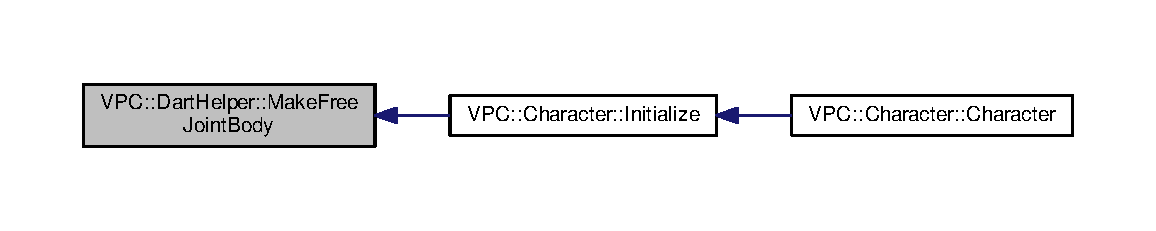
\includegraphics[width=350pt]{namespace_v_p_c_1_1_dart_helper_a69fa7c63ad96f84bb86411e438a73d48_icgraph}
\end{center}
\end{figure}


\index{V\+P\+C\+::\+Dart\+Helper@{V\+P\+C\+::\+Dart\+Helper}!Make\+Prismatic\+Joint\+Body@{Make\+Prismatic\+Joint\+Body}}
\index{Make\+Prismatic\+Joint\+Body@{Make\+Prismatic\+Joint\+Body}!V\+P\+C\+::\+Dart\+Helper@{V\+P\+C\+::\+Dart\+Helper}}
\subsubsection[{\texorpdfstring{Make\+Prismatic\+Joint\+Body(const std\+::string \&name, const dart\+::dynamics\+::\+Skeleton\+Ptr \&skel, dart\+::dynamics\+::\+Body\+Node $\ast$const parent, const Eigen\+::\+Vector3d \&size, const Eigen\+::\+Vector3d \&joint\+\_\+pos, const Eigen\+::\+Vector3d \&body\+\_\+pos, double mass)}{MakePrismaticJointBody(const std::string &name, const dart::dynamics::SkeletonPtr &skel, dart::dynamics::BodyNode *const parent, const Eigen::Vector3d &size, const Eigen::Vector3d &joint_pos, const Eigen::Vector3d &body_pos, double mass)}}]{\setlength{\rightskip}{0pt plus 5cm}dart\+::dynamics\+::\+Body\+Node $\ast$ V\+P\+C\+::\+Dart\+Helper\+::\+Make\+Prismatic\+Joint\+Body (
\begin{DoxyParamCaption}
\item[{const std\+::string \&}]{name, }
\item[{const dart\+::dynamics\+::\+Skeleton\+Ptr \&}]{skel, }
\item[{dart\+::dynamics\+::\+Body\+Node $\ast$const}]{parent, }
\item[{const Eigen\+::\+Vector3d \&}]{size, }
\item[{const Eigen\+::\+Vector3d \&}]{joint\+\_\+pos, }
\item[{const Eigen\+::\+Vector3d \&}]{body\+\_\+pos, }
\item[{double}]{mass}
\end{DoxyParamCaption}
)}\hypertarget{namespace_v_p_c_1_1_dart_helper_aca1fb6a9cadd2f260f0e20813d2c6c57}{}\label{namespace_v_p_c_1_1_dart_helper_aca1fb6a9cadd2f260f0e20813d2c6c57}


Definēts līnijā 70 failā Dart\+Helper.\+cpp.


\begin{DoxyCode}
78 \{
79     ShapePtr shape = std::shared\_ptr<BoxShape>(\textcolor{keyword}{new} BoxShape(size)); 
80 
81     dart::dynamics::Inertia inertia;
82     inertia.setMass(mass);
83     inertia.setMoment(shape->computeInertia(mass));
84 
85     BodyNode* bn;
86     PrismaticJoint::Properties props;
87     props.mName = name + \textcolor{stringliteral}{"\_joint"};
88     props.mAxis = Eigen::Vector3d::UnitX();
89 
90     \textcolor{keywordflow}{if}(parent!=\textcolor{keyword}{nullptr})
91     \{
92         \textcolor{keyword}{const} \textcolor{keyword}{auto} sn = parent->getShapeNodesWith<DynamicsAspect>();
93         \textcolor{keyword}{const} \textcolor{keyword}{auto} box = std::dynamic\_pointer\_cast<\textcolor{keyword}{const} BoxShape>(sn[0]->getShape());
94     \}   
95 
96     props.mT\_ParentBodyToJoint.setIdentity();
97     props.mT\_ParentBodyToJoint.translation() = body\_pos;
98 
99     bn = skel->createJointAndBodyNodePair<PrismaticJoint>(
100         parent,props,BodyNode::AspectProperties(name)).second;
101     bn->createShapeNodeWith<VisualAspect,CollisionAspect, DynamicsAspect>(shape);
102     
103     bn->setInertia(inertia);
104 
105     \textcolor{keywordflow}{return} bn;
106 \}
\end{DoxyCode}
\index{V\+P\+C\+::\+Dart\+Helper@{V\+P\+C\+::\+Dart\+Helper}!Make\+Revolute\+Joint\+Body@{Make\+Revolute\+Joint\+Body}}
\index{Make\+Revolute\+Joint\+Body@{Make\+Revolute\+Joint\+Body}!V\+P\+C\+::\+Dart\+Helper@{V\+P\+C\+::\+Dart\+Helper}}
\subsubsection[{\texorpdfstring{Make\+Revolute\+Joint\+Body(const std\+::string \&name, const dart\+::dynamics\+::\+Skeleton\+Ptr \&skel, dart\+::dynamics\+::\+Body\+Node $\ast$const parent, const Eigen\+::\+Vector3d \&size, const Eigen\+::\+Vector3d \&joint\+\_\+pos, const Eigen\+::\+Vector3d \&body\+\_\+pos, double mass)}{MakeRevoluteJointBody(const std::string &name, const dart::dynamics::SkeletonPtr &skel, dart::dynamics::BodyNode *const parent, const Eigen::Vector3d &size, const Eigen::Vector3d &joint_pos, const Eigen::Vector3d &body_pos, double mass)}}]{\setlength{\rightskip}{0pt plus 5cm}dart\+::dynamics\+::\+Body\+Node $\ast$ V\+P\+C\+::\+Dart\+Helper\+::\+Make\+Revolute\+Joint\+Body (
\begin{DoxyParamCaption}
\item[{const std\+::string \&}]{name, }
\item[{const dart\+::dynamics\+::\+Skeleton\+Ptr \&}]{skel, }
\item[{dart\+::dynamics\+::\+Body\+Node $\ast$const}]{parent, }
\item[{const Eigen\+::\+Vector3d \&}]{size, }
\item[{const Eigen\+::\+Vector3d \&}]{joint\+\_\+pos, }
\item[{const Eigen\+::\+Vector3d \&}]{body\+\_\+pos, }
\item[{double}]{mass}
\end{DoxyParamCaption}
)}\hypertarget{namespace_v_p_c_1_1_dart_helper_a4cf2225ca4d44189f0f0f390cf7aff99}{}\label{namespace_v_p_c_1_1_dart_helper_a4cf2225ca4d44189f0f0f390cf7aff99}


Definēts līnijā 107 failā Dart\+Helper.\+cpp.


\begin{DoxyCode}
115 \{
116     ShapePtr shape = std::shared\_ptr<BoxShape>(\textcolor{keyword}{new} BoxShape(size));
117 
118     dart::dynamics::Inertia inertia;
119     inertia.setMass(mass);
120     inertia.setMoment(shape->computeInertia(mass));
121 
122     BodyNode* bn;
123     RevoluteJoint::Properties props;
124     props.mName = name + \textcolor{stringliteral}{"\_joint"};
125     \textcolor{keywordflow}{if}(parent!=\textcolor{keyword}{nullptr})
126     \{
127         props.mT\_ParentBodyToJoint.setIdentity();
128         props.mT\_ParentBodyToJoint.translation() = joint\_pos-parent->getCOM();
129     \}
130 
131     props.mT\_ChildBodyToJoint.setIdentity();
132     props.mT\_ChildBodyToJoint.translation() = joint\_pos-body\_pos;
133     props.mAxis = Eigen::Vector3d::UnitZ();
134     bn = skel->createJointAndBodyNodePair<RevoluteJoint>(
135         parent,props,BodyNode::AspectProperties(name)).second;
136     bn->createShapeNodeWith<VisualAspect,CollisionAspect, DynamicsAspect>(shape);
137     
138     bn->setInertia(inertia);
139 
140     \textcolor{keywordflow}{return} bn;
141 \}
\end{DoxyCode}


Šeit ir šīs funkcijas izsaukuma grafs\+:
\nopagebreak
\begin{figure}[H]
\begin{center}
\leavevmode
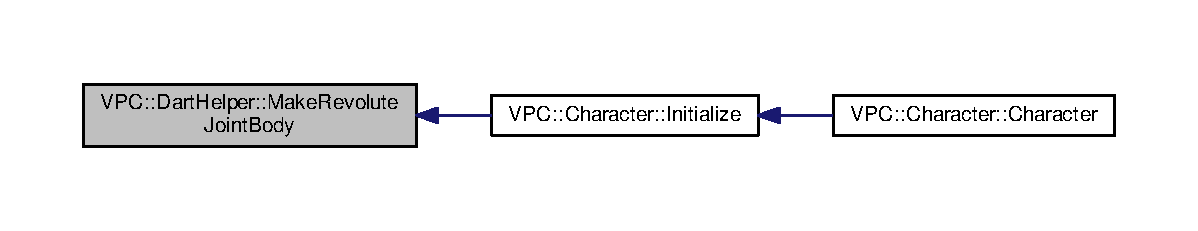
\includegraphics[width=350pt]{namespace_v_p_c_1_1_dart_helper_a4cf2225ca4d44189f0f0f390cf7aff99_icgraph}
\end{center}
\end{figure}


\index{V\+P\+C\+::\+Dart\+Helper@{V\+P\+C\+::\+Dart\+Helper}!Make\+Weld\+Joint\+Body@{Make\+Weld\+Joint\+Body}}
\index{Make\+Weld\+Joint\+Body@{Make\+Weld\+Joint\+Body}!V\+P\+C\+::\+Dart\+Helper@{V\+P\+C\+::\+Dart\+Helper}}
\subsubsection[{\texorpdfstring{Make\+Weld\+Joint\+Body(const std\+::string \&name, const dart\+::dynamics\+::\+Skeleton\+Ptr \&skel, dart\+::dynamics\+::\+Body\+Node $\ast$const parent, const Eigen\+::\+Vector3d \&size, const Eigen\+::\+Vector3d \&joint\+\_\+pos, const Eigen\+::\+Vector3d \&body\+\_\+pos, double mass)}{MakeWeldJointBody(const std::string &name, const dart::dynamics::SkeletonPtr &skel, dart::dynamics::BodyNode *const parent, const Eigen::Vector3d &size, const Eigen::Vector3d &joint_pos, const Eigen::Vector3d &body_pos, double mass)}}]{\setlength{\rightskip}{0pt plus 5cm}dart\+::dynamics\+::\+Body\+Node $\ast$ V\+P\+C\+::\+Dart\+Helper\+::\+Make\+Weld\+Joint\+Body (
\begin{DoxyParamCaption}
\item[{const std\+::string \&}]{name, }
\item[{const dart\+::dynamics\+::\+Skeleton\+Ptr \&}]{skel, }
\item[{dart\+::dynamics\+::\+Body\+Node $\ast$const}]{parent, }
\item[{const Eigen\+::\+Vector3d \&}]{size, }
\item[{const Eigen\+::\+Vector3d \&}]{joint\+\_\+pos, }
\item[{const Eigen\+::\+Vector3d \&}]{body\+\_\+pos, }
\item[{double}]{mass}
\end{DoxyParamCaption}
)}\hypertarget{namespace_v_p_c_1_1_dart_helper_a70dd049386ce8ba7d9fdb96407d8c3d3}{}\label{namespace_v_p_c_1_1_dart_helper_a70dd049386ce8ba7d9fdb96407d8c3d3}


Definēts līnijā 142 failā Dart\+Helper.\+cpp.


\begin{DoxyCode}
150 \{
151     ShapePtr shape = std::shared\_ptr<BoxShape>(\textcolor{keyword}{new} BoxShape(size));
152 
153     dart::dynamics::Inertia inertia;
154     inertia.setMass(mass);
155     inertia.setMoment(shape->computeInertia(mass));
156 
157     BodyNode* bn;
158     WeldJoint::Properties props;
159     props.mName = name + \textcolor{stringliteral}{"\_joint"};
160     \textcolor{keywordflow}{if}(parent!=\textcolor{keyword}{nullptr})
161     \{
162         props.mT\_ParentBodyToJoint.setIdentity();
163         props.mT\_ParentBodyToJoint.translation() = joint\_pos-parent->getCOM();
164     \}
165 
166     props.mT\_ChildBodyToJoint.setIdentity();
167     props.mT\_ChildBodyToJoint.translation() = joint\_pos-body\_pos;
168     bn = skel->createJointAndBodyNodePair<WeldJoint>(
169         parent,props,BodyNode::AspectProperties(name)).second;
170     bn->createShapeNodeWith<VisualAspect,CollisionAspect, DynamicsAspect>(shape);
171     
172     bn->setInertia(inertia);    
173 
174     \textcolor{keywordflow}{return} bn;
175 \}
\end{DoxyCode}


Šeit ir šīs funkcijas izsaukuma grafs\+:
\nopagebreak
\begin{figure}[H]
\begin{center}
\leavevmode
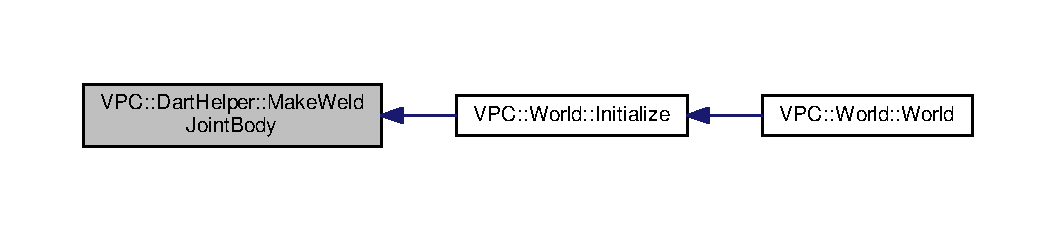
\includegraphics[width=350pt]{namespace_v_p_c_1_1_dart_helper_a70dd049386ce8ba7d9fdb96407d8c3d3_icgraph}
\end{center}
\end{figure}



\hypertarget{namespace_v_p_c_1_1_g_u_i}{}\section{V\+PC\+:\+:G\+UI nosaukumvietas apraksts}
\label{namespace_v_p_c_1_1_g_u_i}\index{V\+P\+C\+::\+G\+UI@{V\+P\+C\+::\+G\+UI}}
\subsection*{Nosaukumvietas}
\begin{DoxyCompactItemize}
\item 
 \hyperlink{namespace_v_p_c_1_1_g_u_i_1_1_dart_interface}{Dart\+Interface}
\end{DoxyCompactItemize}
\subsection*{Klases}
\begin{DoxyCompactItemize}
\item 
class \hyperlink{class_v_p_c_1_1_g_u_i_1_1_camera}{Camera}
\item 
class \hyperlink{class_v_p_c_1_1_g_u_i_1_1_g_l_u_t_window}{G\+L\+U\+T\+Window}
\item 
class \hyperlink{class_v_p_c_1_1_g_u_i_1_1_sim_window}{Sim\+Window}
\end{DoxyCompactItemize}
\subsection*{Funkcijas}
\begin{DoxyCompactItemize}
\item 
static void \hyperlink{namespace_v_p_c_1_1_g_u_i_a43f2493f014244094295c8840b9dc54f}{init\+Quad\+Obj} (void)
\item 
void \hyperlink{namespace_v_p_c_1_1_g_u_i_a7676fc36f15b67e72c9f1bd3a4836755}{Draw\+Point} (const Eigen\+::\+Vector3d \&p0, const Eigen\+::\+Vector4d \&color, double size)
\item 
void \hyperlink{namespace_v_p_c_1_1_g_u_i_a45de6c011f74c08734aa04ce57bb9fd7}{Draw\+Line} (const Eigen\+::\+Vector3d \&p0, const Eigen\+::\+Vector3d \&p1, const Eigen\+::\+Vector4d \&color, double width)
\item 
void \hyperlink{namespace_v_p_c_1_1_g_u_i_ae93b170c02a6812211061109cbb0c4a6}{Draw\+Sphere} (const Eigen\+::\+Vector3d \&p, double r, const Eigen\+::\+Vector4d \&color, int slices, int stacks)
\item 
void \hyperlink{namespace_v_p_c_1_1_g_u_i_a3ab06821c73e252bb864f2e9c9a6e916}{Draw\+Cube} (const Eigen\+::\+Isometry3d \&T, const Eigen\+::\+Vector3d \&\+\_\+size, const Eigen\+::\+Vector4d \&color)
\item 
void \hyperlink{namespace_v_p_c_1_1_g_u_i_a1021ea56c7215b6a592c0046a77677d2}{Draw\+Cylinder} (const Eigen\+::\+Isometry3d \&T, double \+\_\+radius, double \+\_\+height, const Eigen\+::\+Vector4d \&color, int slices, int stacks)
\item 
void \hyperlink{namespace_v_p_c_1_1_g_u_i_a727b1e8916ec599677fa11217d6ddf2b}{Draw\+Arrow3D} (const Eigen\+::\+Vector3d \&\+\_\+pt, const Eigen\+::\+Vector3d \&\+\_\+dir, const double \+\_\+length, const double \+\_\+thickness, const Eigen\+::\+Vector4d \&color, const double \+\_\+arrow\+Thickness)
\item 
void \hyperlink{namespace_v_p_c_1_1_g_u_i_a802b6ee2e4a882e55af30a5d12ff3965}{Draw\+Circle2D} (float \+\_\+x, float \+\_\+y, const std\+::string \&\+\_\+s, const Eigen\+::\+Vector4d \&color)
\item 
void \hyperlink{namespace_v_p_c_1_1_g_u_i_aba7cda15c9d9fa148f09e44915ec78f9}{Draw\+String\+On\+Screen} (float \+\_\+x, float \+\_\+y, const std\+::string \&\+\_\+s, bool \+\_\+big\+Font, const Eigen\+::\+Vector3d \&color)
\end{DoxyCompactItemize}
\subsection*{Mainīgie}
\begin{DoxyCompactItemize}
\item 
static G\+L\+Uquadric\+Obj $\ast$ \hyperlink{namespace_v_p_c_1_1_g_u_i_a0a2d963cfdc95564bad5be52225b4df8}{quad\+Obj}
\end{DoxyCompactItemize}


\subsection{Funkcijas dokumentācija}
\index{V\+P\+C\+::\+G\+UI@{V\+P\+C\+::\+G\+UI}!Draw\+Arrow3D@{Draw\+Arrow3D}}
\index{Draw\+Arrow3D@{Draw\+Arrow3D}!V\+P\+C\+::\+G\+UI@{V\+P\+C\+::\+G\+UI}}
\subsubsection[{\texorpdfstring{Draw\+Arrow3\+D(const Eigen\+::\+Vector3d \&\+\_\+pt, const Eigen\+::\+Vector3d \&\+\_\+dir, const double \+\_\+length, const double \+\_\+thickness, const Eigen\+::\+Vector4d \&color, const double \+\_\+arrow\+Thickness)}{DrawArrow3D(const Eigen::Vector3d &_pt, const Eigen::Vector3d &_dir, const double _length, const double _thickness, const Eigen::Vector4d &color, const double _arrowThickness)}}]{\setlength{\rightskip}{0pt plus 5cm}void V\+P\+C\+::\+G\+U\+I\+::\+Draw\+Arrow3D (
\begin{DoxyParamCaption}
\item[{const Eigen\+::\+Vector3d \&}]{\+\_\+pt, }
\item[{const Eigen\+::\+Vector3d \&}]{\+\_\+dir, }
\item[{const double}]{\+\_\+length, }
\item[{const double}]{\+\_\+thickness, }
\item[{const Eigen\+::\+Vector4d \&}]{color, }
\item[{const double}]{\+\_\+arrow\+Thickness}
\end{DoxyParamCaption}
)}\hypertarget{namespace_v_p_c_1_1_g_u_i_a727b1e8916ec599677fa11217d6ddf2b}{}\label{namespace_v_p_c_1_1_g_u_i_a727b1e8916ec599677fa11217d6ddf2b}


Definēts līnijā 122 failā G\+Lfunctions.\+cpp.


\begin{DoxyCode}
125 \{
126     glColor4d(color[0],color[1],color[2],color[3]);
127     Eigen::Vector3d normDir = \_dir;
128     normDir.normalize();
129 
130     \textcolor{keywordtype}{double} arrowLength;
131     \textcolor{keywordflow}{if} (\_arrowThickness == -1)
132     arrowLength = 4*\_thickness;
133     \textcolor{keywordflow}{else}
134     arrowLength = 2*\_arrowThickness;
135 
136     \textcolor{comment}{// draw the arrow body as a cylinder}
137     GLUquadricObj *c;
138     c = gluNewQuadric();
139     gluQuadricDrawStyle(c, GLU\_FILL);
140     gluQuadricNormals(c, GLU\_SMOOTH);
141 
142     glPushMatrix();
143     glTranslatef(\_pt[0], \_pt[1], \_pt[2]);
144     glRotated(acos(normDir[2])*180/M\_PI, -normDir[1], normDir[0], 0);
145     gluCylinder(c, \_thickness, \_thickness, \_length-arrowLength, 16, 16);
146 
147     glPopMatrix();
148 
149     gluDeleteQuadric(c);
150 \}
\end{DoxyCode}
\index{V\+P\+C\+::\+G\+UI@{V\+P\+C\+::\+G\+UI}!Draw\+Circle2D@{Draw\+Circle2D}}
\index{Draw\+Circle2D@{Draw\+Circle2D}!V\+P\+C\+::\+G\+UI@{V\+P\+C\+::\+G\+UI}}
\subsubsection[{\texorpdfstring{Draw\+Circle2\+D(float \+\_\+x, float \+\_\+y, const std\+::string \&\+\_\+s, const Eigen\+::\+Vector4d \&color)}{DrawCircle2D(float _x, float _y, const std::string &_s, const Eigen::Vector4d &color)}}]{\setlength{\rightskip}{0pt plus 5cm}void V\+P\+C\+::\+G\+U\+I\+::\+Draw\+Circle2D (
\begin{DoxyParamCaption}
\item[{float}]{\+\_\+x, }
\item[{float}]{\+\_\+y, }
\item[{const std\+::string \&}]{\+\_\+s, }
\item[{const Eigen\+::\+Vector4d \&}]{color}
\end{DoxyParamCaption}
)}\hypertarget{namespace_v_p_c_1_1_g_u_i_a802b6ee2e4a882e55af30a5d12ff3965}{}\label{namespace_v_p_c_1_1_g_u_i_a802b6ee2e4a882e55af30a5d12ff3965}


Definēts līnijā 153 failā G\+Lfunctions.\+cpp.


\begin{DoxyCode}
154 \{
155     
156     \textcolor{comment}{// draws text on the screen}
157     GLint oldMode;
158     glGetIntegerv(GL\_MATRIX\_MODE, &oldMode);
159     glMatrixMode(GL\_PROJECTION);
160 
161     glPushMatrix();
162     glLoadIdentity();
163     gluOrtho2D(0.0, 1.0, 0.0, 1.0);
164 
165     glMatrixMode(GL\_MODELVIEW);
166     glPushMatrix();
167     glLoadIdentity();
168     glColor4f(0,0,0,1.0);
169 
170     glRasterPos2f(\_x-0.005*\_s.length(), \_y-0.005);
171     
172     \textcolor{keywordtype}{unsigned} \textcolor{keywordtype}{int} length = \_s.length();
173     \textcolor{keywordflow}{for} (\textcolor{keywordtype}{unsigned} \textcolor{keywordtype}{int} c = 0; c < length; c++) \{
174       glutBitmapCharacter(GLUT\_BITMAP\_HELVETICA\_18, \_s.at(c) );
175     \}  
176     glPushMatrix();
177     glColor4d(color[0],color[1],color[2],0.4);
178 
179     glTranslatef(\_x,\_y,0);
180     glutSolidSphere(0.025,40,40);
181     glPopMatrix();
182     glPopMatrix();
183 
184     glMatrixMode(GL\_PROJECTION);
185     glPopMatrix();
186     glMatrixMode(oldMode);
187 \}
\end{DoxyCode}
\index{V\+P\+C\+::\+G\+UI@{V\+P\+C\+::\+G\+UI}!Draw\+Cube@{Draw\+Cube}}
\index{Draw\+Cube@{Draw\+Cube}!V\+P\+C\+::\+G\+UI@{V\+P\+C\+::\+G\+UI}}
\subsubsection[{\texorpdfstring{Draw\+Cube(const Eigen\+::\+Isometry3d \&\+T, const Eigen\+::\+Vector3d \&\+\_\+size, const Eigen\+::\+Vector4d \&color)}{DrawCube(const Eigen::Isometry3d &T, const Eigen::Vector3d &_size, const Eigen::Vector4d &color)}}]{\setlength{\rightskip}{0pt plus 5cm}void V\+P\+C\+::\+G\+U\+I\+::\+Draw\+Cube (
\begin{DoxyParamCaption}
\item[{const Eigen\+::\+Isometry3d \&}]{T, }
\item[{const Eigen\+::\+Vector3d \&}]{\+\_\+size, }
\item[{const Eigen\+::\+Vector4d \&}]{color}
\end{DoxyParamCaption}
)}\hypertarget{namespace_v_p_c_1_1_g_u_i_a3ab06821c73e252bb864f2e9c9a6e916}{}\label{namespace_v_p_c_1_1_g_u_i_a3ab06821c73e252bb864f2e9c9a6e916}


Definēts līnijā 50 failā G\+Lfunctions.\+cpp.


\begin{DoxyCode}
51 \{
52     glColor4d(color[0],color[1],color[2],color[3]);
53     glPushMatrix();
54     glMultMatrixd(T.data());
55     glScaled(\_size(0), \_size(1), \_size(2));
56 
57     
58 
59     \textcolor{comment}{// Code taken from glut/lib/glut\_shapes.c}
60     \textcolor{keyword}{static} GLfloat n[6][3] =
61     \{
62         \{-1.0, 0.0, 0.0\},
63         \{0.0, 1.0, 0.0\},
64         \{1.0, 0.0, 0.0\},
65         \{0.0, -1.0, 0.0\},
66         \{0.0, 0.0, 1.0\},
67         \{0.0, 0.0, -1.0\}
68     \};
69     \textcolor{keyword}{static} GLint faces[6][4] =
70     \{
71         \{0, 1, 2, 3\},
72         \{3, 2, 6, 7\},
73         \{7, 6, 5, 4\},
74         \{4, 5, 1, 0\},
75         \{5, 6, 2, 1\},
76         \{7, 4, 0, 3\}
77     \};
78     GLfloat v[8][3];
79     GLint i;
80     GLfloat size = 1;
81 
82     v[0][0] = v[1][0] = v[2][0] = v[3][0] = -size / 2;
83     v[4][0] = v[5][0] = v[6][0] = v[7][0] = size / 2;
84     v[0][1] = v[1][1] = v[4][1] = v[5][1] = -size / 2;
85     v[2][1] = v[3][1] = v[6][1] = v[7][1] = size / 2;
86     v[0][2] = v[3][2] = v[4][2] = v[7][2] = -size / 2;
87     v[1][2] = v[2][2] = v[5][2] = v[6][2] = size / 2;
88 
89     \textcolor{keywordflow}{for} (i = 5; i >= 0; i--) \{
90         glBegin(GL\_QUADS);
91         glNormal3fv(&n[i][0]);
92         glVertex3fv(&v[faces[i][0]][0]);
93         glVertex3fv(&v[faces[i][1]][0]);
94         glVertex3fv(&v[faces[i][2]][0]);
95         glVertex3fv(&v[faces[i][3]][0]);
96         glEnd();
97     \}
98     glPopMatrix();
99 \}
\end{DoxyCode}


Šeit ir šīs funkcijas izsaukuma grafs\+:
\nopagebreak
\begin{figure}[H]
\begin{center}
\leavevmode
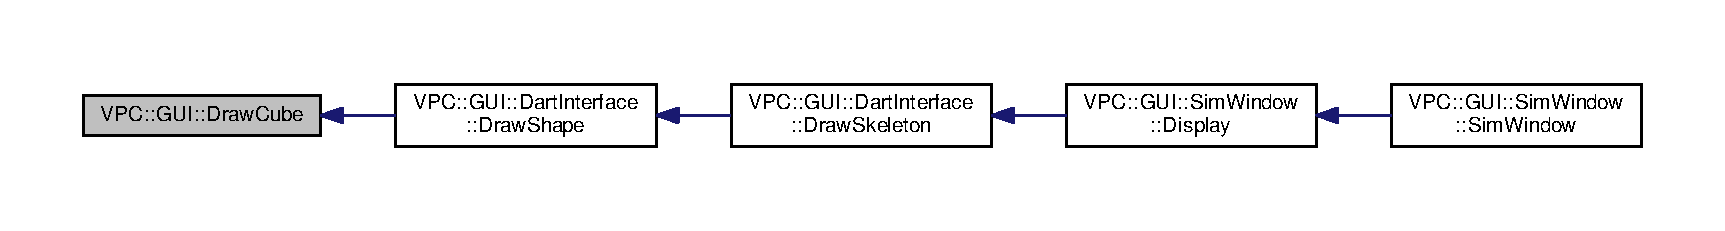
\includegraphics[width=350pt]{namespace_v_p_c_1_1_g_u_i_a3ab06821c73e252bb864f2e9c9a6e916_icgraph}
\end{center}
\end{figure}


\index{V\+P\+C\+::\+G\+UI@{V\+P\+C\+::\+G\+UI}!Draw\+Cylinder@{Draw\+Cylinder}}
\index{Draw\+Cylinder@{Draw\+Cylinder}!V\+P\+C\+::\+G\+UI@{V\+P\+C\+::\+G\+UI}}
\subsubsection[{\texorpdfstring{Draw\+Cylinder(const Eigen\+::\+Isometry3d \&\+T, double \+\_\+radius, double \+\_\+height, const Eigen\+::\+Vector4d \&color, int slices, int stacks)}{DrawCylinder(const Eigen::Isometry3d &T, double _radius, double _height, const Eigen::Vector4d &color, int slices, int stacks)}}]{\setlength{\rightskip}{0pt plus 5cm}void V\+P\+C\+::\+G\+U\+I\+::\+Draw\+Cylinder (
\begin{DoxyParamCaption}
\item[{const Eigen\+::\+Isometry3d \&}]{T, }
\item[{double}]{\+\_\+radius, }
\item[{double}]{\+\_\+height, }
\item[{const Eigen\+::\+Vector4d \&}]{color, }
\item[{int}]{slices, }
\item[{int}]{stacks}
\end{DoxyParamCaption}
)}\hypertarget{namespace_v_p_c_1_1_g_u_i_a1021ea56c7215b6a592c0046a77677d2}{}\label{namespace_v_p_c_1_1_g_u_i_a1021ea56c7215b6a592c0046a77677d2}


Definēts līnijā 105 failā G\+Lfunctions.\+cpp.


\begin{DoxyCode}
106 \{
107     glColor4d(color[0],color[1],color[2],color[3]);
108     glPushMatrix();
109     glMultMatrixd(T.data());
110     glTranslated(0.0, 0.0, -0.5*\_height);
111 
112     \hyperlink{_g_lfunctions_8cpp_ac0622674f5e3b0eb0bb851ca8d546b34}{QUAD\_OBJ\_INIT};
113     gluQuadricDrawStyle(\hyperlink{namespace_v_p_c_1_1_g_u_i_a0a2d963cfdc95564bad5be52225b4df8}{quadObj}, GLU\_FILL);
114     gluQuadricNormals(\hyperlink{namespace_v_p_c_1_1_g_u_i_a0a2d963cfdc95564bad5be52225b4df8}{quadObj}, GLU\_SMOOTH);
115 
116     gluCylinder(\hyperlink{namespace_v_p_c_1_1_g_u_i_a0a2d963cfdc95564bad5be52225b4df8}{quadObj}, \_radius, \_radius, \_height, slices, stacks);
117     glPopMatrix();
118 \}
\end{DoxyCode}
\index{V\+P\+C\+::\+G\+UI@{V\+P\+C\+::\+G\+UI}!Draw\+Line@{Draw\+Line}}
\index{Draw\+Line@{Draw\+Line}!V\+P\+C\+::\+G\+UI@{V\+P\+C\+::\+G\+UI}}
\subsubsection[{\texorpdfstring{Draw\+Line(const Eigen\+::\+Vector3d \&p0, const Eigen\+::\+Vector3d \&p1, const Eigen\+::\+Vector4d \&color, double width)}{DrawLine(const Eigen::Vector3d &p0, const Eigen::Vector3d &p1, const Eigen::Vector4d &color, double width)}}]{\setlength{\rightskip}{0pt plus 5cm}void V\+P\+C\+::\+G\+U\+I\+::\+Draw\+Line (
\begin{DoxyParamCaption}
\item[{const Eigen\+::\+Vector3d \&}]{p0, }
\item[{const Eigen\+::\+Vector3d \&}]{p1, }
\item[{const Eigen\+::\+Vector4d \&}]{color, }
\item[{double}]{width}
\end{DoxyParamCaption}
)}\hypertarget{namespace_v_p_c_1_1_g_u_i_a45de6c011f74c08734aa04ce57bb9fd7}{}\label{namespace_v_p_c_1_1_g_u_i_a45de6c011f74c08734aa04ce57bb9fd7}


Definēts līnijā 27 failā G\+Lfunctions.\+cpp.


\begin{DoxyCode}
28 \{
29     glColor4d(color[0],color[1],color[2],color[3]);
30     glLineWidth(width);
31     glBegin(GL\_LINES);
32     glVertex3d(p0[0],p0[1],p0[2]);
33     glVertex3d(p1[0],p1[1],p1[2]);
34     glEnd();
35 \}
\end{DoxyCode}


Šeit ir šīs funkcijas izsaukuma grafs\+:
\nopagebreak
\begin{figure}[H]
\begin{center}
\leavevmode
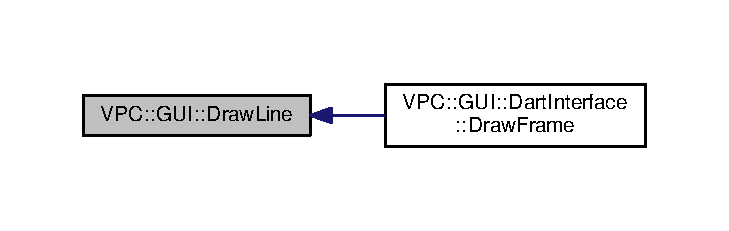
\includegraphics[width=350pt]{namespace_v_p_c_1_1_g_u_i_a45de6c011f74c08734aa04ce57bb9fd7_icgraph}
\end{center}
\end{figure}


\index{V\+P\+C\+::\+G\+UI@{V\+P\+C\+::\+G\+UI}!Draw\+Point@{Draw\+Point}}
\index{Draw\+Point@{Draw\+Point}!V\+P\+C\+::\+G\+UI@{V\+P\+C\+::\+G\+UI}}
\subsubsection[{\texorpdfstring{Draw\+Point(const Eigen\+::\+Vector3d \&p0, const Eigen\+::\+Vector4d \&color, double size)}{DrawPoint(const Eigen::Vector3d &p0, const Eigen::Vector4d &color, double size)}}]{\setlength{\rightskip}{0pt plus 5cm}void V\+P\+C\+::\+G\+U\+I\+::\+Draw\+Point (
\begin{DoxyParamCaption}
\item[{const Eigen\+::\+Vector3d \&}]{p0, }
\item[{const Eigen\+::\+Vector4d \&}]{color, }
\item[{double}]{size}
\end{DoxyParamCaption}
)}\hypertarget{namespace_v_p_c_1_1_g_u_i_a7676fc36f15b67e72c9f1bd3a4836755}{}\label{namespace_v_p_c_1_1_g_u_i_a7676fc36f15b67e72c9f1bd3a4836755}


Definēts līnijā 18 failā G\+Lfunctions.\+cpp.


\begin{DoxyCode}
19 \{
20     glColor4d(color[0],color[1],color[2],color[3]);
21     glPointSize(size);
22     glBegin(GL\_POINTS);
23     glVertex3d(p0[0],p0[1],p0[2]);
24     glEnd();
25 \}
\end{DoxyCode}
\index{V\+P\+C\+::\+G\+UI@{V\+P\+C\+::\+G\+UI}!Draw\+Sphere@{Draw\+Sphere}}
\index{Draw\+Sphere@{Draw\+Sphere}!V\+P\+C\+::\+G\+UI@{V\+P\+C\+::\+G\+UI}}
\subsubsection[{\texorpdfstring{Draw\+Sphere(const Eigen\+::\+Vector3d \&p, double r, const Eigen\+::\+Vector4d \&color, int slices, int stacks)}{DrawSphere(const Eigen::Vector3d &p, double r, const Eigen::Vector4d &color, int slices, int stacks)}}]{\setlength{\rightskip}{0pt plus 5cm}void V\+P\+C\+::\+G\+U\+I\+::\+Draw\+Sphere (
\begin{DoxyParamCaption}
\item[{const Eigen\+::\+Vector3d \&}]{p, }
\item[{double}]{r, }
\item[{const Eigen\+::\+Vector4d \&}]{color, }
\item[{int}]{slices, }
\item[{int}]{stacks}
\end{DoxyParamCaption}
)}\hypertarget{namespace_v_p_c_1_1_g_u_i_ae93b170c02a6812211061109cbb0c4a6}{}\label{namespace_v_p_c_1_1_g_u_i_ae93b170c02a6812211061109cbb0c4a6}


Definēts līnijā 37 failā G\+Lfunctions.\+cpp.


\begin{DoxyCode}
38 \{
39     \hyperlink{_g_lfunctions_8cpp_ac0622674f5e3b0eb0bb851ca8d546b34}{QUAD\_OBJ\_INIT};
40     gluQuadricDrawStyle(\hyperlink{namespace_v_p_c_1_1_g_u_i_a0a2d963cfdc95564bad5be52225b4df8}{quadObj}, GLU\_FILL);
41     gluQuadricNormals(\hyperlink{namespace_v_p_c_1_1_g_u_i_a0a2d963cfdc95564bad5be52225b4df8}{quadObj}, GLU\_SMOOTH);
42     glColor4d(color[0],color[1],color[2],color[3]);
43     glPushMatrix();
44     glTranslated(p[0],p[1],p[2]);
45     gluSphere(\hyperlink{namespace_v_p_c_1_1_g_u_i_a0a2d963cfdc95564bad5be52225b4df8}{quadObj}, \hyperlink{namespaceddpg__others_a05079a0e5b9b284648a5e279d844fc34}{r}, 16, 16);
46     glPopMatrix();
47 \}
\end{DoxyCode}


Šeit ir šīs funkcijas izsaukuma grafs\+:
\nopagebreak
\begin{figure}[H]
\begin{center}
\leavevmode
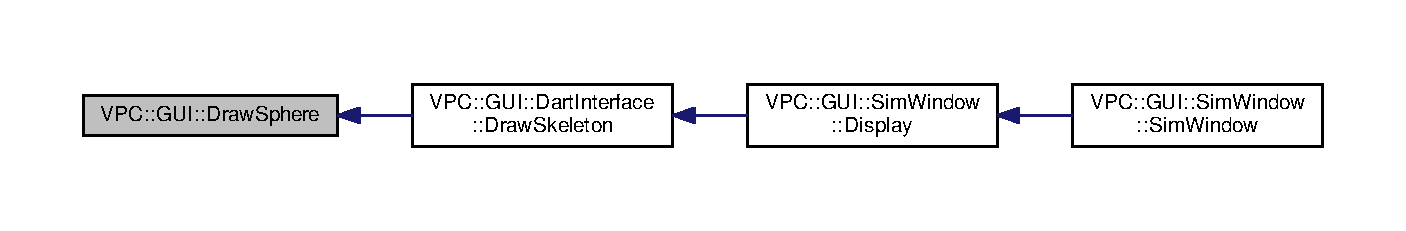
\includegraphics[width=350pt]{namespace_v_p_c_1_1_g_u_i_ae93b170c02a6812211061109cbb0c4a6_icgraph}
\end{center}
\end{figure}


\index{V\+P\+C\+::\+G\+UI@{V\+P\+C\+::\+G\+UI}!Draw\+String\+On\+Screen@{Draw\+String\+On\+Screen}}
\index{Draw\+String\+On\+Screen@{Draw\+String\+On\+Screen}!V\+P\+C\+::\+G\+UI@{V\+P\+C\+::\+G\+UI}}
\subsubsection[{\texorpdfstring{Draw\+String\+On\+Screen(float \+\_\+x, float \+\_\+y, const std\+::string \&\+\_\+s, bool \+\_\+big\+Font, const Eigen\+::\+Vector3d \&color)}{DrawStringOnScreen(float _x, float _y, const std::string &_s, bool _bigFont, const Eigen::Vector3d &color)}}]{\setlength{\rightskip}{0pt plus 5cm}void V\+P\+C\+::\+G\+U\+I\+::\+Draw\+String\+On\+Screen (
\begin{DoxyParamCaption}
\item[{float}]{\+\_\+x, }
\item[{float}]{\+\_\+y, }
\item[{const std\+::string \&}]{\+\_\+s, }
\item[{bool}]{\+\_\+big\+Font, }
\item[{const Eigen\+::\+Vector3d \&}]{color}
\end{DoxyParamCaption}
)}\hypertarget{namespace_v_p_c_1_1_g_u_i_aba7cda15c9d9fa148f09e44915ec78f9}{}\label{namespace_v_p_c_1_1_g_u_i_aba7cda15c9d9fa148f09e44915ec78f9}


Definēts līnijā 189 failā G\+Lfunctions.\+cpp.


\begin{DoxyCode}
190 \{
191     glColor3f(color[0],color[1],color[2]);
192     
193     \textcolor{comment}{// draws text on the screen}
194     GLint oldMode;
195     glGetIntegerv(GL\_MATRIX\_MODE, &oldMode);
196     glMatrixMode(GL\_PROJECTION);
197 
198     glPushMatrix();
199     glLoadIdentity();
200     gluOrtho2D(0.0, 1.0, 0.0, 1.0);
201 
202     glMatrixMode(GL\_MODELVIEW);
203     glPushMatrix();
204     glLoadIdentity();
205     glRasterPos2f(\_x, \_y);
206     \textcolor{keywordtype}{unsigned} \textcolor{keywordtype}{int} length = \_s.length();
207     \textcolor{keywordflow}{for} (\textcolor{keywordtype}{unsigned} \textcolor{keywordtype}{int} c = 0; c < length; c++) \{
208     \textcolor{keywordflow}{if} (\_bigFont)
209       glutBitmapCharacter(GLUT\_BITMAP\_HELVETICA\_18, \_s.at(c) );
210     \textcolor{keywordflow}{else}
211       glutBitmapCharacter(GLUT\_BITMAP\_HELVETICA\_10, \_s.at(c) );
212     \}  
213     glPopMatrix();
214 
215     glMatrixMode(GL\_PROJECTION);
216     glPopMatrix();
217     glMatrixMode(oldMode);
218 \}
\end{DoxyCode}


Šeit ir šīs funkcijas izsaukuma grafs\+:
\nopagebreak
\begin{figure}[H]
\begin{center}
\leavevmode
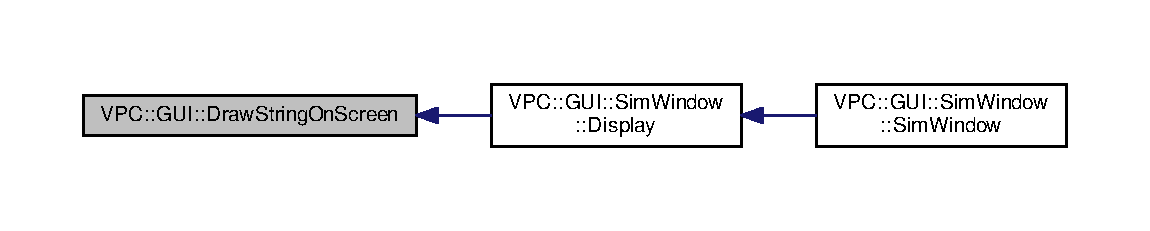
\includegraphics[width=350pt]{namespace_v_p_c_1_1_g_u_i_aba7cda15c9d9fa148f09e44915ec78f9_icgraph}
\end{center}
\end{figure}


\index{V\+P\+C\+::\+G\+UI@{V\+P\+C\+::\+G\+UI}!init\+Quad\+Obj@{init\+Quad\+Obj}}
\index{init\+Quad\+Obj@{init\+Quad\+Obj}!V\+P\+C\+::\+G\+UI@{V\+P\+C\+::\+G\+UI}}
\subsubsection[{\texorpdfstring{init\+Quad\+Obj(void)}{initQuadObj(void)}}]{\setlength{\rightskip}{0pt plus 5cm}static void V\+P\+C\+::\+G\+U\+I\+::init\+Quad\+Obj (
\begin{DoxyParamCaption}
\item[{void}]{}
\end{DoxyParamCaption}
)\hspace{0.3cm}{\ttfamily [static]}}\hypertarget{namespace_v_p_c_1_1_g_u_i_a43f2493f014244094295c8840b9dc54f}{}\label{namespace_v_p_c_1_1_g_u_i_a43f2493f014244094295c8840b9dc54f}


Definēts līnijā 8 failā G\+Lfunctions.\+cpp.


\begin{DoxyCode}
9 \{
10     \hyperlink{namespace_v_p_c_1_1_g_u_i_a0a2d963cfdc95564bad5be52225b4df8}{quadObj} = gluNewQuadric();
11     \textcolor{keywordflow}{if}(!\hyperlink{namespace_v_p_c_1_1_g_u_i_a0a2d963cfdc95564bad5be52225b4df8}{quadObj})
12         \textcolor{comment}{// DART modified error output}
13         std::cerr << \textcolor{stringliteral}{"OpenGL: Fatal Error in DART: out of memory."} << std::endl;
14 \}
\end{DoxyCode}


\subsection{Mainīgo dokumentācija}
\index{V\+P\+C\+::\+G\+UI@{V\+P\+C\+::\+G\+UI}!quad\+Obj@{quad\+Obj}}
\index{quad\+Obj@{quad\+Obj}!V\+P\+C\+::\+G\+UI@{V\+P\+C\+::\+G\+UI}}
\subsubsection[{\texorpdfstring{quad\+Obj}{quadObj}}]{\setlength{\rightskip}{0pt plus 5cm}G\+L\+Uquadric\+Obj$\ast$ V\+P\+C\+::\+G\+U\+I\+::quad\+Obj\hspace{0.3cm}{\ttfamily [static]}}\hypertarget{namespace_v_p_c_1_1_g_u_i_a0a2d963cfdc95564bad5be52225b4df8}{}\label{namespace_v_p_c_1_1_g_u_i_a0a2d963cfdc95564bad5be52225b4df8}


Definēts līnijā 7 failā G\+Lfunctions.\+cpp.


\hypertarget{namespace_v_p_c_1_1_g_u_i_1_1_dart_interface}{}\section{V\+PC\+:\+:G\+UI\+:\+:Dart\+Interface nosaukumvietas apraksts}
\label{namespace_v_p_c_1_1_g_u_i_1_1_dart_interface}\index{V\+P\+C\+::\+G\+U\+I\+::\+Dart\+Interface@{V\+P\+C\+::\+G\+U\+I\+::\+Dart\+Interface}}
\subsection*{Funkcijas}
\begin{DoxyCompactItemize}
\item 
void \hyperlink{namespace_v_p_c_1_1_g_u_i_1_1_dart_interface_a81b02a78bdeb3f5bdd750d8357f6f426}{Draw\+Shape} (const Eigen\+::\+Isometry3d \&T, const dart\+::dynamics\+::\+Shape $\ast$shape, const Eigen\+::\+Vector4d \&color)
\item 
void \hyperlink{namespace_v_p_c_1_1_g_u_i_1_1_dart_interface_a984d0004c2f1a3006835ec469c1318d3}{Draw\+Frame} (const Eigen\+::\+Isometry3d \&T)
\item 
void \hyperlink{namespace_v_p_c_1_1_g_u_i_1_1_dart_interface_a0f48bc6711d69c0979519f00998d1876}{Draw\+Skeleton} (const dart\+::dynamics\+::\+Skeleton\+Ptr \&skel, const Eigen\+::\+Vector4d \&color)
\end{DoxyCompactItemize}


\subsection{Funkcijas dokumentācija}
\index{V\+P\+C\+::\+G\+U\+I\+::\+Dart\+Interface@{V\+P\+C\+::\+G\+U\+I\+::\+Dart\+Interface}!Draw\+Frame@{Draw\+Frame}}
\index{Draw\+Frame@{Draw\+Frame}!V\+P\+C\+::\+G\+U\+I\+::\+Dart\+Interface@{V\+P\+C\+::\+G\+U\+I\+::\+Dart\+Interface}}
\subsubsection[{\texorpdfstring{Draw\+Frame(const Eigen\+::\+Isometry3d \&\+T)}{DrawFrame(const Eigen::Isometry3d &T)}}]{\setlength{\rightskip}{0pt plus 5cm}void V\+P\+C\+::\+G\+U\+I\+::\+Dart\+Interface\+::\+Draw\+Frame (
\begin{DoxyParamCaption}
\item[{const Eigen\+::\+Isometry3d \&}]{T}
\end{DoxyParamCaption}
)}\hypertarget{namespace_v_p_c_1_1_g_u_i_1_1_dart_interface_a984d0004c2f1a3006835ec469c1318d3}{}\label{namespace_v_p_c_1_1_g_u_i_1_1_dart_interface_a984d0004c2f1a3006835ec469c1318d3}


Definēts līnijā 63 failā Dart\+Interface.\+cpp.


\begin{DoxyCode}
64 \{
65     Eigen::Vector3d p0,p1;
66     glDisable(GL\_LIGHTING);
67     glPushMatrix();
68     glMultMatrixd(T.data());
69     p0 = Eigen::Vector3d::Zero();
70 
71     p1 = 0.1*Eigen::Vector3d::UnitX();
72     \hyperlink{namespace_v_p_c_1_1_g_u_i_a45de6c011f74c08734aa04ce57bb9fd7}{DrawLine}(p0,p1,Eigen::Vector4d(1,0,0,1),2.0);
73     p1 = 0.1*Eigen::Vector3d::UnitY();
74     \hyperlink{namespace_v_p_c_1_1_g_u_i_a45de6c011f74c08734aa04ce57bb9fd7}{DrawLine}(p0,p1,Eigen::Vector4d(0,1,0,1),2.0);
75     p1 = 0.1*Eigen::Vector3d::UnitZ();
76     \hyperlink{namespace_v_p_c_1_1_g_u_i_a45de6c011f74c08734aa04ce57bb9fd7}{DrawLine}(p0,p1,Eigen::Vector4d(0,0,1,1),2.0);
77     glPopMatrix();
78     glEnable(GL\_LIGHTING);
79 \}
\end{DoxyCode}


Šeit ir visu funkciju izsaugumu grafs\+:
\nopagebreak
\begin{figure}[H]
\begin{center}
\leavevmode
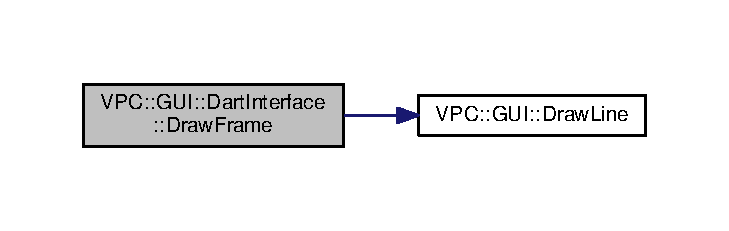
\includegraphics[width=350pt]{namespace_v_p_c_1_1_g_u_i_1_1_dart_interface_a984d0004c2f1a3006835ec469c1318d3_cgraph}
\end{center}
\end{figure}


\index{V\+P\+C\+::\+G\+U\+I\+::\+Dart\+Interface@{V\+P\+C\+::\+G\+U\+I\+::\+Dart\+Interface}!Draw\+Shape@{Draw\+Shape}}
\index{Draw\+Shape@{Draw\+Shape}!V\+P\+C\+::\+G\+U\+I\+::\+Dart\+Interface@{V\+P\+C\+::\+G\+U\+I\+::\+Dart\+Interface}}
\subsubsection[{\texorpdfstring{Draw\+Shape(const Eigen\+::\+Isometry3d \&\+T, const dart\+::dynamics\+::\+Shape $\ast$shape, const Eigen\+::\+Vector4d \&color)}{DrawShape(const Eigen::Isometry3d &T, const dart::dynamics::Shape *shape, const Eigen::Vector4d &color)}}]{\setlength{\rightskip}{0pt plus 5cm}void V\+P\+C\+::\+G\+U\+I\+::\+Dart\+Interface\+::\+Draw\+Shape (
\begin{DoxyParamCaption}
\item[{const Eigen\+::\+Isometry3d \&}]{T, }
\item[{const dart\+::dynamics\+::\+Shape $\ast$}]{shape, }
\item[{const Eigen\+::\+Vector4d \&}]{color}
\end{DoxyParamCaption}
)}\hypertarget{namespace_v_p_c_1_1_g_u_i_1_1_dart_interface_a81b02a78bdeb3f5bdd750d8357f6f426}{}\label{namespace_v_p_c_1_1_g_u_i_1_1_dart_interface_a81b02a78bdeb3f5bdd750d8357f6f426}


Definēts līnijā 47 failā Dart\+Interface.\+cpp.


\begin{DoxyCode}
50 \{
51 
52     glEnable(GL\_LIGHTING);
53     glColorMaterial(GL\_FRONT\_AND\_BACK, GL\_AMBIENT\_AND\_DIFFUSE);
54     glEnable(GL\_COLOR\_MATERIAL);
55     \textcolor{keywordflow}{if} (shape->is<BoxShape>())
56     \{
57         \textcolor{keyword}{const} \textcolor{keyword}{auto}* box = \textcolor{keyword}{dynamic\_cast<}\textcolor{keyword}{const }BoxShape*\textcolor{keyword}{>}(shape);
58         glPolygonMode(GL\_FRONT\_AND\_BACK,GL\_FILL);
59         \hyperlink{namespace_v_p_c_1_1_g_u_i_a3ab06821c73e252bb864f2e9c9a6e916}{DrawCube}(T,box->getSize(),color);
60     \}
61     glDisable(GL\_LIGHTING);
62 \}
\end{DoxyCode}


Šeit ir visu funkciju izsaugumu grafs\+:
\nopagebreak
\begin{figure}[H]
\begin{center}
\leavevmode
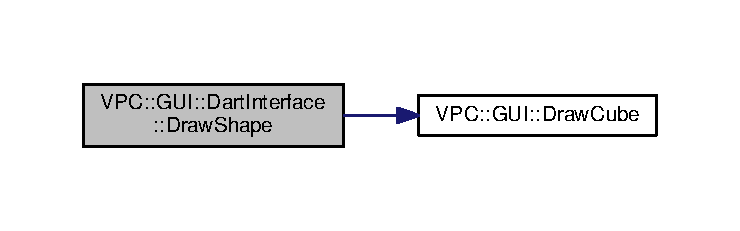
\includegraphics[width=350pt]{namespace_v_p_c_1_1_g_u_i_1_1_dart_interface_a81b02a78bdeb3f5bdd750d8357f6f426_cgraph}
\end{center}
\end{figure}




Šeit ir šīs funkcijas izsaukuma grafs\+:
\nopagebreak
\begin{figure}[H]
\begin{center}
\leavevmode
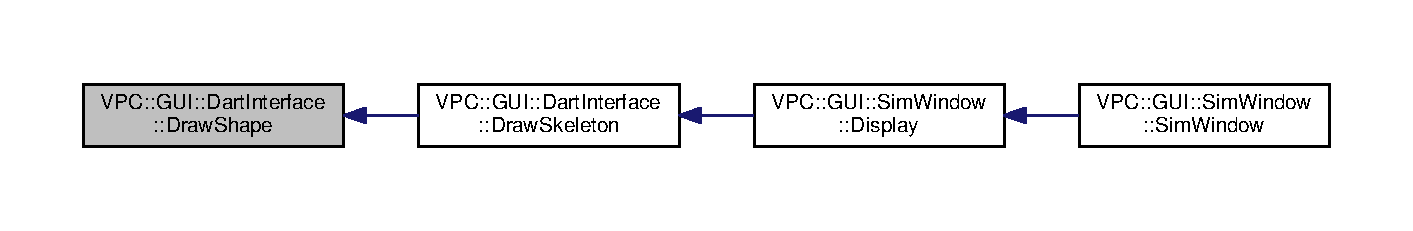
\includegraphics[width=350pt]{namespace_v_p_c_1_1_g_u_i_1_1_dart_interface_a81b02a78bdeb3f5bdd750d8357f6f426_icgraph}
\end{center}
\end{figure}


\index{V\+P\+C\+::\+G\+U\+I\+::\+Dart\+Interface@{V\+P\+C\+::\+G\+U\+I\+::\+Dart\+Interface}!Draw\+Skeleton@{Draw\+Skeleton}}
\index{Draw\+Skeleton@{Draw\+Skeleton}!V\+P\+C\+::\+G\+U\+I\+::\+Dart\+Interface@{V\+P\+C\+::\+G\+U\+I\+::\+Dart\+Interface}}
\subsubsection[{\texorpdfstring{Draw\+Skeleton(const dart\+::dynamics\+::\+Skeleton\+Ptr \&skel, const Eigen\+::\+Vector4d \&color)}{DrawSkeleton(const dart::dynamics::SkeletonPtr &skel, const Eigen::Vector4d &color)}}]{\setlength{\rightskip}{0pt plus 5cm}void V\+P\+C\+::\+G\+U\+I\+::\+Dart\+Interface\+::\+Draw\+Skeleton (
\begin{DoxyParamCaption}
\item[{const dart\+::dynamics\+::\+Skeleton\+Ptr \&}]{skel, }
\item[{const Eigen\+::\+Vector4d \&}]{color}
\end{DoxyParamCaption}
)}\hypertarget{namespace_v_p_c_1_1_g_u_i_1_1_dart_interface_a0f48bc6711d69c0979519f00998d1876}{}\label{namespace_v_p_c_1_1_g_u_i_1_1_dart_interface_a0f48bc6711d69c0979519f00998d1876}


Definēts līnijā 15 failā Dart\+Interface.\+cpp.


\begin{DoxyCode}
18 \{
19     \textcolor{keywordflow}{for}(\textcolor{keywordtype}{int} i=0;i<skel->getNumBodyNodes();i++)
20     \{
21         \textcolor{keyword}{auto} bn = skel->getBodyNode(i);
22         \textcolor{keyword}{auto} shapeNodes = bn->getShapeNodesWith<VisualAspect>();
23 
24         \textcolor{comment}{// const Eigen::Isometry3d& T = shapeNodes[0]->getTransform();}
25         \textcolor{keyword}{const} Eigen::Isometry3d& T = bn->getTransform();
26         
27         \hyperlink{namespace_v_p_c_1_1_g_u_i_1_1_dart_interface_a81b02a78bdeb3f5bdd750d8357f6f426}{DrawShape}(T,shapeNodes[0]->getShape().\textcolor{keyword}{get}(),color);
28         \textcolor{comment}{// glDisable(GL\_DEPTH\_TEST);}
29         \textcolor{comment}{// DrawFrame(T);}
30         \textcolor{comment}{// glEnable(GL\_DEPTH\_TEST);}
31     \}   
32     glDisable(GL\_DEPTH\_TEST);
33     \textcolor{keywordflow}{for}(\textcolor{keywordtype}{int} i = 1;i<skel->getNumJoints();i++)
34     \{
35         \textcolor{keyword}{auto} parent = skel->getJoint(i)->getParentBodyNode();
36         Eigen::Isometry3d T;
37         T.setIdentity();
38         \textcolor{keywordflow}{if}(parent!=\textcolor{keyword}{nullptr})
39             T = parent->getTransform();
40         T = T*skel->getJoint(i)->getTransformFromParentBodyNode();
41         \hyperlink{namespace_v_p_c_1_1_g_u_i_ae93b170c02a6812211061109cbb0c4a6}{DrawSphere}(T.translation(),0.03,Eigen::Vector4d(0.8,0,0,1));
42         \textcolor{comment}{// DrawFrame(T);}
43     \}
44     glEnable(GL\_DEPTH\_TEST);
45 \}
\end{DoxyCode}


Šeit ir visu funkciju izsaugumu grafs\+:
\nopagebreak
\begin{figure}[H]
\begin{center}
\leavevmode
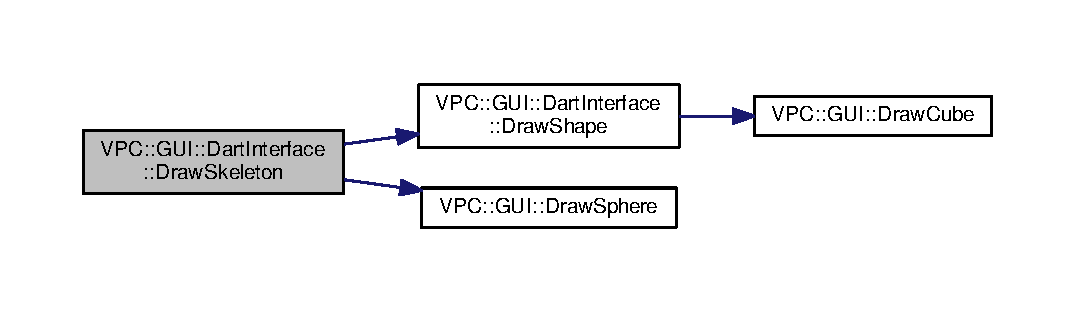
\includegraphics[width=350pt]{namespace_v_p_c_1_1_g_u_i_1_1_dart_interface_a0f48bc6711d69c0979519f00998d1876_cgraph}
\end{center}
\end{figure}




Šeit ir šīs funkcijas izsaukuma grafs\+:
\nopagebreak
\begin{figure}[H]
\begin{center}
\leavevmode
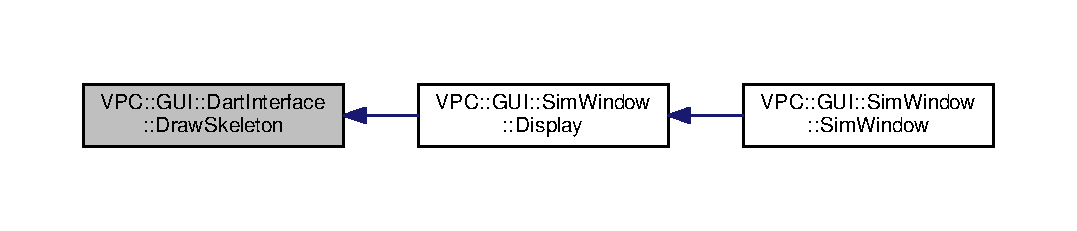
\includegraphics[width=350pt]{namespace_v_p_c_1_1_g_u_i_1_1_dart_interface_a0f48bc6711d69c0979519f00998d1876_icgraph}
\end{center}
\end{figure}



\chapter{Klases dokumentācija}
\hypertarget{classddpg__others_1_1_actor}{}\section{ddpg\+\_\+others.\+Actor klases apraksts}
\label{classddpg__others_1_1_actor}\index{ddpg\+\_\+others.\+Actor@{ddpg\+\_\+others.\+Actor}}


Mantojamības diagramma klasei ddpg\+\_\+others.\+Actor\+:
\nopagebreak
\begin{figure}[H]
\begin{center}
\leavevmode
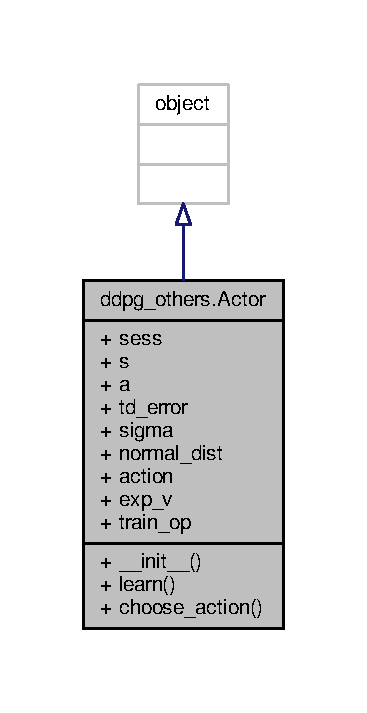
\includegraphics[width=176pt]{classddpg__others_1_1_actor__inherit__graph}
\end{center}
\end{figure}


Sadarbības diagramma klasei ddpg\+\_\+others.\+Actor\+:
\nopagebreak
\begin{figure}[H]
\begin{center}
\leavevmode
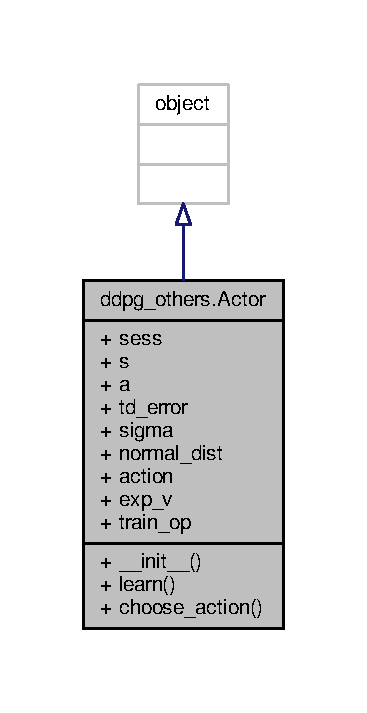
\includegraphics[width=176pt]{classddpg__others_1_1_actor__coll__graph}
\end{center}
\end{figure}
\subsection*{Publiskās elementa funkcijas}
\begin{DoxyCompactItemize}
\item 
def \hyperlink{classddpg__others_1_1_actor_a98635ab068dfa432844a7007d34f923f}{\+\_\+\+\_\+init\+\_\+\+\_\+} (self, \hyperlink{classddpg__others_1_1_actor_af03e8adeb78531e4599419007664842c}{sess}, n\+\_\+features, action\+\_\+bound, lr=0.\+0001)
\item 
def \hyperlink{classddpg__others_1_1_actor_a24e5b40ab12e8d9e6e6eb92385576327}{learn} (self, \hyperlink{classddpg__others_1_1_actor_aa37c0b7d4b4dcc84ab6dd6295a53ef94}{s}, \hyperlink{classddpg__others_1_1_actor_a0f1edbd513cea82df55361aa67ad8794}{a}, td)
\item 
def \hyperlink{classddpg__others_1_1_actor_afef72403fadcc61b70c575d93affd7c1}{choose\+\_\+action} (self, \hyperlink{classddpg__others_1_1_actor_aa37c0b7d4b4dcc84ab6dd6295a53ef94}{s})
\end{DoxyCompactItemize}
\subsection*{Publiskie atribūti}
\begin{DoxyCompactItemize}
\item 
\hyperlink{classddpg__others_1_1_actor_af03e8adeb78531e4599419007664842c}{sess}
\item 
\hyperlink{classddpg__others_1_1_actor_aa37c0b7d4b4dcc84ab6dd6295a53ef94}{s}
\item 
\hyperlink{classddpg__others_1_1_actor_a0f1edbd513cea82df55361aa67ad8794}{a}
\item 
\hyperlink{classddpg__others_1_1_actor_a0b3c557a9af387b1f53279af860d2e57}{td\+\_\+error}
\item 
\hyperlink{classddpg__others_1_1_actor_aed5f0fdc4a7a7ccf996781511f379f29}{sigma}
\item 
\hyperlink{classddpg__others_1_1_actor_a4568b60363c36199737afcb5f7737d8f}{normal\+\_\+dist}
\item 
\hyperlink{classddpg__others_1_1_actor_af0e54cc024b2982a2dea08d5e9091d2b}{action}
\item 
\hyperlink{classddpg__others_1_1_actor_a09356bb2eb8c4b490d6e87ff42e0391d}{exp\+\_\+v}
\item 
\hyperlink{classddpg__others_1_1_actor_a32ca210848490a09496872c1dc69c6a4}{train\+\_\+op}
\end{DoxyCompactItemize}


\subsection{Detalizēts apraksts}


Definēts līnijā 23 failā ddpg\+\_\+others.\+py.



\subsection{Konstruktora un destruktora dokumentācija}
\index{ddpg\+\_\+others\+::\+Actor@{ddpg\+\_\+others\+::\+Actor}!\+\_\+\+\_\+init\+\_\+\+\_\+@{\+\_\+\+\_\+init\+\_\+\+\_\+}}
\index{\+\_\+\+\_\+init\+\_\+\+\_\+@{\+\_\+\+\_\+init\+\_\+\+\_\+}!ddpg\+\_\+others\+::\+Actor@{ddpg\+\_\+others\+::\+Actor}}
\subsubsection[{\texorpdfstring{\+\_\+\+\_\+init\+\_\+\+\_\+(self, sess, n\+\_\+features, action\+\_\+bound, lr=0.\+0001)}{__init__(self, sess, n_features, action_bound, lr=0.0001)}}]{\setlength{\rightskip}{0pt plus 5cm}def ddpg\+\_\+others.\+Actor.\+\_\+\+\_\+init\+\_\+\+\_\+ (
\begin{DoxyParamCaption}
\item[{}]{self, }
\item[{}]{sess, }
\item[{}]{n\+\_\+features, }
\item[{}]{action\+\_\+bound, }
\item[{}]{lr = {\ttfamily 0.0001}}
\end{DoxyParamCaption}
)}\hypertarget{classddpg__others_1_1_actor_a98635ab068dfa432844a7007d34f923f}{}\label{classddpg__others_1_1_actor_a98635ab068dfa432844a7007d34f923f}


Definēts līnijā 24 failā ddpg\+\_\+others.\+py.


\begin{DoxyCode}
24     \textcolor{keyword}{def }\hyperlink{classddpg__others_1_1_actor_a98635ab068dfa432844a7007d34f923f}{\_\_init\_\_}(self, sess, n\_features, action\_bound, lr=0.0001):
25         self.\hyperlink{classddpg__others_1_1_actor_af03e8adeb78531e4599419007664842c}{sess} = sess
26 
27         self.\hyperlink{classddpg__others_1_1_actor_aa37c0b7d4b4dcc84ab6dd6295a53ef94}{s} = tf.placeholder(tf.float32, [1, n\_features], \textcolor{stringliteral}{"state"})
28         self.\hyperlink{classddpg__others_1_1_actor_a0f1edbd513cea82df55361aa67ad8794}{a} = tf.placeholder(tf.float32, \textcolor{keywordtype}{None}, name=\textcolor{stringliteral}{"act"})
29         self.\hyperlink{classddpg__others_1_1_actor_a0b3c557a9af387b1f53279af860d2e57}{td\_error} = tf.placeholder(tf.float32, \textcolor{keywordtype}{None}, name=\textcolor{stringliteral}{"td\_error"})  \textcolor{comment}{# TD\_error}
30 
31         l1 = tf.layers.dense(
32             inputs=self.\hyperlink{classddpg__others_1_1_actor_aa37c0b7d4b4dcc84ab6dd6295a53ef94}{s},
33             units=30,  \textcolor{comment}{# number of hidden units}
34             activation=tf.nn.relu,
35             kernel\_initializer=tf.random\_normal\_initializer(0., .1),  \textcolor{comment}{# weights}
36             bias\_initializer=tf.constant\_initializer(0.1),  \textcolor{comment}{# biases}
37             name=\textcolor{stringliteral}{'l1'}
38         )
39 
40         mu = tf.layers.dense(
41             inputs=l1,
42             units=1,  \textcolor{comment}{# number of hidden units}
43             activation=tf.nn.tanh,
44             kernel\_initializer=tf.random\_normal\_initializer(0., .1),  \textcolor{comment}{# weights}
45             bias\_initializer=tf.constant\_initializer(0.1),  \textcolor{comment}{# biases}
46             name=\textcolor{stringliteral}{'mu'}
47         )
48 
49         sigma = tf.layers.dense(
50             inputs=l1,
51             units=1,  \textcolor{comment}{# output units}
52             activation=tf.nn.softplus,  \textcolor{comment}{# get action probabilities}
53             kernel\_initializer=tf.random\_normal\_initializer(0., .1),  \textcolor{comment}{# weights}
54             bias\_initializer=tf.constant\_initializer(1.),  \textcolor{comment}{# biases}
55             name=\textcolor{stringliteral}{'sigma'}
56         )
57         global\_step = tf.Variable(0, trainable=\textcolor{keyword}{False})
58         \textcolor{comment}{# self.e = epsilon = tf.train.exponential\_decay(2., global\_step, 1000, 0.9)}
59         self.mu, self.\hyperlink{classddpg__others_1_1_actor_aed5f0fdc4a7a7ccf996781511f379f29}{sigma} = tf.squeeze(mu*2), tf.squeeze(sigma+0.1)
60         self.\hyperlink{classddpg__others_1_1_actor_a4568b60363c36199737afcb5f7737d8f}{normal\_dist} = tf.distributions.Normal(self.mu, self.
      \hyperlink{classddpg__others_1_1_actor_aed5f0fdc4a7a7ccf996781511f379f29}{sigma})
61 
62         self.\hyperlink{classddpg__others_1_1_actor_af0e54cc024b2982a2dea08d5e9091d2b}{action} = tf.clip\_by\_value(self.normal\_dist.sample(1), action\_bound[0], action\_bound[1])
63 
64         with tf.name\_scope(\textcolor{stringliteral}{'exp\_v'}):
65             log\_prob = self.normal\_dist.log\_prob(self.\hyperlink{classddpg__others_1_1_actor_a0f1edbd513cea82df55361aa67ad8794}{a})  \textcolor{comment}{# loss without advantage}
66             self.\hyperlink{classddpg__others_1_1_actor_a09356bb2eb8c4b490d6e87ff42e0391d}{exp\_v} = log\_prob * self.\hyperlink{classddpg__others_1_1_actor_a0b3c557a9af387b1f53279af860d2e57}{td\_error}  \textcolor{comment}{# advantage (TD\_error) guided loss}
67             \textcolor{comment}{# Add cross entropy cost to encourage exploration}
68             self.\hyperlink{classddpg__others_1_1_actor_a09356bb2eb8c4b490d6e87ff42e0391d}{exp\_v} += 0.01*self.normal\_dist.entropy()
69 
70         with tf.name\_scope(\textcolor{stringliteral}{'train'}):
71             self.\hyperlink{classddpg__others_1_1_actor_a32ca210848490a09496872c1dc69c6a4}{train\_op} = tf.train.AdamOptimizer(lr).minimize(-self.
      \hyperlink{classddpg__others_1_1_actor_a09356bb2eb8c4b490d6e87ff42e0391d}{exp\_v}, global\_step)    \textcolor{comment}{# min(v) = max(-v)}
72 
\end{DoxyCode}


\subsection{Elementa funkcijas dokumentācija}
\index{ddpg\+\_\+others\+::\+Actor@{ddpg\+\_\+others\+::\+Actor}!choose\+\_\+action@{choose\+\_\+action}}
\index{choose\+\_\+action@{choose\+\_\+action}!ddpg\+\_\+others\+::\+Actor@{ddpg\+\_\+others\+::\+Actor}}
\subsubsection[{\texorpdfstring{choose\+\_\+action(self, s)}{choose_action(self, s)}}]{\setlength{\rightskip}{0pt plus 5cm}def ddpg\+\_\+others.\+Actor.\+choose\+\_\+action (
\begin{DoxyParamCaption}
\item[{}]{self, }
\item[{}]{s}
\end{DoxyParamCaption}
)}\hypertarget{classddpg__others_1_1_actor_afef72403fadcc61b70c575d93affd7c1}{}\label{classddpg__others_1_1_actor_afef72403fadcc61b70c575d93affd7c1}


Definēts līnijā 79 failā ddpg\+\_\+others.\+py.


\begin{DoxyCode}
79     \textcolor{keyword}{def }\hyperlink{classddpg__others_1_1_actor_afef72403fadcc61b70c575d93affd7c1}{choose\_action}(self, s):
80         s = s[np.newaxis, :]
81         \textcolor{keywordflow}{return} self.sess.run(self.\hyperlink{classddpg__others_1_1_actor_af0e54cc024b2982a2dea08d5e9091d2b}{action}, \{self.\hyperlink{classddpg__others_1_1_actor_aa37c0b7d4b4dcc84ab6dd6295a53ef94}{s}: s\})  \textcolor{comment}{# get probabilities for all actions}
82 
83 
\end{DoxyCode}
\index{ddpg\+\_\+others\+::\+Actor@{ddpg\+\_\+others\+::\+Actor}!learn@{learn}}
\index{learn@{learn}!ddpg\+\_\+others\+::\+Actor@{ddpg\+\_\+others\+::\+Actor}}
\subsubsection[{\texorpdfstring{learn(self, s, a, td)}{learn(self, s, a, td)}}]{\setlength{\rightskip}{0pt plus 5cm}def ddpg\+\_\+others.\+Actor.\+learn (
\begin{DoxyParamCaption}
\item[{}]{self, }
\item[{}]{s, }
\item[{}]{a, }
\item[{}]{td}
\end{DoxyParamCaption}
)}\hypertarget{classddpg__others_1_1_actor_a24e5b40ab12e8d9e6e6eb92385576327}{}\label{classddpg__others_1_1_actor_a24e5b40ab12e8d9e6e6eb92385576327}


Definēts līnijā 73 failā ddpg\+\_\+others.\+py.


\begin{DoxyCode}
73     \textcolor{keyword}{def }\hyperlink{classddpg__others_1_1_actor_a24e5b40ab12e8d9e6e6eb92385576327}{learn}(self, s, a, td):
74         s = s[np.newaxis, :]
75         feed\_dict = \{self.\hyperlink{classddpg__others_1_1_actor_aa37c0b7d4b4dcc84ab6dd6295a53ef94}{s}: s, self.\hyperlink{classddpg__others_1_1_actor_a0f1edbd513cea82df55361aa67ad8794}{a}: a, self.\hyperlink{classddpg__others_1_1_actor_a0b3c557a9af387b1f53279af860d2e57}{td\_error}: td\}
76         \_, exp\_v = self.sess.run([self.\hyperlink{classddpg__others_1_1_actor_a32ca210848490a09496872c1dc69c6a4}{train\_op}, self.\hyperlink{classddpg__others_1_1_actor_a09356bb2eb8c4b490d6e87ff42e0391d}{exp\_v}], feed\_dict)
77         \textcolor{keywordflow}{return} exp\_v
78 
\end{DoxyCode}


\subsection{Elementa datu dokumentācija}
\index{ddpg\+\_\+others\+::\+Actor@{ddpg\+\_\+others\+::\+Actor}!a@{a}}
\index{a@{a}!ddpg\+\_\+others\+::\+Actor@{ddpg\+\_\+others\+::\+Actor}}
\subsubsection[{\texorpdfstring{a}{a}}]{\setlength{\rightskip}{0pt plus 5cm}ddpg\+\_\+others.\+Actor.\+a}\hypertarget{classddpg__others_1_1_actor_a0f1edbd513cea82df55361aa67ad8794}{}\label{classddpg__others_1_1_actor_a0f1edbd513cea82df55361aa67ad8794}


Definēts līnijā 28 failā ddpg\+\_\+others.\+py.

\index{ddpg\+\_\+others\+::\+Actor@{ddpg\+\_\+others\+::\+Actor}!action@{action}}
\index{action@{action}!ddpg\+\_\+others\+::\+Actor@{ddpg\+\_\+others\+::\+Actor}}
\subsubsection[{\texorpdfstring{action}{action}}]{\setlength{\rightskip}{0pt plus 5cm}ddpg\+\_\+others.\+Actor.\+action}\hypertarget{classddpg__others_1_1_actor_af0e54cc024b2982a2dea08d5e9091d2b}{}\label{classddpg__others_1_1_actor_af0e54cc024b2982a2dea08d5e9091d2b}


Definēts līnijā 62 failā ddpg\+\_\+others.\+py.

\index{ddpg\+\_\+others\+::\+Actor@{ddpg\+\_\+others\+::\+Actor}!exp\+\_\+v@{exp\+\_\+v}}
\index{exp\+\_\+v@{exp\+\_\+v}!ddpg\+\_\+others\+::\+Actor@{ddpg\+\_\+others\+::\+Actor}}
\subsubsection[{\texorpdfstring{exp\+\_\+v}{exp_v}}]{\setlength{\rightskip}{0pt plus 5cm}ddpg\+\_\+others.\+Actor.\+exp\+\_\+v}\hypertarget{classddpg__others_1_1_actor_a09356bb2eb8c4b490d6e87ff42e0391d}{}\label{classddpg__others_1_1_actor_a09356bb2eb8c4b490d6e87ff42e0391d}


Definēts līnijā 66 failā ddpg\+\_\+others.\+py.

\index{ddpg\+\_\+others\+::\+Actor@{ddpg\+\_\+others\+::\+Actor}!normal\+\_\+dist@{normal\+\_\+dist}}
\index{normal\+\_\+dist@{normal\+\_\+dist}!ddpg\+\_\+others\+::\+Actor@{ddpg\+\_\+others\+::\+Actor}}
\subsubsection[{\texorpdfstring{normal\+\_\+dist}{normal_dist}}]{\setlength{\rightskip}{0pt plus 5cm}ddpg\+\_\+others.\+Actor.\+normal\+\_\+dist}\hypertarget{classddpg__others_1_1_actor_a4568b60363c36199737afcb5f7737d8f}{}\label{classddpg__others_1_1_actor_a4568b60363c36199737afcb5f7737d8f}


Definēts līnijā 60 failā ddpg\+\_\+others.\+py.

\index{ddpg\+\_\+others\+::\+Actor@{ddpg\+\_\+others\+::\+Actor}!s@{s}}
\index{s@{s}!ddpg\+\_\+others\+::\+Actor@{ddpg\+\_\+others\+::\+Actor}}
\subsubsection[{\texorpdfstring{s}{s}}]{\setlength{\rightskip}{0pt plus 5cm}ddpg\+\_\+others.\+Actor.\+s}\hypertarget{classddpg__others_1_1_actor_aa37c0b7d4b4dcc84ab6dd6295a53ef94}{}\label{classddpg__others_1_1_actor_aa37c0b7d4b4dcc84ab6dd6295a53ef94}


Definēts līnijā 27 failā ddpg\+\_\+others.\+py.

\index{ddpg\+\_\+others\+::\+Actor@{ddpg\+\_\+others\+::\+Actor}!sess@{sess}}
\index{sess@{sess}!ddpg\+\_\+others\+::\+Actor@{ddpg\+\_\+others\+::\+Actor}}
\subsubsection[{\texorpdfstring{sess}{sess}}]{\setlength{\rightskip}{0pt plus 5cm}ddpg\+\_\+others.\+Actor.\+sess}\hypertarget{classddpg__others_1_1_actor_af03e8adeb78531e4599419007664842c}{}\label{classddpg__others_1_1_actor_af03e8adeb78531e4599419007664842c}


Definēts līnijā 25 failā ddpg\+\_\+others.\+py.

\index{ddpg\+\_\+others\+::\+Actor@{ddpg\+\_\+others\+::\+Actor}!sigma@{sigma}}
\index{sigma@{sigma}!ddpg\+\_\+others\+::\+Actor@{ddpg\+\_\+others\+::\+Actor}}
\subsubsection[{\texorpdfstring{sigma}{sigma}}]{\setlength{\rightskip}{0pt plus 5cm}ddpg\+\_\+others.\+Actor.\+sigma}\hypertarget{classddpg__others_1_1_actor_aed5f0fdc4a7a7ccf996781511f379f29}{}\label{classddpg__others_1_1_actor_aed5f0fdc4a7a7ccf996781511f379f29}


Definēts līnijā 59 failā ddpg\+\_\+others.\+py.

\index{ddpg\+\_\+others\+::\+Actor@{ddpg\+\_\+others\+::\+Actor}!td\+\_\+error@{td\+\_\+error}}
\index{td\+\_\+error@{td\+\_\+error}!ddpg\+\_\+others\+::\+Actor@{ddpg\+\_\+others\+::\+Actor}}
\subsubsection[{\texorpdfstring{td\+\_\+error}{td_error}}]{\setlength{\rightskip}{0pt plus 5cm}ddpg\+\_\+others.\+Actor.\+td\+\_\+error}\hypertarget{classddpg__others_1_1_actor_a0b3c557a9af387b1f53279af860d2e57}{}\label{classddpg__others_1_1_actor_a0b3c557a9af387b1f53279af860d2e57}


Definēts līnijā 29 failā ddpg\+\_\+others.\+py.

\index{ddpg\+\_\+others\+::\+Actor@{ddpg\+\_\+others\+::\+Actor}!train\+\_\+op@{train\+\_\+op}}
\index{train\+\_\+op@{train\+\_\+op}!ddpg\+\_\+others\+::\+Actor@{ddpg\+\_\+others\+::\+Actor}}
\subsubsection[{\texorpdfstring{train\+\_\+op}{train_op}}]{\setlength{\rightskip}{0pt plus 5cm}ddpg\+\_\+others.\+Actor.\+train\+\_\+op}\hypertarget{classddpg__others_1_1_actor_a32ca210848490a09496872c1dc69c6a4}{}\label{classddpg__others_1_1_actor_a32ca210848490a09496872c1dc69c6a4}


Definēts līnijā 71 failā ddpg\+\_\+others.\+py.



Šīs klases dokumentācijas tika ģenerēta no šāda faila\+:\begin{DoxyCompactItemize}
\item 
py\+\_\+code/\hyperlink{ddpg__others_8py}{ddpg\+\_\+others.\+py}\end{DoxyCompactItemize}

\hypertarget{classactor_1_1_actor_network}{}\section{actor.\+Actor\+Network klases apraksts}
\label{classactor_1_1_actor_network}\index{actor.\+Actor\+Network@{actor.\+Actor\+Network}}


Sadarbības diagramma klasei actor.\+Actor\+Network\+:
\nopagebreak
\begin{figure}[H]
\begin{center}
\leavevmode
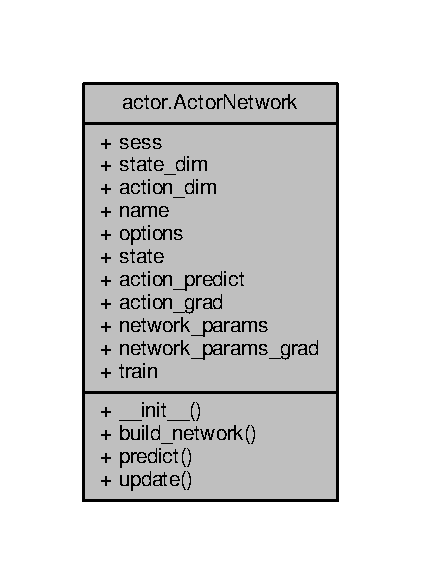
\includegraphics[width=202pt]{classactor_1_1_actor_network__coll__graph}
\end{center}
\end{figure}
\subsection*{Publiskās elementa funkcijas}
\begin{DoxyCompactItemize}
\item 
def \hyperlink{classactor_1_1_actor_network_a4fc65628c69ee1807e95af77b6794046}{\+\_\+\+\_\+init\+\_\+\+\_\+} (self, \hyperlink{classactor_1_1_actor_network_ae8daea79f8d1f754c3d44c76036da21a}{sess}, \hyperlink{classactor_1_1_actor_network_af7cdb447ae7a2a605a9a22336297d34f}{options}, \hyperlink{classactor_1_1_actor_network_adecdbb6d5d6d12f4c9d36b22bd9ad6c4}{name})
\item 
def \hyperlink{classactor_1_1_actor_network_acf991872a87f6ba32f828e6611262a1b}{build\+\_\+network} (self)
\item 
def \hyperlink{classactor_1_1_actor_network_add9742704ce6dbd77bd645e9ee9f4ed5}{predict} (self, \hyperlink{classactor_1_1_actor_network_ab3bae8f52b46f6b7ee7c9f4f0cd21c45}{state})
\item 
def \hyperlink{classactor_1_1_actor_network_a730e1fa368e30085d1f320b99afa5571}{update} (self, states, action\+\_\+grads)
\end{DoxyCompactItemize}
\subsection*{Publiskie atribūti}
\begin{DoxyCompactItemize}
\item 
\hyperlink{classactor_1_1_actor_network_ae8daea79f8d1f754c3d44c76036da21a}{sess}
\item 
\hyperlink{classactor_1_1_actor_network_a5a97fa085ad81efe114122af1cff8d26}{state\+\_\+dim}
\item 
\hyperlink{classactor_1_1_actor_network_ada197a9b6d5e1b5ebcdcc360d11e4f1b}{action\+\_\+dim}
\item 
\hyperlink{classactor_1_1_actor_network_adecdbb6d5d6d12f4c9d36b22bd9ad6c4}{name}
\item 
\hyperlink{classactor_1_1_actor_network_af7cdb447ae7a2a605a9a22336297d34f}{options}
\item 
\hyperlink{classactor_1_1_actor_network_ab3bae8f52b46f6b7ee7c9f4f0cd21c45}{state}
\item 
\hyperlink{classactor_1_1_actor_network_a8cbb128a36aa9bc9279880c34d503af3}{action\+\_\+predict}
\item 
\hyperlink{classactor_1_1_actor_network_a1420ab0da00328629de6fe8087c4c4e7}{action\+\_\+grad}
\item 
\hyperlink{classactor_1_1_actor_network_ae0bac8c1fdcbdf33f9651444e66f9e09}{network\+\_\+params}
\item 
\hyperlink{classactor_1_1_actor_network_ae6932b19d7a23205226ab1bc454a5693}{network\+\_\+params\+\_\+grad}
\item 
\hyperlink{classactor_1_1_actor_network_a10e3ddfa0963a82bec05f3a0fa59d023}{train}
\end{DoxyCompactItemize}


\subsection{Detalizēts apraksts}


Definēts līnijā 4 failā actor.\+py.



\subsection{Konstruktora un destruktora dokumentācija}
\index{actor\+::\+Actor\+Network@{actor\+::\+Actor\+Network}!\+\_\+\+\_\+init\+\_\+\+\_\+@{\+\_\+\+\_\+init\+\_\+\+\_\+}}
\index{\+\_\+\+\_\+init\+\_\+\+\_\+@{\+\_\+\+\_\+init\+\_\+\+\_\+}!actor\+::\+Actor\+Network@{actor\+::\+Actor\+Network}}
\subsubsection[{\texorpdfstring{\+\_\+\+\_\+init\+\_\+\+\_\+(self, sess, options, name)}{__init__(self, sess, options, name)}}]{\setlength{\rightskip}{0pt plus 5cm}def actor.\+Actor\+Network.\+\_\+\+\_\+init\+\_\+\+\_\+ (
\begin{DoxyParamCaption}
\item[{}]{self, }
\item[{}]{sess, }
\item[{}]{options, }
\item[{}]{name}
\end{DoxyParamCaption}
)}\hypertarget{classactor_1_1_actor_network_a4fc65628c69ee1807e95af77b6794046}{}\label{classactor_1_1_actor_network_a4fc65628c69ee1807e95af77b6794046}


Definēts līnijā 5 failā actor.\+py.


\begin{DoxyCode}
5     \textcolor{keyword}{def }\hyperlink{classactor_1_1_actor_network_a4fc65628c69ee1807e95af77b6794046}{\_\_init\_\_}(self,sess,options,name):
6         \textcolor{comment}{# session}
7         \textcolor{comment}{# state\_dim}
8         \textcolor{comment}{# action\_dim}
9         \textcolor{comment}{# learning\_rate}
10         \textcolor{comment}{# name}
11         self.\hyperlink{classactor_1_1_actor_network_ae8daea79f8d1f754c3d44c76036da21a}{sess} = sess
12         self.\hyperlink{classactor_1_1_actor_network_a5a97fa085ad81efe114122af1cff8d26}{state\_dim} = options.STATE\_DIM
13         self.\hyperlink{classactor_1_1_actor_network_ada197a9b6d5e1b5ebcdcc360d11e4f1b}{action\_dim} = options.ACTION\_DIM
14         self.\hyperlink{classactor_1_1_actor_network_adecdbb6d5d6d12f4c9d36b22bd9ad6c4}{name} = name
15         self.\hyperlink{classactor_1_1_actor_network_af7cdb447ae7a2a605a9a22336297d34f}{options} = options
16 
17         self.\hyperlink{classactor_1_1_actor_network_acf991872a87f6ba32f828e6611262a1b}{build\_network}()
18 
19         init\_vars = tf.group(tf.global\_variables\_initializer(), tf.local\_variables\_initializer())
20         sess.run(init\_vars)
21 
\end{DoxyCode}


\subsection{Elementa funkcijas dokumentācija}
\index{actor\+::\+Actor\+Network@{actor\+::\+Actor\+Network}!build\+\_\+network@{build\+\_\+network}}
\index{build\+\_\+network@{build\+\_\+network}!actor\+::\+Actor\+Network@{actor\+::\+Actor\+Network}}
\subsubsection[{\texorpdfstring{build\+\_\+network(self)}{build_network(self)}}]{\setlength{\rightskip}{0pt plus 5cm}def actor.\+Actor\+Network.\+build\+\_\+network (
\begin{DoxyParamCaption}
\item[{}]{self}
\end{DoxyParamCaption}
)}\hypertarget{classactor_1_1_actor_network_acf991872a87f6ba32f828e6611262a1b}{}\label{classactor_1_1_actor_network_acf991872a87f6ba32f828e6611262a1b}


Definēts līnijā 23 failā actor.\+py.


\begin{DoxyCode}
23     \textcolor{keyword}{def }\hyperlink{classactor_1_1_actor_network_acf991872a87f6ba32f828e6611262a1b}{build\_network}(self):
24         self.\hyperlink{classactor_1_1_actor_network_ab3bae8f52b46f6b7ee7c9f4f0cd21c45}{state} = tf.placeholder(tf.float32, [\textcolor{keywordtype}{None}, self.\hyperlink{classactor_1_1_actor_network_a5a97fa085ad81efe114122af1cff8d26}{state\_dim}]) \textcolor{comment}{# Placeholder}
25         with tf.variable\_scope(self.\hyperlink{classactor_1_1_actor_network_adecdbb6d5d6d12f4c9d36b22bd9ad6c4}{name}):
26             hidden\_layer = tf.layers.dense(self.\hyperlink{classactor_1_1_actor_network_ab3bae8f52b46f6b7ee7c9f4f0cd21c45}{state}, 64, activation = tf.nn.elu, kernel\_initializer 
      = tf.contrib.layers.xavier\_initializer()) \textcolor{comment}{# use elu for hidden layer}
27             self.\hyperlink{classactor_1_1_actor_network_a8cbb128a36aa9bc9279880c34d503af3}{action\_predict} = tf.layers.dense(hidden\_layer, self.
      \hyperlink{classactor_1_1_actor_network_ada197a9b6d5e1b5ebcdcc360d11e4f1b}{action\_dim}, activation = tf.nn.tanh, kernel\_initializer = tf.contrib.layers.xavier\_initializer())
       \textcolor{comment}{# use tanh to ensure output range becomes [-1,1]}
28 
29         self.\hyperlink{classactor_1_1_actor_network_a1420ab0da00328629de6fe8087c4c4e7}{action\_grad} = tf.placeholder(tf.float32, [\textcolor{keywordtype}{None}, self.
      \hyperlink{classactor_1_1_actor_network_ada197a9b6d5e1b5ebcdcc360d11e4f1b}{action\_dim}]) \textcolor{comment}{# Placeholder}
30         self.\hyperlink{classactor_1_1_actor_network_ae0bac8c1fdcbdf33f9651444e66f9e09}{network\_params} = tf.trainable\_variables(scope = self.
      \hyperlink{classactor_1_1_actor_network_adecdbb6d5d6d12f4c9d36b22bd9ad6c4}{name})
31 
32         \textcolor{comment}{# find d(xs) s.t. d(ys)=grad\_ys}
33         \textcolor{comment}{# since grad\_ys is given, result is gradient of each network params for satisfying given grad\_ys}
34         \textcolor{comment}{# in other word, net params should be changed as net\_params\_grad to change ys as grad\_ys}
35         self.\hyperlink{classactor_1_1_actor_network_ae6932b19d7a23205226ab1bc454a5693}{network\_params\_grad} = tf.gradients(ys=self.
      \hyperlink{classactor_1_1_actor_network_a8cbb128a36aa9bc9279880c34d503af3}{action\_predict}, xs=self.\hyperlink{classactor_1_1_actor_network_ae0bac8c1fdcbdf33f9651444e66f9e09}{network\_params}, grad\_ys=-self.
      \hyperlink{classactor_1_1_actor_network_a1420ab0da00328629de6fe8087c4c4e7}{action\_grad})
36 
37         \textcolor{comment}{# train}
38         self.\hyperlink{classactor_1_1_actor_network_a10e3ddfa0963a82bec05f3a0fa59d023}{train} = tf.train.AdamOptimizer(self.options.LR\_A).apply\_gradients(zip(self.
      \hyperlink{classactor_1_1_actor_network_ae6932b19d7a23205226ab1bc454a5693}{network\_params\_grad}, self.\hyperlink{classactor_1_1_actor_network_ae0bac8c1fdcbdf33f9651444e66f9e09}{network\_params}))
39 
\end{DoxyCode}
\index{actor\+::\+Actor\+Network@{actor\+::\+Actor\+Network}!predict@{predict}}
\index{predict@{predict}!actor\+::\+Actor\+Network@{actor\+::\+Actor\+Network}}
\subsubsection[{\texorpdfstring{predict(self, state)}{predict(self, state)}}]{\setlength{\rightskip}{0pt plus 5cm}def actor.\+Actor\+Network.\+predict (
\begin{DoxyParamCaption}
\item[{}]{self, }
\item[{}]{state}
\end{DoxyParamCaption}
)}\hypertarget{classactor_1_1_actor_network_add9742704ce6dbd77bd645e9ee9f4ed5}{}\label{classactor_1_1_actor_network_add9742704ce6dbd77bd645e9ee9f4ed5}


Definēts līnijā 40 failā actor.\+py.


\begin{DoxyCode}
40     \textcolor{keyword}{def }\hyperlink{classactor_1_1_actor_network_add9742704ce6dbd77bd645e9ee9f4ed5}{predict}(self, state):
41         s = np.reshape(state, [-1, self.\hyperlink{classactor_1_1_actor_network_a5a97fa085ad81efe114122af1cff8d26}{state\_dim}]) \textcolor{comment}{# ensure right shape}
42         \textcolor{keywordflow}{return} self.sess.run(self.\hyperlink{classactor_1_1_actor_network_a8cbb128a36aa9bc9279880c34d503af3}{action\_predict},
43                              feed\_dict=\{
44                                  self.\hyperlink{classactor_1_1_actor_network_ab3bae8f52b46f6b7ee7c9f4f0cd21c45}{state} : s
45                              \})
46 
47 
\end{DoxyCode}
\index{actor\+::\+Actor\+Network@{actor\+::\+Actor\+Network}!update@{update}}
\index{update@{update}!actor\+::\+Actor\+Network@{actor\+::\+Actor\+Network}}
\subsubsection[{\texorpdfstring{update(self, states, action\+\_\+grads)}{update(self, states, action_grads)}}]{\setlength{\rightskip}{0pt plus 5cm}def actor.\+Actor\+Network.\+update (
\begin{DoxyParamCaption}
\item[{}]{self, }
\item[{}]{states, }
\item[{}]{action\+\_\+grads}
\end{DoxyParamCaption}
)}\hypertarget{classactor_1_1_actor_network_a730e1fa368e30085d1f320b99afa5571}{}\label{classactor_1_1_actor_network_a730e1fa368e30085d1f320b99afa5571}


Definēts līnijā 48 failā actor.\+py.


\begin{DoxyCode}
48     \textcolor{keyword}{def }\hyperlink{classactor_1_1_actor_network_a730e1fa368e30085d1f320b99afa5571}{update}(self, states, action\_grads):
49         self.sess.run(self.\hyperlink{classactor_1_1_actor_network_a10e3ddfa0963a82bec05f3a0fa59d023}{train},
50                       feed\_dict=\{
51                           self.\hyperlink{classactor_1_1_actor_network_ab3bae8f52b46f6b7ee7c9f4f0cd21c45}{state}: states,
52                           self.\hyperlink{classactor_1_1_actor_network_a1420ab0da00328629de6fe8087c4c4e7}{action\_grad}: action\_grads
53                       \}\end{DoxyCode}


\subsection{Elementa datu dokumentācija}
\index{actor\+::\+Actor\+Network@{actor\+::\+Actor\+Network}!action\+\_\+dim@{action\+\_\+dim}}
\index{action\+\_\+dim@{action\+\_\+dim}!actor\+::\+Actor\+Network@{actor\+::\+Actor\+Network}}
\subsubsection[{\texorpdfstring{action\+\_\+dim}{action_dim}}]{\setlength{\rightskip}{0pt plus 5cm}actor.\+Actor\+Network.\+action\+\_\+dim}\hypertarget{classactor_1_1_actor_network_ada197a9b6d5e1b5ebcdcc360d11e4f1b}{}\label{classactor_1_1_actor_network_ada197a9b6d5e1b5ebcdcc360d11e4f1b}


Definēts līnijā 13 failā actor.\+py.

\index{actor\+::\+Actor\+Network@{actor\+::\+Actor\+Network}!action\+\_\+grad@{action\+\_\+grad}}
\index{action\+\_\+grad@{action\+\_\+grad}!actor\+::\+Actor\+Network@{actor\+::\+Actor\+Network}}
\subsubsection[{\texorpdfstring{action\+\_\+grad}{action_grad}}]{\setlength{\rightskip}{0pt plus 5cm}actor.\+Actor\+Network.\+action\+\_\+grad}\hypertarget{classactor_1_1_actor_network_a1420ab0da00328629de6fe8087c4c4e7}{}\label{classactor_1_1_actor_network_a1420ab0da00328629de6fe8087c4c4e7}


Definēts līnijā 29 failā actor.\+py.

\index{actor\+::\+Actor\+Network@{actor\+::\+Actor\+Network}!action\+\_\+predict@{action\+\_\+predict}}
\index{action\+\_\+predict@{action\+\_\+predict}!actor\+::\+Actor\+Network@{actor\+::\+Actor\+Network}}
\subsubsection[{\texorpdfstring{action\+\_\+predict}{action_predict}}]{\setlength{\rightskip}{0pt plus 5cm}actor.\+Actor\+Network.\+action\+\_\+predict}\hypertarget{classactor_1_1_actor_network_a8cbb128a36aa9bc9279880c34d503af3}{}\label{classactor_1_1_actor_network_a8cbb128a36aa9bc9279880c34d503af3}


Definēts līnijā 27 failā actor.\+py.

\index{actor\+::\+Actor\+Network@{actor\+::\+Actor\+Network}!name@{name}}
\index{name@{name}!actor\+::\+Actor\+Network@{actor\+::\+Actor\+Network}}
\subsubsection[{\texorpdfstring{name}{name}}]{\setlength{\rightskip}{0pt plus 5cm}actor.\+Actor\+Network.\+name}\hypertarget{classactor_1_1_actor_network_adecdbb6d5d6d12f4c9d36b22bd9ad6c4}{}\label{classactor_1_1_actor_network_adecdbb6d5d6d12f4c9d36b22bd9ad6c4}


Definēts līnijā 14 failā actor.\+py.

\index{actor\+::\+Actor\+Network@{actor\+::\+Actor\+Network}!network\+\_\+params@{network\+\_\+params}}
\index{network\+\_\+params@{network\+\_\+params}!actor\+::\+Actor\+Network@{actor\+::\+Actor\+Network}}
\subsubsection[{\texorpdfstring{network\+\_\+params}{network_params}}]{\setlength{\rightskip}{0pt plus 5cm}actor.\+Actor\+Network.\+network\+\_\+params}\hypertarget{classactor_1_1_actor_network_ae0bac8c1fdcbdf33f9651444e66f9e09}{}\label{classactor_1_1_actor_network_ae0bac8c1fdcbdf33f9651444e66f9e09}


Definēts līnijā 30 failā actor.\+py.

\index{actor\+::\+Actor\+Network@{actor\+::\+Actor\+Network}!network\+\_\+params\+\_\+grad@{network\+\_\+params\+\_\+grad}}
\index{network\+\_\+params\+\_\+grad@{network\+\_\+params\+\_\+grad}!actor\+::\+Actor\+Network@{actor\+::\+Actor\+Network}}
\subsubsection[{\texorpdfstring{network\+\_\+params\+\_\+grad}{network_params_grad}}]{\setlength{\rightskip}{0pt plus 5cm}actor.\+Actor\+Network.\+network\+\_\+params\+\_\+grad}\hypertarget{classactor_1_1_actor_network_ae6932b19d7a23205226ab1bc454a5693}{}\label{classactor_1_1_actor_network_ae6932b19d7a23205226ab1bc454a5693}


Definēts līnijā 35 failā actor.\+py.

\index{actor\+::\+Actor\+Network@{actor\+::\+Actor\+Network}!options@{options}}
\index{options@{options}!actor\+::\+Actor\+Network@{actor\+::\+Actor\+Network}}
\subsubsection[{\texorpdfstring{options}{options}}]{\setlength{\rightskip}{0pt plus 5cm}actor.\+Actor\+Network.\+options}\hypertarget{classactor_1_1_actor_network_af7cdb447ae7a2a605a9a22336297d34f}{}\label{classactor_1_1_actor_network_af7cdb447ae7a2a605a9a22336297d34f}


Definēts līnijā 15 failā actor.\+py.

\index{actor\+::\+Actor\+Network@{actor\+::\+Actor\+Network}!sess@{sess}}
\index{sess@{sess}!actor\+::\+Actor\+Network@{actor\+::\+Actor\+Network}}
\subsubsection[{\texorpdfstring{sess}{sess}}]{\setlength{\rightskip}{0pt plus 5cm}actor.\+Actor\+Network.\+sess}\hypertarget{classactor_1_1_actor_network_ae8daea79f8d1f754c3d44c76036da21a}{}\label{classactor_1_1_actor_network_ae8daea79f8d1f754c3d44c76036da21a}


Definēts līnijā 11 failā actor.\+py.

\index{actor\+::\+Actor\+Network@{actor\+::\+Actor\+Network}!state@{state}}
\index{state@{state}!actor\+::\+Actor\+Network@{actor\+::\+Actor\+Network}}
\subsubsection[{\texorpdfstring{state}{state}}]{\setlength{\rightskip}{0pt plus 5cm}actor.\+Actor\+Network.\+state}\hypertarget{classactor_1_1_actor_network_ab3bae8f52b46f6b7ee7c9f4f0cd21c45}{}\label{classactor_1_1_actor_network_ab3bae8f52b46f6b7ee7c9f4f0cd21c45}


Definēts līnijā 24 failā actor.\+py.

\index{actor\+::\+Actor\+Network@{actor\+::\+Actor\+Network}!state\+\_\+dim@{state\+\_\+dim}}
\index{state\+\_\+dim@{state\+\_\+dim}!actor\+::\+Actor\+Network@{actor\+::\+Actor\+Network}}
\subsubsection[{\texorpdfstring{state\+\_\+dim}{state_dim}}]{\setlength{\rightskip}{0pt plus 5cm}actor.\+Actor\+Network.\+state\+\_\+dim}\hypertarget{classactor_1_1_actor_network_a5a97fa085ad81efe114122af1cff8d26}{}\label{classactor_1_1_actor_network_a5a97fa085ad81efe114122af1cff8d26}


Definēts līnijā 12 failā actor.\+py.

\index{actor\+::\+Actor\+Network@{actor\+::\+Actor\+Network}!train@{train}}
\index{train@{train}!actor\+::\+Actor\+Network@{actor\+::\+Actor\+Network}}
\subsubsection[{\texorpdfstring{train}{train}}]{\setlength{\rightskip}{0pt plus 5cm}actor.\+Actor\+Network.\+train}\hypertarget{classactor_1_1_actor_network_a10e3ddfa0963a82bec05f3a0fa59d023}{}\label{classactor_1_1_actor_network_a10e3ddfa0963a82bec05f3a0fa59d023}


Definēts līnijā 38 failā actor.\+py.



Šīs klases dokumentācijas tika ģenerēta no šāda faila\+:\begin{DoxyCompactItemize}
\item 
py\+\_\+code/\hyperlink{actor_8py}{actor.\+py}\end{DoxyCompactItemize}

\hypertarget{class_v_p_c_1_1_g_u_i_1_1_camera}{}\section{V\+PC\+:\+:G\+UI\+:\+:Camera klases apraksts}
\label{class_v_p_c_1_1_g_u_i_1_1_camera}\index{V\+P\+C\+::\+G\+U\+I\+::\+Camera@{V\+P\+C\+::\+G\+U\+I\+::\+Camera}}


{\ttfamily \#include $<$Camera.\+h$>$}



Sadarbības diagramma klasei V\+PC\+:\+:G\+UI\+:\+:Camera\+:
\nopagebreak
\begin{figure}[H]
\begin{center}
\leavevmode
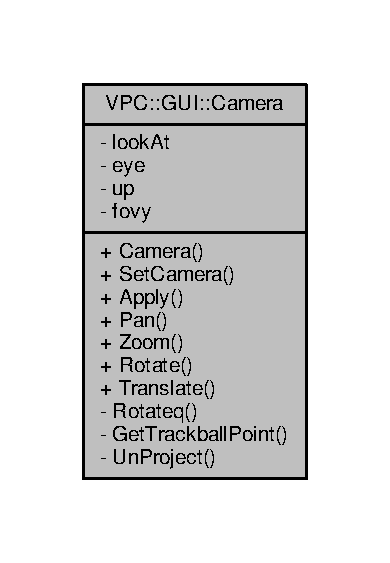
\includegraphics[width=187pt]{class_v_p_c_1_1_g_u_i_1_1_camera__coll__graph}
\end{center}
\end{figure}
\subsection*{Publiskās elementa funkcijas}
\begin{DoxyCompactItemize}
\item 
\hyperlink{class_v_p_c_1_1_g_u_i_1_1_camera_ae699f409e3205018175f7bd8b3eab657}{Camera} ()
\item 
void \hyperlink{class_v_p_c_1_1_g_u_i_1_1_camera_a5e28472053c4188219683939cad01f1f}{Set\+Camera} (const Eigen\+::\+Vector3d \&\hyperlink{class_v_p_c_1_1_g_u_i_1_1_camera_a41fa78ce129c9f56edc54f0cf7c8d60a}{look\+At}, const Eigen\+::\+Vector3d \&\hyperlink{class_v_p_c_1_1_g_u_i_1_1_camera_aa8d4d1fb2e40a19c1a18bcf04728e64a}{eye}, const Eigen\+::\+Vector3d \&\hyperlink{class_v_p_c_1_1_g_u_i_1_1_camera_a92bf7bde4d049ff9b23a304aa562e698}{up})
\item 
void \hyperlink{class_v_p_c_1_1_g_u_i_1_1_camera_a30bd1c97b4736674333192813ca9a8e1}{Apply} ()
\item 
void \hyperlink{class_v_p_c_1_1_g_u_i_1_1_camera_a04f129748aac202d1d3d9ea5f55af125}{Pan} (int x, int y, int prev\+\_\+x, int prev\+\_\+y)
\item 
void \hyperlink{class_v_p_c_1_1_g_u_i_1_1_camera_abdde0bfa7ddf8fbd1e7f04f8865797cd}{Zoom} (int x, int y, int prev\+\_\+x, int prev\+\_\+y)
\item 
void \hyperlink{class_v_p_c_1_1_g_u_i_1_1_camera_a9f41d355bea421e7403de20db33ed069}{Rotate} (int x, int y, int prev\+\_\+x, int prev\+\_\+y)
\item 
void \hyperlink{class_v_p_c_1_1_g_u_i_1_1_camera_ae2bdc4748463c831a9bc2170d0b420b1}{Translate} (int x, int y, int prev\+\_\+x, int prev\+\_\+y)
\end{DoxyCompactItemize}
\subsection*{Privātās elementa funkcijas}
\begin{DoxyCompactItemize}
\item 
Eigen\+::\+Vector3d \hyperlink{class_v_p_c_1_1_g_u_i_1_1_camera_a3bca13fbbe8272562b7261037e991860}{Rotateq} (const Eigen\+::\+Vector3d \&target, const Eigen\+::\+Vector3d \&rotate\+Vector, double angle)
\item 
Eigen\+::\+Vector3d \hyperlink{class_v_p_c_1_1_g_u_i_1_1_camera_acf91e9c32fceb9143c7dd41d45ccafca}{Get\+Trackball\+Point} (int mouseX, int mouseY, int w, int h)
\item 
Eigen\+::\+Vector3d \hyperlink{class_v_p_c_1_1_g_u_i_1_1_camera_af5f9325fafe1d0015c785d077f5c5319}{Un\+Project} (const Eigen\+::\+Vector3d \&vec)
\end{DoxyCompactItemize}
\subsection*{Privātie atribūti}
\begin{DoxyCompactItemize}
\item 
Eigen\+::\+Vector3d \hyperlink{class_v_p_c_1_1_g_u_i_1_1_camera_a41fa78ce129c9f56edc54f0cf7c8d60a}{look\+At}
\item 
Eigen\+::\+Vector3d \hyperlink{class_v_p_c_1_1_g_u_i_1_1_camera_aa8d4d1fb2e40a19c1a18bcf04728e64a}{eye}
\item 
Eigen\+::\+Vector3d \hyperlink{class_v_p_c_1_1_g_u_i_1_1_camera_a92bf7bde4d049ff9b23a304aa562e698}{up}
\item 
double \hyperlink{class_v_p_c_1_1_g_u_i_1_1_camera_a34f22355b6221876ea44fbfd866471b1}{fovy}
\end{DoxyCompactItemize}


\subsection{Detalizēts apraksts}


Definēts līnijā 8 failā Camera.\+h.



\subsection{Konstruktora un destruktora dokumentācija}
\index{V\+P\+C\+::\+G\+U\+I\+::\+Camera@{V\+P\+C\+::\+G\+U\+I\+::\+Camera}!Camera@{Camera}}
\index{Camera@{Camera}!V\+P\+C\+::\+G\+U\+I\+::\+Camera@{V\+P\+C\+::\+G\+U\+I\+::\+Camera}}
\subsubsection[{\texorpdfstring{Camera()}{Camera()}}]{\setlength{\rightskip}{0pt plus 5cm}V\+P\+C\+::\+G\+U\+I\+::\+Camera\+::\+Camera (
\begin{DoxyParamCaption}
{}
\end{DoxyParamCaption}
)}\hypertarget{class_v_p_c_1_1_g_u_i_1_1_camera_ae699f409e3205018175f7bd8b3eab657}{}\label{class_v_p_c_1_1_g_u_i_1_1_camera_ae699f409e3205018175f7bd8b3eab657}


Definēts līnijā 6 failā Camera.\+cpp.


\begin{DoxyCode}
8     :\hyperlink{class_v_p_c_1_1_g_u_i_1_1_camera_a34f22355b6221876ea44fbfd866471b1}{fovy}(60.0),\hyperlink{class_v_p_c_1_1_g_u_i_1_1_camera_a41fa78ce129c9f56edc54f0cf7c8d60a}{lookAt}(Eigen::Vector3d(0,0.5,0)),\hyperlink{class_v_p_c_1_1_g_u_i_1_1_camera_aa8d4d1fb2e40a19c1a18bcf04728e64a}{eye}(Eigen::Vector3d(3.0,0.5,0.0)),
      \hyperlink{class_v_p_c_1_1_g_u_i_1_1_camera_a92bf7bde4d049ff9b23a304aa562e698}{up}(Eigen::Vector3d(0,1,0))
9 \{
10 
11 \}
\end{DoxyCode}


Šeit ir visu funkciju izsaugumu grafs\+:
\nopagebreak
\begin{figure}[H]
\begin{center}
\leavevmode
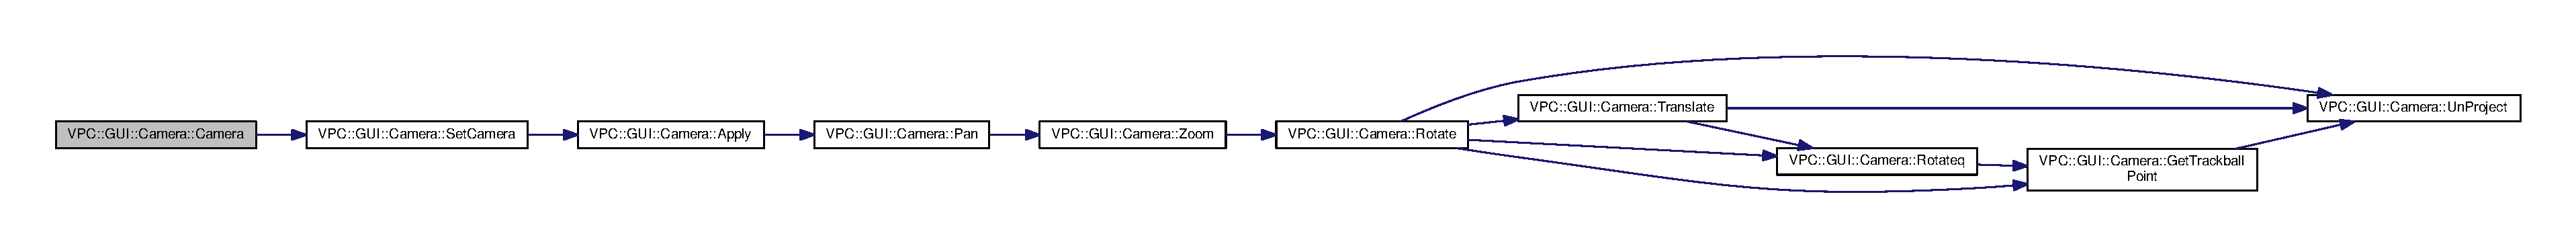
\includegraphics[width=350pt]{class_v_p_c_1_1_g_u_i_1_1_camera_ae699f409e3205018175f7bd8b3eab657_cgraph}
\end{center}
\end{figure}




\subsection{Elementa funkcijas dokumentācija}
\index{V\+P\+C\+::\+G\+U\+I\+::\+Camera@{V\+P\+C\+::\+G\+U\+I\+::\+Camera}!Apply@{Apply}}
\index{Apply@{Apply}!V\+P\+C\+::\+G\+U\+I\+::\+Camera@{V\+P\+C\+::\+G\+U\+I\+::\+Camera}}
\subsubsection[{\texorpdfstring{Apply()}{Apply()}}]{\setlength{\rightskip}{0pt plus 5cm}void V\+P\+C\+::\+G\+U\+I\+::\+Camera\+::\+Apply (
\begin{DoxyParamCaption}
{}
\end{DoxyParamCaption}
)}\hypertarget{class_v_p_c_1_1_g_u_i_1_1_camera_a30bd1c97b4736674333192813ca9a8e1}{}\label{class_v_p_c_1_1_g_u_i_1_1_camera_a30bd1c97b4736674333192813ca9a8e1}


Definēts līnijā 21 failā Camera.\+cpp.


\begin{DoxyCode}
22 \{
23     GLint w = glutGet(GLUT\_WINDOW\_WIDTH);
24     GLint h = glutGet(GLUT\_WINDOW\_HEIGHT);
25     glMatrixMode(GL\_PROJECTION);
26     glLoadIdentity();
27     gluPerspective(\hyperlink{class_v_p_c_1_1_g_u_i_1_1_camera_a34f22355b6221876ea44fbfd866471b1}{fovy}, (GLfloat)w / (GLfloat)h, 0.01, 1000);
28     glMatrixMode(GL\_MODELVIEW);
29     glLoadIdentity();
30     gluLookAt(\hyperlink{class_v_p_c_1_1_g_u_i_1_1_camera_aa8d4d1fb2e40a19c1a18bcf04728e64a}{eye}.x(), \hyperlink{class_v_p_c_1_1_g_u_i_1_1_camera_aa8d4d1fb2e40a19c1a18bcf04728e64a}{eye}.y(), \hyperlink{class_v_p_c_1_1_g_u_i_1_1_camera_aa8d4d1fb2e40a19c1a18bcf04728e64a}{eye}.z(),
31         \hyperlink{class_v_p_c_1_1_g_u_i_1_1_camera_a41fa78ce129c9f56edc54f0cf7c8d60a}{lookAt}.x(), \hyperlink{class_v_p_c_1_1_g_u_i_1_1_camera_a41fa78ce129c9f56edc54f0cf7c8d60a}{lookAt}.y(), \hyperlink{class_v_p_c_1_1_g_u_i_1_1_camera_a41fa78ce129c9f56edc54f0cf7c8d60a}{lookAt}.z(),
32         \hyperlink{class_v_p_c_1_1_g_u_i_1_1_camera_a92bf7bde4d049ff9b23a304aa562e698}{up}.x(), \hyperlink{class_v_p_c_1_1_g_u_i_1_1_camera_a92bf7bde4d049ff9b23a304aa562e698}{up}.y(), \hyperlink{class_v_p_c_1_1_g_u_i_1_1_camera_a92bf7bde4d049ff9b23a304aa562e698}{up}.z());
33 \}
\end{DoxyCode}


Šeit ir visu funkciju izsaugumu grafs\+:
\nopagebreak
\begin{figure}[H]
\begin{center}
\leavevmode
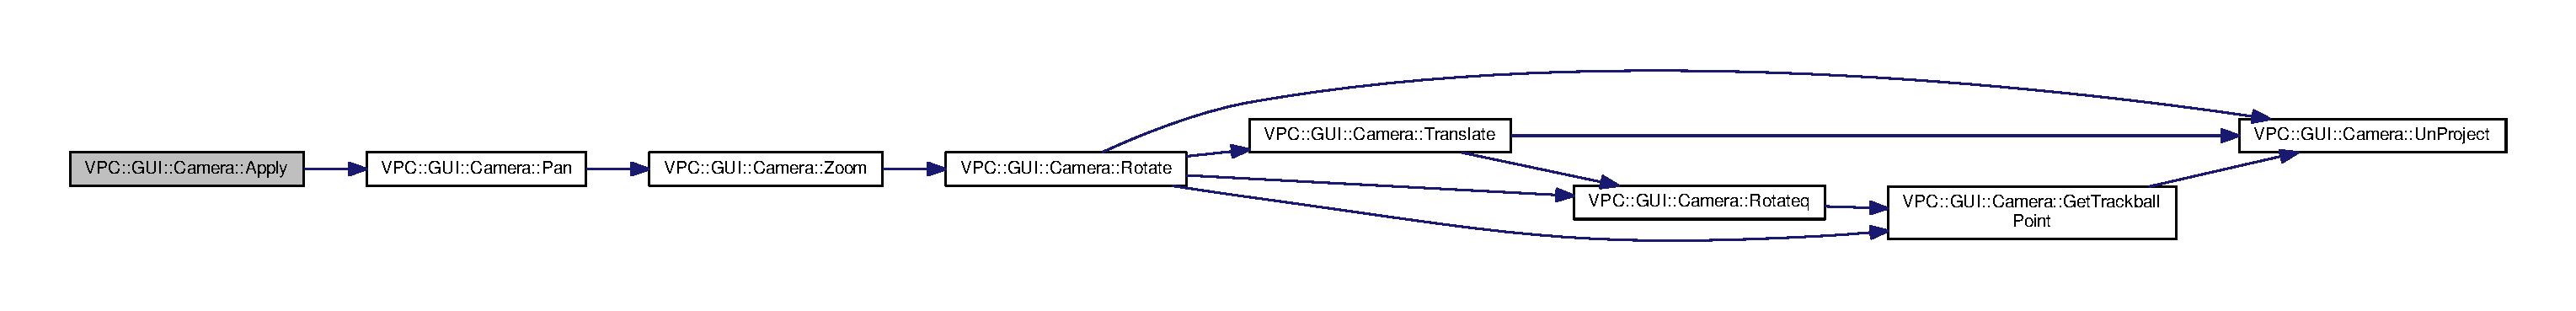
\includegraphics[width=350pt]{class_v_p_c_1_1_g_u_i_1_1_camera_a30bd1c97b4736674333192813ca9a8e1_cgraph}
\end{center}
\end{figure}




Šeit ir šīs funkcijas izsaukuma grafs\+:
\nopagebreak
\begin{figure}[H]
\begin{center}
\leavevmode
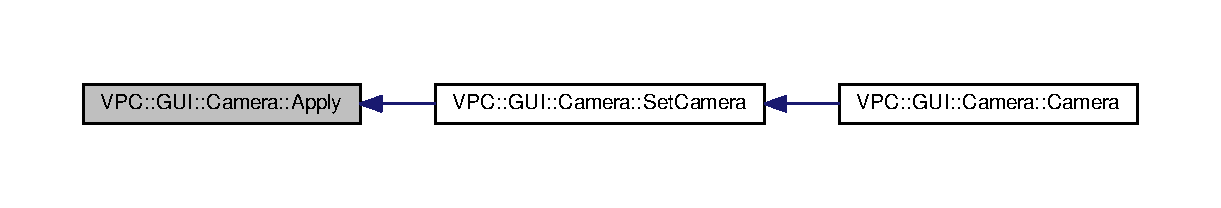
\includegraphics[width=350pt]{class_v_p_c_1_1_g_u_i_1_1_camera_a30bd1c97b4736674333192813ca9a8e1_icgraph}
\end{center}
\end{figure}


\index{V\+P\+C\+::\+G\+U\+I\+::\+Camera@{V\+P\+C\+::\+G\+U\+I\+::\+Camera}!Get\+Trackball\+Point@{Get\+Trackball\+Point}}
\index{Get\+Trackball\+Point@{Get\+Trackball\+Point}!V\+P\+C\+::\+G\+U\+I\+::\+Camera@{V\+P\+C\+::\+G\+U\+I\+::\+Camera}}
\subsubsection[{\texorpdfstring{Get\+Trackball\+Point(int mouse\+X, int mouse\+Y, int w, int h)}{GetTrackballPoint(int mouseX, int mouseY, int w, int h)}}]{\setlength{\rightskip}{0pt plus 5cm}Eigen\+::\+Vector3d V\+P\+C\+::\+G\+U\+I\+::\+Camera\+::\+Get\+Trackball\+Point (
\begin{DoxyParamCaption}
\item[{int}]{mouseX, }
\item[{int}]{mouseY, }
\item[{int}]{w, }
\item[{int}]{h}
\end{DoxyParamCaption}
)\hspace{0.3cm}{\ttfamily [private]}}\hypertarget{class_v_p_c_1_1_g_u_i_1_1_camera_acf91e9c32fceb9143c7dd41d45ccafca}{}\label{class_v_p_c_1_1_g_u_i_1_1_camera_acf91e9c32fceb9143c7dd41d45ccafca}


Definēts līnijā 98 failā Camera.\+cpp.


\begin{DoxyCode}
99 \{
100     \textcolor{keywordtype}{double} rad = sqrt((\textcolor{keywordtype}{double})(w*w+h*h)) / 2.0;
101     \textcolor{keywordtype}{double} dx = (double)(mouseX)-(double)w / 2.0;
102     \textcolor{keywordtype}{double} dy = (double)(mouseY)-(double)h / 2.0;
103     \textcolor{keywordtype}{double} dx2pdy2 = dx*dx + dy*dy;
104 
105     \textcolor{keywordflow}{if} (rad*rad - dx2pdy2 <= 0)
106         \textcolor{keywordflow}{return} Eigen::Vector3d(dx, dy, 0);
107     \textcolor{keywordflow}{else}
108         \textcolor{keywordflow}{return} Eigen::Vector3d(dx, dy, sqrt(rad*rad - dx*dx - dy*dy));
109 \}
\end{DoxyCode}


Šeit ir visu funkciju izsaugumu grafs\+:
\nopagebreak
\begin{figure}[H]
\begin{center}
\leavevmode
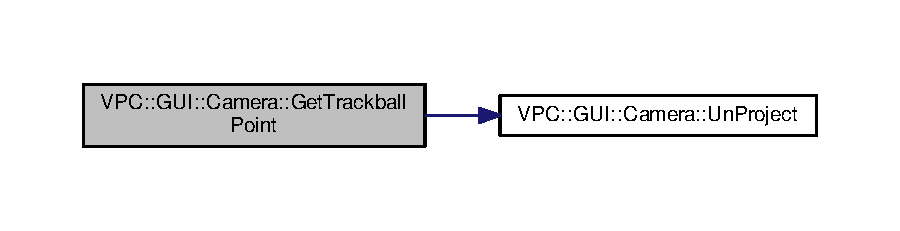
\includegraphics[width=350pt]{class_v_p_c_1_1_g_u_i_1_1_camera_acf91e9c32fceb9143c7dd41d45ccafca_cgraph}
\end{center}
\end{figure}




Šeit ir šīs funkcijas izsaukuma grafs\+:
\nopagebreak
\begin{figure}[H]
\begin{center}
\leavevmode
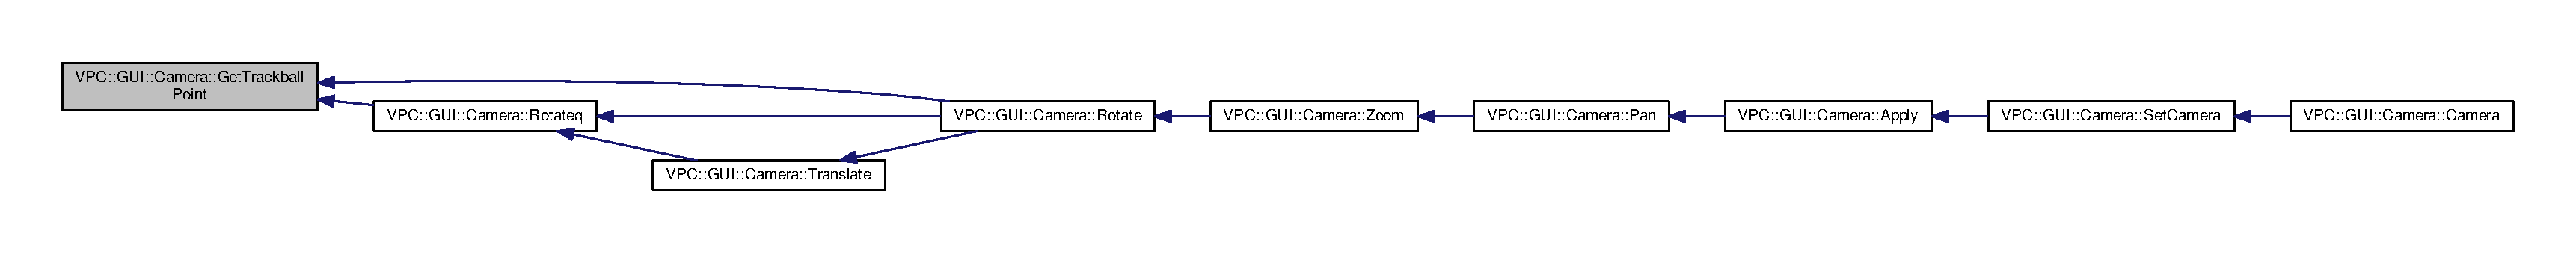
\includegraphics[width=350pt]{class_v_p_c_1_1_g_u_i_1_1_camera_acf91e9c32fceb9143c7dd41d45ccafca_icgraph}
\end{center}
\end{figure}


\index{V\+P\+C\+::\+G\+U\+I\+::\+Camera@{V\+P\+C\+::\+G\+U\+I\+::\+Camera}!Pan@{Pan}}
\index{Pan@{Pan}!V\+P\+C\+::\+G\+U\+I\+::\+Camera@{V\+P\+C\+::\+G\+U\+I\+::\+Camera}}
\subsubsection[{\texorpdfstring{Pan(int x, int y, int prev\+\_\+x, int prev\+\_\+y)}{Pan(int x, int y, int prev_x, int prev_y)}}]{\setlength{\rightskip}{0pt plus 5cm}void V\+P\+C\+::\+G\+U\+I\+::\+Camera\+::\+Pan (
\begin{DoxyParamCaption}
\item[{int}]{x, }
\item[{int}]{y, }
\item[{int}]{prev\+\_\+x, }
\item[{int}]{prev\+\_\+y}
\end{DoxyParamCaption}
)}\hypertarget{class_v_p_c_1_1_g_u_i_1_1_camera_a04f129748aac202d1d3d9ea5f55af125}{}\label{class_v_p_c_1_1_g_u_i_1_1_camera_a04f129748aac202d1d3d9ea5f55af125}


Definēts līnijā 37 failā Camera.\+cpp.


\begin{DoxyCode}
38 \{
39     \textcolor{keywordtype}{double} delta = (double)prev\_y - (\textcolor{keywordtype}{double})y;
40     delta = 1 - delta / 200.0;
41     \hyperlink{class_v_p_c_1_1_g_u_i_1_1_camera_aa8d4d1fb2e40a19c1a18bcf04728e64a}{eye} = \hyperlink{class_v_p_c_1_1_g_u_i_1_1_camera_a41fa78ce129c9f56edc54f0cf7c8d60a}{lookAt} - (\hyperlink{class_v_p_c_1_1_g_u_i_1_1_camera_a41fa78ce129c9f56edc54f0cf7c8d60a}{lookAt} - \hyperlink{class_v_p_c_1_1_g_u_i_1_1_camera_aa8d4d1fb2e40a19c1a18bcf04728e64a}{eye})*delta;
42 \}
\end{DoxyCode}


Šeit ir visu funkciju izsaugumu grafs\+:
\nopagebreak
\begin{figure}[H]
\begin{center}
\leavevmode
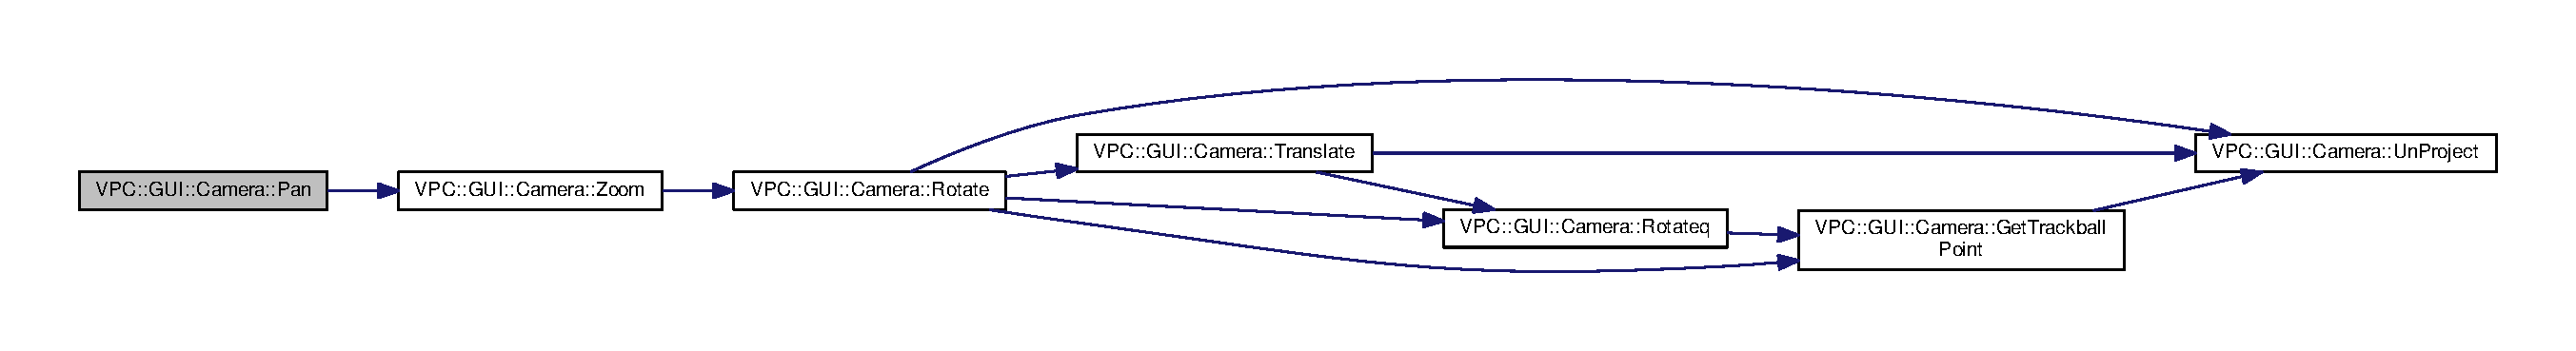
\includegraphics[width=350pt]{class_v_p_c_1_1_g_u_i_1_1_camera_a04f129748aac202d1d3d9ea5f55af125_cgraph}
\end{center}
\end{figure}




Šeit ir šīs funkcijas izsaukuma grafs\+:
\nopagebreak
\begin{figure}[H]
\begin{center}
\leavevmode
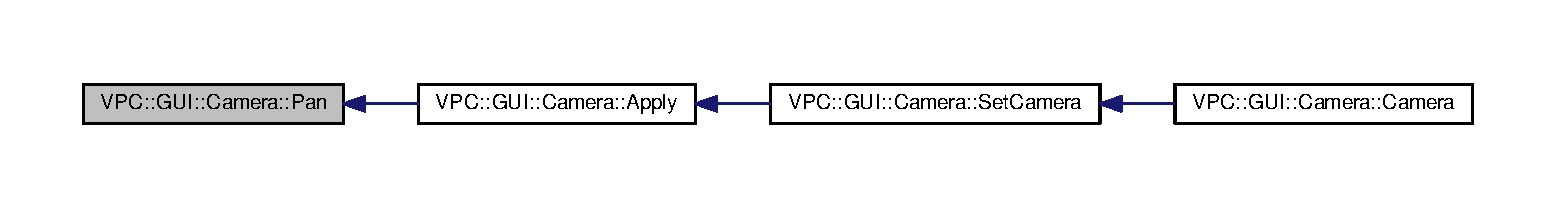
\includegraphics[width=350pt]{class_v_p_c_1_1_g_u_i_1_1_camera_a04f129748aac202d1d3d9ea5f55af125_icgraph}
\end{center}
\end{figure}


\index{V\+P\+C\+::\+G\+U\+I\+::\+Camera@{V\+P\+C\+::\+G\+U\+I\+::\+Camera}!Rotate@{Rotate}}
\index{Rotate@{Rotate}!V\+P\+C\+::\+G\+U\+I\+::\+Camera@{V\+P\+C\+::\+G\+U\+I\+::\+Camera}}
\subsubsection[{\texorpdfstring{Rotate(int x, int y, int prev\+\_\+x, int prev\+\_\+y)}{Rotate(int x, int y, int prev_x, int prev_y)}}]{\setlength{\rightskip}{0pt plus 5cm}void V\+P\+C\+::\+G\+U\+I\+::\+Camera\+::\+Rotate (
\begin{DoxyParamCaption}
\item[{int}]{x, }
\item[{int}]{y, }
\item[{int}]{prev\+\_\+x, }
\item[{int}]{prev\+\_\+y}
\end{DoxyParamCaption}
)}\hypertarget{class_v_p_c_1_1_g_u_i_1_1_camera_a9f41d355bea421e7403de20db33ed069}{}\label{class_v_p_c_1_1_g_u_i_1_1_camera_a9f41d355bea421e7403de20db33ed069}


Definēts līnijā 52 failā Camera.\+cpp.


\begin{DoxyCode}
53 \{
54     GLint w = glutGet(GLUT\_WINDOW\_WIDTH);
55     GLint h = glutGet(GLUT\_WINDOW\_HEIGHT);
56 
57     Eigen::Vector3d prevPoint = \hyperlink{class_v_p_c_1_1_g_u_i_1_1_camera_acf91e9c32fceb9143c7dd41d45ccafca}{GetTrackballPoint}(prev\_x,prev\_y,w,h);
58     Eigen::Vector3d curPoint = \hyperlink{class_v_p_c_1_1_g_u_i_1_1_camera_acf91e9c32fceb9143c7dd41d45ccafca}{GetTrackballPoint}(x,y,w,h);
59     Eigen::Vector3d rotVec = curPoint.cross(prevPoint);
60 
61     rotVec = \hyperlink{class_v_p_c_1_1_g_u_i_1_1_camera_af5f9325fafe1d0015c785d077f5c5319}{UnProject}(rotVec);
62     \textcolor{keywordtype}{double} cosT = curPoint.dot(prevPoint) / (curPoint.norm()*prevPoint.norm());
63     \textcolor{keywordtype}{double} sinT = (curPoint.cross(prevPoint)).norm() / (curPoint.norm()*prevPoint.norm());
64 
65     \textcolor{keywordtype}{double} angle = -atan2(sinT, cosT);
66 
67     Eigen::Vector3d n = this->\hyperlink{class_v_p_c_1_1_g_u_i_1_1_camera_a41fa78ce129c9f56edc54f0cf7c8d60a}{lookAt} - this->\hyperlink{class_v_p_c_1_1_g_u_i_1_1_camera_aa8d4d1fb2e40a19c1a18bcf04728e64a}{eye};
68     n = \hyperlink{class_v_p_c_1_1_g_u_i_1_1_camera_a3bca13fbbe8272562b7261037e991860}{Rotateq}(n, rotVec, angle);
69     this->\hyperlink{class_v_p_c_1_1_g_u_i_1_1_camera_a92bf7bde4d049ff9b23a304aa562e698}{up} = \hyperlink{class_v_p_c_1_1_g_u_i_1_1_camera_a3bca13fbbe8272562b7261037e991860}{Rotateq}(this->\hyperlink{class_v_p_c_1_1_g_u_i_1_1_camera_a92bf7bde4d049ff9b23a304aa562e698}{up}, rotVec, angle);
70     this->eye = this->\hyperlink{class_v_p_c_1_1_g_u_i_1_1_camera_a41fa78ce129c9f56edc54f0cf7c8d60a}{lookAt} - n;
71 \}
\end{DoxyCode}


Šeit ir visu funkciju izsaugumu grafs\+:
\nopagebreak
\begin{figure}[H]
\begin{center}
\leavevmode
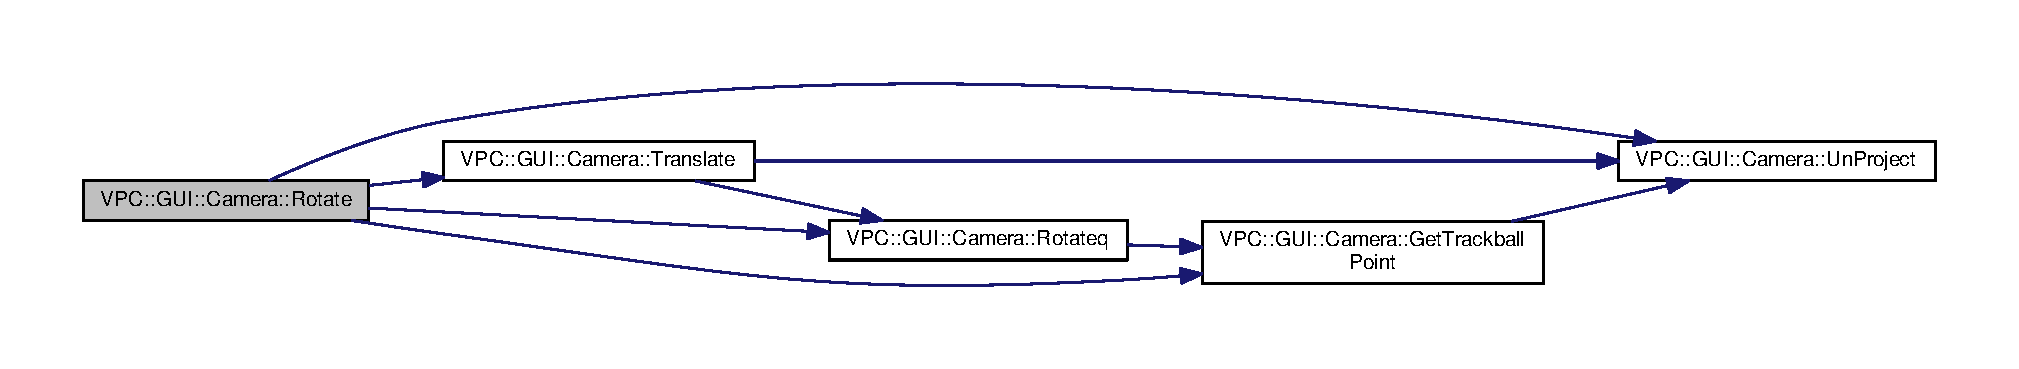
\includegraphics[width=350pt]{class_v_p_c_1_1_g_u_i_1_1_camera_a9f41d355bea421e7403de20db33ed069_cgraph}
\end{center}
\end{figure}




Šeit ir šīs funkcijas izsaukuma grafs\+:
\nopagebreak
\begin{figure}[H]
\begin{center}
\leavevmode
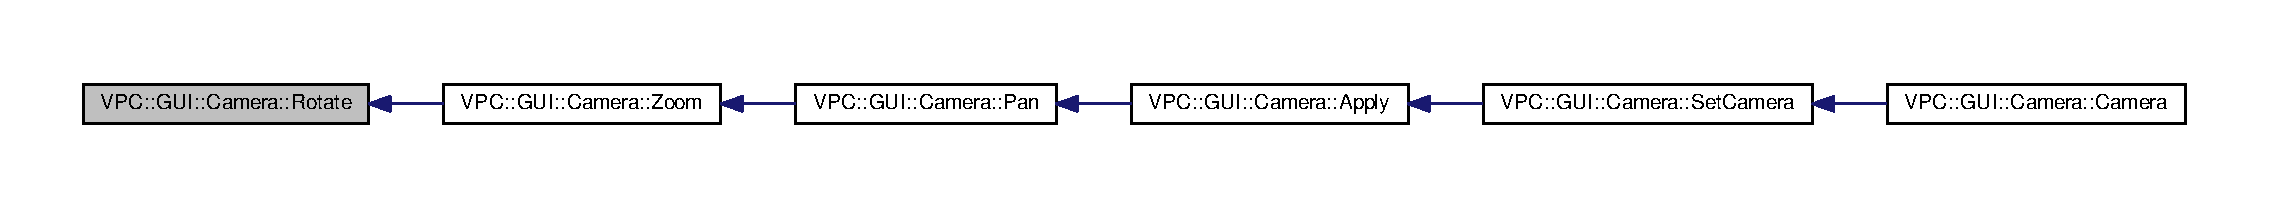
\includegraphics[width=350pt]{class_v_p_c_1_1_g_u_i_1_1_camera_a9f41d355bea421e7403de20db33ed069_icgraph}
\end{center}
\end{figure}


\index{V\+P\+C\+::\+G\+U\+I\+::\+Camera@{V\+P\+C\+::\+G\+U\+I\+::\+Camera}!Rotateq@{Rotateq}}
\index{Rotateq@{Rotateq}!V\+P\+C\+::\+G\+U\+I\+::\+Camera@{V\+P\+C\+::\+G\+U\+I\+::\+Camera}}
\subsubsection[{\texorpdfstring{Rotateq(const Eigen\+::\+Vector3d \&target, const Eigen\+::\+Vector3d \&rotate\+Vector, double angle)}{Rotateq(const Eigen::Vector3d &target, const Eigen::Vector3d &rotateVector, double angle)}}]{\setlength{\rightskip}{0pt plus 5cm}Eigen\+::\+Vector3d V\+P\+C\+::\+G\+U\+I\+::\+Camera\+::\+Rotateq (
\begin{DoxyParamCaption}
\item[{const Eigen\+::\+Vector3d \&}]{target, }
\item[{const Eigen\+::\+Vector3d \&}]{rotate\+Vector, }
\item[{double}]{angle}
\end{DoxyParamCaption}
)\hspace{0.3cm}{\ttfamily [private]}}\hypertarget{class_v_p_c_1_1_g_u_i_1_1_camera_a3bca13fbbe8272562b7261037e991860}{}\label{class_v_p_c_1_1_g_u_i_1_1_camera_a3bca13fbbe8272562b7261037e991860}


Definēts līnijā 83 failā Camera.\+cpp.


\begin{DoxyCode}
84 \{
85     Eigen::Vector3d rv = rotateVector.normalized();
86 
87     Eigen::Quaternion<double> rot(cos(angle / 2.0), sin(angle / 2.0)*rv.x(), sin(angle / 2.0)*rv.y(), sin(
      angle / 2.0)*rv.z());
88     rot.normalize();
89     Eigen::Quaternion<double> tar(0, target.x(), target.y(), target.z());
90 
91 
92     tar = rot.inverse()*tar*rot;
93 
94     \textcolor{keywordflow}{return} Eigen::Vector3d(tar.x(), tar.y(), tar.z());
95 \}
\end{DoxyCode}


Šeit ir visu funkciju izsaugumu grafs\+:
\nopagebreak
\begin{figure}[H]
\begin{center}
\leavevmode
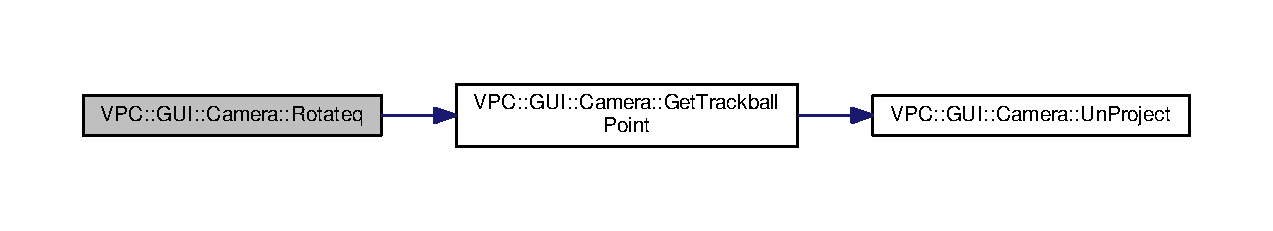
\includegraphics[width=350pt]{class_v_p_c_1_1_g_u_i_1_1_camera_a3bca13fbbe8272562b7261037e991860_cgraph}
\end{center}
\end{figure}




Šeit ir šīs funkcijas izsaukuma grafs\+:
\nopagebreak
\begin{figure}[H]
\begin{center}
\leavevmode
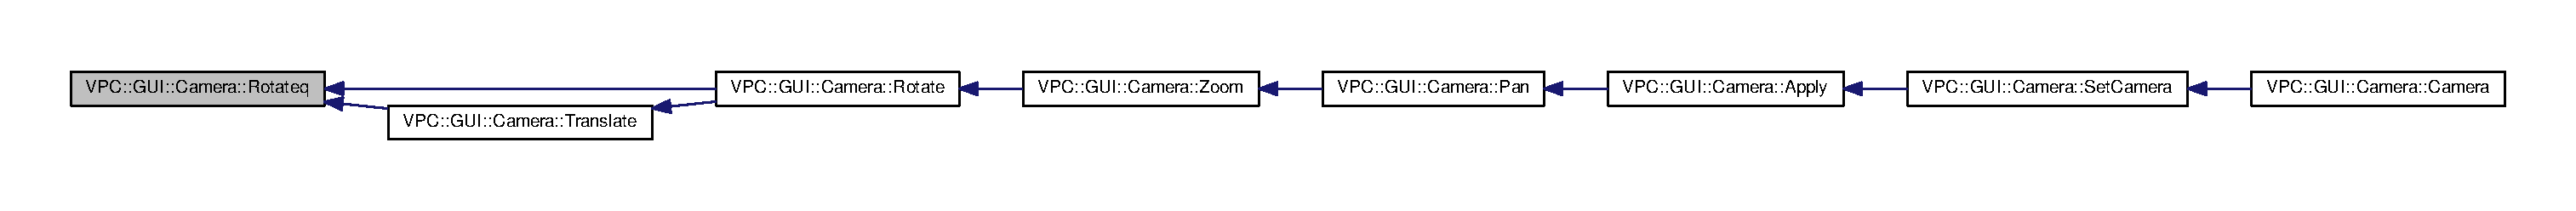
\includegraphics[width=350pt]{class_v_p_c_1_1_g_u_i_1_1_camera_a3bca13fbbe8272562b7261037e991860_icgraph}
\end{center}
\end{figure}


\index{V\+P\+C\+::\+G\+U\+I\+::\+Camera@{V\+P\+C\+::\+G\+U\+I\+::\+Camera}!Set\+Camera@{Set\+Camera}}
\index{Set\+Camera@{Set\+Camera}!V\+P\+C\+::\+G\+U\+I\+::\+Camera@{V\+P\+C\+::\+G\+U\+I\+::\+Camera}}
\subsubsection[{\texorpdfstring{Set\+Camera(const Eigen\+::\+Vector3d \&look\+At, const Eigen\+::\+Vector3d \&eye, const Eigen\+::\+Vector3d \&up)}{SetCamera(const Eigen::Vector3d &lookAt, const Eigen::Vector3d &eye, const Eigen::Vector3d &up)}}]{\setlength{\rightskip}{0pt plus 5cm}void V\+P\+C\+::\+G\+U\+I\+::\+Camera\+::\+Set\+Camera (
\begin{DoxyParamCaption}
\item[{const Eigen\+::\+Vector3d \&}]{look\+At, }
\item[{const Eigen\+::\+Vector3d \&}]{eye, }
\item[{const Eigen\+::\+Vector3d \&}]{up}
\end{DoxyParamCaption}
)}\hypertarget{class_v_p_c_1_1_g_u_i_1_1_camera_a5e28472053c4188219683939cad01f1f}{}\label{class_v_p_c_1_1_g_u_i_1_1_camera_a5e28472053c4188219683939cad01f1f}


Definēts līnijā 15 failā Camera.\+cpp.


\begin{DoxyCode}
16 \{
17     this->\hyperlink{class_v_p_c_1_1_g_u_i_1_1_camera_a41fa78ce129c9f56edc54f0cf7c8d60a}{lookAt} = \hyperlink{class_v_p_c_1_1_g_u_i_1_1_camera_a41fa78ce129c9f56edc54f0cf7c8d60a}{lookAt}, this->\hyperlink{class_v_p_c_1_1_g_u_i_1_1_camera_aa8d4d1fb2e40a19c1a18bcf04728e64a}{eye} = \hyperlink{class_v_p_c_1_1_g_u_i_1_1_camera_aa8d4d1fb2e40a19c1a18bcf04728e64a}{eye}, this->\hyperlink{class_v_p_c_1_1_g_u_i_1_1_camera_a92bf7bde4d049ff9b23a304aa562e698}{up} = \hyperlink{class_v_p_c_1_1_g_u_i_1_1_camera_a92bf7bde4d049ff9b23a304aa562e698}{up};
18 \}
\end{DoxyCode}


Šeit ir visu funkciju izsaugumu grafs\+:
\nopagebreak
\begin{figure}[H]
\begin{center}
\leavevmode
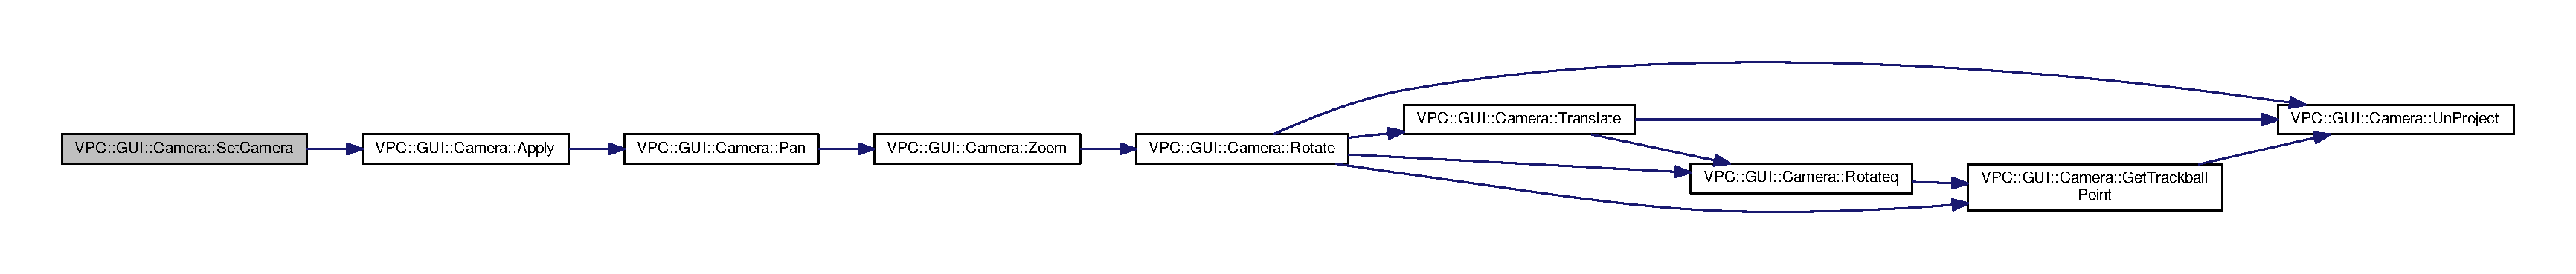
\includegraphics[width=350pt]{class_v_p_c_1_1_g_u_i_1_1_camera_a5e28472053c4188219683939cad01f1f_cgraph}
\end{center}
\end{figure}




Šeit ir šīs funkcijas izsaukuma grafs\+:
\nopagebreak
\begin{figure}[H]
\begin{center}
\leavevmode
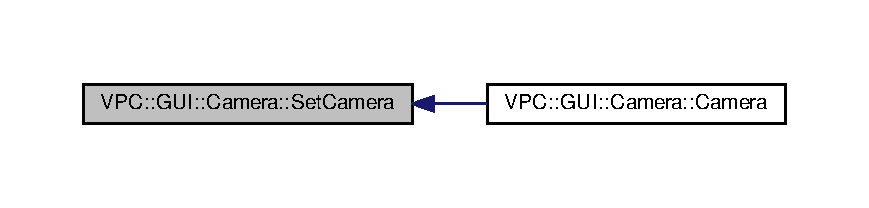
\includegraphics[width=350pt]{class_v_p_c_1_1_g_u_i_1_1_camera_a5e28472053c4188219683939cad01f1f_icgraph}
\end{center}
\end{figure}


\index{V\+P\+C\+::\+G\+U\+I\+::\+Camera@{V\+P\+C\+::\+G\+U\+I\+::\+Camera}!Translate@{Translate}}
\index{Translate@{Translate}!V\+P\+C\+::\+G\+U\+I\+::\+Camera@{V\+P\+C\+::\+G\+U\+I\+::\+Camera}}
\subsubsection[{\texorpdfstring{Translate(int x, int y, int prev\+\_\+x, int prev\+\_\+y)}{Translate(int x, int y, int prev_x, int prev_y)}}]{\setlength{\rightskip}{0pt plus 5cm}void V\+P\+C\+::\+G\+U\+I\+::\+Camera\+::\+Translate (
\begin{DoxyParamCaption}
\item[{int}]{x, }
\item[{int}]{y, }
\item[{int}]{prev\+\_\+x, }
\item[{int}]{prev\+\_\+y}
\end{DoxyParamCaption}
)}\hypertarget{class_v_p_c_1_1_g_u_i_1_1_camera_ae2bdc4748463c831a9bc2170d0b420b1}{}\label{class_v_p_c_1_1_g_u_i_1_1_camera_ae2bdc4748463c831a9bc2170d0b420b1}


Definēts līnijā 74 failā Camera.\+cpp.


\begin{DoxyCode}
75 \{
76     Eigen::Vector3d delta((\textcolor{keywordtype}{double})x - (\textcolor{keywordtype}{double})prev\_x, (\textcolor{keywordtype}{double})y - (\textcolor{keywordtype}{double})prev\_y, 0);
77     delta = \hyperlink{class_v_p_c_1_1_g_u_i_1_1_camera_af5f9325fafe1d0015c785d077f5c5319}{UnProject}(delta) / 200.0;
78     \hyperlink{class_v_p_c_1_1_g_u_i_1_1_camera_a41fa78ce129c9f56edc54f0cf7c8d60a}{lookAt} += delta; \hyperlink{class_v_p_c_1_1_g_u_i_1_1_camera_aa8d4d1fb2e40a19c1a18bcf04728e64a}{eye} += delta;
79 \}
\end{DoxyCode}


Šeit ir visu funkciju izsaugumu grafs\+:
\nopagebreak
\begin{figure}[H]
\begin{center}
\leavevmode
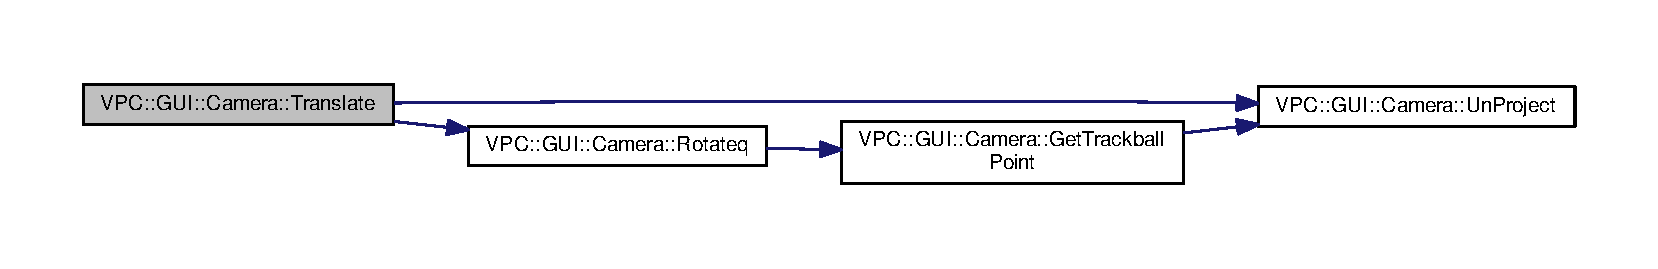
\includegraphics[width=350pt]{class_v_p_c_1_1_g_u_i_1_1_camera_ae2bdc4748463c831a9bc2170d0b420b1_cgraph}
\end{center}
\end{figure}




Šeit ir šīs funkcijas izsaukuma grafs\+:
\nopagebreak
\begin{figure}[H]
\begin{center}
\leavevmode
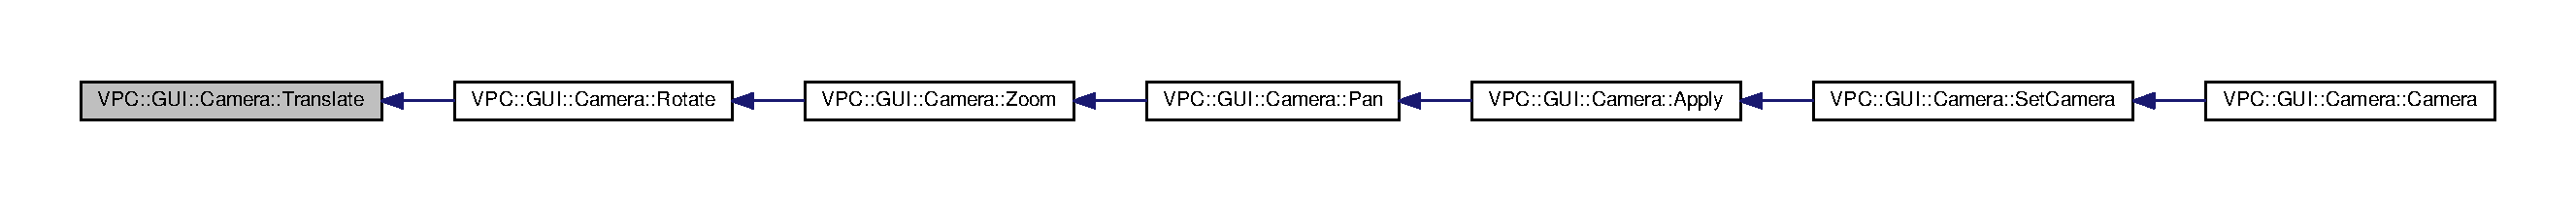
\includegraphics[width=350pt]{class_v_p_c_1_1_g_u_i_1_1_camera_ae2bdc4748463c831a9bc2170d0b420b1_icgraph}
\end{center}
\end{figure}


\index{V\+P\+C\+::\+G\+U\+I\+::\+Camera@{V\+P\+C\+::\+G\+U\+I\+::\+Camera}!Un\+Project@{Un\+Project}}
\index{Un\+Project@{Un\+Project}!V\+P\+C\+::\+G\+U\+I\+::\+Camera@{V\+P\+C\+::\+G\+U\+I\+::\+Camera}}
\subsubsection[{\texorpdfstring{Un\+Project(const Eigen\+::\+Vector3d \&vec)}{UnProject(const Eigen::Vector3d &vec)}}]{\setlength{\rightskip}{0pt plus 5cm}Eigen\+::\+Vector3d V\+P\+C\+::\+G\+U\+I\+::\+Camera\+::\+Un\+Project (
\begin{DoxyParamCaption}
\item[{const Eigen\+::\+Vector3d \&}]{vec}
\end{DoxyParamCaption}
)\hspace{0.3cm}{\ttfamily [private]}}\hypertarget{class_v_p_c_1_1_g_u_i_1_1_camera_af5f9325fafe1d0015c785d077f5c5319}{}\label{class_v_p_c_1_1_g_u_i_1_1_camera_af5f9325fafe1d0015c785d077f5c5319}


Definēts līnijā 112 failā Camera.\+cpp.


\begin{DoxyCode}
113 \{
114     Eigen::Vector3d n = \hyperlink{class_v_p_c_1_1_g_u_i_1_1_camera_a41fa78ce129c9f56edc54f0cf7c8d60a}{lookAt} - \hyperlink{class_v_p_c_1_1_g_u_i_1_1_camera_aa8d4d1fb2e40a19c1a18bcf04728e64a}{eye};
115     n.normalize();
116     
117     Eigen::Vector3d v = \hyperlink{class_v_p_c_1_1_g_u_i_1_1_camera_a92bf7bde4d049ff9b23a304aa562e698}{up}.cross(n);
118     v.normalize();
119 
120     Eigen::Vector3d u = n.cross(v);
121     u.normalize();
122 
123     \textcolor{keywordflow}{return} vec.z()*n + vec.x()*v + vec.y()*u;
124 \}
\end{DoxyCode}


Šeit ir šīs funkcijas izsaukuma grafs\+:
\nopagebreak
\begin{figure}[H]
\begin{center}
\leavevmode
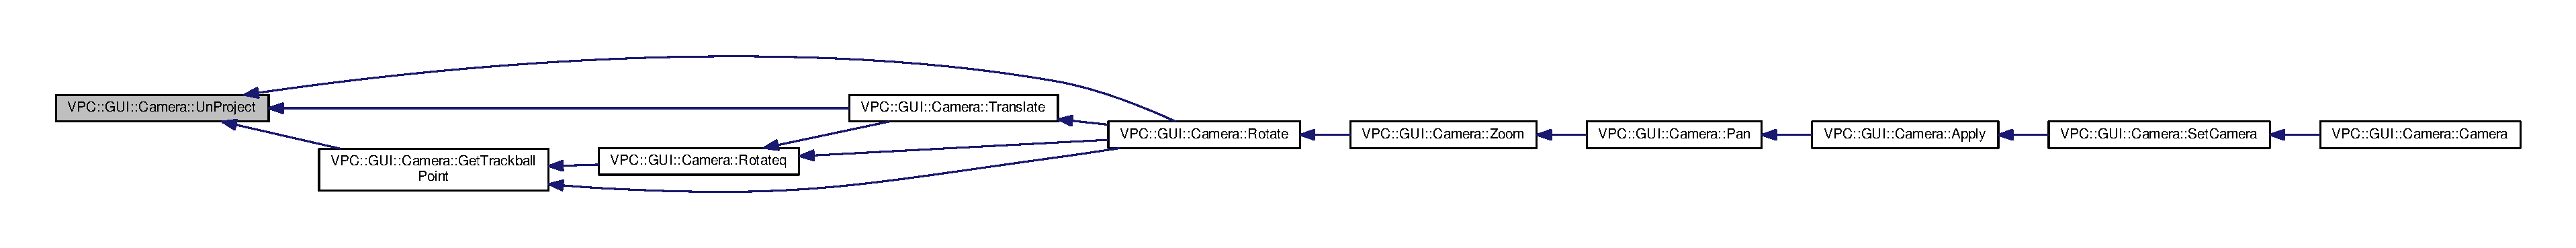
\includegraphics[width=350pt]{class_v_p_c_1_1_g_u_i_1_1_camera_af5f9325fafe1d0015c785d077f5c5319_icgraph}
\end{center}
\end{figure}


\index{V\+P\+C\+::\+G\+U\+I\+::\+Camera@{V\+P\+C\+::\+G\+U\+I\+::\+Camera}!Zoom@{Zoom}}
\index{Zoom@{Zoom}!V\+P\+C\+::\+G\+U\+I\+::\+Camera@{V\+P\+C\+::\+G\+U\+I\+::\+Camera}}
\subsubsection[{\texorpdfstring{Zoom(int x, int y, int prev\+\_\+x, int prev\+\_\+y)}{Zoom(int x, int y, int prev_x, int prev_y)}}]{\setlength{\rightskip}{0pt plus 5cm}void V\+P\+C\+::\+G\+U\+I\+::\+Camera\+::\+Zoom (
\begin{DoxyParamCaption}
\item[{int}]{x, }
\item[{int}]{y, }
\item[{int}]{prev\+\_\+x, }
\item[{int}]{prev\+\_\+y}
\end{DoxyParamCaption}
)}\hypertarget{class_v_p_c_1_1_g_u_i_1_1_camera_abdde0bfa7ddf8fbd1e7f04f8865797cd}{}\label{class_v_p_c_1_1_g_u_i_1_1_camera_abdde0bfa7ddf8fbd1e7f04f8865797cd}


Definēts līnijā 45 failā Camera.\+cpp.


\begin{DoxyCode}
46 \{
47     \textcolor{keywordtype}{double} delta = (double)prev\_y - (\textcolor{keywordtype}{double})y;
48     \hyperlink{class_v_p_c_1_1_g_u_i_1_1_camera_a34f22355b6221876ea44fbfd866471b1}{fovy} += delta/20.0;
49 \}
\end{DoxyCode}


Šeit ir visu funkciju izsaugumu grafs\+:
\nopagebreak
\begin{figure}[H]
\begin{center}
\leavevmode
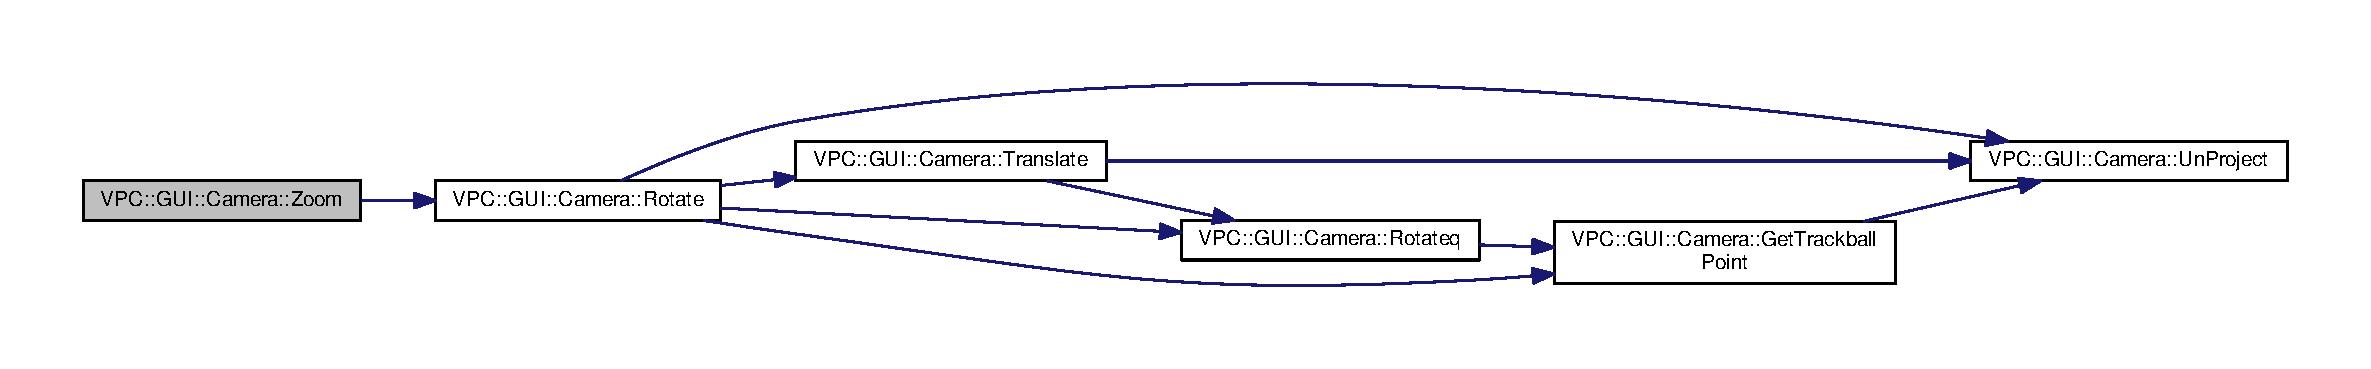
\includegraphics[width=350pt]{class_v_p_c_1_1_g_u_i_1_1_camera_abdde0bfa7ddf8fbd1e7f04f8865797cd_cgraph}
\end{center}
\end{figure}




Šeit ir šīs funkcijas izsaukuma grafs\+:
\nopagebreak
\begin{figure}[H]
\begin{center}
\leavevmode
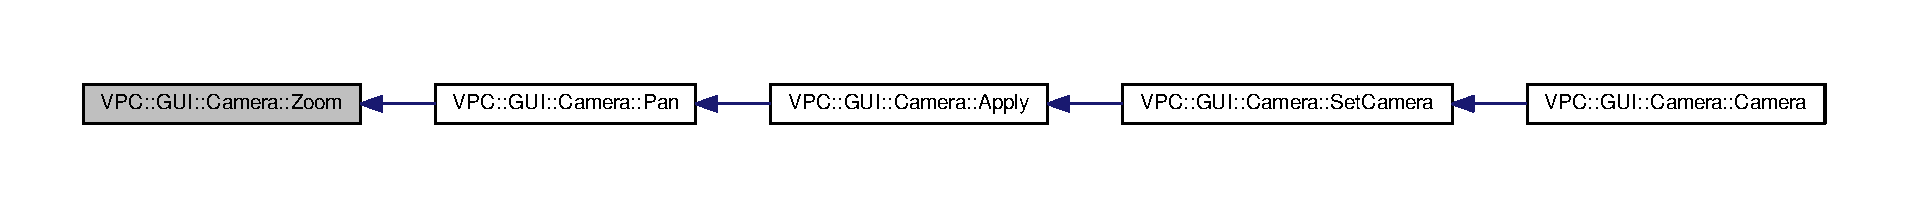
\includegraphics[width=350pt]{class_v_p_c_1_1_g_u_i_1_1_camera_abdde0bfa7ddf8fbd1e7f04f8865797cd_icgraph}
\end{center}
\end{figure}




\subsection{Elementa datu dokumentācija}
\index{V\+P\+C\+::\+G\+U\+I\+::\+Camera@{V\+P\+C\+::\+G\+U\+I\+::\+Camera}!eye@{eye}}
\index{eye@{eye}!V\+P\+C\+::\+G\+U\+I\+::\+Camera@{V\+P\+C\+::\+G\+U\+I\+::\+Camera}}
\subsubsection[{\texorpdfstring{eye}{eye}}]{\setlength{\rightskip}{0pt plus 5cm}Eigen\+::\+Vector3d V\+P\+C\+::\+G\+U\+I\+::\+Camera\+::eye\hspace{0.3cm}{\ttfamily [private]}}\hypertarget{class_v_p_c_1_1_g_u_i_1_1_camera_aa8d4d1fb2e40a19c1a18bcf04728e64a}{}\label{class_v_p_c_1_1_g_u_i_1_1_camera_aa8d4d1fb2e40a19c1a18bcf04728e64a}


Definēts līnijā 23 failā Camera.\+h.

\index{V\+P\+C\+::\+G\+U\+I\+::\+Camera@{V\+P\+C\+::\+G\+U\+I\+::\+Camera}!fovy@{fovy}}
\index{fovy@{fovy}!V\+P\+C\+::\+G\+U\+I\+::\+Camera@{V\+P\+C\+::\+G\+U\+I\+::\+Camera}}
\subsubsection[{\texorpdfstring{fovy}{fovy}}]{\setlength{\rightskip}{0pt plus 5cm}double V\+P\+C\+::\+G\+U\+I\+::\+Camera\+::fovy\hspace{0.3cm}{\ttfamily [private]}}\hypertarget{class_v_p_c_1_1_g_u_i_1_1_camera_a34f22355b6221876ea44fbfd866471b1}{}\label{class_v_p_c_1_1_g_u_i_1_1_camera_a34f22355b6221876ea44fbfd866471b1}


Definēts līnijā 25 failā Camera.\+h.

\index{V\+P\+C\+::\+G\+U\+I\+::\+Camera@{V\+P\+C\+::\+G\+U\+I\+::\+Camera}!look\+At@{look\+At}}
\index{look\+At@{look\+At}!V\+P\+C\+::\+G\+U\+I\+::\+Camera@{V\+P\+C\+::\+G\+U\+I\+::\+Camera}}
\subsubsection[{\texorpdfstring{look\+At}{lookAt}}]{\setlength{\rightskip}{0pt plus 5cm}Eigen\+::\+Vector3d V\+P\+C\+::\+G\+U\+I\+::\+Camera\+::look\+At\hspace{0.3cm}{\ttfamily [private]}}\hypertarget{class_v_p_c_1_1_g_u_i_1_1_camera_a41fa78ce129c9f56edc54f0cf7c8d60a}{}\label{class_v_p_c_1_1_g_u_i_1_1_camera_a41fa78ce129c9f56edc54f0cf7c8d60a}


Definēts līnijā 22 failā Camera.\+h.

\index{V\+P\+C\+::\+G\+U\+I\+::\+Camera@{V\+P\+C\+::\+G\+U\+I\+::\+Camera}!up@{up}}
\index{up@{up}!V\+P\+C\+::\+G\+U\+I\+::\+Camera@{V\+P\+C\+::\+G\+U\+I\+::\+Camera}}
\subsubsection[{\texorpdfstring{up}{up}}]{\setlength{\rightskip}{0pt plus 5cm}Eigen\+::\+Vector3d V\+P\+C\+::\+G\+U\+I\+::\+Camera\+::up\hspace{0.3cm}{\ttfamily [private]}}\hypertarget{class_v_p_c_1_1_g_u_i_1_1_camera_a92bf7bde4d049ff9b23a304aa562e698}{}\label{class_v_p_c_1_1_g_u_i_1_1_camera_a92bf7bde4d049ff9b23a304aa562e698}


Definēts līnijā 24 failā Camera.\+h.



Šīs klases dokumentācijas tika ģenerēta no šāda failiem\+:\begin{DoxyCompactItemize}
\item 
render/\hyperlink{_camera_8h}{Camera.\+h}\item 
render/\hyperlink{_camera_8cpp}{Camera.\+cpp}\end{DoxyCompactItemize}

\hypertarget{class_v_p_c_1_1_character}{}\section{V\+PC\+:\+:Character klases apraksts}
\label{class_v_p_c_1_1_character}\index{V\+P\+C\+::\+Character@{V\+P\+C\+::\+Character}}


{\ttfamily \#include $<$Character.\+h$>$}



Sadarbības diagramma klasei V\+PC\+:\+:Character\+:
\nopagebreak
\begin{figure}[H]
\begin{center}
\leavevmode
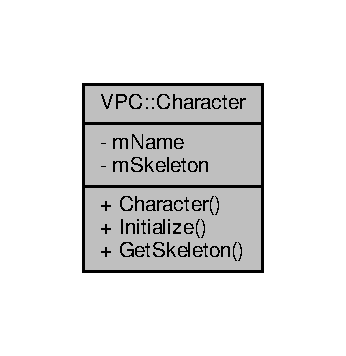
\includegraphics[width=166pt]{class_v_p_c_1_1_character__coll__graph}
\end{center}
\end{figure}
\subsection*{Publiskās elementa funkcijas}
\begin{DoxyCompactItemize}
\item 
\hyperlink{class_v_p_c_1_1_character_ab07d09bda7da4df08877ba8a82aed689}{Character} (const std\+::string name)
\item 
void \hyperlink{class_v_p_c_1_1_character_a9fb1410736359fab3877e3afe18f2877}{Initialize} ()
\item 
const dart\+::dynamics\+::\+Skeleton\+Ptr \& \hyperlink{class_v_p_c_1_1_character_ab2694f013d033805504228cb151a368f}{Get\+Skeleton} ()
\end{DoxyCompactItemize}
\subsection*{Privātie atribūti}
\begin{DoxyCompactItemize}
\item 
std\+::string \hyperlink{class_v_p_c_1_1_character_a66b5e53cb1779993ae7b78e1b29209b5}{m\+Name}
\item 
dart\+::dynamics\+::\+Skeleton\+Ptr \hyperlink{class_v_p_c_1_1_character_afbd0d7d0c6227cabd47de1a5c2d7c039}{m\+Skeleton}
\end{DoxyCompactItemize}


\subsection{Detalizēts apraksts}


Definēts līnijā 7 failā Character.\+h.



\subsection{Konstruktora un destruktora dokumentācija}
\index{V\+P\+C\+::\+Character@{V\+P\+C\+::\+Character}!Character@{Character}}
\index{Character@{Character}!V\+P\+C\+::\+Character@{V\+P\+C\+::\+Character}}
\subsubsection[{\texorpdfstring{Character(const std\+::string name)}{Character(const std::string name)}}]{\setlength{\rightskip}{0pt plus 5cm}V\+P\+C\+::\+Character\+::\+Character (
\begin{DoxyParamCaption}
\item[{const std\+::string}]{name}
\end{DoxyParamCaption}
)}\hypertarget{class_v_p_c_1_1_character_ab07d09bda7da4df08877ba8a82aed689}{}\label{class_v_p_c_1_1_character_ab07d09bda7da4df08877ba8a82aed689}


Definēts līnijā 8 failā Character.\+cpp.


\begin{DoxyCode}
9     :\hyperlink{class_v_p_c_1_1_character_a66b5e53cb1779993ae7b78e1b29209b5}{mName}(name)
10 \{
11     
12 \}
\end{DoxyCode}


Šeit ir visu funkciju izsaugumu grafs\+:
\nopagebreak
\begin{figure}[H]
\begin{center}
\leavevmode
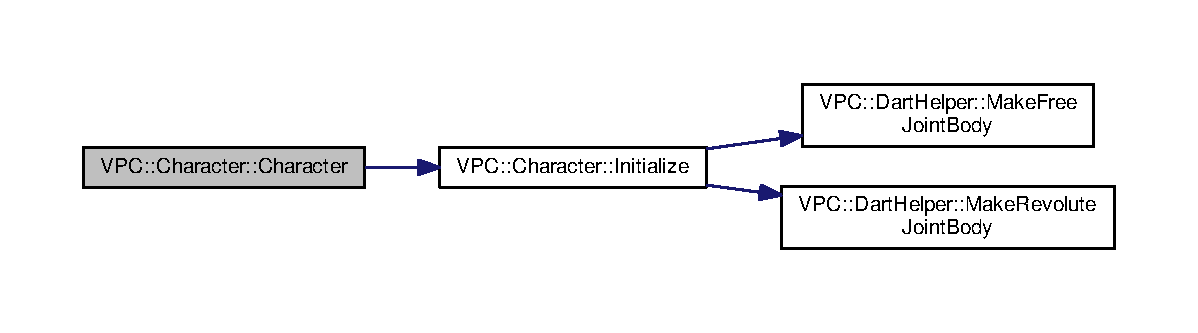
\includegraphics[width=350pt]{class_v_p_c_1_1_character_ab07d09bda7da4df08877ba8a82aed689_cgraph}
\end{center}
\end{figure}




\subsection{Elementa funkcijas dokumentācija}
\index{V\+P\+C\+::\+Character@{V\+P\+C\+::\+Character}!Get\+Skeleton@{Get\+Skeleton}}
\index{Get\+Skeleton@{Get\+Skeleton}!V\+P\+C\+::\+Character@{V\+P\+C\+::\+Character}}
\subsubsection[{\texorpdfstring{Get\+Skeleton()}{GetSkeleton()}}]{\setlength{\rightskip}{0pt plus 5cm}const dart\+::dynamics\+::\+Skeleton\+Ptr\& V\+P\+C\+::\+Character\+::\+Get\+Skeleton (
\begin{DoxyParamCaption}
{}
\end{DoxyParamCaption}
)\hspace{0.3cm}{\ttfamily [inline]}}\hypertarget{class_v_p_c_1_1_character_ab2694f013d033805504228cb151a368f}{}\label{class_v_p_c_1_1_character_ab2694f013d033805504228cb151a368f}


Definēts līnijā 16 failā Character.\+h.


\begin{DoxyCode}
16 \{\textcolor{keywordflow}{return} \hyperlink{class_v_p_c_1_1_character_afbd0d7d0c6227cabd47de1a5c2d7c039}{mSkeleton};\}
\end{DoxyCode}
\index{V\+P\+C\+::\+Character@{V\+P\+C\+::\+Character}!Initialize@{Initialize}}
\index{Initialize@{Initialize}!V\+P\+C\+::\+Character@{V\+P\+C\+::\+Character}}
\subsubsection[{\texorpdfstring{Initialize()}{Initialize()}}]{\setlength{\rightskip}{0pt plus 5cm}void V\+P\+C\+::\+Character\+::\+Initialize (
\begin{DoxyParamCaption}
{}
\end{DoxyParamCaption}
)}\hypertarget{class_v_p_c_1_1_character_a9fb1410736359fab3877e3afe18f2877}{}\label{class_v_p_c_1_1_character_a9fb1410736359fab3877e3afe18f2877}


Definēts līnijā 16 failā Character.\+cpp.


\begin{DoxyCode}
17 \{
18     \hyperlink{class_v_p_c_1_1_character_afbd0d7d0c6227cabd47de1a5c2d7c039}{mSkeleton} = Skeleton::create(\hyperlink{class_v_p_c_1_1_character_a66b5e53cb1779993ae7b78e1b29209b5}{mName});
19 \textcolor{comment}{//  auto cart = DartHelper::MakePrismaticJointBody(}
20 \textcolor{comment}{//      "Cart",}
21 \textcolor{comment}{//      mSkeleton,}
22 \textcolor{comment}{//      nullptr,}
23 \textcolor{comment}{//      Eigen::Vector3d(0.2,0.1,0.1),}
24 \textcolor{comment}{//      Eigen::Vector3d(0,0,0),}
25 \textcolor{comment}{//      Eigen::Vector3d(0.0,0.0501,0.0),1.0);}
26 \textcolor{comment}{//}
27 \textcolor{comment}{//  auto pole = DartHelper::MakeRevoluteJointBody(}
28 \textcolor{comment}{//      "Pole",}
29 \textcolor{comment}{//      mSkeleton,}
30 \textcolor{comment}{//      cart,}
31 \textcolor{comment}{//      Eigen::Vector3d(0.05,0.5,0.05),}
32 \textcolor{comment}{//      Eigen::Vector3d(0,0.05,0),}
33 \textcolor{comment}{//      Eigen::Vector3d(0,0.3,0),1.0);}
34 
35 \textcolor{comment}{//   Pole initially tilted}
36 \textcolor{comment}{//    srand(time(NULL));}
37 \textcolor{comment}{//    double angle = rand()%40 - 20;}
38 \textcolor{comment}{//  mSkeleton->setPosition(1,0.001*angle);}
39 
40     \hyperlink{namespace_v_p_c_1_1_dart_helper_a69fa7c63ad96f84bb86411e438a73d48}{DartHelper::MakeFreeJointBody}(
41         \textcolor{stringliteral}{"Torso"},
42         \hyperlink{class_v_p_c_1_1_character_afbd0d7d0c6227cabd47de1a5c2d7c039}{mSkeleton},
43         \textcolor{keyword}{nullptr},
44         Eigen::Vector3d(0.0,0.4,0.2),
45         Eigen::Vector3d(0,1.1,0),
46         70);
47 
48     \hyperlink{namespace_v_p_c_1_1_dart_helper_a4cf2225ca4d44189f0f0f390cf7aff99}{DartHelper::MakeRevoluteJointBody}(
49         \textcolor{stringliteral}{"ThighR"},
50         \hyperlink{class_v_p_c_1_1_character_afbd0d7d0c6227cabd47de1a5c2d7c039}{mSkeleton},
51         \hyperlink{class_v_p_c_1_1_character_afbd0d7d0c6227cabd47de1a5c2d7c039}{mSkeleton}->getBodyNode(\textcolor{stringliteral}{"Torso"}),
52         Eigen::Vector3d(0.0,0.4,0.1),
53         Eigen::Vector3d(-0.0,0.9,0),
54         Eigen::Vector3d(-0.0,0.7,0),
55         5);
56 
57     \hyperlink{namespace_v_p_c_1_1_dart_helper_a4cf2225ca4d44189f0f0f390cf7aff99}{DartHelper::MakeRevoluteJointBody}(
58         \textcolor{stringliteral}{"ThighL"},
59         \hyperlink{class_v_p_c_1_1_character_afbd0d7d0c6227cabd47de1a5c2d7c039}{mSkeleton},
60         \hyperlink{class_v_p_c_1_1_character_afbd0d7d0c6227cabd47de1a5c2d7c039}{mSkeleton}->getBodyNode(\textcolor{stringliteral}{"Torso"}),
61         Eigen::Vector3d(0.0,0.4,0.1),
62         Eigen::Vector3d(0.0,0.9,0),
63         Eigen::Vector3d(0.0,0.7,0),
64         5);
65 
66     \hyperlink{namespace_v_p_c_1_1_dart_helper_a4cf2225ca4d44189f0f0f390cf7aff99}{DartHelper::MakeRevoluteJointBody}(
67         \textcolor{stringliteral}{"KneeR"},
68         \hyperlink{class_v_p_c_1_1_character_afbd0d7d0c6227cabd47de1a5c2d7c039}{mSkeleton},
69         \hyperlink{class_v_p_c_1_1_character_afbd0d7d0c6227cabd47de1a5c2d7c039}{mSkeleton}->getBodyNode(\textcolor{stringliteral}{"ThighR"}),
70         Eigen::Vector3d(0.0,0.4,0.1),
71         Eigen::Vector3d(-0.0,0.5,0),
72         Eigen::Vector3d(-0.0,0.3,0),
73         4);
74 
75     \hyperlink{namespace_v_p_c_1_1_dart_helper_a4cf2225ca4d44189f0f0f390cf7aff99}{DartHelper::MakeRevoluteJointBody}(
76         \textcolor{stringliteral}{"KneeL"},
77         \hyperlink{class_v_p_c_1_1_character_afbd0d7d0c6227cabd47de1a5c2d7c039}{mSkeleton},
78         \hyperlink{class_v_p_c_1_1_character_afbd0d7d0c6227cabd47de1a5c2d7c039}{mSkeleton}->getBodyNode(\textcolor{stringliteral}{"ThighL"}),
79         Eigen::Vector3d(0.0,0.4,0.1),
80         Eigen::Vector3d(0.0,0.5,0),
81         Eigen::Vector3d(0.0,0.3,0),
82         4);
83 
84     \hyperlink{namespace_v_p_c_1_1_dart_helper_a4cf2225ca4d44189f0f0f390cf7aff99}{DartHelper::MakeRevoluteJointBody}(
85         \textcolor{stringliteral}{"FootR"},
86         \hyperlink{class_v_p_c_1_1_character_afbd0d7d0c6227cabd47de1a5c2d7c039}{mSkeleton},
87         \hyperlink{class_v_p_c_1_1_character_afbd0d7d0c6227cabd47de1a5c2d7c039}{mSkeleton}->getBodyNode(\textcolor{stringliteral}{"KneeR"}),
88         Eigen::Vector3d(0.0,0.095,0.2),
89         Eigen::Vector3d(-0.0,0.1,0),
90         Eigen::Vector3d(-0.0,0.05,-0.03),
91         1);
92 
93     \hyperlink{namespace_v_p_c_1_1_dart_helper_a4cf2225ca4d44189f0f0f390cf7aff99}{DartHelper::MakeRevoluteJointBody}(
94         \textcolor{stringliteral}{"FootL"},
95         \hyperlink{class_v_p_c_1_1_character_afbd0d7d0c6227cabd47de1a5c2d7c039}{mSkeleton},
96         \hyperlink{class_v_p_c_1_1_character_afbd0d7d0c6227cabd47de1a5c2d7c039}{mSkeleton}->getBodyNode(\textcolor{stringliteral}{"KneeL"}),
97         Eigen::Vector3d(0.0,0.095,0.2),
98         Eigen::Vector3d(0.0,0.1,0),
99         Eigen::Vector3d(0.0,0.05,-0.03),
100         1);
101 
102 
103 
104 
105 
106 
107     \textcolor{comment}{// DartHelper::MakeFreeJointBody(}
108     \textcolor{comment}{//  "Torso",}
109     \textcolor{comment}{//  mSkeleton,}
110     \textcolor{comment}{//  nullptr,}
111     \textcolor{comment}{//  Eigen::Vector3d(0.4,0.4,0.2),}
112     \textcolor{comment}{//  Eigen::Vector3d(0,1.1,0),}
113     \textcolor{comment}{//  70);}
114 
115     \textcolor{comment}{// DartHelper::MakeRevoluteJointBody(}
116     \textcolor{comment}{//  "ThighR",}
117     \textcolor{comment}{//  mSkeleton,}
118     \textcolor{comment}{//  mSkeleton->getBodyNode("Torso"),}
119     \textcolor{comment}{//  Eigen::Vector3d(0.1,0.4,0.1),}
120     \textcolor{comment}{//  Eigen::Vector3d(-0.2,0.9,0),}
121     \textcolor{comment}{//  Eigen::Vector3d(-0.2,0.7,0),}
122     \textcolor{comment}{//  5);}
123 
124     \textcolor{comment}{// DartHelper::MakeRevoluteJointBody(}
125     \textcolor{comment}{//  "ThighL",}
126     \textcolor{comment}{//  mSkeleton,}
127     \textcolor{comment}{//  mSkeleton->getBodyNode("Torso"),}
128     \textcolor{comment}{//  Eigen::Vector3d(0.1,0.4,0.1),}
129     \textcolor{comment}{//  Eigen::Vector3d(0.2,0.9,0),}
130     \textcolor{comment}{//  Eigen::Vector3d(0.2,0.7,0),}
131     \textcolor{comment}{//  5);}
132 
133     \textcolor{comment}{// DartHelper::MakeRevoluteJointBody(}
134     \textcolor{comment}{//  "KneeR",}
135     \textcolor{comment}{//  mSkeleton,}
136     \textcolor{comment}{//  mSkeleton->getBodyNode("ThighR"),}
137     \textcolor{comment}{//  Eigen::Vector3d(0.1,0.4,0.1),}
138     \textcolor{comment}{//  Eigen::Vector3d(-0.2,0.5,0),}
139     \textcolor{comment}{//  Eigen::Vector3d(-0.2,0.3,0),}
140     \textcolor{comment}{//  4);}
141 
142     \textcolor{comment}{// DartHelper::MakeRevoluteJointBody(}
143     \textcolor{comment}{//  "KneeL",}
144     \textcolor{comment}{//  mSkeleton,}
145     \textcolor{comment}{//  mSkeleton->getBodyNode("ThighL"),}
146     \textcolor{comment}{//  Eigen::Vector3d(0.1,0.4,0.1),}
147     \textcolor{comment}{//  Eigen::Vector3d(0.2,0.5,0),}
148     \textcolor{comment}{//  Eigen::Vector3d(0.2,0.3,0),}
149     \textcolor{comment}{//  4);}
150 
151     \textcolor{comment}{// DartHelper::MakeRevoluteJointBody(}
152     \textcolor{comment}{//  "FootR",}
153     \textcolor{comment}{//  mSkeleton,}
154     \textcolor{comment}{//  mSkeleton->getBodyNode("KneeR"),}
155     \textcolor{comment}{//  Eigen::Vector3d(0.2,0.1,0.3),}
156     \textcolor{comment}{//  Eigen::Vector3d(-0.2,0.1,0),}
157     \textcolor{comment}{//  Eigen::Vector3d(-0.2,0.05,0.07),}
158     \textcolor{comment}{//  1);}
159 
160     \textcolor{comment}{// DartHelper::MakeBallJointBody(}
161     \textcolor{comment}{//  "FootL",}
162     \textcolor{comment}{//  mSkeleton,}
163     \textcolor{comment}{//  mSkeleton->getBodyNode("KneeL"),}
164     \textcolor{comment}{//  Eigen::Vector3d(0.2,0.1,0.3),}
165     \textcolor{comment}{//  Eigen::Vector3d(0.2,0.1,0),}
166     \textcolor{comment}{//  Eigen::Vector3d(0.2,0.05,0.07),}
167     \textcolor{comment}{//  1);}
168 \}
\end{DoxyCode}


Šeit ir visu funkciju izsaugumu grafs\+:
\nopagebreak
\begin{figure}[H]
\begin{center}
\leavevmode
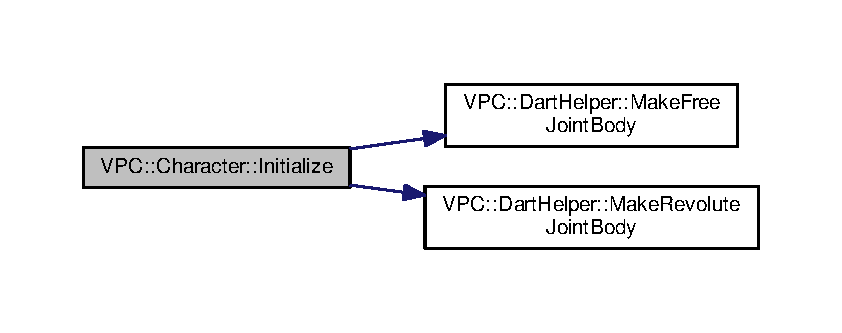
\includegraphics[width=350pt]{class_v_p_c_1_1_character_a9fb1410736359fab3877e3afe18f2877_cgraph}
\end{center}
\end{figure}




Šeit ir šīs funkcijas izsaukuma grafs\+:
\nopagebreak
\begin{figure}[H]
\begin{center}
\leavevmode
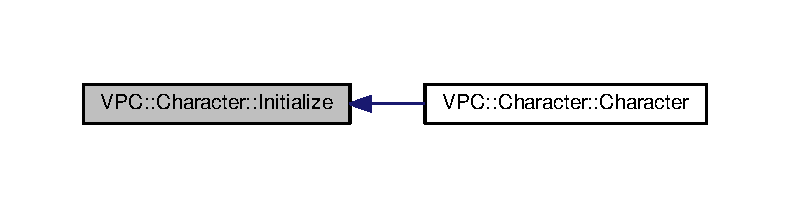
\includegraphics[width=350pt]{class_v_p_c_1_1_character_a9fb1410736359fab3877e3afe18f2877_icgraph}
\end{center}
\end{figure}




\subsection{Elementa datu dokumentācija}
\index{V\+P\+C\+::\+Character@{V\+P\+C\+::\+Character}!m\+Name@{m\+Name}}
\index{m\+Name@{m\+Name}!V\+P\+C\+::\+Character@{V\+P\+C\+::\+Character}}
\subsubsection[{\texorpdfstring{m\+Name}{mName}}]{\setlength{\rightskip}{0pt plus 5cm}std\+::string V\+P\+C\+::\+Character\+::m\+Name\hspace{0.3cm}{\ttfamily [private]}}\hypertarget{class_v_p_c_1_1_character_a66b5e53cb1779993ae7b78e1b29209b5}{}\label{class_v_p_c_1_1_character_a66b5e53cb1779993ae7b78e1b29209b5}


Definēts līnijā 10 failā Character.\+h.

\index{V\+P\+C\+::\+Character@{V\+P\+C\+::\+Character}!m\+Skeleton@{m\+Skeleton}}
\index{m\+Skeleton@{m\+Skeleton}!V\+P\+C\+::\+Character@{V\+P\+C\+::\+Character}}
\subsubsection[{\texorpdfstring{m\+Skeleton}{mSkeleton}}]{\setlength{\rightskip}{0pt plus 5cm}dart\+::dynamics\+::\+Skeleton\+Ptr V\+P\+C\+::\+Character\+::m\+Skeleton\hspace{0.3cm}{\ttfamily [private]}}\hypertarget{class_v_p_c_1_1_character_afbd0d7d0c6227cabd47de1a5c2d7c039}{}\label{class_v_p_c_1_1_character_afbd0d7d0c6227cabd47de1a5c2d7c039}


Definēts līnijā 11 failā Character.\+h.



Šīs klases dokumentācijas tika ģenerēta no šāda failiem\+:\begin{DoxyCompactItemize}
\item 
engine/\hyperlink{_character_8h}{Character.\+h}\item 
engine/\hyperlink{_character_8cpp}{Character.\+cpp}\end{DoxyCompactItemize}

\hypertarget{class_v_p_c_1_1_controller}{}\section{V\+PC\+:\+:Controller klases apraksts}
\label{class_v_p_c_1_1_controller}\index{V\+P\+C\+::\+Controller@{V\+P\+C\+::\+Controller}}


{\ttfamily \#include $<$Controller.\+h$>$}



Sadarbības diagramma klasei V\+PC\+:\+:Controller\+:
\nopagebreak
\begin{figure}[H]
\begin{center}
\leavevmode
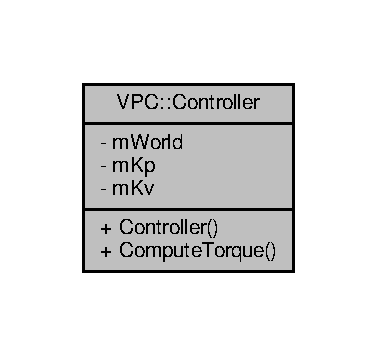
\includegraphics[width=181pt]{class_v_p_c_1_1_controller__coll__graph}
\end{center}
\end{figure}
\subsection*{Publiskās elementa funkcijas}
\begin{DoxyCompactItemize}
\item 
\hyperlink{class_v_p_c_1_1_controller_a132b5d8ac47550346fecf84fe8008179}{Controller} (const std\+::shared\+\_\+ptr$<$ \hyperlink{class_v_p_c_1_1_world}{V\+P\+C\+::\+World} $>$ \&world)
\item 
Eigen\+::\+Vector\+Xd \hyperlink{class_v_p_c_1_1_controller_a15c395dff986eed594d3f99d58e7d3d1}{Compute\+Torque} (const Eigen\+::\+Vector\+Xd \&p, const Eigen\+::\+Vector\+Xd \&v)
\end{DoxyCompactItemize}
\subsection*{Privātie atribūti}
\begin{DoxyCompactItemize}
\item 
std\+::shared\+\_\+ptr$<$ \hyperlink{class_v_p_c_1_1_world}{V\+P\+C\+::\+World} $>$ \hyperlink{class_v_p_c_1_1_controller_a9c46fee9b19ef4f4d79726717f923586}{m\+World}
\item 
Eigen\+::\+Vector\+Xd \hyperlink{class_v_p_c_1_1_controller_a88da6e3301abaeb5b63fd1519fb67cb1}{m\+Kp}
\item 
Eigen\+::\+Vector\+Xd \hyperlink{class_v_p_c_1_1_controller_a6c4a4f388d7ee81f2519e4b05f653f9d}{m\+Kv}
\end{DoxyCompactItemize}


\subsection{Detalizēts apraksts}


Definēts līnijā 7 failā Controller.\+h.



\subsection{Konstruktora un destruktora dokumentācija}
\index{V\+P\+C\+::\+Controller@{V\+P\+C\+::\+Controller}!Controller@{Controller}}
\index{Controller@{Controller}!V\+P\+C\+::\+Controller@{V\+P\+C\+::\+Controller}}
\subsubsection[{\texorpdfstring{Controller(const std\+::shared\+\_\+ptr$<$ V\+P\+C\+::\+World $>$ \&world)}{Controller(const std::shared_ptr< VPC::World > &world)}}]{\setlength{\rightskip}{0pt plus 5cm}V\+P\+C\+::\+Controller\+::\+Controller (
\begin{DoxyParamCaption}
\item[{const std\+::shared\+\_\+ptr$<$ {\bf V\+P\+C\+::\+World} $>$ \&}]{world}
\end{DoxyParamCaption}
)}\hypertarget{class_v_p_c_1_1_controller_a132b5d8ac47550346fecf84fe8008179}{}\label{class_v_p_c_1_1_controller_a132b5d8ac47550346fecf84fe8008179}


Definēts līnijā 6 failā Controller.\+cpp.


\begin{DoxyCode}
7     :\hyperlink{class_v_p_c_1_1_controller_a9c46fee9b19ef4f4d79726717f923586}{mWorld}(world)
8 \{
9     \textcolor{keyword}{auto}& skel =\hyperlink{class_v_p_c_1_1_controller_a9c46fee9b19ef4f4d79726717f923586}{mWorld}->GetCharacter()->GetSkeleton();
10     \hyperlink{class_v_p_c_1_1_controller_a6c4a4f388d7ee81f2519e4b05f653f9d}{mKv} = Eigen::VectorXd::Zero(skel->getNumDofs());
11     \hyperlink{class_v_p_c_1_1_controller_a88da6e3301abaeb5b63fd1519fb67cb1}{mKp} = Eigen::VectorXd::Zero(skel->getNumDofs());
12 
13 
14     \textcolor{keywordtype}{int} start\_index = skel->getBodyNode(1)->getParentJoint()->getIndexInSkeleton(0);
15     \textcolor{comment}{// mKp.block<3,1>(6,0) = Eigen::Vector3d::Constant(50);}
16     \textcolor{comment}{// mKp.block<3,1>(9,0) = Eigen::Vector3d::Constant(50);}
17 
18     \textcolor{comment}{// mKp.block<3,1>(12,0) = Eigen::Vector3d::Constant(10);}
19     \textcolor{comment}{// mKp.block<3,1>(15,0) = Eigen::Vector3d::Constant(10);}
20 
21     \textcolor{comment}{// mKp.block<3,1>(18,0) = Eigen::Vector3d::Constant(10);}
22     \textcolor{comment}{// mKp.block<3,1>(21,0) = Eigen::Vector3d::Constant(10);}
23     mKp = Eigen::VectorXd::Constant(skel->getNumDofs(),300);
24     \hyperlink{class_v_p_c_1_1_controller_a6c4a4f388d7ee81f2519e4b05f653f9d}{mKv} = Eigen::VectorXd::Constant(skel->getNumDofs(),30);
25     \textcolor{comment}{// mKp.tail(skel->getNumDofs()-start\_index) =
       Eigen::VectorXd::Constant(skel->getNumDofs()-start\_index,300);}
26     \textcolor{comment}{// mKv.tail(skel->getNumDofs()-start\_index) =
       Eigen::VectorXd::Constant(skel->getNumDofs()-start\_index,30);}
27 \}
\end{DoxyCode}


Šeit ir visu funkciju izsaugumu grafs\+:
\nopagebreak
\begin{figure}[H]
\begin{center}
\leavevmode
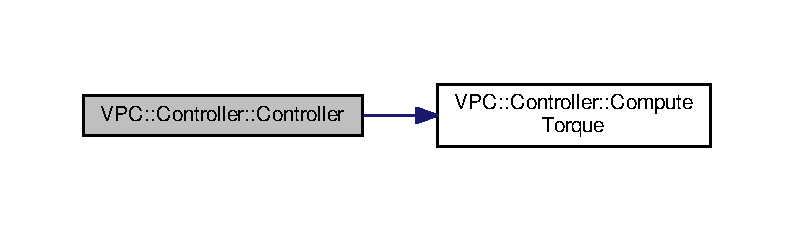
\includegraphics[width=350pt]{class_v_p_c_1_1_controller_a132b5d8ac47550346fecf84fe8008179_cgraph}
\end{center}
\end{figure}




\subsection{Elementa funkcijas dokumentācija}
\index{V\+P\+C\+::\+Controller@{V\+P\+C\+::\+Controller}!Compute\+Torque@{Compute\+Torque}}
\index{Compute\+Torque@{Compute\+Torque}!V\+P\+C\+::\+Controller@{V\+P\+C\+::\+Controller}}
\subsubsection[{\texorpdfstring{Compute\+Torque(const Eigen\+::\+Vector\+Xd \&p, const Eigen\+::\+Vector\+Xd \&v)}{ComputeTorque(const Eigen::VectorXd &p, const Eigen::VectorXd &v)}}]{\setlength{\rightskip}{0pt plus 5cm}Eigen\+::\+Vector\+Xd V\+P\+C\+::\+Controller\+::\+Compute\+Torque (
\begin{DoxyParamCaption}
\item[{const Eigen\+::\+Vector\+Xd \&}]{p, }
\item[{const Eigen\+::\+Vector\+Xd \&}]{v}
\end{DoxyParamCaption}
)}\hypertarget{class_v_p_c_1_1_controller_a15c395dff986eed594d3f99d58e7d3d1}{}\label{class_v_p_c_1_1_controller_a15c395dff986eed594d3f99d58e7d3d1}


Definēts līnijā 30 failā Controller.\+cpp.


\begin{DoxyCode}
31 \{
32     \textcolor{keyword}{auto}& skel =\hyperlink{class_v_p_c_1_1_controller_a9c46fee9b19ef4f4d79726717f923586}{mWorld}->GetCharacter()->GetSkeleton();
33     Eigen::VectorXd p\_diff = skel->getPositionDifferences(p,skel->getPositions());
34     Eigen::VectorXd v\_diff = v - skel->getVelocities();
35     Eigen::VectorXd tau = \hyperlink{class_v_p_c_1_1_controller_a88da6e3301abaeb5b63fd1519fb67cb1}{mKp}.cwiseProduct(p\_diff) + \hyperlink{class_v_p_c_1_1_controller_a6c4a4f388d7ee81f2519e4b05f653f9d}{mKv}.cwiseProduct(v\_diff);
36     \textcolor{keywordflow}{return} tau;
37 \}
\end{DoxyCode}


Šeit ir šīs funkcijas izsaukuma grafs\+:
\nopagebreak
\begin{figure}[H]
\begin{center}
\leavevmode
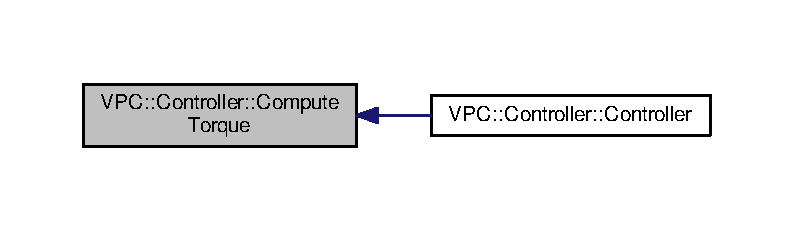
\includegraphics[width=350pt]{class_v_p_c_1_1_controller_a15c395dff986eed594d3f99d58e7d3d1_icgraph}
\end{center}
\end{figure}




\subsection{Elementa datu dokumentācija}
\index{V\+P\+C\+::\+Controller@{V\+P\+C\+::\+Controller}!m\+Kp@{m\+Kp}}
\index{m\+Kp@{m\+Kp}!V\+P\+C\+::\+Controller@{V\+P\+C\+::\+Controller}}
\subsubsection[{\texorpdfstring{m\+Kp}{mKp}}]{\setlength{\rightskip}{0pt plus 5cm}Eigen\+::\+Vector\+Xd V\+P\+C\+::\+Controller\+::m\+Kp\hspace{0.3cm}{\ttfamily [private]}}\hypertarget{class_v_p_c_1_1_controller_a88da6e3301abaeb5b63fd1519fb67cb1}{}\label{class_v_p_c_1_1_controller_a88da6e3301abaeb5b63fd1519fb67cb1}


Definēts līnijā 11 failā Controller.\+h.

\index{V\+P\+C\+::\+Controller@{V\+P\+C\+::\+Controller}!m\+Kv@{m\+Kv}}
\index{m\+Kv@{m\+Kv}!V\+P\+C\+::\+Controller@{V\+P\+C\+::\+Controller}}
\subsubsection[{\texorpdfstring{m\+Kv}{mKv}}]{\setlength{\rightskip}{0pt plus 5cm}Eigen\+::\+Vector\+Xd V\+P\+C\+::\+Controller\+::m\+Kv\hspace{0.3cm}{\ttfamily [private]}}\hypertarget{class_v_p_c_1_1_controller_a6c4a4f388d7ee81f2519e4b05f653f9d}{}\label{class_v_p_c_1_1_controller_a6c4a4f388d7ee81f2519e4b05f653f9d}


Definēts līnijā 11 failā Controller.\+h.

\index{V\+P\+C\+::\+Controller@{V\+P\+C\+::\+Controller}!m\+World@{m\+World}}
\index{m\+World@{m\+World}!V\+P\+C\+::\+Controller@{V\+P\+C\+::\+Controller}}
\subsubsection[{\texorpdfstring{m\+World}{mWorld}}]{\setlength{\rightskip}{0pt plus 5cm}std\+::shared\+\_\+ptr$<${\bf V\+P\+C\+::\+World}$>$ V\+P\+C\+::\+Controller\+::m\+World\hspace{0.3cm}{\ttfamily [private]}}\hypertarget{class_v_p_c_1_1_controller_a9c46fee9b19ef4f4d79726717f923586}{}\label{class_v_p_c_1_1_controller_a9c46fee9b19ef4f4d79726717f923586}


Definēts līnijā 10 failā Controller.\+h.



Šīs klases dokumentācijas tika ģenerēta no šāda failiem\+:\begin{DoxyCompactItemize}
\item 
engine/\hyperlink{_controller_8h}{Controller.\+h}\item 
engine/\hyperlink{_controller_8cpp}{Controller.\+cpp}\end{DoxyCompactItemize}

\hypertarget{classddpg__others_1_1_critic}{}\section{ddpg\+\_\+others.\+Critic klases apraksts}
\label{classddpg__others_1_1_critic}\index{ddpg\+\_\+others.\+Critic@{ddpg\+\_\+others.\+Critic}}


Mantojamības diagramma klasei ddpg\+\_\+others.\+Critic\+:
\nopagebreak
\begin{figure}[H]
\begin{center}
\leavevmode
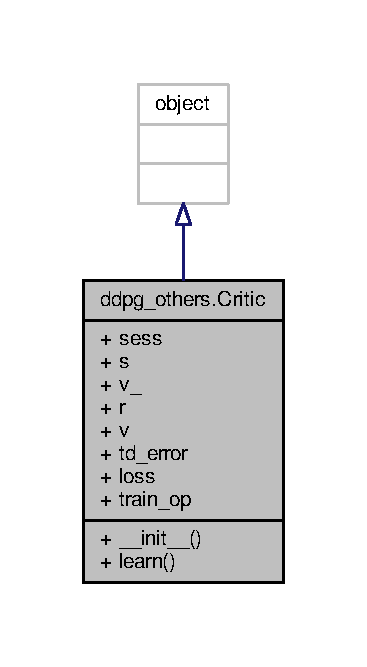
\includegraphics[width=176pt]{classddpg__others_1_1_critic__inherit__graph}
\end{center}
\end{figure}


Sadarbības diagramma klasei ddpg\+\_\+others.\+Critic\+:
\nopagebreak
\begin{figure}[H]
\begin{center}
\leavevmode
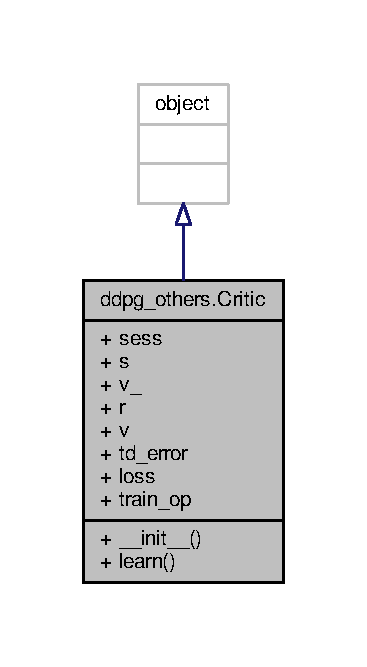
\includegraphics[width=176pt]{classddpg__others_1_1_critic__coll__graph}
\end{center}
\end{figure}
\subsection*{Publiskās elementa funkcijas}
\begin{DoxyCompactItemize}
\item 
def \hyperlink{classddpg__others_1_1_critic_ad79f6a3961bf9da84b50feb690f72708}{\+\_\+\+\_\+init\+\_\+\+\_\+} (self, \hyperlink{classddpg__others_1_1_critic_ab0c8a33f283df68173a93990084034de}{sess}, n\+\_\+features, lr=0.\+01)
\item 
def \hyperlink{classddpg__others_1_1_critic_aa108c309d56a4e946e76908168a97cdf}{learn} (self, \hyperlink{classddpg__others_1_1_critic_a6d70d80341ad76c8c12ddaf0e06e513a}{s}, \hyperlink{classddpg__others_1_1_critic_a127f5c9ec25bd223417b5f478bc2a11f}{r}, \hyperlink{namespaceddpg__others_a9401d5decfd243fdd11c64d512501ff1}{s\+\_\+})
\end{DoxyCompactItemize}
\subsection*{Publiskie atribūti}
\begin{DoxyCompactItemize}
\item 
\hyperlink{classddpg__others_1_1_critic_ab0c8a33f283df68173a93990084034de}{sess}
\item 
\hyperlink{classddpg__others_1_1_critic_a6d70d80341ad76c8c12ddaf0e06e513a}{s}
\item 
\hyperlink{classddpg__others_1_1_critic_a44cb021fd77cfeb1515d1421ea1135cd}{v\+\_\+}
\item 
\hyperlink{classddpg__others_1_1_critic_a127f5c9ec25bd223417b5f478bc2a11f}{r}
\item 
\hyperlink{classddpg__others_1_1_critic_a4ea207b84e027e537185c3067f21e8fd}{v}
\item 
\hyperlink{classddpg__others_1_1_critic_acd08db4e575e41c9b40c89aeb70b69fc}{td\+\_\+error}
\item 
\hyperlink{classddpg__others_1_1_critic_a234f0de11677fd4cc6b2387173ed5065}{loss}
\item 
\hyperlink{classddpg__others_1_1_critic_a3c9fc0fa915bdd1c961e8a94b60e486f}{train\+\_\+op}
\end{DoxyCompactItemize}


\subsection{Detalizēts apraksts}


Definēts līnijā 84 failā ddpg\+\_\+others.\+py.



\subsection{Konstruktora un destruktora dokumentācija}
\index{ddpg\+\_\+others\+::\+Critic@{ddpg\+\_\+others\+::\+Critic}!\+\_\+\+\_\+init\+\_\+\+\_\+@{\+\_\+\+\_\+init\+\_\+\+\_\+}}
\index{\+\_\+\+\_\+init\+\_\+\+\_\+@{\+\_\+\+\_\+init\+\_\+\+\_\+}!ddpg\+\_\+others\+::\+Critic@{ddpg\+\_\+others\+::\+Critic}}
\subsubsection[{\texorpdfstring{\+\_\+\+\_\+init\+\_\+\+\_\+(self, sess, n\+\_\+features, lr=0.\+01)}{__init__(self, sess, n_features, lr=0.01)}}]{\setlength{\rightskip}{0pt plus 5cm}def ddpg\+\_\+others.\+Critic.\+\_\+\+\_\+init\+\_\+\+\_\+ (
\begin{DoxyParamCaption}
\item[{}]{self, }
\item[{}]{sess, }
\item[{}]{n\+\_\+features, }
\item[{}]{lr = {\ttfamily 0.01}}
\end{DoxyParamCaption}
)}\hypertarget{classddpg__others_1_1_critic_ad79f6a3961bf9da84b50feb690f72708}{}\label{classddpg__others_1_1_critic_ad79f6a3961bf9da84b50feb690f72708}


Definēts līnijā 85 failā ddpg\+\_\+others.\+py.


\begin{DoxyCode}
85     \textcolor{keyword}{def }\hyperlink{classddpg__others_1_1_critic_ad79f6a3961bf9da84b50feb690f72708}{\_\_init\_\_}(self, sess, n\_features, lr=0.01):
86         self.\hyperlink{classddpg__others_1_1_critic_ab0c8a33f283df68173a93990084034de}{sess} = sess
87         with tf.name\_scope(\textcolor{stringliteral}{'inputs'}):
88             self.\hyperlink{classddpg__others_1_1_critic_a6d70d80341ad76c8c12ddaf0e06e513a}{s} = tf.placeholder(tf.float32, [1, n\_features], \textcolor{stringliteral}{"state"})
89             self.\hyperlink{classddpg__others_1_1_critic_a44cb021fd77cfeb1515d1421ea1135cd}{v\_} = tf.placeholder(tf.float32, [1, 1], name=\textcolor{stringliteral}{"v\_next"})
90             self.\hyperlink{classddpg__others_1_1_critic_a127f5c9ec25bd223417b5f478bc2a11f}{r} = tf.placeholder(tf.float32, name=\textcolor{stringliteral}{'r')}
91 \textcolor{stringliteral}{}
92 \textcolor{stringliteral}{        with tf.variable\_scope('Critic'}):
93             l1 = tf.layers.dense(
94                 inputs=self.\hyperlink{classddpg__others_1_1_critic_a6d70d80341ad76c8c12ddaf0e06e513a}{s},
95                 units=30,  \textcolor{comment}{# number of hidden units}
96                 activation=tf.nn.relu,
97                 kernel\_initializer=tf.random\_normal\_initializer(0., .1),  \textcolor{comment}{# weights}
98                 bias\_initializer=tf.constant\_initializer(0.1),  \textcolor{comment}{# biases}
99                 name=\textcolor{stringliteral}{'l1'}
100             )
101 
102             self.\hyperlink{classddpg__others_1_1_critic_a4ea207b84e027e537185c3067f21e8fd}{v} = tf.layers.dense(
103                 inputs=l1,
104                 units=1,  \textcolor{comment}{# output units}
105                 activation=\textcolor{keywordtype}{None},
106                 kernel\_initializer=tf.random\_normal\_initializer(0., .1),  \textcolor{comment}{# weights}
107                 bias\_initializer=tf.constant\_initializer(0.1),  \textcolor{comment}{# biases}
108                 name=\textcolor{stringliteral}{'V'}
109             )
110 
111         with tf.variable\_scope(\textcolor{stringliteral}{'squared\_TD\_error'}):
112             self.\hyperlink{classddpg__others_1_1_critic_acd08db4e575e41c9b40c89aeb70b69fc}{td\_error} = tf.reduce\_mean(self.\hyperlink{classddpg__others_1_1_critic_a127f5c9ec25bd223417b5f478bc2a11f}{r} + GAMMA * self.\hyperlink{classddpg__others_1_1_critic_a44cb021fd77cfeb1515d1421ea1135cd}{v\_} - self.
      \hyperlink{classddpg__others_1_1_critic_a4ea207b84e027e537185c3067f21e8fd}{v})
113             self.\hyperlink{classddpg__others_1_1_critic_a234f0de11677fd4cc6b2387173ed5065}{loss} = tf.square(self.\hyperlink{classddpg__others_1_1_critic_acd08db4e575e41c9b40c89aeb70b69fc}{td\_error})    \textcolor{comment}{# TD\_error = (r+gamma*V\_next) - V\_eval}
114         with tf.variable\_scope(\textcolor{stringliteral}{'train'}):
115             self.\hyperlink{classddpg__others_1_1_critic_a3c9fc0fa915bdd1c961e8a94b60e486f}{train\_op} = tf.train.AdamOptimizer(lr).minimize(self.
      \hyperlink{classddpg__others_1_1_critic_a234f0de11677fd4cc6b2387173ed5065}{loss})
116 
\end{DoxyCode}


\subsection{Elementa funkcijas dokumentācija}
\index{ddpg\+\_\+others\+::\+Critic@{ddpg\+\_\+others\+::\+Critic}!learn@{learn}}
\index{learn@{learn}!ddpg\+\_\+others\+::\+Critic@{ddpg\+\_\+others\+::\+Critic}}
\subsubsection[{\texorpdfstring{learn(self, s, r, s\+\_\+)}{learn(self, s, r, s_)}}]{\setlength{\rightskip}{0pt plus 5cm}def ddpg\+\_\+others.\+Critic.\+learn (
\begin{DoxyParamCaption}
\item[{}]{self, }
\item[{}]{s, }
\item[{}]{r, }
\item[{}]{s\+\_\+}
\end{DoxyParamCaption}
)}\hypertarget{classddpg__others_1_1_critic_aa108c309d56a4e946e76908168a97cdf}{}\label{classddpg__others_1_1_critic_aa108c309d56a4e946e76908168a97cdf}


Definēts līnijā 117 failā ddpg\+\_\+others.\+py.


\begin{DoxyCode}
117     \textcolor{keyword}{def }\hyperlink{classddpg__others_1_1_critic_aa108c309d56a4e946e76908168a97cdf}{learn}(self, s, r, s\_):
118         s, s\_ = s[np.newaxis, :], s\_[np.newaxis, :]
119 
120         v\_ = self.sess.run(self.\hyperlink{classddpg__others_1_1_critic_a4ea207b84e027e537185c3067f21e8fd}{v}, \{self.\hyperlink{classddpg__others_1_1_critic_a6d70d80341ad76c8c12ddaf0e06e513a}{s}: s\_\})
121         td\_error, \_ = self.sess.run([self.\hyperlink{classddpg__others_1_1_critic_acd08db4e575e41c9b40c89aeb70b69fc}{td\_error}, self.\hyperlink{classddpg__others_1_1_critic_a3c9fc0fa915bdd1c961e8a94b60e486f}{train\_op}],
122                                     \{self.\hyperlink{classddpg__others_1_1_critic_a6d70d80341ad76c8c12ddaf0e06e513a}{s}: s, self.\hyperlink{classddpg__others_1_1_critic_a44cb021fd77cfeb1515d1421ea1135cd}{v\_}: v\_, self.\hyperlink{classddpg__others_1_1_critic_a127f5c9ec25bd223417b5f478bc2a11f}{r}: r\})
123         \textcolor{keywordflow}{return} td\_error
124 
125 
\end{DoxyCode}


\subsection{Elementa datu dokumentācija}
\index{ddpg\+\_\+others\+::\+Critic@{ddpg\+\_\+others\+::\+Critic}!loss@{loss}}
\index{loss@{loss}!ddpg\+\_\+others\+::\+Critic@{ddpg\+\_\+others\+::\+Critic}}
\subsubsection[{\texorpdfstring{loss}{loss}}]{\setlength{\rightskip}{0pt plus 5cm}ddpg\+\_\+others.\+Critic.\+loss}\hypertarget{classddpg__others_1_1_critic_a234f0de11677fd4cc6b2387173ed5065}{}\label{classddpg__others_1_1_critic_a234f0de11677fd4cc6b2387173ed5065}


Definēts līnijā 113 failā ddpg\+\_\+others.\+py.

\index{ddpg\+\_\+others\+::\+Critic@{ddpg\+\_\+others\+::\+Critic}!r@{r}}
\index{r@{r}!ddpg\+\_\+others\+::\+Critic@{ddpg\+\_\+others\+::\+Critic}}
\subsubsection[{\texorpdfstring{r}{r}}]{\setlength{\rightskip}{0pt plus 5cm}ddpg\+\_\+others.\+Critic.\+r}\hypertarget{classddpg__others_1_1_critic_a127f5c9ec25bd223417b5f478bc2a11f}{}\label{classddpg__others_1_1_critic_a127f5c9ec25bd223417b5f478bc2a11f}


Definēts līnijā 90 failā ddpg\+\_\+others.\+py.

\index{ddpg\+\_\+others\+::\+Critic@{ddpg\+\_\+others\+::\+Critic}!s@{s}}
\index{s@{s}!ddpg\+\_\+others\+::\+Critic@{ddpg\+\_\+others\+::\+Critic}}
\subsubsection[{\texorpdfstring{s}{s}}]{\setlength{\rightskip}{0pt plus 5cm}ddpg\+\_\+others.\+Critic.\+s}\hypertarget{classddpg__others_1_1_critic_a6d70d80341ad76c8c12ddaf0e06e513a}{}\label{classddpg__others_1_1_critic_a6d70d80341ad76c8c12ddaf0e06e513a}


Definēts līnijā 88 failā ddpg\+\_\+others.\+py.

\index{ddpg\+\_\+others\+::\+Critic@{ddpg\+\_\+others\+::\+Critic}!sess@{sess}}
\index{sess@{sess}!ddpg\+\_\+others\+::\+Critic@{ddpg\+\_\+others\+::\+Critic}}
\subsubsection[{\texorpdfstring{sess}{sess}}]{\setlength{\rightskip}{0pt plus 5cm}ddpg\+\_\+others.\+Critic.\+sess}\hypertarget{classddpg__others_1_1_critic_ab0c8a33f283df68173a93990084034de}{}\label{classddpg__others_1_1_critic_ab0c8a33f283df68173a93990084034de}


Definēts līnijā 86 failā ddpg\+\_\+others.\+py.

\index{ddpg\+\_\+others\+::\+Critic@{ddpg\+\_\+others\+::\+Critic}!td\+\_\+error@{td\+\_\+error}}
\index{td\+\_\+error@{td\+\_\+error}!ddpg\+\_\+others\+::\+Critic@{ddpg\+\_\+others\+::\+Critic}}
\subsubsection[{\texorpdfstring{td\+\_\+error}{td_error}}]{\setlength{\rightskip}{0pt plus 5cm}ddpg\+\_\+others.\+Critic.\+td\+\_\+error}\hypertarget{classddpg__others_1_1_critic_acd08db4e575e41c9b40c89aeb70b69fc}{}\label{classddpg__others_1_1_critic_acd08db4e575e41c9b40c89aeb70b69fc}


Definēts līnijā 112 failā ddpg\+\_\+others.\+py.

\index{ddpg\+\_\+others\+::\+Critic@{ddpg\+\_\+others\+::\+Critic}!train\+\_\+op@{train\+\_\+op}}
\index{train\+\_\+op@{train\+\_\+op}!ddpg\+\_\+others\+::\+Critic@{ddpg\+\_\+others\+::\+Critic}}
\subsubsection[{\texorpdfstring{train\+\_\+op}{train_op}}]{\setlength{\rightskip}{0pt plus 5cm}ddpg\+\_\+others.\+Critic.\+train\+\_\+op}\hypertarget{classddpg__others_1_1_critic_a3c9fc0fa915bdd1c961e8a94b60e486f}{}\label{classddpg__others_1_1_critic_a3c9fc0fa915bdd1c961e8a94b60e486f}


Definēts līnijā 115 failā ddpg\+\_\+others.\+py.

\index{ddpg\+\_\+others\+::\+Critic@{ddpg\+\_\+others\+::\+Critic}!v@{v}}
\index{v@{v}!ddpg\+\_\+others\+::\+Critic@{ddpg\+\_\+others\+::\+Critic}}
\subsubsection[{\texorpdfstring{v}{v}}]{\setlength{\rightskip}{0pt plus 5cm}ddpg\+\_\+others.\+Critic.\+v}\hypertarget{classddpg__others_1_1_critic_a4ea207b84e027e537185c3067f21e8fd}{}\label{classddpg__others_1_1_critic_a4ea207b84e027e537185c3067f21e8fd}


Definēts līnijā 102 failā ddpg\+\_\+others.\+py.

\index{ddpg\+\_\+others\+::\+Critic@{ddpg\+\_\+others\+::\+Critic}!v\+\_\+@{v\+\_\+}}
\index{v\+\_\+@{v\+\_\+}!ddpg\+\_\+others\+::\+Critic@{ddpg\+\_\+others\+::\+Critic}}
\subsubsection[{\texorpdfstring{v\+\_\+}{v_}}]{\setlength{\rightskip}{0pt plus 5cm}ddpg\+\_\+others.\+Critic.\+v\+\_\+}\hypertarget{classddpg__others_1_1_critic_a44cb021fd77cfeb1515d1421ea1135cd}{}\label{classddpg__others_1_1_critic_a44cb021fd77cfeb1515d1421ea1135cd}


Definēts līnijā 89 failā ddpg\+\_\+others.\+py.



Šīs klases dokumentācijas tika ģenerēta no šāda faila\+:\begin{DoxyCompactItemize}
\item 
py\+\_\+code/\hyperlink{ddpg__others_8py}{ddpg\+\_\+others.\+py}\end{DoxyCompactItemize}

\hypertarget{classcritic_1_1_critic_network}{}\section{critic.\+Critic\+Network klases apraksts}
\label{classcritic_1_1_critic_network}\index{critic.\+Critic\+Network@{critic.\+Critic\+Network}}


Sadarbības diagramma klasei critic.\+Critic\+Network\+:
\nopagebreak
\begin{figure}[H]
\begin{center}
\leavevmode
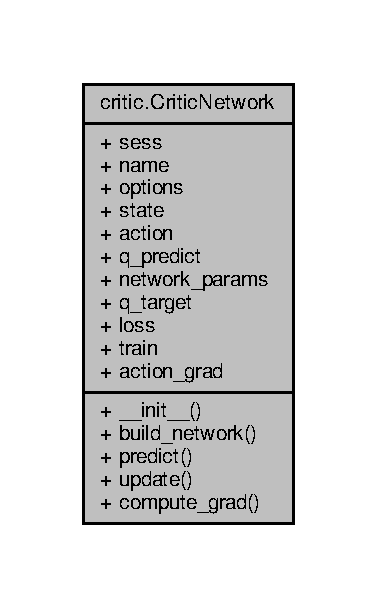
\includegraphics[width=181pt]{classcritic_1_1_critic_network__coll__graph}
\end{center}
\end{figure}
\subsection*{Publiskās elementa funkcijas}
\begin{DoxyCompactItemize}
\item 
def \hyperlink{classcritic_1_1_critic_network_a7f619dd822278ac236b4398003c06f94}{\+\_\+\+\_\+init\+\_\+\+\_\+} (self, \hyperlink{classcritic_1_1_critic_network_ad19c4eb9fce11599a0807f94fcab6343}{sess}, \hyperlink{classcritic_1_1_critic_network_a14fa3b43d18dc2e8e5ca3fcd617b8bcc}{options}, \hyperlink{classcritic_1_1_critic_network_ad7a59dc914d7e6eff3d96c6c819bef38}{name})
\item 
def \hyperlink{classcritic_1_1_critic_network_a6ef997aa35d20b9ff53caa8c87fea17a}{build\+\_\+network} (self)
\item 
def \hyperlink{classcritic_1_1_critic_network_a52b79a3c802070dc8925733bf7dcb42e}{predict} (self, \hyperlink{classcritic_1_1_critic_network_a21da613cb1688ada3b416e4286649fc2}{state}, \hyperlink{classcritic_1_1_critic_network_a78b46c2dc517101434ffc7053581f5a6}{action})
\item 
def \hyperlink{classcritic_1_1_critic_network_af383ed0494f00bb145040d6acdbc6913}{update} (self, states, actions, q\+\_\+targets)
\item 
def \hyperlink{classcritic_1_1_critic_network_aca9bfaf828183ad50b80e971e4de446c}{compute\+\_\+grad} (self, states, actions)
\end{DoxyCompactItemize}
\subsection*{Publiskie atribūti}
\begin{DoxyCompactItemize}
\item 
\hyperlink{classcritic_1_1_critic_network_ad19c4eb9fce11599a0807f94fcab6343}{sess}
\item 
\hyperlink{classcritic_1_1_critic_network_ad7a59dc914d7e6eff3d96c6c819bef38}{name}
\item 
\hyperlink{classcritic_1_1_critic_network_a14fa3b43d18dc2e8e5ca3fcd617b8bcc}{options}
\item 
\hyperlink{classcritic_1_1_critic_network_a21da613cb1688ada3b416e4286649fc2}{state}
\item 
\hyperlink{classcritic_1_1_critic_network_a78b46c2dc517101434ffc7053581f5a6}{action}
\item 
\hyperlink{classcritic_1_1_critic_network_a5c8a5c7b27312a19cd603216db6e5b52}{q\+\_\+predict}
\item 
\hyperlink{classcritic_1_1_critic_network_a033abaa32fa20baf9d2faaa6a2c6fae3}{network\+\_\+params}
\item 
\hyperlink{classcritic_1_1_critic_network_acae4004c3e447aaadc7f25ee2a550f60}{q\+\_\+target}
\item 
\hyperlink{classcritic_1_1_critic_network_a720bbce2d663aea7f91ad957a0d24542}{loss}
\item 
\hyperlink{classcritic_1_1_critic_network_a85b9d34191b5218ce6af960ec3846b4f}{train}
\item 
\hyperlink{classcritic_1_1_critic_network_aeec8c7f1d08044b18a6c85868a18174a}{action\+\_\+grad}
\end{DoxyCompactItemize}


\subsection{Detalizēts apraksts}


Definēts līnijā 4 failā critic.\+py.



\subsection{Konstruktora un destruktora dokumentācija}
\index{critic\+::\+Critic\+Network@{critic\+::\+Critic\+Network}!\+\_\+\+\_\+init\+\_\+\+\_\+@{\+\_\+\+\_\+init\+\_\+\+\_\+}}
\index{\+\_\+\+\_\+init\+\_\+\+\_\+@{\+\_\+\+\_\+init\+\_\+\+\_\+}!critic\+::\+Critic\+Network@{critic\+::\+Critic\+Network}}
\subsubsection[{\texorpdfstring{\+\_\+\+\_\+init\+\_\+\+\_\+(self, sess, options, name)}{__init__(self, sess, options, name)}}]{\setlength{\rightskip}{0pt plus 5cm}def critic.\+Critic\+Network.\+\_\+\+\_\+init\+\_\+\+\_\+ (
\begin{DoxyParamCaption}
\item[{}]{self, }
\item[{}]{sess, }
\item[{}]{options, }
\item[{}]{name}
\end{DoxyParamCaption}
)}\hypertarget{classcritic_1_1_critic_network_a7f619dd822278ac236b4398003c06f94}{}\label{classcritic_1_1_critic_network_a7f619dd822278ac236b4398003c06f94}


Definēts līnijā 5 failā critic.\+py.


\begin{DoxyCode}
5     \textcolor{keyword}{def }\hyperlink{classcritic_1_1_critic_network_a7f619dd822278ac236b4398003c06f94}{\_\_init\_\_}(self,sess,options,name):
6         \textcolor{comment}{# session}
7         \textcolor{comment}{# state\_dim}
8         \textcolor{comment}{# action\_dim}
9         \textcolor{comment}{# learning\_rate}
10         \textcolor{comment}{# name}
11         self.\hyperlink{classcritic_1_1_critic_network_ad19c4eb9fce11599a0807f94fcab6343}{sess} = sess
12         self.\hyperlink{classcritic_1_1_critic_network_ad7a59dc914d7e6eff3d96c6c819bef38}{name} = name
13         self.\hyperlink{classcritic_1_1_critic_network_a14fa3b43d18dc2e8e5ca3fcd617b8bcc}{options} = options
14 
15         self.\hyperlink{classcritic_1_1_critic_network_a6ef997aa35d20b9ff53caa8c87fea17a}{build\_network}()
16 
17         init\_vars = tf.group(tf.global\_variables\_initializer(), tf.local\_variables\_initializer())
18         sess.run(init\_vars)
19 
\end{DoxyCode}


\subsection{Elementa funkcijas dokumentācija}
\index{critic\+::\+Critic\+Network@{critic\+::\+Critic\+Network}!build\+\_\+network@{build\+\_\+network}}
\index{build\+\_\+network@{build\+\_\+network}!critic\+::\+Critic\+Network@{critic\+::\+Critic\+Network}}
\subsubsection[{\texorpdfstring{build\+\_\+network(self)}{build_network(self)}}]{\setlength{\rightskip}{0pt plus 5cm}def critic.\+Critic\+Network.\+build\+\_\+network (
\begin{DoxyParamCaption}
\item[{}]{self}
\end{DoxyParamCaption}
)}\hypertarget{classcritic_1_1_critic_network_a6ef997aa35d20b9ff53caa8c87fea17a}{}\label{classcritic_1_1_critic_network_a6ef997aa35d20b9ff53caa8c87fea17a}


Definēts līnijā 21 failā critic.\+py.


\begin{DoxyCode}
21     \textcolor{keyword}{def }\hyperlink{classcritic_1_1_critic_network_a6ef997aa35d20b9ff53caa8c87fea17a}{build\_network}(self):
22         self.\hyperlink{classcritic_1_1_critic_network_a21da613cb1688ada3b416e4286649fc2}{state} = tf.placeholder(tf.float32, [\textcolor{keywordtype}{None}, self.options.STATE\_DIM]) \textcolor{comment}{# Placeholder}
23         self.\hyperlink{classcritic_1_1_critic_network_a78b46c2dc517101434ffc7053581f5a6}{action} = tf.placeholder(tf.float32, [\textcolor{keywordtype}{None}, self.options.ACTION\_DIM]) \textcolor{comment}{# Placeholder}
24 
25         with tf.variable\_scope(self.\hyperlink{classcritic_1_1_critic_network_ad7a59dc914d7e6eff3d96c6c819bef38}{name}):
26             hidden\_layer\_state = tf.layers.dense(self.\hyperlink{classcritic_1_1_critic_network_a21da613cb1688ada3b416e4286649fc2}{state}, 64, activation = tf.nn.relu, 
      kernel\_initializer = tf.contrib.layers.xavier\_initializer()) \textcolor{comment}{# use elu for hidden layers}
27             \textcolor{comment}{# hidden\_layer\_action = tf.layers.dense(self.action, 16, activation = tf.nn.relu,
       kernel\_initializer = tf.contrib.layers.xavier\_initializer()) # use elu for hidden layers}
28             hidden\_layer\_total = tf.concat([hidden\_layer\_state, self.\hyperlink{classcritic_1_1_critic_network_a78b46c2dc517101434ffc7053581f5a6}{action}], axis=1)
29             hidden\_layer = tf.layers.dense(hidden\_layer\_total, 32, activation = tf.nn.relu, 
      kernel\_initializer=tf.contrib.layers.xavier\_initializer())
30             self.\hyperlink{classcritic_1_1_critic_network_a5c8a5c7b27312a19cd603216db6e5b52}{q\_predict} = tf.layers.dense(hidden\_layer, 1, kernel\_initializer = 
      tf.contrib.layers.xavier\_initializer())
31 
32         self.\hyperlink{classcritic_1_1_critic_network_a033abaa32fa20baf9d2faaa6a2c6fae3}{network\_params} = tf.trainable\_variables(scope = self.
      \hyperlink{classcritic_1_1_critic_network_ad7a59dc914d7e6eff3d96c6c819bef38}{name})
33 
34         self.\hyperlink{classcritic_1_1_critic_network_acae4004c3e447aaadc7f25ee2a550f60}{q\_target} = tf.placeholder(tf.float32, [\textcolor{keywordtype}{None}, 1]) \textcolor{comment}{# Placeholder}
35         self.\hyperlink{classcritic_1_1_critic_network_a720bbce2d663aea7f91ad957a0d24542}{loss} = tf.losses.mean\_squared\_error(self.\hyperlink{classcritic_1_1_critic_network_a5c8a5c7b27312a19cd603216db6e5b52}{q\_predict}, self.
      \hyperlink{classcritic_1_1_critic_network_acae4004c3e447aaadc7f25ee2a550f60}{q\_target})
36         self.\hyperlink{classcritic_1_1_critic_network_a85b9d34191b5218ce6af960ec3846b4f}{train} = tf.train.AdamOptimizer(self.options.LR\_C).minimize(self.
      \hyperlink{classcritic_1_1_critic_network_a720bbce2d663aea7f91ad957a0d24542}{loss})
37 
38         self.\hyperlink{classcritic_1_1_critic_network_aeec8c7f1d08044b18a6c85868a18174a}{action\_grad} = tf.gradients(self.\hyperlink{classcritic_1_1_critic_network_a5c8a5c7b27312a19cd603216db6e5b52}{q\_predict}, self.
      \hyperlink{classcritic_1_1_critic_network_a78b46c2dc517101434ffc7053581f5a6}{action})[0]
39 
\end{DoxyCode}
\index{critic\+::\+Critic\+Network@{critic\+::\+Critic\+Network}!compute\+\_\+grad@{compute\+\_\+grad}}
\index{compute\+\_\+grad@{compute\+\_\+grad}!critic\+::\+Critic\+Network@{critic\+::\+Critic\+Network}}
\subsubsection[{\texorpdfstring{compute\+\_\+grad(self, states, actions)}{compute_grad(self, states, actions)}}]{\setlength{\rightskip}{0pt plus 5cm}def critic.\+Critic\+Network.\+compute\+\_\+grad (
\begin{DoxyParamCaption}
\item[{}]{self, }
\item[{}]{states, }
\item[{}]{actions}
\end{DoxyParamCaption}
)}\hypertarget{classcritic_1_1_critic_network_aca9bfaf828183ad50b80e971e4de446c}{}\label{classcritic_1_1_critic_network_aca9bfaf828183ad50b80e971e4de446c}


Definēts līnijā 57 failā critic.\+py.


\begin{DoxyCode}
57     \textcolor{keyword}{def }\hyperlink{classcritic_1_1_critic_network_aca9bfaf828183ad50b80e971e4de446c}{compute\_grad}(self, states, actions):
58         \textcolor{keywordflow}{return} self.sess.run(self.\hyperlink{classcritic_1_1_critic_network_aeec8c7f1d08044b18a6c85868a18174a}{action\_grad},
59                              feed\_dict=\{
60                                  self.\hyperlink{classcritic_1_1_critic_network_a21da613cb1688ada3b416e4286649fc2}{state}: states,
61                                  self.\hyperlink{classcritic_1_1_critic_network_a78b46c2dc517101434ffc7053581f5a6}{action}: actions
62                              \}\end{DoxyCode}
\index{critic\+::\+Critic\+Network@{critic\+::\+Critic\+Network}!predict@{predict}}
\index{predict@{predict}!critic\+::\+Critic\+Network@{critic\+::\+Critic\+Network}}
\subsubsection[{\texorpdfstring{predict(self, state, action)}{predict(self, state, action)}}]{\setlength{\rightskip}{0pt plus 5cm}def critic.\+Critic\+Network.\+predict (
\begin{DoxyParamCaption}
\item[{}]{self, }
\item[{}]{state, }
\item[{}]{action}
\end{DoxyParamCaption}
)}\hypertarget{classcritic_1_1_critic_network_a52b79a3c802070dc8925733bf7dcb42e}{}\label{classcritic_1_1_critic_network_a52b79a3c802070dc8925733bf7dcb42e}


Definēts līnijā 40 failā critic.\+py.


\begin{DoxyCode}
40     \textcolor{keyword}{def }\hyperlink{classcritic_1_1_critic_network_a52b79a3c802070dc8925733bf7dcb42e}{predict}(self, state, action):
41         s = np.reshape(state, [-1, self.options.STATE\_DIM]) \textcolor{comment}{# ensure right shape}
42         a = np.reshape(action, [-1, self.options.ACTION\_DIM]) \textcolor{comment}{# ensure right shape}
43         \textcolor{keywordflow}{return} self.sess.run(self.\hyperlink{classcritic_1_1_critic_network_a5c8a5c7b27312a19cd603216db6e5b52}{q\_predict},
44                              feed\_dict=\{
45                                  self.\hyperlink{classcritic_1_1_critic_network_a21da613cb1688ada3b416e4286649fc2}{state} : s,
46                                  self.\hyperlink{classcritic_1_1_critic_network_a78b46c2dc517101434ffc7053581f5a6}{action}: a
47                              \})
48 
\end{DoxyCode}
\index{critic\+::\+Critic\+Network@{critic\+::\+Critic\+Network}!update@{update}}
\index{update@{update}!critic\+::\+Critic\+Network@{critic\+::\+Critic\+Network}}
\subsubsection[{\texorpdfstring{update(self, states, actions, q\+\_\+targets)}{update(self, states, actions, q_targets)}}]{\setlength{\rightskip}{0pt plus 5cm}def critic.\+Critic\+Network.\+update (
\begin{DoxyParamCaption}
\item[{}]{self, }
\item[{}]{states, }
\item[{}]{actions, }
\item[{}]{q\+\_\+targets}
\end{DoxyParamCaption}
)}\hypertarget{classcritic_1_1_critic_network_af383ed0494f00bb145040d6acdbc6913}{}\label{classcritic_1_1_critic_network_af383ed0494f00bb145040d6acdbc6913}


Definēts līnijā 49 failā critic.\+py.


\begin{DoxyCode}
49     \textcolor{keyword}{def }\hyperlink{classcritic_1_1_critic_network_af383ed0494f00bb145040d6acdbc6913}{update}(self, states, actions, q\_targets):
50         self.sess.run(self.\hyperlink{classcritic_1_1_critic_network_a85b9d34191b5218ce6af960ec3846b4f}{train},
51                       feed\_dict=\{
52                           self.\hyperlink{classcritic_1_1_critic_network_a21da613cb1688ada3b416e4286649fc2}{state}: states,
53                           self.\hyperlink{classcritic_1_1_critic_network_a78b46c2dc517101434ffc7053581f5a6}{action}: actions,
54                           self.\hyperlink{classcritic_1_1_critic_network_acae4004c3e447aaadc7f25ee2a550f60}{q\_target}: q\_targets
55                       \})
56 
\end{DoxyCode}


\subsection{Elementa datu dokumentācija}
\index{critic\+::\+Critic\+Network@{critic\+::\+Critic\+Network}!action@{action}}
\index{action@{action}!critic\+::\+Critic\+Network@{critic\+::\+Critic\+Network}}
\subsubsection[{\texorpdfstring{action}{action}}]{\setlength{\rightskip}{0pt plus 5cm}critic.\+Critic\+Network.\+action}\hypertarget{classcritic_1_1_critic_network_a78b46c2dc517101434ffc7053581f5a6}{}\label{classcritic_1_1_critic_network_a78b46c2dc517101434ffc7053581f5a6}


Definēts līnijā 23 failā critic.\+py.

\index{critic\+::\+Critic\+Network@{critic\+::\+Critic\+Network}!action\+\_\+grad@{action\+\_\+grad}}
\index{action\+\_\+grad@{action\+\_\+grad}!critic\+::\+Critic\+Network@{critic\+::\+Critic\+Network}}
\subsubsection[{\texorpdfstring{action\+\_\+grad}{action_grad}}]{\setlength{\rightskip}{0pt plus 5cm}critic.\+Critic\+Network.\+action\+\_\+grad}\hypertarget{classcritic_1_1_critic_network_aeec8c7f1d08044b18a6c85868a18174a}{}\label{classcritic_1_1_critic_network_aeec8c7f1d08044b18a6c85868a18174a}


Definēts līnijā 38 failā critic.\+py.

\index{critic\+::\+Critic\+Network@{critic\+::\+Critic\+Network}!loss@{loss}}
\index{loss@{loss}!critic\+::\+Critic\+Network@{critic\+::\+Critic\+Network}}
\subsubsection[{\texorpdfstring{loss}{loss}}]{\setlength{\rightskip}{0pt plus 5cm}critic.\+Critic\+Network.\+loss}\hypertarget{classcritic_1_1_critic_network_a720bbce2d663aea7f91ad957a0d24542}{}\label{classcritic_1_1_critic_network_a720bbce2d663aea7f91ad957a0d24542}


Definēts līnijā 35 failā critic.\+py.

\index{critic\+::\+Critic\+Network@{critic\+::\+Critic\+Network}!name@{name}}
\index{name@{name}!critic\+::\+Critic\+Network@{critic\+::\+Critic\+Network}}
\subsubsection[{\texorpdfstring{name}{name}}]{\setlength{\rightskip}{0pt plus 5cm}critic.\+Critic\+Network.\+name}\hypertarget{classcritic_1_1_critic_network_ad7a59dc914d7e6eff3d96c6c819bef38}{}\label{classcritic_1_1_critic_network_ad7a59dc914d7e6eff3d96c6c819bef38}


Definēts līnijā 12 failā critic.\+py.

\index{critic\+::\+Critic\+Network@{critic\+::\+Critic\+Network}!network\+\_\+params@{network\+\_\+params}}
\index{network\+\_\+params@{network\+\_\+params}!critic\+::\+Critic\+Network@{critic\+::\+Critic\+Network}}
\subsubsection[{\texorpdfstring{network\+\_\+params}{network_params}}]{\setlength{\rightskip}{0pt plus 5cm}critic.\+Critic\+Network.\+network\+\_\+params}\hypertarget{classcritic_1_1_critic_network_a033abaa32fa20baf9d2faaa6a2c6fae3}{}\label{classcritic_1_1_critic_network_a033abaa32fa20baf9d2faaa6a2c6fae3}


Definēts līnijā 32 failā critic.\+py.

\index{critic\+::\+Critic\+Network@{critic\+::\+Critic\+Network}!options@{options}}
\index{options@{options}!critic\+::\+Critic\+Network@{critic\+::\+Critic\+Network}}
\subsubsection[{\texorpdfstring{options}{options}}]{\setlength{\rightskip}{0pt plus 5cm}critic.\+Critic\+Network.\+options}\hypertarget{classcritic_1_1_critic_network_a14fa3b43d18dc2e8e5ca3fcd617b8bcc}{}\label{classcritic_1_1_critic_network_a14fa3b43d18dc2e8e5ca3fcd617b8bcc}


Definēts līnijā 13 failā critic.\+py.

\index{critic\+::\+Critic\+Network@{critic\+::\+Critic\+Network}!q\+\_\+predict@{q\+\_\+predict}}
\index{q\+\_\+predict@{q\+\_\+predict}!critic\+::\+Critic\+Network@{critic\+::\+Critic\+Network}}
\subsubsection[{\texorpdfstring{q\+\_\+predict}{q_predict}}]{\setlength{\rightskip}{0pt plus 5cm}critic.\+Critic\+Network.\+q\+\_\+predict}\hypertarget{classcritic_1_1_critic_network_a5c8a5c7b27312a19cd603216db6e5b52}{}\label{classcritic_1_1_critic_network_a5c8a5c7b27312a19cd603216db6e5b52}


Definēts līnijā 30 failā critic.\+py.

\index{critic\+::\+Critic\+Network@{critic\+::\+Critic\+Network}!q\+\_\+target@{q\+\_\+target}}
\index{q\+\_\+target@{q\+\_\+target}!critic\+::\+Critic\+Network@{critic\+::\+Critic\+Network}}
\subsubsection[{\texorpdfstring{q\+\_\+target}{q_target}}]{\setlength{\rightskip}{0pt plus 5cm}critic.\+Critic\+Network.\+q\+\_\+target}\hypertarget{classcritic_1_1_critic_network_acae4004c3e447aaadc7f25ee2a550f60}{}\label{classcritic_1_1_critic_network_acae4004c3e447aaadc7f25ee2a550f60}


Definēts līnijā 34 failā critic.\+py.

\index{critic\+::\+Critic\+Network@{critic\+::\+Critic\+Network}!sess@{sess}}
\index{sess@{sess}!critic\+::\+Critic\+Network@{critic\+::\+Critic\+Network}}
\subsubsection[{\texorpdfstring{sess}{sess}}]{\setlength{\rightskip}{0pt plus 5cm}critic.\+Critic\+Network.\+sess}\hypertarget{classcritic_1_1_critic_network_ad19c4eb9fce11599a0807f94fcab6343}{}\label{classcritic_1_1_critic_network_ad19c4eb9fce11599a0807f94fcab6343}


Definēts līnijā 11 failā critic.\+py.

\index{critic\+::\+Critic\+Network@{critic\+::\+Critic\+Network}!state@{state}}
\index{state@{state}!critic\+::\+Critic\+Network@{critic\+::\+Critic\+Network}}
\subsubsection[{\texorpdfstring{state}{state}}]{\setlength{\rightskip}{0pt plus 5cm}critic.\+Critic\+Network.\+state}\hypertarget{classcritic_1_1_critic_network_a21da613cb1688ada3b416e4286649fc2}{}\label{classcritic_1_1_critic_network_a21da613cb1688ada3b416e4286649fc2}


Definēts līnijā 22 failā critic.\+py.

\index{critic\+::\+Critic\+Network@{critic\+::\+Critic\+Network}!train@{train}}
\index{train@{train}!critic\+::\+Critic\+Network@{critic\+::\+Critic\+Network}}
\subsubsection[{\texorpdfstring{train}{train}}]{\setlength{\rightskip}{0pt plus 5cm}critic.\+Critic\+Network.\+train}\hypertarget{classcritic_1_1_critic_network_a85b9d34191b5218ce6af960ec3846b4f}{}\label{classcritic_1_1_critic_network_a85b9d34191b5218ce6af960ec3846b4f}


Definēts līnijā 36 failā critic.\+py.



Šīs klases dokumentācijas tika ģenerēta no šāda faila\+:\begin{DoxyCompactItemize}
\item 
py\+\_\+code/\hyperlink{critic_8py}{critic.\+py}\end{DoxyCompactItemize}

\hypertarget{classddpg_1_1_d_d_p_g}{}\section{ddpg.\+D\+D\+PG klases apraksts}
\label{classddpg_1_1_d_d_p_g}\index{ddpg.\+D\+D\+PG@{ddpg.\+D\+D\+PG}}


Mantojamības diagramma klasei ddpg.\+D\+D\+PG\+:
\nopagebreak
\begin{figure}[H]
\begin{center}
\leavevmode
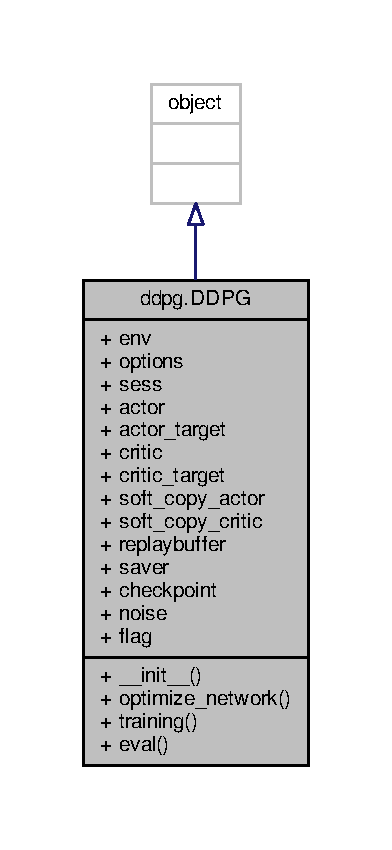
\includegraphics[width=188pt]{classddpg_1_1_d_d_p_g__inherit__graph}
\end{center}
\end{figure}


Sadarbības diagramma klasei ddpg.\+D\+D\+PG\+:
\nopagebreak
\begin{figure}[H]
\begin{center}
\leavevmode
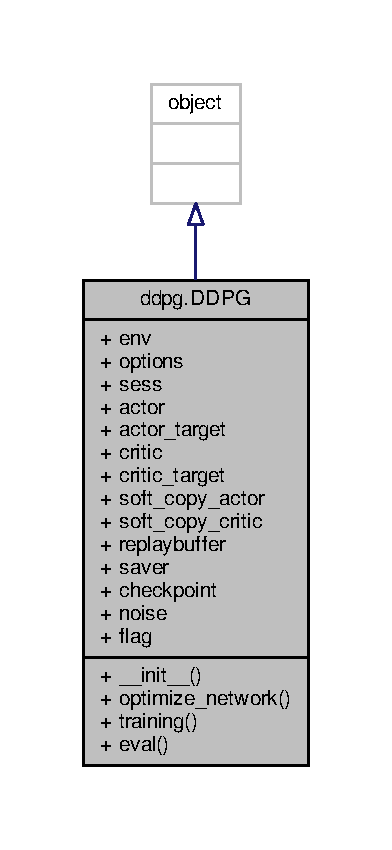
\includegraphics[width=188pt]{classddpg_1_1_d_d_p_g__coll__graph}
\end{center}
\end{figure}
\subsection*{Publiskās elementa funkcijas}
\begin{DoxyCompactItemize}
\item 
def \hyperlink{classddpg_1_1_d_d_p_g_ae5e2615ed363feea9c437913b1cfc71f}{\+\_\+\+\_\+init\+\_\+\+\_\+} (self)
\item 
def \hyperlink{classddpg_1_1_d_d_p_g_a06c8a226bfc7c56f33a74da00ed8bcec}{optimize\+\_\+network} (self)
\item 
def \hyperlink{classddpg_1_1_d_d_p_g_a5237a908e38e5ac76c6b733fc61aeb3d}{training} (self, goal\+\_\+step)
\item 
def \hyperlink{classddpg_1_1_d_d_p_g_a2784ad40da92d5131c80f25736b0413b}{eval} (self)
\end{DoxyCompactItemize}
\subsection*{Publiskie atribūti}
\begin{DoxyCompactItemize}
\item 
\hyperlink{classddpg_1_1_d_d_p_g_a7faf017eedf2120a89e584563d2b80b1}{env}
\item 
\hyperlink{classddpg_1_1_d_d_p_g_a20c64c2cb91fbfa0c705fbab17f027ee}{options}
\item 
\hyperlink{classddpg_1_1_d_d_p_g_a9fed3bda5c1636b1c4bb89fe3a4293c5}{sess}
\item 
\hyperlink{classddpg_1_1_d_d_p_g_ae6f6b492a3680ece32923bb5f145011f}{actor}
\item 
\hyperlink{classddpg_1_1_d_d_p_g_a8b144476a564ad7483fc276939d27f31}{actor\+\_\+target}
\item 
\hyperlink{classddpg_1_1_d_d_p_g_a75e1fa4557d41a8685f47d2d2d730479}{critic}
\item 
\hyperlink{classddpg_1_1_d_d_p_g_a3c8e5f26e9a64fb7af68b7e96d9c8b49}{critic\+\_\+target}
\item 
\hyperlink{classddpg_1_1_d_d_p_g_a2bb041b9ab7c84c83f584a1eae593a87}{soft\+\_\+copy\+\_\+actor}
\item 
\hyperlink{classddpg_1_1_d_d_p_g_a01b575596a4ae50a5ee3656ce9529c94}{soft\+\_\+copy\+\_\+critic}
\item 
\hyperlink{classddpg_1_1_d_d_p_g_af2e26e10a5dd5209afa7a6f3b7d16ab7}{replaybuffer}
\item 
\hyperlink{classddpg_1_1_d_d_p_g_acbd64c92b0d268210807f4e10a214039}{saver}
\item 
\hyperlink{classddpg_1_1_d_d_p_g_a9e0f7ad3975f13452b47eb0a3c5194c7}{checkpoint}
\item 
\hyperlink{classddpg_1_1_d_d_p_g_a9b3d7ee697bd6d7657e0e35b4c1cbd2f}{noise}
\item 
\hyperlink{classddpg_1_1_d_d_p_g_ae456a944d9035ea92e16b3b5d9852dcb}{flag}
\end{DoxyCompactItemize}


\subsection{Detalizēts apraksts}


Definēts līnijā 19 failā ddpg.\+py.



\subsection{Konstruktora un destruktora dokumentācija}
\index{ddpg\+::\+D\+D\+PG@{ddpg\+::\+D\+D\+PG}!\+\_\+\+\_\+init\+\_\+\+\_\+@{\+\_\+\+\_\+init\+\_\+\+\_\+}}
\index{\+\_\+\+\_\+init\+\_\+\+\_\+@{\+\_\+\+\_\+init\+\_\+\+\_\+}!ddpg\+::\+D\+D\+PG@{ddpg\+::\+D\+D\+PG}}
\subsubsection[{\texorpdfstring{\+\_\+\+\_\+init\+\_\+\+\_\+(self)}{__init__(self)}}]{\setlength{\rightskip}{0pt plus 5cm}def ddpg.\+D\+D\+P\+G.\+\_\+\+\_\+init\+\_\+\+\_\+ (
\begin{DoxyParamCaption}
\item[{}]{self}
\end{DoxyParamCaption}
)}\hypertarget{classddpg_1_1_d_d_p_g_ae5e2615ed363feea9c437913b1cfc71f}{}\label{classddpg_1_1_d_d_p_g_ae5e2615ed363feea9c437913b1cfc71f}


Definēts līnijā 20 failā ddpg.\+py.


\begin{DoxyCode}
20     \textcolor{keyword}{def }\hyperlink{classddpg_1_1_d_d_p_g_ae5e2615ed363feea9c437913b1cfc71f}{\_\_init\_\_}(self):
21         self.\hyperlink{classddpg_1_1_d_d_p_g_a7faf017eedf2120a89e584563d2b80b1}{env} = \hyperlink{classenv_1_1_environment}{Environment}()
22         self.\hyperlink{classddpg_1_1_d_d_p_g_a20c64c2cb91fbfa0c705fbab17f027ee}{options} = \hyperlink{classoptions_1_1_options}{Options}().get\_options()
23         self.\hyperlink{classddpg_1_1_d_d_p_g_a9fed3bda5c1636b1c4bb89fe3a4293c5}{sess} = tf.Session()
24 
25         \textcolor{comment}{# actor}
26         self.\hyperlink{classddpg_1_1_d_d_p_g_ae6f6b492a3680ece32923bb5f145011f}{actor} = Actor(self.\hyperlink{classddpg_1_1_d_d_p_g_a9fed3bda5c1636b1c4bb89fe3a4293c5}{sess}, self.\hyperlink{classddpg_1_1_d_d_p_g_a20c64c2cb91fbfa0c705fbab17f027ee}{options}, name=\textcolor{stringliteral}{"actor"})
27         self.\hyperlink{classddpg_1_1_d_d_p_g_a8b144476a564ad7483fc276939d27f31}{actor\_target} = Actor(self.\hyperlink{classddpg_1_1_d_d_p_g_a9fed3bda5c1636b1c4bb89fe3a4293c5}{sess}, self.\hyperlink{classddpg_1_1_d_d_p_g_a20c64c2cb91fbfa0c705fbab17f027ee}{options}, name=\textcolor{stringliteral}{"actor\_target"})
28 
29         \textcolor{comment}{# critic}
30         self.\hyperlink{classddpg_1_1_d_d_p_g_a75e1fa4557d41a8685f47d2d2d730479}{critic} = Critic(self.\hyperlink{classddpg_1_1_d_d_p_g_a9fed3bda5c1636b1c4bb89fe3a4293c5}{sess}, self.\hyperlink{classddpg_1_1_d_d_p_g_a20c64c2cb91fbfa0c705fbab17f027ee}{options}, name=\textcolor{stringliteral}{"critic"})
31         self.\hyperlink{classddpg_1_1_d_d_p_g_a3c8e5f26e9a64fb7af68b7e96d9c8b49}{critic\_target} = Critic(self.\hyperlink{classddpg_1_1_d_d_p_g_a9fed3bda5c1636b1c4bb89fe3a4293c5}{sess}, self.\hyperlink{classddpg_1_1_d_d_p_g_a20c64c2cb91fbfa0c705fbab17f027ee}{options}, name=\textcolor{stringliteral}{"critic\_target"})
32 
33         \textcolor{comment}{# soft copy}
34         self.\hyperlink{classddpg_1_1_d_d_p_g_a2bb041b9ab7c84c83f584a1eae593a87}{soft\_copy\_actor} = \(\backslash\)
35             [self.actor\_target.network\_params[i].assign(
36                 tf.multiply(self.actor.network\_params[i], self.options.TAU) + \(\backslash\)
37                 tf.multiply(self.actor\_target.network\_params[i], 1. - self.options.TAU)) \(\backslash\)
38                 \textcolor{keywordflow}{for} i \textcolor{keywordflow}{in} range(len(self.actor\_target.network\_params)
39             )]
40 
41         self.\hyperlink{classddpg_1_1_d_d_p_g_a01b575596a4ae50a5ee3656ce9529c94}{soft\_copy\_critic} = \(\backslash\)
42             [self.critic\_target.network\_params[i].assign(
43                 tf.multiply(self.critic.network\_params[i], self.options.TAU) + \(\backslash\)
44                 tf.multiply(self.critic\_target.network\_params[i], 1. - self.options.TAU)) \(\backslash\)
45                 \textcolor{keywordflow}{for} i \textcolor{keywordflow}{in} range(len(self.critic\_target.network\_params)
46             )]
47 
48         \textcolor{comment}{# replay buffer}
49         self.\hyperlink{classddpg_1_1_d_d_p_g_af2e26e10a5dd5209afa7a6f3b7d16ab7}{replaybuffer} = \hyperlink{classreplaybuffer_1_1_replay_buffer}{ReplayBuffer}(self.options.BUFFER\_SIZE)
50 
51         \textcolor{comment}{# saving and loading networks}
52         self.\hyperlink{classddpg_1_1_d_d_p_g_acbd64c92b0d268210807f4e10a214039}{saver} = tf.train.Saver()
53         self.\hyperlink{classddpg_1_1_d_d_p_g_a9e0f7ad3975f13452b47eb0a3c5194c7}{checkpoint} = tf.train.get\_checkpoint\_state(\textcolor{stringliteral}{"checkpoints-cartpole"})
54         \textcolor{keywordflow}{if} self.\hyperlink{classddpg_1_1_d_d_p_g_a9e0f7ad3975f13452b47eb0a3c5194c7}{checkpoint} \textcolor{keywordflow}{and} self.checkpoint.model\_checkpoint\_path:
55             self.saver.restore(self.\hyperlink{classddpg_1_1_d_d_p_g_a9fed3bda5c1636b1c4bb89fe3a4293c5}{sess}, self.checkpoint.model\_checkpoint\_path)
56             print(\textcolor{stringliteral}{"Successfully loaded:"}, self.checkpoint.model\_checkpoint\_path)
57         \textcolor{keywordflow}{else}:
58             print(\textcolor{stringliteral}{"Could not find old network weights"})
59 
60         \textcolor{comment}{# gaussian noise}
61         self.\hyperlink{classddpg_1_1_d_d_p_g_a9b3d7ee697bd6d7657e0e35b4c1cbd2f}{noise} = \hyperlink{classnoise_1_1_gaussian_noise}{GaussianNoise}()
62 
63         self.\hyperlink{classddpg_1_1_d_d_p_g_ae456a944d9035ea92e16b3b5d9852dcb}{flag} = \textcolor{keywordtype}{None}
64 
\end{DoxyCode}


\subsection{Elementa funkcijas dokumentācija}
\index{ddpg\+::\+D\+D\+PG@{ddpg\+::\+D\+D\+PG}!eval@{eval}}
\index{eval@{eval}!ddpg\+::\+D\+D\+PG@{ddpg\+::\+D\+D\+PG}}
\subsubsection[{\texorpdfstring{eval(self)}{eval(self)}}]{\setlength{\rightskip}{0pt plus 5cm}def ddpg.\+D\+D\+P\+G.\+eval (
\begin{DoxyParamCaption}
\item[{}]{self}
\end{DoxyParamCaption}
)}\hypertarget{classddpg_1_1_d_d_p_g_a2784ad40da92d5131c80f25736b0413b}{}\label{classddpg_1_1_d_d_p_g_a2784ad40da92d5131c80f25736b0413b}


Definēts līnijā 145 failā ddpg.\+py.


\begin{DoxyCode}
145     \textcolor{keyword}{def }\hyperlink{classddpg_1_1_d_d_p_g_a2784ad40da92d5131c80f25736b0413b}{eval}(self):
146         print(\textcolor{stringliteral}{"Start evaluation"})
147         self.env.reset()
148         state = self.env.getState()
149         done = \textcolor{keyword}{False}
150         total\_reward = 0
151         \textcolor{keywordflow}{while} \textcolor{keywordflow}{not} done \textcolor{keywordflow}{and} total\_reward < self.options.GOAL\_REWARD:
152             action = float(self.actor.predict(state)[0][0])
153 
154             \textcolor{comment}{# stepping}
155             self.env.setAction(action)
156             self.env.step(\textcolor{keyword}{True})
157             reward = self.env.getReward()
158             next\_state = self.env.getState()
159             done = self.env.getDone()
160             state = next\_state
161             total\_reward += reward
162 
163         \textcolor{keywordflow}{print} \textcolor{stringliteral}{'eval: '}, total\_reward\end{DoxyCode}
\index{ddpg\+::\+D\+D\+PG@{ddpg\+::\+D\+D\+PG}!optimize\+\_\+network@{optimize\+\_\+network}}
\index{optimize\+\_\+network@{optimize\+\_\+network}!ddpg\+::\+D\+D\+PG@{ddpg\+::\+D\+D\+PG}}
\subsubsection[{\texorpdfstring{optimize\+\_\+network(self)}{optimize_network(self)}}]{\setlength{\rightskip}{0pt plus 5cm}def ddpg.\+D\+D\+P\+G.\+optimize\+\_\+network (
\begin{DoxyParamCaption}
\item[{}]{self}
\end{DoxyParamCaption}
)}\hypertarget{classddpg_1_1_d_d_p_g_a06c8a226bfc7c56f33a74da00ed8bcec}{}\label{classddpg_1_1_d_d_p_g_a06c8a226bfc7c56f33a74da00ed8bcec}


Definēts līnijā 65 failā ddpg.\+py.


\begin{DoxyCode}
65     \textcolor{keyword}{def }\hyperlink{classddpg_1_1_d_d_p_g_a06c8a226bfc7c56f33a74da00ed8bcec}{optimize\_network}(self):
66         \textcolor{keywordflow}{if} self.replaybuffer.size() < self.options.BUFFER\_SIZE:
67             \textcolor{keywordflow}{return}
68         \textcolor{keywordflow}{if} self.\hyperlink{classddpg_1_1_d_d_p_g_ae456a944d9035ea92e16b3b5d9852dcb}{flag} == \textcolor{keywordtype}{None}:
69             self.\hyperlink{classddpg_1_1_d_d_p_g_ae456a944d9035ea92e16b3b5d9852dcb}{flag} = \textcolor{keyword}{True}
70             \textcolor{keywordflow}{print} \textcolor{stringliteral}{'OPT'}
71         s\_batch, a\_batch, r\_batch, s2\_batch = self.replaybuffer.sample\_batch(self.options.BATCH\_SIZE)
72 
73         action\_target\_batch = self.actor\_target.predict(s2\_batch)
74         q\_target\_batch = r\_batch + self.options.GAMMA * self.critic\_target.predict(s2\_batch, 
      action\_target\_batch)
75         self.critic.update(s\_batch, a\_batch, q\_target\_batch)
76 
77         action\_train\_batch = self.actor.predict(s\_batch)
78         q\_grad\_batch = self.critic.compute\_grad(s\_batch, action\_train\_batch)
79         \textcolor{comment}{# idxs=[]}
80         \textcolor{comment}{# for i in range(len(q\_grad\_batch)):}
81         \textcolor{comment}{#   if (q\_grad\_batch[i] < 0):}
82         \textcolor{comment}{#       idxs.append(i)}
83         \textcolor{comment}{# s\_batch = s\_batch[idxs]}
84         \textcolor{comment}{# q\_grad\_batch = q\_grad\_batch[idxs]}
85 
86         self.actor.update(s\_batch, q\_grad\_batch)
87 
88         self.sess.run(self.\hyperlink{classddpg_1_1_d_d_p_g_a2bb041b9ab7c84c83f584a1eae593a87}{soft\_copy\_actor})  
89         self.sess.run(self.\hyperlink{classddpg_1_1_d_d_p_g_a01b575596a4ae50a5ee3656ce9529c94}{soft\_copy\_critic})    
90 
\end{DoxyCode}


Šeit ir šīs funkcijas izsaukuma grafs\+:
\nopagebreak
\begin{figure}[H]
\begin{center}
\leavevmode
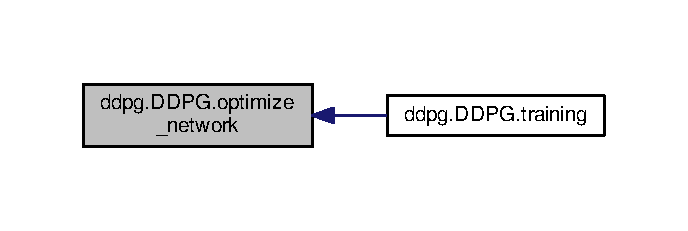
\includegraphics[width=330pt]{classddpg_1_1_d_d_p_g_a06c8a226bfc7c56f33a74da00ed8bcec_icgraph}
\end{center}
\end{figure}


\index{ddpg\+::\+D\+D\+PG@{ddpg\+::\+D\+D\+PG}!training@{training}}
\index{training@{training}!ddpg\+::\+D\+D\+PG@{ddpg\+::\+D\+D\+PG}}
\subsubsection[{\texorpdfstring{training(self, goal\+\_\+step)}{training(self, goal_step)}}]{\setlength{\rightskip}{0pt plus 5cm}def ddpg.\+D\+D\+P\+G.\+training (
\begin{DoxyParamCaption}
\item[{}]{self, }
\item[{}]{goal\+\_\+step}
\end{DoxyParamCaption}
)}\hypertarget{classddpg_1_1_d_d_p_g_a5237a908e38e5ac76c6b733fc61aeb3d}{}\label{classddpg_1_1_d_d_p_g_a5237a908e38e5ac76c6b733fc61aeb3d}


Definēts līnijā 91 failā ddpg.\+py.


\begin{DoxyCode}
91     \textcolor{keyword}{def }\hyperlink{classddpg_1_1_d_d_p_g_a5237a908e38e5ac76c6b733fc61aeb3d}{training}(self, goal\_step):
92         print(\textcolor{stringliteral}{"Start training"})
93         global\_step = 0
94         eps = self.options.INIT\_EPS
95         mem = \textcolor{keyword}{False}
96         \textcolor{keywordflow}{for} t \textcolor{keywordflow}{in} range(self.options.MAX\_EPISODE):
97             local\_step = 0
98             done = \textcolor{keyword}{False}
99             self.env.reset()
100             state = self.env.getState()
101             total\_reward = 0
102 
103             \textcolor{keywordflow}{while} local\_step < goal\_step:
104                 \textcolor{comment}{# epsilon decaying}
105                 global\_step += 1
106                 local\_step += 1
107                 \textcolor{keywordflow}{if} global\_step % self.options.EPS\_ANNEAL\_STEPS == 0 \textcolor{keywordflow}{and} eps > self.options.FINAL\_EPS:
108                     eps = eps * self.options.EPS\_DECAY
109 
110                 \textcolor{comment}{# # epsilon exploration}
111                 \textcolor{comment}{# if np.random.uniform(0,1) < eps:}
112                 \textcolor{comment}{#   action = np.random.normal(float(self.actor.predict(state)[0][0]), 0.3) # sigma = 0.3}
113                 \textcolor{comment}{# else:}
114                 \textcolor{comment}{#   action = float(self.actor.predict(state)[0][0])}
115                 
116                 print(actor.predict(state)[0][0])
117                 \textcolor{comment}{# action = np.random.normal(float(self.actor.predict(state)[0][0]), eps) # sigma = 0.3}
118                 \textcolor{comment}{#action = normlNoise(action, eps)}
119 
120 
121                 \textcolor{comment}{# stepping}
122                 self.env.setAction(action)
123                 self.env.step(\textcolor{keyword}{True})
124                 reward = self.env.getReward()
125                 next\_state = self.env.getState()
126                 done = self.env.getDone()
127                 \textcolor{comment}{# if done and total\_reward < self.options.GOAL\_REWARD:}
128                 \textcolor{comment}{#   reward = -1000}
129 
130                 \textcolor{comment}{# training}
131                 self.replaybuffer.add(state, [action], [reward], next\_state)
132                 self.\hyperlink{classddpg_1_1_d_d_p_g_a06c8a226bfc7c56f33a74da00ed8bcec}{optimize\_network}()
133 
134                 state = next\_state
135                 total\_reward += reward
136 
137             \textcolor{keywordflow}{if} total\_reward == self.options.GOAL\_REWARD:
138                 mem = \textcolor{keyword}{True}
139             \textcolor{keywordflow}{else}:
140                 mem = \textcolor{keyword}{False}
141             \textcolor{keywordflow}{if} (t+1)%500==0:
142                 self.saver.save(self.\hyperlink{classddpg_1_1_d_d_p_g_a9fed3bda5c1636b1c4bb89fe3a4293c5}{sess}, \textcolor{stringliteral}{'checkpoints-simbicon/simbicon\_ddpg'}, global\_step = 
      global\_step)
143             print(t, total\_reward)
144 
\end{DoxyCode}


Šeit ir visu funkciju izsaugumu grafs\+:
\nopagebreak
\begin{figure}[H]
\begin{center}
\leavevmode
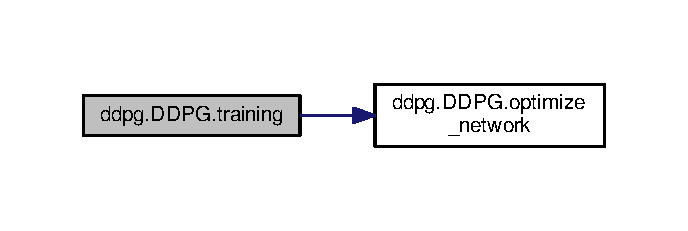
\includegraphics[width=330pt]{classddpg_1_1_d_d_p_g_a5237a908e38e5ac76c6b733fc61aeb3d_cgraph}
\end{center}
\end{figure}




\subsection{Elementa datu dokumentācija}
\index{ddpg\+::\+D\+D\+PG@{ddpg\+::\+D\+D\+PG}!actor@{actor}}
\index{actor@{actor}!ddpg\+::\+D\+D\+PG@{ddpg\+::\+D\+D\+PG}}
\subsubsection[{\texorpdfstring{actor}{actor}}]{\setlength{\rightskip}{0pt plus 5cm}ddpg.\+D\+D\+P\+G.\+actor}\hypertarget{classddpg_1_1_d_d_p_g_ae6f6b492a3680ece32923bb5f145011f}{}\label{classddpg_1_1_d_d_p_g_ae6f6b492a3680ece32923bb5f145011f}


Definēts līnijā 26 failā ddpg.\+py.

\index{ddpg\+::\+D\+D\+PG@{ddpg\+::\+D\+D\+PG}!actor\+\_\+target@{actor\+\_\+target}}
\index{actor\+\_\+target@{actor\+\_\+target}!ddpg\+::\+D\+D\+PG@{ddpg\+::\+D\+D\+PG}}
\subsubsection[{\texorpdfstring{actor\+\_\+target}{actor_target}}]{\setlength{\rightskip}{0pt plus 5cm}ddpg.\+D\+D\+P\+G.\+actor\+\_\+target}\hypertarget{classddpg_1_1_d_d_p_g_a8b144476a564ad7483fc276939d27f31}{}\label{classddpg_1_1_d_d_p_g_a8b144476a564ad7483fc276939d27f31}


Definēts līnijā 27 failā ddpg.\+py.

\index{ddpg\+::\+D\+D\+PG@{ddpg\+::\+D\+D\+PG}!checkpoint@{checkpoint}}
\index{checkpoint@{checkpoint}!ddpg\+::\+D\+D\+PG@{ddpg\+::\+D\+D\+PG}}
\subsubsection[{\texorpdfstring{checkpoint}{checkpoint}}]{\setlength{\rightskip}{0pt plus 5cm}ddpg.\+D\+D\+P\+G.\+checkpoint}\hypertarget{classddpg_1_1_d_d_p_g_a9e0f7ad3975f13452b47eb0a3c5194c7}{}\label{classddpg_1_1_d_d_p_g_a9e0f7ad3975f13452b47eb0a3c5194c7}


Definēts līnijā 53 failā ddpg.\+py.

\index{ddpg\+::\+D\+D\+PG@{ddpg\+::\+D\+D\+PG}!critic@{critic}}
\index{critic@{critic}!ddpg\+::\+D\+D\+PG@{ddpg\+::\+D\+D\+PG}}
\subsubsection[{\texorpdfstring{critic}{critic}}]{\setlength{\rightskip}{0pt plus 5cm}ddpg.\+D\+D\+P\+G.\+critic}\hypertarget{classddpg_1_1_d_d_p_g_a75e1fa4557d41a8685f47d2d2d730479}{}\label{classddpg_1_1_d_d_p_g_a75e1fa4557d41a8685f47d2d2d730479}


Definēts līnijā 30 failā ddpg.\+py.

\index{ddpg\+::\+D\+D\+PG@{ddpg\+::\+D\+D\+PG}!critic\+\_\+target@{critic\+\_\+target}}
\index{critic\+\_\+target@{critic\+\_\+target}!ddpg\+::\+D\+D\+PG@{ddpg\+::\+D\+D\+PG}}
\subsubsection[{\texorpdfstring{critic\+\_\+target}{critic_target}}]{\setlength{\rightskip}{0pt plus 5cm}ddpg.\+D\+D\+P\+G.\+critic\+\_\+target}\hypertarget{classddpg_1_1_d_d_p_g_a3c8e5f26e9a64fb7af68b7e96d9c8b49}{}\label{classddpg_1_1_d_d_p_g_a3c8e5f26e9a64fb7af68b7e96d9c8b49}


Definēts līnijā 31 failā ddpg.\+py.

\index{ddpg\+::\+D\+D\+PG@{ddpg\+::\+D\+D\+PG}!env@{env}}
\index{env@{env}!ddpg\+::\+D\+D\+PG@{ddpg\+::\+D\+D\+PG}}
\subsubsection[{\texorpdfstring{env}{env}}]{\setlength{\rightskip}{0pt plus 5cm}ddpg.\+D\+D\+P\+G.\+env}\hypertarget{classddpg_1_1_d_d_p_g_a7faf017eedf2120a89e584563d2b80b1}{}\label{classddpg_1_1_d_d_p_g_a7faf017eedf2120a89e584563d2b80b1}


Definēts līnijā 21 failā ddpg.\+py.

\index{ddpg\+::\+D\+D\+PG@{ddpg\+::\+D\+D\+PG}!flag@{flag}}
\index{flag@{flag}!ddpg\+::\+D\+D\+PG@{ddpg\+::\+D\+D\+PG}}
\subsubsection[{\texorpdfstring{flag}{flag}}]{\setlength{\rightskip}{0pt plus 5cm}ddpg.\+D\+D\+P\+G.\+flag}\hypertarget{classddpg_1_1_d_d_p_g_ae456a944d9035ea92e16b3b5d9852dcb}{}\label{classddpg_1_1_d_d_p_g_ae456a944d9035ea92e16b3b5d9852dcb}


Definēts līnijā 63 failā ddpg.\+py.

\index{ddpg\+::\+D\+D\+PG@{ddpg\+::\+D\+D\+PG}!noise@{noise}}
\index{noise@{noise}!ddpg\+::\+D\+D\+PG@{ddpg\+::\+D\+D\+PG}}
\subsubsection[{\texorpdfstring{noise}{noise}}]{\setlength{\rightskip}{0pt plus 5cm}ddpg.\+D\+D\+P\+G.\+noise}\hypertarget{classddpg_1_1_d_d_p_g_a9b3d7ee697bd6d7657e0e35b4c1cbd2f}{}\label{classddpg_1_1_d_d_p_g_a9b3d7ee697bd6d7657e0e35b4c1cbd2f}


Definēts līnijā 61 failā ddpg.\+py.

\index{ddpg\+::\+D\+D\+PG@{ddpg\+::\+D\+D\+PG}!options@{options}}
\index{options@{options}!ddpg\+::\+D\+D\+PG@{ddpg\+::\+D\+D\+PG}}
\subsubsection[{\texorpdfstring{options}{options}}]{\setlength{\rightskip}{0pt plus 5cm}ddpg.\+D\+D\+P\+G.\+options}\hypertarget{classddpg_1_1_d_d_p_g_a20c64c2cb91fbfa0c705fbab17f027ee}{}\label{classddpg_1_1_d_d_p_g_a20c64c2cb91fbfa0c705fbab17f027ee}


Definēts līnijā 22 failā ddpg.\+py.

\index{ddpg\+::\+D\+D\+PG@{ddpg\+::\+D\+D\+PG}!replaybuffer@{replaybuffer}}
\index{replaybuffer@{replaybuffer}!ddpg\+::\+D\+D\+PG@{ddpg\+::\+D\+D\+PG}}
\subsubsection[{\texorpdfstring{replaybuffer}{replaybuffer}}]{\setlength{\rightskip}{0pt plus 5cm}ddpg.\+D\+D\+P\+G.\+replaybuffer}\hypertarget{classddpg_1_1_d_d_p_g_af2e26e10a5dd5209afa7a6f3b7d16ab7}{}\label{classddpg_1_1_d_d_p_g_af2e26e10a5dd5209afa7a6f3b7d16ab7}


Definēts līnijā 49 failā ddpg.\+py.

\index{ddpg\+::\+D\+D\+PG@{ddpg\+::\+D\+D\+PG}!saver@{saver}}
\index{saver@{saver}!ddpg\+::\+D\+D\+PG@{ddpg\+::\+D\+D\+PG}}
\subsubsection[{\texorpdfstring{saver}{saver}}]{\setlength{\rightskip}{0pt plus 5cm}ddpg.\+D\+D\+P\+G.\+saver}\hypertarget{classddpg_1_1_d_d_p_g_acbd64c92b0d268210807f4e10a214039}{}\label{classddpg_1_1_d_d_p_g_acbd64c92b0d268210807f4e10a214039}


Definēts līnijā 52 failā ddpg.\+py.

\index{ddpg\+::\+D\+D\+PG@{ddpg\+::\+D\+D\+PG}!sess@{sess}}
\index{sess@{sess}!ddpg\+::\+D\+D\+PG@{ddpg\+::\+D\+D\+PG}}
\subsubsection[{\texorpdfstring{sess}{sess}}]{\setlength{\rightskip}{0pt plus 5cm}ddpg.\+D\+D\+P\+G.\+sess}\hypertarget{classddpg_1_1_d_d_p_g_a9fed3bda5c1636b1c4bb89fe3a4293c5}{}\label{classddpg_1_1_d_d_p_g_a9fed3bda5c1636b1c4bb89fe3a4293c5}


Definēts līnijā 23 failā ddpg.\+py.

\index{ddpg\+::\+D\+D\+PG@{ddpg\+::\+D\+D\+PG}!soft\+\_\+copy\+\_\+actor@{soft\+\_\+copy\+\_\+actor}}
\index{soft\+\_\+copy\+\_\+actor@{soft\+\_\+copy\+\_\+actor}!ddpg\+::\+D\+D\+PG@{ddpg\+::\+D\+D\+PG}}
\subsubsection[{\texorpdfstring{soft\+\_\+copy\+\_\+actor}{soft_copy_actor}}]{\setlength{\rightskip}{0pt plus 5cm}ddpg.\+D\+D\+P\+G.\+soft\+\_\+copy\+\_\+actor}\hypertarget{classddpg_1_1_d_d_p_g_a2bb041b9ab7c84c83f584a1eae593a87}{}\label{classddpg_1_1_d_d_p_g_a2bb041b9ab7c84c83f584a1eae593a87}


Definēts līnijā 34 failā ddpg.\+py.

\index{ddpg\+::\+D\+D\+PG@{ddpg\+::\+D\+D\+PG}!soft\+\_\+copy\+\_\+critic@{soft\+\_\+copy\+\_\+critic}}
\index{soft\+\_\+copy\+\_\+critic@{soft\+\_\+copy\+\_\+critic}!ddpg\+::\+D\+D\+PG@{ddpg\+::\+D\+D\+PG}}
\subsubsection[{\texorpdfstring{soft\+\_\+copy\+\_\+critic}{soft_copy_critic}}]{\setlength{\rightskip}{0pt plus 5cm}ddpg.\+D\+D\+P\+G.\+soft\+\_\+copy\+\_\+critic}\hypertarget{classddpg_1_1_d_d_p_g_a01b575596a4ae50a5ee3656ce9529c94}{}\label{classddpg_1_1_d_d_p_g_a01b575596a4ae50a5ee3656ce9529c94}


Definēts līnijā 41 failā ddpg.\+py.



Šīs klases dokumentācijas tika ģenerēta no šāda faila\+:\begin{DoxyCompactItemize}
\item 
py\+\_\+code/\hyperlink{ddpg_8py}{ddpg.\+py}\end{DoxyCompactItemize}

\hypertarget{classenv_1_1_environment}{}\section{env.\+Environment klases apraksts}
\label{classenv_1_1_environment}\index{env.\+Environment@{env.\+Environment}}


Sadarbības diagramma klasei env.\+Environment\+:
\nopagebreak
\begin{figure}[H]
\begin{center}
\leavevmode
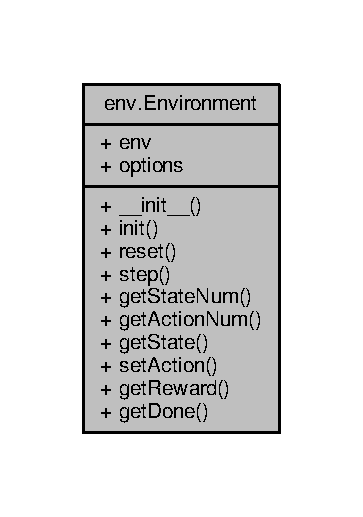
\includegraphics[width=174pt]{classenv_1_1_environment__coll__graph}
\end{center}
\end{figure}
\subsection*{Publiskās elementa funkcijas}
\begin{DoxyCompactItemize}
\item 
def \hyperlink{classenv_1_1_environment_ab43aa325dc7ec51e135ea24d2e6d8954}{\+\_\+\+\_\+init\+\_\+\+\_\+} (self)
\item 
def \hyperlink{classenv_1_1_environment_a8dd860a9d167e765134f08344a2c2d71}{init} (self)
\item 
def \hyperlink{classenv_1_1_environment_a33c77a544170cb422c7bcc6e257e9e66}{reset} (self)
\item 
def \hyperlink{classenv_1_1_environment_afb163b7692002933d860d3bd00a9e869}{step} (self, flag)
\item 
def \hyperlink{classenv_1_1_environment_a03b485c5cd7d6a33b0563fb074989b5f}{get\+State\+Num} (self)
\item 
def \hyperlink{classenv_1_1_environment_a33704b8916e5dbca53031fa89dd5ccb0}{get\+Action\+Num} (self)
\item 
def \hyperlink{classenv_1_1_environment_adbbb2aecb72314a5337fece8e433fe35}{get\+State} (self)
\item 
def \hyperlink{classenv_1_1_environment_a9cc0fbe9f5e1fbe3c49a3fb412d591d1}{set\+Action} (self, action)
\item 
def \hyperlink{classenv_1_1_environment_a3ed8a37b7b6c1279a10af783352335a6}{get\+Reward} (self)
\item 
def \hyperlink{classenv_1_1_environment_aa44deb3deae93e541af1d23523e28969}{get\+Done} (self)
\end{DoxyCompactItemize}
\subsection*{Publiskie atribūti}
\begin{DoxyCompactItemize}
\item 
\hyperlink{classenv_1_1_environment_ae1915ac7b5e3da938948b6f6f57a3dfa}{env}
\item 
\hyperlink{classenv_1_1_environment_a60104200654a882002d5be49bb6843de}{options}
\end{DoxyCompactItemize}


\subsection{Detalizēts apraksts}


Definēts līnijā 4 failā env.\+py.



\subsection{Konstruktora un destruktora dokumentācija}
\index{env\+::\+Environment@{env\+::\+Environment}!\+\_\+\+\_\+init\+\_\+\+\_\+@{\+\_\+\+\_\+init\+\_\+\+\_\+}}
\index{\+\_\+\+\_\+init\+\_\+\+\_\+@{\+\_\+\+\_\+init\+\_\+\+\_\+}!env\+::\+Environment@{env\+::\+Environment}}
\subsubsection[{\texorpdfstring{\+\_\+\+\_\+init\+\_\+\+\_\+(self)}{__init__(self)}}]{\setlength{\rightskip}{0pt plus 5cm}def env.\+Environment.\+\_\+\+\_\+init\+\_\+\+\_\+ (
\begin{DoxyParamCaption}
\item[{}]{self}
\end{DoxyParamCaption}
)}\hypertarget{classenv_1_1_environment_ab43aa325dc7ec51e135ea24d2e6d8954}{}\label{classenv_1_1_environment_ab43aa325dc7ec51e135ea24d2e6d8954}


Definēts līnijā 5 failā env.\+py.


\begin{DoxyCode}
5     \textcolor{keyword}{def }\hyperlink{classenv_1_1_environment_ab43aa325dc7ec51e135ea24d2e6d8954}{\_\_init\_\_}(self):
6         self.\hyperlink{classenv_1_1_environment_ae1915ac7b5e3da938948b6f6f57a3dfa}{env} = cp.Simulation()
7         self.env.init()
8         self.\hyperlink{classenv_1_1_environment_a60104200654a882002d5be49bb6843de}{options} = \hyperlink{classoptions_1_1_options}{Options}().get\_options()
9 
\end{DoxyCode}


\subsection{Elementa funkcijas dokumentācija}
\index{env\+::\+Environment@{env\+::\+Environment}!get\+Action\+Num@{get\+Action\+Num}}
\index{get\+Action\+Num@{get\+Action\+Num}!env\+::\+Environment@{env\+::\+Environment}}
\subsubsection[{\texorpdfstring{get\+Action\+Num(self)}{getActionNum(self)}}]{\setlength{\rightskip}{0pt plus 5cm}def env.\+Environment.\+get\+Action\+Num (
\begin{DoxyParamCaption}
\item[{}]{self}
\end{DoxyParamCaption}
)}\hypertarget{classenv_1_1_environment_a33704b8916e5dbca53031fa89dd5ccb0}{}\label{classenv_1_1_environment_a33704b8916e5dbca53031fa89dd5ccb0}


Definēts līnijā 22 failā env.\+py.


\begin{DoxyCode}
22     \textcolor{keyword}{def }\hyperlink{classenv_1_1_environment_a33704b8916e5dbca53031fa89dd5ccb0}{getActionNum}(self):
23         \textcolor{keywordflow}{return} self.env.getActionNum()
24 
\end{DoxyCode}
\index{env\+::\+Environment@{env\+::\+Environment}!get\+Done@{get\+Done}}
\index{get\+Done@{get\+Done}!env\+::\+Environment@{env\+::\+Environment}}
\subsubsection[{\texorpdfstring{get\+Done(self)}{getDone(self)}}]{\setlength{\rightskip}{0pt plus 5cm}def env.\+Environment.\+get\+Done (
\begin{DoxyParamCaption}
\item[{}]{self}
\end{DoxyParamCaption}
)}\hypertarget{classenv_1_1_environment_aa44deb3deae93e541af1d23523e28969}{}\label{classenv_1_1_environment_aa44deb3deae93e541af1d23523e28969}


Definēts līnijā 34 failā env.\+py.


\begin{DoxyCode}
34     \textcolor{keyword}{def }\hyperlink{classenv_1_1_environment_aa44deb3deae93e541af1d23523e28969}{getDone}(self):
35         \textcolor{keywordflow}{return} self.env.getDone()
36 \end{DoxyCode}
\index{env\+::\+Environment@{env\+::\+Environment}!get\+Reward@{get\+Reward}}
\index{get\+Reward@{get\+Reward}!env\+::\+Environment@{env\+::\+Environment}}
\subsubsection[{\texorpdfstring{get\+Reward(self)}{getReward(self)}}]{\setlength{\rightskip}{0pt plus 5cm}def env.\+Environment.\+get\+Reward (
\begin{DoxyParamCaption}
\item[{}]{self}
\end{DoxyParamCaption}
)}\hypertarget{classenv_1_1_environment_a3ed8a37b7b6c1279a10af783352335a6}{}\label{classenv_1_1_environment_a3ed8a37b7b6c1279a10af783352335a6}


Definēts līnijā 31 failā env.\+py.


\begin{DoxyCode}
31     \textcolor{keyword}{def }\hyperlink{classenv_1_1_environment_a3ed8a37b7b6c1279a10af783352335a6}{getReward}(self):
32         \textcolor{keywordflow}{return} self.env.getReward()
33 
\end{DoxyCode}
\index{env\+::\+Environment@{env\+::\+Environment}!get\+State@{get\+State}}
\index{get\+State@{get\+State}!env\+::\+Environment@{env\+::\+Environment}}
\subsubsection[{\texorpdfstring{get\+State(self)}{getState(self)}}]{\setlength{\rightskip}{0pt plus 5cm}def env.\+Environment.\+get\+State (
\begin{DoxyParamCaption}
\item[{}]{self}
\end{DoxyParamCaption}
)}\hypertarget{classenv_1_1_environment_adbbb2aecb72314a5337fece8e433fe35}{}\label{classenv_1_1_environment_adbbb2aecb72314a5337fece8e433fe35}


Definēts līnijā 25 failā env.\+py.


\begin{DoxyCode}
25     \textcolor{keyword}{def }\hyperlink{classenv_1_1_environment_adbbb2aecb72314a5337fece8e433fe35}{getState}(self):
26         \textcolor{keywordflow}{return} self.env.getState()
27 
\end{DoxyCode}
\index{env\+::\+Environment@{env\+::\+Environment}!get\+State\+Num@{get\+State\+Num}}
\index{get\+State\+Num@{get\+State\+Num}!env\+::\+Environment@{env\+::\+Environment}}
\subsubsection[{\texorpdfstring{get\+State\+Num(self)}{getStateNum(self)}}]{\setlength{\rightskip}{0pt plus 5cm}def env.\+Environment.\+get\+State\+Num (
\begin{DoxyParamCaption}
\item[{}]{self}
\end{DoxyParamCaption}
)}\hypertarget{classenv_1_1_environment_a03b485c5cd7d6a33b0563fb074989b5f}{}\label{classenv_1_1_environment_a03b485c5cd7d6a33b0563fb074989b5f}


Definēts līnijā 19 failā env.\+py.


\begin{DoxyCode}
19     \textcolor{keyword}{def }\hyperlink{classenv_1_1_environment_a03b485c5cd7d6a33b0563fb074989b5f}{getStateNum}(self):
20         \textcolor{keywordflow}{return} self.env.getStateNum()
21 
\end{DoxyCode}
\index{env\+::\+Environment@{env\+::\+Environment}!init@{init}}
\index{init@{init}!env\+::\+Environment@{env\+::\+Environment}}
\subsubsection[{\texorpdfstring{init(self)}{init(self)}}]{\setlength{\rightskip}{0pt plus 5cm}def env.\+Environment.\+init (
\begin{DoxyParamCaption}
\item[{}]{self}
\end{DoxyParamCaption}
)}\hypertarget{classenv_1_1_environment_a8dd860a9d167e765134f08344a2c2d71}{}\label{classenv_1_1_environment_a8dd860a9d167e765134f08344a2c2d71}


Definēts līnijā 10 failā env.\+py.


\begin{DoxyCode}
10     \textcolor{keyword}{def }\hyperlink{classenv_1_1_environment_a8dd860a9d167e765134f08344a2c2d71}{init}(self):
11         self.env.init()
12 
\end{DoxyCode}
\index{env\+::\+Environment@{env\+::\+Environment}!reset@{reset}}
\index{reset@{reset}!env\+::\+Environment@{env\+::\+Environment}}
\subsubsection[{\texorpdfstring{reset(self)}{reset(self)}}]{\setlength{\rightskip}{0pt plus 5cm}def env.\+Environment.\+reset (
\begin{DoxyParamCaption}
\item[{}]{self}
\end{DoxyParamCaption}
)}\hypertarget{classenv_1_1_environment_a33c77a544170cb422c7bcc6e257e9e66}{}\label{classenv_1_1_environment_a33c77a544170cb422c7bcc6e257e9e66}


Definēts līnijā 13 failā env.\+py.


\begin{DoxyCode}
13     \textcolor{keyword}{def }\hyperlink{classenv_1_1_environment_a33c77a544170cb422c7bcc6e257e9e66}{reset}(self):
14         self.env.reset()
15 
\end{DoxyCode}
\index{env\+::\+Environment@{env\+::\+Environment}!set\+Action@{set\+Action}}
\index{set\+Action@{set\+Action}!env\+::\+Environment@{env\+::\+Environment}}
\subsubsection[{\texorpdfstring{set\+Action(self, action)}{setAction(self, action)}}]{\setlength{\rightskip}{0pt plus 5cm}def env.\+Environment.\+set\+Action (
\begin{DoxyParamCaption}
\item[{}]{self, }
\item[{}]{action}
\end{DoxyParamCaption}
)}\hypertarget{classenv_1_1_environment_a9cc0fbe9f5e1fbe3c49a3fb412d591d1}{}\label{classenv_1_1_environment_a9cc0fbe9f5e1fbe3c49a3fb412d591d1}


Definēts līnijā 28 failā env.\+py.


\begin{DoxyCode}
28     \textcolor{keyword}{def }\hyperlink{classenv_1_1_environment_a9cc0fbe9f5e1fbe3c49a3fb412d591d1}{setAction}(self, action):
29         \textcolor{keywordflow}{return} self.env.setAction(action)
30 
\end{DoxyCode}
\index{env\+::\+Environment@{env\+::\+Environment}!step@{step}}
\index{step@{step}!env\+::\+Environment@{env\+::\+Environment}}
\subsubsection[{\texorpdfstring{step(self, flag)}{step(self, flag)}}]{\setlength{\rightskip}{0pt plus 5cm}def env.\+Environment.\+step (
\begin{DoxyParamCaption}
\item[{}]{self, }
\item[{}]{flag}
\end{DoxyParamCaption}
)}\hypertarget{classenv_1_1_environment_afb163b7692002933d860d3bd00a9e869}{}\label{classenv_1_1_environment_afb163b7692002933d860d3bd00a9e869}


Definēts līnijā 16 failā env.\+py.


\begin{DoxyCode}
16     \textcolor{keyword}{def }\hyperlink{classenv_1_1_environment_afb163b7692002933d860d3bd00a9e869}{step}(self, flag):
17         self.env.step(flag)
18 
\end{DoxyCode}


\subsection{Elementa datu dokumentācija}
\index{env\+::\+Environment@{env\+::\+Environment}!env@{env}}
\index{env@{env}!env\+::\+Environment@{env\+::\+Environment}}
\subsubsection[{\texorpdfstring{env}{env}}]{\setlength{\rightskip}{0pt plus 5cm}env.\+Environment.\+env}\hypertarget{classenv_1_1_environment_ae1915ac7b5e3da938948b6f6f57a3dfa}{}\label{classenv_1_1_environment_ae1915ac7b5e3da938948b6f6f57a3dfa}


Definēts līnijā 6 failā env.\+py.

\index{env\+::\+Environment@{env\+::\+Environment}!options@{options}}
\index{options@{options}!env\+::\+Environment@{env\+::\+Environment}}
\subsubsection[{\texorpdfstring{options}{options}}]{\setlength{\rightskip}{0pt plus 5cm}env.\+Environment.\+options}\hypertarget{classenv_1_1_environment_a60104200654a882002d5be49bb6843de}{}\label{classenv_1_1_environment_a60104200654a882002d5be49bb6843de}


Definēts līnijā 8 failā env.\+py.



Šīs klases dokumentācijas tika ģenerēta no šāda faila\+:\begin{DoxyCompactItemize}
\item 
py\+\_\+code/\hyperlink{env_8py}{env.\+py}\end{DoxyCompactItemize}

\hypertarget{classnoise_1_1_gaussian_noise}{}\section{noise.\+Gaussian\+Noise klases apraksts}
\label{classnoise_1_1_gaussian_noise}\index{noise.\+Gaussian\+Noise@{noise.\+Gaussian\+Noise}}


Mantojamības diagramma klasei noise.\+Gaussian\+Noise\+:
\nopagebreak
\begin{figure}[H]
\begin{center}
\leavevmode
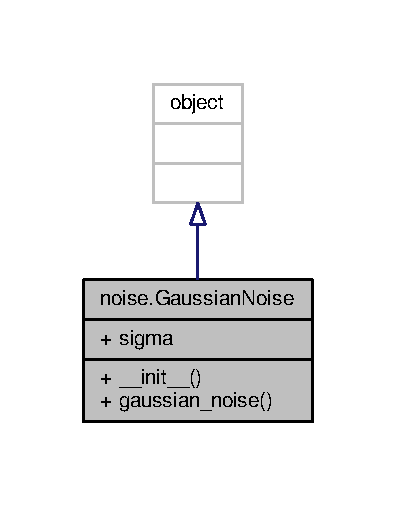
\includegraphics[width=190pt]{classnoise_1_1_gaussian_noise__inherit__graph}
\end{center}
\end{figure}


Sadarbības diagramma klasei noise.\+Gaussian\+Noise\+:
\nopagebreak
\begin{figure}[H]
\begin{center}
\leavevmode
\includegraphics[width=190pt]{classnoise_1_1_gaussian_noise__coll__graph}
\end{center}
\end{figure}
\subsection*{Publiskās elementa funkcijas}
\begin{DoxyCompactItemize}
\item 
def \hyperlink{classnoise_1_1_gaussian_noise_afbab5255dc75d7f01173a2c3231a5083}{\+\_\+\+\_\+init\+\_\+\+\_\+} (self)
\item 
def \hyperlink{classnoise_1_1_gaussian_noise_aa5a9d46ef04a4eef8dfc25e966c0f622}{gaussian\+\_\+noise} (self, mu, \hyperlink{classnoise_1_1_gaussian_noise_ae6ebe290c02cbbddebafa335ef0af013}{sigma}=0.\+3)
\end{DoxyCompactItemize}
\subsection*{Publiskie atribūti}
\begin{DoxyCompactItemize}
\item 
\hyperlink{classnoise_1_1_gaussian_noise_ae6ebe290c02cbbddebafa335ef0af013}{sigma}
\end{DoxyCompactItemize}


\subsection{Detalizēts apraksts}


Definēts līnijā 35 failā noise.\+py.



\subsection{Konstruktora un destruktora dokumentācija}
\index{noise\+::\+Gaussian\+Noise@{noise\+::\+Gaussian\+Noise}!\+\_\+\+\_\+init\+\_\+\+\_\+@{\+\_\+\+\_\+init\+\_\+\+\_\+}}
\index{\+\_\+\+\_\+init\+\_\+\+\_\+@{\+\_\+\+\_\+init\+\_\+\+\_\+}!noise\+::\+Gaussian\+Noise@{noise\+::\+Gaussian\+Noise}}
\subsubsection[{\texorpdfstring{\+\_\+\+\_\+init\+\_\+\+\_\+(self)}{__init__(self)}}]{\setlength{\rightskip}{0pt plus 5cm}def noise.\+Gaussian\+Noise.\+\_\+\+\_\+init\+\_\+\+\_\+ (
\begin{DoxyParamCaption}
\item[{}]{self}
\end{DoxyParamCaption}
)}\hypertarget{classnoise_1_1_gaussian_noise_afbab5255dc75d7f01173a2c3231a5083}{}\label{classnoise_1_1_gaussian_noise_afbab5255dc75d7f01173a2c3231a5083}


Definēts līnijā 36 failā noise.\+py.


\begin{DoxyCode}
36     \textcolor{keyword}{def }\hyperlink{classnoise_1_1_gaussian_noise_afbab5255dc75d7f01173a2c3231a5083}{\_\_init\_\_}(self):
37         self.\hyperlink{classnoise_1_1_gaussian_noise_ae6ebe290c02cbbddebafa335ef0af013}{sigma} = 0.3
38 
\end{DoxyCode}


\subsection{Elementa funkcijas dokumentācija}
\index{noise\+::\+Gaussian\+Noise@{noise\+::\+Gaussian\+Noise}!gaussian\+\_\+noise@{gaussian\+\_\+noise}}
\index{gaussian\+\_\+noise@{gaussian\+\_\+noise}!noise\+::\+Gaussian\+Noise@{noise\+::\+Gaussian\+Noise}}
\subsubsection[{\texorpdfstring{gaussian\+\_\+noise(self, mu, sigma=0.\+3)}{gaussian_noise(self, mu, sigma=0.3)}}]{\setlength{\rightskip}{0pt plus 5cm}def noise.\+Gaussian\+Noise.\+gaussian\+\_\+noise (
\begin{DoxyParamCaption}
\item[{}]{self, }
\item[{}]{mu, }
\item[{}]{sigma = {\ttfamily 0.3}}
\end{DoxyParamCaption}
)}\hypertarget{classnoise_1_1_gaussian_noise_aa5a9d46ef04a4eef8dfc25e966c0f622}{}\label{classnoise_1_1_gaussian_noise_aa5a9d46ef04a4eef8dfc25e966c0f622}


Definēts līnijā 39 failā noise.\+py.


\begin{DoxyCode}
39     \textcolor{keyword}{def }\hyperlink{classnoise_1_1_gaussian_noise_aa5a9d46ef04a4eef8dfc25e966c0f622}{gaussian\_noise}(self, mu, sigma = 0.3):
40         \textcolor{keywordflow}{return} np.random.normal(mu, sigma)\end{DoxyCode}


\subsection{Elementa datu dokumentācija}
\index{noise\+::\+Gaussian\+Noise@{noise\+::\+Gaussian\+Noise}!sigma@{sigma}}
\index{sigma@{sigma}!noise\+::\+Gaussian\+Noise@{noise\+::\+Gaussian\+Noise}}
\subsubsection[{\texorpdfstring{sigma}{sigma}}]{\setlength{\rightskip}{0pt plus 5cm}noise.\+Gaussian\+Noise.\+sigma}\hypertarget{classnoise_1_1_gaussian_noise_ae6ebe290c02cbbddebafa335ef0af013}{}\label{classnoise_1_1_gaussian_noise_ae6ebe290c02cbbddebafa335ef0af013}


Definēts līnijā 37 failā noise.\+py.



Šīs klases dokumentācijas tika ģenerēta no šāda faila\+:\begin{DoxyCompactItemize}
\item 
py\+\_\+code/\hyperlink{noise_8py}{noise.\+py}\end{DoxyCompactItemize}

\hypertarget{class_v_p_c_1_1_g_u_i_1_1_g_l_u_t_window}{}\section{V\+PC\+:\+:G\+UI\+:\+:G\+L\+U\+T\+Window klases apraksts}
\label{class_v_p_c_1_1_g_u_i_1_1_g_l_u_t_window}\index{V\+P\+C\+::\+G\+U\+I\+::\+G\+L\+U\+T\+Window@{V\+P\+C\+::\+G\+U\+I\+::\+G\+L\+U\+T\+Window}}


{\ttfamily \#include $<$G\+L\+U\+T\+Window.\+h$>$}



Mantojamības diagramma klasei V\+PC\+:\+:G\+UI\+:\+:G\+L\+U\+T\+Window\+:
\nopagebreak
\begin{figure}[H]
\begin{center}
\leavevmode
\includegraphics[height=550pt]{class_v_p_c_1_1_g_u_i_1_1_g_l_u_t_window__inherit__graph}
\end{center}
\end{figure}


Sadarbības diagramma klasei V\+PC\+:\+:G\+UI\+:\+:G\+L\+U\+T\+Window\+:
\nopagebreak
\begin{figure}[H]
\begin{center}
\leavevmode
\includegraphics[width=209pt]{class_v_p_c_1_1_g_u_i_1_1_g_l_u_t_window__coll__graph}
\end{center}
\end{figure}
\subsection*{Publiskās elementa funkcijas}
\begin{DoxyCompactItemize}
\item 
\hyperlink{class_v_p_c_1_1_g_u_i_1_1_g_l_u_t_window_a34872e6244c4762090285b502c594336}{G\+L\+U\+T\+Window} ()
\item 
\hyperlink{class_v_p_c_1_1_g_u_i_1_1_g_l_u_t_window_a432925ff6224cffc0b63b496a493ab61}{$\sim$\+G\+L\+U\+T\+Window} ()
\item 
virtual void \hyperlink{class_v_p_c_1_1_g_u_i_1_1_g_l_u_t_window_a2e763564b7728a1b8faf65694f148d79}{Init\+Window} (int \+\_\+w, int \+\_\+h, const char $\ast$\+\_\+name)
\end{DoxyCompactItemize}
\subsection*{Statiskās publiskās elementa funkcijas}
\begin{DoxyCompactItemize}
\item 
static \hyperlink{class_v_p_c_1_1_g_u_i_1_1_g_l_u_t_window}{G\+L\+U\+T\+Window} $\ast$ \hyperlink{class_v_p_c_1_1_g_u_i_1_1_g_l_u_t_window_ac04192559c661a6bc954609807df477d}{current} ()
\item 
static void \hyperlink{class_v_p_c_1_1_g_u_i_1_1_g_l_u_t_window_a8874ae9e61f82863cec3b3524c3b0d33}{Display\+Event} ()
\item 
static void \hyperlink{class_v_p_c_1_1_g_u_i_1_1_g_l_u_t_window_ad94b80f2d5d0d032aac9ee71b6fdcf9b}{Keyboard\+Event} (unsigned char key, int x, int y)
\item 
static void \hyperlink{class_v_p_c_1_1_g_u_i_1_1_g_l_u_t_window_ae838963ea1a595625bddfa31dd9cbabd}{Mouse\+Event} (int button, int state, int x, int y)
\item 
static void \hyperlink{class_v_p_c_1_1_g_u_i_1_1_g_l_u_t_window_a962cbc03bcbb5a0541978ec3630f65a6}{Motion\+Event} (int x, int y)
\item 
static void \hyperlink{class_v_p_c_1_1_g_u_i_1_1_g_l_u_t_window_a584bc6119237804393bc403de78031a3}{Reshape\+Event} (int w, int h)
\item 
static void \hyperlink{class_v_p_c_1_1_g_u_i_1_1_g_l_u_t_window_a3dd7ed12ee68dea02946415292139a0e}{Timer\+Event} (int value)
\end{DoxyCompactItemize}
\subsection*{Statiskie publiskie atribūti}
\begin{DoxyCompactItemize}
\item 
static std\+::vector$<$ \hyperlink{class_v_p_c_1_1_g_u_i_1_1_g_l_u_t_window}{G\+L\+U\+T\+Window} $\ast$ $>$ \hyperlink{class_v_p_c_1_1_g_u_i_1_1_g_l_u_t_window_aad2948c3a88afb3bc03f9bc54a81f285}{m\+Windows}
\item 
static std\+::vector$<$ int $>$ \hyperlink{class_v_p_c_1_1_g_u_i_1_1_g_l_u_t_window_a1ceb7745b98f3497579a0f4e8288419e}{m\+Win\+I\+Ds}
\end{DoxyCompactItemize}
\subsection*{Aizsargātās elementa funkcijas}
\begin{DoxyCompactItemize}
\item 
virtual void \hyperlink{class_v_p_c_1_1_g_u_i_1_1_g_l_u_t_window_a216d92bb142c672c42a69e5fd9163746}{init\+Lights} ()
\item 
virtual void \hyperlink{class_v_p_c_1_1_g_u_i_1_1_g_l_u_t_window_a6335c4c1f6166156d0330e9af5f4fc31}{Display} ()=0
\item 
virtual void \hyperlink{class_v_p_c_1_1_g_u_i_1_1_g_l_u_t_window_ad1251eb42edd623ecffaaf361ff83bc2}{Keyboard} (unsigned char key, int x, int y)=0
\item 
virtual void \hyperlink{class_v_p_c_1_1_g_u_i_1_1_g_l_u_t_window_a346eb9d90c940048473f7e69bf4feeda}{Mouse} (int button, int state, int x, int y)=0
\item 
virtual void \hyperlink{class_v_p_c_1_1_g_u_i_1_1_g_l_u_t_window_a366b6fed6cd4db1130a54aac12656ba0}{Motion} (int x, int y)=0
\item 
virtual void \hyperlink{class_v_p_c_1_1_g_u_i_1_1_g_l_u_t_window_a5b89e37453f4c46e36b5dd5c2a8257ab}{Reshape} (int w, int h)=0
\item 
virtual void \hyperlink{class_v_p_c_1_1_g_u_i_1_1_g_l_u_t_window_a8e43baa0b17285f1e2cb2135b298d716}{Timer} (int value)=0
\end{DoxyCompactItemize}
\subsection*{Aizsargātie atribūti}
\begin{DoxyCompactItemize}
\item 
std\+::unique\+\_\+ptr$<$ \hyperlink{class_v_p_c_1_1_g_u_i_1_1_camera}{Camera} $>$ \hyperlink{class_v_p_c_1_1_g_u_i_1_1_g_l_u_t_window_a188317ab66f82a4c1752797c8f77cc30}{m\+Camera}
\item 
bool \hyperlink{class_v_p_c_1_1_g_u_i_1_1_g_l_u_t_window_a48731b1b83ad67c05d1fc29460a39079}{m\+Is\+Drag}
\item 
int \hyperlink{class_v_p_c_1_1_g_u_i_1_1_g_l_u_t_window_abcb6dd2e6da3ff86b7d485fc439d6851}{m\+Mouse\+Type}
\item 
int \hyperlink{class_v_p_c_1_1_g_u_i_1_1_g_l_u_t_window_afb53d32a8f4b83476cd57f7b0bdc1b1e}{m\+PrevX}
\item 
int \hyperlink{class_v_p_c_1_1_g_u_i_1_1_g_l_u_t_window_a11ba670d3ec0ac9ae16f276469dcbbe8}{m\+PrevY}
\item 
int \hyperlink{class_v_p_c_1_1_g_u_i_1_1_g_l_u_t_window_a1a0397ed6b305040c02660e4154d3282}{m\+Display\+Timeout}
\item 
std\+::vector$<$ unsigned char $>$ \hyperlink{class_v_p_c_1_1_g_u_i_1_1_g_l_u_t_window_a3fb2ef7f66b526626c242cf35a4af080}{m\+Screenshot\+Temp}
\item 
std\+::vector$<$ unsigned char $>$ \hyperlink{class_v_p_c_1_1_g_u_i_1_1_g_l_u_t_window_a9a373bab4c85c9a39d5b188311509ea6}{m\+Screenshot\+Temp2}
\end{DoxyCompactItemize}


\subsection{Detalizēts apraksts}


Definēts līnijā 10 failā G\+L\+U\+T\+Window.\+h.



\subsection{Konstruktora un destruktora dokumentācija}
\index{V\+P\+C\+::\+G\+U\+I\+::\+G\+L\+U\+T\+Window@{V\+P\+C\+::\+G\+U\+I\+::\+G\+L\+U\+T\+Window}!G\+L\+U\+T\+Window@{G\+L\+U\+T\+Window}}
\index{G\+L\+U\+T\+Window@{G\+L\+U\+T\+Window}!V\+P\+C\+::\+G\+U\+I\+::\+G\+L\+U\+T\+Window@{V\+P\+C\+::\+G\+U\+I\+::\+G\+L\+U\+T\+Window}}
\subsubsection[{\texorpdfstring{G\+L\+U\+T\+Window()}{GLUTWindow()}}]{\setlength{\rightskip}{0pt plus 5cm}V\+P\+C\+::\+G\+U\+I\+::\+G\+L\+U\+T\+Window\+::\+G\+L\+U\+T\+Window (
\begin{DoxyParamCaption}
{}
\end{DoxyParamCaption}
)}\hypertarget{class_v_p_c_1_1_g_u_i_1_1_g_l_u_t_window_a34872e6244c4762090285b502c594336}{}\label{class_v_p_c_1_1_g_u_i_1_1_g_l_u_t_window_a34872e6244c4762090285b502c594336}


Definēts līnijā 13 failā G\+L\+U\+T\+Window.\+cpp.


\begin{DoxyCode}
14     :\hyperlink{class_v_p_c_1_1_g_u_i_1_1_g_l_u_t_window_a188317ab66f82a4c1752797c8f77cc30}{mCamera}(\textcolor{keyword}{new} Camera()),\hyperlink{class_v_p_c_1_1_g_u_i_1_1_g_l_u_t_window_a48731b1b83ad67c05d1fc29460a39079}{mIsDrag}(\textcolor{keyword}{false}),\hyperlink{class_v_p_c_1_1_g_u_i_1_1_g_l_u_t_window_abcb6dd2e6da3ff86b7d485fc439d6851}{mMouseType}(0),
      \hyperlink{class_v_p_c_1_1_g_u_i_1_1_g_l_u_t_window_afb53d32a8f4b83476cd57f7b0bdc1b1e}{mPrevX}(0),\hyperlink{class_v_p_c_1_1_g_u_i_1_1_g_l_u_t_window_a11ba670d3ec0ac9ae16f276469dcbbe8}{mPrevY}(0),\hyperlink{class_v_p_c_1_1_g_u_i_1_1_g_l_u_t_window_a1a0397ed6b305040c02660e4154d3282}{mDisplayTimeout}(1.0/30.0)
15 \{
16 
17 \}
\end{DoxyCode}


Šeit ir visu funkciju izsaugumu grafs\+:
\nopagebreak
\begin{figure}[H]
\begin{center}
\leavevmode
\includegraphics[width=350pt]{class_v_p_c_1_1_g_u_i_1_1_g_l_u_t_window_a34872e6244c4762090285b502c594336_cgraph}
\end{center}
\end{figure}


\index{V\+P\+C\+::\+G\+U\+I\+::\+G\+L\+U\+T\+Window@{V\+P\+C\+::\+G\+U\+I\+::\+G\+L\+U\+T\+Window}!````~G\+L\+U\+T\+Window@{$\sim$\+G\+L\+U\+T\+Window}}
\index{````~G\+L\+U\+T\+Window@{$\sim$\+G\+L\+U\+T\+Window}!V\+P\+C\+::\+G\+U\+I\+::\+G\+L\+U\+T\+Window@{V\+P\+C\+::\+G\+U\+I\+::\+G\+L\+U\+T\+Window}}
\subsubsection[{\texorpdfstring{$\sim$\+G\+L\+U\+T\+Window()}{~GLUTWindow()}}]{\setlength{\rightskip}{0pt plus 5cm}V\+P\+C\+::\+G\+U\+I\+::\+G\+L\+U\+T\+Window\+::$\sim$\+G\+L\+U\+T\+Window (
\begin{DoxyParamCaption}
{}
\end{DoxyParamCaption}
)}\hypertarget{class_v_p_c_1_1_g_u_i_1_1_g_l_u_t_window_a432925ff6224cffc0b63b496a493ab61}{}\label{class_v_p_c_1_1_g_u_i_1_1_g_l_u_t_window_a432925ff6224cffc0b63b496a493ab61}


Definēts līnijā 19 failā G\+L\+U\+T\+Window.\+cpp.


\begin{DoxyCode}
20 \{
21 
22 \}
\end{DoxyCode}


Šeit ir visu funkciju izsaugumu grafs\+:
\nopagebreak
\begin{figure}[H]
\begin{center}
\leavevmode
\includegraphics[width=350pt]{class_v_p_c_1_1_g_u_i_1_1_g_l_u_t_window_a432925ff6224cffc0b63b496a493ab61_cgraph}
\end{center}
\end{figure}




Šeit ir šīs funkcijas izsaukuma grafs\+:
\nopagebreak
\begin{figure}[H]
\begin{center}
\leavevmode
\includegraphics[width=350pt]{class_v_p_c_1_1_g_u_i_1_1_g_l_u_t_window_a432925ff6224cffc0b63b496a493ab61_icgraph}
\end{center}
\end{figure}




\subsection{Elementa funkcijas dokumentācija}
\index{V\+P\+C\+::\+G\+U\+I\+::\+G\+L\+U\+T\+Window@{V\+P\+C\+::\+G\+U\+I\+::\+G\+L\+U\+T\+Window}!current@{current}}
\index{current@{current}!V\+P\+C\+::\+G\+U\+I\+::\+G\+L\+U\+T\+Window@{V\+P\+C\+::\+G\+U\+I\+::\+G\+L\+U\+T\+Window}}
\subsubsection[{\texorpdfstring{current()}{current()}}]{\setlength{\rightskip}{0pt plus 5cm}{\bf G\+L\+U\+T\+Window} $\ast$ V\+P\+C\+::\+G\+U\+I\+::\+G\+L\+U\+T\+Window\+::current (
\begin{DoxyParamCaption}
{}
\end{DoxyParamCaption}
)\hspace{0.3cm}{\ttfamily [inline]}, {\ttfamily [static]}}\hypertarget{class_v_p_c_1_1_g_u_i_1_1_g_l_u_t_window_ac04192559c661a6bc954609807df477d}{}\label{class_v_p_c_1_1_g_u_i_1_1_g_l_u_t_window_ac04192559c661a6bc954609807df477d}


Definēts līnijā 44 failā G\+L\+U\+T\+Window.\+cpp.


\begin{DoxyCode}
45 \{
46     \textcolor{keywordtype}{int} \textcolor{keywordtype}{id} = glutGetWindow();
47     \textcolor{keywordflow}{for} (\textcolor{keywordtype}{int} i = 0; i < \hyperlink{class_v_p_c_1_1_g_u_i_1_1_g_l_u_t_window_a1ceb7745b98f3497579a0f4e8288419e}{mWinIDs}.size(); i++)
48     \{
49         \textcolor{keywordflow}{if} (\hyperlink{class_v_p_c_1_1_g_u_i_1_1_g_l_u_t_window_a1ceb7745b98f3497579a0f4e8288419e}{mWinIDs}.at(i) == id) \{
50             \textcolor{keywordflow}{return} \hyperlink{class_v_p_c_1_1_g_u_i_1_1_g_l_u_t_window_aad2948c3a88afb3bc03f9bc54a81f285}{mWindows}.at(i);
51         \}
52     \}
53     std::cout << \textcolor{stringliteral}{"An unknown error occurred!"} << std::endl;
54     exit(0);
55 \}
\end{DoxyCode}


Šeit ir visu funkciju izsaugumu grafs\+:
\nopagebreak
\begin{figure}[H]
\begin{center}
\leavevmode
\includegraphics[width=350pt]{class_v_p_c_1_1_g_u_i_1_1_g_l_u_t_window_ac04192559c661a6bc954609807df477d_cgraph}
\end{center}
\end{figure}




Šeit ir šīs funkcijas izsaukuma grafs\+:
\nopagebreak
\begin{figure}[H]
\begin{center}
\leavevmode
\includegraphics[width=350pt]{class_v_p_c_1_1_g_u_i_1_1_g_l_u_t_window_ac04192559c661a6bc954609807df477d_icgraph}
\end{center}
\end{figure}


\index{V\+P\+C\+::\+G\+U\+I\+::\+G\+L\+U\+T\+Window@{V\+P\+C\+::\+G\+U\+I\+::\+G\+L\+U\+T\+Window}!Display@{Display}}
\index{Display@{Display}!V\+P\+C\+::\+G\+U\+I\+::\+G\+L\+U\+T\+Window@{V\+P\+C\+::\+G\+U\+I\+::\+G\+L\+U\+T\+Window}}
\subsubsection[{\texorpdfstring{Display()=0}{Display()=0}}]{\setlength{\rightskip}{0pt plus 5cm}virtual void V\+P\+C\+::\+G\+U\+I\+::\+G\+L\+U\+T\+Window\+::\+Display (
\begin{DoxyParamCaption}
{}
\end{DoxyParamCaption}
)\hspace{0.3cm}{\ttfamily [protected]}, {\ttfamily [pure virtual]}}\hypertarget{class_v_p_c_1_1_g_u_i_1_1_g_l_u_t_window_a6335c4c1f6166156d0330e9af5f4fc31}{}\label{class_v_p_c_1_1_g_u_i_1_1_g_l_u_t_window_a6335c4c1f6166156d0330e9af5f4fc31}


Īstenots \hyperlink{class_v_p_c_1_1_g_u_i_1_1_sim_window_a6863fa1bec1696c6984c2f1066428e21}{V\+P\+C\+::\+G\+U\+I\+::\+Sim\+Window}.



Šeit ir šīs funkcijas izsaukuma grafs\+:
\nopagebreak
\begin{figure}[H]
\begin{center}
\leavevmode
\includegraphics[width=350pt]{class_v_p_c_1_1_g_u_i_1_1_g_l_u_t_window_a6335c4c1f6166156d0330e9af5f4fc31_icgraph}
\end{center}
\end{figure}


\index{V\+P\+C\+::\+G\+U\+I\+::\+G\+L\+U\+T\+Window@{V\+P\+C\+::\+G\+U\+I\+::\+G\+L\+U\+T\+Window}!Display\+Event@{Display\+Event}}
\index{Display\+Event@{Display\+Event}!V\+P\+C\+::\+G\+U\+I\+::\+G\+L\+U\+T\+Window@{V\+P\+C\+::\+G\+U\+I\+::\+G\+L\+U\+T\+Window}}
\subsubsection[{\texorpdfstring{Display\+Event()}{DisplayEvent()}}]{\setlength{\rightskip}{0pt plus 5cm}void V\+P\+C\+::\+G\+U\+I\+::\+G\+L\+U\+T\+Window\+::\+Display\+Event (
\begin{DoxyParamCaption}
{}
\end{DoxyParamCaption}
)\hspace{0.3cm}{\ttfamily [static]}}\hypertarget{class_v_p_c_1_1_g_u_i_1_1_g_l_u_t_window_a8874ae9e61f82863cec3b3524c3b0d33}{}\label{class_v_p_c_1_1_g_u_i_1_1_g_l_u_t_window_a8874ae9e61f82863cec3b3524c3b0d33}


Definēts līnijā 58 failā G\+L\+U\+T\+Window.\+cpp.


\begin{DoxyCode}
59 \{
60     \hyperlink{class_v_p_c_1_1_g_u_i_1_1_g_l_u_t_window_ac04192559c661a6bc954609807df477d}{current}()->\hyperlink{class_v_p_c_1_1_g_u_i_1_1_g_l_u_t_window_a6335c4c1f6166156d0330e9af5f4fc31}{Display}();
61 \}
\end{DoxyCode}


Šeit ir visu funkciju izsaugumu grafs\+:
\nopagebreak
\begin{figure}[H]
\begin{center}
\leavevmode
\includegraphics[width=350pt]{class_v_p_c_1_1_g_u_i_1_1_g_l_u_t_window_a8874ae9e61f82863cec3b3524c3b0d33_cgraph}
\end{center}
\end{figure}




Šeit ir šīs funkcijas izsaukuma grafs\+:
\nopagebreak
\begin{figure}[H]
\begin{center}
\leavevmode
\includegraphics[width=350pt]{class_v_p_c_1_1_g_u_i_1_1_g_l_u_t_window_a8874ae9e61f82863cec3b3524c3b0d33_icgraph}
\end{center}
\end{figure}


\index{V\+P\+C\+::\+G\+U\+I\+::\+G\+L\+U\+T\+Window@{V\+P\+C\+::\+G\+U\+I\+::\+G\+L\+U\+T\+Window}!init\+Lights@{init\+Lights}}
\index{init\+Lights@{init\+Lights}!V\+P\+C\+::\+G\+U\+I\+::\+G\+L\+U\+T\+Window@{V\+P\+C\+::\+G\+U\+I\+::\+G\+L\+U\+T\+Window}}
\subsubsection[{\texorpdfstring{init\+Lights()}{initLights()}}]{\setlength{\rightskip}{0pt plus 5cm}void V\+P\+C\+::\+G\+U\+I\+::\+G\+L\+U\+T\+Window\+::init\+Lights (
\begin{DoxyParamCaption}
{}
\end{DoxyParamCaption}
)\hspace{0.3cm}{\ttfamily [protected]}, {\ttfamily [virtual]}}\hypertarget{class_v_p_c_1_1_g_u_i_1_1_g_l_u_t_window_a216d92bb142c672c42a69e5fd9163746}{}\label{class_v_p_c_1_1_g_u_i_1_1_g_l_u_t_window_a216d92bb142c672c42a69e5fd9163746}


Definēts līnijā 95 failā G\+L\+U\+T\+Window.\+cpp.


\begin{DoxyCode}
96 \{
97     \textcolor{keyword}{static} \textcolor{keywordtype}{float} ambient[]             = \{0.2, 0.2, 0.2, 1.0\};
98   \textcolor{keyword}{static} \textcolor{keywordtype}{float} diffuse[]             = \{0.6, 0.6, 0.6, 1.0\};
99   \textcolor{keyword}{static} \textcolor{keywordtype}{float} front\_mat\_shininess[] = \{60.0\};
100   \textcolor{keyword}{static} \textcolor{keywordtype}{float} front\_mat\_specular[]  = \{0.2, 0.2,  0.2,  1.0\};
101   \textcolor{keyword}{static} \textcolor{keywordtype}{float} front\_mat\_diffuse[]   = \{0.5, 0.28, 0.38, 1.0\};
102   \textcolor{keyword}{static} \textcolor{keywordtype}{float} lmodel\_ambient[]      = \{0.2, 0.2,  0.2,  1.0\};
103   \textcolor{keyword}{static} \textcolor{keywordtype}{float} lmodel\_twoside[]      = \{GL\_FALSE\};
104 
105   GLfloat position[] = \{0.0, 1.0, 1.0, 0.0\};
106   GLfloat position1[] = \{0.0, 1.0, -1.0, 0.0\};
107 
108   glEnable(GL\_LIGHT0);
109   glLightfv(GL\_LIGHT0, GL\_AMBIENT,  ambient);
110   glLightfv(GL\_LIGHT0, GL\_DIFFUSE,  diffuse);
111   glLightfv(GL\_LIGHT0, GL\_POSITION, position);
112 
113   glLightModelfv(GL\_LIGHT\_MODEL\_AMBIENT,  lmodel\_ambient);
114   glLightModelfv(GL\_LIGHT\_MODEL\_TWO\_SIDE, lmodel\_twoside);
115 
116   glEnable(GL\_LIGHT1);
117   glLightfv(GL\_LIGHT1, GL\_DIFFUSE, diffuse);
118   glLightfv(GL\_LIGHT1, GL\_POSITION, position1);
119   glEnable(GL\_LIGHTING);
120   glEnable(GL\_COLOR\_MATERIAL);
121 
122   glMaterialfv(GL\_FRONT\_AND\_BACK, GL\_SHININESS, front\_mat\_shininess);
123   glMaterialfv(GL\_FRONT\_AND\_BACK, GL\_SPECULAR,  front\_mat\_specular);
124   glMaterialfv(GL\_FRONT\_AND\_BACK, GL\_DIFFUSE,   front\_mat\_diffuse);
125 
126   glEnable(GL\_DEPTH\_TEST);
127   glDepthFunc(GL\_LEQUAL);
128   glDisable(GL\_CULL\_FACE);
129   glEnable(GL\_NORMALIZE);
130 \}
\end{DoxyCode}


Šeit ir šīs funkcijas izsaukuma grafs\+:
\nopagebreak
\begin{figure}[H]
\begin{center}
\leavevmode
\includegraphics[width=350pt]{class_v_p_c_1_1_g_u_i_1_1_g_l_u_t_window_a216d92bb142c672c42a69e5fd9163746_icgraph}
\end{center}
\end{figure}


\index{V\+P\+C\+::\+G\+U\+I\+::\+G\+L\+U\+T\+Window@{V\+P\+C\+::\+G\+U\+I\+::\+G\+L\+U\+T\+Window}!Init\+Window@{Init\+Window}}
\index{Init\+Window@{Init\+Window}!V\+P\+C\+::\+G\+U\+I\+::\+G\+L\+U\+T\+Window@{V\+P\+C\+::\+G\+U\+I\+::\+G\+L\+U\+T\+Window}}
\subsubsection[{\texorpdfstring{Init\+Window(int \+\_\+w, int \+\_\+h, const char $\ast$\+\_\+name)}{InitWindow(int _w, int _h, const char *_name)}}]{\setlength{\rightskip}{0pt plus 5cm}void V\+P\+C\+::\+G\+U\+I\+::\+G\+L\+U\+T\+Window\+::\+Init\+Window (
\begin{DoxyParamCaption}
\item[{int}]{\+\_\+w, }
\item[{int}]{\+\_\+h, }
\item[{const char $\ast$}]{\+\_\+name}
\end{DoxyParamCaption}
)\hspace{0.3cm}{\ttfamily [virtual]}}\hypertarget{class_v_p_c_1_1_g_u_i_1_1_g_l_u_t_window_a2e763564b7728a1b8faf65694f148d79}{}\label{class_v_p_c_1_1_g_u_i_1_1_g_l_u_t_window_a2e763564b7728a1b8faf65694f148d79}


Definēts līnijā 26 failā G\+L\+U\+T\+Window.\+cpp.


\begin{DoxyCode}
27 \{
28     \hyperlink{class_v_p_c_1_1_g_u_i_1_1_g_l_u_t_window_aad2948c3a88afb3bc03f9bc54a81f285}{mWindows}.push\_back(\textcolor{keyword}{this});
29     glutInitDisplayMode(GLUT\_DEPTH | GLUT\_DOUBLE | GLUT\_RGBA | GLUT\_MULTISAMPLE | GLUT\_ACCUM);
30     glutInitWindowPosition(1050, 200);
31     glutInitWindowSize(\_w, \_h);
32     \hyperlink{class_v_p_c_1_1_g_u_i_1_1_g_l_u_t_window_a1ceb7745b98f3497579a0f4e8288419e}{mWinIDs}.push\_back(glutCreateWindow(\_name));
33     glutDisplayFunc(\hyperlink{class_v_p_c_1_1_g_u_i_1_1_g_l_u_t_window_a8874ae9e61f82863cec3b3524c3b0d33}{DisplayEvent});
34     glutReshapeFunc(\hyperlink{class_v_p_c_1_1_g_u_i_1_1_g_l_u_t_window_a584bc6119237804393bc403de78031a3}{ReshapeEvent});
35     glutKeyboardFunc(\hyperlink{class_v_p_c_1_1_g_u_i_1_1_g_l_u_t_window_ad94b80f2d5d0d032aac9ee71b6fdcf9b}{KeyboardEvent});
36     glutMouseFunc(\hyperlink{class_v_p_c_1_1_g_u_i_1_1_g_l_u_t_window_ae838963ea1a595625bddfa31dd9cbabd}{MouseEvent});
37     glutMotionFunc(\hyperlink{class_v_p_c_1_1_g_u_i_1_1_g_l_u_t_window_a962cbc03bcbb5a0541978ec3630f65a6}{MotionEvent});
38     glutTimerFunc(\hyperlink{class_v_p_c_1_1_g_u_i_1_1_g_l_u_t_window_a1a0397ed6b305040c02660e4154d3282}{mDisplayTimeout}, \hyperlink{class_v_p_c_1_1_g_u_i_1_1_g_l_u_t_window_a3dd7ed12ee68dea02946415292139a0e}{TimerEvent}, 0);
39     \hyperlink{class_v_p_c_1_1_g_u_i_1_1_g_l_u_t_window_a3fb2ef7f66b526626c242cf35a4af080}{mScreenshotTemp}.resize(4*\_w*\_h);
40     \hyperlink{class_v_p_c_1_1_g_u_i_1_1_g_l_u_t_window_a9a373bab4c85c9a39d5b188311509ea6}{mScreenshotTemp2}.resize(4*\_w*\_h);
41 \}
\end{DoxyCode}


Šeit ir visu funkciju izsaugumu grafs\+:
\nopagebreak
\begin{figure}[H]
\begin{center}
\leavevmode
\includegraphics[width=350pt]{class_v_p_c_1_1_g_u_i_1_1_g_l_u_t_window_a2e763564b7728a1b8faf65694f148d79_cgraph}
\end{center}
\end{figure}




Šeit ir šīs funkcijas izsaukuma grafs\+:
\nopagebreak
\begin{figure}[H]
\begin{center}
\leavevmode
\includegraphics[width=350pt]{class_v_p_c_1_1_g_u_i_1_1_g_l_u_t_window_a2e763564b7728a1b8faf65694f148d79_icgraph}
\end{center}
\end{figure}


\index{V\+P\+C\+::\+G\+U\+I\+::\+G\+L\+U\+T\+Window@{V\+P\+C\+::\+G\+U\+I\+::\+G\+L\+U\+T\+Window}!Keyboard@{Keyboard}}
\index{Keyboard@{Keyboard}!V\+P\+C\+::\+G\+U\+I\+::\+G\+L\+U\+T\+Window@{V\+P\+C\+::\+G\+U\+I\+::\+G\+L\+U\+T\+Window}}
\subsubsection[{\texorpdfstring{Keyboard(unsigned char key, int x, int y)=0}{Keyboard(unsigned char key, int x, int y)=0}}]{\setlength{\rightskip}{0pt plus 5cm}virtual void V\+P\+C\+::\+G\+U\+I\+::\+G\+L\+U\+T\+Window\+::\+Keyboard (
\begin{DoxyParamCaption}
\item[{unsigned char}]{key, }
\item[{int}]{x, }
\item[{int}]{y}
\end{DoxyParamCaption}
)\hspace{0.3cm}{\ttfamily [protected]}, {\ttfamily [pure virtual]}}\hypertarget{class_v_p_c_1_1_g_u_i_1_1_g_l_u_t_window_ad1251eb42edd623ecffaaf361ff83bc2}{}\label{class_v_p_c_1_1_g_u_i_1_1_g_l_u_t_window_ad1251eb42edd623ecffaaf361ff83bc2}


Īstenots \hyperlink{class_v_p_c_1_1_g_u_i_1_1_sim_window_a6da00ed4fb5f11befaf1dba6485cfcfb}{V\+P\+C\+::\+G\+U\+I\+::\+Sim\+Window}.



Šeit ir šīs funkcijas izsaukuma grafs\+:
\nopagebreak
\begin{figure}[H]
\begin{center}
\leavevmode
\includegraphics[width=350pt]{class_v_p_c_1_1_g_u_i_1_1_g_l_u_t_window_ad1251eb42edd623ecffaaf361ff83bc2_icgraph}
\end{center}
\end{figure}


\index{V\+P\+C\+::\+G\+U\+I\+::\+G\+L\+U\+T\+Window@{V\+P\+C\+::\+G\+U\+I\+::\+G\+L\+U\+T\+Window}!Keyboard\+Event@{Keyboard\+Event}}
\index{Keyboard\+Event@{Keyboard\+Event}!V\+P\+C\+::\+G\+U\+I\+::\+G\+L\+U\+T\+Window@{V\+P\+C\+::\+G\+U\+I\+::\+G\+L\+U\+T\+Window}}
\subsubsection[{\texorpdfstring{Keyboard\+Event(unsigned char key, int x, int y)}{KeyboardEvent(unsigned char key, int x, int y)}}]{\setlength{\rightskip}{0pt plus 5cm}void V\+P\+C\+::\+G\+U\+I\+::\+G\+L\+U\+T\+Window\+::\+Keyboard\+Event (
\begin{DoxyParamCaption}
\item[{unsigned char}]{key, }
\item[{int}]{x, }
\item[{int}]{y}
\end{DoxyParamCaption}
)\hspace{0.3cm}{\ttfamily [static]}}\hypertarget{class_v_p_c_1_1_g_u_i_1_1_g_l_u_t_window_ad94b80f2d5d0d032aac9ee71b6fdcf9b}{}\label{class_v_p_c_1_1_g_u_i_1_1_g_l_u_t_window_ad94b80f2d5d0d032aac9ee71b6fdcf9b}


Definēts līnijā 64 failā G\+L\+U\+T\+Window.\+cpp.


\begin{DoxyCode}
65 \{
66     \hyperlink{class_v_p_c_1_1_g_u_i_1_1_g_l_u_t_window_ac04192559c661a6bc954609807df477d}{current}()->\hyperlink{class_v_p_c_1_1_g_u_i_1_1_g_l_u_t_window_ad1251eb42edd623ecffaaf361ff83bc2}{Keyboard}(key,x,y);
67 \}
\end{DoxyCode}


Šeit ir visu funkciju izsaugumu grafs\+:
\nopagebreak
\begin{figure}[H]
\begin{center}
\leavevmode
\includegraphics[width=350pt]{class_v_p_c_1_1_g_u_i_1_1_g_l_u_t_window_ad94b80f2d5d0d032aac9ee71b6fdcf9b_cgraph}
\end{center}
\end{figure}




Šeit ir šīs funkcijas izsaukuma grafs\+:
\nopagebreak
\begin{figure}[H]
\begin{center}
\leavevmode
\includegraphics[width=350pt]{class_v_p_c_1_1_g_u_i_1_1_g_l_u_t_window_ad94b80f2d5d0d032aac9ee71b6fdcf9b_icgraph}
\end{center}
\end{figure}


\index{V\+P\+C\+::\+G\+U\+I\+::\+G\+L\+U\+T\+Window@{V\+P\+C\+::\+G\+U\+I\+::\+G\+L\+U\+T\+Window}!Motion@{Motion}}
\index{Motion@{Motion}!V\+P\+C\+::\+G\+U\+I\+::\+G\+L\+U\+T\+Window@{V\+P\+C\+::\+G\+U\+I\+::\+G\+L\+U\+T\+Window}}
\subsubsection[{\texorpdfstring{Motion(int x, int y)=0}{Motion(int x, int y)=0}}]{\setlength{\rightskip}{0pt plus 5cm}virtual void V\+P\+C\+::\+G\+U\+I\+::\+G\+L\+U\+T\+Window\+::\+Motion (
\begin{DoxyParamCaption}
\item[{int}]{x, }
\item[{int}]{y}
\end{DoxyParamCaption}
)\hspace{0.3cm}{\ttfamily [protected]}, {\ttfamily [pure virtual]}}\hypertarget{class_v_p_c_1_1_g_u_i_1_1_g_l_u_t_window_a366b6fed6cd4db1130a54aac12656ba0}{}\label{class_v_p_c_1_1_g_u_i_1_1_g_l_u_t_window_a366b6fed6cd4db1130a54aac12656ba0}


Īstenots \hyperlink{class_v_p_c_1_1_g_u_i_1_1_sim_window_aba3a57913fd25280353abe94a64539fc}{V\+P\+C\+::\+G\+U\+I\+::\+Sim\+Window}.



Šeit ir šīs funkcijas izsaukuma grafs\+:
\nopagebreak
\begin{figure}[H]
\begin{center}
\leavevmode
\includegraphics[width=350pt]{class_v_p_c_1_1_g_u_i_1_1_g_l_u_t_window_a366b6fed6cd4db1130a54aac12656ba0_icgraph}
\end{center}
\end{figure}


\index{V\+P\+C\+::\+G\+U\+I\+::\+G\+L\+U\+T\+Window@{V\+P\+C\+::\+G\+U\+I\+::\+G\+L\+U\+T\+Window}!Motion\+Event@{Motion\+Event}}
\index{Motion\+Event@{Motion\+Event}!V\+P\+C\+::\+G\+U\+I\+::\+G\+L\+U\+T\+Window@{V\+P\+C\+::\+G\+U\+I\+::\+G\+L\+U\+T\+Window}}
\subsubsection[{\texorpdfstring{Motion\+Event(int x, int y)}{MotionEvent(int x, int y)}}]{\setlength{\rightskip}{0pt plus 5cm}void V\+P\+C\+::\+G\+U\+I\+::\+G\+L\+U\+T\+Window\+::\+Motion\+Event (
\begin{DoxyParamCaption}
\item[{int}]{x, }
\item[{int}]{y}
\end{DoxyParamCaption}
)\hspace{0.3cm}{\ttfamily [static]}}\hypertarget{class_v_p_c_1_1_g_u_i_1_1_g_l_u_t_window_a962cbc03bcbb5a0541978ec3630f65a6}{}\label{class_v_p_c_1_1_g_u_i_1_1_g_l_u_t_window_a962cbc03bcbb5a0541978ec3630f65a6}


Definēts līnijā 76 failā G\+L\+U\+T\+Window.\+cpp.


\begin{DoxyCode}
77 \{
78     \hyperlink{class_v_p_c_1_1_g_u_i_1_1_g_l_u_t_window_ac04192559c661a6bc954609807df477d}{current}()->\hyperlink{class_v_p_c_1_1_g_u_i_1_1_g_l_u_t_window_a366b6fed6cd4db1130a54aac12656ba0}{Motion}(x,y);
79 \}
\end{DoxyCode}


Šeit ir visu funkciju izsaugumu grafs\+:
\nopagebreak
\begin{figure}[H]
\begin{center}
\leavevmode
\includegraphics[width=350pt]{class_v_p_c_1_1_g_u_i_1_1_g_l_u_t_window_a962cbc03bcbb5a0541978ec3630f65a6_cgraph}
\end{center}
\end{figure}




Šeit ir šīs funkcijas izsaukuma grafs\+:
\nopagebreak
\begin{figure}[H]
\begin{center}
\leavevmode
\includegraphics[width=350pt]{class_v_p_c_1_1_g_u_i_1_1_g_l_u_t_window_a962cbc03bcbb5a0541978ec3630f65a6_icgraph}
\end{center}
\end{figure}


\index{V\+P\+C\+::\+G\+U\+I\+::\+G\+L\+U\+T\+Window@{V\+P\+C\+::\+G\+U\+I\+::\+G\+L\+U\+T\+Window}!Mouse@{Mouse}}
\index{Mouse@{Mouse}!V\+P\+C\+::\+G\+U\+I\+::\+G\+L\+U\+T\+Window@{V\+P\+C\+::\+G\+U\+I\+::\+G\+L\+U\+T\+Window}}
\subsubsection[{\texorpdfstring{Mouse(int button, int state, int x, int y)=0}{Mouse(int button, int state, int x, int y)=0}}]{\setlength{\rightskip}{0pt plus 5cm}virtual void V\+P\+C\+::\+G\+U\+I\+::\+G\+L\+U\+T\+Window\+::\+Mouse (
\begin{DoxyParamCaption}
\item[{int}]{button, }
\item[{int}]{state, }
\item[{int}]{x, }
\item[{int}]{y}
\end{DoxyParamCaption}
)\hspace{0.3cm}{\ttfamily [protected]}, {\ttfamily [pure virtual]}}\hypertarget{class_v_p_c_1_1_g_u_i_1_1_g_l_u_t_window_a346eb9d90c940048473f7e69bf4feeda}{}\label{class_v_p_c_1_1_g_u_i_1_1_g_l_u_t_window_a346eb9d90c940048473f7e69bf4feeda}


Īstenots \hyperlink{class_v_p_c_1_1_g_u_i_1_1_sim_window_a6decd7c869caee8f54c8c80d46b6d4e6}{V\+P\+C\+::\+G\+U\+I\+::\+Sim\+Window}.



Šeit ir šīs funkcijas izsaukuma grafs\+:
\nopagebreak
\begin{figure}[H]
\begin{center}
\leavevmode
\includegraphics[width=350pt]{class_v_p_c_1_1_g_u_i_1_1_g_l_u_t_window_a346eb9d90c940048473f7e69bf4feeda_icgraph}
\end{center}
\end{figure}


\index{V\+P\+C\+::\+G\+U\+I\+::\+G\+L\+U\+T\+Window@{V\+P\+C\+::\+G\+U\+I\+::\+G\+L\+U\+T\+Window}!Mouse\+Event@{Mouse\+Event}}
\index{Mouse\+Event@{Mouse\+Event}!V\+P\+C\+::\+G\+U\+I\+::\+G\+L\+U\+T\+Window@{V\+P\+C\+::\+G\+U\+I\+::\+G\+L\+U\+T\+Window}}
\subsubsection[{\texorpdfstring{Mouse\+Event(int button, int state, int x, int y)}{MouseEvent(int button, int state, int x, int y)}}]{\setlength{\rightskip}{0pt plus 5cm}void V\+P\+C\+::\+G\+U\+I\+::\+G\+L\+U\+T\+Window\+::\+Mouse\+Event (
\begin{DoxyParamCaption}
\item[{int}]{button, }
\item[{int}]{state, }
\item[{int}]{x, }
\item[{int}]{y}
\end{DoxyParamCaption}
)\hspace{0.3cm}{\ttfamily [static]}}\hypertarget{class_v_p_c_1_1_g_u_i_1_1_g_l_u_t_window_ae838963ea1a595625bddfa31dd9cbabd}{}\label{class_v_p_c_1_1_g_u_i_1_1_g_l_u_t_window_ae838963ea1a595625bddfa31dd9cbabd}


Definēts līnijā 70 failā G\+L\+U\+T\+Window.\+cpp.


\begin{DoxyCode}
71 \{
72     \hyperlink{class_v_p_c_1_1_g_u_i_1_1_g_l_u_t_window_ac04192559c661a6bc954609807df477d}{current}()->\hyperlink{class_v_p_c_1_1_g_u_i_1_1_g_l_u_t_window_a346eb9d90c940048473f7e69bf4feeda}{Mouse}(button,state,x,y);
73 \}
\end{DoxyCode}


Šeit ir visu funkciju izsaugumu grafs\+:
\nopagebreak
\begin{figure}[H]
\begin{center}
\leavevmode
\includegraphics[width=350pt]{class_v_p_c_1_1_g_u_i_1_1_g_l_u_t_window_ae838963ea1a595625bddfa31dd9cbabd_cgraph}
\end{center}
\end{figure}




Šeit ir šīs funkcijas izsaukuma grafs\+:
\nopagebreak
\begin{figure}[H]
\begin{center}
\leavevmode
\includegraphics[width=350pt]{class_v_p_c_1_1_g_u_i_1_1_g_l_u_t_window_ae838963ea1a595625bddfa31dd9cbabd_icgraph}
\end{center}
\end{figure}


\index{V\+P\+C\+::\+G\+U\+I\+::\+G\+L\+U\+T\+Window@{V\+P\+C\+::\+G\+U\+I\+::\+G\+L\+U\+T\+Window}!Reshape@{Reshape}}
\index{Reshape@{Reshape}!V\+P\+C\+::\+G\+U\+I\+::\+G\+L\+U\+T\+Window@{V\+P\+C\+::\+G\+U\+I\+::\+G\+L\+U\+T\+Window}}
\subsubsection[{\texorpdfstring{Reshape(int w, int h)=0}{Reshape(int w, int h)=0}}]{\setlength{\rightskip}{0pt plus 5cm}virtual void V\+P\+C\+::\+G\+U\+I\+::\+G\+L\+U\+T\+Window\+::\+Reshape (
\begin{DoxyParamCaption}
\item[{int}]{w, }
\item[{int}]{h}
\end{DoxyParamCaption}
)\hspace{0.3cm}{\ttfamily [protected]}, {\ttfamily [pure virtual]}}\hypertarget{class_v_p_c_1_1_g_u_i_1_1_g_l_u_t_window_a5b89e37453f4c46e36b5dd5c2a8257ab}{}\label{class_v_p_c_1_1_g_u_i_1_1_g_l_u_t_window_a5b89e37453f4c46e36b5dd5c2a8257ab}


Īstenots \hyperlink{class_v_p_c_1_1_g_u_i_1_1_sim_window_a53692e6568f1568679f3f8a7793f1f15}{V\+P\+C\+::\+G\+U\+I\+::\+Sim\+Window}.



Šeit ir šīs funkcijas izsaukuma grafs\+:
\nopagebreak
\begin{figure}[H]
\begin{center}
\leavevmode
\includegraphics[width=350pt]{class_v_p_c_1_1_g_u_i_1_1_g_l_u_t_window_a5b89e37453f4c46e36b5dd5c2a8257ab_icgraph}
\end{center}
\end{figure}


\index{V\+P\+C\+::\+G\+U\+I\+::\+G\+L\+U\+T\+Window@{V\+P\+C\+::\+G\+U\+I\+::\+G\+L\+U\+T\+Window}!Reshape\+Event@{Reshape\+Event}}
\index{Reshape\+Event@{Reshape\+Event}!V\+P\+C\+::\+G\+U\+I\+::\+G\+L\+U\+T\+Window@{V\+P\+C\+::\+G\+U\+I\+::\+G\+L\+U\+T\+Window}}
\subsubsection[{\texorpdfstring{Reshape\+Event(int w, int h)}{ReshapeEvent(int w, int h)}}]{\setlength{\rightskip}{0pt plus 5cm}void V\+P\+C\+::\+G\+U\+I\+::\+G\+L\+U\+T\+Window\+::\+Reshape\+Event (
\begin{DoxyParamCaption}
\item[{int}]{w, }
\item[{int}]{h}
\end{DoxyParamCaption}
)\hspace{0.3cm}{\ttfamily [static]}}\hypertarget{class_v_p_c_1_1_g_u_i_1_1_g_l_u_t_window_a584bc6119237804393bc403de78031a3}{}\label{class_v_p_c_1_1_g_u_i_1_1_g_l_u_t_window_a584bc6119237804393bc403de78031a3}


Definēts līnijā 82 failā G\+L\+U\+T\+Window.\+cpp.


\begin{DoxyCode}
83 \{
84     \hyperlink{class_v_p_c_1_1_g_u_i_1_1_g_l_u_t_window_ac04192559c661a6bc954609807df477d}{current}()->\hyperlink{class_v_p_c_1_1_g_u_i_1_1_g_l_u_t_window_a5b89e37453f4c46e36b5dd5c2a8257ab}{Reshape}(w,h);
85 \}
\end{DoxyCode}


Šeit ir visu funkciju izsaugumu grafs\+:
\nopagebreak
\begin{figure}[H]
\begin{center}
\leavevmode
\includegraphics[width=350pt]{class_v_p_c_1_1_g_u_i_1_1_g_l_u_t_window_a584bc6119237804393bc403de78031a3_cgraph}
\end{center}
\end{figure}




Šeit ir šīs funkcijas izsaukuma grafs\+:
\nopagebreak
\begin{figure}[H]
\begin{center}
\leavevmode
\includegraphics[width=350pt]{class_v_p_c_1_1_g_u_i_1_1_g_l_u_t_window_a584bc6119237804393bc403de78031a3_icgraph}
\end{center}
\end{figure}


\index{V\+P\+C\+::\+G\+U\+I\+::\+G\+L\+U\+T\+Window@{V\+P\+C\+::\+G\+U\+I\+::\+G\+L\+U\+T\+Window}!Timer@{Timer}}
\index{Timer@{Timer}!V\+P\+C\+::\+G\+U\+I\+::\+G\+L\+U\+T\+Window@{V\+P\+C\+::\+G\+U\+I\+::\+G\+L\+U\+T\+Window}}
\subsubsection[{\texorpdfstring{Timer(int value)=0}{Timer(int value)=0}}]{\setlength{\rightskip}{0pt plus 5cm}virtual void V\+P\+C\+::\+G\+U\+I\+::\+G\+L\+U\+T\+Window\+::\+Timer (
\begin{DoxyParamCaption}
\item[{int}]{value}
\end{DoxyParamCaption}
)\hspace{0.3cm}{\ttfamily [protected]}, {\ttfamily [pure virtual]}}\hypertarget{class_v_p_c_1_1_g_u_i_1_1_g_l_u_t_window_a8e43baa0b17285f1e2cb2135b298d716}{}\label{class_v_p_c_1_1_g_u_i_1_1_g_l_u_t_window_a8e43baa0b17285f1e2cb2135b298d716}


Īstenots \hyperlink{class_v_p_c_1_1_g_u_i_1_1_sim_window_ab45783776b702b9e7fb6de00a57a88e7}{V\+P\+C\+::\+G\+U\+I\+::\+Sim\+Window}.



Šeit ir šīs funkcijas izsaukuma grafs\+:
\nopagebreak
\begin{figure}[H]
\begin{center}
\leavevmode
\includegraphics[width=350pt]{class_v_p_c_1_1_g_u_i_1_1_g_l_u_t_window_a8e43baa0b17285f1e2cb2135b298d716_icgraph}
\end{center}
\end{figure}


\index{V\+P\+C\+::\+G\+U\+I\+::\+G\+L\+U\+T\+Window@{V\+P\+C\+::\+G\+U\+I\+::\+G\+L\+U\+T\+Window}!Timer\+Event@{Timer\+Event}}
\index{Timer\+Event@{Timer\+Event}!V\+P\+C\+::\+G\+U\+I\+::\+G\+L\+U\+T\+Window@{V\+P\+C\+::\+G\+U\+I\+::\+G\+L\+U\+T\+Window}}
\subsubsection[{\texorpdfstring{Timer\+Event(int value)}{TimerEvent(int value)}}]{\setlength{\rightskip}{0pt plus 5cm}void V\+P\+C\+::\+G\+U\+I\+::\+G\+L\+U\+T\+Window\+::\+Timer\+Event (
\begin{DoxyParamCaption}
\item[{int}]{value}
\end{DoxyParamCaption}
)\hspace{0.3cm}{\ttfamily [static]}}\hypertarget{class_v_p_c_1_1_g_u_i_1_1_g_l_u_t_window_a3dd7ed12ee68dea02946415292139a0e}{}\label{class_v_p_c_1_1_g_u_i_1_1_g_l_u_t_window_a3dd7ed12ee68dea02946415292139a0e}


Definēts līnijā 88 failā G\+L\+U\+T\+Window.\+cpp.


\begin{DoxyCode}
89 \{
90     \hyperlink{class_v_p_c_1_1_g_u_i_1_1_g_l_u_t_window_ac04192559c661a6bc954609807df477d}{current}()->\hyperlink{class_v_p_c_1_1_g_u_i_1_1_g_l_u_t_window_a8e43baa0b17285f1e2cb2135b298d716}{Timer}(value);
91 \}
\end{DoxyCode}


Šeit ir visu funkciju izsaugumu grafs\+:
\nopagebreak
\begin{figure}[H]
\begin{center}
\leavevmode
\includegraphics[width=350pt]{class_v_p_c_1_1_g_u_i_1_1_g_l_u_t_window_a3dd7ed12ee68dea02946415292139a0e_cgraph}
\end{center}
\end{figure}




Šeit ir šīs funkcijas izsaukuma grafs\+:
\nopagebreak
\begin{figure}[H]
\begin{center}
\leavevmode
\includegraphics[width=350pt]{class_v_p_c_1_1_g_u_i_1_1_g_l_u_t_window_a3dd7ed12ee68dea02946415292139a0e_icgraph}
\end{center}
\end{figure}




\subsection{Elementa datu dokumentācija}
\index{V\+P\+C\+::\+G\+U\+I\+::\+G\+L\+U\+T\+Window@{V\+P\+C\+::\+G\+U\+I\+::\+G\+L\+U\+T\+Window}!m\+Camera@{m\+Camera}}
\index{m\+Camera@{m\+Camera}!V\+P\+C\+::\+G\+U\+I\+::\+G\+L\+U\+T\+Window@{V\+P\+C\+::\+G\+U\+I\+::\+G\+L\+U\+T\+Window}}
\subsubsection[{\texorpdfstring{m\+Camera}{mCamera}}]{\setlength{\rightskip}{0pt plus 5cm}std\+::unique\+\_\+ptr$<${\bf Camera}$>$ V\+P\+C\+::\+G\+U\+I\+::\+G\+L\+U\+T\+Window\+::m\+Camera\hspace{0.3cm}{\ttfamily [protected]}}\hypertarget{class_v_p_c_1_1_g_u_i_1_1_g_l_u_t_window_a188317ab66f82a4c1752797c8f77cc30}{}\label{class_v_p_c_1_1_g_u_i_1_1_g_l_u_t_window_a188317ab66f82a4c1752797c8f77cc30}


Definēts līnijā 38 failā G\+L\+U\+T\+Window.\+h.

\index{V\+P\+C\+::\+G\+U\+I\+::\+G\+L\+U\+T\+Window@{V\+P\+C\+::\+G\+U\+I\+::\+G\+L\+U\+T\+Window}!m\+Display\+Timeout@{m\+Display\+Timeout}}
\index{m\+Display\+Timeout@{m\+Display\+Timeout}!V\+P\+C\+::\+G\+U\+I\+::\+G\+L\+U\+T\+Window@{V\+P\+C\+::\+G\+U\+I\+::\+G\+L\+U\+T\+Window}}
\subsubsection[{\texorpdfstring{m\+Display\+Timeout}{mDisplayTimeout}}]{\setlength{\rightskip}{0pt plus 5cm}int V\+P\+C\+::\+G\+U\+I\+::\+G\+L\+U\+T\+Window\+::m\+Display\+Timeout\hspace{0.3cm}{\ttfamily [protected]}}\hypertarget{class_v_p_c_1_1_g_u_i_1_1_g_l_u_t_window_a1a0397ed6b305040c02660e4154d3282}{}\label{class_v_p_c_1_1_g_u_i_1_1_g_l_u_t_window_a1a0397ed6b305040c02660e4154d3282}


Definēts līnijā 42 failā G\+L\+U\+T\+Window.\+h.

\index{V\+P\+C\+::\+G\+U\+I\+::\+G\+L\+U\+T\+Window@{V\+P\+C\+::\+G\+U\+I\+::\+G\+L\+U\+T\+Window}!m\+Is\+Drag@{m\+Is\+Drag}}
\index{m\+Is\+Drag@{m\+Is\+Drag}!V\+P\+C\+::\+G\+U\+I\+::\+G\+L\+U\+T\+Window@{V\+P\+C\+::\+G\+U\+I\+::\+G\+L\+U\+T\+Window}}
\subsubsection[{\texorpdfstring{m\+Is\+Drag}{mIsDrag}}]{\setlength{\rightskip}{0pt plus 5cm}bool V\+P\+C\+::\+G\+U\+I\+::\+G\+L\+U\+T\+Window\+::m\+Is\+Drag\hspace{0.3cm}{\ttfamily [protected]}}\hypertarget{class_v_p_c_1_1_g_u_i_1_1_g_l_u_t_window_a48731b1b83ad67c05d1fc29460a39079}{}\label{class_v_p_c_1_1_g_u_i_1_1_g_l_u_t_window_a48731b1b83ad67c05d1fc29460a39079}


Definēts līnijā 39 failā G\+L\+U\+T\+Window.\+h.

\index{V\+P\+C\+::\+G\+U\+I\+::\+G\+L\+U\+T\+Window@{V\+P\+C\+::\+G\+U\+I\+::\+G\+L\+U\+T\+Window}!m\+Mouse\+Type@{m\+Mouse\+Type}}
\index{m\+Mouse\+Type@{m\+Mouse\+Type}!V\+P\+C\+::\+G\+U\+I\+::\+G\+L\+U\+T\+Window@{V\+P\+C\+::\+G\+U\+I\+::\+G\+L\+U\+T\+Window}}
\subsubsection[{\texorpdfstring{m\+Mouse\+Type}{mMouseType}}]{\setlength{\rightskip}{0pt plus 5cm}int V\+P\+C\+::\+G\+U\+I\+::\+G\+L\+U\+T\+Window\+::m\+Mouse\+Type\hspace{0.3cm}{\ttfamily [protected]}}\hypertarget{class_v_p_c_1_1_g_u_i_1_1_g_l_u_t_window_abcb6dd2e6da3ff86b7d485fc439d6851}{}\label{class_v_p_c_1_1_g_u_i_1_1_g_l_u_t_window_abcb6dd2e6da3ff86b7d485fc439d6851}


Definēts līnijā 40 failā G\+L\+U\+T\+Window.\+h.

\index{V\+P\+C\+::\+G\+U\+I\+::\+G\+L\+U\+T\+Window@{V\+P\+C\+::\+G\+U\+I\+::\+G\+L\+U\+T\+Window}!m\+PrevX@{m\+PrevX}}
\index{m\+PrevX@{m\+PrevX}!V\+P\+C\+::\+G\+U\+I\+::\+G\+L\+U\+T\+Window@{V\+P\+C\+::\+G\+U\+I\+::\+G\+L\+U\+T\+Window}}
\subsubsection[{\texorpdfstring{m\+PrevX}{mPrevX}}]{\setlength{\rightskip}{0pt plus 5cm}int V\+P\+C\+::\+G\+U\+I\+::\+G\+L\+U\+T\+Window\+::m\+PrevX\hspace{0.3cm}{\ttfamily [protected]}}\hypertarget{class_v_p_c_1_1_g_u_i_1_1_g_l_u_t_window_afb53d32a8f4b83476cd57f7b0bdc1b1e}{}\label{class_v_p_c_1_1_g_u_i_1_1_g_l_u_t_window_afb53d32a8f4b83476cd57f7b0bdc1b1e}


Definēts līnijā 41 failā G\+L\+U\+T\+Window.\+h.

\index{V\+P\+C\+::\+G\+U\+I\+::\+G\+L\+U\+T\+Window@{V\+P\+C\+::\+G\+U\+I\+::\+G\+L\+U\+T\+Window}!m\+PrevY@{m\+PrevY}}
\index{m\+PrevY@{m\+PrevY}!V\+P\+C\+::\+G\+U\+I\+::\+G\+L\+U\+T\+Window@{V\+P\+C\+::\+G\+U\+I\+::\+G\+L\+U\+T\+Window}}
\subsubsection[{\texorpdfstring{m\+PrevY}{mPrevY}}]{\setlength{\rightskip}{0pt plus 5cm}int V\+P\+C\+::\+G\+U\+I\+::\+G\+L\+U\+T\+Window\+::m\+PrevY\hspace{0.3cm}{\ttfamily [protected]}}\hypertarget{class_v_p_c_1_1_g_u_i_1_1_g_l_u_t_window_a11ba670d3ec0ac9ae16f276469dcbbe8}{}\label{class_v_p_c_1_1_g_u_i_1_1_g_l_u_t_window_a11ba670d3ec0ac9ae16f276469dcbbe8}


Definēts līnijā 41 failā G\+L\+U\+T\+Window.\+h.

\index{V\+P\+C\+::\+G\+U\+I\+::\+G\+L\+U\+T\+Window@{V\+P\+C\+::\+G\+U\+I\+::\+G\+L\+U\+T\+Window}!m\+Screenshot\+Temp@{m\+Screenshot\+Temp}}
\index{m\+Screenshot\+Temp@{m\+Screenshot\+Temp}!V\+P\+C\+::\+G\+U\+I\+::\+G\+L\+U\+T\+Window@{V\+P\+C\+::\+G\+U\+I\+::\+G\+L\+U\+T\+Window}}
\subsubsection[{\texorpdfstring{m\+Screenshot\+Temp}{mScreenshotTemp}}]{\setlength{\rightskip}{0pt plus 5cm}std\+::vector$<$unsigned char$>$ V\+P\+C\+::\+G\+U\+I\+::\+G\+L\+U\+T\+Window\+::m\+Screenshot\+Temp\hspace{0.3cm}{\ttfamily [protected]}}\hypertarget{class_v_p_c_1_1_g_u_i_1_1_g_l_u_t_window_a3fb2ef7f66b526626c242cf35a4af080}{}\label{class_v_p_c_1_1_g_u_i_1_1_g_l_u_t_window_a3fb2ef7f66b526626c242cf35a4af080}


Definēts līnijā 43 failā G\+L\+U\+T\+Window.\+h.

\index{V\+P\+C\+::\+G\+U\+I\+::\+G\+L\+U\+T\+Window@{V\+P\+C\+::\+G\+U\+I\+::\+G\+L\+U\+T\+Window}!m\+Screenshot\+Temp2@{m\+Screenshot\+Temp2}}
\index{m\+Screenshot\+Temp2@{m\+Screenshot\+Temp2}!V\+P\+C\+::\+G\+U\+I\+::\+G\+L\+U\+T\+Window@{V\+P\+C\+::\+G\+U\+I\+::\+G\+L\+U\+T\+Window}}
\subsubsection[{\texorpdfstring{m\+Screenshot\+Temp2}{mScreenshotTemp2}}]{\setlength{\rightskip}{0pt plus 5cm}std\+::vector$<$unsigned char$>$ V\+P\+C\+::\+G\+U\+I\+::\+G\+L\+U\+T\+Window\+::m\+Screenshot\+Temp2\hspace{0.3cm}{\ttfamily [protected]}}\hypertarget{class_v_p_c_1_1_g_u_i_1_1_g_l_u_t_window_a9a373bab4c85c9a39d5b188311509ea6}{}\label{class_v_p_c_1_1_g_u_i_1_1_g_l_u_t_window_a9a373bab4c85c9a39d5b188311509ea6}


Definēts līnijā 44 failā G\+L\+U\+T\+Window.\+h.

\index{V\+P\+C\+::\+G\+U\+I\+::\+G\+L\+U\+T\+Window@{V\+P\+C\+::\+G\+U\+I\+::\+G\+L\+U\+T\+Window}!m\+Windows@{m\+Windows}}
\index{m\+Windows@{m\+Windows}!V\+P\+C\+::\+G\+U\+I\+::\+G\+L\+U\+T\+Window@{V\+P\+C\+::\+G\+U\+I\+::\+G\+L\+U\+T\+Window}}
\subsubsection[{\texorpdfstring{m\+Windows}{mWindows}}]{\setlength{\rightskip}{0pt plus 5cm}std\+::vector$<$ {\bf G\+L\+U\+T\+Window} $\ast$ $>$ V\+P\+C\+::\+G\+U\+I\+::\+G\+L\+U\+T\+Window\+::m\+Windows\hspace{0.3cm}{\ttfamily [static]}}\hypertarget{class_v_p_c_1_1_g_u_i_1_1_g_l_u_t_window_aad2948c3a88afb3bc03f9bc54a81f285}{}\label{class_v_p_c_1_1_g_u_i_1_1_g_l_u_t_window_aad2948c3a88afb3bc03f9bc54a81f285}


Definēts līnijā 26 failā G\+L\+U\+T\+Window.\+h.

\index{V\+P\+C\+::\+G\+U\+I\+::\+G\+L\+U\+T\+Window@{V\+P\+C\+::\+G\+U\+I\+::\+G\+L\+U\+T\+Window}!m\+Win\+I\+Ds@{m\+Win\+I\+Ds}}
\index{m\+Win\+I\+Ds@{m\+Win\+I\+Ds}!V\+P\+C\+::\+G\+U\+I\+::\+G\+L\+U\+T\+Window@{V\+P\+C\+::\+G\+U\+I\+::\+G\+L\+U\+T\+Window}}
\subsubsection[{\texorpdfstring{m\+Win\+I\+Ds}{mWinIDs}}]{\setlength{\rightskip}{0pt plus 5cm}std\+::vector$<$ int $>$ V\+P\+C\+::\+G\+U\+I\+::\+G\+L\+U\+T\+Window\+::m\+Win\+I\+Ds\hspace{0.3cm}{\ttfamily [static]}}\hypertarget{class_v_p_c_1_1_g_u_i_1_1_g_l_u_t_window_a1ceb7745b98f3497579a0f4e8288419e}{}\label{class_v_p_c_1_1_g_u_i_1_1_g_l_u_t_window_a1ceb7745b98f3497579a0f4e8288419e}


Definēts līnijā 27 failā G\+L\+U\+T\+Window.\+h.



Šīs klases dokumentācijas tika ģenerēta no šāda failiem\+:\begin{DoxyCompactItemize}
\item 
render/\hyperlink{_g_l_u_t_window_8h}{G\+L\+U\+T\+Window.\+h}\item 
render/\hyperlink{_g_l_u_t_window_8cpp}{G\+L\+U\+T\+Window.\+cpp}\end{DoxyCompactItemize}

\hypertarget{class_my_window}{}\section{My\+Window klases apraksts}
\label{class_my_window}\index{My\+Window@{My\+Window}}


Mantojamības diagramma klasei My\+Window\+:
\nopagebreak
\begin{figure}[H]
\begin{center}
\leavevmode
\includegraphics[width=190pt]{class_my_window__inherit__graph}
\end{center}
\end{figure}


Sadarbības diagramma klasei My\+Window\+:
\nopagebreak
\begin{figure}[H]
\begin{center}
\leavevmode
\includegraphics[width=190pt]{class_my_window__coll__graph}
\end{center}
\end{figure}
\subsection*{Publiskās elementa funkcijas}
\begin{DoxyCompactItemize}
\item 
\hyperlink{class_my_window_ab319c71f6000be0f356911276049eb89}{My\+Window} (std\+::shared\+\_\+ptr$<$ \hyperlink{class_v_p_c_1_1_world}{V\+P\+C\+::\+World} $>$ world)
\begin{DoxyCompactList}\small\item\em Constructor. \end{DoxyCompactList}\item 
void \hyperlink{class_my_window_a5cd1724374ca3e5315990f91a16db4b4}{print\+Dofs} ()
\item 
void \hyperlink{class_my_window_a2352b961fdf49a5cd01eefa6a0ba1676}{keyboard} (unsigned char key, int x, int y) override
\begin{DoxyCompactList}\small\item\em Handle keyboard input. \end{DoxyCompactList}\item 
void \hyperlink{class_my_window_af082a7fc8b36683d7b5d2894a094793f}{time\+Stepping} () override
\end{DoxyCompactItemize}
\subsection*{Aizsargātie atribūti}
\begin{DoxyCompactItemize}
\item 
std\+::shared\+\_\+ptr$<$ Arrow\+Shape $>$ \hyperlink{class_my_window_a95e499f45c2bb2d92b8038300eaaa51d}{m\+Arrow}
\begin{DoxyCompactList}\small\item\em An arrow shape that we will use to visualize applied forces. \end{DoxyCompactList}\item 
std\+::shared\+\_\+ptr$<$ \hyperlink{class_v_p_c_1_1_world}{V\+P\+C\+::\+World} $>$ \hyperlink{class_my_window_a395fd6ff98a01ac7850471b7d584bf66}{m\+World}
\begin{DoxyCompactList}\small\item\em The world pointer. \end{DoxyCompactList}\item 
Skeleton\+Ptr \hyperlink{class_my_window_a61f5d7b9cf55734d36a616902420cc1e}{m\+Sim\+Bi\+Con}
\begin{DoxyCompactList}\small\item\em The pendulum that we will be perturbing. \end{DoxyCompactList}\item 
std\+::vector$<$ int $>$ \hyperlink{class_my_window_a41b65319bbba6d3154fa70e242c75cee}{m\+Force\+Count\+Down}
\begin{DoxyCompactList}\small\item\em Number of iterations before clearing a force entry. \end{DoxyCompactList}\item 
bool \hyperlink{class_my_window_a8b21e90e07f6cd150eedb8b596be4800}{m\+Positive\+Sign}
\begin{DoxyCompactList}\small\item\em Whether a force should be applied in the positive or negative direction. \end{DoxyCompactList}\item 
bool \hyperlink{class_my_window_a99865aead6e9ed47b7f6303e50ec1dff}{m\+Body\+Force}
\item 
bool \hyperlink{class_my_window_a83c40a43fe1ee6e080dbe918d4753cf3}{m\+P\+D\+Control}
\begin{DoxyCompactList}\small\item\em True if doing PD Control to desired dofs. \end{DoxyCompactList}\item 
double \hyperlink{class_my_window_aaaf55ec8565cb69f691fdc7046cc2b7e}{Kp}
\begin{DoxyCompactList}\small\item\em gain of PD control \end{DoxyCompactList}\item 
double \hyperlink{class_my_window_a2113bdacdbc4042ed43fafb852a720e4}{Kd}
\end{DoxyCompactItemize}


\subsection{Detalizēts apraksts}


Definēts līnijā 37 failā main.\+cpp.



\subsection{Konstruktora un destruktora dokumentācija}
\index{My\+Window@{My\+Window}!My\+Window@{My\+Window}}
\index{My\+Window@{My\+Window}!My\+Window@{My\+Window}}
\subsubsection[{\texorpdfstring{My\+Window(std\+::shared\+\_\+ptr$<$ V\+P\+C\+::\+World $>$ world)}{MyWindow(std::shared_ptr< VPC::World > world)}}]{\setlength{\rightskip}{0pt plus 5cm}My\+Window\+::\+My\+Window (
\begin{DoxyParamCaption}
\item[{std\+::shared\+\_\+ptr$<$ {\bf V\+P\+C\+::\+World} $>$}]{world}
\end{DoxyParamCaption}
)\hspace{0.3cm}{\ttfamily [inline]}}\hypertarget{class_my_window_ab319c71f6000be0f356911276049eb89}{}\label{class_my_window_ab319c71f6000be0f356911276049eb89}


Constructor. 



Definēts līnijā 41 failā main.\+cpp.


\begin{DoxyCode}
42             : \hyperlink{class_my_window_a8b21e90e07f6cd150eedb8b596be4800}{mPositiveSign}(\textcolor{keyword}{true}),
43               \hyperlink{class_my_window_a99865aead6e9ed47b7f6303e50ec1dff}{mBodyForce}(\textcolor{keyword}{false}),
44               \hyperlink{class_my_window_a83c40a43fe1ee6e080dbe918d4753cf3}{mPDControl}(\textcolor{keyword}{false}),
45               \hyperlink{class_my_window_aaaf55ec8565cb69f691fdc7046cc2b7e}{Kp}(\hyperlink{main_8cpp_a1c25f2dcb2a57c4317f306f51d30b811}{default\_Kp}), \hyperlink{class_my_window_a2113bdacdbc4042ed43fafb852a720e4}{Kd}(\hyperlink{main_8cpp_ae96b0c74bb3c0da05a664eb428e6dcd0}{default\_Kd}) \{
46         setWorld(world->GetWorld());
47 
48         \hyperlink{class_my_window_a395fd6ff98a01ac7850471b7d584bf66}{mWorld} = world;
49 
50         \textcolor{comment}{// Find the Skeleton named "CartPole" within the World}
51         \hyperlink{class_my_window_a61f5d7b9cf55734d36a616902420cc1e}{mSimBiCon} = world->GetWorld()->getSkeleton(\textcolor{stringliteral}{"SimBiCon"});
52 
53         \textcolor{comment}{// Make sure that the pendulum was found in the World}
54         \textcolor{comment}{// assert(mSimBiCon != nullptr);}
55 
56 
57     \}
\end{DoxyCode}


\subsection{Elementa funkcijas dokumentācija}
\index{My\+Window@{My\+Window}!keyboard@{keyboard}}
\index{keyboard@{keyboard}!My\+Window@{My\+Window}}
\subsubsection[{\texorpdfstring{keyboard(unsigned char key, int x, int y) override}{keyboard(unsigned char key, int x, int y) override}}]{\setlength{\rightskip}{0pt plus 5cm}void My\+Window\+::keyboard (
\begin{DoxyParamCaption}
\item[{unsigned char}]{key, }
\item[{int}]{x, }
\item[{int}]{y}
\end{DoxyParamCaption}
)\hspace{0.3cm}{\ttfamily [inline]}, {\ttfamily [override]}}\hypertarget{class_my_window_a2352b961fdf49a5cd01eefa6a0ba1676}{}\label{class_my_window_a2352b961fdf49a5cd01eefa6a0ba1676}


Handle keyboard input. 



Definēts līnijā 66 failā main.\+cpp.


\begin{DoxyCode}
66                                                             \{
67         \textcolor{keywordflow}{switch} (key) \{
68             \textcolor{keywordflow}{case} \textcolor{charliteral}{'k'}:
69 \textcolor{comment}{//                mWorld->GetCharacter()->GetSkeleton()->setPosition(0,1.1);}
70 \textcolor{comment}{//                std::cout << mWorld->GetCharacter()->GetSkeleton()->getVelocity(4) << std::endl;}
71 \textcolor{comment}{//                if (mWorld->GetCharacter()->GetSkeleton()->getPosition(4) >= -0.2207)}
72                 SimWindow::timeStepping();
73                 \textcolor{keywordflow}{break};
74 
75             \textcolor{keywordflow}{case} \textcolor{charliteral}{'p'}:
76                 \hyperlink{class_my_window_a5cd1724374ca3e5315990f91a16db4b4}{printDofs}();
77                 \textcolor{keywordflow}{break};
78 
79             \textcolor{keywordflow}{default}:
80                 SimWindow::keyboard(key, x, y);
81         \}
82     \}
\end{DoxyCode}
\index{My\+Window@{My\+Window}!print\+Dofs@{print\+Dofs}}
\index{print\+Dofs@{print\+Dofs}!My\+Window@{My\+Window}}
\subsubsection[{\texorpdfstring{print\+Dofs()}{printDofs()}}]{\setlength{\rightskip}{0pt plus 5cm}void My\+Window\+::print\+Dofs (
\begin{DoxyParamCaption}
{}
\end{DoxyParamCaption}
)\hspace{0.3cm}{\ttfamily [inline]}}\hypertarget{class_my_window_a5cd1724374ca3e5315990f91a16db4b4}{}\label{class_my_window_a5cd1724374ca3e5315990f91a16db4b4}


Definēts līnijā 59 failā main.\+cpp.


\begin{DoxyCode}
59                      \{
60         \textcolor{keywordflow}{for} (std::size\_t i = 0; i < \hyperlink{class_my_window_a61f5d7b9cf55734d36a616902420cc1e}{mSimBiCon}->getNumDofs(); i++) \{
61             std::cout << \textcolor{stringliteral}{"Dof #"} << i << \textcolor{stringliteral}{" : "} << \hyperlink{class_my_window_a61f5d7b9cf55734d36a616902420cc1e}{mSimBiCon}->getDof(i)->getPosition() / M\_PI * 180
      .0 << std::endl;
62         \}
63     \}
\end{DoxyCode}
\index{My\+Window@{My\+Window}!time\+Stepping@{time\+Stepping}}
\index{time\+Stepping@{time\+Stepping}!My\+Window@{My\+Window}}
\subsubsection[{\texorpdfstring{time\+Stepping() override}{timeStepping() override}}]{\setlength{\rightskip}{0pt plus 5cm}void My\+Window\+::time\+Stepping (
\begin{DoxyParamCaption}
{}
\end{DoxyParamCaption}
)\hspace{0.3cm}{\ttfamily [inline]}, {\ttfamily [override]}}\hypertarget{class_my_window_af082a7fc8b36683d7b5d2894a094793f}{}\label{class_my_window_af082a7fc8b36683d7b5d2894a094793f}


Definēts līnijā 84 failā main.\+cpp.


\begin{DoxyCode}
84                                  \{
85 \textcolor{comment}{//        std::cout << mWorld->GetCharacter()->GetSkeleton()->getPositions() << std::endl << std::endl;}
86 \textcolor{comment}{//        SimWindow::timeStepping();}
87     \}
\end{DoxyCode}


\subsection{Elementa datu dokumentācija}
\index{My\+Window@{My\+Window}!Kd@{Kd}}
\index{Kd@{Kd}!My\+Window@{My\+Window}}
\subsubsection[{\texorpdfstring{Kd}{Kd}}]{\setlength{\rightskip}{0pt plus 5cm}double My\+Window\+::\+Kd\hspace{0.3cm}{\ttfamily [protected]}}\hypertarget{class_my_window_a2113bdacdbc4042ed43fafb852a720e4}{}\label{class_my_window_a2113bdacdbc4042ed43fafb852a720e4}


Definēts līnijā 114 failā main.\+cpp.

\index{My\+Window@{My\+Window}!Kp@{Kp}}
\index{Kp@{Kp}!My\+Window@{My\+Window}}
\subsubsection[{\texorpdfstring{Kp}{Kp}}]{\setlength{\rightskip}{0pt plus 5cm}double My\+Window\+::\+Kp\hspace{0.3cm}{\ttfamily [protected]}}\hypertarget{class_my_window_aaaf55ec8565cb69f691fdc7046cc2b7e}{}\label{class_my_window_aaaf55ec8565cb69f691fdc7046cc2b7e}


gain of PD control 



Definēts līnijā 114 failā main.\+cpp.

\index{My\+Window@{My\+Window}!m\+Arrow@{m\+Arrow}}
\index{m\+Arrow@{m\+Arrow}!My\+Window@{My\+Window}}
\subsubsection[{\texorpdfstring{m\+Arrow}{mArrow}}]{\setlength{\rightskip}{0pt plus 5cm}std\+::shared\+\_\+ptr$<$Arrow\+Shape$>$ My\+Window\+::m\+Arrow\hspace{0.3cm}{\ttfamily [protected]}}\hypertarget{class_my_window_a95e499f45c2bb2d92b8038300eaaa51d}{}\label{class_my_window_a95e499f45c2bb2d92b8038300eaaa51d}


An arrow shape that we will use to visualize applied forces. 



Definēts līnijā 92 failā main.\+cpp.

\index{My\+Window@{My\+Window}!m\+Body\+Force@{m\+Body\+Force}}
\index{m\+Body\+Force@{m\+Body\+Force}!My\+Window@{My\+Window}}
\subsubsection[{\texorpdfstring{m\+Body\+Force}{mBodyForce}}]{\setlength{\rightskip}{0pt plus 5cm}bool My\+Window\+::m\+Body\+Force\hspace{0.3cm}{\ttfamily [protected]}}\hypertarget{class_my_window_a99865aead6e9ed47b7f6303e50ec1dff}{}\label{class_my_window_a99865aead6e9ed47b7f6303e50ec1dff}
True if 1-\/9 should be used to apply a body force. Otherwise, 1-\/9 will be used to apply a joint torque. 

Definēts līnijā 108 failā main.\+cpp.

\index{My\+Window@{My\+Window}!m\+Force\+Count\+Down@{m\+Force\+Count\+Down}}
\index{m\+Force\+Count\+Down@{m\+Force\+Count\+Down}!My\+Window@{My\+Window}}
\subsubsection[{\texorpdfstring{m\+Force\+Count\+Down}{mForceCountDown}}]{\setlength{\rightskip}{0pt plus 5cm}std\+::vector$<$int$>$ My\+Window\+::m\+Force\+Count\+Down\hspace{0.3cm}{\ttfamily [protected]}}\hypertarget{class_my_window_a41b65319bbba6d3154fa70e242c75cee}{}\label{class_my_window_a41b65319bbba6d3154fa70e242c75cee}


Number of iterations before clearing a force entry. 



Definēts līnijā 101 failā main.\+cpp.

\index{My\+Window@{My\+Window}!m\+P\+D\+Control@{m\+P\+D\+Control}}
\index{m\+P\+D\+Control@{m\+P\+D\+Control}!My\+Window@{My\+Window}}
\subsubsection[{\texorpdfstring{m\+P\+D\+Control}{mPDControl}}]{\setlength{\rightskip}{0pt plus 5cm}bool My\+Window\+::m\+P\+D\+Control\hspace{0.3cm}{\ttfamily [protected]}}\hypertarget{class_my_window_a83c40a43fe1ee6e080dbe918d4753cf3}{}\label{class_my_window_a83c40a43fe1ee6e080dbe918d4753cf3}


True if doing PD Control to desired dofs. 



Definēts līnijā 111 failā main.\+cpp.

\index{My\+Window@{My\+Window}!m\+Positive\+Sign@{m\+Positive\+Sign}}
\index{m\+Positive\+Sign@{m\+Positive\+Sign}!My\+Window@{My\+Window}}
\subsubsection[{\texorpdfstring{m\+Positive\+Sign}{mPositiveSign}}]{\setlength{\rightskip}{0pt plus 5cm}bool My\+Window\+::m\+Positive\+Sign\hspace{0.3cm}{\ttfamily [protected]}}\hypertarget{class_my_window_a8b21e90e07f6cd150eedb8b596be4800}{}\label{class_my_window_a8b21e90e07f6cd150eedb8b596be4800}


Whether a force should be applied in the positive or negative direction. 



Definēts līnijā 104 failā main.\+cpp.

\index{My\+Window@{My\+Window}!m\+Sim\+Bi\+Con@{m\+Sim\+Bi\+Con}}
\index{m\+Sim\+Bi\+Con@{m\+Sim\+Bi\+Con}!My\+Window@{My\+Window}}
\subsubsection[{\texorpdfstring{m\+Sim\+Bi\+Con}{mSimBiCon}}]{\setlength{\rightskip}{0pt plus 5cm}Skeleton\+Ptr My\+Window\+::m\+Sim\+Bi\+Con\hspace{0.3cm}{\ttfamily [protected]}}\hypertarget{class_my_window_a61f5d7b9cf55734d36a616902420cc1e}{}\label{class_my_window_a61f5d7b9cf55734d36a616902420cc1e}


The pendulum that we will be perturbing. 



Definēts līnijā 98 failā main.\+cpp.

\index{My\+Window@{My\+Window}!m\+World@{m\+World}}
\index{m\+World@{m\+World}!My\+Window@{My\+Window}}
\subsubsection[{\texorpdfstring{m\+World}{mWorld}}]{\setlength{\rightskip}{0pt plus 5cm}std\+::shared\+\_\+ptr$<${\bf V\+P\+C\+::\+World}$>$ My\+Window\+::m\+World\hspace{0.3cm}{\ttfamily [protected]}}\hypertarget{class_my_window_a395fd6ff98a01ac7850471b7d584bf66}{}\label{class_my_window_a395fd6ff98a01ac7850471b7d584bf66}


The world pointer. 



Definēts līnijā 95 failā main.\+cpp.



Šīs klases dokumentācijas tika ģenerēta no šāda faila\+:\begin{DoxyCompactItemize}
\item 
\hyperlink{main_8cpp}{main.\+cpp}\end{DoxyCompactItemize}

\hypertarget{classoptions_1_1_options}{}\section{options.\+Options klases apraksts}
\label{classoptions_1_1_options}\index{options.\+Options@{options.\+Options}}


Sadarbības diagramma klasei options.\+Options\+:
\nopagebreak
\begin{figure}[H]
\begin{center}
\leavevmode
\includegraphics[width=165pt]{classoptions_1_1_options__coll__graph}
\end{center}
\end{figure}
\subsection*{Publiskās elementa funkcijas}
\begin{DoxyCompactItemize}
\item 
def \hyperlink{classoptions_1_1_options_ad708dd8dd3879087314e2e86c0fad701}{\+\_\+\+\_\+init\+\_\+\+\_\+} (self)
\item 
def \hyperlink{classoptions_1_1_options_a165cc2bdb7015d5f0333fdc463cfaf67}{get\+\_\+options} (self)
\end{DoxyCompactItemize}
\subsection*{Publiskie atribūti}
\begin{DoxyCompactItemize}
\item 
\hyperlink{classoptions_1_1_options_a9c41aa8b6baa3a4f7cf9817d2aea2fa1}{options}
\end{DoxyCompactItemize}


\subsection{Detalizēts apraksts}


Definēts līnijā 3 failā options.\+py.



\subsection{Konstruktora un destruktora dokumentācija}
\index{options\+::\+Options@{options\+::\+Options}!\+\_\+\+\_\+init\+\_\+\+\_\+@{\+\_\+\+\_\+init\+\_\+\+\_\+}}
\index{\+\_\+\+\_\+init\+\_\+\+\_\+@{\+\_\+\+\_\+init\+\_\+\+\_\+}!options\+::\+Options@{options\+::\+Options}}
\subsubsection[{\texorpdfstring{\+\_\+\+\_\+init\+\_\+\+\_\+(self)}{__init__(self)}}]{\setlength{\rightskip}{0pt plus 5cm}def options.\+Options.\+\_\+\+\_\+init\+\_\+\+\_\+ (
\begin{DoxyParamCaption}
\item[{}]{self}
\end{DoxyParamCaption}
)}\hypertarget{classoptions_1_1_options_ad708dd8dd3879087314e2e86c0fad701}{}\label{classoptions_1_1_options_ad708dd8dd3879087314e2e86c0fad701}


Definēts līnijā 4 failā options.\+py.


\begin{DoxyCode}
4     \textcolor{keyword}{def }\hyperlink{classoptions_1_1_options_ad708dd8dd3879087314e2e86c0fad701}{\_\_init\_\_}(self):
5         parser = ArgumentParser()
6         parser.add\_argument(\textcolor{stringliteral}{'--MAX\_EPISODE'}, type=int, default=100,
7                             help=\textcolor{stringliteral}{'max number of episodes iteration'})
8         parser.add\_argument(\textcolor{stringliteral}{'--GOAL\_REWARD'}, type=int, default=1000,
9                             help=\textcolor{stringliteral}{'goal reward of each episode'})
10         parser.add\_argument(\textcolor{stringliteral}{'--ACTION\_DIM'}, type=int, default=24,
11                             help=\textcolor{stringliteral}{'number of actions one can take'})
12         parser.add\_argument(\textcolor{stringliteral}{'--STATE\_DIM'}, type=int, default=25,
13                             help=\textcolor{stringliteral}{'number of states one can see'})
14         parser.add\_argument(\textcolor{stringliteral}{'--GAMMA'}, type=float, default=0.99,
15                             help=\textcolor{stringliteral}{'discount factor'})
16         parser.add\_argument(\textcolor{stringliteral}{'--TAU'}, type=float, default=0.01,
17                             help=\textcolor{stringliteral}{'blending factor for soft copy'})
18         parser.add\_argument(\textcolor{stringliteral}{'--INIT\_EPS'}, type=float, default=0.5,
19                             help=\textcolor{stringliteral}{'initial probability for randomly sampling action'})
20         parser.add\_argument(\textcolor{stringliteral}{'--FINAL\_EPS'}, type=float, default=0.1,
21                             help=\textcolor{stringliteral}{'finial probability for randomly sampling action'})
22         parser.add\_argument(\textcolor{stringliteral}{'--EPS\_DECAY'}, type=float, default=0.5,
23                             help=\textcolor{stringliteral}{'epsilon decay rate'})
24         parser.add\_argument(\textcolor{stringliteral}{'--EPS\_ANNEAL\_STEPS'}, type=int, default=100,
25                             help=\textcolor{stringliteral}{'steps interval to decay epsilon'})
26         parser.add\_argument(\textcolor{stringliteral}{'--LR\_A'}, type=float, default=1e-4,
27                             help=\textcolor{stringliteral}{'learning rate of actor network'})
28         parser.add\_argument(\textcolor{stringliteral}{'--LR\_C'}, type=float, default=1e-3,
29                             help=\textcolor{stringliteral}{'learning rate of critic network'})
30         parser.add\_argument(\textcolor{stringliteral}{'--BUFFER\_SIZE'}, type=int, default=1000,
31                             help=\textcolor{stringliteral}{'size of experience replay buffer'})
32         parser.add\_argument(\textcolor{stringliteral}{'--BATCH\_SIZE'}, type=int, default=32,
33                             help=\textcolor{stringliteral}{'mini batch size'})
34         \textcolor{comment}{# parser.add\_argument('--H1\_SIZE', type=int, default=128,}
35         \textcolor{comment}{#                   help='size of hidden layer 1')}
36         \textcolor{comment}{# parser.add\_argument('--H2\_SIZE', type=int, default=128,}
37         \textcolor{comment}{#                   help='size of hidden layer 2')}
38         \textcolor{comment}{# parser.add\_argument('--H3\_SIZE', type=int, default=128,}
39         \textcolor{comment}{#                   help='size of hidden layer 3')}
40         self.\hyperlink{classoptions_1_1_options_a9c41aa8b6baa3a4f7cf9817d2aea2fa1}{options} = parser.parse\_args()
\end{DoxyCode}


\subsection{Elementa funkcijas dokumentācija}
\index{options\+::\+Options@{options\+::\+Options}!get\+\_\+options@{get\+\_\+options}}
\index{get\+\_\+options@{get\+\_\+options}!options\+::\+Options@{options\+::\+Options}}
\subsubsection[{\texorpdfstring{get\+\_\+options(self)}{get_options(self)}}]{\setlength{\rightskip}{0pt plus 5cm}def options.\+Options.\+get\+\_\+options (
\begin{DoxyParamCaption}
\item[{}]{self}
\end{DoxyParamCaption}
)}\hypertarget{classoptions_1_1_options_a165cc2bdb7015d5f0333fdc463cfaf67}{}\label{classoptions_1_1_options_a165cc2bdb7015d5f0333fdc463cfaf67}


Definēts līnijā 41 failā options.\+py.


\begin{DoxyCode}
41     \textcolor{keyword}{def }\hyperlink{classoptions_1_1_options_a165cc2bdb7015d5f0333fdc463cfaf67}{get\_options}(self):
42         \textcolor{keywordflow}{return} self.\hyperlink{classoptions_1_1_options_a9c41aa8b6baa3a4f7cf9817d2aea2fa1}{options}\end{DoxyCode}


\subsection{Elementa datu dokumentācija}
\index{options\+::\+Options@{options\+::\+Options}!options@{options}}
\index{options@{options}!options\+::\+Options@{options\+::\+Options}}
\subsubsection[{\texorpdfstring{options}{options}}]{\setlength{\rightskip}{0pt plus 5cm}options.\+Options.\+options}\hypertarget{classoptions_1_1_options_a9c41aa8b6baa3a4f7cf9817d2aea2fa1}{}\label{classoptions_1_1_options_a9c41aa8b6baa3a4f7cf9817d2aea2fa1}


Definēts līnijā 40 failā options.\+py.



Šīs klases dokumentācijas tika ģenerēta no šāda faila\+:\begin{DoxyCompactItemize}
\item 
py\+\_\+code/\hyperlink{options_8py}{options.\+py}\end{DoxyCompactItemize}

\hypertarget{classnoise_1_1_o_u_noise}{}\section{noise.\+O\+U\+Noise klases apraksts}
\label{classnoise_1_1_o_u_noise}\index{noise.\+O\+U\+Noise@{noise.\+O\+U\+Noise}}


Mantojamības diagramma klasei noise.\+O\+U\+Noise\+:
\nopagebreak
\begin{figure}[H]
\begin{center}
\leavevmode
\includegraphics[width=197pt]{classnoise_1_1_o_u_noise__inherit__graph}
\end{center}
\end{figure}


Sadarbības diagramma klasei noise.\+O\+U\+Noise\+:
\nopagebreak
\begin{figure}[H]
\begin{center}
\leavevmode
\includegraphics[width=197pt]{classnoise_1_1_o_u_noise__coll__graph}
\end{center}
\end{figure}
\subsection*{Publiskās elementa funkcijas}
\begin{DoxyCompactItemize}
\item 
def \hyperlink{classnoise_1_1_o_u_noise_a4c250d049db8708e66241e37a2910101}{\+\_\+\+\_\+init\+\_\+\+\_\+} (self, \hyperlink{classnoise_1_1_o_u_noise_a0d32976eef71e3899eeff4d04ec50544}{delta}, \hyperlink{classnoise_1_1_o_u_noise_ae47f26b40c75e9039ceef58859dccc90}{sigma}, \hyperlink{classnoise_1_1_o_u_noise_aff4bb3aa350f605b987d90e72499afd9}{ou\+\_\+a}, \hyperlink{classnoise_1_1_o_u_noise_ae5746606ef8e0c123814e782535c5b09}{ou\+\_\+mu})
\item 
def \hyperlink{classnoise_1_1_o_u_noise_a18a594f4c39c884806b50078df4a2063}{brownian\+\_\+motion\+\_\+log\+\_\+returns} (self)
\item 
def \hyperlink{classnoise_1_1_o_u_noise_a4b01fc4f19ee3f17cffe91290312cc97}{ornstein\+\_\+uhlenbeck\+\_\+level} (self, prev\+\_\+ou\+\_\+level)
\end{DoxyCompactItemize}
\subsection*{Publiskie atribūti}
\begin{DoxyCompactItemize}
\item 
\hyperlink{classnoise_1_1_o_u_noise_a0d32976eef71e3899eeff4d04ec50544}{delta}
\item 
\hyperlink{classnoise_1_1_o_u_noise_ae47f26b40c75e9039ceef58859dccc90}{sigma}
\item 
\hyperlink{classnoise_1_1_o_u_noise_aff4bb3aa350f605b987d90e72499afd9}{ou\+\_\+a}
\item 
\hyperlink{classnoise_1_1_o_u_noise_ae5746606ef8e0c123814e782535c5b09}{ou\+\_\+mu}
\end{DoxyCompactItemize}


\subsection{Detalizēts apraksts}


Definēts līnijā 8 failā noise.\+py.



\subsection{Konstruktora un destruktora dokumentācija}
\index{noise\+::\+O\+U\+Noise@{noise\+::\+O\+U\+Noise}!\+\_\+\+\_\+init\+\_\+\+\_\+@{\+\_\+\+\_\+init\+\_\+\+\_\+}}
\index{\+\_\+\+\_\+init\+\_\+\+\_\+@{\+\_\+\+\_\+init\+\_\+\+\_\+}!noise\+::\+O\+U\+Noise@{noise\+::\+O\+U\+Noise}}
\subsubsection[{\texorpdfstring{\+\_\+\+\_\+init\+\_\+\+\_\+(self, delta, sigma, ou\+\_\+a, ou\+\_\+mu)}{__init__(self, delta, sigma, ou_a, ou_mu)}}]{\setlength{\rightskip}{0pt plus 5cm}def noise.\+O\+U\+Noise.\+\_\+\+\_\+init\+\_\+\+\_\+ (
\begin{DoxyParamCaption}
\item[{}]{self, }
\item[{}]{delta, }
\item[{}]{sigma, }
\item[{}]{ou\+\_\+a, }
\item[{}]{ou\+\_\+mu}
\end{DoxyParamCaption}
)}\hypertarget{classnoise_1_1_o_u_noise_a4c250d049db8708e66241e37a2910101}{}\label{classnoise_1_1_o_u_noise_a4c250d049db8708e66241e37a2910101}


Definēts līnijā 10 failā noise.\+py.


\begin{DoxyCode}
10     \textcolor{keyword}{def }\hyperlink{classnoise_1_1_o_u_noise_a4c250d049db8708e66241e37a2910101}{\_\_init\_\_}(self, delta, sigma, ou\_a, ou\_mu):
11         \textcolor{comment}{# Noise parameters}
12         self.\hyperlink{classnoise_1_1_o_u_noise_a0d32976eef71e3899eeff4d04ec50544}{delta} = delta
13         self.\hyperlink{classnoise_1_1_o_u_noise_ae47f26b40c75e9039ceef58859dccc90}{sigma} = sigma
14         self.\hyperlink{classnoise_1_1_o_u_noise_aff4bb3aa350f605b987d90e72499afd9}{ou\_a} = ou\_a
15         self.\hyperlink{classnoise_1_1_o_u_noise_ae5746606ef8e0c123814e782535c5b09}{ou\_mu} = ou\_mu
16 
\end{DoxyCode}


\subsection{Elementa funkcijas dokumentācija}
\index{noise\+::\+O\+U\+Noise@{noise\+::\+O\+U\+Noise}!brownian\+\_\+motion\+\_\+log\+\_\+returns@{brownian\+\_\+motion\+\_\+log\+\_\+returns}}
\index{brownian\+\_\+motion\+\_\+log\+\_\+returns@{brownian\+\_\+motion\+\_\+log\+\_\+returns}!noise\+::\+O\+U\+Noise@{noise\+::\+O\+U\+Noise}}
\subsubsection[{\texorpdfstring{brownian\+\_\+motion\+\_\+log\+\_\+returns(self)}{brownian_motion_log_returns(self)}}]{\setlength{\rightskip}{0pt plus 5cm}def noise.\+O\+U\+Noise.\+brownian\+\_\+motion\+\_\+log\+\_\+returns (
\begin{DoxyParamCaption}
\item[{}]{self}
\end{DoxyParamCaption}
)}\hypertarget{classnoise_1_1_o_u_noise_a18a594f4c39c884806b50078df4a2063}{}\label{classnoise_1_1_o_u_noise_a18a594f4c39c884806b50078df4a2063}
\begin{DoxyVerb}This method returns a Wiener process. The Wiener process is also called Brownian motion. For more information
about the Wiener process check out the Wikipedia page: http://en.wikipedia.org/wiki/Wiener_process
:return: brownian motion log returns
\end{DoxyVerb}
 

Definēts līnijā 17 failā noise.\+py.


\begin{DoxyCode}
17     \textcolor{keyword}{def }\hyperlink{classnoise_1_1_o_u_noise_a18a594f4c39c884806b50078df4a2063}{brownian\_motion\_log\_returns}(self):
18         \textcolor{stringliteral}{"""}
19 \textcolor{stringliteral}{        This method returns a Wiener process. The Wiener process is also called Brownian motion. For more
       information}
20 \textcolor{stringliteral}{        about the Wiener process check out the Wikipedia page: http://en.wikipedia.org/wiki/Wiener\_process}
21 \textcolor{stringliteral}{        :return: brownian motion log returns}
22 \textcolor{stringliteral}{        """}
23         sqrt\_delta\_sigma = np.sqrt(self.\hyperlink{classnoise_1_1_o_u_noise_a0d32976eef71e3899eeff4d04ec50544}{delta}) * self.\hyperlink{classnoise_1_1_o_u_noise_ae47f26b40c75e9039ceef58859dccc90}{sigma}
24         \textcolor{keywordflow}{return} np.random.normal(loc=0, scale=sqrt\_delta\_sigma, size=\textcolor{keywordtype}{None})
25 
\end{DoxyCode}


Šeit ir šīs funkcijas izsaukuma grafs\+:
\nopagebreak
\begin{figure}[H]
\begin{center}
\leavevmode
\includegraphics[width=350pt]{classnoise_1_1_o_u_noise_a18a594f4c39c884806b50078df4a2063_icgraph}
\end{center}
\end{figure}


\index{noise\+::\+O\+U\+Noise@{noise\+::\+O\+U\+Noise}!ornstein\+\_\+uhlenbeck\+\_\+level@{ornstein\+\_\+uhlenbeck\+\_\+level}}
\index{ornstein\+\_\+uhlenbeck\+\_\+level@{ornstein\+\_\+uhlenbeck\+\_\+level}!noise\+::\+O\+U\+Noise@{noise\+::\+O\+U\+Noise}}
\subsubsection[{\texorpdfstring{ornstein\+\_\+uhlenbeck\+\_\+level(self, prev\+\_\+ou\+\_\+level)}{ornstein_uhlenbeck_level(self, prev_ou_level)}}]{\setlength{\rightskip}{0pt plus 5cm}def noise.\+O\+U\+Noise.\+ornstein\+\_\+uhlenbeck\+\_\+level (
\begin{DoxyParamCaption}
\item[{}]{self, }
\item[{}]{prev\+\_\+ou\+\_\+level}
\end{DoxyParamCaption}
)}\hypertarget{classnoise_1_1_o_u_noise_a4b01fc4f19ee3f17cffe91290312cc97}{}\label{classnoise_1_1_o_u_noise_a4b01fc4f19ee3f17cffe91290312cc97}
\begin{DoxyVerb}This method returns the rate levels of a mean-reverting ornstein uhlenbeck process.
:return: the Ornstein Uhlenbeck level
\end{DoxyVerb}
 

Definēts līnijā 26 failā noise.\+py.


\begin{DoxyCode}
26     \textcolor{keyword}{def }\hyperlink{classnoise_1_1_o_u_noise_a4b01fc4f19ee3f17cffe91290312cc97}{ornstein\_uhlenbeck\_level}(self, prev\_ou\_level):
27         \textcolor{stringliteral}{"""}
28 \textcolor{stringliteral}{        This method returns the rate levels of a mean-reverting ornstein uhlenbeck process.}
29 \textcolor{stringliteral}{        :return: the Ornstein Uhlenbeck level}
30 \textcolor{stringliteral}{        """}
31         drift = self.\hyperlink{classnoise_1_1_o_u_noise_aff4bb3aa350f605b987d90e72499afd9}{ou\_a} * (self.\hyperlink{classnoise_1_1_o_u_noise_ae5746606ef8e0c123814e782535c5b09}{ou\_mu} - prev\_ou\_level) * self.\hyperlink{classnoise_1_1_o_u_noise_a0d32976eef71e3899eeff4d04ec50544}{delta}
32         randomness = self.\hyperlink{classnoise_1_1_o_u_noise_a18a594f4c39c884806b50078df4a2063}{brownian\_motion\_log\_returns}()
33         \textcolor{keywordflow}{return} prev\_ou\_level + drift + randomness
34 
\end{DoxyCode}


Šeit ir visu funkciju izsaugumu grafs\+:
\nopagebreak
\begin{figure}[H]
\begin{center}
\leavevmode
\includegraphics[width=350pt]{classnoise_1_1_o_u_noise_a4b01fc4f19ee3f17cffe91290312cc97_cgraph}
\end{center}
\end{figure}




\subsection{Elementa datu dokumentācija}
\index{noise\+::\+O\+U\+Noise@{noise\+::\+O\+U\+Noise}!delta@{delta}}
\index{delta@{delta}!noise\+::\+O\+U\+Noise@{noise\+::\+O\+U\+Noise}}
\subsubsection[{\texorpdfstring{delta}{delta}}]{\setlength{\rightskip}{0pt plus 5cm}noise.\+O\+U\+Noise.\+delta}\hypertarget{classnoise_1_1_o_u_noise_a0d32976eef71e3899eeff4d04ec50544}{}\label{classnoise_1_1_o_u_noise_a0d32976eef71e3899eeff4d04ec50544}


Definēts līnijā 12 failā noise.\+py.

\index{noise\+::\+O\+U\+Noise@{noise\+::\+O\+U\+Noise}!ou\+\_\+a@{ou\+\_\+a}}
\index{ou\+\_\+a@{ou\+\_\+a}!noise\+::\+O\+U\+Noise@{noise\+::\+O\+U\+Noise}}
\subsubsection[{\texorpdfstring{ou\+\_\+a}{ou_a}}]{\setlength{\rightskip}{0pt plus 5cm}noise.\+O\+U\+Noise.\+ou\+\_\+a}\hypertarget{classnoise_1_1_o_u_noise_aff4bb3aa350f605b987d90e72499afd9}{}\label{classnoise_1_1_o_u_noise_aff4bb3aa350f605b987d90e72499afd9}


Definēts līnijā 14 failā noise.\+py.

\index{noise\+::\+O\+U\+Noise@{noise\+::\+O\+U\+Noise}!ou\+\_\+mu@{ou\+\_\+mu}}
\index{ou\+\_\+mu@{ou\+\_\+mu}!noise\+::\+O\+U\+Noise@{noise\+::\+O\+U\+Noise}}
\subsubsection[{\texorpdfstring{ou\+\_\+mu}{ou_mu}}]{\setlength{\rightskip}{0pt plus 5cm}noise.\+O\+U\+Noise.\+ou\+\_\+mu}\hypertarget{classnoise_1_1_o_u_noise_ae5746606ef8e0c123814e782535c5b09}{}\label{classnoise_1_1_o_u_noise_ae5746606ef8e0c123814e782535c5b09}


Definēts līnijā 15 failā noise.\+py.

\index{noise\+::\+O\+U\+Noise@{noise\+::\+O\+U\+Noise}!sigma@{sigma}}
\index{sigma@{sigma}!noise\+::\+O\+U\+Noise@{noise\+::\+O\+U\+Noise}}
\subsubsection[{\texorpdfstring{sigma}{sigma}}]{\setlength{\rightskip}{0pt plus 5cm}noise.\+O\+U\+Noise.\+sigma}\hypertarget{classnoise_1_1_o_u_noise_ae47f26b40c75e9039ceef58859dccc90}{}\label{classnoise_1_1_o_u_noise_ae47f26b40c75e9039ceef58859dccc90}


Definēts līnijā 13 failā noise.\+py.



Šīs klases dokumentācijas tika ģenerēta no šāda faila\+:\begin{DoxyCompactItemize}
\item 
py\+\_\+code/\hyperlink{noise_8py}{noise.\+py}\end{DoxyCompactItemize}

\hypertarget{class_v_p_c_1_1_record}{}\section{V\+PC\+:\+:Record klases apraksts}
\label{class_v_p_c_1_1_record}\index{V\+P\+C\+::\+Record@{V\+P\+C\+::\+Record}}


{\ttfamily \#include $<$Record.\+h$>$}



Sadarbības diagramma klasei V\+PC\+:\+:Record\+:
\nopagebreak
\begin{figure}[H]
\begin{center}
\leavevmode
\includegraphics[width=155pt]{class_v_p_c_1_1_record__coll__graph}
\end{center}
\end{figure}
\subsection*{Publiskās elementa funkcijas}
\begin{DoxyCompactItemize}
\item 
\hyperlink{class_v_p_c_1_1_record_abe141f694c3d8691ad8cc87d37aea170}{Record} ()
\item 
void \hyperlink{class_v_p_c_1_1_record_a9a4211edc9dd0352403d3e501366ba53}{Set} (const dart\+::simulation\+::\+World\+Ptr \&world, const std\+::shared\+\_\+ptr$<$ \hyperlink{class_v_p_c_1_1_character}{Character} $>$ \&character)
\item 
void \hyperlink{class_v_p_c_1_1_record_a9730edac5935812b4227ad4598cb80bc}{Set} (const dart\+::simulation\+::\+World\+Ptr \&world, const std\+::shared\+\_\+ptr$<$ \hyperlink{class_v_p_c_1_1_character}{Character} $>$ \&character, const std\+::shared\+\_\+ptr$<$ \hyperlink{class_v_p_c_1_1_state_machine}{V\+P\+C\+::\+State\+Machine} $>$ \&fsm)
\item 
void \hyperlink{class_v_p_c_1_1_record_a80c82d06a0d90252190f4e5071957924}{Get} (const dart\+::simulation\+::\+World\+Ptr \&world, const std\+::shared\+\_\+ptr$<$ \hyperlink{class_v_p_c_1_1_character}{Character} $>$ \&character)
\item 
void \hyperlink{class_v_p_c_1_1_record_a7ddfb79220b19b61a3c5ae6b0beb43d7}{Get} (const dart\+::simulation\+::\+World\+Ptr \&world, const std\+::shared\+\_\+ptr$<$ \hyperlink{class_v_p_c_1_1_character}{Character} $>$ \&character, const std\+::shared\+\_\+ptr$<$ \hyperlink{class_v_p_c_1_1_state_machine}{V\+P\+C\+::\+State\+Machine} $>$ \&fsm)
\item 
bool \hyperlink{class_v_p_c_1_1_record_a7d6345bdfc4e90a48bae74ffd3627ee5}{Write} (const std\+::string path)
\item 
bool \hyperlink{class_v_p_c_1_1_record_a2d51f0fb1ab4eceb47e8eb1c9d0d216c}{Read} (const std\+::string path)
\end{DoxyCompactItemize}
\subsection*{Publiskie atribūti}
\begin{DoxyCompactItemize}
\item 
double \hyperlink{class_v_p_c_1_1_record_af9b5867d85eb7d0073ced8bd09a79626}{t}
\item 
std\+::map$<$ std\+::string, Eigen\+::\+Vector\+Xd $>$ \hyperlink{class_v_p_c_1_1_record_aeea0f4576199ce09ffc7870c792624d0}{positions}
\item 
std\+::map$<$ std\+::string, Eigen\+::\+Vector\+Xd $>$ \hyperlink{class_v_p_c_1_1_record_a6d0ac69f7cb390fd819cb006f23d6e32}{velocities}
\item 
int \hyperlink{class_v_p_c_1_1_record_aefdcae9a398f483c7a4c61b6a43307e5}{state}
\end{DoxyCompactItemize}


\subsection{Detalizēts apraksts}


Definēts līnijā 9 failā Record.\+h.



\subsection{Konstruktora un destruktora dokumentācija}
\index{V\+P\+C\+::\+Record@{V\+P\+C\+::\+Record}!Record@{Record}}
\index{Record@{Record}!V\+P\+C\+::\+Record@{V\+P\+C\+::\+Record}}
\subsubsection[{\texorpdfstring{Record()}{Record()}}]{\setlength{\rightskip}{0pt plus 5cm}V\+P\+C\+::\+Record\+::\+Record (
\begin{DoxyParamCaption}
{}
\end{DoxyParamCaption}
)\hspace{0.3cm}{\ttfamily [inline]}}\hypertarget{class_v_p_c_1_1_record_abe141f694c3d8691ad8cc87d37aea170}{}\label{class_v_p_c_1_1_record_abe141f694c3d8691ad8cc87d37aea170}


Definēts līnijā 17 failā Record.\+h.


\begin{DoxyCode}
17 :\hyperlink{class_v_p_c_1_1_record_aefdcae9a398f483c7a4c61b6a43307e5}{state}(-1)\{\};
\end{DoxyCode}


Šeit ir visu funkciju izsaugumu grafs\+:
\nopagebreak
\begin{figure}[H]
\begin{center}
\leavevmode
\includegraphics[width=350pt]{class_v_p_c_1_1_record_abe141f694c3d8691ad8cc87d37aea170_cgraph}
\end{center}
\end{figure}




\subsection{Elementa funkcijas dokumentācija}
\index{V\+P\+C\+::\+Record@{V\+P\+C\+::\+Record}!Get@{Get}}
\index{Get@{Get}!V\+P\+C\+::\+Record@{V\+P\+C\+::\+Record}}
\subsubsection[{\texorpdfstring{Get(const dart\+::simulation\+::\+World\+Ptr \&world, const std\+::shared\+\_\+ptr$<$ Character $>$ \&character)}{Get(const dart::simulation::WorldPtr &world, const std::shared_ptr< Character > &character)}}]{\setlength{\rightskip}{0pt plus 5cm}void V\+P\+C\+::\+Record\+::\+Get (
\begin{DoxyParamCaption}
\item[{const dart\+::simulation\+::\+World\+Ptr \&}]{world, }
\item[{const std\+::shared\+\_\+ptr$<$ {\bf Character} $>$ \&}]{character}
\end{DoxyParamCaption}
)}\hypertarget{class_v_p_c_1_1_record_a80c82d06a0d90252190f4e5071957924}{}\label{class_v_p_c_1_1_record_a80c82d06a0d90252190f4e5071957924}


Definēts līnijā 22 failā Record.\+cpp.


\begin{DoxyCode}
24 \{
25     world->setTime(\hyperlink{class_v_p_c_1_1_record_af9b5867d85eb7d0073ced8bd09a79626}{t});
26     \textcolor{keywordflow}{for}(\textcolor{keywordtype}{int} i =0;i<world->getNumSkeletons();i++)
27     \{
28 
29         std::string key = world->getSkeleton(i)->getName();
30         \textcolor{keywordflow}{if}(\hyperlink{class_v_p_c_1_1_record_aeea0f4576199ce09ffc7870c792624d0}{positions}.find(key)!=\hyperlink{class_v_p_c_1_1_record_aeea0f4576199ce09ffc7870c792624d0}{positions}.end())\{
31             world->getSkeleton(i)->setPositions(\hyperlink{class_v_p_c_1_1_record_aeea0f4576199ce09ffc7870c792624d0}{positions}.at(key));
32             world->getSkeleton(i)->setVelocities(\hyperlink{class_v_p_c_1_1_record_a6d0ac69f7cb390fd819cb006f23d6e32}{velocities}.at(key));
33         \}
34         \textcolor{keywordflow}{else}
35         \{
36             std::cout<<\textcolor{stringliteral}{"No skeleton name "}<<key<<std::endl;
37             exit(0);
38         \}
39     \}
40 \}
\end{DoxyCode}


Šeit ir visu funkciju izsaugumu grafs\+:
\nopagebreak
\begin{figure}[H]
\begin{center}
\leavevmode
\includegraphics[width=309pt]{class_v_p_c_1_1_record_a80c82d06a0d90252190f4e5071957924_cgraph}
\end{center}
\end{figure}




Šeit ir šīs funkcijas izsaukuma grafs\+:
\nopagebreak
\begin{figure}[H]
\begin{center}
\leavevmode
\includegraphics[width=350pt]{class_v_p_c_1_1_record_a80c82d06a0d90252190f4e5071957924_icgraph}
\end{center}
\end{figure}


\index{V\+P\+C\+::\+Record@{V\+P\+C\+::\+Record}!Get@{Get}}
\index{Get@{Get}!V\+P\+C\+::\+Record@{V\+P\+C\+::\+Record}}
\subsubsection[{\texorpdfstring{Get(const dart\+::simulation\+::\+World\+Ptr \&world, const std\+::shared\+\_\+ptr$<$ Character $>$ \&character, const std\+::shared\+\_\+ptr$<$ V\+P\+C\+::\+State\+Machine $>$ \&fsm)}{Get(const dart::simulation::WorldPtr &world, const std::shared_ptr< Character > &character, const std::shared_ptr< VPC::StateMachine > &fsm)}}]{\setlength{\rightskip}{0pt plus 5cm}void V\+P\+C\+::\+Record\+::\+Get (
\begin{DoxyParamCaption}
\item[{const dart\+::simulation\+::\+World\+Ptr \&}]{world, }
\item[{const std\+::shared\+\_\+ptr$<$ {\bf Character} $>$ \&}]{character, }
\item[{const std\+::shared\+\_\+ptr$<$ {\bf V\+P\+C\+::\+State\+Machine} $>$ \&}]{fsm}
\end{DoxyParamCaption}
)}\hypertarget{class_v_p_c_1_1_record_a7ddfb79220b19b61a3c5ae6b0beb43d7}{}\label{class_v_p_c_1_1_record_a7ddfb79220b19b61a3c5ae6b0beb43d7}


Definēts līnijā 52 failā Record.\+cpp.


\begin{DoxyCode}
55 \{
56     this->\hyperlink{class_v_p_c_1_1_record_a80c82d06a0d90252190f4e5071957924}{Get}(world,character);
57     fsm->SetState(\hyperlink{class_v_p_c_1_1_record_aefdcae9a398f483c7a4c61b6a43307e5}{state});
58 \}
\end{DoxyCode}


Šeit ir visu funkciju izsaugumu grafs\+:
\nopagebreak
\begin{figure}[H]
\begin{center}
\leavevmode
\includegraphics[width=350pt]{class_v_p_c_1_1_record_a7ddfb79220b19b61a3c5ae6b0beb43d7_cgraph}
\end{center}
\end{figure}


\index{V\+P\+C\+::\+Record@{V\+P\+C\+::\+Record}!Read@{Read}}
\index{Read@{Read}!V\+P\+C\+::\+Record@{V\+P\+C\+::\+Record}}
\subsubsection[{\texorpdfstring{Read(const std\+::string path)}{Read(const std::string path)}}]{\setlength{\rightskip}{0pt plus 5cm}bool V\+P\+C\+::\+Record\+::\+Read (
\begin{DoxyParamCaption}
\item[{const std\+::string}]{path}
\end{DoxyParamCaption}
)}\hypertarget{class_v_p_c_1_1_record_a2d51f0fb1ab4eceb47e8eb1c9d0d216c}{}\label{class_v_p_c_1_1_record_a2d51f0fb1ab4eceb47e8eb1c9d0d216c}


Definēts līnijā 97 failā Record.\+cpp.


\begin{DoxyCode}
98 \{
99     std::ifstream ifs(path);
100     \textcolor{keywordflow}{if}(!(ifs.is\_open()))
101     \{
102         std::cout<<\textcolor{stringliteral}{"Can't read file "}<<path<<std::endl;
103         \textcolor{keywordflow}{return} \textcolor{keyword}{false};
104     \}
105     std::string str;
106     std::string index;
107     std::stringstream ss;
108     \textcolor{keywordflow}{while}(!ifs.eof())
109     \{
110         str.clear();
111         index.clear();
112         ss.clear();
113 
114         std::getline(ifs,str);
115         ss.str(str);    
116         ss>>index;
117 
118         Eigen::VectorXd eigen\_vec;
119         std::vector<double> vec;
120         \textcolor{keywordtype}{double} val;
121 
122         \textcolor{keywordflow}{if}(!index.compare(\textcolor{stringliteral}{"rpos"}))
123         \{
124             std::string name;
125             ss>>name;
126             \textcolor{keywordflow}{while}(!ss.eof())
127             \{
128                 \textcolor{keywordflow}{if}(ss>>val)
129                     vec.push\_back(val);
130                 \textcolor{keywordflow}{else}\{
131                     \textcolor{keywordflow}{continue};
132                     \textcolor{comment}{// return false;}
133                 \}
134             \}
135             eigen\_vec.resize(vec.size());
136             \textcolor{keywordflow}{for}(\textcolor{keywordtype}{int} i=0;i<vec.size();i++)
137                 eigen\_vec[i] = vec[i];
138             \hyperlink{class_v_p_c_1_1_record_aeea0f4576199ce09ffc7870c792624d0}{positions}.insert(std::make\_pair(name,eigen\_vec));
139         \}
140         \textcolor{keywordflow}{else} \textcolor{keywordflow}{if}(!index.compare(\textcolor{stringliteral}{"rvel"}))
141         \{
142             std::string name;
143             ss>>name;
144             \textcolor{keywordflow}{while}(!ss.eof())
145             \{
146                 \textcolor{keywordflow}{if}(ss>>val)
147                     vec.push\_back(val);
148                 \textcolor{keywordflow}{else}
149                 \{
150                     \textcolor{keywordflow}{continue};
151                     \textcolor{comment}{// return false;}
152                 \}
153             \}
154             eigen\_vec.resize(vec.size());
155             \textcolor{keywordflow}{for}(\textcolor{keywordtype}{int} i=0;i<vec.size();i++)
156             \{
157                 eigen\_vec[i] = vec[i];
158             \}
159             \hyperlink{class_v_p_c_1_1_record_a6d0ac69f7cb390fd819cb006f23d6e32}{velocities}.insert(std::make\_pair(name,eigen\_vec));
160 
161         \}
162         \textcolor{keywordflow}{else} \textcolor{keywordflow}{if}(!index.compare(\textcolor{stringliteral}{"time"}))
163         \{
164             ss>>val;
165             \hyperlink{class_v_p_c_1_1_record_af9b5867d85eb7d0073ced8bd09a79626}{t} = val;
166         \}
167         \textcolor{keywordflow}{else} \textcolor{keywordflow}{if}(!index.compare(\textcolor{stringliteral}{"state"}))
168         \{   
169             \textcolor{keywordtype}{int} int\_val;
170             ss>>int\_val;
171             \hyperlink{class_v_p_c_1_1_record_aefdcae9a398f483c7a4c61b6a43307e5}{state} = int\_val;
172         \}
173         
174     \}
175     ifs.close();
176     \textcolor{keywordflow}{return} \textcolor{keyword}{true};
177 \}
\end{DoxyCode}


Šeit ir šīs funkcijas izsaukuma grafs\+:
\nopagebreak
\begin{figure}[H]
\begin{center}
\leavevmode
\includegraphics[width=350pt]{class_v_p_c_1_1_record_a2d51f0fb1ab4eceb47e8eb1c9d0d216c_icgraph}
\end{center}
\end{figure}


\index{V\+P\+C\+::\+Record@{V\+P\+C\+::\+Record}!Set@{Set}}
\index{Set@{Set}!V\+P\+C\+::\+Record@{V\+P\+C\+::\+Record}}
\subsubsection[{\texorpdfstring{Set(const dart\+::simulation\+::\+World\+Ptr \&world, const std\+::shared\+\_\+ptr$<$ Character $>$ \&character)}{Set(const dart::simulation::WorldPtr &world, const std::shared_ptr< Character > &character)}}]{\setlength{\rightskip}{0pt plus 5cm}void V\+P\+C\+::\+Record\+::\+Set (
\begin{DoxyParamCaption}
\item[{const dart\+::simulation\+::\+World\+Ptr \&}]{world, }
\item[{const std\+::shared\+\_\+ptr$<$ {\bf Character} $>$ \&}]{character}
\end{DoxyParamCaption}
)}\hypertarget{class_v_p_c_1_1_record_a9a4211edc9dd0352403d3e501366ba53}{}\label{class_v_p_c_1_1_record_a9a4211edc9dd0352403d3e501366ba53}


Definēts līnijā 10 failā Record.\+cpp.


\begin{DoxyCode}
12 \{
13     \hyperlink{class_v_p_c_1_1_record_af9b5867d85eb7d0073ced8bd09a79626}{t} = world->getTime();
14     \textcolor{keywordflow}{for}(\textcolor{keywordtype}{int} i=0;i<world->getNumSkeletons();i++)
15     \{
16         \hyperlink{class_v_p_c_1_1_record_aeea0f4576199ce09ffc7870c792624d0}{positions}.insert(std::make\_pair(world->getSkeleton(i)->getName(),world->getSkeleton(i)->
      getPositions()));
17         \hyperlink{class_v_p_c_1_1_record_a6d0ac69f7cb390fd819cb006f23d6e32}{velocities}.insert(std::make\_pair(world->getSkeleton(i)->getName(),world->getSkeleton(i)->
      getVelocities()));
18     \}
19 \}
\end{DoxyCode}


Šeit ir visu funkciju izsaugumu grafs\+:
\nopagebreak
\begin{figure}[H]
\begin{center}
\leavevmode
\includegraphics[width=309pt]{class_v_p_c_1_1_record_a9a4211edc9dd0352403d3e501366ba53_cgraph}
\end{center}
\end{figure}




Šeit ir šīs funkcijas izsaukuma grafs\+:
\nopagebreak
\begin{figure}[H]
\begin{center}
\leavevmode
\includegraphics[width=350pt]{class_v_p_c_1_1_record_a9a4211edc9dd0352403d3e501366ba53_icgraph}
\end{center}
\end{figure}


\index{V\+P\+C\+::\+Record@{V\+P\+C\+::\+Record}!Set@{Set}}
\index{Set@{Set}!V\+P\+C\+::\+Record@{V\+P\+C\+::\+Record}}
\subsubsection[{\texorpdfstring{Set(const dart\+::simulation\+::\+World\+Ptr \&world, const std\+::shared\+\_\+ptr$<$ Character $>$ \&character, const std\+::shared\+\_\+ptr$<$ V\+P\+C\+::\+State\+Machine $>$ \&fsm)}{Set(const dart::simulation::WorldPtr &world, const std::shared_ptr< Character > &character, const std::shared_ptr< VPC::StateMachine > &fsm)}}]{\setlength{\rightskip}{0pt plus 5cm}void V\+P\+C\+::\+Record\+::\+Set (
\begin{DoxyParamCaption}
\item[{const dart\+::simulation\+::\+World\+Ptr \&}]{world, }
\item[{const std\+::shared\+\_\+ptr$<$ {\bf Character} $>$ \&}]{character, }
\item[{const std\+::shared\+\_\+ptr$<$ {\bf V\+P\+C\+::\+State\+Machine} $>$ \&}]{fsm}
\end{DoxyParamCaption}
)}\hypertarget{class_v_p_c_1_1_record_a9730edac5935812b4227ad4598cb80bc}{}\label{class_v_p_c_1_1_record_a9730edac5935812b4227ad4598cb80bc}


Definēts līnijā 43 failā Record.\+cpp.


\begin{DoxyCode}
46 \{
47     this->\hyperlink{class_v_p_c_1_1_record_a9a4211edc9dd0352403d3e501366ba53}{Set}(world,character);
48     \hyperlink{class_v_p_c_1_1_record_aefdcae9a398f483c7a4c61b6a43307e5}{state} = fsm->GetState();
49 \}
\end{DoxyCode}


Šeit ir visu funkciju izsaugumu grafs\+:
\nopagebreak
\begin{figure}[H]
\begin{center}
\leavevmode
\includegraphics[width=350pt]{class_v_p_c_1_1_record_a9730edac5935812b4227ad4598cb80bc_cgraph}
\end{center}
\end{figure}


\index{V\+P\+C\+::\+Record@{V\+P\+C\+::\+Record}!Write@{Write}}
\index{Write@{Write}!V\+P\+C\+::\+Record@{V\+P\+C\+::\+Record}}
\subsubsection[{\texorpdfstring{Write(const std\+::string path)}{Write(const std::string path)}}]{\setlength{\rightskip}{0pt plus 5cm}bool V\+P\+C\+::\+Record\+::\+Write (
\begin{DoxyParamCaption}
\item[{const std\+::string}]{path}
\end{DoxyParamCaption}
)}\hypertarget{class_v_p_c_1_1_record_a7d6345bdfc4e90a48bae74ffd3627ee5}{}\label{class_v_p_c_1_1_record_a7d6345bdfc4e90a48bae74ffd3627ee5}


Definēts līnijā 63 failā Record.\+cpp.


\begin{DoxyCode}
64 \{
65     std::ofstream ofs(path);
66     \textcolor{keywordflow}{for}(\textcolor{keyword}{auto} tup : \hyperlink{class_v_p_c_1_1_record_aeea0f4576199ce09ffc7870c792624d0}{positions})
67     \{
68         ofs<<\textcolor{stringliteral}{"rpos "};
69         \textcolor{keywordflow}{if}(dart::math::isNan(tup.second))
70         \{
71             ofs.close();
72             boost::filesystem::remove(path);
73             \textcolor{keywordflow}{return} \textcolor{keyword}{false};
74         \}
75         ofs<<tup.first<<\textcolor{stringliteral}{" "}<<tup.second.transpose()<<std::endl; 
76     \}
77     \textcolor{keywordflow}{for}(\textcolor{keyword}{auto} tup : \hyperlink{class_v_p_c_1_1_record_a6d0ac69f7cb390fd819cb006f23d6e32}{velocities})
78     \{
79         ofs<<\textcolor{stringliteral}{"rvel "};
80         \textcolor{keywordflow}{if}(dart::math::isNan(tup.second))
81         \{
82             ofs.close();
83             boost::filesystem::remove(path);
84             \textcolor{keywordflow}{return} \textcolor{keyword}{false};
85         \}
86         ofs<<tup.first<<\textcolor{stringliteral}{" "}<<tup.second.transpose()<<std::endl; 
87     \}
88 
89     ofs<<\textcolor{stringliteral}{"time "}<<\hyperlink{class_v_p_c_1_1_record_af9b5867d85eb7d0073ced8bd09a79626}{t}<<std::endl;
90     \textcolor{keywordflow}{if}(\hyperlink{class_v_p_c_1_1_record_aefdcae9a398f483c7a4c61b6a43307e5}{state}!=-1)
91         ofs<<\textcolor{stringliteral}{"state "}<<\hyperlink{class_v_p_c_1_1_record_aefdcae9a398f483c7a4c61b6a43307e5}{state}<<std::endl;
92     ofs.close();
93     \textcolor{keywordflow}{return} \textcolor{keyword}{true};
94 \}
\end{DoxyCode}


Šeit ir visu funkciju izsaugumu grafs\+:
\nopagebreak
\begin{figure}[H]
\begin{center}
\leavevmode
\includegraphics[width=324pt]{class_v_p_c_1_1_record_a7d6345bdfc4e90a48bae74ffd3627ee5_cgraph}
\end{center}
\end{figure}




Šeit ir šīs funkcijas izsaukuma grafs\+:
\nopagebreak
\begin{figure}[H]
\begin{center}
\leavevmode
\includegraphics[width=333pt]{class_v_p_c_1_1_record_a7d6345bdfc4e90a48bae74ffd3627ee5_icgraph}
\end{center}
\end{figure}




\subsection{Elementa datu dokumentācija}
\index{V\+P\+C\+::\+Record@{V\+P\+C\+::\+Record}!positions@{positions}}
\index{positions@{positions}!V\+P\+C\+::\+Record@{V\+P\+C\+::\+Record}}
\subsubsection[{\texorpdfstring{positions}{positions}}]{\setlength{\rightskip}{0pt plus 5cm}std\+::map$<$std\+::string,Eigen\+::\+Vector\+Xd$>$ V\+P\+C\+::\+Record\+::positions}\hypertarget{class_v_p_c_1_1_record_aeea0f4576199ce09ffc7870c792624d0}{}\label{class_v_p_c_1_1_record_aeea0f4576199ce09ffc7870c792624d0}


Definēts līnijā 13 failā Record.\+h.

\index{V\+P\+C\+::\+Record@{V\+P\+C\+::\+Record}!state@{state}}
\index{state@{state}!V\+P\+C\+::\+Record@{V\+P\+C\+::\+Record}}
\subsubsection[{\texorpdfstring{state}{state}}]{\setlength{\rightskip}{0pt plus 5cm}int V\+P\+C\+::\+Record\+::state}\hypertarget{class_v_p_c_1_1_record_aefdcae9a398f483c7a4c61b6a43307e5}{}\label{class_v_p_c_1_1_record_aefdcae9a398f483c7a4c61b6a43307e5}


Definēts līnijā 15 failā Record.\+h.

\index{V\+P\+C\+::\+Record@{V\+P\+C\+::\+Record}!t@{t}}
\index{t@{t}!V\+P\+C\+::\+Record@{V\+P\+C\+::\+Record}}
\subsubsection[{\texorpdfstring{t}{t}}]{\setlength{\rightskip}{0pt plus 5cm}double V\+P\+C\+::\+Record\+::t}\hypertarget{class_v_p_c_1_1_record_af9b5867d85eb7d0073ced8bd09a79626}{}\label{class_v_p_c_1_1_record_af9b5867d85eb7d0073ced8bd09a79626}


Definēts līnijā 12 failā Record.\+h.

\index{V\+P\+C\+::\+Record@{V\+P\+C\+::\+Record}!velocities@{velocities}}
\index{velocities@{velocities}!V\+P\+C\+::\+Record@{V\+P\+C\+::\+Record}}
\subsubsection[{\texorpdfstring{velocities}{velocities}}]{\setlength{\rightskip}{0pt plus 5cm}std\+::map$<$std\+::string,Eigen\+::\+Vector\+Xd$>$ V\+P\+C\+::\+Record\+::velocities}\hypertarget{class_v_p_c_1_1_record_a6d0ac69f7cb390fd819cb006f23d6e32}{}\label{class_v_p_c_1_1_record_a6d0ac69f7cb390fd819cb006f23d6e32}


Definēts līnijā 14 failā Record.\+h.



Šīs klases dokumentācijas tika ģenerēta no šāda failiem\+:\begin{DoxyCompactItemize}
\item 
engine/\hyperlink{_record_8h}{Record.\+h}\item 
engine/\hyperlink{_record_8cpp}{Record.\+cpp}\end{DoxyCompactItemize}

\hypertarget{classreplaybuffer_1_1_replay_buffer}{}\section{replaybuffer.\+Replay\+Buffer klases apraksts}
\label{classreplaybuffer_1_1_replay_buffer}\index{replaybuffer.\+Replay\+Buffer@{replaybuffer.\+Replay\+Buffer}}


Mantojamības diagramma klasei replaybuffer.\+Replay\+Buffer\+:
\nopagebreak
\begin{figure}[H]
\begin{center}
\leavevmode
\includegraphics[width=208pt]{classreplaybuffer_1_1_replay_buffer__inherit__graph}
\end{center}
\end{figure}


Sadarbības diagramma klasei replaybuffer.\+Replay\+Buffer\+:
\nopagebreak
\begin{figure}[H]
\begin{center}
\leavevmode
\includegraphics[width=208pt]{classreplaybuffer_1_1_replay_buffer__coll__graph}
\end{center}
\end{figure}
\subsection*{Publiskās elementa funkcijas}
\begin{DoxyCompactItemize}
\item 
def \hyperlink{classreplaybuffer_1_1_replay_buffer_ad9df73a40ff390fb1dab7f0bc4deb816}{\+\_\+\+\_\+init\+\_\+\+\_\+} (self, \hyperlink{classreplaybuffer_1_1_replay_buffer_a86681e04166a4ee274542f57ddd1a12b}{buffer\+\_\+size})
\item 
def \hyperlink{classreplaybuffer_1_1_replay_buffer_aa47eed5f5365313a32d8a18b486d06ac}{add} (self, s, a, r, s2)
\item 
def \hyperlink{classreplaybuffer_1_1_replay_buffer_a88315be96866304cdd1d3ac57e7ffebb}{size} (self)
\item 
def \hyperlink{classreplaybuffer_1_1_replay_buffer_aea98cc353ae15cd58f285b49f88e1dc7}{sample\+\_\+batch} (self, batch\+\_\+size)
\item 
def \hyperlink{classreplaybuffer_1_1_replay_buffer_a882965a63e7dde4fc7c23c974be17c01}{clear} (self)
\end{DoxyCompactItemize}
\subsection*{Publiskie atribūti}
\begin{DoxyCompactItemize}
\item 
\hyperlink{classreplaybuffer_1_1_replay_buffer_a86681e04166a4ee274542f57ddd1a12b}{buffer\+\_\+size}
\item 
\hyperlink{classreplaybuffer_1_1_replay_buffer_a9a4f50b29294de06ab6f42b0403b7e1e}{count}
\item 
\hyperlink{classreplaybuffer_1_1_replay_buffer_ae1fc312917fad747d402f0f103e20061}{buffer}
\end{DoxyCompactItemize}


\subsection{Detalizēts apraksts}


Definēts līnijā 5 failā replaybuffer.\+py.



\subsection{Konstruktora un destruktora dokumentācija}
\index{replaybuffer\+::\+Replay\+Buffer@{replaybuffer\+::\+Replay\+Buffer}!\+\_\+\+\_\+init\+\_\+\+\_\+@{\+\_\+\+\_\+init\+\_\+\+\_\+}}
\index{\+\_\+\+\_\+init\+\_\+\+\_\+@{\+\_\+\+\_\+init\+\_\+\+\_\+}!replaybuffer\+::\+Replay\+Buffer@{replaybuffer\+::\+Replay\+Buffer}}
\subsubsection[{\texorpdfstring{\+\_\+\+\_\+init\+\_\+\+\_\+(self, buffer\+\_\+size)}{__init__(self, buffer_size)}}]{\setlength{\rightskip}{0pt plus 5cm}def replaybuffer.\+Replay\+Buffer.\+\_\+\+\_\+init\+\_\+\+\_\+ (
\begin{DoxyParamCaption}
\item[{}]{self, }
\item[{}]{buffer\+\_\+size}
\end{DoxyParamCaption}
)}\hypertarget{classreplaybuffer_1_1_replay_buffer_ad9df73a40ff390fb1dab7f0bc4deb816}{}\label{classreplaybuffer_1_1_replay_buffer_ad9df73a40ff390fb1dab7f0bc4deb816}


Definēts līnijā 7 failā replaybuffer.\+py.


\begin{DoxyCode}
7     \textcolor{keyword}{def }\hyperlink{classreplaybuffer_1_1_replay_buffer_ad9df73a40ff390fb1dab7f0bc4deb816}{\_\_init\_\_}(self, buffer\_size):
8         self.\hyperlink{classreplaybuffer_1_1_replay_buffer_a86681e04166a4ee274542f57ddd1a12b}{buffer\_size} = buffer\_size
9         self.\hyperlink{classreplaybuffer_1_1_replay_buffer_a9a4f50b29294de06ab6f42b0403b7e1e}{count} = 0
10         self.\hyperlink{classreplaybuffer_1_1_replay_buffer_ae1fc312917fad747d402f0f103e20061}{buffer} = deque()
11 
\end{DoxyCode}


\subsection{Elementa funkcijas dokumentācija}
\index{replaybuffer\+::\+Replay\+Buffer@{replaybuffer\+::\+Replay\+Buffer}!add@{add}}
\index{add@{add}!replaybuffer\+::\+Replay\+Buffer@{replaybuffer\+::\+Replay\+Buffer}}
\subsubsection[{\texorpdfstring{add(self, s, a, r, s2)}{add(self, s, a, r, s2)}}]{\setlength{\rightskip}{0pt plus 5cm}def replaybuffer.\+Replay\+Buffer.\+add (
\begin{DoxyParamCaption}
\item[{}]{self, }
\item[{}]{s, }
\item[{}]{a, }
\item[{}]{r, }
\item[{}]{s2}
\end{DoxyParamCaption}
)}\hypertarget{classreplaybuffer_1_1_replay_buffer_aa47eed5f5365313a32d8a18b486d06ac}{}\label{classreplaybuffer_1_1_replay_buffer_aa47eed5f5365313a32d8a18b486d06ac}


Definēts līnijā 13 failā replaybuffer.\+py.


\begin{DoxyCode}
13     \textcolor{keyword}{def }\hyperlink{classreplaybuffer_1_1_replay_buffer_aa47eed5f5365313a32d8a18b486d06ac}{add}(self, s, a, r, s2):
14         experience = (s, a, r, s2)
15         \textcolor{keywordflow}{if} self.\hyperlink{classreplaybuffer_1_1_replay_buffer_a9a4f50b29294de06ab6f42b0403b7e1e}{count} < self.\hyperlink{classreplaybuffer_1_1_replay_buffer_a86681e04166a4ee274542f57ddd1a12b}{buffer\_size}: 
16             self.buffer.append(experience)
17             self.\hyperlink{classreplaybuffer_1_1_replay_buffer_a9a4f50b29294de06ab6f42b0403b7e1e}{count} += 1
18         \textcolor{keywordflow}{else}:
19             self.buffer.popleft()
20             self.buffer.append(experience)
21 
\end{DoxyCode}
\index{replaybuffer\+::\+Replay\+Buffer@{replaybuffer\+::\+Replay\+Buffer}!clear@{clear}}
\index{clear@{clear}!replaybuffer\+::\+Replay\+Buffer@{replaybuffer\+::\+Replay\+Buffer}}
\subsubsection[{\texorpdfstring{clear(self)}{clear(self)}}]{\setlength{\rightskip}{0pt plus 5cm}def replaybuffer.\+Replay\+Buffer.\+clear (
\begin{DoxyParamCaption}
\item[{}]{self}
\end{DoxyParamCaption}
)}\hypertarget{classreplaybuffer_1_1_replay_buffer_a882965a63e7dde4fc7c23c974be17c01}{}\label{classreplaybuffer_1_1_replay_buffer_a882965a63e7dde4fc7c23c974be17c01}


Definēts līnijā 49 failā replaybuffer.\+py.


\begin{DoxyCode}
49     \textcolor{keyword}{def }\hyperlink{classreplaybuffer_1_1_replay_buffer_a882965a63e7dde4fc7c23c974be17c01}{clear}(self):
50         self.buffer.clear()
51         self.\hyperlink{classreplaybuffer_1_1_replay_buffer_a9a4f50b29294de06ab6f42b0403b7e1e}{count} = 0\end{DoxyCode}
\index{replaybuffer\+::\+Replay\+Buffer@{replaybuffer\+::\+Replay\+Buffer}!sample\+\_\+batch@{sample\+\_\+batch}}
\index{sample\+\_\+batch@{sample\+\_\+batch}!replaybuffer\+::\+Replay\+Buffer@{replaybuffer\+::\+Replay\+Buffer}}
\subsubsection[{\texorpdfstring{sample\+\_\+batch(self, batch\+\_\+size)}{sample_batch(self, batch_size)}}]{\setlength{\rightskip}{0pt plus 5cm}def replaybuffer.\+Replay\+Buffer.\+sample\+\_\+batch (
\begin{DoxyParamCaption}
\item[{}]{self, }
\item[{}]{batch\+\_\+size}
\end{DoxyParamCaption}
)}\hypertarget{classreplaybuffer_1_1_replay_buffer_aea98cc353ae15cd58f285b49f88e1dc7}{}\label{classreplaybuffer_1_1_replay_buffer_aea98cc353ae15cd58f285b49f88e1dc7}
\begin{DoxyVerb}batch_size specifies the number of experiences to add 
to the batch. If the replay buffer has less than batch_size
elements, simply return all of the elements within the buffer.
Generally, you'll want to wait until the buffer has at least 
batch_size elements before beginning to sample from it.
\end{DoxyVerb}
 

Definēts līnijā 25 failā replaybuffer.\+py.


\begin{DoxyCode}
25     \textcolor{keyword}{def }\hyperlink{classreplaybuffer_1_1_replay_buffer_aea98cc353ae15cd58f285b49f88e1dc7}{sample\_batch}(self, batch\_size):
26         \textcolor{stringliteral}{'''     }
27 \textcolor{stringliteral}{        batch\_size specifies the number of experiences to add }
28 \textcolor{stringliteral}{        to the batch. If the replay buffer has less than batch\_size}
29 \textcolor{stringliteral}{        elements, simply return all of the elements within the buffer.}
30 \textcolor{stringliteral}{        Generally, you'll want to wait until the buffer has at least }
31 \textcolor{stringliteral}{        batch\_size elements before beginning to sample from it.}
32 \textcolor{stringliteral}{        '''}
33         batch = []
34 
35         \textcolor{keywordflow}{if} self.\hyperlink{classreplaybuffer_1_1_replay_buffer_a9a4f50b29294de06ab6f42b0403b7e1e}{count} < batch\_size:
36             batch = random.sample(self.\hyperlink{classreplaybuffer_1_1_replay_buffer_ae1fc312917fad747d402f0f103e20061}{buffer}, self.\hyperlink{classreplaybuffer_1_1_replay_buffer_a9a4f50b29294de06ab6f42b0403b7e1e}{count})
37         \textcolor{keywordflow}{else}:
38             batch = random.sample(self.\hyperlink{classreplaybuffer_1_1_replay_buffer_ae1fc312917fad747d402f0f103e20061}{buffer}, batch\_size)
39 
40         s\_batch = np.array([\_[0] \textcolor{keywordflow}{for} \_ \textcolor{keywordflow}{in} batch])
41         a\_batch = np.array([\_[1] \textcolor{keywordflow}{for} \_ \textcolor{keywordflow}{in} batch])
42         r\_batch = np.array([\_[2] \textcolor{keywordflow}{for} \_ \textcolor{keywordflow}{in} batch])
43         \textcolor{comment}{# t\_batch = np.array([\_[3] for \_ in batch])}
44         s2\_batch = np.array([\_[3] \textcolor{keywordflow}{for} \_ \textcolor{keywordflow}{in} batch])
45 
46         \textcolor{comment}{# return s\_batch, a\_batch, r\_batch, t\_batch, s2\_batch}
47         \textcolor{keywordflow}{return} s\_batch, a\_batch, r\_batch, s2\_batch
48 
\end{DoxyCode}
\index{replaybuffer\+::\+Replay\+Buffer@{replaybuffer\+::\+Replay\+Buffer}!size@{size}}
\index{size@{size}!replaybuffer\+::\+Replay\+Buffer@{replaybuffer\+::\+Replay\+Buffer}}
\subsubsection[{\texorpdfstring{size(self)}{size(self)}}]{\setlength{\rightskip}{0pt plus 5cm}def replaybuffer.\+Replay\+Buffer.\+size (
\begin{DoxyParamCaption}
\item[{}]{self}
\end{DoxyParamCaption}
)}\hypertarget{classreplaybuffer_1_1_replay_buffer_a88315be96866304cdd1d3ac57e7ffebb}{}\label{classreplaybuffer_1_1_replay_buffer_a88315be96866304cdd1d3ac57e7ffebb}


Definēts līnijā 22 failā replaybuffer.\+py.


\begin{DoxyCode}
22     \textcolor{keyword}{def }\hyperlink{classreplaybuffer_1_1_replay_buffer_a88315be96866304cdd1d3ac57e7ffebb}{size}(self):
23         \textcolor{keywordflow}{return} self.\hyperlink{classreplaybuffer_1_1_replay_buffer_a9a4f50b29294de06ab6f42b0403b7e1e}{count}
24 
\end{DoxyCode}


\subsection{Elementa datu dokumentācija}
\index{replaybuffer\+::\+Replay\+Buffer@{replaybuffer\+::\+Replay\+Buffer}!buffer@{buffer}}
\index{buffer@{buffer}!replaybuffer\+::\+Replay\+Buffer@{replaybuffer\+::\+Replay\+Buffer}}
\subsubsection[{\texorpdfstring{buffer}{buffer}}]{\setlength{\rightskip}{0pt plus 5cm}replaybuffer.\+Replay\+Buffer.\+buffer}\hypertarget{classreplaybuffer_1_1_replay_buffer_ae1fc312917fad747d402f0f103e20061}{}\label{classreplaybuffer_1_1_replay_buffer_ae1fc312917fad747d402f0f103e20061}


Definēts līnijā 10 failā replaybuffer.\+py.

\index{replaybuffer\+::\+Replay\+Buffer@{replaybuffer\+::\+Replay\+Buffer}!buffer\+\_\+size@{buffer\+\_\+size}}
\index{buffer\+\_\+size@{buffer\+\_\+size}!replaybuffer\+::\+Replay\+Buffer@{replaybuffer\+::\+Replay\+Buffer}}
\subsubsection[{\texorpdfstring{buffer\+\_\+size}{buffer_size}}]{\setlength{\rightskip}{0pt plus 5cm}replaybuffer.\+Replay\+Buffer.\+buffer\+\_\+size}\hypertarget{classreplaybuffer_1_1_replay_buffer_a86681e04166a4ee274542f57ddd1a12b}{}\label{classreplaybuffer_1_1_replay_buffer_a86681e04166a4ee274542f57ddd1a12b}


Definēts līnijā 8 failā replaybuffer.\+py.

\index{replaybuffer\+::\+Replay\+Buffer@{replaybuffer\+::\+Replay\+Buffer}!count@{count}}
\index{count@{count}!replaybuffer\+::\+Replay\+Buffer@{replaybuffer\+::\+Replay\+Buffer}}
\subsubsection[{\texorpdfstring{count}{count}}]{\setlength{\rightskip}{0pt plus 5cm}replaybuffer.\+Replay\+Buffer.\+count}\hypertarget{classreplaybuffer_1_1_replay_buffer_a9a4f50b29294de06ab6f42b0403b7e1e}{}\label{classreplaybuffer_1_1_replay_buffer_a9a4f50b29294de06ab6f42b0403b7e1e}


Definēts līnijā 9 failā replaybuffer.\+py.



Šīs klases dokumentācijas tika ģenerēta no šāda faila\+:\begin{DoxyCompactItemize}
\item 
py\+\_\+code/\hyperlink{replaybuffer_8py}{replaybuffer.\+py}\end{DoxyCompactItemize}

\hypertarget{class_simulation}{}\section{Simulation klases apraksts}
\label{class_simulation}\index{Simulation@{Simulation}}


{\ttfamily \#include $<$simulation.\+h$>$}



Sadarbības diagramma klasei Simulation\+:
\nopagebreak
\begin{figure}[H]
\begin{center}
\leavevmode
\includegraphics[width=174pt]{class_simulation__coll__graph}
\end{center}
\end{figure}
\subsection*{Publiskās elementa funkcijas}
\begin{DoxyCompactItemize}
\item 
\hyperlink{class_simulation_a5b224cc5b36bcc8eb29689aff223de41}{Simulation} ()
\item 
void \hyperlink{class_simulation_a10d9646039f5bffba768c3abd0b558c7}{init} ()
\item 
void \hyperlink{class_simulation_a2dc2464162d59383e0a1c68a3f9c42fb}{reset} ()
\item 
void \hyperlink{class_simulation_ae057193c8d120c47e136cdb9aeee2fd8}{step} (bool)
\item 
int \hyperlink{class_simulation_ad1124017cff783732cab02a78af0720d}{get\+State\+Num} ()
\item 
int \hyperlink{class_simulation_a75067c89a43d0e1798fc06c71c3e3a27}{get\+Action\+Num} ()
\item 
boost\+::python\+::list \hyperlink{class_simulation_a0fed4408760d2ba5c2e18aee56aa2f52}{get\+State} ()
\item 
void \hyperlink{class_simulation_ae024524b94a02df25c987e25cd83d8c9}{set\+Action} (boost\+::python\+::list action)
\item 
double \hyperlink{class_simulation_acdf5b1b5ec41703365499a888b0d6691}{get\+Reward} ()
\item 
int \hyperlink{class_simulation_ad5446c6b0bc0a889ffdd64d04454a2a2}{get\+Done} ()
\end{DoxyCompactItemize}
\subsection*{Publiskie atribūti}
\begin{DoxyCompactItemize}
\item 
std\+::shared\+\_\+ptr$<$ \hyperlink{class_v_p_c_1_1_world}{V\+P\+C\+::\+World} $>$ \hyperlink{class_simulation_ab8b3d4d3e13a05086f8497e5235fb37a}{world}
\item 
std\+::vector$<$ std\+::shared\+\_\+ptr$<$ \hyperlink{class_v_p_c_1_1_record}{V\+P\+C\+::\+Record} $>$ $>$ \hyperlink{class_simulation_a8e55698283d8bbba9843391b0d9ecfa8}{records}
\item 
std\+::string \hyperlink{class_simulation_a7c51cfbcfc8f08e47535a504dfbdd18a}{output\+\_\+path}
\item 
Eigen\+::\+Vector\+Xd \hyperlink{class_simulation_a3c630148d41a6eb21d13563e2017f7b6}{m\+Desired\+Dofs} \mbox{[}4\mbox{]}
\item 
std\+::shared\+\_\+ptr$<$ \hyperlink{class_v_p_c_1_1_state_machine}{V\+P\+C\+::\+State\+Machine} $>$ \hyperlink{class_simulation_a3a7d01e2a53a88044001a28aab387a97}{fsm}
\item 
std\+::shared\+\_\+ptr$<$ \hyperlink{class_v_p_c_1_1_controller}{V\+P\+C\+::\+Controller} $>$ \hyperlink{class_simulation_a2e3cc7be178e163d8a2bae06191993a7}{controller}
\item 
double \hyperlink{class_simulation_a5224aea8e98ffc054c58674ab1494971}{reward}
\end{DoxyCompactItemize}


\subsection{Detalizēts apraksts}


Definēts līnijā 9 failā simulation.\+h.



\subsection{Konstruktora un destruktora dokumentācija}
\index{Simulation@{Simulation}!Simulation@{Simulation}}
\index{Simulation@{Simulation}!Simulation@{Simulation}}
\subsubsection[{\texorpdfstring{Simulation()}{Simulation()}}]{\setlength{\rightskip}{0pt plus 5cm}Simulation\+::\+Simulation (
\begin{DoxyParamCaption}
{}
\end{DoxyParamCaption}
)}\hypertarget{class_simulation_a5b224cc5b36bcc8eb29689aff223de41}{}\label{class_simulation_a5b224cc5b36bcc8eb29689aff223de41}


Definēts līnijā 18 failā simulation.\+cpp.


\begin{DoxyCode}
18                       \{
19 \}
\end{DoxyCode}


\subsection{Elementa funkcijas dokumentācija}
\index{Simulation@{Simulation}!get\+Action\+Num@{get\+Action\+Num}}
\index{get\+Action\+Num@{get\+Action\+Num}!Simulation@{Simulation}}
\subsubsection[{\texorpdfstring{get\+Action\+Num()}{getActionNum()}}]{\setlength{\rightskip}{0pt plus 5cm}int Simulation\+::get\+Action\+Num (
\begin{DoxyParamCaption}
{}
\end{DoxyParamCaption}
)}\hypertarget{class_simulation_a75067c89a43d0e1798fc06c71c3e3a27}{}\label{class_simulation_a75067c89a43d0e1798fc06c71c3e3a27}


Definēts līnijā 96 failā simulation.\+cpp.


\begin{DoxyCode}
96                             \{
97     \textcolor{keywordflow}{return} 24; \textcolor{comment}{// state number(4) * joint number(6)}
98 \}
\end{DoxyCode}
\index{Simulation@{Simulation}!get\+Done@{get\+Done}}
\index{get\+Done@{get\+Done}!Simulation@{Simulation}}
\subsubsection[{\texorpdfstring{get\+Done()}{getDone()}}]{\setlength{\rightskip}{0pt plus 5cm}int Simulation\+::get\+Done (
\begin{DoxyParamCaption}
{}
\end{DoxyParamCaption}
)}\hypertarget{class_simulation_ad5446c6b0bc0a889ffdd64d04454a2a2}{}\label{class_simulation_ad5446c6b0bc0a889ffdd64d04454a2a2}


Definēts līnijā 117 failā simulation.\+cpp.


\begin{DoxyCode}
117                        \{
118     Eigen::VectorXd pos = \hyperlink{class_simulation_ab8b3d4d3e13a05086f8497e5235fb37a}{world}->GetCharacter()->GetSkeleton()->getPositions();
119     \textcolor{keywordflow}{if} (abs(pos[0])>1.5 || abs(pos[1])>15.0/180.0*3.141592) \textcolor{keywordflow}{return} 1;
120     \textcolor{keywordflow}{return} 0;
121 \}
\end{DoxyCode}


Šeit ir šīs funkcijas izsaukuma grafs\+:
\nopagebreak
\begin{figure}[H]
\begin{center}
\leavevmode
\includegraphics[width=350pt]{class_simulation_ad5446c6b0bc0a889ffdd64d04454a2a2_icgraph}
\end{center}
\end{figure}


\index{Simulation@{Simulation}!get\+Reward@{get\+Reward}}
\index{get\+Reward@{get\+Reward}!Simulation@{Simulation}}
\subsubsection[{\texorpdfstring{get\+Reward()}{getReward()}}]{\setlength{\rightskip}{0pt plus 5cm}double Simulation\+::get\+Reward (
\begin{DoxyParamCaption}
{}
\end{DoxyParamCaption}
)}\hypertarget{class_simulation_acdf5b1b5ec41703365499a888b0d6691}{}\label{class_simulation_acdf5b1b5ec41703365499a888b0d6691}


Definēts līnijā 113 failā simulation.\+cpp.


\begin{DoxyCode}
113                             \{
114     \textcolor{keywordflow}{return} \hyperlink{class_simulation_a5224aea8e98ffc054c58674ab1494971}{reward};
115 \}
\end{DoxyCode}


Šeit ir šīs funkcijas izsaukuma grafs\+:
\nopagebreak
\begin{figure}[H]
\begin{center}
\leavevmode
\includegraphics[width=350pt]{class_simulation_acdf5b1b5ec41703365499a888b0d6691_icgraph}
\end{center}
\end{figure}


\index{Simulation@{Simulation}!get\+State@{get\+State}}
\index{get\+State@{get\+State}!Simulation@{Simulation}}
\subsubsection[{\texorpdfstring{get\+State()}{getState()}}]{\setlength{\rightskip}{0pt plus 5cm}boost\+::python\+::list Simulation\+::get\+State (
\begin{DoxyParamCaption}
{}
\end{DoxyParamCaption}
)}\hypertarget{class_simulation_a0fed4408760d2ba5c2e18aee56aa2f52}{}\label{class_simulation_a0fed4408760d2ba5c2e18aee56aa2f52}


Definēts līnijā 100 failā simulation.\+cpp.


\begin{DoxyCode}
100                                     \{
101     Eigen::VectorXd pos = \hyperlink{class_simulation_ab8b3d4d3e13a05086f8497e5235fb37a}{world}->GetCharacter()->GetSkeleton()->getPositions() * 2.0;
102     Eigen::VectorXd vec = \hyperlink{class_simulation_ab8b3d4d3e13a05086f8497e5235fb37a}{world}->GetCharacter()->GetSkeleton()->getVelocities() * 0.2;
103     Eigen::VectorXd phase(1); phase << \hyperlink{class_simulation_a3a7d01e2a53a88044001a28aab387a97}{fsm}->GetState()/4.0;
104 
105     \textcolor{keywordtype}{int} size = pos.rows();
106     Eigen::VectorXd state(size*2 + 1);
107 
108     state << pos,vec,phase;
109     std::cout << state << \textcolor{stringliteral}{"#"} << std::endl;
110     \textcolor{keywordflow}{return} \hyperlink{simulation_8cpp_a3fe4fa32fecf808041a7f243ac01c91d}{toPyList}(state);
111 \}
\end{DoxyCode}


Šeit ir visu funkciju izsaugumu grafs\+:
\nopagebreak
\begin{figure}[H]
\begin{center}
\leavevmode
\includegraphics[width=274pt]{class_simulation_a0fed4408760d2ba5c2e18aee56aa2f52_cgraph}
\end{center}
\end{figure}




Šeit ir šīs funkcijas izsaukuma grafs\+:
\nopagebreak
\begin{figure}[H]
\begin{center}
\leavevmode
\includegraphics[width=350pt]{class_simulation_a0fed4408760d2ba5c2e18aee56aa2f52_icgraph}
\end{center}
\end{figure}


\index{Simulation@{Simulation}!get\+State\+Num@{get\+State\+Num}}
\index{get\+State\+Num@{get\+State\+Num}!Simulation@{Simulation}}
\subsubsection[{\texorpdfstring{get\+State\+Num()}{getStateNum()}}]{\setlength{\rightskip}{0pt plus 5cm}int Simulation\+::get\+State\+Num (
\begin{DoxyParamCaption}
{}
\end{DoxyParamCaption}
)}\hypertarget{class_simulation_ad1124017cff783732cab02a78af0720d}{}\label{class_simulation_ad1124017cff783732cab02a78af0720d}


Definēts līnijā 89 failā simulation.\+cpp.


\begin{DoxyCode}
89                            \{
90     Eigen::VectorXd pos = \hyperlink{class_simulation_ab8b3d4d3e13a05086f8497e5235fb37a}{world}->GetCharacter()->GetSkeleton()->getPositions();
91     \textcolor{keywordtype}{int} size = pos.rows() * 2 + 1;
92     \textcolor{keywordflow}{return} size;
93 \}
\end{DoxyCode}
\index{Simulation@{Simulation}!init@{init}}
\index{init@{init}!Simulation@{Simulation}}
\subsubsection[{\texorpdfstring{init()}{init()}}]{\setlength{\rightskip}{0pt plus 5cm}void Simulation\+::init (
\begin{DoxyParamCaption}
{}
\end{DoxyParamCaption}
)}\hypertarget{class_simulation_a10d9646039f5bffba768c3abd0b558c7}{}\label{class_simulation_a10d9646039f5bffba768c3abd0b558c7}


Definēts līnijā 21 failā simulation.\+cpp.


\begin{DoxyCode}
21                      \{
22     \hyperlink{class_simulation_ab8b3d4d3e13a05086f8497e5235fb37a}{world} = std::make\_shared<VPC::World>(5); \textcolor{comment}{// world->TimeStepping() 이 호출 될 때마다 world->step() 이 호출되는
       비율}
23     \hyperlink{class_simulation_ab8b3d4d3e13a05086f8497e5235fb37a}{world}->Initialize();
24     \hyperlink{class_simulation_ab8b3d4d3e13a05086f8497e5235fb37a}{world}->GetWorld()->setTimeStep(0.0001);
25 
26     \textcolor{keywordtype}{int} size = \hyperlink{class_simulation_ab8b3d4d3e13a05086f8497e5235fb37a}{world}->GetCharacter()->GetSkeleton()->getPositions().rows();
27     \textcolor{keywordflow}{for} (\textcolor{keywordtype}{int} i=0;i<4;i++) \hyperlink{class_simulation_a3c630148d41a6eb21d13563e2017f7b6}{mDesiredDofs}[i] = Eigen::VectorXd::Zero(size);
28 
29     \hyperlink{class_simulation_a3a7d01e2a53a88044001a28aab387a97}{fsm} = std::make\_shared<VPC::StateMachine>(\hyperlink{class_simulation_ab8b3d4d3e13a05086f8497e5235fb37a}{world});
30     \hyperlink{class_simulation_a2e3cc7be178e163d8a2bae06191993a7}{controller} = std::make\_shared<VPC::Controller>(\hyperlink{class_simulation_ab8b3d4d3e13a05086f8497e5235fb37a}{world});
31     \hyperlink{class_simulation_a3a7d01e2a53a88044001a28aab387a97}{fsm}->Initialize();
32 
33     \hyperlink{class_simulation_a7c51cfbcfc8f08e47535a504dfbdd18a}{output\_path} = \textcolor{stringliteral}{"../output/"};
34     \textcolor{keywordflow}{if}(boost::filesystem::exists(\hyperlink{class_simulation_a7c51cfbcfc8f08e47535a504dfbdd18a}{output\_path}))
35         boost::filesystem::remove\_all(\hyperlink{class_simulation_a7c51cfbcfc8f08e47535a504dfbdd18a}{output\_path});
36     boost::filesystem::create\_directories(\hyperlink{class_simulation_a7c51cfbcfc8f08e47535a504dfbdd18a}{output\_path});
37 \}
\end{DoxyCode}


Šeit ir šīs funkcijas izsaukuma grafs\+:
\nopagebreak
\begin{figure}[H]
\begin{center}
\leavevmode
\includegraphics[width=343pt]{class_simulation_a10d9646039f5bffba768c3abd0b558c7_icgraph}
\end{center}
\end{figure}


\index{Simulation@{Simulation}!reset@{reset}}
\index{reset@{reset}!Simulation@{Simulation}}
\subsubsection[{\texorpdfstring{reset()}{reset()}}]{\setlength{\rightskip}{0pt plus 5cm}void Simulation\+::reset (
\begin{DoxyParamCaption}
{}
\end{DoxyParamCaption}
)}\hypertarget{class_simulation_a2dc2464162d59383e0a1c68a3f9c42fb}{}\label{class_simulation_a2dc2464162d59383e0a1c68a3f9c42fb}


Definēts līnijā 39 failā simulation.\+cpp.


\begin{DoxyCode}
39                       \{
40     \hyperlink{class_simulation_ab8b3d4d3e13a05086f8497e5235fb37a}{world}->Initialize();
41 \textcolor{comment}{//    if(boost::filesystem::exists(output\_path))}
42 \textcolor{comment}{//        boost::filesystem::remove\_all(output\_path);}
43 \textcolor{comment}{//    boost::filesystem::create\_directories(output\_path);}
44 \}
\end{DoxyCode}


Šeit ir šīs funkcijas izsaukuma grafs\+:
\nopagebreak
\begin{figure}[H]
\begin{center}
\leavevmode
\includegraphics[width=350pt]{class_simulation_a2dc2464162d59383e0a1c68a3f9c42fb_icgraph}
\end{center}
\end{figure}


\index{Simulation@{Simulation}!set\+Action@{set\+Action}}
\index{set\+Action@{set\+Action}!Simulation@{Simulation}}
\subsubsection[{\texorpdfstring{set\+Action(boost\+::python\+::list action)}{setAction(boost::python::list action)}}]{\setlength{\rightskip}{0pt plus 5cm}void Simulation\+::set\+Action (
\begin{DoxyParamCaption}
\item[{boost\+::python\+::list}]{action}
\end{DoxyParamCaption}
)}\hypertarget{class_simulation_ae024524b94a02df25c987e25cd83d8c9}{}\label{class_simulation_ae024524b94a02df25c987e25cd83d8c9}


Definēts līnijā 123 failā simulation.\+cpp.


\begin{DoxyCode}
123                                                 \{
124     \hyperlink{class_simulation_a3a7d01e2a53a88044001a28aab387a97}{fsm}->SetStatePose(\hyperlink{simulation_8cpp_a6d1b6ed25a79f2f7060d0f4e43f86b12}{toEigen}(action));
125 \}
\end{DoxyCode}


Šeit ir visu funkciju izsaugumu grafs\+:
\nopagebreak
\begin{figure}[H]
\begin{center}
\leavevmode
\includegraphics[width=276pt]{class_simulation_ae024524b94a02df25c987e25cd83d8c9_cgraph}
\end{center}
\end{figure}




Šeit ir šīs funkcijas izsaukuma grafs\+:
\nopagebreak
\begin{figure}[H]
\begin{center}
\leavevmode
\includegraphics[width=350pt]{class_simulation_ae024524b94a02df25c987e25cd83d8c9_icgraph}
\end{center}
\end{figure}


\index{Simulation@{Simulation}!step@{step}}
\index{step@{step}!Simulation@{Simulation}}
\subsubsection[{\texorpdfstring{step(bool)}{step(bool)}}]{\setlength{\rightskip}{0pt plus 5cm}void Simulation\+::step (
\begin{DoxyParamCaption}
\item[{bool}]{record\+Flag}
\end{DoxyParamCaption}
)}\hypertarget{class_simulation_ae057193c8d120c47e136cdb9aeee2fd8}{}\label{class_simulation_ae057193c8d120c47e136cdb9aeee2fd8}


Definēts līnijā 46 failā simulation.\+cpp.


\begin{DoxyCode}
46                                     \{
47     Eigen::VectorXd p,v;
48     \textcolor{keywordtype}{int} lastState = 0, stepCount = 0;
49     \hyperlink{class_simulation_a5224aea8e98ffc054c58674ab1494971}{reward} = 0.0;
50     \textcolor{keywordflow}{for} (;;)\{
51         stepCount++;
52         \hyperlink{class_simulation_a3a7d01e2a53a88044001a28aab387a97}{fsm}->GetMotion(p,v);
53 
54         \textcolor{keywordtype}{int} newState = \hyperlink{class_simulation_a3a7d01e2a53a88044001a28aab387a97}{fsm}->GetState();
55 \textcolor{comment}{//        if (world->GetCharacter()->GetSkeleton()->getPosition(4) <= -0.2207)\{ // determine simbicon falls
       down}
56 \textcolor{comment}{//            break;}
57 \textcolor{comment}{//        \}}
58         \textcolor{keywordflow}{if} (lastState == 3 && newState == 0)\{
59             \textcolor{keywordflow}{break};
60         \}
61         Eigen::VectorXd tau = \hyperlink{class_simulation_a2e3cc7be178e163d8a2bae06191993a7}{controller}->ComputeTorque(p,v);
62         tau = \hyperlink{class_simulation_a3a7d01e2a53a88044001a28aab387a97}{fsm}->TorsoControl(tau);
63         \hyperlink{class_simulation_ab8b3d4d3e13a05086f8497e5235fb37a}{world}->GetCharacter()->GetSkeleton()->setForces(tau);
64         \hyperlink{class_simulation_ab8b3d4d3e13a05086f8497e5235fb37a}{world}->TimeStepping();
65 
66         \textcolor{keywordtype}{double} desiredVelocity = -1.3; \textcolor{comment}{// z-axis}
67         \textcolor{keywordtype}{double} currentVelocity = \hyperlink{class_simulation_ab8b3d4d3e13a05086f8497e5235fb37a}{world}->GetCharacter()->GetSkeleton()->getVelocity(5);
68         \textcolor{keywordtype}{double} zVelocityReward = exp(-pow((desiredVelocity - currentVelocity),2.0));
69 
70         \textcolor{keywordtype}{double} torsoAngle = \hyperlink{class_simulation_ab8b3d4d3e13a05086f8497e5235fb37a}{world}->GetCharacter()->GetSkeleton()->getPosition(0);
71         \textcolor{keywordtype}{double} torsoUpwardReward = exp(-pow(torsoAngle, 2.0));
72 
73         \textcolor{keywordtype}{bool} fallDownFlag = \hyperlink{class_simulation_ab8b3d4d3e13a05086f8497e5235fb37a}{world}->GetCharacter()->GetSkeleton()->getPosition(4) <= -0.2207;
74         \textcolor{keywordtype}{double} fallDownPenalty = fallDownFlag ? -10 : 0.0;
75 
76         \hyperlink{class_simulation_a5224aea8e98ffc054c58674ab1494971}{reward} += 1.0 * zVelocityReward + 0.5 * torsoUpwardReward + 1.0 * fallDownPenalty;
77 
78         lastState = newState;
79 
80         \textcolor{keywordflow}{if} (recordFlag) \{
81             \hyperlink{class_simulation_a8e55698283d8bbba9843391b0d9ecfa8}{records}.push\_back(std::make\_shared<VPC::Record>());
82             \hyperlink{class_simulation_a8e55698283d8bbba9843391b0d9ecfa8}{records}.back()->Set(\hyperlink{class_simulation_ab8b3d4d3e13a05086f8497e5235fb37a}{world}->GetWorld(), \hyperlink{class_simulation_ab8b3d4d3e13a05086f8497e5235fb37a}{world}->GetCharacter(),
      \hyperlink{class_simulation_a3a7d01e2a53a88044001a28aab387a97}{fsm});
83             \hyperlink{class_simulation_a8e55698283d8bbba9843391b0d9ecfa8}{records}.back()->Write(\hyperlink{class_simulation_a7c51cfbcfc8f08e47535a504dfbdd18a}{output\_path} + std::to\_string(
      \hyperlink{class_simulation_a8e55698283d8bbba9843391b0d9ecfa8}{records}.size() - 1));
84         \}
85     \}
86     \hyperlink{class_simulation_a5224aea8e98ffc054c58674ab1494971}{reward} /= stepCount;
87 \}
\end{DoxyCode}


Šeit ir šīs funkcijas izsaukuma grafs\+:
\nopagebreak
\begin{figure}[H]
\begin{center}
\leavevmode
\includegraphics[width=349pt]{class_simulation_ae057193c8d120c47e136cdb9aeee2fd8_icgraph}
\end{center}
\end{figure}




\subsection{Elementa datu dokumentācija}
\index{Simulation@{Simulation}!controller@{controller}}
\index{controller@{controller}!Simulation@{Simulation}}
\subsubsection[{\texorpdfstring{controller}{controller}}]{\setlength{\rightskip}{0pt plus 5cm}std\+::shared\+\_\+ptr$<${\bf V\+P\+C\+::\+Controller}$>$ Simulation\+::controller}\hypertarget{class_simulation_a2e3cc7be178e163d8a2bae06191993a7}{}\label{class_simulation_a2e3cc7be178e163d8a2bae06191993a7}


Definēts līnijā 30 failā simulation.\+h.

\index{Simulation@{Simulation}!fsm@{fsm}}
\index{fsm@{fsm}!Simulation@{Simulation}}
\subsubsection[{\texorpdfstring{fsm}{fsm}}]{\setlength{\rightskip}{0pt plus 5cm}std\+::shared\+\_\+ptr$<${\bf V\+P\+C\+::\+State\+Machine}$>$ Simulation\+::fsm}\hypertarget{class_simulation_a3a7d01e2a53a88044001a28aab387a97}{}\label{class_simulation_a3a7d01e2a53a88044001a28aab387a97}


Definēts līnijā 29 failā simulation.\+h.

\index{Simulation@{Simulation}!m\+Desired\+Dofs@{m\+Desired\+Dofs}}
\index{m\+Desired\+Dofs@{m\+Desired\+Dofs}!Simulation@{Simulation}}
\subsubsection[{\texorpdfstring{m\+Desired\+Dofs}{mDesiredDofs}}]{\setlength{\rightskip}{0pt plus 5cm}Eigen\+::\+Vector\+Xd Simulation\+::m\+Desired\+Dofs\mbox{[}4\mbox{]}}\hypertarget{class_simulation_a3c630148d41a6eb21d13563e2017f7b6}{}\label{class_simulation_a3c630148d41a6eb21d13563e2017f7b6}


Definēts līnijā 28 failā simulation.\+h.

\index{Simulation@{Simulation}!output\+\_\+path@{output\+\_\+path}}
\index{output\+\_\+path@{output\+\_\+path}!Simulation@{Simulation}}
\subsubsection[{\texorpdfstring{output\+\_\+path}{output_path}}]{\setlength{\rightskip}{0pt plus 5cm}std\+::string Simulation\+::output\+\_\+path}\hypertarget{class_simulation_a7c51cfbcfc8f08e47535a504dfbdd18a}{}\label{class_simulation_a7c51cfbcfc8f08e47535a504dfbdd18a}


Definēts līnijā 19 failā simulation.\+h.

\index{Simulation@{Simulation}!records@{records}}
\index{records@{records}!Simulation@{Simulation}}
\subsubsection[{\texorpdfstring{records}{records}}]{\setlength{\rightskip}{0pt plus 5cm}std\+::vector$<$std\+::shared\+\_\+ptr$<${\bf V\+P\+C\+::\+Record}$>$ $>$ Simulation\+::records}\hypertarget{class_simulation_a8e55698283d8bbba9843391b0d9ecfa8}{}\label{class_simulation_a8e55698283d8bbba9843391b0d9ecfa8}


Definēts līnijā 18 failā simulation.\+h.

\index{Simulation@{Simulation}!reward@{reward}}
\index{reward@{reward}!Simulation@{Simulation}}
\subsubsection[{\texorpdfstring{reward}{reward}}]{\setlength{\rightskip}{0pt plus 5cm}double Simulation\+::reward}\hypertarget{class_simulation_a5224aea8e98ffc054c58674ab1494971}{}\label{class_simulation_a5224aea8e98ffc054c58674ab1494971}


Definēts līnijā 31 failā simulation.\+h.

\index{Simulation@{Simulation}!world@{world}}
\index{world@{world}!Simulation@{Simulation}}
\subsubsection[{\texorpdfstring{world}{world}}]{\setlength{\rightskip}{0pt plus 5cm}std\+::shared\+\_\+ptr$<${\bf V\+P\+C\+::\+World}$>$ Simulation\+::world}\hypertarget{class_simulation_ab8b3d4d3e13a05086f8497e5235fb37a}{}\label{class_simulation_ab8b3d4d3e13a05086f8497e5235fb37a}


Definēts līnijā 17 failā simulation.\+h.



Šīs klases dokumentācijas tika ģenerēta no šāda failiem\+:\begin{DoxyCompactItemize}
\item 
vpc/\hyperlink{simulation_8h}{simulation.\+h}\item 
vpc/\hyperlink{simulation_8cpp}{simulation.\+cpp}\end{DoxyCompactItemize}

\hypertarget{class_v_p_c_1_1_g_u_i_1_1_sim_window}{}\section{V\+PC\+:\+:G\+UI\+:\+:Sim\+Window klases apraksts}
\label{class_v_p_c_1_1_g_u_i_1_1_sim_window}\index{V\+P\+C\+::\+G\+U\+I\+::\+Sim\+Window@{V\+P\+C\+::\+G\+U\+I\+::\+Sim\+Window}}


{\ttfamily \#include $<$Sim\+Window.\+h$>$}



Mantojamības diagramma klasei V\+PC\+:\+:G\+UI\+:\+:Sim\+Window\+:
\nopagebreak
\begin{figure}[H]
\begin{center}
\leavevmode
\includegraphics[height=550pt]{class_v_p_c_1_1_g_u_i_1_1_sim_window__inherit__graph}
\end{center}
\end{figure}


Sadarbības diagramma klasei V\+PC\+:\+:G\+UI\+:\+:Sim\+Window\+:
\nopagebreak
\begin{figure}[H]
\begin{center}
\leavevmode
\includegraphics[height=550pt]{class_v_p_c_1_1_g_u_i_1_1_sim_window__coll__graph}
\end{center}
\end{figure}
\subsection*{Publiskās elementa funkcijas}
\begin{DoxyCompactItemize}
\item 
\hyperlink{class_v_p_c_1_1_g_u_i_1_1_sim_window_a992208c3ff374bcf269d7b7fcbf7324d}{Sim\+Window} (const std\+::string \&path)
\item 
void \hyperlink{class_v_p_c_1_1_g_u_i_1_1_sim_window_a4d8e529910bdb8c0afa2c675786c10e5}{Load\+From\+Folder} (const std\+::string \&path)
\item 
virtual void \hyperlink{class_v_p_c_1_1_g_u_i_1_1_g_l_u_t_window_a2e763564b7728a1b8faf65694f148d79}{Init\+Window} (int \+\_\+w, int \+\_\+h, const char $\ast$\+\_\+name)
\end{DoxyCompactItemize}
\subsection*{Statiskās publiskās elementa funkcijas}
\begin{DoxyCompactItemize}
\item 
static \hyperlink{class_v_p_c_1_1_g_u_i_1_1_g_l_u_t_window}{G\+L\+U\+T\+Window} $\ast$ \hyperlink{class_v_p_c_1_1_g_u_i_1_1_g_l_u_t_window_ac04192559c661a6bc954609807df477d}{current} ()
\item 
static void \hyperlink{class_v_p_c_1_1_g_u_i_1_1_g_l_u_t_window_a8874ae9e61f82863cec3b3524c3b0d33}{Display\+Event} ()
\item 
static void \hyperlink{class_v_p_c_1_1_g_u_i_1_1_g_l_u_t_window_ad94b80f2d5d0d032aac9ee71b6fdcf9b}{Keyboard\+Event} (unsigned char key, int x, int y)
\item 
static void \hyperlink{class_v_p_c_1_1_g_u_i_1_1_g_l_u_t_window_ae838963ea1a595625bddfa31dd9cbabd}{Mouse\+Event} (int button, int state, int x, int y)
\item 
static void \hyperlink{class_v_p_c_1_1_g_u_i_1_1_g_l_u_t_window_a962cbc03bcbb5a0541978ec3630f65a6}{Motion\+Event} (int x, int y)
\item 
static void \hyperlink{class_v_p_c_1_1_g_u_i_1_1_g_l_u_t_window_a584bc6119237804393bc403de78031a3}{Reshape\+Event} (int w, int h)
\item 
static void \hyperlink{class_v_p_c_1_1_g_u_i_1_1_g_l_u_t_window_a3dd7ed12ee68dea02946415292139a0e}{Timer\+Event} (int value)
\end{DoxyCompactItemize}
\subsection*{Publiskie atribūti}
\begin{DoxyCompactItemize}
\item 
std\+::shared\+\_\+ptr$<$ \hyperlink{class_v_p_c_1_1_world}{V\+P\+C\+::\+World} $>$ \hyperlink{class_v_p_c_1_1_g_u_i_1_1_sim_window_a8a2dc03c2b159164e3a1d27e6de8774d}{m\+World}
\item 
std\+::vector$<$ std\+::shared\+\_\+ptr$<$ \hyperlink{class_v_p_c_1_1_record}{V\+P\+C\+::\+Record} $>$ $>$ \hyperlink{class_v_p_c_1_1_g_u_i_1_1_sim_window_ac03e0d1150d2500065462383074d38df}{m\+Records}
\item 
int \hyperlink{class_v_p_c_1_1_g_u_i_1_1_sim_window_a639a2dd01463388074a24d18d6144832}{m\+Frame}
\item 
bool \hyperlink{class_v_p_c_1_1_g_u_i_1_1_sim_window_a8c6442f9906e2c458de626825dd477d7}{m\+Is\+Play}
\item 
bool \hyperlink{class_v_p_c_1_1_g_u_i_1_1_sim_window_a1cc866f5524184bbd8e1a2e061b3fe7c}{m\+Is\+Drag}
\item 
bool \hyperlink{class_v_p_c_1_1_g_u_i_1_1_sim_window_aba16bb9ad6a9ad532b1c5e5e0951953d}{m\+Capture}
\item 
Eigen\+::\+Vector\+Xd \hyperlink{class_v_p_c_1_1_g_u_i_1_1_sim_window_a144f2ee38a2a5e72b3b7d9d2505bd23e}{dp}
\end{DoxyCompactItemize}
\subsection*{Statiskie publiskie atribūti}
\begin{DoxyCompactItemize}
\item 
static std\+::vector$<$ \hyperlink{class_v_p_c_1_1_g_u_i_1_1_g_l_u_t_window}{G\+L\+U\+T\+Window} $\ast$ $>$ \hyperlink{class_v_p_c_1_1_g_u_i_1_1_g_l_u_t_window_aad2948c3a88afb3bc03f9bc54a81f285}{m\+Windows}
\item 
static std\+::vector$<$ int $>$ \hyperlink{class_v_p_c_1_1_g_u_i_1_1_g_l_u_t_window_a1ceb7745b98f3497579a0f4e8288419e}{m\+Win\+I\+Ds}
\end{DoxyCompactItemize}
\subsection*{Aizsargātās elementa funkcijas}
\begin{DoxyCompactItemize}
\item 
void \hyperlink{class_v_p_c_1_1_g_u_i_1_1_sim_window_a3e7a520e02dde6a2e8525f86db0c7895}{Go\+To\+Frame} ()
\item 
void \hyperlink{class_v_p_c_1_1_g_u_i_1_1_sim_window_a6863fa1bec1696c6984c2f1066428e21}{Display} () override
\item 
void \hyperlink{class_v_p_c_1_1_g_u_i_1_1_sim_window_a6da00ed4fb5f11befaf1dba6485cfcfb}{Keyboard} (unsigned char key, int x, int y) override
\item 
void \hyperlink{class_v_p_c_1_1_g_u_i_1_1_sim_window_a6decd7c869caee8f54c8c80d46b6d4e6}{Mouse} (int button, int state, int x, int y) override
\item 
void \hyperlink{class_v_p_c_1_1_g_u_i_1_1_sim_window_aba3a57913fd25280353abe94a64539fc}{Motion} (int x, int y) override
\item 
void \hyperlink{class_v_p_c_1_1_g_u_i_1_1_sim_window_a53692e6568f1568679f3f8a7793f1f15}{Reshape} (int w, int h) override
\item 
void \hyperlink{class_v_p_c_1_1_g_u_i_1_1_sim_window_ab45783776b702b9e7fb6de00a57a88e7}{Timer} (int value) override
\item 
void \hyperlink{class_v_p_c_1_1_g_u_i_1_1_sim_window_ac609ccaf459a941709927da1e36403e8}{Screenshot} ()
\item 
virtual void \hyperlink{class_v_p_c_1_1_g_u_i_1_1_g_l_u_t_window_a216d92bb142c672c42a69e5fd9163746}{init\+Lights} ()
\end{DoxyCompactItemize}
\subsection*{Aizsargātie atribūti}
\begin{DoxyCompactItemize}
\item 
std\+::unique\+\_\+ptr$<$ \hyperlink{class_v_p_c_1_1_g_u_i_1_1_camera}{Camera} $>$ \hyperlink{class_v_p_c_1_1_g_u_i_1_1_g_l_u_t_window_a188317ab66f82a4c1752797c8f77cc30}{m\+Camera}
\item 
int \hyperlink{class_v_p_c_1_1_g_u_i_1_1_g_l_u_t_window_abcb6dd2e6da3ff86b7d485fc439d6851}{m\+Mouse\+Type}
\item 
int \hyperlink{class_v_p_c_1_1_g_u_i_1_1_g_l_u_t_window_afb53d32a8f4b83476cd57f7b0bdc1b1e}{m\+PrevX}
\item 
int \hyperlink{class_v_p_c_1_1_g_u_i_1_1_g_l_u_t_window_a11ba670d3ec0ac9ae16f276469dcbbe8}{m\+PrevY}
\item 
int \hyperlink{class_v_p_c_1_1_g_u_i_1_1_g_l_u_t_window_a1a0397ed6b305040c02660e4154d3282}{m\+Display\+Timeout}
\item 
std\+::vector$<$ unsigned char $>$ \hyperlink{class_v_p_c_1_1_g_u_i_1_1_g_l_u_t_window_a3fb2ef7f66b526626c242cf35a4af080}{m\+Screenshot\+Temp}
\item 
std\+::vector$<$ unsigned char $>$ \hyperlink{class_v_p_c_1_1_g_u_i_1_1_g_l_u_t_window_a9a373bab4c85c9a39d5b188311509ea6}{m\+Screenshot\+Temp2}
\end{DoxyCompactItemize}


\subsection{Detalizēts apraksts}


Definēts līnijā 10 failā Sim\+Window.\+h.



\subsection{Konstruktora un destruktora dokumentācija}
\index{V\+P\+C\+::\+G\+U\+I\+::\+Sim\+Window@{V\+P\+C\+::\+G\+U\+I\+::\+Sim\+Window}!Sim\+Window@{Sim\+Window}}
\index{Sim\+Window@{Sim\+Window}!V\+P\+C\+::\+G\+U\+I\+::\+Sim\+Window@{V\+P\+C\+::\+G\+U\+I\+::\+Sim\+Window}}
\subsubsection[{\texorpdfstring{Sim\+Window(const std\+::string \&path)}{SimWindow(const std::string &path)}}]{\setlength{\rightskip}{0pt plus 5cm}V\+P\+C\+::\+G\+U\+I\+::\+Sim\+Window\+::\+Sim\+Window (
\begin{DoxyParamCaption}
\item[{const std\+::string \&}]{path}
\end{DoxyParamCaption}
)}\hypertarget{class_v_p_c_1_1_g_u_i_1_1_sim_window_a992208c3ff374bcf269d7b7fcbf7324d}{}\label{class_v_p_c_1_1_g_u_i_1_1_sim_window_a992208c3ff374bcf269d7b7fcbf7324d}


Definēts līnijā 12 failā Sim\+Window.\+cpp.


\begin{DoxyCode}
13     :\hyperlink{class_v_p_c_1_1_g_u_i_1_1_g_l_u_t_window_a34872e6244c4762090285b502c594336}{GLUTWindow}(),\hyperlink{class_v_p_c_1_1_g_u_i_1_1_sim_window_a1cc866f5524184bbd8e1a2e061b3fe7c}{mIsDrag}(\textcolor{keyword}{false}),\hyperlink{class_v_p_c_1_1_g_u_i_1_1_sim_window_a8c6442f9906e2c458de626825dd477d7}{mIsPlay}(\textcolor{keyword}{false}),\hyperlink{class_v_p_c_1_1_g_u_i_1_1_sim_window_a639a2dd01463388074a24d18d6144832}{mFrame}(0),
      \hyperlink{class_v_p_c_1_1_g_u_i_1_1_sim_window_aba16bb9ad6a9ad532b1c5e5e0951953d}{mCapture}(\textcolor{keyword}{false})
14 \{
15     \hyperlink{class_v_p_c_1_1_g_u_i_1_1_sim_window_a8a2dc03c2b159164e3a1d27e6de8774d}{mWorld} = std::make\_shared<VPC::World>(1);
16     \hyperlink{class_v_p_c_1_1_g_u_i_1_1_sim_window_a8a2dc03c2b159164e3a1d27e6de8774d}{mWorld}->Initialize();
17     \hyperlink{class_v_p_c_1_1_g_u_i_1_1_sim_window_a4d8e529910bdb8c0afa2c675786c10e5}{LoadFromFolder}(path);
18     \hyperlink{class_v_p_c_1_1_g_u_i_1_1_sim_window_a144f2ee38a2a5e72b3b7d9d2505bd23e}{dp} = \hyperlink{class_v_p_c_1_1_g_u_i_1_1_sim_window_a8a2dc03c2b159164e3a1d27e6de8774d}{mWorld}->GetCharacter()->GetSkeleton()->getPositions();
19     \hyperlink{class_v_p_c_1_1_g_u_i_1_1_sim_window_a144f2ee38a2a5e72b3b7d9d2505bd23e}{dp}.setZero();
20 \textcolor{comment}{//  mFSM = std::make\_shared<VPC::StateMachine>(mWorld);}
21     std::cout<<\textcolor{stringliteral}{"record size : "}<<\hyperlink{class_v_p_c_1_1_g_u_i_1_1_sim_window_ac03e0d1150d2500065462383074d38df}{mRecords}.size()<<std::endl;
22     \hyperlink{class_v_p_c_1_1_g_u_i_1_1_g_l_u_t_window_a1a0397ed6b305040c02660e4154d3282}{mDisplayTimeout} = 33;
23 \}
\end{DoxyCode}


Šeit ir visu funkciju izsaugumu grafs\+:
\nopagebreak
\begin{figure}[H]
\begin{center}
\leavevmode
\includegraphics[width=350pt]{class_v_p_c_1_1_g_u_i_1_1_sim_window_a992208c3ff374bcf269d7b7fcbf7324d_cgraph}
\end{center}
\end{figure}




\subsection{Elementa funkcijas dokumentācija}
\index{V\+P\+C\+::\+G\+U\+I\+::\+Sim\+Window@{V\+P\+C\+::\+G\+U\+I\+::\+Sim\+Window}!current@{current}}
\index{current@{current}!V\+P\+C\+::\+G\+U\+I\+::\+Sim\+Window@{V\+P\+C\+::\+G\+U\+I\+::\+Sim\+Window}}
\subsubsection[{\texorpdfstring{current()}{current()}}]{\setlength{\rightskip}{0pt plus 5cm}{\bf G\+L\+U\+T\+Window} $\ast$ V\+P\+C\+::\+G\+U\+I\+::\+G\+L\+U\+T\+Window\+::current (
\begin{DoxyParamCaption}
{}
\end{DoxyParamCaption}
)\hspace{0.3cm}{\ttfamily [inline]}, {\ttfamily [static]}, {\ttfamily [inherited]}}\hypertarget{class_v_p_c_1_1_g_u_i_1_1_g_l_u_t_window_ac04192559c661a6bc954609807df477d}{}\label{class_v_p_c_1_1_g_u_i_1_1_g_l_u_t_window_ac04192559c661a6bc954609807df477d}


Definēts līnijā 44 failā G\+L\+U\+T\+Window.\+cpp.


\begin{DoxyCode}
45 \{
46     \textcolor{keywordtype}{int} \textcolor{keywordtype}{id} = glutGetWindow();
47     \textcolor{keywordflow}{for} (\textcolor{keywordtype}{int} i = 0; i < \hyperlink{class_v_p_c_1_1_g_u_i_1_1_g_l_u_t_window_a1ceb7745b98f3497579a0f4e8288419e}{mWinIDs}.size(); i++)
48     \{
49         \textcolor{keywordflow}{if} (\hyperlink{class_v_p_c_1_1_g_u_i_1_1_g_l_u_t_window_a1ceb7745b98f3497579a0f4e8288419e}{mWinIDs}.at(i) == id) \{
50             \textcolor{keywordflow}{return} \hyperlink{class_v_p_c_1_1_g_u_i_1_1_g_l_u_t_window_aad2948c3a88afb3bc03f9bc54a81f285}{mWindows}.at(i);
51         \}
52     \}
53     std::cout << \textcolor{stringliteral}{"An unknown error occurred!"} << std::endl;
54     exit(0);
55 \}
\end{DoxyCode}


Šeit ir visu funkciju izsaugumu grafs\+:
\nopagebreak
\begin{figure}[H]
\begin{center}
\leavevmode
\includegraphics[width=350pt]{class_v_p_c_1_1_g_u_i_1_1_g_l_u_t_window_ac04192559c661a6bc954609807df477d_cgraph}
\end{center}
\end{figure}




Šeit ir šīs funkcijas izsaukuma grafs\+:
\nopagebreak
\begin{figure}[H]
\begin{center}
\leavevmode
\includegraphics[width=350pt]{class_v_p_c_1_1_g_u_i_1_1_g_l_u_t_window_ac04192559c661a6bc954609807df477d_icgraph}
\end{center}
\end{figure}


\index{V\+P\+C\+::\+G\+U\+I\+::\+Sim\+Window@{V\+P\+C\+::\+G\+U\+I\+::\+Sim\+Window}!Display@{Display}}
\index{Display@{Display}!V\+P\+C\+::\+G\+U\+I\+::\+Sim\+Window@{V\+P\+C\+::\+G\+U\+I\+::\+Sim\+Window}}
\subsubsection[{\texorpdfstring{Display() override}{Display() override}}]{\setlength{\rightskip}{0pt plus 5cm}void V\+P\+C\+::\+G\+U\+I\+::\+Sim\+Window\+::\+Display (
\begin{DoxyParamCaption}
{}
\end{DoxyParamCaption}
)\hspace{0.3cm}{\ttfamily [override]}, {\ttfamily [protected]}, {\ttfamily [virtual]}}\hypertarget{class_v_p_c_1_1_g_u_i_1_1_sim_window_a6863fa1bec1696c6984c2f1066428e21}{}\label{class_v_p_c_1_1_g_u_i_1_1_sim_window_a6863fa1bec1696c6984c2f1066428e21}


Īsteno \hyperlink{class_v_p_c_1_1_g_u_i_1_1_g_l_u_t_window_a6335c4c1f6166156d0330e9af5f4fc31}{V\+P\+C\+::\+G\+U\+I\+::\+G\+L\+U\+T\+Window}.



Definēts līnijā 27 failā Sim\+Window.\+cpp.


\begin{DoxyCode}
28 \{
29     \textcolor{keywordflow}{if}(\hyperlink{class_v_p_c_1_1_g_u_i_1_1_sim_window_a639a2dd01463388074a24d18d6144832}{mFrame}<0)
30         \hyperlink{class_v_p_c_1_1_g_u_i_1_1_sim_window_a639a2dd01463388074a24d18d6144832}{mFrame} = \hyperlink{class_v_p_c_1_1_g_u_i_1_1_sim_window_ac03e0d1150d2500065462383074d38df}{mRecords}.size()-1;
31     \textcolor{keywordflow}{if}(\hyperlink{class_v_p_c_1_1_g_u_i_1_1_sim_window_a639a2dd01463388074a24d18d6144832}{mFrame}>\hyperlink{class_v_p_c_1_1_g_u_i_1_1_sim_window_ac03e0d1150d2500065462383074d38df}{mRecords}.size()-1)
32         \hyperlink{class_v_p_c_1_1_g_u_i_1_1_sim_window_a639a2dd01463388074a24d18d6144832}{mFrame} = 0;   
33      \hyperlink{class_v_p_c_1_1_g_u_i_1_1_sim_window_ac03e0d1150d2500065462383074d38df}{mRecords}[\hyperlink{class_v_p_c_1_1_g_u_i_1_1_sim_window_a639a2dd01463388074a24d18d6144832}{mFrame}]->Get(\hyperlink{class_v_p_c_1_1_g_u_i_1_1_sim_window_a8a2dc03c2b159164e3a1d27e6de8774d}{mWorld}->GetWorld(),\hyperlink{class_v_p_c_1_1_g_u_i_1_1_sim_window_a8a2dc03c2b159164e3a1d27e6de8774d}{mWorld}->GetCharacter());
34 \textcolor{comment}{//    mRecords[mFrame]->Get(mWorld->GetWorld(),mWorld->GetCharacter(),mFSM);}
35     \hyperlink{class_v_p_c_1_1_g_u_i_1_1_sim_window_a8a2dc03c2b159164e3a1d27e6de8774d}{mWorld}->GetCharacter()->GetSkeleton()->setPositions(\hyperlink{class_v_p_c_1_1_g_u_i_1_1_sim_window_a8a2dc03c2b159164e3a1d27e6de8774d}{mWorld}->GetCharacter()->GetSkeleton()->
      getPositions()+\hyperlink{class_v_p_c_1_1_g_u_i_1_1_sim_window_a144f2ee38a2a5e72b3b7d9d2505bd23e}{dp});
36     glClearColor(1, 1, 1, 1);
37     glClear(GL\_COLOR\_BUFFER\_BIT | GL\_DEPTH\_BUFFER\_BIT);
38     glEnable(GL\_DEPTH\_TEST);
39     \hyperlink{class_v_p_c_1_1_g_u_i_1_1_g_l_u_t_window_a216d92bb142c672c42a69e5fd9163746}{initLights}();
40     \hyperlink{class_v_p_c_1_1_g_u_i_1_1_g_l_u_t_window_a188317ab66f82a4c1752797c8f77cc30}{mCamera}->Apply();
41     glDisable(GL\_LIGHTING);
42     \textcolor{comment}{// glLineWidth(2.0);}
43     \textcolor{comment}{// DrawLine(Eigen::Vector3d(0,0,0),Eigen::Vector3d(100,0,0),Eigen::Vector4d(1,0,0,1));}
44     \textcolor{comment}{// DrawLine(Eigen::Vector3d(0,0,0),Eigen::Vector3d(0,100,0),Eigen::Vector4d(0,1,0,1));}
45     \textcolor{comment}{// DrawLine(Eigen::Vector3d(0,0,0),Eigen::Vector3d(0,0,100),Eigen::Vector4d(0,0,1,1));}
46     \textcolor{comment}{// glLineWidth(1.0);}
47     glColor3f(0,0,0);
48     \textcolor{comment}{// glLineWidth(1.0);}
49     \textcolor{comment}{// glBegin(GL\_LINES);}
50     \textcolor{comment}{// for(double z = -0.2;z<=0.2;z+=0.1)}
51     \textcolor{comment}{// \{}
52     \textcolor{comment}{//  double z = 0.0;}
53     \textcolor{comment}{//  for(double x=-2.0;x<=2.0;x+=0.1)}
54     \textcolor{comment}{//  \{}
55     \textcolor{comment}{//      glVertex3f(x,-1.0,z);}
56     \textcolor{comment}{//      glVertex3f(x,3.0,z);}
57     \textcolor{comment}{//  \}}
58     \textcolor{comment}{//  for(double y=-1.0;y<=3.0;y+=0.1)}
59     \textcolor{comment}{//  \{}
60     \textcolor{comment}{//      glVertex3f(-2.0,y,z);}
61     \textcolor{comment}{//      glVertex3f(2.0,y,z);}
62     \textcolor{comment}{//  \}}
63     \textcolor{comment}{// \}}
64     \textcolor{comment}{// glEnd();}
65 
66     glBegin(GL\_LINES);
67     \{
68         glLineWidth(5.0);
69         \textcolor{keywordtype}{double} z = 0.0;
70         \textcolor{keywordflow}{for}(\textcolor{keywordtype}{double} x=-100.0;x<=100.0;x+=10.0)
71         \{
72             glVertex3f(x,z,-100.0);
73             glVertex3f(x,z,100.0);
74         \}
75         \textcolor{keywordflow}{for}(\textcolor{keywordtype}{double} y=-100.0;y<=100.0;y+=10.0)
76         \{
77             glVertex3f(-100.0,z,y);
78             glVertex3f(100.0,z,y);
79         \}
80         glLineWidth(1.0);
81     \}
82     glEnd();
83     
84 \textcolor{comment}{//  Eigen::Vector4d color;}
85 \textcolor{comment}{//  int state\_count = 0;}
86 \textcolor{comment}{//  color = Eigen::Vector4d(0,0,0,1);}
87 \textcolor{comment}{//  if(state\_count ==mFSM->GetState())}
88 \textcolor{comment}{//      color = Eigen::Vector4d(1.0,0,0,1);}
89 \textcolor{comment}{//  VPC::GUI::DrawCircle2D(0.1,0.9,std::to\_string(0),color);}
90 \textcolor{comment}{//  state\_count++;}
91 \textcolor{comment}{//  color = Eigen::Vector4d(0,0,0,1);}
92 \textcolor{comment}{//  if(state\_count ==mFSM->GetState())}
93 \textcolor{comment}{//      color = Eigen::Vector4d(1.0,0,0,1);}
94 \textcolor{comment}{//  VPC::GUI::DrawCircle2D(0.2,0.9,std::to\_string(1),color);}
95 \textcolor{comment}{//  state\_count++;}
96 \textcolor{comment}{//  color = Eigen::Vector4d(0,0,0,1);}
97 \textcolor{comment}{//  if(state\_count ==mFSM->GetState())}
98 \textcolor{comment}{//      color = Eigen::Vector4d(1.0,0,0,1);}
99 \textcolor{comment}{//  VPC::GUI::DrawCircle2D(0.2,0.8,std::to\_string(2),color);}
100 \textcolor{comment}{//  state\_count++;}
101 \textcolor{comment}{//  color = Eigen::Vector4d(0,0,0,1);}
102 \textcolor{comment}{//  if(state\_count ==mFSM->GetState())}
103 \textcolor{comment}{//      color = Eigen::Vector4d(1.0,0,0,1);}
104 \textcolor{comment}{//  VPC::GUI::DrawCircle2D(0.1,0.8,std::to\_string(3),color);}
105     glEnable(GL\_BLEND);
106     glBlendFunc(GL\_SRC\_ALPHA,GL\_ONE\_MINUS\_SRC\_ALPHA);
107     \hyperlink{namespace_v_p_c_1_1_g_u_i_aba7cda15c9d9fa148f09e44915ec78f9}{VPC::GUI::DrawStringOnScreen}(0.9,0.1,std::to\_string(
      \hyperlink{class_v_p_c_1_1_g_u_i_1_1_sim_window_a639a2dd01463388074a24d18d6144832}{mFrame}),\textcolor{keyword}{true},Eigen::Vector3d(0,0,0));
108     \hyperlink{namespace_v_p_c_1_1_g_u_i_1_1_dart_interface_a0f48bc6711d69c0979519f00998d1876}{VPC::GUI::DartInterface::DrawSkeleton}(
      \hyperlink{class_v_p_c_1_1_g_u_i_1_1_sim_window_a8a2dc03c2b159164e3a1d27e6de8774d}{mWorld}->GetWorld()->getSkeleton(0),Eigen::Vector4d(0,0,0,1));
109     \textcolor{keywordflow}{if}(\hyperlink{class_v_p_c_1_1_g_u_i_1_1_sim_window_aba16bb9ad6a9ad532b1c5e5e0951953d}{mCapture})
110         \hyperlink{class_v_p_c_1_1_g_u_i_1_1_sim_window_ac609ccaf459a941709927da1e36403e8}{Screenshot}();
111     glutSwapBuffers();
112 \}
\end{DoxyCode}


Šeit ir visu funkciju izsaugumu grafs\+:
\nopagebreak
\begin{figure}[H]
\begin{center}
\leavevmode
\includegraphics[width=350pt]{class_v_p_c_1_1_g_u_i_1_1_sim_window_a6863fa1bec1696c6984c2f1066428e21_cgraph}
\end{center}
\end{figure}




Šeit ir šīs funkcijas izsaukuma grafs\+:
\nopagebreak
\begin{figure}[H]
\begin{center}
\leavevmode
\includegraphics[width=350pt]{class_v_p_c_1_1_g_u_i_1_1_sim_window_a6863fa1bec1696c6984c2f1066428e21_icgraph}
\end{center}
\end{figure}


\index{V\+P\+C\+::\+G\+U\+I\+::\+Sim\+Window@{V\+P\+C\+::\+G\+U\+I\+::\+Sim\+Window}!Display\+Event@{Display\+Event}}
\index{Display\+Event@{Display\+Event}!V\+P\+C\+::\+G\+U\+I\+::\+Sim\+Window@{V\+P\+C\+::\+G\+U\+I\+::\+Sim\+Window}}
\subsubsection[{\texorpdfstring{Display\+Event()}{DisplayEvent()}}]{\setlength{\rightskip}{0pt plus 5cm}void V\+P\+C\+::\+G\+U\+I\+::\+G\+L\+U\+T\+Window\+::\+Display\+Event (
\begin{DoxyParamCaption}
{}
\end{DoxyParamCaption}
)\hspace{0.3cm}{\ttfamily [static]}, {\ttfamily [inherited]}}\hypertarget{class_v_p_c_1_1_g_u_i_1_1_g_l_u_t_window_a8874ae9e61f82863cec3b3524c3b0d33}{}\label{class_v_p_c_1_1_g_u_i_1_1_g_l_u_t_window_a8874ae9e61f82863cec3b3524c3b0d33}


Definēts līnijā 58 failā G\+L\+U\+T\+Window.\+cpp.


\begin{DoxyCode}
59 \{
60     \hyperlink{class_v_p_c_1_1_g_u_i_1_1_g_l_u_t_window_ac04192559c661a6bc954609807df477d}{current}()->\hyperlink{class_v_p_c_1_1_g_u_i_1_1_g_l_u_t_window_a6335c4c1f6166156d0330e9af5f4fc31}{Display}();
61 \}
\end{DoxyCode}


Šeit ir visu funkciju izsaugumu grafs\+:
\nopagebreak
\begin{figure}[H]
\begin{center}
\leavevmode
\includegraphics[width=350pt]{class_v_p_c_1_1_g_u_i_1_1_g_l_u_t_window_a8874ae9e61f82863cec3b3524c3b0d33_cgraph}
\end{center}
\end{figure}




Šeit ir šīs funkcijas izsaukuma grafs\+:
\nopagebreak
\begin{figure}[H]
\begin{center}
\leavevmode
\includegraphics[width=350pt]{class_v_p_c_1_1_g_u_i_1_1_g_l_u_t_window_a8874ae9e61f82863cec3b3524c3b0d33_icgraph}
\end{center}
\end{figure}


\index{V\+P\+C\+::\+G\+U\+I\+::\+Sim\+Window@{V\+P\+C\+::\+G\+U\+I\+::\+Sim\+Window}!Go\+To\+Frame@{Go\+To\+Frame}}
\index{Go\+To\+Frame@{Go\+To\+Frame}!V\+P\+C\+::\+G\+U\+I\+::\+Sim\+Window@{V\+P\+C\+::\+G\+U\+I\+::\+Sim\+Window}}
\subsubsection[{\texorpdfstring{Go\+To\+Frame()}{GoToFrame()}}]{\setlength{\rightskip}{0pt plus 5cm}void V\+P\+C\+::\+G\+U\+I\+::\+Sim\+Window\+::\+Go\+To\+Frame (
\begin{DoxyParamCaption}
{}
\end{DoxyParamCaption}
)\hspace{0.3cm}{\ttfamily [protected]}}\hypertarget{class_v_p_c_1_1_g_u_i_1_1_sim_window_a3e7a520e02dde6a2e8525f86db0c7895}{}\label{class_v_p_c_1_1_g_u_i_1_1_sim_window_a3e7a520e02dde6a2e8525f86db0c7895}


Definēts līnijā 115 failā Sim\+Window.\+cpp.


\begin{DoxyCode}
116 \{
117     \textcolor{keywordtype}{int} n;
118     std::cout<<\textcolor{stringliteral}{"Go to : "};
119     std::cin>>n;
120     \hyperlink{class_v_p_c_1_1_g_u_i_1_1_sim_window_a639a2dd01463388074a24d18d6144832}{mFrame} = n;
121 \}
\end{DoxyCode}


Šeit ir visu funkciju izsaugumu grafs\+:
\nopagebreak
\begin{figure}[H]
\begin{center}
\leavevmode
\includegraphics[width=350pt]{class_v_p_c_1_1_g_u_i_1_1_sim_window_a3e7a520e02dde6a2e8525f86db0c7895_cgraph}
\end{center}
\end{figure}




Šeit ir šīs funkcijas izsaukuma grafs\+:
\nopagebreak
\begin{figure}[H]
\begin{center}
\leavevmode
\includegraphics[width=350pt]{class_v_p_c_1_1_g_u_i_1_1_sim_window_a3e7a520e02dde6a2e8525f86db0c7895_icgraph}
\end{center}
\end{figure}


\index{V\+P\+C\+::\+G\+U\+I\+::\+Sim\+Window@{V\+P\+C\+::\+G\+U\+I\+::\+Sim\+Window}!init\+Lights@{init\+Lights}}
\index{init\+Lights@{init\+Lights}!V\+P\+C\+::\+G\+U\+I\+::\+Sim\+Window@{V\+P\+C\+::\+G\+U\+I\+::\+Sim\+Window}}
\subsubsection[{\texorpdfstring{init\+Lights()}{initLights()}}]{\setlength{\rightskip}{0pt plus 5cm}void V\+P\+C\+::\+G\+U\+I\+::\+G\+L\+U\+T\+Window\+::init\+Lights (
\begin{DoxyParamCaption}
{}
\end{DoxyParamCaption}
)\hspace{0.3cm}{\ttfamily [protected]}, {\ttfamily [virtual]}, {\ttfamily [inherited]}}\hypertarget{class_v_p_c_1_1_g_u_i_1_1_g_l_u_t_window_a216d92bb142c672c42a69e5fd9163746}{}\label{class_v_p_c_1_1_g_u_i_1_1_g_l_u_t_window_a216d92bb142c672c42a69e5fd9163746}


Definēts līnijā 95 failā G\+L\+U\+T\+Window.\+cpp.


\begin{DoxyCode}
96 \{
97     \textcolor{keyword}{static} \textcolor{keywordtype}{float} ambient[]             = \{0.2, 0.2, 0.2, 1.0\};
98   \textcolor{keyword}{static} \textcolor{keywordtype}{float} diffuse[]             = \{0.6, 0.6, 0.6, 1.0\};
99   \textcolor{keyword}{static} \textcolor{keywordtype}{float} front\_mat\_shininess[] = \{60.0\};
100   \textcolor{keyword}{static} \textcolor{keywordtype}{float} front\_mat\_specular[]  = \{0.2, 0.2,  0.2,  1.0\};
101   \textcolor{keyword}{static} \textcolor{keywordtype}{float} front\_mat\_diffuse[]   = \{0.5, 0.28, 0.38, 1.0\};
102   \textcolor{keyword}{static} \textcolor{keywordtype}{float} lmodel\_ambient[]      = \{0.2, 0.2,  0.2,  1.0\};
103   \textcolor{keyword}{static} \textcolor{keywordtype}{float} lmodel\_twoside[]      = \{GL\_FALSE\};
104 
105   GLfloat position[] = \{0.0, 1.0, 1.0, 0.0\};
106   GLfloat position1[] = \{0.0, 1.0, -1.0, 0.0\};
107 
108   glEnable(GL\_LIGHT0);
109   glLightfv(GL\_LIGHT0, GL\_AMBIENT,  ambient);
110   glLightfv(GL\_LIGHT0, GL\_DIFFUSE,  diffuse);
111   glLightfv(GL\_LIGHT0, GL\_POSITION, position);
112 
113   glLightModelfv(GL\_LIGHT\_MODEL\_AMBIENT,  lmodel\_ambient);
114   glLightModelfv(GL\_LIGHT\_MODEL\_TWO\_SIDE, lmodel\_twoside);
115 
116   glEnable(GL\_LIGHT1);
117   glLightfv(GL\_LIGHT1, GL\_DIFFUSE, diffuse);
118   glLightfv(GL\_LIGHT1, GL\_POSITION, position1);
119   glEnable(GL\_LIGHTING);
120   glEnable(GL\_COLOR\_MATERIAL);
121 
122   glMaterialfv(GL\_FRONT\_AND\_BACK, GL\_SHININESS, front\_mat\_shininess);
123   glMaterialfv(GL\_FRONT\_AND\_BACK, GL\_SPECULAR,  front\_mat\_specular);
124   glMaterialfv(GL\_FRONT\_AND\_BACK, GL\_DIFFUSE,   front\_mat\_diffuse);
125 
126   glEnable(GL\_DEPTH\_TEST);
127   glDepthFunc(GL\_LEQUAL);
128   glDisable(GL\_CULL\_FACE);
129   glEnable(GL\_NORMALIZE);
130 \}
\end{DoxyCode}


Šeit ir šīs funkcijas izsaukuma grafs\+:
\nopagebreak
\begin{figure}[H]
\begin{center}
\leavevmode
\includegraphics[width=350pt]{class_v_p_c_1_1_g_u_i_1_1_g_l_u_t_window_a216d92bb142c672c42a69e5fd9163746_icgraph}
\end{center}
\end{figure}


\index{V\+P\+C\+::\+G\+U\+I\+::\+Sim\+Window@{V\+P\+C\+::\+G\+U\+I\+::\+Sim\+Window}!Init\+Window@{Init\+Window}}
\index{Init\+Window@{Init\+Window}!V\+P\+C\+::\+G\+U\+I\+::\+Sim\+Window@{V\+P\+C\+::\+G\+U\+I\+::\+Sim\+Window}}
\subsubsection[{\texorpdfstring{Init\+Window(int \+\_\+w, int \+\_\+h, const char $\ast$\+\_\+name)}{InitWindow(int _w, int _h, const char *_name)}}]{\setlength{\rightskip}{0pt plus 5cm}void V\+P\+C\+::\+G\+U\+I\+::\+G\+L\+U\+T\+Window\+::\+Init\+Window (
\begin{DoxyParamCaption}
\item[{int}]{\+\_\+w, }
\item[{int}]{\+\_\+h, }
\item[{const char $\ast$}]{\+\_\+name}
\end{DoxyParamCaption}
)\hspace{0.3cm}{\ttfamily [virtual]}, {\ttfamily [inherited]}}\hypertarget{class_v_p_c_1_1_g_u_i_1_1_g_l_u_t_window_a2e763564b7728a1b8faf65694f148d79}{}\label{class_v_p_c_1_1_g_u_i_1_1_g_l_u_t_window_a2e763564b7728a1b8faf65694f148d79}


Definēts līnijā 26 failā G\+L\+U\+T\+Window.\+cpp.


\begin{DoxyCode}
27 \{
28     \hyperlink{class_v_p_c_1_1_g_u_i_1_1_g_l_u_t_window_aad2948c3a88afb3bc03f9bc54a81f285}{mWindows}.push\_back(\textcolor{keyword}{this});
29     glutInitDisplayMode(GLUT\_DEPTH | GLUT\_DOUBLE | GLUT\_RGBA | GLUT\_MULTISAMPLE | GLUT\_ACCUM);
30     glutInitWindowPosition(1050, 200);
31     glutInitWindowSize(\_w, \_h);
32     \hyperlink{class_v_p_c_1_1_g_u_i_1_1_g_l_u_t_window_a1ceb7745b98f3497579a0f4e8288419e}{mWinIDs}.push\_back(glutCreateWindow(\_name));
33     glutDisplayFunc(\hyperlink{class_v_p_c_1_1_g_u_i_1_1_g_l_u_t_window_a8874ae9e61f82863cec3b3524c3b0d33}{DisplayEvent});
34     glutReshapeFunc(\hyperlink{class_v_p_c_1_1_g_u_i_1_1_g_l_u_t_window_a584bc6119237804393bc403de78031a3}{ReshapeEvent});
35     glutKeyboardFunc(\hyperlink{class_v_p_c_1_1_g_u_i_1_1_g_l_u_t_window_ad94b80f2d5d0d032aac9ee71b6fdcf9b}{KeyboardEvent});
36     glutMouseFunc(\hyperlink{class_v_p_c_1_1_g_u_i_1_1_g_l_u_t_window_ae838963ea1a595625bddfa31dd9cbabd}{MouseEvent});
37     glutMotionFunc(\hyperlink{class_v_p_c_1_1_g_u_i_1_1_g_l_u_t_window_a962cbc03bcbb5a0541978ec3630f65a6}{MotionEvent});
38     glutTimerFunc(\hyperlink{class_v_p_c_1_1_g_u_i_1_1_g_l_u_t_window_a1a0397ed6b305040c02660e4154d3282}{mDisplayTimeout}, \hyperlink{class_v_p_c_1_1_g_u_i_1_1_g_l_u_t_window_a3dd7ed12ee68dea02946415292139a0e}{TimerEvent}, 0);
39     \hyperlink{class_v_p_c_1_1_g_u_i_1_1_g_l_u_t_window_a3fb2ef7f66b526626c242cf35a4af080}{mScreenshotTemp}.resize(4*\_w*\_h);
40     \hyperlink{class_v_p_c_1_1_g_u_i_1_1_g_l_u_t_window_a9a373bab4c85c9a39d5b188311509ea6}{mScreenshotTemp2}.resize(4*\_w*\_h);
41 \}
\end{DoxyCode}


Šeit ir visu funkciju izsaugumu grafs\+:
\nopagebreak
\begin{figure}[H]
\begin{center}
\leavevmode
\includegraphics[width=350pt]{class_v_p_c_1_1_g_u_i_1_1_g_l_u_t_window_a2e763564b7728a1b8faf65694f148d79_cgraph}
\end{center}
\end{figure}




Šeit ir šīs funkcijas izsaukuma grafs\+:
\nopagebreak
\begin{figure}[H]
\begin{center}
\leavevmode
\includegraphics[width=350pt]{class_v_p_c_1_1_g_u_i_1_1_g_l_u_t_window_a2e763564b7728a1b8faf65694f148d79_icgraph}
\end{center}
\end{figure}


\index{V\+P\+C\+::\+G\+U\+I\+::\+Sim\+Window@{V\+P\+C\+::\+G\+U\+I\+::\+Sim\+Window}!Keyboard@{Keyboard}}
\index{Keyboard@{Keyboard}!V\+P\+C\+::\+G\+U\+I\+::\+Sim\+Window@{V\+P\+C\+::\+G\+U\+I\+::\+Sim\+Window}}
\subsubsection[{\texorpdfstring{Keyboard(unsigned char key, int x, int y) override}{Keyboard(unsigned char key, int x, int y) override}}]{\setlength{\rightskip}{0pt plus 5cm}void V\+P\+C\+::\+G\+U\+I\+::\+Sim\+Window\+::\+Keyboard (
\begin{DoxyParamCaption}
\item[{unsigned char}]{key, }
\item[{int}]{x, }
\item[{int}]{y}
\end{DoxyParamCaption}
)\hspace{0.3cm}{\ttfamily [override]}, {\ttfamily [protected]}, {\ttfamily [virtual]}}\hypertarget{class_v_p_c_1_1_g_u_i_1_1_sim_window_a6da00ed4fb5f11befaf1dba6485cfcfb}{}\label{class_v_p_c_1_1_g_u_i_1_1_sim_window_a6da00ed4fb5f11befaf1dba6485cfcfb}


Īsteno \hyperlink{class_v_p_c_1_1_g_u_i_1_1_g_l_u_t_window_ad1251eb42edd623ecffaaf361ff83bc2}{V\+P\+C\+::\+G\+U\+I\+::\+G\+L\+U\+T\+Window}.



Definēts līnijā 124 failā Sim\+Window.\+cpp.


\begin{DoxyCode}
125 \{
126 
127     \textcolor{keywordflow}{switch}(key)
128     \{
129         \textcolor{keywordflow}{case} \textcolor{charliteral}{'1'} : \hyperlink{class_v_p_c_1_1_g_u_i_1_1_sim_window_a144f2ee38a2a5e72b3b7d9d2505bd23e}{dp}[0] += 0.1; \textcolor{keywordflow}{break};
130         \textcolor{keywordflow}{case} \textcolor{charliteral}{'2'} : \hyperlink{class_v_p_c_1_1_g_u_i_1_1_sim_window_a144f2ee38a2a5e72b3b7d9d2505bd23e}{dp}[1] += 0.1; \textcolor{keywordflow}{break};
131         \textcolor{keywordflow}{case} \textcolor{charliteral}{'3'} : \hyperlink{class_v_p_c_1_1_g_u_i_1_1_sim_window_a144f2ee38a2a5e72b3b7d9d2505bd23e}{dp}[2] += 0.1; \textcolor{keywordflow}{break};
132         \textcolor{keywordflow}{case} \textcolor{charliteral}{'4'} : \hyperlink{class_v_p_c_1_1_g_u_i_1_1_sim_window_a144f2ee38a2a5e72b3b7d9d2505bd23e}{dp}[3] += 0.1; \textcolor{keywordflow}{break};
133         \textcolor{keywordflow}{case} \textcolor{charliteral}{'5'} : \hyperlink{class_v_p_c_1_1_g_u_i_1_1_sim_window_a144f2ee38a2a5e72b3b7d9d2505bd23e}{dp}[4] += 0.1; \textcolor{keywordflow}{break};
134         \textcolor{keywordflow}{case} \textcolor{charliteral}{'6'} : \hyperlink{class_v_p_c_1_1_g_u_i_1_1_sim_window_a144f2ee38a2a5e72b3b7d9d2505bd23e}{dp}[5] += 0.1; \textcolor{keywordflow}{break};
135         \textcolor{keywordflow}{case} \textcolor{charliteral}{'7'} : \hyperlink{class_v_p_c_1_1_g_u_i_1_1_sim_window_a144f2ee38a2a5e72b3b7d9d2505bd23e}{dp}[12] += 0.1; \textcolor{keywordflow}{break};
136         \textcolor{keywordflow}{case} \textcolor{charliteral}{'8'} : \hyperlink{class_v_p_c_1_1_g_u_i_1_1_sim_window_a144f2ee38a2a5e72b3b7d9d2505bd23e}{dp}[13] += 0.1; \textcolor{keywordflow}{break};
137         \textcolor{keywordflow}{case} \textcolor{charliteral}{'9'} : \hyperlink{class_v_p_c_1_1_g_u_i_1_1_sim_window_a144f2ee38a2a5e72b3b7d9d2505bd23e}{dp}[14] += 0.1; \textcolor{keywordflow}{break};
138         \textcolor{keywordflow}{case} \textcolor{charliteral}{'0'} : \hyperlink{class_v_p_c_1_1_g_u_i_1_1_sim_window_a144f2ee38a2a5e72b3b7d9d2505bd23e}{dp}[15] += 0.1; \textcolor{keywordflow}{break};
139         \textcolor{keywordflow}{case} \textcolor{charliteral}{'t'} : \hyperlink{class_v_p_c_1_1_g_u_i_1_1_sim_window_a3e7a520e02dde6a2e8525f86db0c7895}{GoToFrame}();\textcolor{keywordflow}{break};
140         \textcolor{keywordflow}{case} \textcolor{charliteral}{'C'} : \hyperlink{class_v_p_c_1_1_g_u_i_1_1_sim_window_aba16bb9ad6a9ad532b1c5e5e0951953d}{mCapture} =!\hyperlink{class_v_p_c_1_1_g_u_i_1_1_sim_window_aba16bb9ad6a9ad532b1c5e5e0951953d}{mCapture};\textcolor{keywordflow}{break};
141         \textcolor{keywordflow}{case} \textcolor{charliteral}{' '} : \hyperlink{class_v_p_c_1_1_g_u_i_1_1_sim_window_a8c6442f9906e2c458de626825dd477d7}{mIsPlay} =!\hyperlink{class_v_p_c_1_1_g_u_i_1_1_sim_window_a8c6442f9906e2c458de626825dd477d7}{mIsPlay};\textcolor{keywordflow}{break};
142         \textcolor{keywordflow}{case} \textcolor{charliteral}{'r'} : \hyperlink{class_v_p_c_1_1_g_u_i_1_1_sim_window_a639a2dd01463388074a24d18d6144832}{mFrame} = 0;\textcolor{keywordflow}{break};
143         \textcolor{keywordflow}{case} \textcolor{charliteral}{'['} : \hyperlink{class_v_p_c_1_1_g_u_i_1_1_sim_window_a639a2dd01463388074a24d18d6144832}{mFrame}--;\textcolor{keywordflow}{break};
144         \textcolor{keywordflow}{case} \textcolor{charliteral}{']'} : \hyperlink{class_v_p_c_1_1_g_u_i_1_1_sim_window_a639a2dd01463388074a24d18d6144832}{mFrame}++;\textcolor{keywordflow}{break};
145         \textcolor{keywordflow}{case} 27: exit(0);\textcolor{keywordflow}{break};
146         \textcolor{keywordflow}{default} : \textcolor{keywordflow}{break};
147     \}
148 
149     std::cout<<\hyperlink{class_v_p_c_1_1_g_u_i_1_1_sim_window_a144f2ee38a2a5e72b3b7d9d2505bd23e}{dp}.transpose()<<std::endl;
150 
151     glutPostRedisplay();
152 \}
\end{DoxyCode}


Šeit ir visu funkciju izsaugumu grafs\+:
\nopagebreak
\begin{figure}[H]
\begin{center}
\leavevmode
\includegraphics[width=350pt]{class_v_p_c_1_1_g_u_i_1_1_sim_window_a6da00ed4fb5f11befaf1dba6485cfcfb_cgraph}
\end{center}
\end{figure}




Šeit ir šīs funkcijas izsaukuma grafs\+:
\nopagebreak
\begin{figure}[H]
\begin{center}
\leavevmode
\includegraphics[width=350pt]{class_v_p_c_1_1_g_u_i_1_1_sim_window_a6da00ed4fb5f11befaf1dba6485cfcfb_icgraph}
\end{center}
\end{figure}


\index{V\+P\+C\+::\+G\+U\+I\+::\+Sim\+Window@{V\+P\+C\+::\+G\+U\+I\+::\+Sim\+Window}!Keyboard\+Event@{Keyboard\+Event}}
\index{Keyboard\+Event@{Keyboard\+Event}!V\+P\+C\+::\+G\+U\+I\+::\+Sim\+Window@{V\+P\+C\+::\+G\+U\+I\+::\+Sim\+Window}}
\subsubsection[{\texorpdfstring{Keyboard\+Event(unsigned char key, int x, int y)}{KeyboardEvent(unsigned char key, int x, int y)}}]{\setlength{\rightskip}{0pt plus 5cm}void V\+P\+C\+::\+G\+U\+I\+::\+G\+L\+U\+T\+Window\+::\+Keyboard\+Event (
\begin{DoxyParamCaption}
\item[{unsigned char}]{key, }
\item[{int}]{x, }
\item[{int}]{y}
\end{DoxyParamCaption}
)\hspace{0.3cm}{\ttfamily [static]}, {\ttfamily [inherited]}}\hypertarget{class_v_p_c_1_1_g_u_i_1_1_g_l_u_t_window_ad94b80f2d5d0d032aac9ee71b6fdcf9b}{}\label{class_v_p_c_1_1_g_u_i_1_1_g_l_u_t_window_ad94b80f2d5d0d032aac9ee71b6fdcf9b}


Definēts līnijā 64 failā G\+L\+U\+T\+Window.\+cpp.


\begin{DoxyCode}
65 \{
66     \hyperlink{class_v_p_c_1_1_g_u_i_1_1_g_l_u_t_window_ac04192559c661a6bc954609807df477d}{current}()->\hyperlink{class_v_p_c_1_1_g_u_i_1_1_g_l_u_t_window_ad1251eb42edd623ecffaaf361ff83bc2}{Keyboard}(key,x,y);
67 \}
\end{DoxyCode}


Šeit ir visu funkciju izsaugumu grafs\+:
\nopagebreak
\begin{figure}[H]
\begin{center}
\leavevmode
\includegraphics[width=350pt]{class_v_p_c_1_1_g_u_i_1_1_g_l_u_t_window_ad94b80f2d5d0d032aac9ee71b6fdcf9b_cgraph}
\end{center}
\end{figure}




Šeit ir šīs funkcijas izsaukuma grafs\+:
\nopagebreak
\begin{figure}[H]
\begin{center}
\leavevmode
\includegraphics[width=350pt]{class_v_p_c_1_1_g_u_i_1_1_g_l_u_t_window_ad94b80f2d5d0d032aac9ee71b6fdcf9b_icgraph}
\end{center}
\end{figure}


\index{V\+P\+C\+::\+G\+U\+I\+::\+Sim\+Window@{V\+P\+C\+::\+G\+U\+I\+::\+Sim\+Window}!Load\+From\+Folder@{Load\+From\+Folder}}
\index{Load\+From\+Folder@{Load\+From\+Folder}!V\+P\+C\+::\+G\+U\+I\+::\+Sim\+Window@{V\+P\+C\+::\+G\+U\+I\+::\+Sim\+Window}}
\subsubsection[{\texorpdfstring{Load\+From\+Folder(const std\+::string \&path)}{LoadFromFolder(const std::string &path)}}]{\setlength{\rightskip}{0pt plus 5cm}void V\+P\+C\+::\+G\+U\+I\+::\+Sim\+Window\+::\+Load\+From\+Folder (
\begin{DoxyParamCaption}
\item[{const std\+::string \&}]{path}
\end{DoxyParamCaption}
)}\hypertarget{class_v_p_c_1_1_g_u_i_1_1_sim_window_a4d8e529910bdb8c0afa2c675786c10e5}{}\label{class_v_p_c_1_1_g_u_i_1_1_sim_window_a4d8e529910bdb8c0afa2c675786c10e5}


Definēts līnijā 226 failā Sim\+Window.\+cpp.


\begin{DoxyCode}
227 \{
228     \textcolor{keywordtype}{int} count = 0;
229     \textcolor{keywordflow}{while}(\textcolor{keyword}{true})
230     \{
231         std::string real\_path = path+std::to\_string(count++);
232         \textcolor{keywordflow}{if}(!boost::filesystem::exists(real\_path))
233             \textcolor{keywordflow}{break};
234 
235         \hyperlink{class_v_p_c_1_1_g_u_i_1_1_sim_window_ac03e0d1150d2500065462383074d38df}{mRecords}.push\_back(std::make\_shared<VPC::Record>());
236         \hyperlink{class_v_p_c_1_1_g_u_i_1_1_sim_window_ac03e0d1150d2500065462383074d38df}{mRecords}.back()->Read(real\_path);       
237     \}
238 \}
\end{DoxyCode}


Šeit ir visu funkciju izsaugumu grafs\+:
\nopagebreak
\begin{figure}[H]
\begin{center}
\leavevmode
\includegraphics[width=350pt]{class_v_p_c_1_1_g_u_i_1_1_sim_window_a4d8e529910bdb8c0afa2c675786c10e5_cgraph}
\end{center}
\end{figure}




Šeit ir šīs funkcijas izsaukuma grafs\+:
\nopagebreak
\begin{figure}[H]
\begin{center}
\leavevmode
\includegraphics[width=350pt]{class_v_p_c_1_1_g_u_i_1_1_sim_window_a4d8e529910bdb8c0afa2c675786c10e5_icgraph}
\end{center}
\end{figure}


\index{V\+P\+C\+::\+G\+U\+I\+::\+Sim\+Window@{V\+P\+C\+::\+G\+U\+I\+::\+Sim\+Window}!Motion@{Motion}}
\index{Motion@{Motion}!V\+P\+C\+::\+G\+U\+I\+::\+Sim\+Window@{V\+P\+C\+::\+G\+U\+I\+::\+Sim\+Window}}
\subsubsection[{\texorpdfstring{Motion(int x, int y) override}{Motion(int x, int y) override}}]{\setlength{\rightskip}{0pt plus 5cm}void V\+P\+C\+::\+G\+U\+I\+::\+Sim\+Window\+::\+Motion (
\begin{DoxyParamCaption}
\item[{int}]{x, }
\item[{int}]{y}
\end{DoxyParamCaption}
)\hspace{0.3cm}{\ttfamily [override]}, {\ttfamily [protected]}, {\ttfamily [virtual]}}\hypertarget{class_v_p_c_1_1_g_u_i_1_1_sim_window_aba3a57913fd25280353abe94a64539fc}{}\label{class_v_p_c_1_1_g_u_i_1_1_sim_window_aba3a57913fd25280353abe94a64539fc}


Īsteno \hyperlink{class_v_p_c_1_1_g_u_i_1_1_g_l_u_t_window_a366b6fed6cd4db1130a54aac12656ba0}{V\+P\+C\+::\+G\+U\+I\+::\+G\+L\+U\+T\+Window}.



Definēts līnijā 178 failā Sim\+Window.\+cpp.


\begin{DoxyCode}
179 \{
180     \textcolor{keywordflow}{if} (!\hyperlink{class_v_p_c_1_1_g_u_i_1_1_sim_window_a1cc866f5524184bbd8e1a2e061b3fe7c}{mIsDrag})
181         \textcolor{keywordflow}{return};
182 
183     \textcolor{keywordflow}{if} (\hyperlink{class_v_p_c_1_1_g_u_i_1_1_g_l_u_t_window_abcb6dd2e6da3ff86b7d485fc439d6851}{mMouseType} == GLUT\_LEFT\_BUTTON)
184         \hyperlink{class_v_p_c_1_1_g_u_i_1_1_g_l_u_t_window_a188317ab66f82a4c1752797c8f77cc30}{mCamera}->Rotate(x,y,\hyperlink{class_v_p_c_1_1_g_u_i_1_1_g_l_u_t_window_afb53d32a8f4b83476cd57f7b0bdc1b1e}{mPrevX},\hyperlink{class_v_p_c_1_1_g_u_i_1_1_g_l_u_t_window_a11ba670d3ec0ac9ae16f276469dcbbe8}{mPrevY});
185     \textcolor{keywordflow}{else} \textcolor{keywordflow}{if} (\hyperlink{class_v_p_c_1_1_g_u_i_1_1_g_l_u_t_window_abcb6dd2e6da3ff86b7d485fc439d6851}{mMouseType} == GLUT\_RIGHT\_BUTTON)\{
186         
187         \hyperlink{class_v_p_c_1_1_g_u_i_1_1_g_l_u_t_window_a188317ab66f82a4c1752797c8f77cc30}{mCamera}->Translate(x,y,\hyperlink{class_v_p_c_1_1_g_u_i_1_1_g_l_u_t_window_afb53d32a8f4b83476cd57f7b0bdc1b1e}{mPrevX},\hyperlink{class_v_p_c_1_1_g_u_i_1_1_g_l_u_t_window_a11ba670d3ec0ac9ae16f276469dcbbe8}{mPrevY});
188     \}
189 
190     \hyperlink{class_v_p_c_1_1_g_u_i_1_1_g_l_u_t_window_afb53d32a8f4b83476cd57f7b0bdc1b1e}{mPrevX} = x;
191     \hyperlink{class_v_p_c_1_1_g_u_i_1_1_g_l_u_t_window_a11ba670d3ec0ac9ae16f276469dcbbe8}{mPrevY} = y;
192     glutPostRedisplay();
193 \}
\end{DoxyCode}


Šeit ir visu funkciju izsaugumu grafs\+:
\nopagebreak
\begin{figure}[H]
\begin{center}
\leavevmode
\includegraphics[width=350pt]{class_v_p_c_1_1_g_u_i_1_1_sim_window_aba3a57913fd25280353abe94a64539fc_cgraph}
\end{center}
\end{figure}




Šeit ir šīs funkcijas izsaukuma grafs\+:
\nopagebreak
\begin{figure}[H]
\begin{center}
\leavevmode
\includegraphics[width=350pt]{class_v_p_c_1_1_g_u_i_1_1_sim_window_aba3a57913fd25280353abe94a64539fc_icgraph}
\end{center}
\end{figure}


\index{V\+P\+C\+::\+G\+U\+I\+::\+Sim\+Window@{V\+P\+C\+::\+G\+U\+I\+::\+Sim\+Window}!Motion\+Event@{Motion\+Event}}
\index{Motion\+Event@{Motion\+Event}!V\+P\+C\+::\+G\+U\+I\+::\+Sim\+Window@{V\+P\+C\+::\+G\+U\+I\+::\+Sim\+Window}}
\subsubsection[{\texorpdfstring{Motion\+Event(int x, int y)}{MotionEvent(int x, int y)}}]{\setlength{\rightskip}{0pt plus 5cm}void V\+P\+C\+::\+G\+U\+I\+::\+G\+L\+U\+T\+Window\+::\+Motion\+Event (
\begin{DoxyParamCaption}
\item[{int}]{x, }
\item[{int}]{y}
\end{DoxyParamCaption}
)\hspace{0.3cm}{\ttfamily [static]}, {\ttfamily [inherited]}}\hypertarget{class_v_p_c_1_1_g_u_i_1_1_g_l_u_t_window_a962cbc03bcbb5a0541978ec3630f65a6}{}\label{class_v_p_c_1_1_g_u_i_1_1_g_l_u_t_window_a962cbc03bcbb5a0541978ec3630f65a6}


Definēts līnijā 76 failā G\+L\+U\+T\+Window.\+cpp.


\begin{DoxyCode}
77 \{
78     \hyperlink{class_v_p_c_1_1_g_u_i_1_1_g_l_u_t_window_ac04192559c661a6bc954609807df477d}{current}()->\hyperlink{class_v_p_c_1_1_g_u_i_1_1_g_l_u_t_window_a366b6fed6cd4db1130a54aac12656ba0}{Motion}(x,y);
79 \}
\end{DoxyCode}


Šeit ir visu funkciju izsaugumu grafs\+:
\nopagebreak
\begin{figure}[H]
\begin{center}
\leavevmode
\includegraphics[width=350pt]{class_v_p_c_1_1_g_u_i_1_1_g_l_u_t_window_a962cbc03bcbb5a0541978ec3630f65a6_cgraph}
\end{center}
\end{figure}




Šeit ir šīs funkcijas izsaukuma grafs\+:
\nopagebreak
\begin{figure}[H]
\begin{center}
\leavevmode
\includegraphics[width=350pt]{class_v_p_c_1_1_g_u_i_1_1_g_l_u_t_window_a962cbc03bcbb5a0541978ec3630f65a6_icgraph}
\end{center}
\end{figure}


\index{V\+P\+C\+::\+G\+U\+I\+::\+Sim\+Window@{V\+P\+C\+::\+G\+U\+I\+::\+Sim\+Window}!Mouse@{Mouse}}
\index{Mouse@{Mouse}!V\+P\+C\+::\+G\+U\+I\+::\+Sim\+Window@{V\+P\+C\+::\+G\+U\+I\+::\+Sim\+Window}}
\subsubsection[{\texorpdfstring{Mouse(int button, int state, int x, int y) override}{Mouse(int button, int state, int x, int y) override}}]{\setlength{\rightskip}{0pt plus 5cm}void V\+P\+C\+::\+G\+U\+I\+::\+Sim\+Window\+::\+Mouse (
\begin{DoxyParamCaption}
\item[{int}]{button, }
\item[{int}]{state, }
\item[{int}]{x, }
\item[{int}]{y}
\end{DoxyParamCaption}
)\hspace{0.3cm}{\ttfamily [override]}, {\ttfamily [protected]}, {\ttfamily [virtual]}}\hypertarget{class_v_p_c_1_1_g_u_i_1_1_sim_window_a6decd7c869caee8f54c8c80d46b6d4e6}{}\label{class_v_p_c_1_1_g_u_i_1_1_sim_window_a6decd7c869caee8f54c8c80d46b6d4e6}


Īsteno \hyperlink{class_v_p_c_1_1_g_u_i_1_1_g_l_u_t_window_a346eb9d90c940048473f7e69bf4feeda}{V\+P\+C\+::\+G\+U\+I\+::\+G\+L\+U\+T\+Window}.



Definēts līnijā 155 failā Sim\+Window.\+cpp.


\begin{DoxyCode}
156 \{
157     \textcolor{keywordflow}{if} (state == GLUT\_DOWN)
158     \{
159         \hyperlink{class_v_p_c_1_1_g_u_i_1_1_sim_window_a1cc866f5524184bbd8e1a2e061b3fe7c}{mIsDrag} = \textcolor{keyword}{true};
160         \hyperlink{class_v_p_c_1_1_g_u_i_1_1_g_l_u_t_window_abcb6dd2e6da3ff86b7d485fc439d6851}{mMouseType} = button;
161         \hyperlink{class_v_p_c_1_1_g_u_i_1_1_g_l_u_t_window_afb53d32a8f4b83476cd57f7b0bdc1b1e}{mPrevX} = x;
162         \hyperlink{class_v_p_c_1_1_g_u_i_1_1_g_l_u_t_window_a11ba670d3ec0ac9ae16f276469dcbbe8}{mPrevY} = y;
163         \textcolor{keywordflow}{if}(button == 3)
164             \hyperlink{class_v_p_c_1_1_g_u_i_1_1_g_l_u_t_window_a188317ab66f82a4c1752797c8f77cc30}{mCamera}->Pan(0,0,0,-10);
165         \textcolor{keywordflow}{else} \textcolor{keywordflow}{if}(button == 4)
166             \hyperlink{class_v_p_c_1_1_g_u_i_1_1_g_l_u_t_window_a188317ab66f82a4c1752797c8f77cc30}{mCamera}->Pan(0,0,0,10);
167     \}
168     \textcolor{keywordflow}{else}
169     \{
170         \hyperlink{class_v_p_c_1_1_g_u_i_1_1_sim_window_a1cc866f5524184bbd8e1a2e061b3fe7c}{mIsDrag} = \textcolor{keyword}{false};
171         \hyperlink{class_v_p_c_1_1_g_u_i_1_1_g_l_u_t_window_abcb6dd2e6da3ff86b7d485fc439d6851}{mMouseType} = 0;
172     \}
173 
174     glutPostRedisplay();
175 \}
\end{DoxyCode}


Šeit ir visu funkciju izsaugumu grafs\+:
\nopagebreak
\begin{figure}[H]
\begin{center}
\leavevmode
\includegraphics[width=350pt]{class_v_p_c_1_1_g_u_i_1_1_sim_window_a6decd7c869caee8f54c8c80d46b6d4e6_cgraph}
\end{center}
\end{figure}




Šeit ir šīs funkcijas izsaukuma grafs\+:
\nopagebreak
\begin{figure}[H]
\begin{center}
\leavevmode
\includegraphics[width=350pt]{class_v_p_c_1_1_g_u_i_1_1_sim_window_a6decd7c869caee8f54c8c80d46b6d4e6_icgraph}
\end{center}
\end{figure}


\index{V\+P\+C\+::\+G\+U\+I\+::\+Sim\+Window@{V\+P\+C\+::\+G\+U\+I\+::\+Sim\+Window}!Mouse\+Event@{Mouse\+Event}}
\index{Mouse\+Event@{Mouse\+Event}!V\+P\+C\+::\+G\+U\+I\+::\+Sim\+Window@{V\+P\+C\+::\+G\+U\+I\+::\+Sim\+Window}}
\subsubsection[{\texorpdfstring{Mouse\+Event(int button, int state, int x, int y)}{MouseEvent(int button, int state, int x, int y)}}]{\setlength{\rightskip}{0pt plus 5cm}void V\+P\+C\+::\+G\+U\+I\+::\+G\+L\+U\+T\+Window\+::\+Mouse\+Event (
\begin{DoxyParamCaption}
\item[{int}]{button, }
\item[{int}]{state, }
\item[{int}]{x, }
\item[{int}]{y}
\end{DoxyParamCaption}
)\hspace{0.3cm}{\ttfamily [static]}, {\ttfamily [inherited]}}\hypertarget{class_v_p_c_1_1_g_u_i_1_1_g_l_u_t_window_ae838963ea1a595625bddfa31dd9cbabd}{}\label{class_v_p_c_1_1_g_u_i_1_1_g_l_u_t_window_ae838963ea1a595625bddfa31dd9cbabd}


Definēts līnijā 70 failā G\+L\+U\+T\+Window.\+cpp.


\begin{DoxyCode}
71 \{
72     \hyperlink{class_v_p_c_1_1_g_u_i_1_1_g_l_u_t_window_ac04192559c661a6bc954609807df477d}{current}()->\hyperlink{class_v_p_c_1_1_g_u_i_1_1_g_l_u_t_window_a346eb9d90c940048473f7e69bf4feeda}{Mouse}(button,state,x,y);
73 \}
\end{DoxyCode}


Šeit ir visu funkciju izsaugumu grafs\+:
\nopagebreak
\begin{figure}[H]
\begin{center}
\leavevmode
\includegraphics[width=350pt]{class_v_p_c_1_1_g_u_i_1_1_g_l_u_t_window_ae838963ea1a595625bddfa31dd9cbabd_cgraph}
\end{center}
\end{figure}




Šeit ir šīs funkcijas izsaukuma grafs\+:
\nopagebreak
\begin{figure}[H]
\begin{center}
\leavevmode
\includegraphics[width=350pt]{class_v_p_c_1_1_g_u_i_1_1_g_l_u_t_window_ae838963ea1a595625bddfa31dd9cbabd_icgraph}
\end{center}
\end{figure}


\index{V\+P\+C\+::\+G\+U\+I\+::\+Sim\+Window@{V\+P\+C\+::\+G\+U\+I\+::\+Sim\+Window}!Reshape@{Reshape}}
\index{Reshape@{Reshape}!V\+P\+C\+::\+G\+U\+I\+::\+Sim\+Window@{V\+P\+C\+::\+G\+U\+I\+::\+Sim\+Window}}
\subsubsection[{\texorpdfstring{Reshape(int w, int h) override}{Reshape(int w, int h) override}}]{\setlength{\rightskip}{0pt plus 5cm}void V\+P\+C\+::\+G\+U\+I\+::\+Sim\+Window\+::\+Reshape (
\begin{DoxyParamCaption}
\item[{int}]{w, }
\item[{int}]{h}
\end{DoxyParamCaption}
)\hspace{0.3cm}{\ttfamily [override]}, {\ttfamily [protected]}, {\ttfamily [virtual]}}\hypertarget{class_v_p_c_1_1_g_u_i_1_1_sim_window_a53692e6568f1568679f3f8a7793f1f15}{}\label{class_v_p_c_1_1_g_u_i_1_1_sim_window_a53692e6568f1568679f3f8a7793f1f15}


Īsteno \hyperlink{class_v_p_c_1_1_g_u_i_1_1_g_l_u_t_window_a5b89e37453f4c46e36b5dd5c2a8257ab}{V\+P\+C\+::\+G\+U\+I\+::\+G\+L\+U\+T\+Window}.



Definēts līnijā 196 failā Sim\+Window.\+cpp.


\begin{DoxyCode}
197 \{
198     glViewport(0, 0, w, h);
199     \hyperlink{class_v_p_c_1_1_g_u_i_1_1_g_l_u_t_window_a188317ab66f82a4c1752797c8f77cc30}{mCamera}->Apply();
200 \}
\end{DoxyCode}


Šeit ir visu funkciju izsaugumu grafs\+:
\nopagebreak
\begin{figure}[H]
\begin{center}
\leavevmode
\includegraphics[width=350pt]{class_v_p_c_1_1_g_u_i_1_1_sim_window_a53692e6568f1568679f3f8a7793f1f15_cgraph}
\end{center}
\end{figure}




Šeit ir šīs funkcijas izsaukuma grafs\+:
\nopagebreak
\begin{figure}[H]
\begin{center}
\leavevmode
\includegraphics[width=350pt]{class_v_p_c_1_1_g_u_i_1_1_sim_window_a53692e6568f1568679f3f8a7793f1f15_icgraph}
\end{center}
\end{figure}


\index{V\+P\+C\+::\+G\+U\+I\+::\+Sim\+Window@{V\+P\+C\+::\+G\+U\+I\+::\+Sim\+Window}!Reshape\+Event@{Reshape\+Event}}
\index{Reshape\+Event@{Reshape\+Event}!V\+P\+C\+::\+G\+U\+I\+::\+Sim\+Window@{V\+P\+C\+::\+G\+U\+I\+::\+Sim\+Window}}
\subsubsection[{\texorpdfstring{Reshape\+Event(int w, int h)}{ReshapeEvent(int w, int h)}}]{\setlength{\rightskip}{0pt plus 5cm}void V\+P\+C\+::\+G\+U\+I\+::\+G\+L\+U\+T\+Window\+::\+Reshape\+Event (
\begin{DoxyParamCaption}
\item[{int}]{w, }
\item[{int}]{h}
\end{DoxyParamCaption}
)\hspace{0.3cm}{\ttfamily [static]}, {\ttfamily [inherited]}}\hypertarget{class_v_p_c_1_1_g_u_i_1_1_g_l_u_t_window_a584bc6119237804393bc403de78031a3}{}\label{class_v_p_c_1_1_g_u_i_1_1_g_l_u_t_window_a584bc6119237804393bc403de78031a3}


Definēts līnijā 82 failā G\+L\+U\+T\+Window.\+cpp.


\begin{DoxyCode}
83 \{
84     \hyperlink{class_v_p_c_1_1_g_u_i_1_1_g_l_u_t_window_ac04192559c661a6bc954609807df477d}{current}()->\hyperlink{class_v_p_c_1_1_g_u_i_1_1_g_l_u_t_window_a5b89e37453f4c46e36b5dd5c2a8257ab}{Reshape}(w,h);
85 \}
\end{DoxyCode}


Šeit ir visu funkciju izsaugumu grafs\+:
\nopagebreak
\begin{figure}[H]
\begin{center}
\leavevmode
\includegraphics[width=350pt]{class_v_p_c_1_1_g_u_i_1_1_g_l_u_t_window_a584bc6119237804393bc403de78031a3_cgraph}
\end{center}
\end{figure}




Šeit ir šīs funkcijas izsaukuma grafs\+:
\nopagebreak
\begin{figure}[H]
\begin{center}
\leavevmode
\includegraphics[width=350pt]{class_v_p_c_1_1_g_u_i_1_1_g_l_u_t_window_a584bc6119237804393bc403de78031a3_icgraph}
\end{center}
\end{figure}


\index{V\+P\+C\+::\+G\+U\+I\+::\+Sim\+Window@{V\+P\+C\+::\+G\+U\+I\+::\+Sim\+Window}!Screenshot@{Screenshot}}
\index{Screenshot@{Screenshot}!V\+P\+C\+::\+G\+U\+I\+::\+Sim\+Window@{V\+P\+C\+::\+G\+U\+I\+::\+Sim\+Window}}
\subsubsection[{\texorpdfstring{Screenshot()}{Screenshot()}}]{\setlength{\rightskip}{0pt plus 5cm}void V\+P\+C\+::\+G\+U\+I\+::\+Sim\+Window\+::\+Screenshot (
\begin{DoxyParamCaption}
{}
\end{DoxyParamCaption}
)\hspace{0.3cm}{\ttfamily [protected]}}\hypertarget{class_v_p_c_1_1_g_u_i_1_1_sim_window_ac609ccaf459a941709927da1e36403e8}{}\label{class_v_p_c_1_1_g_u_i_1_1_sim_window_ac609ccaf459a941709927da1e36403e8}


Definēts līnijā 242 failā Sim\+Window.\+cpp.


\begin{DoxyCode}
243 \{
244     \textcolor{keyword}{static} \textcolor{keywordtype}{int} count = 0;
245     \textcolor{keyword}{const} \textcolor{keywordtype}{char} directory[16] = \textcolor{stringliteral}{"../frames"};
246     \textcolor{keyword}{const} \textcolor{keywordtype}{char} fileBase[8] = \textcolor{stringliteral}{"Capture"};
247     \textcolor{keywordtype}{char} fileName[32];
248 
249     boost::filesystem::create\_directories(directory);
250     std::snprintf(  fileName, \textcolor{keyword}{sizeof}(fileName), \textcolor{stringliteral}{"%s%s%s%.4d.png"},
251                     directory, \textcolor{stringliteral}{"/"}, fileBase, count++);
252     \textcolor{keywordtype}{int} tw = glutGet(GLUT\_WINDOW\_WIDTH);
253     \textcolor{keywordtype}{int} th = glutGet(GLUT\_WINDOW\_HEIGHT);
254 
255     glReadPixels(0, 0,  tw, th, GL\_RGBA, GL\_UNSIGNED\_BYTE, &\hyperlink{class_v_p_c_1_1_g_u_i_1_1_g_l_u_t_window_a3fb2ef7f66b526626c242cf35a4af080}{mScreenshotTemp}[0]);
256 
257     \textcolor{keywordflow}{for} (\textcolor{keywordtype}{int} row = 0; row < th; row++)
258     \{
259         memcpy(&\hyperlink{class_v_p_c_1_1_g_u_i_1_1_g_l_u_t_window_a9a373bab4c85c9a39d5b188311509ea6}{mScreenshotTemp2}[row * tw * 4],
260                 &\hyperlink{class_v_p_c_1_1_g_u_i_1_1_g_l_u_t_window_a3fb2ef7f66b526626c242cf35a4af080}{mScreenshotTemp}[(th - row - 1) * tw * 4], tw * 4);
261     \}
262 
263     \textcolor{keywordtype}{unsigned} result = lodepng::encode(fileName, \hyperlink{class_v_p_c_1_1_g_u_i_1_1_g_l_u_t_window_a9a373bab4c85c9a39d5b188311509ea6}{mScreenshotTemp2}, tw, th);
264 
265     \textcolor{keywordflow}{if} (result)
266     \{
267         std::cout << \textcolor{stringliteral}{"lodepng error "} << result << \textcolor{stringliteral}{": "}
268                     << lodepng\_error\_text(result) << std::endl;
269         \textcolor{keywordflow}{return};
270     \}
271     \textcolor{keywordflow}{else}
272     \{
273         std::cout << \textcolor{stringliteral}{"wrote screenshot "} << fileName <<std::endl;
274         \textcolor{keywordflow}{return};
275     \}
276 \}
\end{DoxyCode}


Šeit ir šīs funkcijas izsaukuma grafs\+:
\nopagebreak
\begin{figure}[H]
\begin{center}
\leavevmode
\includegraphics[width=350pt]{class_v_p_c_1_1_g_u_i_1_1_sim_window_ac609ccaf459a941709927da1e36403e8_icgraph}
\end{center}
\end{figure}


\index{V\+P\+C\+::\+G\+U\+I\+::\+Sim\+Window@{V\+P\+C\+::\+G\+U\+I\+::\+Sim\+Window}!Timer@{Timer}}
\index{Timer@{Timer}!V\+P\+C\+::\+G\+U\+I\+::\+Sim\+Window@{V\+P\+C\+::\+G\+U\+I\+::\+Sim\+Window}}
\subsubsection[{\texorpdfstring{Timer(int value) override}{Timer(int value) override}}]{\setlength{\rightskip}{0pt plus 5cm}void V\+P\+C\+::\+G\+U\+I\+::\+Sim\+Window\+::\+Timer (
\begin{DoxyParamCaption}
\item[{int}]{value}
\end{DoxyParamCaption}
)\hspace{0.3cm}{\ttfamily [override]}, {\ttfamily [protected]}, {\ttfamily [virtual]}}\hypertarget{class_v_p_c_1_1_g_u_i_1_1_sim_window_ab45783776b702b9e7fb6de00a57a88e7}{}\label{class_v_p_c_1_1_g_u_i_1_1_sim_window_ab45783776b702b9e7fb6de00a57a88e7}


Īsteno \hyperlink{class_v_p_c_1_1_g_u_i_1_1_g_l_u_t_window_a8e43baa0b17285f1e2cb2135b298d716}{V\+P\+C\+::\+G\+U\+I\+::\+G\+L\+U\+T\+Window}.



Definēts līnijā 203 failā Sim\+Window.\+cpp.


\begin{DoxyCode}
204 \{
205     \textcolor{keywordflow}{if}(\hyperlink{class_v_p_c_1_1_g_u_i_1_1_sim_window_a8c6442f9906e2c458de626825dd477d7}{mIsPlay})\{
206         \textcolor{keywordtype}{double} curr\_time = \hyperlink{class_v_p_c_1_1_g_u_i_1_1_sim_window_ac03e0d1150d2500065462383074d38df}{mRecords}[\hyperlink{class_v_p_c_1_1_g_u_i_1_1_sim_window_a639a2dd01463388074a24d18d6144832}{mFrame}]->t;
207         \textcolor{keywordtype}{int} i;
208         \textcolor{keywordflow}{for}(i =0;i<\hyperlink{class_v_p_c_1_1_g_u_i_1_1_g_l_u_t_window_a1a0397ed6b305040c02660e4154d3282}{mDisplayTimeout};i++)
209         \{
210             \textcolor{keywordflow}{if}(\hyperlink{class_v_p_c_1_1_g_u_i_1_1_sim_window_a639a2dd01463388074a24d18d6144832}{mFrame}+i<\hyperlink{class_v_p_c_1_1_g_u_i_1_1_sim_window_ac03e0d1150d2500065462383074d38df}{mRecords}.size())\{
211                 \textcolor{keywordtype}{double} next\_time = \hyperlink{class_v_p_c_1_1_g_u_i_1_1_sim_window_ac03e0d1150d2500065462383074d38df}{mRecords}[\hyperlink{class_v_p_c_1_1_g_u_i_1_1_sim_window_a639a2dd01463388074a24d18d6144832}{mFrame}+i]->t;
212                 \textcolor{keywordflow}{if}(next\_time-curr\_time>0.033)
213                     \textcolor{keywordflow}{break};
214             \}
215         \}
216         \hyperlink{class_v_p_c_1_1_g_u_i_1_1_sim_window_a639a2dd01463388074a24d18d6144832}{mFrame}+=i;
217     \}
218         
219     glutPostRedisplay();
220     glutTimerFunc(mDisplayTimeout, \hyperlink{class_v_p_c_1_1_g_u_i_1_1_g_l_u_t_window_a3dd7ed12ee68dea02946415292139a0e}{TimerEvent},1);
221 \}
\end{DoxyCode}


Šeit ir visu funkciju izsaugumu grafs\+:
\nopagebreak
\begin{figure}[H]
\begin{center}
\leavevmode
\includegraphics[width=350pt]{class_v_p_c_1_1_g_u_i_1_1_sim_window_ab45783776b702b9e7fb6de00a57a88e7_cgraph}
\end{center}
\end{figure}




Šeit ir šīs funkcijas izsaukuma grafs\+:
\nopagebreak
\begin{figure}[H]
\begin{center}
\leavevmode
\includegraphics[width=350pt]{class_v_p_c_1_1_g_u_i_1_1_sim_window_ab45783776b702b9e7fb6de00a57a88e7_icgraph}
\end{center}
\end{figure}


\index{V\+P\+C\+::\+G\+U\+I\+::\+Sim\+Window@{V\+P\+C\+::\+G\+U\+I\+::\+Sim\+Window}!Timer\+Event@{Timer\+Event}}
\index{Timer\+Event@{Timer\+Event}!V\+P\+C\+::\+G\+U\+I\+::\+Sim\+Window@{V\+P\+C\+::\+G\+U\+I\+::\+Sim\+Window}}
\subsubsection[{\texorpdfstring{Timer\+Event(int value)}{TimerEvent(int value)}}]{\setlength{\rightskip}{0pt plus 5cm}void V\+P\+C\+::\+G\+U\+I\+::\+G\+L\+U\+T\+Window\+::\+Timer\+Event (
\begin{DoxyParamCaption}
\item[{int}]{value}
\end{DoxyParamCaption}
)\hspace{0.3cm}{\ttfamily [static]}, {\ttfamily [inherited]}}\hypertarget{class_v_p_c_1_1_g_u_i_1_1_g_l_u_t_window_a3dd7ed12ee68dea02946415292139a0e}{}\label{class_v_p_c_1_1_g_u_i_1_1_g_l_u_t_window_a3dd7ed12ee68dea02946415292139a0e}


Definēts līnijā 88 failā G\+L\+U\+T\+Window.\+cpp.


\begin{DoxyCode}
89 \{
90     \hyperlink{class_v_p_c_1_1_g_u_i_1_1_g_l_u_t_window_ac04192559c661a6bc954609807df477d}{current}()->\hyperlink{class_v_p_c_1_1_g_u_i_1_1_g_l_u_t_window_a8e43baa0b17285f1e2cb2135b298d716}{Timer}(value);
91 \}
\end{DoxyCode}


Šeit ir visu funkciju izsaugumu grafs\+:
\nopagebreak
\begin{figure}[H]
\begin{center}
\leavevmode
\includegraphics[width=350pt]{class_v_p_c_1_1_g_u_i_1_1_g_l_u_t_window_a3dd7ed12ee68dea02946415292139a0e_cgraph}
\end{center}
\end{figure}




Šeit ir šīs funkcijas izsaukuma grafs\+:
\nopagebreak
\begin{figure}[H]
\begin{center}
\leavevmode
\includegraphics[width=350pt]{class_v_p_c_1_1_g_u_i_1_1_g_l_u_t_window_a3dd7ed12ee68dea02946415292139a0e_icgraph}
\end{center}
\end{figure}




\subsection{Elementa datu dokumentācija}
\index{V\+P\+C\+::\+G\+U\+I\+::\+Sim\+Window@{V\+P\+C\+::\+G\+U\+I\+::\+Sim\+Window}!dp@{dp}}
\index{dp@{dp}!V\+P\+C\+::\+G\+U\+I\+::\+Sim\+Window@{V\+P\+C\+::\+G\+U\+I\+::\+Sim\+Window}}
\subsubsection[{\texorpdfstring{dp}{dp}}]{\setlength{\rightskip}{0pt plus 5cm}Eigen\+::\+Vector\+Xd V\+P\+C\+::\+G\+U\+I\+::\+Sim\+Window\+::dp}\hypertarget{class_v_p_c_1_1_g_u_i_1_1_sim_window_a144f2ee38a2a5e72b3b7d9d2505bd23e}{}\label{class_v_p_c_1_1_g_u_i_1_1_sim_window_a144f2ee38a2a5e72b3b7d9d2505bd23e}


Definēts līnijā 27 failā Sim\+Window.\+h.

\index{V\+P\+C\+::\+G\+U\+I\+::\+Sim\+Window@{V\+P\+C\+::\+G\+U\+I\+::\+Sim\+Window}!m\+Camera@{m\+Camera}}
\index{m\+Camera@{m\+Camera}!V\+P\+C\+::\+G\+U\+I\+::\+Sim\+Window@{V\+P\+C\+::\+G\+U\+I\+::\+Sim\+Window}}
\subsubsection[{\texorpdfstring{m\+Camera}{mCamera}}]{\setlength{\rightskip}{0pt plus 5cm}std\+::unique\+\_\+ptr$<${\bf Camera}$>$ V\+P\+C\+::\+G\+U\+I\+::\+G\+L\+U\+T\+Window\+::m\+Camera\hspace{0.3cm}{\ttfamily [protected]}, {\ttfamily [inherited]}}\hypertarget{class_v_p_c_1_1_g_u_i_1_1_g_l_u_t_window_a188317ab66f82a4c1752797c8f77cc30}{}\label{class_v_p_c_1_1_g_u_i_1_1_g_l_u_t_window_a188317ab66f82a4c1752797c8f77cc30}


Definēts līnijā 38 failā G\+L\+U\+T\+Window.\+h.

\index{V\+P\+C\+::\+G\+U\+I\+::\+Sim\+Window@{V\+P\+C\+::\+G\+U\+I\+::\+Sim\+Window}!m\+Capture@{m\+Capture}}
\index{m\+Capture@{m\+Capture}!V\+P\+C\+::\+G\+U\+I\+::\+Sim\+Window@{V\+P\+C\+::\+G\+U\+I\+::\+Sim\+Window}}
\subsubsection[{\texorpdfstring{m\+Capture}{mCapture}}]{\setlength{\rightskip}{0pt plus 5cm}bool V\+P\+C\+::\+G\+U\+I\+::\+Sim\+Window\+::m\+Capture}\hypertarget{class_v_p_c_1_1_g_u_i_1_1_sim_window_aba16bb9ad6a9ad532b1c5e5e0951953d}{}\label{class_v_p_c_1_1_g_u_i_1_1_sim_window_aba16bb9ad6a9ad532b1c5e5e0951953d}


Definēts līnijā 23 failā Sim\+Window.\+h.

\index{V\+P\+C\+::\+G\+U\+I\+::\+Sim\+Window@{V\+P\+C\+::\+G\+U\+I\+::\+Sim\+Window}!m\+Display\+Timeout@{m\+Display\+Timeout}}
\index{m\+Display\+Timeout@{m\+Display\+Timeout}!V\+P\+C\+::\+G\+U\+I\+::\+Sim\+Window@{V\+P\+C\+::\+G\+U\+I\+::\+Sim\+Window}}
\subsubsection[{\texorpdfstring{m\+Display\+Timeout}{mDisplayTimeout}}]{\setlength{\rightskip}{0pt plus 5cm}int V\+P\+C\+::\+G\+U\+I\+::\+G\+L\+U\+T\+Window\+::m\+Display\+Timeout\hspace{0.3cm}{\ttfamily [protected]}, {\ttfamily [inherited]}}\hypertarget{class_v_p_c_1_1_g_u_i_1_1_g_l_u_t_window_a1a0397ed6b305040c02660e4154d3282}{}\label{class_v_p_c_1_1_g_u_i_1_1_g_l_u_t_window_a1a0397ed6b305040c02660e4154d3282}


Definēts līnijā 42 failā G\+L\+U\+T\+Window.\+h.

\index{V\+P\+C\+::\+G\+U\+I\+::\+Sim\+Window@{V\+P\+C\+::\+G\+U\+I\+::\+Sim\+Window}!m\+Frame@{m\+Frame}}
\index{m\+Frame@{m\+Frame}!V\+P\+C\+::\+G\+U\+I\+::\+Sim\+Window@{V\+P\+C\+::\+G\+U\+I\+::\+Sim\+Window}}
\subsubsection[{\texorpdfstring{m\+Frame}{mFrame}}]{\setlength{\rightskip}{0pt plus 5cm}int V\+P\+C\+::\+G\+U\+I\+::\+Sim\+Window\+::m\+Frame}\hypertarget{class_v_p_c_1_1_g_u_i_1_1_sim_window_a639a2dd01463388074a24d18d6144832}{}\label{class_v_p_c_1_1_g_u_i_1_1_sim_window_a639a2dd01463388074a24d18d6144832}


Definēts līnijā 18 failā Sim\+Window.\+h.

\index{V\+P\+C\+::\+G\+U\+I\+::\+Sim\+Window@{V\+P\+C\+::\+G\+U\+I\+::\+Sim\+Window}!m\+Is\+Drag@{m\+Is\+Drag}}
\index{m\+Is\+Drag@{m\+Is\+Drag}!V\+P\+C\+::\+G\+U\+I\+::\+Sim\+Window@{V\+P\+C\+::\+G\+U\+I\+::\+Sim\+Window}}
\subsubsection[{\texorpdfstring{m\+Is\+Drag}{mIsDrag}}]{\setlength{\rightskip}{0pt plus 5cm}bool V\+P\+C\+::\+G\+U\+I\+::\+Sim\+Window\+::m\+Is\+Drag}\hypertarget{class_v_p_c_1_1_g_u_i_1_1_sim_window_a1cc866f5524184bbd8e1a2e061b3fe7c}{}\label{class_v_p_c_1_1_g_u_i_1_1_sim_window_a1cc866f5524184bbd8e1a2e061b3fe7c}


Definēts līnijā 21 failā Sim\+Window.\+h.

\index{V\+P\+C\+::\+G\+U\+I\+::\+Sim\+Window@{V\+P\+C\+::\+G\+U\+I\+::\+Sim\+Window}!m\+Is\+Play@{m\+Is\+Play}}
\index{m\+Is\+Play@{m\+Is\+Play}!V\+P\+C\+::\+G\+U\+I\+::\+Sim\+Window@{V\+P\+C\+::\+G\+U\+I\+::\+Sim\+Window}}
\subsubsection[{\texorpdfstring{m\+Is\+Play}{mIsPlay}}]{\setlength{\rightskip}{0pt plus 5cm}bool V\+P\+C\+::\+G\+U\+I\+::\+Sim\+Window\+::m\+Is\+Play}\hypertarget{class_v_p_c_1_1_g_u_i_1_1_sim_window_a8c6442f9906e2c458de626825dd477d7}{}\label{class_v_p_c_1_1_g_u_i_1_1_sim_window_a8c6442f9906e2c458de626825dd477d7}


Definēts līnijā 20 failā Sim\+Window.\+h.

\index{V\+P\+C\+::\+G\+U\+I\+::\+Sim\+Window@{V\+P\+C\+::\+G\+U\+I\+::\+Sim\+Window}!m\+Mouse\+Type@{m\+Mouse\+Type}}
\index{m\+Mouse\+Type@{m\+Mouse\+Type}!V\+P\+C\+::\+G\+U\+I\+::\+Sim\+Window@{V\+P\+C\+::\+G\+U\+I\+::\+Sim\+Window}}
\subsubsection[{\texorpdfstring{m\+Mouse\+Type}{mMouseType}}]{\setlength{\rightskip}{0pt plus 5cm}int V\+P\+C\+::\+G\+U\+I\+::\+G\+L\+U\+T\+Window\+::m\+Mouse\+Type\hspace{0.3cm}{\ttfamily [protected]}, {\ttfamily [inherited]}}\hypertarget{class_v_p_c_1_1_g_u_i_1_1_g_l_u_t_window_abcb6dd2e6da3ff86b7d485fc439d6851}{}\label{class_v_p_c_1_1_g_u_i_1_1_g_l_u_t_window_abcb6dd2e6da3ff86b7d485fc439d6851}


Definēts līnijā 40 failā G\+L\+U\+T\+Window.\+h.

\index{V\+P\+C\+::\+G\+U\+I\+::\+Sim\+Window@{V\+P\+C\+::\+G\+U\+I\+::\+Sim\+Window}!m\+PrevX@{m\+PrevX}}
\index{m\+PrevX@{m\+PrevX}!V\+P\+C\+::\+G\+U\+I\+::\+Sim\+Window@{V\+P\+C\+::\+G\+U\+I\+::\+Sim\+Window}}
\subsubsection[{\texorpdfstring{m\+PrevX}{mPrevX}}]{\setlength{\rightskip}{0pt plus 5cm}int V\+P\+C\+::\+G\+U\+I\+::\+G\+L\+U\+T\+Window\+::m\+PrevX\hspace{0.3cm}{\ttfamily [protected]}, {\ttfamily [inherited]}}\hypertarget{class_v_p_c_1_1_g_u_i_1_1_g_l_u_t_window_afb53d32a8f4b83476cd57f7b0bdc1b1e}{}\label{class_v_p_c_1_1_g_u_i_1_1_g_l_u_t_window_afb53d32a8f4b83476cd57f7b0bdc1b1e}


Definēts līnijā 41 failā G\+L\+U\+T\+Window.\+h.

\index{V\+P\+C\+::\+G\+U\+I\+::\+Sim\+Window@{V\+P\+C\+::\+G\+U\+I\+::\+Sim\+Window}!m\+PrevY@{m\+PrevY}}
\index{m\+PrevY@{m\+PrevY}!V\+P\+C\+::\+G\+U\+I\+::\+Sim\+Window@{V\+P\+C\+::\+G\+U\+I\+::\+Sim\+Window}}
\subsubsection[{\texorpdfstring{m\+PrevY}{mPrevY}}]{\setlength{\rightskip}{0pt plus 5cm}int V\+P\+C\+::\+G\+U\+I\+::\+G\+L\+U\+T\+Window\+::m\+PrevY\hspace{0.3cm}{\ttfamily [protected]}, {\ttfamily [inherited]}}\hypertarget{class_v_p_c_1_1_g_u_i_1_1_g_l_u_t_window_a11ba670d3ec0ac9ae16f276469dcbbe8}{}\label{class_v_p_c_1_1_g_u_i_1_1_g_l_u_t_window_a11ba670d3ec0ac9ae16f276469dcbbe8}


Definēts līnijā 41 failā G\+L\+U\+T\+Window.\+h.

\index{V\+P\+C\+::\+G\+U\+I\+::\+Sim\+Window@{V\+P\+C\+::\+G\+U\+I\+::\+Sim\+Window}!m\+Records@{m\+Records}}
\index{m\+Records@{m\+Records}!V\+P\+C\+::\+G\+U\+I\+::\+Sim\+Window@{V\+P\+C\+::\+G\+U\+I\+::\+Sim\+Window}}
\subsubsection[{\texorpdfstring{m\+Records}{mRecords}}]{\setlength{\rightskip}{0pt plus 5cm}std\+::vector$<$std\+::shared\+\_\+ptr$<${\bf V\+P\+C\+::\+Record}$>$ $>$ V\+P\+C\+::\+G\+U\+I\+::\+Sim\+Window\+::m\+Records}\hypertarget{class_v_p_c_1_1_g_u_i_1_1_sim_window_ac03e0d1150d2500065462383074d38df}{}\label{class_v_p_c_1_1_g_u_i_1_1_sim_window_ac03e0d1150d2500065462383074d38df}


Definēts līnijā 17 failā Sim\+Window.\+h.

\index{V\+P\+C\+::\+G\+U\+I\+::\+Sim\+Window@{V\+P\+C\+::\+G\+U\+I\+::\+Sim\+Window}!m\+Screenshot\+Temp@{m\+Screenshot\+Temp}}
\index{m\+Screenshot\+Temp@{m\+Screenshot\+Temp}!V\+P\+C\+::\+G\+U\+I\+::\+Sim\+Window@{V\+P\+C\+::\+G\+U\+I\+::\+Sim\+Window}}
\subsubsection[{\texorpdfstring{m\+Screenshot\+Temp}{mScreenshotTemp}}]{\setlength{\rightskip}{0pt plus 5cm}std\+::vector$<$unsigned char$>$ V\+P\+C\+::\+G\+U\+I\+::\+G\+L\+U\+T\+Window\+::m\+Screenshot\+Temp\hspace{0.3cm}{\ttfamily [protected]}, {\ttfamily [inherited]}}\hypertarget{class_v_p_c_1_1_g_u_i_1_1_g_l_u_t_window_a3fb2ef7f66b526626c242cf35a4af080}{}\label{class_v_p_c_1_1_g_u_i_1_1_g_l_u_t_window_a3fb2ef7f66b526626c242cf35a4af080}


Definēts līnijā 43 failā G\+L\+U\+T\+Window.\+h.

\index{V\+P\+C\+::\+G\+U\+I\+::\+Sim\+Window@{V\+P\+C\+::\+G\+U\+I\+::\+Sim\+Window}!m\+Screenshot\+Temp2@{m\+Screenshot\+Temp2}}
\index{m\+Screenshot\+Temp2@{m\+Screenshot\+Temp2}!V\+P\+C\+::\+G\+U\+I\+::\+Sim\+Window@{V\+P\+C\+::\+G\+U\+I\+::\+Sim\+Window}}
\subsubsection[{\texorpdfstring{m\+Screenshot\+Temp2}{mScreenshotTemp2}}]{\setlength{\rightskip}{0pt plus 5cm}std\+::vector$<$unsigned char$>$ V\+P\+C\+::\+G\+U\+I\+::\+G\+L\+U\+T\+Window\+::m\+Screenshot\+Temp2\hspace{0.3cm}{\ttfamily [protected]}, {\ttfamily [inherited]}}\hypertarget{class_v_p_c_1_1_g_u_i_1_1_g_l_u_t_window_a9a373bab4c85c9a39d5b188311509ea6}{}\label{class_v_p_c_1_1_g_u_i_1_1_g_l_u_t_window_a9a373bab4c85c9a39d5b188311509ea6}


Definēts līnijā 44 failā G\+L\+U\+T\+Window.\+h.

\index{V\+P\+C\+::\+G\+U\+I\+::\+Sim\+Window@{V\+P\+C\+::\+G\+U\+I\+::\+Sim\+Window}!m\+Windows@{m\+Windows}}
\index{m\+Windows@{m\+Windows}!V\+P\+C\+::\+G\+U\+I\+::\+Sim\+Window@{V\+P\+C\+::\+G\+U\+I\+::\+Sim\+Window}}
\subsubsection[{\texorpdfstring{m\+Windows}{mWindows}}]{\setlength{\rightskip}{0pt plus 5cm}std\+::vector$<$ {\bf G\+L\+U\+T\+Window} $\ast$ $>$ V\+P\+C\+::\+G\+U\+I\+::\+G\+L\+U\+T\+Window\+::m\+Windows\hspace{0.3cm}{\ttfamily [static]}, {\ttfamily [inherited]}}\hypertarget{class_v_p_c_1_1_g_u_i_1_1_g_l_u_t_window_aad2948c3a88afb3bc03f9bc54a81f285}{}\label{class_v_p_c_1_1_g_u_i_1_1_g_l_u_t_window_aad2948c3a88afb3bc03f9bc54a81f285}


Definēts līnijā 26 failā G\+L\+U\+T\+Window.\+h.

\index{V\+P\+C\+::\+G\+U\+I\+::\+Sim\+Window@{V\+P\+C\+::\+G\+U\+I\+::\+Sim\+Window}!m\+Win\+I\+Ds@{m\+Win\+I\+Ds}}
\index{m\+Win\+I\+Ds@{m\+Win\+I\+Ds}!V\+P\+C\+::\+G\+U\+I\+::\+Sim\+Window@{V\+P\+C\+::\+G\+U\+I\+::\+Sim\+Window}}
\subsubsection[{\texorpdfstring{m\+Win\+I\+Ds}{mWinIDs}}]{\setlength{\rightskip}{0pt plus 5cm}std\+::vector$<$ int $>$ V\+P\+C\+::\+G\+U\+I\+::\+G\+L\+U\+T\+Window\+::m\+Win\+I\+Ds\hspace{0.3cm}{\ttfamily [static]}, {\ttfamily [inherited]}}\hypertarget{class_v_p_c_1_1_g_u_i_1_1_g_l_u_t_window_a1ceb7745b98f3497579a0f4e8288419e}{}\label{class_v_p_c_1_1_g_u_i_1_1_g_l_u_t_window_a1ceb7745b98f3497579a0f4e8288419e}


Definēts līnijā 27 failā G\+L\+U\+T\+Window.\+h.

\index{V\+P\+C\+::\+G\+U\+I\+::\+Sim\+Window@{V\+P\+C\+::\+G\+U\+I\+::\+Sim\+Window}!m\+World@{m\+World}}
\index{m\+World@{m\+World}!V\+P\+C\+::\+G\+U\+I\+::\+Sim\+Window@{V\+P\+C\+::\+G\+U\+I\+::\+Sim\+Window}}
\subsubsection[{\texorpdfstring{m\+World}{mWorld}}]{\setlength{\rightskip}{0pt plus 5cm}std\+::shared\+\_\+ptr$<${\bf V\+P\+C\+::\+World}$>$ V\+P\+C\+::\+G\+U\+I\+::\+Sim\+Window\+::m\+World}\hypertarget{class_v_p_c_1_1_g_u_i_1_1_sim_window_a8a2dc03c2b159164e3a1d27e6de8774d}{}\label{class_v_p_c_1_1_g_u_i_1_1_sim_window_a8a2dc03c2b159164e3a1d27e6de8774d}


Definēts līnijā 16 failā Sim\+Window.\+h.



Šīs klases dokumentācijas tika ģenerēta no šāda failiem\+:\begin{DoxyCompactItemize}
\item 
render/\hyperlink{_sim_window_8h}{Sim\+Window.\+h}\item 
render/\hyperlink{_sim_window_8cpp}{Sim\+Window.\+cpp}\end{DoxyCompactItemize}

\hypertarget{struct_v_p_c_1_1_state}{}\section{V\+PC\+:\+:State struktūras apraksts}
\label{struct_v_p_c_1_1_state}\index{V\+P\+C\+::\+State@{V\+P\+C\+::\+State}}


{\ttfamily \#include $<$State\+Machine.\+h$>$}



Sadarbības diagramma klasei V\+PC\+:\+:State\+:
\nopagebreak
\begin{figure}[H]
\begin{center}
\leavevmode
\includegraphics[width=175pt]{struct_v_p_c_1_1_state__coll__graph}
\end{center}
\end{figure}
\subsection*{Publiskās elementa funkcijas}
\begin{DoxyCompactItemize}
\item 
\hyperlink{struct_v_p_c_1_1_state_a94cddcb6972824d5be642b417ffbcac3}{State} ()
\end{DoxyCompactItemize}
\subsection*{Publiskie atribūti}
\begin{DoxyCompactItemize}
\item 
Eigen\+::\+Vector\+Xd \hyperlink{struct_v_p_c_1_1_state_afa512c2cb1be2dd541544d1122c2fac8}{target\+\_\+positions}
\end{DoxyCompactItemize}


\subsection{Detalizēts apraksts}


Definēts līnijā 7 failā State\+Machine.\+h.



\subsection{Konstruktora un destruktora dokumentācija}
\index{V\+P\+C\+::\+State@{V\+P\+C\+::\+State}!State@{State}}
\index{State@{State}!V\+P\+C\+::\+State@{V\+P\+C\+::\+State}}
\subsubsection[{\texorpdfstring{State()}{State()}}]{\setlength{\rightskip}{0pt plus 5cm}V\+P\+C\+::\+State\+::\+State (
\begin{DoxyParamCaption}
{}
\end{DoxyParamCaption}
)\hspace{0.3cm}{\ttfamily [inline]}}\hypertarget{struct_v_p_c_1_1_state_a94cddcb6972824d5be642b417ffbcac3}{}\label{struct_v_p_c_1_1_state_a94cddcb6972824d5be642b417ffbcac3}


Definēts līnijā 12 failā State\+Machine.\+h.


\begin{DoxyCode}
12 :\hyperlink{struct_v_p_c_1_1_state_afa512c2cb1be2dd541544d1122c2fac8}{target\_positions}(Eigen::VectorXd::Zero(0))\{\};
\end{DoxyCode}


\subsection{Elementa datu dokumentācija}
\index{V\+P\+C\+::\+State@{V\+P\+C\+::\+State}!target\+\_\+positions@{target\+\_\+positions}}
\index{target\+\_\+positions@{target\+\_\+positions}!V\+P\+C\+::\+State@{V\+P\+C\+::\+State}}
\subsubsection[{\texorpdfstring{target\+\_\+positions}{target_positions}}]{\setlength{\rightskip}{0pt plus 5cm}Eigen\+::\+Vector\+Xd V\+P\+C\+::\+State\+::target\+\_\+positions}\hypertarget{struct_v_p_c_1_1_state_afa512c2cb1be2dd541544d1122c2fac8}{}\label{struct_v_p_c_1_1_state_afa512c2cb1be2dd541544d1122c2fac8}


Definēts līnijā 9 failā State\+Machine.\+h.



Šīs struktūras dokumentācijas tika ģenerēta no šāda faila\+:\begin{DoxyCompactItemize}
\item 
engine/\hyperlink{_state_machine_8h}{State\+Machine.\+h}\end{DoxyCompactItemize}

\hypertarget{class_v_p_c_1_1_state_machine}{}\section{V\+PC\+:\+:State\+Machine klases apraksts}
\label{class_v_p_c_1_1_state_machine}\index{V\+P\+C\+::\+State\+Machine@{V\+P\+C\+::\+State\+Machine}}


{\ttfamily \#include $<$State\+Machine.\+h$>$}



Sadarbības diagramma klasei V\+PC\+:\+:State\+Machine\+:
\nopagebreak
\begin{figure}[H]
\begin{center}
\leavevmode
\includegraphics[width=201pt]{class_v_p_c_1_1_state_machine__coll__graph}
\end{center}
\end{figure}
\subsection*{Publiskās elementa funkcijas}
\begin{DoxyCompactItemize}
\item 
\hyperlink{class_v_p_c_1_1_state_machine_a2c351c164a0a6cfd999ef8c1a50c8747}{State\+Machine} (const std\+::shared\+\_\+ptr$<$ \hyperlink{class_v_p_c_1_1_world}{V\+P\+C\+::\+World} $>$ \&world)
\item 
void \hyperlink{class_v_p_c_1_1_state_machine_af1b80fe57cbacfe9b2cb29ef8a0a29ff}{Set\+State\+Pose} (Eigen\+::\+Vector\+Xd p)
\item 
int \hyperlink{class_v_p_c_1_1_state_machine_a4a9ff71162129142a4eeb70b209be439}{Get\+State} ()
\item 
void \hyperlink{class_v_p_c_1_1_state_machine_a377178b83696e6ad08504858930bef8c}{Set\+State} (int state)
\item 
void \hyperlink{class_v_p_c_1_1_state_machine_a74cd487408c3ae67046fdaf429b25ca7}{Initialize} ()
\item 
Eigen\+::\+Vector\+Xd \hyperlink{class_v_p_c_1_1_state_machine_a09f8ecfe81b0e075f648b81cf545fd89}{Torso\+Control} (const Eigen\+::\+Vector\+Xd \&tau)
\item 
void \hyperlink{class_v_p_c_1_1_state_machine_a83142e6c04d30eeb8beb49b331ba5b74}{Get\+Motion} (Eigen\+::\+Vector\+Xd \&p, Eigen\+::\+Vector\+Xd \&v)
\end{DoxyCompactItemize}
\subsection*{Privātās elementa funkcijas}
\begin{DoxyCompactItemize}
\item 
std\+::string \hyperlink{class_v_p_c_1_1_state_machine_aa803d5ed2b6f0482db916befb57d5117}{Get\+Stance\+Foot\+Name} ()
\item 
std\+::string \hyperlink{class_v_p_c_1_1_state_machine_a3a82e5a3e97af57259dd438e1666850f}{Get\+Swing\+Foot\+Name} ()
\end{DoxyCompactItemize}
\subsection*{Privātie atribūti}
\begin{DoxyCompactItemize}
\item 
std\+::shared\+\_\+ptr$<$ \hyperlink{class_v_p_c_1_1_world}{V\+P\+C\+::\+World} $>$ \hyperlink{class_v_p_c_1_1_state_machine_a50cdee7e7d9a0824f067d0bf1b312c32}{m\+World}
\item 
std\+::vector$<$ \hyperlink{struct_v_p_c_1_1_state}{State} $>$ \hyperlink{class_v_p_c_1_1_state_machine_a31a1498d9a99c4f7b60ec326b002d514}{m\+States}
\item 
int \hyperlink{class_v_p_c_1_1_state_machine_abdbff835fd0b042e99de640d88000ce1}{m\+State}
\item 
double \hyperlink{class_v_p_c_1_1_state_machine_a84f9280c1fdceceb1370f019bdf0765b}{m\+Elapsed\+Time}
\end{DoxyCompactItemize}


\subsection{Detalizēts apraksts}


Definēts līnijā 15 failā State\+Machine.\+h.



\subsection{Konstruktora un destruktora dokumentācija}
\index{V\+P\+C\+::\+State\+Machine@{V\+P\+C\+::\+State\+Machine}!State\+Machine@{State\+Machine}}
\index{State\+Machine@{State\+Machine}!V\+P\+C\+::\+State\+Machine@{V\+P\+C\+::\+State\+Machine}}
\subsubsection[{\texorpdfstring{State\+Machine(const std\+::shared\+\_\+ptr$<$ V\+P\+C\+::\+World $>$ \&world)}{StateMachine(const std::shared_ptr< VPC::World > &world)}}]{\setlength{\rightskip}{0pt plus 5cm}V\+P\+C\+::\+State\+Machine\+::\+State\+Machine (
\begin{DoxyParamCaption}
\item[{const std\+::shared\+\_\+ptr$<$ {\bf V\+P\+C\+::\+World} $>$ \&}]{world}
\end{DoxyParamCaption}
)}\hypertarget{class_v_p_c_1_1_state_machine_a2c351c164a0a6cfd999ef8c1a50c8747}{}\label{class_v_p_c_1_1_state_machine_a2c351c164a0a6cfd999ef8c1a50c8747}


Definēts līnijā 7 failā State\+Machine.\+cpp.


\begin{DoxyCode}
8     :\hyperlink{class_v_p_c_1_1_state_machine_abdbff835fd0b042e99de640d88000ce1}{mState}(0),\hyperlink{class_v_p_c_1_1_state_machine_a84f9280c1fdceceb1370f019bdf0765b}{mElapsedTime}(0.0),\hyperlink{class_v_p_c_1_1_state_machine_a50cdee7e7d9a0824f067d0bf1b312c32}{mWorld}(world)
9 \{
10 
11 \}
\end{DoxyCode}


Šeit ir visu funkciju izsaugumu grafs\+:
\nopagebreak
\begin{figure}[H]
\begin{center}
\leavevmode
\includegraphics[width=350pt]{class_v_p_c_1_1_state_machine_a2c351c164a0a6cfd999ef8c1a50c8747_cgraph}
\end{center}
\end{figure}




\subsection{Elementa funkcijas dokumentācija}
\index{V\+P\+C\+::\+State\+Machine@{V\+P\+C\+::\+State\+Machine}!Get\+Motion@{Get\+Motion}}
\index{Get\+Motion@{Get\+Motion}!V\+P\+C\+::\+State\+Machine@{V\+P\+C\+::\+State\+Machine}}
\subsubsection[{\texorpdfstring{Get\+Motion(\+Eigen\+::\+Vector\+Xd \&p, Eigen\+::\+Vector\+Xd \&v)}{GetMotion(Eigen::VectorXd &p, Eigen::VectorXd &v)}}]{\setlength{\rightskip}{0pt plus 5cm}void V\+P\+C\+::\+State\+Machine\+::\+Get\+Motion (
\begin{DoxyParamCaption}
\item[{Eigen\+::\+Vector\+Xd \&}]{p, }
\item[{Eigen\+::\+Vector\+Xd \&}]{v}
\end{DoxyParamCaption}
)}\hypertarget{class_v_p_c_1_1_state_machine_a83142e6c04d30eeb8beb49b331ba5b74}{}\label{class_v_p_c_1_1_state_machine_a83142e6c04d30eeb8beb49b331ba5b74}


Definēts līnijā 144 failā State\+Machine.\+cpp.


\begin{DoxyCode}
145 \{
146     \textcolor{keyword}{auto}& skel = \hyperlink{class_v_p_c_1_1_state_machine_a50cdee7e7d9a0824f067d0bf1b312c32}{mWorld}->GetCharacter()->GetSkeleton();
147     p.resize(skel->getNumDofs());
148     v.resize(skel->getNumDofs());
149     p.setZero();
150     v.setZero();
151 
152     \hyperlink{class_v_p_c_1_1_state_machine_a84f9280c1fdceceb1370f019bdf0765b}{mElapsedTime} +=\hyperlink{class_v_p_c_1_1_state_machine_a50cdee7e7d9a0824f067d0bf1b312c32}{mWorld}->GetWorld()->getTimeStep();
153     \textcolor{keywordflow}{if}(\hyperlink{class_v_p_c_1_1_state_machine_abdbff835fd0b042e99de640d88000ce1}{mState} == 1 ||\hyperlink{class_v_p_c_1_1_state_machine_abdbff835fd0b042e99de640d88000ce1}{mState} == 3)
154     \{
155         \textcolor{comment}{// std::cout<<mState<<std::endl;}
156         \textcolor{keywordflow}{if}(\hyperlink{class_v_p_c_1_1_state_machine_a50cdee7e7d9a0824f067d0bf1b312c32}{mWorld}->GetWorld()->getLastCollisionResult().inCollision(skel->getBodyNode(
      \hyperlink{class_v_p_c_1_1_state_machine_a3a82e5a3e97af57259dd438e1666850f}{GetSwingFootName}())))
157         \{
158             std::cout<<\textcolor{stringliteral}{"Contact ! "}<<\hyperlink{class_v_p_c_1_1_state_machine_a3a82e5a3e97af57259dd438e1666850f}{GetSwingFootName}()<<std::endl;
159             \hyperlink{class_v_p_c_1_1_state_machine_a84f9280c1fdceceb1370f019bdf0765b}{mElapsedTime} = 0.0;
160             \hyperlink{class_v_p_c_1_1_state_machine_abdbff835fd0b042e99de640d88000ce1}{mState}++;
161         \}
162     \}
163     \textcolor{keywordflow}{else} \textcolor{keywordflow}{if}(\hyperlink{class_v_p_c_1_1_state_machine_a84f9280c1fdceceb1370f019bdf0765b}{mElapsedTime}>0.3)\{
164         \hyperlink{class_v_p_c_1_1_state_machine_a84f9280c1fdceceb1370f019bdf0765b}{mElapsedTime} = 0.0;
165         \hyperlink{class_v_p_c_1_1_state_machine_abdbff835fd0b042e99de640d88000ce1}{mState}++;
166     \}
167 
168     \hyperlink{class_v_p_c_1_1_state_machine_abdbff835fd0b042e99de640d88000ce1}{mState} %=4;
169     p = \hyperlink{class_v_p_c_1_1_state_machine_a31a1498d9a99c4f7b60ec326b002d514}{mStates}[\hyperlink{class_v_p_c_1_1_state_machine_abdbff835fd0b042e99de640d88000ce1}{mState}].target\_positions;
170 \textcolor{comment}{//  p = AddBalanceControl(p);}
171 
172 
173 \}
\end{DoxyCode}


Šeit ir visu funkciju izsaugumu grafs\+:
\nopagebreak
\begin{figure}[H]
\begin{center}
\leavevmode
\includegraphics[width=350pt]{class_v_p_c_1_1_state_machine_a83142e6c04d30eeb8beb49b331ba5b74_cgraph}
\end{center}
\end{figure}




Šeit ir šīs funkcijas izsaukuma grafs\+:
\nopagebreak
\begin{figure}[H]
\begin{center}
\leavevmode
\includegraphics[width=350pt]{class_v_p_c_1_1_state_machine_a83142e6c04d30eeb8beb49b331ba5b74_icgraph}
\end{center}
\end{figure}


\index{V\+P\+C\+::\+State\+Machine@{V\+P\+C\+::\+State\+Machine}!Get\+Stance\+Foot\+Name@{Get\+Stance\+Foot\+Name}}
\index{Get\+Stance\+Foot\+Name@{Get\+Stance\+Foot\+Name}!V\+P\+C\+::\+State\+Machine@{V\+P\+C\+::\+State\+Machine}}
\subsubsection[{\texorpdfstring{Get\+Stance\+Foot\+Name()}{GetStanceFootName()}}]{\setlength{\rightskip}{0pt plus 5cm}std\+::string V\+P\+C\+::\+State\+Machine\+::\+Get\+Stance\+Foot\+Name (
\begin{DoxyParamCaption}
{}
\end{DoxyParamCaption}
)\hspace{0.3cm}{\ttfamily [private]}}\hypertarget{class_v_p_c_1_1_state_machine_aa803d5ed2b6f0482db916befb57d5117}{}\label{class_v_p_c_1_1_state_machine_aa803d5ed2b6f0482db916befb57d5117}


Definēts līnijā 216 failā State\+Machine.\+cpp.


\begin{DoxyCode}
217 \{
218     std::string stance\_foot\_name;
219     \textcolor{keywordflow}{if}(\hyperlink{class_v_p_c_1_1_state_machine_abdbff835fd0b042e99de640d88000ce1}{mState} == 0 || \hyperlink{class_v_p_c_1_1_state_machine_abdbff835fd0b042e99de640d88000ce1}{mState} == 1)
220         stance\_foot\_name = \textcolor{stringliteral}{"FootL"};
221     \textcolor{keywordflow}{else}
222         stance\_foot\_name = \textcolor{stringliteral}{"FootR"};
223     \textcolor{keywordflow}{return} stance\_foot\_name;
224 \}
\end{DoxyCode}


Šeit ir visu funkciju izsaugumu grafs\+:
\nopagebreak
\begin{figure}[H]
\begin{center}
\leavevmode
\includegraphics[width=350pt]{class_v_p_c_1_1_state_machine_aa803d5ed2b6f0482db916befb57d5117_cgraph}
\end{center}
\end{figure}




Šeit ir šīs funkcijas izsaukuma grafs\+:
\nopagebreak
\begin{figure}[H]
\begin{center}
\leavevmode
\includegraphics[width=350pt]{class_v_p_c_1_1_state_machine_aa803d5ed2b6f0482db916befb57d5117_icgraph}
\end{center}
\end{figure}


\index{V\+P\+C\+::\+State\+Machine@{V\+P\+C\+::\+State\+Machine}!Get\+State@{Get\+State}}
\index{Get\+State@{Get\+State}!V\+P\+C\+::\+State\+Machine@{V\+P\+C\+::\+State\+Machine}}
\subsubsection[{\texorpdfstring{Get\+State()}{GetState()}}]{\setlength{\rightskip}{0pt plus 5cm}int V\+P\+C\+::\+State\+Machine\+::\+Get\+State (
\begin{DoxyParamCaption}
{}
\end{DoxyParamCaption}
)\hspace{0.3cm}{\ttfamily [inline]}}\hypertarget{class_v_p_c_1_1_state_machine_a4a9ff71162129142a4eeb70b209be439}{}\label{class_v_p_c_1_1_state_machine_a4a9ff71162129142a4eeb70b209be439}


Definēts līnijā 32 failā State\+Machine.\+h.


\begin{DoxyCode}
32 \{\textcolor{keywordflow}{return} \hyperlink{class_v_p_c_1_1_state_machine_abdbff835fd0b042e99de640d88000ce1}{mState};\};
\end{DoxyCode}
\index{V\+P\+C\+::\+State\+Machine@{V\+P\+C\+::\+State\+Machine}!Get\+Swing\+Foot\+Name@{Get\+Swing\+Foot\+Name}}
\index{Get\+Swing\+Foot\+Name@{Get\+Swing\+Foot\+Name}!V\+P\+C\+::\+State\+Machine@{V\+P\+C\+::\+State\+Machine}}
\subsubsection[{\texorpdfstring{Get\+Swing\+Foot\+Name()}{GetSwingFootName()}}]{\setlength{\rightskip}{0pt plus 5cm}std\+::string V\+P\+C\+::\+State\+Machine\+::\+Get\+Swing\+Foot\+Name (
\begin{DoxyParamCaption}
{}
\end{DoxyParamCaption}
)\hspace{0.3cm}{\ttfamily [private]}}\hypertarget{class_v_p_c_1_1_state_machine_a3a82e5a3e97af57259dd438e1666850f}{}\label{class_v_p_c_1_1_state_machine_a3a82e5a3e97af57259dd438e1666850f}


Definēts līnijā 227 failā State\+Machine.\+cpp.


\begin{DoxyCode}
228 \{
229     std::string swing\_foot\_name;
230     \textcolor{keywordflow}{if}(\hyperlink{class_v_p_c_1_1_state_machine_abdbff835fd0b042e99de640d88000ce1}{mState} == 0 || \hyperlink{class_v_p_c_1_1_state_machine_abdbff835fd0b042e99de640d88000ce1}{mState} == 1)
231         swing\_foot\_name = \textcolor{stringliteral}{"FootR"};
232     \textcolor{keywordflow}{else}
233         swing\_foot\_name = \textcolor{stringliteral}{"FootL"};
234     \textcolor{keywordflow}{return} swing\_foot\_name;
235 \}
\end{DoxyCode}


Šeit ir visu funkciju izsaugumu grafs\+:
\nopagebreak
\begin{figure}[H]
\begin{center}
\leavevmode
\includegraphics[width=350pt]{class_v_p_c_1_1_state_machine_a3a82e5a3e97af57259dd438e1666850f_cgraph}
\end{center}
\end{figure}




Šeit ir šīs funkcijas izsaukuma grafs\+:
\nopagebreak
\begin{figure}[H]
\begin{center}
\leavevmode
\includegraphics[width=350pt]{class_v_p_c_1_1_state_machine_a3a82e5a3e97af57259dd438e1666850f_icgraph}
\end{center}
\end{figure}


\index{V\+P\+C\+::\+State\+Machine@{V\+P\+C\+::\+State\+Machine}!Initialize@{Initialize}}
\index{Initialize@{Initialize}!V\+P\+C\+::\+State\+Machine@{V\+P\+C\+::\+State\+Machine}}
\subsubsection[{\texorpdfstring{Initialize()}{Initialize()}}]{\setlength{\rightskip}{0pt plus 5cm}void V\+P\+C\+::\+State\+Machine\+::\+Initialize (
\begin{DoxyParamCaption}
{}
\end{DoxyParamCaption}
)}\hypertarget{class_v_p_c_1_1_state_machine_a74cd487408c3ae67046fdaf429b25ca7}{}\label{class_v_p_c_1_1_state_machine_a74cd487408c3ae67046fdaf429b25ca7}


Definēts līnijā 15 failā State\+Machine.\+cpp.


\begin{DoxyCode}
16 \{
17     \textcolor{comment}{/*auto& skel = mWorld->GetCharacter()->GetSkeleton();}
18 \textcolor{comment}{    //Initialize Walking fsm}
19 \textcolor{comment}{    Eigen::VectorXd p = skel->getPositions();}
20 \textcolor{comment}{    p.setZero();}
21 \textcolor{comment}{    Eigen::VectorXd p0=p;}
22 \textcolor{comment}{    Eigen::VectorXd p1=p;}
23 \textcolor{comment}{    Eigen::VectorXd p2=p;}
24 \textcolor{comment}{    Eigen::VectorXd p3=p;}
25 \textcolor{comment}{}
26 \textcolor{comment}{    //Swing Foot}
27 \textcolor{comment}{    p0[6] = 0.5;}
28 \textcolor{comment}{    p0[8] = -1.1;}
29 \textcolor{comment}{    p0[10] = 0.1;}
30 \textcolor{comment}{    //Stance Foot}
31 \textcolor{comment}{    p1[9] = -0.05;}
32 \textcolor{comment}{    p1[11] = 0.1;}
33 \textcolor{comment}{}
34 \textcolor{comment}{    //Swing Foot}
35 \textcolor{comment}{    p1[6] = -0.7;}
36 \textcolor{comment}{    p1[8] = -0.05;}
37 \textcolor{comment}{    p1[10] = 0.1;}
38 \textcolor{comment}{    //Stance Foot}
39 \textcolor{comment}{    p1[9] = -0.1;}
40 \textcolor{comment}{    p1[11] = 0.1;}
41 \textcolor{comment}{}
42 \textcolor{comment}{    //Swing Foot}
43 \textcolor{comment}{    p2[7] = 0.5;}
44 \textcolor{comment}{    p2[9] = -1.1;}
45 \textcolor{comment}{    p2[11] = 0.1;}
46 \textcolor{comment}{    //Stance Foot}
47 \textcolor{comment}{    p2[8] = -0.05;}
48 \textcolor{comment}{    p2[10] = 0.1;}
49 \textcolor{comment}{}
50 \textcolor{comment}{    //Swing Foot}
51 \textcolor{comment}{    p3[7] = -0.7;}
52 \textcolor{comment}{    p3[9] = -0.05;}
53 \textcolor{comment}{    p3[11] = 0.1;}
54 \textcolor{comment}{    //Stance Foot}
55 \textcolor{comment}{    p3[8] = -0.1;}
56 \textcolor{comment}{    p3[10] = 0.1;}
57 \textcolor{comment}{}
58 \textcolor{comment}{    State s0,s1,s2,s3;}
59 \textcolor{comment}{    s0.target\_positions = p0;}
60 \textcolor{comment}{    s1.target\_positions = p1;}
61 \textcolor{comment}{    s2.target\_positions = p2;}
62 \textcolor{comment}{    s3.target\_positions = p3;}
63 \textcolor{comment}{}
64 \textcolor{comment}{    s0.c\_d = 0.0;}
65 \textcolor{comment}{    s0.c\_v = 0.01;}
66 \textcolor{comment}{}
67 \textcolor{comment}{    s1.c\_d = 1.0;}
68 \textcolor{comment}{    s1.c\_v = 0.0;}
69 \textcolor{comment}{}
70 \textcolor{comment}{    s2.c\_d = 0.0;}
71 \textcolor{comment}{    s2.c\_v = 0.01;}
72 \textcolor{comment}{}
73 \textcolor{comment}{    s3.c\_d = 1.0;}
74 \textcolor{comment}{    s3.c\_v = 0.0;}
75 \textcolor{comment}{}
76 \textcolor{comment}{    mStates.push\_back(s0);}
77 \textcolor{comment}{    mStates.push\_back(s1);}
78 \textcolor{comment}{    mStates.push\_back(s2);}
79 \textcolor{comment}{    mStates.push\_back(s3);*/}
80 \}
\end{DoxyCode}


Šeit ir visu funkciju izsaugumu grafs\+:
\nopagebreak
\begin{figure}[H]
\begin{center}
\leavevmode
\includegraphics[width=350pt]{class_v_p_c_1_1_state_machine_a74cd487408c3ae67046fdaf429b25ca7_cgraph}
\end{center}
\end{figure}




Šeit ir šīs funkcijas izsaukuma grafs\+:
\nopagebreak
\begin{figure}[H]
\begin{center}
\leavevmode
\includegraphics[width=336pt]{class_v_p_c_1_1_state_machine_a74cd487408c3ae67046fdaf429b25ca7_icgraph}
\end{center}
\end{figure}


\index{V\+P\+C\+::\+State\+Machine@{V\+P\+C\+::\+State\+Machine}!Set\+State@{Set\+State}}
\index{Set\+State@{Set\+State}!V\+P\+C\+::\+State\+Machine@{V\+P\+C\+::\+State\+Machine}}
\subsubsection[{\texorpdfstring{Set\+State(int state)}{SetState(int state)}}]{\setlength{\rightskip}{0pt plus 5cm}void V\+P\+C\+::\+State\+Machine\+::\+Set\+State (
\begin{DoxyParamCaption}
\item[{int}]{state}
\end{DoxyParamCaption}
)\hspace{0.3cm}{\ttfamily [inline]}}\hypertarget{class_v_p_c_1_1_state_machine_a377178b83696e6ad08504858930bef8c}{}\label{class_v_p_c_1_1_state_machine_a377178b83696e6ad08504858930bef8c}


Definēts līnijā 33 failā State\+Machine.\+h.


\begin{DoxyCode}
33 \{\hyperlink{class_v_p_c_1_1_state_machine_abdbff835fd0b042e99de640d88000ce1}{mState} =state;\}
\end{DoxyCode}
\index{V\+P\+C\+::\+State\+Machine@{V\+P\+C\+::\+State\+Machine}!Set\+State\+Pose@{Set\+State\+Pose}}
\index{Set\+State\+Pose@{Set\+State\+Pose}!V\+P\+C\+::\+State\+Machine@{V\+P\+C\+::\+State\+Machine}}
\subsubsection[{\texorpdfstring{Set\+State\+Pose(\+Eigen\+::\+Vector\+Xd p)}{SetStatePose(Eigen::VectorXd p)}}]{\setlength{\rightskip}{0pt plus 5cm}void V\+P\+C\+::\+State\+Machine\+::\+Set\+State\+Pose (
\begin{DoxyParamCaption}
\item[{Eigen\+::\+Vector\+Xd}]{p}
\end{DoxyParamCaption}
)}\hypertarget{class_v_p_c_1_1_state_machine_af1b80fe57cbacfe9b2cb29ef8a0a29ff}{}\label{class_v_p_c_1_1_state_machine_af1b80fe57cbacfe9b2cb29ef8a0a29ff}


Definēts līnijā 84 failā State\+Machine.\+cpp.


\begin{DoxyCode}
84                                   \{
85     \textcolor{keyword}{auto}& skel = \hyperlink{class_v_p_c_1_1_state_machine_a50cdee7e7d9a0824f067d0bf1b312c32}{mWorld}->GetCharacter()->GetSkeleton();
86     Eigen::VectorXd p = skel->getPositions();
87     p.setZero();
88     Eigen::VectorXd p0=p;
89     Eigen::VectorXd p1=p;
90     Eigen::VectorXd p2=p;
91     Eigen::VectorXd p3=p;
92 
93     \textcolor{comment}{//Swing Foot}
94     p0[6] = action[0];
95     p0[8] = action[1];
96     p0[10] = action[2];
97     \textcolor{comment}{//Stance Foot}
98     p1[7] = action[3];
99     p1[9] = action[4];
100     p1[11] = action[5];
101 
102     \textcolor{comment}{//Swing Foot}
103     p1[6] = action[6];
104     p1[8] = action[7];
105     p1[10] = action[8];
106     \textcolor{comment}{//Stance Foot}
107     p1[7] = action[9];
108     p1[9] = action[10];
109     p1[11] = action[11];
110 
111     \textcolor{comment}{//Swing Foot}
112     p2[7] = action[12];
113     p2[9] = action[13];
114     p2[11] = action[14];
115     \textcolor{comment}{//Stance Foot}
116     p2[6] = action[15];
117     p2[8] = action[16];
118     p2[10] = action[17];
119 
120     \textcolor{comment}{//Swing Foot}
121     p3[7] = action[18];
122     p3[9] = action[19];
123     p3[11] = action[20];
124     \textcolor{comment}{//Stance Foot}
125     p3[6] = action[21];
126     p3[8] = action[22];
127     p3[10] = action[23];
128 
129     State s0,s1,s2,s3;
130     s0.target\_positions = p0;
131     s1.target\_positions = p1;
132     s2.target\_positions = p2;
133     s3.target\_positions = p3;
134 
135     \hyperlink{class_v_p_c_1_1_state_machine_a31a1498d9a99c4f7b60ec326b002d514}{mStates}.clear();
136     \hyperlink{class_v_p_c_1_1_state_machine_a31a1498d9a99c4f7b60ec326b002d514}{mStates}.push\_back(s0);
137     \hyperlink{class_v_p_c_1_1_state_machine_a31a1498d9a99c4f7b60ec326b002d514}{mStates}.push\_back(s1);
138     \hyperlink{class_v_p_c_1_1_state_machine_a31a1498d9a99c4f7b60ec326b002d514}{mStates}.push\_back(s2);
139     \hyperlink{class_v_p_c_1_1_state_machine_a31a1498d9a99c4f7b60ec326b002d514}{mStates}.push\_back(s3);
140 \}
\end{DoxyCode}


Šeit ir visu funkciju izsaugumu grafs\+:
\nopagebreak
\begin{figure}[H]
\begin{center}
\leavevmode
\includegraphics[width=350pt]{class_v_p_c_1_1_state_machine_af1b80fe57cbacfe9b2cb29ef8a0a29ff_cgraph}
\end{center}
\end{figure}




Šeit ir šīs funkcijas izsaukuma grafs\+:
\nopagebreak
\begin{figure}[H]
\begin{center}
\leavevmode
\includegraphics[width=350pt]{class_v_p_c_1_1_state_machine_af1b80fe57cbacfe9b2cb29ef8a0a29ff_icgraph}
\end{center}
\end{figure}


\index{V\+P\+C\+::\+State\+Machine@{V\+P\+C\+::\+State\+Machine}!Torso\+Control@{Torso\+Control}}
\index{Torso\+Control@{Torso\+Control}!V\+P\+C\+::\+State\+Machine@{V\+P\+C\+::\+State\+Machine}}
\subsubsection[{\texorpdfstring{Torso\+Control(const Eigen\+::\+Vector\+Xd \&tau)}{TorsoControl(const Eigen::VectorXd &tau)}}]{\setlength{\rightskip}{0pt plus 5cm}Eigen\+::\+Vector\+Xd V\+P\+C\+::\+State\+Machine\+::\+Torso\+Control (
\begin{DoxyParamCaption}
\item[{const Eigen\+::\+Vector\+Xd \&}]{tau}
\end{DoxyParamCaption}
)}\hypertarget{class_v_p_c_1_1_state_machine_a09f8ecfe81b0e075f648b81cf545fd89}{}\label{class_v_p_c_1_1_state_machine_a09f8ecfe81b0e075f648b81cf545fd89}


Definēts līnijā 238 failā State\+Machine.\+cpp.


\begin{DoxyCode}
239 \{
240     Eigen::VectorXd newtau = tau;
241     std::string swing\_foot = \hyperlink{class_v_p_c_1_1_state_machine_a3a82e5a3e97af57259dd438e1666850f}{GetSwingFootName}();
242     std::string stance\_foot\_name = \hyperlink{class_v_p_c_1_1_state_machine_aa803d5ed2b6f0482db916befb57d5117}{GetStanceFootName}();
243 
244     \textcolor{keywordtype}{int} swing\_foot\_index = \hyperlink{class_v_p_c_1_1_state_machine_a50cdee7e7d9a0824f067d0bf1b312c32}{mWorld}->GetCharacter()->GetSkeleton()->getBodyNode(swing\_foot)->
      getParentJoint()->getIndexInSkeleton(0);
245     \textcolor{keywordtype}{int} stance\_foot\_index = \hyperlink{class_v_p_c_1_1_state_machine_a50cdee7e7d9a0824f067d0bf1b312c32}{mWorld}->GetCharacter()->GetSkeleton()->getBodyNode(stance\_foot\_name)->
      getParentJoint()->getIndexInSkeleton(0);
246     newtau[stance\_foot\_index-4] = -newtau[0]-newtau[swing\_foot\_index-4];
247     newtau.block<6,1>(0,0).setZero();
248     \textcolor{keywordflow}{return} newtau;
249 \}
\end{DoxyCode}


Šeit ir visu funkciju izsaugumu grafs\+:
\nopagebreak
\begin{figure}[H]
\begin{center}
\leavevmode
\includegraphics[width=350pt]{class_v_p_c_1_1_state_machine_a09f8ecfe81b0e075f648b81cf545fd89_cgraph}
\end{center}
\end{figure}




Šeit ir šīs funkcijas izsaukuma grafs\+:
\nopagebreak
\begin{figure}[H]
\begin{center}
\leavevmode
\includegraphics[width=350pt]{class_v_p_c_1_1_state_machine_a09f8ecfe81b0e075f648b81cf545fd89_icgraph}
\end{center}
\end{figure}




\subsection{Elementa datu dokumentācija}
\index{V\+P\+C\+::\+State\+Machine@{V\+P\+C\+::\+State\+Machine}!m\+Elapsed\+Time@{m\+Elapsed\+Time}}
\index{m\+Elapsed\+Time@{m\+Elapsed\+Time}!V\+P\+C\+::\+State\+Machine@{V\+P\+C\+::\+State\+Machine}}
\subsubsection[{\texorpdfstring{m\+Elapsed\+Time}{mElapsedTime}}]{\setlength{\rightskip}{0pt plus 5cm}double V\+P\+C\+::\+State\+Machine\+::m\+Elapsed\+Time\hspace{0.3cm}{\ttfamily [private]}}\hypertarget{class_v_p_c_1_1_state_machine_a84f9280c1fdceceb1370f019bdf0765b}{}\label{class_v_p_c_1_1_state_machine_a84f9280c1fdceceb1370f019bdf0765b}


Definēts līnijā 21 failā State\+Machine.\+h.

\index{V\+P\+C\+::\+State\+Machine@{V\+P\+C\+::\+State\+Machine}!m\+State@{m\+State}}
\index{m\+State@{m\+State}!V\+P\+C\+::\+State\+Machine@{V\+P\+C\+::\+State\+Machine}}
\subsubsection[{\texorpdfstring{m\+State}{mState}}]{\setlength{\rightskip}{0pt plus 5cm}int V\+P\+C\+::\+State\+Machine\+::m\+State\hspace{0.3cm}{\ttfamily [private]}}\hypertarget{class_v_p_c_1_1_state_machine_abdbff835fd0b042e99de640d88000ce1}{}\label{class_v_p_c_1_1_state_machine_abdbff835fd0b042e99de640d88000ce1}


Definēts līnijā 20 failā State\+Machine.\+h.

\index{V\+P\+C\+::\+State\+Machine@{V\+P\+C\+::\+State\+Machine}!m\+States@{m\+States}}
\index{m\+States@{m\+States}!V\+P\+C\+::\+State\+Machine@{V\+P\+C\+::\+State\+Machine}}
\subsubsection[{\texorpdfstring{m\+States}{mStates}}]{\setlength{\rightskip}{0pt plus 5cm}std\+::vector$<${\bf State}$>$ V\+P\+C\+::\+State\+Machine\+::m\+States\hspace{0.3cm}{\ttfamily [private]}}\hypertarget{class_v_p_c_1_1_state_machine_a31a1498d9a99c4f7b60ec326b002d514}{}\label{class_v_p_c_1_1_state_machine_a31a1498d9a99c4f7b60ec326b002d514}


Definēts līnijā 19 failā State\+Machine.\+h.

\index{V\+P\+C\+::\+State\+Machine@{V\+P\+C\+::\+State\+Machine}!m\+World@{m\+World}}
\index{m\+World@{m\+World}!V\+P\+C\+::\+State\+Machine@{V\+P\+C\+::\+State\+Machine}}
\subsubsection[{\texorpdfstring{m\+World}{mWorld}}]{\setlength{\rightskip}{0pt plus 5cm}std\+::shared\+\_\+ptr$<${\bf V\+P\+C\+::\+World}$>$ V\+P\+C\+::\+State\+Machine\+::m\+World\hspace{0.3cm}{\ttfamily [private]}}\hypertarget{class_v_p_c_1_1_state_machine_a50cdee7e7d9a0824f067d0bf1b312c32}{}\label{class_v_p_c_1_1_state_machine_a50cdee7e7d9a0824f067d0bf1b312c32}


Definēts līnijā 18 failā State\+Machine.\+h.



Šīs klases dokumentācijas tika ģenerēta no šāda failiem\+:\begin{DoxyCompactItemize}
\item 
engine/\hyperlink{_state_machine_8h}{State\+Machine.\+h}\item 
engine/\hyperlink{_state_machine_8cpp}{State\+Machine.\+cpp}\end{DoxyCompactItemize}

\hypertarget{class_v_p_c_1_1_world}{}\section{V\+PC\+:\+:World klases apraksts}
\label{class_v_p_c_1_1_world}\index{V\+P\+C\+::\+World@{V\+P\+C\+::\+World}}


{\ttfamily \#include $<$World.\+h$>$}



Sadarbības diagramma klasei V\+PC\+:\+:World\+:
\nopagebreak
\begin{figure}[H]
\begin{center}
\leavevmode
\includegraphics[width=198pt]{class_v_p_c_1_1_world__coll__graph}
\end{center}
\end{figure}
\subsection*{Publiskās elementa funkcijas}
\begin{DoxyCompactItemize}
\item 
\hyperlink{class_v_p_c_1_1_world_ad254de0695a997e40e656f713457fd02}{World} (int num\+\_\+sim\+\_\+step)
\item 
void \hyperlink{class_v_p_c_1_1_world_ab539deccddaf2d046421fb1597c9f75f}{Initialize} ()
\item 
void \hyperlink{class_v_p_c_1_1_world_ab919f1a2120d4ba69baf6b71310ba44c}{Time\+Stepping} ()
\item 
void \hyperlink{class_v_p_c_1_1_world_a7c97e099140777b966a10a09a8ef8c46}{Action} (float v)
\item 
const std\+::shared\+\_\+ptr$<$ \hyperlink{class_v_p_c_1_1_character}{Character} $>$ \& \hyperlink{class_v_p_c_1_1_world_ac1036f6ad680a9fc111a2ab9fd7f8db7}{Get\+Character} ()
\item 
const dart\+::simulation\+::\+World\+Ptr \& \hyperlink{class_v_p_c_1_1_world_aa05d0cebdc8e0145b5adce7cd177e79b}{Get\+World} ()
\end{DoxyCompactItemize}
\subsection*{Privātie atribūti}
\begin{DoxyCompactItemize}
\item 
std\+::shared\+\_\+ptr$<$ \hyperlink{class_v_p_c_1_1_character}{Character} $>$ \hyperlink{class_v_p_c_1_1_world_a7cb13d4f5210b3dc9156025920d25ad6}{m\+Character}
\item 
dart\+::dynamics\+::\+Skeleton\+Ptr \hyperlink{class_v_p_c_1_1_world_ab2bdb8cd4e8fa1e043cceef8a2c123f1}{m\+Ground}
\item 
dart\+::simulation\+::\+World\+Ptr \hyperlink{class_v_p_c_1_1_world_a4a70a334fda433d89f96c0858368020e}{m\+World}
\item 
int \hyperlink{class_v_p_c_1_1_world_a264392e9cea05755e4b452f118251d3f}{m\+Num\+Simulation\+Step}
\end{DoxyCompactItemize}


\subsection{Detalizēts apraksts}


Definēts līnijā 6 failā World.\+h.



\subsection{Konstruktora un destruktora dokumentācija}
\index{V\+P\+C\+::\+World@{V\+P\+C\+::\+World}!World@{World}}
\index{World@{World}!V\+P\+C\+::\+World@{V\+P\+C\+::\+World}}
\subsubsection[{\texorpdfstring{World(int num\+\_\+sim\+\_\+step)}{World(int num_sim_step)}}]{\setlength{\rightskip}{0pt plus 5cm}V\+P\+C\+::\+World\+::\+World (
\begin{DoxyParamCaption}
\item[{int}]{num\+\_\+sim\+\_\+step}
\end{DoxyParamCaption}
)}\hypertarget{class_v_p_c_1_1_world_ad254de0695a997e40e656f713457fd02}{}\label{class_v_p_c_1_1_world_ad254de0695a997e40e656f713457fd02}


Definēts līnijā 10 failā World.\+cpp.


\begin{DoxyCode}
11     :\hyperlink{class_v_p_c_1_1_world_a264392e9cea05755e4b452f118251d3f}{mNumSimulationStep}(num\_sim\_step)
12 \{
13     
14 \}
\end{DoxyCode}


Šeit ir visu funkciju izsaugumu grafs\+:
\nopagebreak
\begin{figure}[H]
\begin{center}
\leavevmode
\includegraphics[width=350pt]{class_v_p_c_1_1_world_ad254de0695a997e40e656f713457fd02_cgraph}
\end{center}
\end{figure}




\subsection{Elementa funkcijas dokumentācija}
\index{V\+P\+C\+::\+World@{V\+P\+C\+::\+World}!Action@{Action}}
\index{Action@{Action}!V\+P\+C\+::\+World@{V\+P\+C\+::\+World}}
\subsubsection[{\texorpdfstring{Action(float v)}{Action(float v)}}]{\setlength{\rightskip}{0pt plus 5cm}void V\+P\+C\+::\+World\+::\+Action (
\begin{DoxyParamCaption}
\item[{float}]{v}
\end{DoxyParamCaption}
)}\hypertarget{class_v_p_c_1_1_world_a7c97e099140777b966a10a09a8ef8c46}{}\label{class_v_p_c_1_1_world_a7c97e099140777b966a10a09a8ef8c46}


Definēts līnijā 50 failā World.\+cpp.


\begin{DoxyCode}
51 \{
52     \hyperlink{class_v_p_c_1_1_world_a7cb13d4f5210b3dc9156025920d25ad6}{mCharacter}->GetSkeleton()->getBodyNode(0)->addExtForce(Eigen::Vector3d(v, 0, 0), 
      Eigen::Vector3d(0, 0, 0));
53 \}
\end{DoxyCode}


Šeit ir šīs funkcijas izsaukuma grafs\+:
\nopagebreak
\begin{figure}[H]
\begin{center}
\leavevmode
\includegraphics[width=350pt]{class_v_p_c_1_1_world_a7c97e099140777b966a10a09a8ef8c46_icgraph}
\end{center}
\end{figure}


\index{V\+P\+C\+::\+World@{V\+P\+C\+::\+World}!Get\+Character@{Get\+Character}}
\index{Get\+Character@{Get\+Character}!V\+P\+C\+::\+World@{V\+P\+C\+::\+World}}
\subsubsection[{\texorpdfstring{Get\+Character()}{GetCharacter()}}]{\setlength{\rightskip}{0pt plus 5cm}const std\+::shared\+\_\+ptr$<${\bf Character}$>$\& V\+P\+C\+::\+World\+::\+Get\+Character (
\begin{DoxyParamCaption}
{}
\end{DoxyParamCaption}
)\hspace{0.3cm}{\ttfamily [inline]}}\hypertarget{class_v_p_c_1_1_world_ac1036f6ad680a9fc111a2ab9fd7f8db7}{}\label{class_v_p_c_1_1_world_ac1036f6ad680a9fc111a2ab9fd7f8db7}


Definēts līnijā 19 failā World.\+h.


\begin{DoxyCode}
19 \{\textcolor{keywordflow}{return} \hyperlink{class_v_p_c_1_1_world_a7cb13d4f5210b3dc9156025920d25ad6}{mCharacter};\}
\end{DoxyCode}
\index{V\+P\+C\+::\+World@{V\+P\+C\+::\+World}!Get\+World@{Get\+World}}
\index{Get\+World@{Get\+World}!V\+P\+C\+::\+World@{V\+P\+C\+::\+World}}
\subsubsection[{\texorpdfstring{Get\+World()}{GetWorld()}}]{\setlength{\rightskip}{0pt plus 5cm}const dart\+::simulation\+::\+World\+Ptr\& V\+P\+C\+::\+World\+::\+Get\+World (
\begin{DoxyParamCaption}
{}
\end{DoxyParamCaption}
)\hspace{0.3cm}{\ttfamily [inline]}}\hypertarget{class_v_p_c_1_1_world_aa05d0cebdc8e0145b5adce7cd177e79b}{}\label{class_v_p_c_1_1_world_aa05d0cebdc8e0145b5adce7cd177e79b}


Definēts līnijā 20 failā World.\+h.


\begin{DoxyCode}
20 \{\textcolor{keywordflow}{return} \hyperlink{class_v_p_c_1_1_world_a4a70a334fda433d89f96c0858368020e}{mWorld};\}
\end{DoxyCode}
\index{V\+P\+C\+::\+World@{V\+P\+C\+::\+World}!Initialize@{Initialize}}
\index{Initialize@{Initialize}!V\+P\+C\+::\+World@{V\+P\+C\+::\+World}}
\subsubsection[{\texorpdfstring{Initialize()}{Initialize()}}]{\setlength{\rightskip}{0pt plus 5cm}void V\+P\+C\+::\+World\+::\+Initialize (
\begin{DoxyParamCaption}
{}
\end{DoxyParamCaption}
)}\hypertarget{class_v_p_c_1_1_world_ab539deccddaf2d046421fb1597c9f75f}{}\label{class_v_p_c_1_1_world_ab539deccddaf2d046421fb1597c9f75f}


Definēts līnijā 18 failā World.\+cpp.


\begin{DoxyCode}
19 \{
20     \hyperlink{class_v_p_c_1_1_world_a4a70a334fda433d89f96c0858368020e}{mWorld} = std::make\_shared<dart::simulation::World>();
21     \hyperlink{class_v_p_c_1_1_world_a4a70a334fda433d89f96c0858368020e}{mWorld}->setGravity(Eigen::Vector3d(0,-9.81,0));
22     \hyperlink{class_v_p_c_1_1_world_a7cb13d4f5210b3dc9156025920d25ad6}{mCharacter} = std::make\_shared<VPC::Character>(\textcolor{stringliteral}{"SimBiCon"});
23     \hyperlink{class_v_p_c_1_1_world_a7cb13d4f5210b3dc9156025920d25ad6}{mCharacter}->Initialize();
24     \hyperlink{class_v_p_c_1_1_world_ab2bdb8cd4e8fa1e043cceef8a2c123f1}{mGround} = Skeleton::create(\textcolor{stringliteral}{"ground"});
25     \hyperlink{namespace_v_p_c_1_1_dart_helper_a70dd049386ce8ba7d9fdb96407d8c3d3}{DartHelper::MakeWeldJointBody}(
26         \textcolor{stringliteral}{"Ground"},
27         \hyperlink{class_v_p_c_1_1_world_ab2bdb8cd4e8fa1e043cceef8a2c123f1}{mGround},
28         \textcolor{keyword}{nullptr},
29         Eigen::Vector3d(100.0,0.2,100.0),
30         Eigen::Vector3d(0,0,0),
31         Eigen::Vector3d(0,-0.1,0),
32         10);
33     
34     \textcolor{comment}{// Eigen::VectorXd p = mCharacter->GetSkeleton()->getPositions();}
35     \textcolor{comment}{// p[1] = 0.01;}
36     \textcolor{comment}{// mCharacter->GetSkeleton()->setPositions(p);}
37     \hyperlink{class_v_p_c_1_1_world_a4a70a334fda433d89f96c0858368020e}{mWorld}->addSkeleton(\hyperlink{class_v_p_c_1_1_world_a7cb13d4f5210b3dc9156025920d25ad6}{mCharacter}->GetSkeleton());
38     \hyperlink{class_v_p_c_1_1_world_a4a70a334fda433d89f96c0858368020e}{mWorld}->addSkeleton(\hyperlink{class_v_p_c_1_1_world_ab2bdb8cd4e8fa1e043cceef8a2c123f1}{mGround});
39 \}
\end{DoxyCode}


Šeit ir visu funkciju izsaugumu grafs\+:
\nopagebreak
\begin{figure}[H]
\begin{center}
\leavevmode
\includegraphics[width=350pt]{class_v_p_c_1_1_world_ab539deccddaf2d046421fb1597c9f75f_cgraph}
\end{center}
\end{figure}




Šeit ir šīs funkcijas izsaukuma grafs\+:
\nopagebreak
\begin{figure}[H]
\begin{center}
\leavevmode
\includegraphics[width=328pt]{class_v_p_c_1_1_world_ab539deccddaf2d046421fb1597c9f75f_icgraph}
\end{center}
\end{figure}


\index{V\+P\+C\+::\+World@{V\+P\+C\+::\+World}!Time\+Stepping@{Time\+Stepping}}
\index{Time\+Stepping@{Time\+Stepping}!V\+P\+C\+::\+World@{V\+P\+C\+::\+World}}
\subsubsection[{\texorpdfstring{Time\+Stepping()}{TimeStepping()}}]{\setlength{\rightskip}{0pt plus 5cm}void V\+P\+C\+::\+World\+::\+Time\+Stepping (
\begin{DoxyParamCaption}
{}
\end{DoxyParamCaption}
)}\hypertarget{class_v_p_c_1_1_world_ab919f1a2120d4ba69baf6b71310ba44c}{}\label{class_v_p_c_1_1_world_ab919f1a2120d4ba69baf6b71310ba44c}


Definēts līnijā 42 failā World.\+cpp.


\begin{DoxyCode}
43 \{
44     \textcolor{keywordflow}{for}(\textcolor{keywordtype}{int} i =0;i<\hyperlink{class_v_p_c_1_1_world_a264392e9cea05755e4b452f118251d3f}{mNumSimulationStep};i++)
45         \hyperlink{class_v_p_c_1_1_world_a4a70a334fda433d89f96c0858368020e}{mWorld}->step();
46 \}
\end{DoxyCode}


Šeit ir visu funkciju izsaugumu grafs\+:
\nopagebreak
\begin{figure}[H]
\begin{center}
\leavevmode
\includegraphics[width=350pt]{class_v_p_c_1_1_world_ab919f1a2120d4ba69baf6b71310ba44c_cgraph}
\end{center}
\end{figure}




Šeit ir šīs funkcijas izsaukuma grafs\+:
\nopagebreak
\begin{figure}[H]
\begin{center}
\leavevmode
\includegraphics[width=350pt]{class_v_p_c_1_1_world_ab919f1a2120d4ba69baf6b71310ba44c_icgraph}
\end{center}
\end{figure}




\subsection{Elementa datu dokumentācija}
\index{V\+P\+C\+::\+World@{V\+P\+C\+::\+World}!m\+Character@{m\+Character}}
\index{m\+Character@{m\+Character}!V\+P\+C\+::\+World@{V\+P\+C\+::\+World}}
\subsubsection[{\texorpdfstring{m\+Character}{mCharacter}}]{\setlength{\rightskip}{0pt plus 5cm}std\+::shared\+\_\+ptr$<${\bf Character}$>$ V\+P\+C\+::\+World\+::m\+Character\hspace{0.3cm}{\ttfamily [private]}}\hypertarget{class_v_p_c_1_1_world_a7cb13d4f5210b3dc9156025920d25ad6}{}\label{class_v_p_c_1_1_world_a7cb13d4f5210b3dc9156025920d25ad6}


Definēts līnijā 9 failā World.\+h.

\index{V\+P\+C\+::\+World@{V\+P\+C\+::\+World}!m\+Ground@{m\+Ground}}
\index{m\+Ground@{m\+Ground}!V\+P\+C\+::\+World@{V\+P\+C\+::\+World}}
\subsubsection[{\texorpdfstring{m\+Ground}{mGround}}]{\setlength{\rightskip}{0pt plus 5cm}dart\+::dynamics\+::\+Skeleton\+Ptr V\+P\+C\+::\+World\+::m\+Ground\hspace{0.3cm}{\ttfamily [private]}}\hypertarget{class_v_p_c_1_1_world_ab2bdb8cd4e8fa1e043cceef8a2c123f1}{}\label{class_v_p_c_1_1_world_ab2bdb8cd4e8fa1e043cceef8a2c123f1}


Definēts līnijā 10 failā World.\+h.

\index{V\+P\+C\+::\+World@{V\+P\+C\+::\+World}!m\+Num\+Simulation\+Step@{m\+Num\+Simulation\+Step}}
\index{m\+Num\+Simulation\+Step@{m\+Num\+Simulation\+Step}!V\+P\+C\+::\+World@{V\+P\+C\+::\+World}}
\subsubsection[{\texorpdfstring{m\+Num\+Simulation\+Step}{mNumSimulationStep}}]{\setlength{\rightskip}{0pt plus 5cm}int V\+P\+C\+::\+World\+::m\+Num\+Simulation\+Step\hspace{0.3cm}{\ttfamily [private]}}\hypertarget{class_v_p_c_1_1_world_a264392e9cea05755e4b452f118251d3f}{}\label{class_v_p_c_1_1_world_a264392e9cea05755e4b452f118251d3f}


Definēts līnijā 13 failā World.\+h.

\index{V\+P\+C\+::\+World@{V\+P\+C\+::\+World}!m\+World@{m\+World}}
\index{m\+World@{m\+World}!V\+P\+C\+::\+World@{V\+P\+C\+::\+World}}
\subsubsection[{\texorpdfstring{m\+World}{mWorld}}]{\setlength{\rightskip}{0pt plus 5cm}dart\+::simulation\+::\+World\+Ptr V\+P\+C\+::\+World\+::m\+World\hspace{0.3cm}{\ttfamily [private]}}\hypertarget{class_v_p_c_1_1_world_a4a70a334fda433d89f96c0858368020e}{}\label{class_v_p_c_1_1_world_a4a70a334fda433d89f96c0858368020e}


Definēts līnijā 11 failā World.\+h.



Šīs klases dokumentācijas tika ģenerēta no šāda failiem\+:\begin{DoxyCompactItemize}
\item 
engine/\hyperlink{_world_8h}{World.\+h}\item 
engine/\hyperlink{_world_8cpp}{World.\+cpp}\end{DoxyCompactItemize}

\chapter{Faila dokumentācija}
\hypertarget{build_2_c_make_files_23_85_81_2_compiler_id_c_2_c_make_c_compiler_id_8c}{}\section{build/\+C\+Make\+Files/3.5.1/\+Compiler\+Id\+C/\+C\+Make\+C\+Compiler\+Id.c faila apraksts}
\label{build_2_c_make_files_23_85_81_2_compiler_id_c_2_c_make_c_compiler_id_8c}\index{build/\+C\+Make\+Files/3.\+5.\+1/\+Compiler\+Id\+C/\+C\+Make\+C\+Compiler\+Id.\+c@{build/\+C\+Make\+Files/3.\+5.\+1/\+Compiler\+Id\+C/\+C\+Make\+C\+Compiler\+Id.\+c}}
\subsection*{Makro}
\begin{DoxyCompactItemize}
\item 
\#define \hyperlink{build_2_c_make_files_23_85_81_2_compiler_id_c_2_c_make_c_compiler_id_8c_a81dee0709ded976b2e0319239f72d174}{C\+O\+M\+P\+I\+L\+E\+R\+\_\+\+ID}~\char`\"{}\char`\"{}
\item 
\#define \hyperlink{build_2_c_make_files_23_85_81_2_compiler_id_c_2_c_make_c_compiler_id_8c_a2ae9b72bb13abaabfcf2ee0ba7d3fa1d}{S\+T\+R\+I\+N\+G\+I\+F\+Y\+\_\+\+H\+E\+L\+P\+ER}(X)~\#X
\item 
\#define \hyperlink{build_2_c_make_files_23_85_81_2_compiler_id_c_2_c_make_c_compiler_id_8c_a43e1cad902b6477bec893cb6430bd6c8}{S\+T\+R\+I\+N\+G\+I\+FY}(X)~\hyperlink{cmake-build-release_2_c_make_files_23_810_82_2_compiler_id_c_x_x_2_c_make_c_x_x_compiler_id_8cpp_a2ae9b72bb13abaabfcf2ee0ba7d3fa1d}{S\+T\+R\+I\+N\+G\+I\+F\+Y\+\_\+\+H\+E\+L\+P\+ER}(X)
\item 
\#define \hyperlink{build_2_c_make_files_23_85_81_2_compiler_id_c_2_c_make_c_compiler_id_8c_adbc5372f40838899018fadbc89bd588b}{P\+L\+A\+T\+F\+O\+R\+M\+\_\+\+ID}~\char`\"{}\char`\"{}
\item 
\#define \hyperlink{build_2_c_make_files_23_85_81_2_compiler_id_c_2_c_make_c_compiler_id_8c_aba35d0d200deaeb06aee95ca297acb28}{A\+R\+C\+H\+I\+T\+E\+C\+T\+U\+R\+E\+\_\+\+ID}~\char`\"{}\char`\"{}
\item 
\#define \hyperlink{build_2_c_make_files_23_85_81_2_compiler_id_c_2_c_make_c_compiler_id_8c_ad1280362da42492bbc11aa78cbf776ad}{D\+EC}(n)
\item 
\#define \hyperlink{build_2_c_make_files_23_85_81_2_compiler_id_c_2_c_make_c_compiler_id_8c_a46d5d95daa1bef867bd0179594310ed5}{H\+EX}(n)
\end{DoxyCompactItemize}
\subsection*{Funkcijas}
\begin{DoxyCompactItemize}
\item 
int \hyperlink{build_2_c_make_files_23_85_81_2_compiler_id_c_2_c_make_c_compiler_id_8c_a0ddf1224851353fc92bfbff6f499fa97}{main} (int argc, char $\ast$argv\mbox{[}$\,$\mbox{]})
\end{DoxyCompactItemize}
\subsection*{Mainīgie}
\begin{DoxyCompactItemize}
\item 
char const $\ast$ \hyperlink{build_2_c_make_files_23_85_81_2_compiler_id_c_2_c_make_c_compiler_id_8c_a4b0efeb7a5d59313986b3a0390f050f6}{info\+\_\+compiler} = \char`\"{}I\+N\+FO\char`\"{} \char`\"{}\+:\char`\"{} \char`\"{}compiler\mbox{[}\char`\"{} C\+O\+M\+P\+I\+L\+E\+R\+\_\+\+ID \char`\"{}\mbox{]}\char`\"{}
\item 
char const $\ast$ \hyperlink{build_2_c_make_files_23_85_81_2_compiler_id_c_2_c_make_c_compiler_id_8c_a2321403dee54ee23f0c2fa849c60f7d4}{info\+\_\+platform} = \char`\"{}I\+N\+FO\char`\"{} \char`\"{}\+:\char`\"{} \char`\"{}platform\mbox{[}\char`\"{} P\+L\+A\+T\+F\+O\+R\+M\+\_\+\+ID \char`\"{}\mbox{]}\char`\"{}
\item 
char const $\ast$ \hyperlink{build_2_c_make_files_23_85_81_2_compiler_id_c_2_c_make_c_compiler_id_8c_a59647e99d304ed33b15cb284c27ed391}{info\+\_\+arch} = \char`\"{}I\+N\+FO\char`\"{} \char`\"{}\+:\char`\"{} \char`\"{}arch\mbox{[}\char`\"{} A\+R\+C\+H\+I\+T\+E\+C\+T\+U\+R\+E\+\_\+\+ID \char`\"{}\mbox{]}\char`\"{}
\item 
const char $\ast$ \hyperlink{build_2_c_make_files_23_85_81_2_compiler_id_c_2_c_make_c_compiler_id_8c_a1ce162bad2fe6966ac8b33cc19e120b8}{info\+\_\+language\+\_\+dialect\+\_\+default}
\end{DoxyCompactItemize}


\subsection{Makro definīcijas dokumentācija}
\index{build/\+C\+Make\+Files/3.\+5.\+1/\+Compiler\+Id\+C/\+C\+Make\+C\+Compiler\+Id.\+c@{build/\+C\+Make\+Files/3.\+5.\+1/\+Compiler\+Id\+C/\+C\+Make\+C\+Compiler\+Id.\+c}!A\+R\+C\+H\+I\+T\+E\+C\+T\+U\+R\+E\+\_\+\+ID@{A\+R\+C\+H\+I\+T\+E\+C\+T\+U\+R\+E\+\_\+\+ID}}
\index{A\+R\+C\+H\+I\+T\+E\+C\+T\+U\+R\+E\+\_\+\+ID@{A\+R\+C\+H\+I\+T\+E\+C\+T\+U\+R\+E\+\_\+\+ID}!build/\+C\+Make\+Files/3.\+5.\+1/\+Compiler\+Id\+C/\+C\+Make\+C\+Compiler\+Id.\+c@{build/\+C\+Make\+Files/3.\+5.\+1/\+Compiler\+Id\+C/\+C\+Make\+C\+Compiler\+Id.\+c}}
\subsubsection[{\texorpdfstring{A\+R\+C\+H\+I\+T\+E\+C\+T\+U\+R\+E\+\_\+\+ID}{ARCHITECTURE_ID}}]{\setlength{\rightskip}{0pt plus 5cm}\#define A\+R\+C\+H\+I\+T\+E\+C\+T\+U\+R\+E\+\_\+\+ID~\char`\"{}\char`\"{}}\hypertarget{build_2_c_make_files_23_85_81_2_compiler_id_c_2_c_make_c_compiler_id_8c_aba35d0d200deaeb06aee95ca297acb28}{}\label{build_2_c_make_files_23_85_81_2_compiler_id_c_2_c_make_c_compiler_id_8c_aba35d0d200deaeb06aee95ca297acb28}


Definēts līnijā 435 failā C\+Make\+C\+Compiler\+Id.\+c.

\index{build/\+C\+Make\+Files/3.\+5.\+1/\+Compiler\+Id\+C/\+C\+Make\+C\+Compiler\+Id.\+c@{build/\+C\+Make\+Files/3.\+5.\+1/\+Compiler\+Id\+C/\+C\+Make\+C\+Compiler\+Id.\+c}!C\+O\+M\+P\+I\+L\+E\+R\+\_\+\+ID@{C\+O\+M\+P\+I\+L\+E\+R\+\_\+\+ID}}
\index{C\+O\+M\+P\+I\+L\+E\+R\+\_\+\+ID@{C\+O\+M\+P\+I\+L\+E\+R\+\_\+\+ID}!build/\+C\+Make\+Files/3.\+5.\+1/\+Compiler\+Id\+C/\+C\+Make\+C\+Compiler\+Id.\+c@{build/\+C\+Make\+Files/3.\+5.\+1/\+Compiler\+Id\+C/\+C\+Make\+C\+Compiler\+Id.\+c}}
\subsubsection[{\texorpdfstring{C\+O\+M\+P\+I\+L\+E\+R\+\_\+\+ID}{COMPILER_ID}}]{\setlength{\rightskip}{0pt plus 5cm}\#define C\+O\+M\+P\+I\+L\+E\+R\+\_\+\+ID~\char`\"{}\char`\"{}}\hypertarget{build_2_c_make_files_23_85_81_2_compiler_id_c_2_c_make_c_compiler_id_8c_a81dee0709ded976b2e0319239f72d174}{}\label{build_2_c_make_files_23_85_81_2_compiler_id_c_2_c_make_c_compiler_id_8c_a81dee0709ded976b2e0319239f72d174}


Definēts līnijā 268 failā C\+Make\+C\+Compiler\+Id.\+c.

\index{build/\+C\+Make\+Files/3.\+5.\+1/\+Compiler\+Id\+C/\+C\+Make\+C\+Compiler\+Id.\+c@{build/\+C\+Make\+Files/3.\+5.\+1/\+Compiler\+Id\+C/\+C\+Make\+C\+Compiler\+Id.\+c}!D\+EC@{D\+EC}}
\index{D\+EC@{D\+EC}!build/\+C\+Make\+Files/3.\+5.\+1/\+Compiler\+Id\+C/\+C\+Make\+C\+Compiler\+Id.\+c@{build/\+C\+Make\+Files/3.\+5.\+1/\+Compiler\+Id\+C/\+C\+Make\+C\+Compiler\+Id.\+c}}
\subsubsection[{\texorpdfstring{D\+EC}{DEC}}]{\setlength{\rightskip}{0pt plus 5cm}\#define D\+EC(
\begin{DoxyParamCaption}
\item[{}]{n}
\end{DoxyParamCaption}
)}\hypertarget{build_2_c_make_files_23_85_81_2_compiler_id_c_2_c_make_c_compiler_id_8c_ad1280362da42492bbc11aa78cbf776ad}{}\label{build_2_c_make_files_23_85_81_2_compiler_id_c_2_c_make_c_compiler_id_8c_ad1280362da42492bbc11aa78cbf776ad}
{\bfseries Vērtība\+:}
\begin{DoxyCode}
(\textcolor{charliteral}{'0'} + (((n) / 10000000)%10)), \(\backslash\)
  (\textcolor{charliteral}{'0'} + (((n) / 1000000)%10)),  \(\backslash\)
  (\textcolor{charliteral}{'0'} + (((n) / 100000)%10)),   \(\backslash\)
  (\textcolor{charliteral}{'0'} + (((n) / 10000)%10)),    \(\backslash\)
  (\textcolor{charliteral}{'0'} + (((n) / 1000)%10)),     \(\backslash\)
  (\textcolor{charliteral}{'0'} + (((n) / 100)%10)),      \(\backslash\)
  (\textcolor{charliteral}{'0'} + (((n) / 10)%10)),       \(\backslash\)
  (\textcolor{charliteral}{'0'} +  ((n) % 10))
\end{DoxyCode}


Definēts līnijā 439 failā C\+Make\+C\+Compiler\+Id.\+c.

\index{build/\+C\+Make\+Files/3.\+5.\+1/\+Compiler\+Id\+C/\+C\+Make\+C\+Compiler\+Id.\+c@{build/\+C\+Make\+Files/3.\+5.\+1/\+Compiler\+Id\+C/\+C\+Make\+C\+Compiler\+Id.\+c}!H\+EX@{H\+EX}}
\index{H\+EX@{H\+EX}!build/\+C\+Make\+Files/3.\+5.\+1/\+Compiler\+Id\+C/\+C\+Make\+C\+Compiler\+Id.\+c@{build/\+C\+Make\+Files/3.\+5.\+1/\+Compiler\+Id\+C/\+C\+Make\+C\+Compiler\+Id.\+c}}
\subsubsection[{\texorpdfstring{H\+EX}{HEX}}]{\setlength{\rightskip}{0pt plus 5cm}\#define H\+EX(
\begin{DoxyParamCaption}
\item[{}]{n}
\end{DoxyParamCaption}
)}\hypertarget{build_2_c_make_files_23_85_81_2_compiler_id_c_2_c_make_c_compiler_id_8c_a46d5d95daa1bef867bd0179594310ed5}{}\label{build_2_c_make_files_23_85_81_2_compiler_id_c_2_c_make_c_compiler_id_8c_a46d5d95daa1bef867bd0179594310ed5}
{\bfseries Vērtība\+:}
\begin{DoxyCode}
(\textcolor{charliteral}{'0'} + ((n)>>28 & 0xF)), \(\backslash\)
  (\textcolor{charliteral}{'0'} + ((n)>>24 & 0xF)), \(\backslash\)
  (\textcolor{charliteral}{'0'} + ((n)>>20 & 0xF)), \(\backslash\)
  (\textcolor{charliteral}{'0'} + ((n)>>16 & 0xF)), \(\backslash\)
  (\textcolor{charliteral}{'0'} + ((n)>>12 & 0xF)), \(\backslash\)
  (\textcolor{charliteral}{'0'} + ((n)>>8  & 0xF)), \(\backslash\)
  (\textcolor{charliteral}{'0'} + ((n)>>4  & 0xF)), \(\backslash\)
  (\textcolor{charliteral}{'0'} + ((n)     & 0xF))
\end{DoxyCode}


Definēts līnijā 450 failā C\+Make\+C\+Compiler\+Id.\+c.

\index{build/\+C\+Make\+Files/3.\+5.\+1/\+Compiler\+Id\+C/\+C\+Make\+C\+Compiler\+Id.\+c@{build/\+C\+Make\+Files/3.\+5.\+1/\+Compiler\+Id\+C/\+C\+Make\+C\+Compiler\+Id.\+c}!P\+L\+A\+T\+F\+O\+R\+M\+\_\+\+ID@{P\+L\+A\+T\+F\+O\+R\+M\+\_\+\+ID}}
\index{P\+L\+A\+T\+F\+O\+R\+M\+\_\+\+ID@{P\+L\+A\+T\+F\+O\+R\+M\+\_\+\+ID}!build/\+C\+Make\+Files/3.\+5.\+1/\+Compiler\+Id\+C/\+C\+Make\+C\+Compiler\+Id.\+c@{build/\+C\+Make\+Files/3.\+5.\+1/\+Compiler\+Id\+C/\+C\+Make\+C\+Compiler\+Id.\+c}}
\subsubsection[{\texorpdfstring{P\+L\+A\+T\+F\+O\+R\+M\+\_\+\+ID}{PLATFORM_ID}}]{\setlength{\rightskip}{0pt plus 5cm}\#define P\+L\+A\+T\+F\+O\+R\+M\+\_\+\+ID~\char`\"{}\char`\"{}}\hypertarget{build_2_c_make_files_23_85_81_2_compiler_id_c_2_c_make_c_compiler_id_8c_adbc5372f40838899018fadbc89bd588b}{}\label{build_2_c_make_files_23_85_81_2_compiler_id_c_2_c_make_c_compiler_id_8c_adbc5372f40838899018fadbc89bd588b}


Definēts līnijā 385 failā C\+Make\+C\+Compiler\+Id.\+c.

\index{build/\+C\+Make\+Files/3.\+5.\+1/\+Compiler\+Id\+C/\+C\+Make\+C\+Compiler\+Id.\+c@{build/\+C\+Make\+Files/3.\+5.\+1/\+Compiler\+Id\+C/\+C\+Make\+C\+Compiler\+Id.\+c}!S\+T\+R\+I\+N\+G\+I\+FY@{S\+T\+R\+I\+N\+G\+I\+FY}}
\index{S\+T\+R\+I\+N\+G\+I\+FY@{S\+T\+R\+I\+N\+G\+I\+FY}!build/\+C\+Make\+Files/3.\+5.\+1/\+Compiler\+Id\+C/\+C\+Make\+C\+Compiler\+Id.\+c@{build/\+C\+Make\+Files/3.\+5.\+1/\+Compiler\+Id\+C/\+C\+Make\+C\+Compiler\+Id.\+c}}
\subsubsection[{\texorpdfstring{S\+T\+R\+I\+N\+G\+I\+FY}{STRINGIFY}}]{\setlength{\rightskip}{0pt plus 5cm}\#define S\+T\+R\+I\+N\+G\+I\+FY(
\begin{DoxyParamCaption}
\item[{}]{X}
\end{DoxyParamCaption}
)~{\bf S\+T\+R\+I\+N\+G\+I\+F\+Y\+\_\+\+H\+E\+L\+P\+ER}(X)}\hypertarget{build_2_c_make_files_23_85_81_2_compiler_id_c_2_c_make_c_compiler_id_8c_a43e1cad902b6477bec893cb6430bd6c8}{}\label{build_2_c_make_files_23_85_81_2_compiler_id_c_2_c_make_c_compiler_id_8c_a43e1cad902b6477bec893cb6430bd6c8}


Definēts līnijā 289 failā C\+Make\+C\+Compiler\+Id.\+c.

\index{build/\+C\+Make\+Files/3.\+5.\+1/\+Compiler\+Id\+C/\+C\+Make\+C\+Compiler\+Id.\+c@{build/\+C\+Make\+Files/3.\+5.\+1/\+Compiler\+Id\+C/\+C\+Make\+C\+Compiler\+Id.\+c}!S\+T\+R\+I\+N\+G\+I\+F\+Y\+\_\+\+H\+E\+L\+P\+ER@{S\+T\+R\+I\+N\+G\+I\+F\+Y\+\_\+\+H\+E\+L\+P\+ER}}
\index{S\+T\+R\+I\+N\+G\+I\+F\+Y\+\_\+\+H\+E\+L\+P\+ER@{S\+T\+R\+I\+N\+G\+I\+F\+Y\+\_\+\+H\+E\+L\+P\+ER}!build/\+C\+Make\+Files/3.\+5.\+1/\+Compiler\+Id\+C/\+C\+Make\+C\+Compiler\+Id.\+c@{build/\+C\+Make\+Files/3.\+5.\+1/\+Compiler\+Id\+C/\+C\+Make\+C\+Compiler\+Id.\+c}}
\subsubsection[{\texorpdfstring{S\+T\+R\+I\+N\+G\+I\+F\+Y\+\_\+\+H\+E\+L\+P\+ER}{STRINGIFY_HELPER}}]{\setlength{\rightskip}{0pt plus 5cm}\#define S\+T\+R\+I\+N\+G\+I\+F\+Y\+\_\+\+H\+E\+L\+P\+ER(
\begin{DoxyParamCaption}
\item[{}]{X}
\end{DoxyParamCaption}
)~\#X}\hypertarget{build_2_c_make_files_23_85_81_2_compiler_id_c_2_c_make_c_compiler_id_8c_a2ae9b72bb13abaabfcf2ee0ba7d3fa1d}{}\label{build_2_c_make_files_23_85_81_2_compiler_id_c_2_c_make_c_compiler_id_8c_a2ae9b72bb13abaabfcf2ee0ba7d3fa1d}


Definēts līnijā 288 failā C\+Make\+C\+Compiler\+Id.\+c.



\subsection{Funkcijas dokumentācija}
\index{build/\+C\+Make\+Files/3.\+5.\+1/\+Compiler\+Id\+C/\+C\+Make\+C\+Compiler\+Id.\+c@{build/\+C\+Make\+Files/3.\+5.\+1/\+Compiler\+Id\+C/\+C\+Make\+C\+Compiler\+Id.\+c}!main@{main}}
\index{main@{main}!build/\+C\+Make\+Files/3.\+5.\+1/\+Compiler\+Id\+C/\+C\+Make\+C\+Compiler\+Id.\+c@{build/\+C\+Make\+Files/3.\+5.\+1/\+Compiler\+Id\+C/\+C\+Make\+C\+Compiler\+Id.\+c}}
\subsubsection[{\texorpdfstring{main(int argc, char $\ast$argv[])}{main(int argc, char *argv[])}}]{\setlength{\rightskip}{0pt plus 5cm}int main (
\begin{DoxyParamCaption}
\item[{int}]{argc, }
\item[{char $\ast$}]{argv\mbox{[}$\,$\mbox{]}}
\end{DoxyParamCaption}
)}\hypertarget{build_2_c_make_files_23_85_81_2_compiler_id_c_2_c_make_c_compiler_id_8c_a0ddf1224851353fc92bfbff6f499fa97}{}\label{build_2_c_make_files_23_85_81_2_compiler_id_c_2_c_make_c_compiler_id_8c_a0ddf1224851353fc92bfbff6f499fa97}


Definēts līnijā 522 failā C\+Make\+C\+Compiler\+Id.\+c.


\begin{DoxyCode}
523 \{
524   \textcolor{keywordtype}{int} require = 0;
525   require += \hyperlink{build_2_c_make_files_23_85_81_2_compiler_id_c_2_c_make_c_compiler_id_8c_a4b0efeb7a5d59313986b3a0390f050f6}{info\_compiler}[argc];
526   require += \hyperlink{build_2_c_make_files_23_85_81_2_compiler_id_c_2_c_make_c_compiler_id_8c_a2321403dee54ee23f0c2fa849c60f7d4}{info\_platform}[argc];
527   require += \hyperlink{build_2_c_make_files_23_85_81_2_compiler_id_c_2_c_make_c_compiler_id_8c_a59647e99d304ed33b15cb284c27ed391}{info\_arch}[argc];
528 \textcolor{preprocessor}{#ifdef COMPILER\_VERSION\_MAJOR}
529   require += info\_version[argc];
530 \textcolor{preprocessor}{#endif}
531 \textcolor{preprocessor}{#ifdef SIMULATE\_ID}
532   require += info\_simulate[argc];
533 \textcolor{preprocessor}{#endif}
534 \textcolor{preprocessor}{#ifdef SIMULATE\_VERSION\_MAJOR}
535   require += info\_simulate\_version[argc];
536 \textcolor{preprocessor}{#endif}
537 \textcolor{preprocessor}{#if defined(\_\_CRAYXE) || defined(\_\_CRAYXC)}
538   require += info\_cray[argc];
539 \textcolor{preprocessor}{#endif}
540   require += \hyperlink{build_2_c_make_files_23_85_81_2_compiler_id_c_2_c_make_c_compiler_id_8c_a1ce162bad2fe6966ac8b33cc19e120b8}{info\_language\_dialect\_default}[argc];
541   (void)argv;
542   \textcolor{keywordflow}{return} require;
543 \}
\end{DoxyCode}


\subsection{Mainīgo dokumentācija}
\index{build/\+C\+Make\+Files/3.\+5.\+1/\+Compiler\+Id\+C/\+C\+Make\+C\+Compiler\+Id.\+c@{build/\+C\+Make\+Files/3.\+5.\+1/\+Compiler\+Id\+C/\+C\+Make\+C\+Compiler\+Id.\+c}!info\+\_\+arch@{info\+\_\+arch}}
\index{info\+\_\+arch@{info\+\_\+arch}!build/\+C\+Make\+Files/3.\+5.\+1/\+Compiler\+Id\+C/\+C\+Make\+C\+Compiler\+Id.\+c@{build/\+C\+Make\+Files/3.\+5.\+1/\+Compiler\+Id\+C/\+C\+Make\+C\+Compiler\+Id.\+c}}
\subsubsection[{\texorpdfstring{info\+\_\+arch}{info_arch}}]{\setlength{\rightskip}{0pt plus 5cm}char const$\ast$ info\+\_\+arch = \char`\"{}I\+N\+FO\char`\"{} \char`\"{}\+:\char`\"{} \char`\"{}arch\mbox{[}\char`\"{} A\+R\+C\+H\+I\+T\+E\+C\+T\+U\+R\+E\+\_\+\+ID \char`\"{}\mbox{]}\char`\"{}}\hypertarget{build_2_c_make_files_23_85_81_2_compiler_id_c_2_c_make_c_compiler_id_8c_a59647e99d304ed33b15cb284c27ed391}{}\label{build_2_c_make_files_23_85_81_2_compiler_id_c_2_c_make_c_compiler_id_8c_a59647e99d304ed33b15cb284c27ed391}


Definēts līnijā 501 failā C\+Make\+C\+Compiler\+Id.\+c.

\index{build/\+C\+Make\+Files/3.\+5.\+1/\+Compiler\+Id\+C/\+C\+Make\+C\+Compiler\+Id.\+c@{build/\+C\+Make\+Files/3.\+5.\+1/\+Compiler\+Id\+C/\+C\+Make\+C\+Compiler\+Id.\+c}!info\+\_\+compiler@{info\+\_\+compiler}}
\index{info\+\_\+compiler@{info\+\_\+compiler}!build/\+C\+Make\+Files/3.\+5.\+1/\+Compiler\+Id\+C/\+C\+Make\+C\+Compiler\+Id.\+c@{build/\+C\+Make\+Files/3.\+5.\+1/\+Compiler\+Id\+C/\+C\+Make\+C\+Compiler\+Id.\+c}}
\subsubsection[{\texorpdfstring{info\+\_\+compiler}{info_compiler}}]{\setlength{\rightskip}{0pt plus 5cm}char const$\ast$ info\+\_\+compiler = \char`\"{}I\+N\+FO\char`\"{} \char`\"{}\+:\char`\"{} \char`\"{}compiler\mbox{[}\char`\"{} C\+O\+M\+P\+I\+L\+E\+R\+\_\+\+ID \char`\"{}\mbox{]}\char`\"{}}\hypertarget{build_2_c_make_files_23_85_81_2_compiler_id_c_2_c_make_c_compiler_id_8c_a4b0efeb7a5d59313986b3a0390f050f6}{}\label{build_2_c_make_files_23_85_81_2_compiler_id_c_2_c_make_c_compiler_id_8c_a4b0efeb7a5d59313986b3a0390f050f6}


Definēts līnijā 275 failā C\+Make\+C\+Compiler\+Id.\+c.

\index{build/\+C\+Make\+Files/3.\+5.\+1/\+Compiler\+Id\+C/\+C\+Make\+C\+Compiler\+Id.\+c@{build/\+C\+Make\+Files/3.\+5.\+1/\+Compiler\+Id\+C/\+C\+Make\+C\+Compiler\+Id.\+c}!info\+\_\+language\+\_\+dialect\+\_\+default@{info\+\_\+language\+\_\+dialect\+\_\+default}}
\index{info\+\_\+language\+\_\+dialect\+\_\+default@{info\+\_\+language\+\_\+dialect\+\_\+default}!build/\+C\+Make\+Files/3.\+5.\+1/\+Compiler\+Id\+C/\+C\+Make\+C\+Compiler\+Id.\+c@{build/\+C\+Make\+Files/3.\+5.\+1/\+Compiler\+Id\+C/\+C\+Make\+C\+Compiler\+Id.\+c}}
\subsubsection[{\texorpdfstring{info\+\_\+language\+\_\+dialect\+\_\+default}{info_language_dialect_default}}]{\setlength{\rightskip}{0pt plus 5cm}const char$\ast$ info\+\_\+language\+\_\+dialect\+\_\+default}\hypertarget{build_2_c_make_files_23_85_81_2_compiler_id_c_2_c_make_c_compiler_id_8c_a1ce162bad2fe6966ac8b33cc19e120b8}{}\label{build_2_c_make_files_23_85_81_2_compiler_id_c_2_c_make_c_compiler_id_8c_a1ce162bad2fe6966ac8b33cc19e120b8}
{\bfseries Sākotnējā vērtība\+:}
\begin{DoxyCode}
= \textcolor{stringliteral}{"INFO"} \textcolor{stringliteral}{":"} \textcolor{stringliteral}{"dialect\_default["}

  \textcolor{stringliteral}{"90"}






\textcolor{stringliteral}{"]"}
\end{DoxyCode}


Definēts līnijā 506 failā C\+Make\+C\+Compiler\+Id.\+c.

\index{build/\+C\+Make\+Files/3.\+5.\+1/\+Compiler\+Id\+C/\+C\+Make\+C\+Compiler\+Id.\+c@{build/\+C\+Make\+Files/3.\+5.\+1/\+Compiler\+Id\+C/\+C\+Make\+C\+Compiler\+Id.\+c}!info\+\_\+platform@{info\+\_\+platform}}
\index{info\+\_\+platform@{info\+\_\+platform}!build/\+C\+Make\+Files/3.\+5.\+1/\+Compiler\+Id\+C/\+C\+Make\+C\+Compiler\+Id.\+c@{build/\+C\+Make\+Files/3.\+5.\+1/\+Compiler\+Id\+C/\+C\+Make\+C\+Compiler\+Id.\+c}}
\subsubsection[{\texorpdfstring{info\+\_\+platform}{info_platform}}]{\setlength{\rightskip}{0pt plus 5cm}char const$\ast$ info\+\_\+platform = \char`\"{}I\+N\+FO\char`\"{} \char`\"{}\+:\char`\"{} \char`\"{}platform\mbox{[}\char`\"{} P\+L\+A\+T\+F\+O\+R\+M\+\_\+\+ID \char`\"{}\mbox{]}\char`\"{}}\hypertarget{build_2_c_make_files_23_85_81_2_compiler_id_c_2_c_make_c_compiler_id_8c_a2321403dee54ee23f0c2fa849c60f7d4}{}\label{build_2_c_make_files_23_85_81_2_compiler_id_c_2_c_make_c_compiler_id_8c_a2321403dee54ee23f0c2fa849c60f7d4}


Definēts līnijā 500 failā C\+Make\+C\+Compiler\+Id.\+c.


\hypertarget{cmake-build-debug_2_c_make_files_23_810_82_2_compiler_id_c_2_c_make_c_compiler_id_8c}{}\section{cmake-\/build-\/debug/\+C\+Make\+Files/3.10.2/\+Compiler\+Id\+C/\+C\+Make\+C\+Compiler\+Id.c faila apraksts}
\label{cmake-build-debug_2_c_make_files_23_810_82_2_compiler_id_c_2_c_make_c_compiler_id_8c}\index{cmake-\/build-\/debug/\+C\+Make\+Files/3.\+10.\+2/\+Compiler\+Id\+C/\+C\+Make\+C\+Compiler\+Id.\+c@{cmake-\/build-\/debug/\+C\+Make\+Files/3.\+10.\+2/\+Compiler\+Id\+C/\+C\+Make\+C\+Compiler\+Id.\+c}}
\subsection*{Makro}
\begin{DoxyCompactItemize}
\item 
\#define \hyperlink{cmake-build-debug_2_c_make_files_23_810_82_2_compiler_id_c_2_c_make_c_compiler_id_8c_a81dee0709ded976b2e0319239f72d174}{C\+O\+M\+P\+I\+L\+E\+R\+\_\+\+ID}~\char`\"{}\char`\"{}
\item 
\#define \hyperlink{cmake-build-debug_2_c_make_files_23_810_82_2_compiler_id_c_2_c_make_c_compiler_id_8c_a2ae9b72bb13abaabfcf2ee0ba7d3fa1d}{S\+T\+R\+I\+N\+G\+I\+F\+Y\+\_\+\+H\+E\+L\+P\+ER}(X)~\#X
\item 
\#define \hyperlink{cmake-build-debug_2_c_make_files_23_810_82_2_compiler_id_c_2_c_make_c_compiler_id_8c_a43e1cad902b6477bec893cb6430bd6c8}{S\+T\+R\+I\+N\+G\+I\+FY}(X)~\hyperlink{cmake-build-release_2_c_make_files_23_810_82_2_compiler_id_c_x_x_2_c_make_c_x_x_compiler_id_8cpp_a2ae9b72bb13abaabfcf2ee0ba7d3fa1d}{S\+T\+R\+I\+N\+G\+I\+F\+Y\+\_\+\+H\+E\+L\+P\+ER}(X)
\item 
\#define \hyperlink{cmake-build-debug_2_c_make_files_23_810_82_2_compiler_id_c_2_c_make_c_compiler_id_8c_adbc5372f40838899018fadbc89bd588b}{P\+L\+A\+T\+F\+O\+R\+M\+\_\+\+ID}
\item 
\#define \hyperlink{cmake-build-debug_2_c_make_files_23_810_82_2_compiler_id_c_2_c_make_c_compiler_id_8c_aba35d0d200deaeb06aee95ca297acb28}{A\+R\+C\+H\+I\+T\+E\+C\+T\+U\+R\+E\+\_\+\+ID}
\item 
\#define \hyperlink{cmake-build-debug_2_c_make_files_23_810_82_2_compiler_id_c_2_c_make_c_compiler_id_8c_ad1280362da42492bbc11aa78cbf776ad}{D\+EC}(n)
\item 
\#define \hyperlink{cmake-build-debug_2_c_make_files_23_810_82_2_compiler_id_c_2_c_make_c_compiler_id_8c_a46d5d95daa1bef867bd0179594310ed5}{H\+EX}(n)
\item 
\#define \hyperlink{cmake-build-debug_2_c_make_files_23_810_82_2_compiler_id_c_2_c_make_c_compiler_id_8c_a07f8e5783674099cd7f5110e22a78cdb}{C\+\_\+\+D\+I\+A\+L\+E\+CT}
\end{DoxyCompactItemize}
\subsection*{Funkcijas}
\begin{DoxyCompactItemize}
\item 
int \hyperlink{cmake-build-debug_2_c_make_files_23_810_82_2_compiler_id_c_2_c_make_c_compiler_id_8c_a0ddf1224851353fc92bfbff6f499fa97}{main} (int argc, char $\ast$argv\mbox{[}$\,$\mbox{]})
\end{DoxyCompactItemize}
\subsection*{Mainīgie}
\begin{DoxyCompactItemize}
\item 
char const $\ast$ \hyperlink{cmake-build-debug_2_c_make_files_23_810_82_2_compiler_id_c_2_c_make_c_compiler_id_8c_a4b0efeb7a5d59313986b3a0390f050f6}{info\+\_\+compiler} = \char`\"{}I\+N\+FO\char`\"{} \char`\"{}\+:\char`\"{} \char`\"{}compiler\mbox{[}\char`\"{} C\+O\+M\+P\+I\+L\+E\+R\+\_\+\+ID \char`\"{}\mbox{]}\char`\"{}
\item 
char const $\ast$ \hyperlink{cmake-build-debug_2_c_make_files_23_810_82_2_compiler_id_c_2_c_make_c_compiler_id_8c_a2321403dee54ee23f0c2fa849c60f7d4}{info\+\_\+platform} = \char`\"{}I\+N\+FO\char`\"{} \char`\"{}\+:\char`\"{} \char`\"{}platform\mbox{[}\char`\"{} P\+L\+A\+T\+F\+O\+R\+M\+\_\+\+ID \char`\"{}\mbox{]}\char`\"{}
\item 
char const $\ast$ \hyperlink{cmake-build-debug_2_c_make_files_23_810_82_2_compiler_id_c_2_c_make_c_compiler_id_8c_a59647e99d304ed33b15cb284c27ed391}{info\+\_\+arch} = \char`\"{}I\+N\+FO\char`\"{} \char`\"{}\+:\char`\"{} \char`\"{}arch\mbox{[}\char`\"{} A\+R\+C\+H\+I\+T\+E\+C\+T\+U\+R\+E\+\_\+\+ID \char`\"{}\mbox{]}\char`\"{}
\item 
const char $\ast$ \hyperlink{cmake-build-debug_2_c_make_files_23_810_82_2_compiler_id_c_2_c_make_c_compiler_id_8c_a1ce162bad2fe6966ac8b33cc19e120b8}{info\+\_\+language\+\_\+dialect\+\_\+default}
\end{DoxyCompactItemize}


\subsection{Makro definīcijas dokumentācija}
\index{cmake-\/build-\/debug/\+C\+Make\+Files/3.\+10.\+2/\+Compiler\+Id\+C/\+C\+Make\+C\+Compiler\+Id.\+c@{cmake-\/build-\/debug/\+C\+Make\+Files/3.\+10.\+2/\+Compiler\+Id\+C/\+C\+Make\+C\+Compiler\+Id.\+c}!A\+R\+C\+H\+I\+T\+E\+C\+T\+U\+R\+E\+\_\+\+ID@{A\+R\+C\+H\+I\+T\+E\+C\+T\+U\+R\+E\+\_\+\+ID}}
\index{A\+R\+C\+H\+I\+T\+E\+C\+T\+U\+R\+E\+\_\+\+ID@{A\+R\+C\+H\+I\+T\+E\+C\+T\+U\+R\+E\+\_\+\+ID}!cmake-\/build-\/debug/\+C\+Make\+Files/3.\+10.\+2/\+Compiler\+Id\+C/\+C\+Make\+C\+Compiler\+Id.\+c@{cmake-\/build-\/debug/\+C\+Make\+Files/3.\+10.\+2/\+Compiler\+Id\+C/\+C\+Make\+C\+Compiler\+Id.\+c}}
\subsubsection[{\texorpdfstring{A\+R\+C\+H\+I\+T\+E\+C\+T\+U\+R\+E\+\_\+\+ID}{ARCHITECTURE_ID}}]{\setlength{\rightskip}{0pt plus 5cm}\#define A\+R\+C\+H\+I\+T\+E\+C\+T\+U\+R\+E\+\_\+\+ID}\hypertarget{cmake-build-debug_2_c_make_files_23_810_82_2_compiler_id_c_2_c_make_c_compiler_id_8c_aba35d0d200deaeb06aee95ca297acb28}{}\label{cmake-build-debug_2_c_make_files_23_810_82_2_compiler_id_c_2_c_make_c_compiler_id_8c_aba35d0d200deaeb06aee95ca297acb28}


Definēts līnijā 468 failā C\+Make\+C\+Compiler\+Id.\+c.

\index{cmake-\/build-\/debug/\+C\+Make\+Files/3.\+10.\+2/\+Compiler\+Id\+C/\+C\+Make\+C\+Compiler\+Id.\+c@{cmake-\/build-\/debug/\+C\+Make\+Files/3.\+10.\+2/\+Compiler\+Id\+C/\+C\+Make\+C\+Compiler\+Id.\+c}!C\+\_\+\+D\+I\+A\+L\+E\+CT@{C\+\_\+\+D\+I\+A\+L\+E\+CT}}
\index{C\+\_\+\+D\+I\+A\+L\+E\+CT@{C\+\_\+\+D\+I\+A\+L\+E\+CT}!cmake-\/build-\/debug/\+C\+Make\+Files/3.\+10.\+2/\+Compiler\+Id\+C/\+C\+Make\+C\+Compiler\+Id.\+c@{cmake-\/build-\/debug/\+C\+Make\+Files/3.\+10.\+2/\+Compiler\+Id\+C/\+C\+Make\+C\+Compiler\+Id.\+c}}
\subsubsection[{\texorpdfstring{C\+\_\+\+D\+I\+A\+L\+E\+CT}{C_DIALECT}}]{\setlength{\rightskip}{0pt plus 5cm}\#define C\+\_\+\+D\+I\+A\+L\+E\+CT}\hypertarget{cmake-build-debug_2_c_make_files_23_810_82_2_compiler_id_c_2_c_make_c_compiler_id_8c_a07f8e5783674099cd7f5110e22a78cdb}{}\label{cmake-build-debug_2_c_make_files_23_810_82_2_compiler_id_c_2_c_make_c_compiler_id_8c_a07f8e5783674099cd7f5110e22a78cdb}


Definēts līnijā 552 failā C\+Make\+C\+Compiler\+Id.\+c.

\index{cmake-\/build-\/debug/\+C\+Make\+Files/3.\+10.\+2/\+Compiler\+Id\+C/\+C\+Make\+C\+Compiler\+Id.\+c@{cmake-\/build-\/debug/\+C\+Make\+Files/3.\+10.\+2/\+Compiler\+Id\+C/\+C\+Make\+C\+Compiler\+Id.\+c}!C\+O\+M\+P\+I\+L\+E\+R\+\_\+\+ID@{C\+O\+M\+P\+I\+L\+E\+R\+\_\+\+ID}}
\index{C\+O\+M\+P\+I\+L\+E\+R\+\_\+\+ID@{C\+O\+M\+P\+I\+L\+E\+R\+\_\+\+ID}!cmake-\/build-\/debug/\+C\+Make\+Files/3.\+10.\+2/\+Compiler\+Id\+C/\+C\+Make\+C\+Compiler\+Id.\+c@{cmake-\/build-\/debug/\+C\+Make\+Files/3.\+10.\+2/\+Compiler\+Id\+C/\+C\+Make\+C\+Compiler\+Id.\+c}}
\subsubsection[{\texorpdfstring{C\+O\+M\+P\+I\+L\+E\+R\+\_\+\+ID}{COMPILER_ID}}]{\setlength{\rightskip}{0pt plus 5cm}\#define C\+O\+M\+P\+I\+L\+E\+R\+\_\+\+ID~\char`\"{}\char`\"{}}\hypertarget{cmake-build-debug_2_c_make_files_23_810_82_2_compiler_id_c_2_c_make_c_compiler_id_8c_a81dee0709ded976b2e0319239f72d174}{}\label{cmake-build-debug_2_c_make_files_23_810_82_2_compiler_id_c_2_c_make_c_compiler_id_8c_a81dee0709ded976b2e0319239f72d174}


Definēts līnijā 288 failā C\+Make\+C\+Compiler\+Id.\+c.

\index{cmake-\/build-\/debug/\+C\+Make\+Files/3.\+10.\+2/\+Compiler\+Id\+C/\+C\+Make\+C\+Compiler\+Id.\+c@{cmake-\/build-\/debug/\+C\+Make\+Files/3.\+10.\+2/\+Compiler\+Id\+C/\+C\+Make\+C\+Compiler\+Id.\+c}!D\+EC@{D\+EC}}
\index{D\+EC@{D\+EC}!cmake-\/build-\/debug/\+C\+Make\+Files/3.\+10.\+2/\+Compiler\+Id\+C/\+C\+Make\+C\+Compiler\+Id.\+c@{cmake-\/build-\/debug/\+C\+Make\+Files/3.\+10.\+2/\+Compiler\+Id\+C/\+C\+Make\+C\+Compiler\+Id.\+c}}
\subsubsection[{\texorpdfstring{D\+EC}{DEC}}]{\setlength{\rightskip}{0pt plus 5cm}\#define D\+EC(
\begin{DoxyParamCaption}
\item[{}]{n}
\end{DoxyParamCaption}
)}\hypertarget{cmake-build-debug_2_c_make_files_23_810_82_2_compiler_id_c_2_c_make_c_compiler_id_8c_ad1280362da42492bbc11aa78cbf776ad}{}\label{cmake-build-debug_2_c_make_files_23_810_82_2_compiler_id_c_2_c_make_c_compiler_id_8c_ad1280362da42492bbc11aa78cbf776ad}
{\bfseries Vērtība\+:}
\begin{DoxyCode}
(\textcolor{charliteral}{'0'} + (((n) / 10000000)%10)), \(\backslash\)
  (\textcolor{charliteral}{'0'} + (((n) / 1000000)%10)),  \(\backslash\)
  (\textcolor{charliteral}{'0'} + (((n) / 100000)%10)),   \(\backslash\)
  (\textcolor{charliteral}{'0'} + (((n) / 10000)%10)),    \(\backslash\)
  (\textcolor{charliteral}{'0'} + (((n) / 1000)%10)),     \(\backslash\)
  (\textcolor{charliteral}{'0'} + (((n) / 100)%10)),      \(\backslash\)
  (\textcolor{charliteral}{'0'} + (((n) / 10)%10)),       \(\backslash\)
  (\textcolor{charliteral}{'0'} +  ((n) % 10))
\end{DoxyCode}


Definēts līnijā 472 failā C\+Make\+C\+Compiler\+Id.\+c.

\index{cmake-\/build-\/debug/\+C\+Make\+Files/3.\+10.\+2/\+Compiler\+Id\+C/\+C\+Make\+C\+Compiler\+Id.\+c@{cmake-\/build-\/debug/\+C\+Make\+Files/3.\+10.\+2/\+Compiler\+Id\+C/\+C\+Make\+C\+Compiler\+Id.\+c}!H\+EX@{H\+EX}}
\index{H\+EX@{H\+EX}!cmake-\/build-\/debug/\+C\+Make\+Files/3.\+10.\+2/\+Compiler\+Id\+C/\+C\+Make\+C\+Compiler\+Id.\+c@{cmake-\/build-\/debug/\+C\+Make\+Files/3.\+10.\+2/\+Compiler\+Id\+C/\+C\+Make\+C\+Compiler\+Id.\+c}}
\subsubsection[{\texorpdfstring{H\+EX}{HEX}}]{\setlength{\rightskip}{0pt plus 5cm}\#define H\+EX(
\begin{DoxyParamCaption}
\item[{}]{n}
\end{DoxyParamCaption}
)}\hypertarget{cmake-build-debug_2_c_make_files_23_810_82_2_compiler_id_c_2_c_make_c_compiler_id_8c_a46d5d95daa1bef867bd0179594310ed5}{}\label{cmake-build-debug_2_c_make_files_23_810_82_2_compiler_id_c_2_c_make_c_compiler_id_8c_a46d5d95daa1bef867bd0179594310ed5}
{\bfseries Vērtība\+:}
\begin{DoxyCode}
(\textcolor{charliteral}{'0'} + ((n)>>28 & 0xF)), \(\backslash\)
  (\textcolor{charliteral}{'0'} + ((n)>>24 & 0xF)), \(\backslash\)
  (\textcolor{charliteral}{'0'} + ((n)>>20 & 0xF)), \(\backslash\)
  (\textcolor{charliteral}{'0'} + ((n)>>16 & 0xF)), \(\backslash\)
  (\textcolor{charliteral}{'0'} + ((n)>>12 & 0xF)), \(\backslash\)
  (\textcolor{charliteral}{'0'} + ((n)>>8  & 0xF)), \(\backslash\)
  (\textcolor{charliteral}{'0'} + ((n)>>4  & 0xF)), \(\backslash\)
  (\textcolor{charliteral}{'0'} + ((n)     & 0xF))
\end{DoxyCode}


Definēts līnijā 483 failā C\+Make\+C\+Compiler\+Id.\+c.

\index{cmake-\/build-\/debug/\+C\+Make\+Files/3.\+10.\+2/\+Compiler\+Id\+C/\+C\+Make\+C\+Compiler\+Id.\+c@{cmake-\/build-\/debug/\+C\+Make\+Files/3.\+10.\+2/\+Compiler\+Id\+C/\+C\+Make\+C\+Compiler\+Id.\+c}!P\+L\+A\+T\+F\+O\+R\+M\+\_\+\+ID@{P\+L\+A\+T\+F\+O\+R\+M\+\_\+\+ID}}
\index{P\+L\+A\+T\+F\+O\+R\+M\+\_\+\+ID@{P\+L\+A\+T\+F\+O\+R\+M\+\_\+\+ID}!cmake-\/build-\/debug/\+C\+Make\+Files/3.\+10.\+2/\+Compiler\+Id\+C/\+C\+Make\+C\+Compiler\+Id.\+c@{cmake-\/build-\/debug/\+C\+Make\+Files/3.\+10.\+2/\+Compiler\+Id\+C/\+C\+Make\+C\+Compiler\+Id.\+c}}
\subsubsection[{\texorpdfstring{P\+L\+A\+T\+F\+O\+R\+M\+\_\+\+ID}{PLATFORM_ID}}]{\setlength{\rightskip}{0pt plus 5cm}\#define P\+L\+A\+T\+F\+O\+R\+M\+\_\+\+ID}\hypertarget{cmake-build-debug_2_c_make_files_23_810_82_2_compiler_id_c_2_c_make_c_compiler_id_8c_adbc5372f40838899018fadbc89bd588b}{}\label{cmake-build-debug_2_c_make_files_23_810_82_2_compiler_id_c_2_c_make_c_compiler_id_8c_adbc5372f40838899018fadbc89bd588b}


Definēts līnijā 405 failā C\+Make\+C\+Compiler\+Id.\+c.

\index{cmake-\/build-\/debug/\+C\+Make\+Files/3.\+10.\+2/\+Compiler\+Id\+C/\+C\+Make\+C\+Compiler\+Id.\+c@{cmake-\/build-\/debug/\+C\+Make\+Files/3.\+10.\+2/\+Compiler\+Id\+C/\+C\+Make\+C\+Compiler\+Id.\+c}!S\+T\+R\+I\+N\+G\+I\+FY@{S\+T\+R\+I\+N\+G\+I\+FY}}
\index{S\+T\+R\+I\+N\+G\+I\+FY@{S\+T\+R\+I\+N\+G\+I\+FY}!cmake-\/build-\/debug/\+C\+Make\+Files/3.\+10.\+2/\+Compiler\+Id\+C/\+C\+Make\+C\+Compiler\+Id.\+c@{cmake-\/build-\/debug/\+C\+Make\+Files/3.\+10.\+2/\+Compiler\+Id\+C/\+C\+Make\+C\+Compiler\+Id.\+c}}
\subsubsection[{\texorpdfstring{S\+T\+R\+I\+N\+G\+I\+FY}{STRINGIFY}}]{\setlength{\rightskip}{0pt plus 5cm}\#define S\+T\+R\+I\+N\+G\+I\+FY(
\begin{DoxyParamCaption}
\item[{}]{X}
\end{DoxyParamCaption}
)~{\bf S\+T\+R\+I\+N\+G\+I\+F\+Y\+\_\+\+H\+E\+L\+P\+ER}(X)}\hypertarget{cmake-build-debug_2_c_make_files_23_810_82_2_compiler_id_c_2_c_make_c_compiler_id_8c_a43e1cad902b6477bec893cb6430bd6c8}{}\label{cmake-build-debug_2_c_make_files_23_810_82_2_compiler_id_c_2_c_make_c_compiler_id_8c_a43e1cad902b6477bec893cb6430bd6c8}


Definēts līnijā 309 failā C\+Make\+C\+Compiler\+Id.\+c.

\index{cmake-\/build-\/debug/\+C\+Make\+Files/3.\+10.\+2/\+Compiler\+Id\+C/\+C\+Make\+C\+Compiler\+Id.\+c@{cmake-\/build-\/debug/\+C\+Make\+Files/3.\+10.\+2/\+Compiler\+Id\+C/\+C\+Make\+C\+Compiler\+Id.\+c}!S\+T\+R\+I\+N\+G\+I\+F\+Y\+\_\+\+H\+E\+L\+P\+ER@{S\+T\+R\+I\+N\+G\+I\+F\+Y\+\_\+\+H\+E\+L\+P\+ER}}
\index{S\+T\+R\+I\+N\+G\+I\+F\+Y\+\_\+\+H\+E\+L\+P\+ER@{S\+T\+R\+I\+N\+G\+I\+F\+Y\+\_\+\+H\+E\+L\+P\+ER}!cmake-\/build-\/debug/\+C\+Make\+Files/3.\+10.\+2/\+Compiler\+Id\+C/\+C\+Make\+C\+Compiler\+Id.\+c@{cmake-\/build-\/debug/\+C\+Make\+Files/3.\+10.\+2/\+Compiler\+Id\+C/\+C\+Make\+C\+Compiler\+Id.\+c}}
\subsubsection[{\texorpdfstring{S\+T\+R\+I\+N\+G\+I\+F\+Y\+\_\+\+H\+E\+L\+P\+ER}{STRINGIFY_HELPER}}]{\setlength{\rightskip}{0pt plus 5cm}\#define S\+T\+R\+I\+N\+G\+I\+F\+Y\+\_\+\+H\+E\+L\+P\+ER(
\begin{DoxyParamCaption}
\item[{}]{X}
\end{DoxyParamCaption}
)~\#X}\hypertarget{cmake-build-debug_2_c_make_files_23_810_82_2_compiler_id_c_2_c_make_c_compiler_id_8c_a2ae9b72bb13abaabfcf2ee0ba7d3fa1d}{}\label{cmake-build-debug_2_c_make_files_23_810_82_2_compiler_id_c_2_c_make_c_compiler_id_8c_a2ae9b72bb13abaabfcf2ee0ba7d3fa1d}


Definēts līnijā 308 failā C\+Make\+C\+Compiler\+Id.\+c.



\subsection{Funkcijas dokumentācija}
\index{cmake-\/build-\/debug/\+C\+Make\+Files/3.\+10.\+2/\+Compiler\+Id\+C/\+C\+Make\+C\+Compiler\+Id.\+c@{cmake-\/build-\/debug/\+C\+Make\+Files/3.\+10.\+2/\+Compiler\+Id\+C/\+C\+Make\+C\+Compiler\+Id.\+c}!main@{main}}
\index{main@{main}!cmake-\/build-\/debug/\+C\+Make\+Files/3.\+10.\+2/\+Compiler\+Id\+C/\+C\+Make\+C\+Compiler\+Id.\+c@{cmake-\/build-\/debug/\+C\+Make\+Files/3.\+10.\+2/\+Compiler\+Id\+C/\+C\+Make\+C\+Compiler\+Id.\+c}}
\subsubsection[{\texorpdfstring{main(int argc, char $\ast$argv[])}{main(int argc, char *argv[])}}]{\setlength{\rightskip}{0pt plus 5cm}int main (
\begin{DoxyParamCaption}
\item[{int}]{argc, }
\item[{char $\ast$}]{argv\mbox{[}$\,$\mbox{]}}
\end{DoxyParamCaption}
)}\hypertarget{cmake-build-debug_2_c_make_files_23_810_82_2_compiler_id_c_2_c_make_c_compiler_id_8c_a0ddf1224851353fc92bfbff6f499fa97}{}\label{cmake-build-debug_2_c_make_files_23_810_82_2_compiler_id_c_2_c_make_c_compiler_id_8c_a0ddf1224851353fc92bfbff6f499fa97}


Definēts līnijā 572 failā C\+Make\+C\+Compiler\+Id.\+c.


\begin{DoxyCode}
574 \{
575   \textcolor{keywordtype}{int} require = 0;
576   require += \hyperlink{build_2_c_make_files_23_85_81_2_compiler_id_c_2_c_make_c_compiler_id_8c_a4b0efeb7a5d59313986b3a0390f050f6}{info\_compiler}[argc];
577   require += \hyperlink{build_2_c_make_files_23_85_81_2_compiler_id_c_2_c_make_c_compiler_id_8c_a2321403dee54ee23f0c2fa849c60f7d4}{info\_platform}[argc];
578   require += \hyperlink{build_2_c_make_files_23_85_81_2_compiler_id_c_2_c_make_c_compiler_id_8c_a59647e99d304ed33b15cb284c27ed391}{info\_arch}[argc];
579 \textcolor{preprocessor}{#ifdef COMPILER\_VERSION\_MAJOR}
580   require += info\_version[argc];
581 \textcolor{preprocessor}{#endif}
582 \textcolor{preprocessor}{#ifdef COMPILER\_VERSION\_INTERNAL}
583   require += info\_version\_internal[argc];
584 \textcolor{preprocessor}{#endif}
585 \textcolor{preprocessor}{#ifdef SIMULATE\_ID}
586   require += info\_simulate[argc];
587 \textcolor{preprocessor}{#endif}
588 \textcolor{preprocessor}{#ifdef SIMULATE\_VERSION\_MAJOR}
589   require += info\_simulate\_version[argc];
590 \textcolor{preprocessor}{#endif}
591 \textcolor{preprocessor}{#if defined(\_\_CRAYXE) || defined(\_\_CRAYXC)}
592   require += info\_cray[argc];
593 \textcolor{preprocessor}{#endif}
594   require += \hyperlink{build_2_c_make_files_23_85_81_2_compiler_id_c_2_c_make_c_compiler_id_8c_a1ce162bad2fe6966ac8b33cc19e120b8}{info\_language\_dialect\_default}[argc];
595   (void)argv;
596   \textcolor{keywordflow}{return} require;
597 \}
\end{DoxyCode}


\subsection{Mainīgo dokumentācija}
\index{cmake-\/build-\/debug/\+C\+Make\+Files/3.\+10.\+2/\+Compiler\+Id\+C/\+C\+Make\+C\+Compiler\+Id.\+c@{cmake-\/build-\/debug/\+C\+Make\+Files/3.\+10.\+2/\+Compiler\+Id\+C/\+C\+Make\+C\+Compiler\+Id.\+c}!info\+\_\+arch@{info\+\_\+arch}}
\index{info\+\_\+arch@{info\+\_\+arch}!cmake-\/build-\/debug/\+C\+Make\+Files/3.\+10.\+2/\+Compiler\+Id\+C/\+C\+Make\+C\+Compiler\+Id.\+c@{cmake-\/build-\/debug/\+C\+Make\+Files/3.\+10.\+2/\+Compiler\+Id\+C/\+C\+Make\+C\+Compiler\+Id.\+c}}
\subsubsection[{\texorpdfstring{info\+\_\+arch}{info_arch}}]{\setlength{\rightskip}{0pt plus 5cm}char const$\ast$ info\+\_\+arch = \char`\"{}I\+N\+FO\char`\"{} \char`\"{}\+:\char`\"{} \char`\"{}arch\mbox{[}\char`\"{} A\+R\+C\+H\+I\+T\+E\+C\+T\+U\+R\+E\+\_\+\+ID \char`\"{}\mbox{]}\char`\"{}}\hypertarget{cmake-build-debug_2_c_make_files_23_810_82_2_compiler_id_c_2_c_make_c_compiler_id_8c_a59647e99d304ed33b15cb284c27ed391}{}\label{cmake-build-debug_2_c_make_files_23_810_82_2_compiler_id_c_2_c_make_c_compiler_id_8c_a59647e99d304ed33b15cb284c27ed391}


Definēts līnijā 543 failā C\+Make\+C\+Compiler\+Id.\+c.

\index{cmake-\/build-\/debug/\+C\+Make\+Files/3.\+10.\+2/\+Compiler\+Id\+C/\+C\+Make\+C\+Compiler\+Id.\+c@{cmake-\/build-\/debug/\+C\+Make\+Files/3.\+10.\+2/\+Compiler\+Id\+C/\+C\+Make\+C\+Compiler\+Id.\+c}!info\+\_\+compiler@{info\+\_\+compiler}}
\index{info\+\_\+compiler@{info\+\_\+compiler}!cmake-\/build-\/debug/\+C\+Make\+Files/3.\+10.\+2/\+Compiler\+Id\+C/\+C\+Make\+C\+Compiler\+Id.\+c@{cmake-\/build-\/debug/\+C\+Make\+Files/3.\+10.\+2/\+Compiler\+Id\+C/\+C\+Make\+C\+Compiler\+Id.\+c}}
\subsubsection[{\texorpdfstring{info\+\_\+compiler}{info_compiler}}]{\setlength{\rightskip}{0pt plus 5cm}char const$\ast$ info\+\_\+compiler = \char`\"{}I\+N\+FO\char`\"{} \char`\"{}\+:\char`\"{} \char`\"{}compiler\mbox{[}\char`\"{} C\+O\+M\+P\+I\+L\+E\+R\+\_\+\+ID \char`\"{}\mbox{]}\char`\"{}}\hypertarget{cmake-build-debug_2_c_make_files_23_810_82_2_compiler_id_c_2_c_make_c_compiler_id_8c_a4b0efeb7a5d59313986b3a0390f050f6}{}\label{cmake-build-debug_2_c_make_files_23_810_82_2_compiler_id_c_2_c_make_c_compiler_id_8c_a4b0efeb7a5d59313986b3a0390f050f6}


Definēts līnijā 295 failā C\+Make\+C\+Compiler\+Id.\+c.

\index{cmake-\/build-\/debug/\+C\+Make\+Files/3.\+10.\+2/\+Compiler\+Id\+C/\+C\+Make\+C\+Compiler\+Id.\+c@{cmake-\/build-\/debug/\+C\+Make\+Files/3.\+10.\+2/\+Compiler\+Id\+C/\+C\+Make\+C\+Compiler\+Id.\+c}!info\+\_\+language\+\_\+dialect\+\_\+default@{info\+\_\+language\+\_\+dialect\+\_\+default}}
\index{info\+\_\+language\+\_\+dialect\+\_\+default@{info\+\_\+language\+\_\+dialect\+\_\+default}!cmake-\/build-\/debug/\+C\+Make\+Files/3.\+10.\+2/\+Compiler\+Id\+C/\+C\+Make\+C\+Compiler\+Id.\+c@{cmake-\/build-\/debug/\+C\+Make\+Files/3.\+10.\+2/\+Compiler\+Id\+C/\+C\+Make\+C\+Compiler\+Id.\+c}}
\subsubsection[{\texorpdfstring{info\+\_\+language\+\_\+dialect\+\_\+default}{info_language_dialect_default}}]{\setlength{\rightskip}{0pt plus 5cm}const char$\ast$ info\+\_\+language\+\_\+dialect\+\_\+default}\hypertarget{cmake-build-debug_2_c_make_files_23_810_82_2_compiler_id_c_2_c_make_c_compiler_id_8c_a1ce162bad2fe6966ac8b33cc19e120b8}{}\label{cmake-build-debug_2_c_make_files_23_810_82_2_compiler_id_c_2_c_make_c_compiler_id_8c_a1ce162bad2fe6966ac8b33cc19e120b8}
{\bfseries Sākotnējā vērtība\+:}
\begin{DoxyCode}
=
  \textcolor{stringliteral}{"INFO"} \textcolor{stringliteral}{":"} \textcolor{stringliteral}{"dialect\_default["} \hyperlink{cmake-build-debug_2_c_make_files_23_810_82_2_compiler_id_c_2_c_make_c_compiler_id_8c_a07f8e5783674099cd7f5110e22a78cdb}{C\_DIALECT} \textcolor{stringliteral}{"]"}
\end{DoxyCode}


Definēts līnijā 561 failā C\+Make\+C\+Compiler\+Id.\+c.

\index{cmake-\/build-\/debug/\+C\+Make\+Files/3.\+10.\+2/\+Compiler\+Id\+C/\+C\+Make\+C\+Compiler\+Id.\+c@{cmake-\/build-\/debug/\+C\+Make\+Files/3.\+10.\+2/\+Compiler\+Id\+C/\+C\+Make\+C\+Compiler\+Id.\+c}!info\+\_\+platform@{info\+\_\+platform}}
\index{info\+\_\+platform@{info\+\_\+platform}!cmake-\/build-\/debug/\+C\+Make\+Files/3.\+10.\+2/\+Compiler\+Id\+C/\+C\+Make\+C\+Compiler\+Id.\+c@{cmake-\/build-\/debug/\+C\+Make\+Files/3.\+10.\+2/\+Compiler\+Id\+C/\+C\+Make\+C\+Compiler\+Id.\+c}}
\subsubsection[{\texorpdfstring{info\+\_\+platform}{info_platform}}]{\setlength{\rightskip}{0pt plus 5cm}char const$\ast$ info\+\_\+platform = \char`\"{}I\+N\+FO\char`\"{} \char`\"{}\+:\char`\"{} \char`\"{}platform\mbox{[}\char`\"{} P\+L\+A\+T\+F\+O\+R\+M\+\_\+\+ID \char`\"{}\mbox{]}\char`\"{}}\hypertarget{cmake-build-debug_2_c_make_files_23_810_82_2_compiler_id_c_2_c_make_c_compiler_id_8c_a2321403dee54ee23f0c2fa849c60f7d4}{}\label{cmake-build-debug_2_c_make_files_23_810_82_2_compiler_id_c_2_c_make_c_compiler_id_8c_a2321403dee54ee23f0c2fa849c60f7d4}


Definēts līnijā 542 failā C\+Make\+C\+Compiler\+Id.\+c.


\hypertarget{cmake-build-release_2_c_make_files_23_810_82_2_compiler_id_c_2_c_make_c_compiler_id_8c}{}\section{cmake-\/build-\/release/\+C\+Make\+Files/3.10.2/\+Compiler\+Id\+C/\+C\+Make\+C\+Compiler\+Id.c faila apraksts}
\label{cmake-build-release_2_c_make_files_23_810_82_2_compiler_id_c_2_c_make_c_compiler_id_8c}\index{cmake-\/build-\/release/\+C\+Make\+Files/3.\+10.\+2/\+Compiler\+Id\+C/\+C\+Make\+C\+Compiler\+Id.\+c@{cmake-\/build-\/release/\+C\+Make\+Files/3.\+10.\+2/\+Compiler\+Id\+C/\+C\+Make\+C\+Compiler\+Id.\+c}}
\subsection*{Makro}
\begin{DoxyCompactItemize}
\item 
\#define \hyperlink{cmake-build-release_2_c_make_files_23_810_82_2_compiler_id_c_2_c_make_c_compiler_id_8c_a81dee0709ded976b2e0319239f72d174}{C\+O\+M\+P\+I\+L\+E\+R\+\_\+\+ID}~\char`\"{}\char`\"{}
\item 
\#define \hyperlink{cmake-build-release_2_c_make_files_23_810_82_2_compiler_id_c_2_c_make_c_compiler_id_8c_a2ae9b72bb13abaabfcf2ee0ba7d3fa1d}{S\+T\+R\+I\+N\+G\+I\+F\+Y\+\_\+\+H\+E\+L\+P\+ER}(X)~\#X
\item 
\#define \hyperlink{cmake-build-release_2_c_make_files_23_810_82_2_compiler_id_c_2_c_make_c_compiler_id_8c_a43e1cad902b6477bec893cb6430bd6c8}{S\+T\+R\+I\+N\+G\+I\+FY}(X)~\hyperlink{cmake-build-release_2_c_make_files_23_810_82_2_compiler_id_c_x_x_2_c_make_c_x_x_compiler_id_8cpp_a2ae9b72bb13abaabfcf2ee0ba7d3fa1d}{S\+T\+R\+I\+N\+G\+I\+F\+Y\+\_\+\+H\+E\+L\+P\+ER}(X)
\item 
\#define \hyperlink{cmake-build-release_2_c_make_files_23_810_82_2_compiler_id_c_2_c_make_c_compiler_id_8c_adbc5372f40838899018fadbc89bd588b}{P\+L\+A\+T\+F\+O\+R\+M\+\_\+\+ID}
\item 
\#define \hyperlink{cmake-build-release_2_c_make_files_23_810_82_2_compiler_id_c_2_c_make_c_compiler_id_8c_aba35d0d200deaeb06aee95ca297acb28}{A\+R\+C\+H\+I\+T\+E\+C\+T\+U\+R\+E\+\_\+\+ID}
\item 
\#define \hyperlink{cmake-build-release_2_c_make_files_23_810_82_2_compiler_id_c_2_c_make_c_compiler_id_8c_ad1280362da42492bbc11aa78cbf776ad}{D\+EC}(n)
\item 
\#define \hyperlink{cmake-build-release_2_c_make_files_23_810_82_2_compiler_id_c_2_c_make_c_compiler_id_8c_a46d5d95daa1bef867bd0179594310ed5}{H\+EX}(n)
\item 
\#define \hyperlink{cmake-build-release_2_c_make_files_23_810_82_2_compiler_id_c_2_c_make_c_compiler_id_8c_a07f8e5783674099cd7f5110e22a78cdb}{C\+\_\+\+D\+I\+A\+L\+E\+CT}
\end{DoxyCompactItemize}
\subsection*{Funkcijas}
\begin{DoxyCompactItemize}
\item 
int \hyperlink{cmake-build-release_2_c_make_files_23_810_82_2_compiler_id_c_2_c_make_c_compiler_id_8c_a0ddf1224851353fc92bfbff6f499fa97}{main} (int argc, char $\ast$argv\mbox{[}$\,$\mbox{]})
\end{DoxyCompactItemize}
\subsection*{Mainīgie}
\begin{DoxyCompactItemize}
\item 
char const $\ast$ \hyperlink{cmake-build-release_2_c_make_files_23_810_82_2_compiler_id_c_2_c_make_c_compiler_id_8c_a4b0efeb7a5d59313986b3a0390f050f6}{info\+\_\+compiler} = \char`\"{}I\+N\+FO\char`\"{} \char`\"{}\+:\char`\"{} \char`\"{}compiler\mbox{[}\char`\"{} C\+O\+M\+P\+I\+L\+E\+R\+\_\+\+ID \char`\"{}\mbox{]}\char`\"{}
\item 
char const $\ast$ \hyperlink{cmake-build-release_2_c_make_files_23_810_82_2_compiler_id_c_2_c_make_c_compiler_id_8c_a2321403dee54ee23f0c2fa849c60f7d4}{info\+\_\+platform} = \char`\"{}I\+N\+FO\char`\"{} \char`\"{}\+:\char`\"{} \char`\"{}platform\mbox{[}\char`\"{} P\+L\+A\+T\+F\+O\+R\+M\+\_\+\+ID \char`\"{}\mbox{]}\char`\"{}
\item 
char const $\ast$ \hyperlink{cmake-build-release_2_c_make_files_23_810_82_2_compiler_id_c_2_c_make_c_compiler_id_8c_a59647e99d304ed33b15cb284c27ed391}{info\+\_\+arch} = \char`\"{}I\+N\+FO\char`\"{} \char`\"{}\+:\char`\"{} \char`\"{}arch\mbox{[}\char`\"{} A\+R\+C\+H\+I\+T\+E\+C\+T\+U\+R\+E\+\_\+\+ID \char`\"{}\mbox{]}\char`\"{}
\item 
const char $\ast$ \hyperlink{cmake-build-release_2_c_make_files_23_810_82_2_compiler_id_c_2_c_make_c_compiler_id_8c_a1ce162bad2fe6966ac8b33cc19e120b8}{info\+\_\+language\+\_\+dialect\+\_\+default}
\end{DoxyCompactItemize}


\subsection{Makro definīcijas dokumentācija}
\index{cmake-\/build-\/release/\+C\+Make\+Files/3.\+10.\+2/\+Compiler\+Id\+C/\+C\+Make\+C\+Compiler\+Id.\+c@{cmake-\/build-\/release/\+C\+Make\+Files/3.\+10.\+2/\+Compiler\+Id\+C/\+C\+Make\+C\+Compiler\+Id.\+c}!A\+R\+C\+H\+I\+T\+E\+C\+T\+U\+R\+E\+\_\+\+ID@{A\+R\+C\+H\+I\+T\+E\+C\+T\+U\+R\+E\+\_\+\+ID}}
\index{A\+R\+C\+H\+I\+T\+E\+C\+T\+U\+R\+E\+\_\+\+ID@{A\+R\+C\+H\+I\+T\+E\+C\+T\+U\+R\+E\+\_\+\+ID}!cmake-\/build-\/release/\+C\+Make\+Files/3.\+10.\+2/\+Compiler\+Id\+C/\+C\+Make\+C\+Compiler\+Id.\+c@{cmake-\/build-\/release/\+C\+Make\+Files/3.\+10.\+2/\+Compiler\+Id\+C/\+C\+Make\+C\+Compiler\+Id.\+c}}
\subsubsection[{\texorpdfstring{A\+R\+C\+H\+I\+T\+E\+C\+T\+U\+R\+E\+\_\+\+ID}{ARCHITECTURE_ID}}]{\setlength{\rightskip}{0pt plus 5cm}\#define A\+R\+C\+H\+I\+T\+E\+C\+T\+U\+R\+E\+\_\+\+ID}\hypertarget{cmake-build-release_2_c_make_files_23_810_82_2_compiler_id_c_2_c_make_c_compiler_id_8c_aba35d0d200deaeb06aee95ca297acb28}{}\label{cmake-build-release_2_c_make_files_23_810_82_2_compiler_id_c_2_c_make_c_compiler_id_8c_aba35d0d200deaeb06aee95ca297acb28}


Definēts līnijā 468 failā C\+Make\+C\+Compiler\+Id.\+c.

\index{cmake-\/build-\/release/\+C\+Make\+Files/3.\+10.\+2/\+Compiler\+Id\+C/\+C\+Make\+C\+Compiler\+Id.\+c@{cmake-\/build-\/release/\+C\+Make\+Files/3.\+10.\+2/\+Compiler\+Id\+C/\+C\+Make\+C\+Compiler\+Id.\+c}!C\+\_\+\+D\+I\+A\+L\+E\+CT@{C\+\_\+\+D\+I\+A\+L\+E\+CT}}
\index{C\+\_\+\+D\+I\+A\+L\+E\+CT@{C\+\_\+\+D\+I\+A\+L\+E\+CT}!cmake-\/build-\/release/\+C\+Make\+Files/3.\+10.\+2/\+Compiler\+Id\+C/\+C\+Make\+C\+Compiler\+Id.\+c@{cmake-\/build-\/release/\+C\+Make\+Files/3.\+10.\+2/\+Compiler\+Id\+C/\+C\+Make\+C\+Compiler\+Id.\+c}}
\subsubsection[{\texorpdfstring{C\+\_\+\+D\+I\+A\+L\+E\+CT}{C_DIALECT}}]{\setlength{\rightskip}{0pt plus 5cm}\#define C\+\_\+\+D\+I\+A\+L\+E\+CT}\hypertarget{cmake-build-release_2_c_make_files_23_810_82_2_compiler_id_c_2_c_make_c_compiler_id_8c_a07f8e5783674099cd7f5110e22a78cdb}{}\label{cmake-build-release_2_c_make_files_23_810_82_2_compiler_id_c_2_c_make_c_compiler_id_8c_a07f8e5783674099cd7f5110e22a78cdb}


Definēts līnijā 552 failā C\+Make\+C\+Compiler\+Id.\+c.

\index{cmake-\/build-\/release/\+C\+Make\+Files/3.\+10.\+2/\+Compiler\+Id\+C/\+C\+Make\+C\+Compiler\+Id.\+c@{cmake-\/build-\/release/\+C\+Make\+Files/3.\+10.\+2/\+Compiler\+Id\+C/\+C\+Make\+C\+Compiler\+Id.\+c}!C\+O\+M\+P\+I\+L\+E\+R\+\_\+\+ID@{C\+O\+M\+P\+I\+L\+E\+R\+\_\+\+ID}}
\index{C\+O\+M\+P\+I\+L\+E\+R\+\_\+\+ID@{C\+O\+M\+P\+I\+L\+E\+R\+\_\+\+ID}!cmake-\/build-\/release/\+C\+Make\+Files/3.\+10.\+2/\+Compiler\+Id\+C/\+C\+Make\+C\+Compiler\+Id.\+c@{cmake-\/build-\/release/\+C\+Make\+Files/3.\+10.\+2/\+Compiler\+Id\+C/\+C\+Make\+C\+Compiler\+Id.\+c}}
\subsubsection[{\texorpdfstring{C\+O\+M\+P\+I\+L\+E\+R\+\_\+\+ID}{COMPILER_ID}}]{\setlength{\rightskip}{0pt plus 5cm}\#define C\+O\+M\+P\+I\+L\+E\+R\+\_\+\+ID~\char`\"{}\char`\"{}}\hypertarget{cmake-build-release_2_c_make_files_23_810_82_2_compiler_id_c_2_c_make_c_compiler_id_8c_a81dee0709ded976b2e0319239f72d174}{}\label{cmake-build-release_2_c_make_files_23_810_82_2_compiler_id_c_2_c_make_c_compiler_id_8c_a81dee0709ded976b2e0319239f72d174}


Definēts līnijā 288 failā C\+Make\+C\+Compiler\+Id.\+c.

\index{cmake-\/build-\/release/\+C\+Make\+Files/3.\+10.\+2/\+Compiler\+Id\+C/\+C\+Make\+C\+Compiler\+Id.\+c@{cmake-\/build-\/release/\+C\+Make\+Files/3.\+10.\+2/\+Compiler\+Id\+C/\+C\+Make\+C\+Compiler\+Id.\+c}!D\+EC@{D\+EC}}
\index{D\+EC@{D\+EC}!cmake-\/build-\/release/\+C\+Make\+Files/3.\+10.\+2/\+Compiler\+Id\+C/\+C\+Make\+C\+Compiler\+Id.\+c@{cmake-\/build-\/release/\+C\+Make\+Files/3.\+10.\+2/\+Compiler\+Id\+C/\+C\+Make\+C\+Compiler\+Id.\+c}}
\subsubsection[{\texorpdfstring{D\+EC}{DEC}}]{\setlength{\rightskip}{0pt plus 5cm}\#define D\+EC(
\begin{DoxyParamCaption}
\item[{}]{n}
\end{DoxyParamCaption}
)}\hypertarget{cmake-build-release_2_c_make_files_23_810_82_2_compiler_id_c_2_c_make_c_compiler_id_8c_ad1280362da42492bbc11aa78cbf776ad}{}\label{cmake-build-release_2_c_make_files_23_810_82_2_compiler_id_c_2_c_make_c_compiler_id_8c_ad1280362da42492bbc11aa78cbf776ad}
{\bfseries Vērtība\+:}
\begin{DoxyCode}
(\textcolor{charliteral}{'0'} + (((n) / 10000000)%10)), \(\backslash\)
  (\textcolor{charliteral}{'0'} + (((n) / 1000000)%10)),  \(\backslash\)
  (\textcolor{charliteral}{'0'} + (((n) / 100000)%10)),   \(\backslash\)
  (\textcolor{charliteral}{'0'} + (((n) / 10000)%10)),    \(\backslash\)
  (\textcolor{charliteral}{'0'} + (((n) / 1000)%10)),     \(\backslash\)
  (\textcolor{charliteral}{'0'} + (((n) / 100)%10)),      \(\backslash\)
  (\textcolor{charliteral}{'0'} + (((n) / 10)%10)),       \(\backslash\)
  (\textcolor{charliteral}{'0'} +  ((n) % 10))
\end{DoxyCode}


Definēts līnijā 472 failā C\+Make\+C\+Compiler\+Id.\+c.

\index{cmake-\/build-\/release/\+C\+Make\+Files/3.\+10.\+2/\+Compiler\+Id\+C/\+C\+Make\+C\+Compiler\+Id.\+c@{cmake-\/build-\/release/\+C\+Make\+Files/3.\+10.\+2/\+Compiler\+Id\+C/\+C\+Make\+C\+Compiler\+Id.\+c}!H\+EX@{H\+EX}}
\index{H\+EX@{H\+EX}!cmake-\/build-\/release/\+C\+Make\+Files/3.\+10.\+2/\+Compiler\+Id\+C/\+C\+Make\+C\+Compiler\+Id.\+c@{cmake-\/build-\/release/\+C\+Make\+Files/3.\+10.\+2/\+Compiler\+Id\+C/\+C\+Make\+C\+Compiler\+Id.\+c}}
\subsubsection[{\texorpdfstring{H\+EX}{HEX}}]{\setlength{\rightskip}{0pt plus 5cm}\#define H\+EX(
\begin{DoxyParamCaption}
\item[{}]{n}
\end{DoxyParamCaption}
)}\hypertarget{cmake-build-release_2_c_make_files_23_810_82_2_compiler_id_c_2_c_make_c_compiler_id_8c_a46d5d95daa1bef867bd0179594310ed5}{}\label{cmake-build-release_2_c_make_files_23_810_82_2_compiler_id_c_2_c_make_c_compiler_id_8c_a46d5d95daa1bef867bd0179594310ed5}
{\bfseries Vērtība\+:}
\begin{DoxyCode}
(\textcolor{charliteral}{'0'} + ((n)>>28 & 0xF)), \(\backslash\)
  (\textcolor{charliteral}{'0'} + ((n)>>24 & 0xF)), \(\backslash\)
  (\textcolor{charliteral}{'0'} + ((n)>>20 & 0xF)), \(\backslash\)
  (\textcolor{charliteral}{'0'} + ((n)>>16 & 0xF)), \(\backslash\)
  (\textcolor{charliteral}{'0'} + ((n)>>12 & 0xF)), \(\backslash\)
  (\textcolor{charliteral}{'0'} + ((n)>>8  & 0xF)), \(\backslash\)
  (\textcolor{charliteral}{'0'} + ((n)>>4  & 0xF)), \(\backslash\)
  (\textcolor{charliteral}{'0'} + ((n)     & 0xF))
\end{DoxyCode}


Definēts līnijā 483 failā C\+Make\+C\+Compiler\+Id.\+c.

\index{cmake-\/build-\/release/\+C\+Make\+Files/3.\+10.\+2/\+Compiler\+Id\+C/\+C\+Make\+C\+Compiler\+Id.\+c@{cmake-\/build-\/release/\+C\+Make\+Files/3.\+10.\+2/\+Compiler\+Id\+C/\+C\+Make\+C\+Compiler\+Id.\+c}!P\+L\+A\+T\+F\+O\+R\+M\+\_\+\+ID@{P\+L\+A\+T\+F\+O\+R\+M\+\_\+\+ID}}
\index{P\+L\+A\+T\+F\+O\+R\+M\+\_\+\+ID@{P\+L\+A\+T\+F\+O\+R\+M\+\_\+\+ID}!cmake-\/build-\/release/\+C\+Make\+Files/3.\+10.\+2/\+Compiler\+Id\+C/\+C\+Make\+C\+Compiler\+Id.\+c@{cmake-\/build-\/release/\+C\+Make\+Files/3.\+10.\+2/\+Compiler\+Id\+C/\+C\+Make\+C\+Compiler\+Id.\+c}}
\subsubsection[{\texorpdfstring{P\+L\+A\+T\+F\+O\+R\+M\+\_\+\+ID}{PLATFORM_ID}}]{\setlength{\rightskip}{0pt plus 5cm}\#define P\+L\+A\+T\+F\+O\+R\+M\+\_\+\+ID}\hypertarget{cmake-build-release_2_c_make_files_23_810_82_2_compiler_id_c_2_c_make_c_compiler_id_8c_adbc5372f40838899018fadbc89bd588b}{}\label{cmake-build-release_2_c_make_files_23_810_82_2_compiler_id_c_2_c_make_c_compiler_id_8c_adbc5372f40838899018fadbc89bd588b}


Definēts līnijā 405 failā C\+Make\+C\+Compiler\+Id.\+c.

\index{cmake-\/build-\/release/\+C\+Make\+Files/3.\+10.\+2/\+Compiler\+Id\+C/\+C\+Make\+C\+Compiler\+Id.\+c@{cmake-\/build-\/release/\+C\+Make\+Files/3.\+10.\+2/\+Compiler\+Id\+C/\+C\+Make\+C\+Compiler\+Id.\+c}!S\+T\+R\+I\+N\+G\+I\+FY@{S\+T\+R\+I\+N\+G\+I\+FY}}
\index{S\+T\+R\+I\+N\+G\+I\+FY@{S\+T\+R\+I\+N\+G\+I\+FY}!cmake-\/build-\/release/\+C\+Make\+Files/3.\+10.\+2/\+Compiler\+Id\+C/\+C\+Make\+C\+Compiler\+Id.\+c@{cmake-\/build-\/release/\+C\+Make\+Files/3.\+10.\+2/\+Compiler\+Id\+C/\+C\+Make\+C\+Compiler\+Id.\+c}}
\subsubsection[{\texorpdfstring{S\+T\+R\+I\+N\+G\+I\+FY}{STRINGIFY}}]{\setlength{\rightskip}{0pt plus 5cm}\#define S\+T\+R\+I\+N\+G\+I\+FY(
\begin{DoxyParamCaption}
\item[{}]{X}
\end{DoxyParamCaption}
)~{\bf S\+T\+R\+I\+N\+G\+I\+F\+Y\+\_\+\+H\+E\+L\+P\+ER}(X)}\hypertarget{cmake-build-release_2_c_make_files_23_810_82_2_compiler_id_c_2_c_make_c_compiler_id_8c_a43e1cad902b6477bec893cb6430bd6c8}{}\label{cmake-build-release_2_c_make_files_23_810_82_2_compiler_id_c_2_c_make_c_compiler_id_8c_a43e1cad902b6477bec893cb6430bd6c8}


Definēts līnijā 309 failā C\+Make\+C\+Compiler\+Id.\+c.

\index{cmake-\/build-\/release/\+C\+Make\+Files/3.\+10.\+2/\+Compiler\+Id\+C/\+C\+Make\+C\+Compiler\+Id.\+c@{cmake-\/build-\/release/\+C\+Make\+Files/3.\+10.\+2/\+Compiler\+Id\+C/\+C\+Make\+C\+Compiler\+Id.\+c}!S\+T\+R\+I\+N\+G\+I\+F\+Y\+\_\+\+H\+E\+L\+P\+ER@{S\+T\+R\+I\+N\+G\+I\+F\+Y\+\_\+\+H\+E\+L\+P\+ER}}
\index{S\+T\+R\+I\+N\+G\+I\+F\+Y\+\_\+\+H\+E\+L\+P\+ER@{S\+T\+R\+I\+N\+G\+I\+F\+Y\+\_\+\+H\+E\+L\+P\+ER}!cmake-\/build-\/release/\+C\+Make\+Files/3.\+10.\+2/\+Compiler\+Id\+C/\+C\+Make\+C\+Compiler\+Id.\+c@{cmake-\/build-\/release/\+C\+Make\+Files/3.\+10.\+2/\+Compiler\+Id\+C/\+C\+Make\+C\+Compiler\+Id.\+c}}
\subsubsection[{\texorpdfstring{S\+T\+R\+I\+N\+G\+I\+F\+Y\+\_\+\+H\+E\+L\+P\+ER}{STRINGIFY_HELPER}}]{\setlength{\rightskip}{0pt plus 5cm}\#define S\+T\+R\+I\+N\+G\+I\+F\+Y\+\_\+\+H\+E\+L\+P\+ER(
\begin{DoxyParamCaption}
\item[{}]{X}
\end{DoxyParamCaption}
)~\#X}\hypertarget{cmake-build-release_2_c_make_files_23_810_82_2_compiler_id_c_2_c_make_c_compiler_id_8c_a2ae9b72bb13abaabfcf2ee0ba7d3fa1d}{}\label{cmake-build-release_2_c_make_files_23_810_82_2_compiler_id_c_2_c_make_c_compiler_id_8c_a2ae9b72bb13abaabfcf2ee0ba7d3fa1d}


Definēts līnijā 308 failā C\+Make\+C\+Compiler\+Id.\+c.



\subsection{Funkcijas dokumentācija}
\index{cmake-\/build-\/release/\+C\+Make\+Files/3.\+10.\+2/\+Compiler\+Id\+C/\+C\+Make\+C\+Compiler\+Id.\+c@{cmake-\/build-\/release/\+C\+Make\+Files/3.\+10.\+2/\+Compiler\+Id\+C/\+C\+Make\+C\+Compiler\+Id.\+c}!main@{main}}
\index{main@{main}!cmake-\/build-\/release/\+C\+Make\+Files/3.\+10.\+2/\+Compiler\+Id\+C/\+C\+Make\+C\+Compiler\+Id.\+c@{cmake-\/build-\/release/\+C\+Make\+Files/3.\+10.\+2/\+Compiler\+Id\+C/\+C\+Make\+C\+Compiler\+Id.\+c}}
\subsubsection[{\texorpdfstring{main(int argc, char $\ast$argv[])}{main(int argc, char *argv[])}}]{\setlength{\rightskip}{0pt plus 5cm}int main (
\begin{DoxyParamCaption}
\item[{int}]{argc, }
\item[{char $\ast$}]{argv\mbox{[}$\,$\mbox{]}}
\end{DoxyParamCaption}
)}\hypertarget{cmake-build-release_2_c_make_files_23_810_82_2_compiler_id_c_2_c_make_c_compiler_id_8c_a0ddf1224851353fc92bfbff6f499fa97}{}\label{cmake-build-release_2_c_make_files_23_810_82_2_compiler_id_c_2_c_make_c_compiler_id_8c_a0ddf1224851353fc92bfbff6f499fa97}


Definēts līnijā 572 failā C\+Make\+C\+Compiler\+Id.\+c.


\begin{DoxyCode}
574 \{
575   \textcolor{keywordtype}{int} require = 0;
576   require += \hyperlink{build_2_c_make_files_23_85_81_2_compiler_id_c_2_c_make_c_compiler_id_8c_a4b0efeb7a5d59313986b3a0390f050f6}{info\_compiler}[argc];
577   require += \hyperlink{build_2_c_make_files_23_85_81_2_compiler_id_c_2_c_make_c_compiler_id_8c_a2321403dee54ee23f0c2fa849c60f7d4}{info\_platform}[argc];
578   require += \hyperlink{build_2_c_make_files_23_85_81_2_compiler_id_c_2_c_make_c_compiler_id_8c_a59647e99d304ed33b15cb284c27ed391}{info\_arch}[argc];
579 \textcolor{preprocessor}{#ifdef COMPILER\_VERSION\_MAJOR}
580   require += info\_version[argc];
581 \textcolor{preprocessor}{#endif}
582 \textcolor{preprocessor}{#ifdef COMPILER\_VERSION\_INTERNAL}
583   require += info\_version\_internal[argc];
584 \textcolor{preprocessor}{#endif}
585 \textcolor{preprocessor}{#ifdef SIMULATE\_ID}
586   require += info\_simulate[argc];
587 \textcolor{preprocessor}{#endif}
588 \textcolor{preprocessor}{#ifdef SIMULATE\_VERSION\_MAJOR}
589   require += info\_simulate\_version[argc];
590 \textcolor{preprocessor}{#endif}
591 \textcolor{preprocessor}{#if defined(\_\_CRAYXE) || defined(\_\_CRAYXC)}
592   require += info\_cray[argc];
593 \textcolor{preprocessor}{#endif}
594   require += \hyperlink{build_2_c_make_files_23_85_81_2_compiler_id_c_2_c_make_c_compiler_id_8c_a1ce162bad2fe6966ac8b33cc19e120b8}{info\_language\_dialect\_default}[argc];
595   (void)argv;
596   \textcolor{keywordflow}{return} require;
597 \}
\end{DoxyCode}


\subsection{Mainīgo dokumentācija}
\index{cmake-\/build-\/release/\+C\+Make\+Files/3.\+10.\+2/\+Compiler\+Id\+C/\+C\+Make\+C\+Compiler\+Id.\+c@{cmake-\/build-\/release/\+C\+Make\+Files/3.\+10.\+2/\+Compiler\+Id\+C/\+C\+Make\+C\+Compiler\+Id.\+c}!info\+\_\+arch@{info\+\_\+arch}}
\index{info\+\_\+arch@{info\+\_\+arch}!cmake-\/build-\/release/\+C\+Make\+Files/3.\+10.\+2/\+Compiler\+Id\+C/\+C\+Make\+C\+Compiler\+Id.\+c@{cmake-\/build-\/release/\+C\+Make\+Files/3.\+10.\+2/\+Compiler\+Id\+C/\+C\+Make\+C\+Compiler\+Id.\+c}}
\subsubsection[{\texorpdfstring{info\+\_\+arch}{info_arch}}]{\setlength{\rightskip}{0pt plus 5cm}char const$\ast$ info\+\_\+arch = \char`\"{}I\+N\+FO\char`\"{} \char`\"{}\+:\char`\"{} \char`\"{}arch\mbox{[}\char`\"{} A\+R\+C\+H\+I\+T\+E\+C\+T\+U\+R\+E\+\_\+\+ID \char`\"{}\mbox{]}\char`\"{}}\hypertarget{cmake-build-release_2_c_make_files_23_810_82_2_compiler_id_c_2_c_make_c_compiler_id_8c_a59647e99d304ed33b15cb284c27ed391}{}\label{cmake-build-release_2_c_make_files_23_810_82_2_compiler_id_c_2_c_make_c_compiler_id_8c_a59647e99d304ed33b15cb284c27ed391}


Definēts līnijā 543 failā C\+Make\+C\+Compiler\+Id.\+c.

\index{cmake-\/build-\/release/\+C\+Make\+Files/3.\+10.\+2/\+Compiler\+Id\+C/\+C\+Make\+C\+Compiler\+Id.\+c@{cmake-\/build-\/release/\+C\+Make\+Files/3.\+10.\+2/\+Compiler\+Id\+C/\+C\+Make\+C\+Compiler\+Id.\+c}!info\+\_\+compiler@{info\+\_\+compiler}}
\index{info\+\_\+compiler@{info\+\_\+compiler}!cmake-\/build-\/release/\+C\+Make\+Files/3.\+10.\+2/\+Compiler\+Id\+C/\+C\+Make\+C\+Compiler\+Id.\+c@{cmake-\/build-\/release/\+C\+Make\+Files/3.\+10.\+2/\+Compiler\+Id\+C/\+C\+Make\+C\+Compiler\+Id.\+c}}
\subsubsection[{\texorpdfstring{info\+\_\+compiler}{info_compiler}}]{\setlength{\rightskip}{0pt plus 5cm}char const$\ast$ info\+\_\+compiler = \char`\"{}I\+N\+FO\char`\"{} \char`\"{}\+:\char`\"{} \char`\"{}compiler\mbox{[}\char`\"{} C\+O\+M\+P\+I\+L\+E\+R\+\_\+\+ID \char`\"{}\mbox{]}\char`\"{}}\hypertarget{cmake-build-release_2_c_make_files_23_810_82_2_compiler_id_c_2_c_make_c_compiler_id_8c_a4b0efeb7a5d59313986b3a0390f050f6}{}\label{cmake-build-release_2_c_make_files_23_810_82_2_compiler_id_c_2_c_make_c_compiler_id_8c_a4b0efeb7a5d59313986b3a0390f050f6}


Definēts līnijā 295 failā C\+Make\+C\+Compiler\+Id.\+c.

\index{cmake-\/build-\/release/\+C\+Make\+Files/3.\+10.\+2/\+Compiler\+Id\+C/\+C\+Make\+C\+Compiler\+Id.\+c@{cmake-\/build-\/release/\+C\+Make\+Files/3.\+10.\+2/\+Compiler\+Id\+C/\+C\+Make\+C\+Compiler\+Id.\+c}!info\+\_\+language\+\_\+dialect\+\_\+default@{info\+\_\+language\+\_\+dialect\+\_\+default}}
\index{info\+\_\+language\+\_\+dialect\+\_\+default@{info\+\_\+language\+\_\+dialect\+\_\+default}!cmake-\/build-\/release/\+C\+Make\+Files/3.\+10.\+2/\+Compiler\+Id\+C/\+C\+Make\+C\+Compiler\+Id.\+c@{cmake-\/build-\/release/\+C\+Make\+Files/3.\+10.\+2/\+Compiler\+Id\+C/\+C\+Make\+C\+Compiler\+Id.\+c}}
\subsubsection[{\texorpdfstring{info\+\_\+language\+\_\+dialect\+\_\+default}{info_language_dialect_default}}]{\setlength{\rightskip}{0pt plus 5cm}const char$\ast$ info\+\_\+language\+\_\+dialect\+\_\+default}\hypertarget{cmake-build-release_2_c_make_files_23_810_82_2_compiler_id_c_2_c_make_c_compiler_id_8c_a1ce162bad2fe6966ac8b33cc19e120b8}{}\label{cmake-build-release_2_c_make_files_23_810_82_2_compiler_id_c_2_c_make_c_compiler_id_8c_a1ce162bad2fe6966ac8b33cc19e120b8}
{\bfseries Sākotnējā vērtība\+:}
\begin{DoxyCode}
=
  \textcolor{stringliteral}{"INFO"} \textcolor{stringliteral}{":"} \textcolor{stringliteral}{"dialect\_default["} \hyperlink{cmake-build-release_2_c_make_files_23_810_82_2_compiler_id_c_2_c_make_c_compiler_id_8c_a07f8e5783674099cd7f5110e22a78cdb}{C\_DIALECT} \textcolor{stringliteral}{"]"}
\end{DoxyCode}


Definēts līnijā 561 failā C\+Make\+C\+Compiler\+Id.\+c.

\index{cmake-\/build-\/release/\+C\+Make\+Files/3.\+10.\+2/\+Compiler\+Id\+C/\+C\+Make\+C\+Compiler\+Id.\+c@{cmake-\/build-\/release/\+C\+Make\+Files/3.\+10.\+2/\+Compiler\+Id\+C/\+C\+Make\+C\+Compiler\+Id.\+c}!info\+\_\+platform@{info\+\_\+platform}}
\index{info\+\_\+platform@{info\+\_\+platform}!cmake-\/build-\/release/\+C\+Make\+Files/3.\+10.\+2/\+Compiler\+Id\+C/\+C\+Make\+C\+Compiler\+Id.\+c@{cmake-\/build-\/release/\+C\+Make\+Files/3.\+10.\+2/\+Compiler\+Id\+C/\+C\+Make\+C\+Compiler\+Id.\+c}}
\subsubsection[{\texorpdfstring{info\+\_\+platform}{info_platform}}]{\setlength{\rightskip}{0pt plus 5cm}char const$\ast$ info\+\_\+platform = \char`\"{}I\+N\+FO\char`\"{} \char`\"{}\+:\char`\"{} \char`\"{}platform\mbox{[}\char`\"{} P\+L\+A\+T\+F\+O\+R\+M\+\_\+\+ID \char`\"{}\mbox{]}\char`\"{}}\hypertarget{cmake-build-release_2_c_make_files_23_810_82_2_compiler_id_c_2_c_make_c_compiler_id_8c_a2321403dee54ee23f0c2fa849c60f7d4}{}\label{cmake-build-release_2_c_make_files_23_810_82_2_compiler_id_c_2_c_make_c_compiler_id_8c_a2321403dee54ee23f0c2fa849c60f7d4}


Definēts līnijā 542 failā C\+Make\+C\+Compiler\+Id.\+c.


\hypertarget{build_2_c_make_files_23_85_81_2_compiler_id_c_x_x_2_c_make_c_x_x_compiler_id_8cpp}{}\section{build/\+C\+Make\+Files/3.5.1/\+Compiler\+Id\+C\+X\+X/\+C\+Make\+C\+X\+X\+Compiler\+Id.cpp faila apraksts}
\label{build_2_c_make_files_23_85_81_2_compiler_id_c_x_x_2_c_make_c_x_x_compiler_id_8cpp}\index{build/\+C\+Make\+Files/3.\+5.\+1/\+Compiler\+Id\+C\+X\+X/\+C\+Make\+C\+X\+X\+Compiler\+Id.\+cpp@{build/\+C\+Make\+Files/3.\+5.\+1/\+Compiler\+Id\+C\+X\+X/\+C\+Make\+C\+X\+X\+Compiler\+Id.\+cpp}}
\subsection*{Makro}
\begin{DoxyCompactItemize}
\item 
\#define \hyperlink{build_2_c_make_files_23_85_81_2_compiler_id_c_x_x_2_c_make_c_x_x_compiler_id_8cpp_a81dee0709ded976b2e0319239f72d174}{C\+O\+M\+P\+I\+L\+E\+R\+\_\+\+ID}~\char`\"{}\char`\"{}
\item 
\#define \hyperlink{build_2_c_make_files_23_85_81_2_compiler_id_c_x_x_2_c_make_c_x_x_compiler_id_8cpp_a2ae9b72bb13abaabfcf2ee0ba7d3fa1d}{S\+T\+R\+I\+N\+G\+I\+F\+Y\+\_\+\+H\+E\+L\+P\+ER}(X)~\#X
\item 
\#define \hyperlink{build_2_c_make_files_23_85_81_2_compiler_id_c_x_x_2_c_make_c_x_x_compiler_id_8cpp_a43e1cad902b6477bec893cb6430bd6c8}{S\+T\+R\+I\+N\+G\+I\+FY}(X)~\hyperlink{cmake-build-release_2_c_make_files_23_810_82_2_compiler_id_c_x_x_2_c_make_c_x_x_compiler_id_8cpp_a2ae9b72bb13abaabfcf2ee0ba7d3fa1d}{S\+T\+R\+I\+N\+G\+I\+F\+Y\+\_\+\+H\+E\+L\+P\+ER}(X)
\item 
\#define \hyperlink{build_2_c_make_files_23_85_81_2_compiler_id_c_x_x_2_c_make_c_x_x_compiler_id_8cpp_adbc5372f40838899018fadbc89bd588b}{P\+L\+A\+T\+F\+O\+R\+M\+\_\+\+ID}~\char`\"{}\char`\"{}
\item 
\#define \hyperlink{build_2_c_make_files_23_85_81_2_compiler_id_c_x_x_2_c_make_c_x_x_compiler_id_8cpp_aba35d0d200deaeb06aee95ca297acb28}{A\+R\+C\+H\+I\+T\+E\+C\+T\+U\+R\+E\+\_\+\+ID}~\char`\"{}\char`\"{}
\item 
\#define \hyperlink{build_2_c_make_files_23_85_81_2_compiler_id_c_x_x_2_c_make_c_x_x_compiler_id_8cpp_ad1280362da42492bbc11aa78cbf776ad}{D\+EC}(n)
\item 
\#define \hyperlink{build_2_c_make_files_23_85_81_2_compiler_id_c_x_x_2_c_make_c_x_x_compiler_id_8cpp_a46d5d95daa1bef867bd0179594310ed5}{H\+EX}(n)
\end{DoxyCompactItemize}
\subsection*{Funkcijas}
\begin{DoxyCompactItemize}
\item 
int \hyperlink{build_2_c_make_files_23_85_81_2_compiler_id_c_x_x_2_c_make_c_x_x_compiler_id_8cpp_a0ddf1224851353fc92bfbff6f499fa97}{main} (int argc, char $\ast$argv\mbox{[}$\,$\mbox{]})
\end{DoxyCompactItemize}
\subsection*{Mainīgie}
\begin{DoxyCompactItemize}
\item 
char const $\ast$ \hyperlink{build_2_c_make_files_23_85_81_2_compiler_id_c_x_x_2_c_make_c_x_x_compiler_id_8cpp_a4b0efeb7a5d59313986b3a0390f050f6}{info\+\_\+compiler} = \char`\"{}I\+N\+FO\char`\"{} \char`\"{}\+:\char`\"{} \char`\"{}compiler\mbox{[}\char`\"{} C\+O\+M\+P\+I\+L\+E\+R\+\_\+\+ID \char`\"{}\mbox{]}\char`\"{}
\item 
char const $\ast$ \hyperlink{build_2_c_make_files_23_85_81_2_compiler_id_c_x_x_2_c_make_c_x_x_compiler_id_8cpp_a2321403dee54ee23f0c2fa849c60f7d4}{info\+\_\+platform} = \char`\"{}I\+N\+FO\char`\"{} \char`\"{}\+:\char`\"{} \char`\"{}platform\mbox{[}\char`\"{} P\+L\+A\+T\+F\+O\+R\+M\+\_\+\+ID \char`\"{}\mbox{]}\char`\"{}
\item 
char const $\ast$ \hyperlink{build_2_c_make_files_23_85_81_2_compiler_id_c_x_x_2_c_make_c_x_x_compiler_id_8cpp_a59647e99d304ed33b15cb284c27ed391}{info\+\_\+arch} = \char`\"{}I\+N\+FO\char`\"{} \char`\"{}\+:\char`\"{} \char`\"{}arch\mbox{[}\char`\"{} A\+R\+C\+H\+I\+T\+E\+C\+T\+U\+R\+E\+\_\+\+ID \char`\"{}\mbox{]}\char`\"{}
\item 
const char $\ast$ \hyperlink{build_2_c_make_files_23_85_81_2_compiler_id_c_x_x_2_c_make_c_x_x_compiler_id_8cpp_a1ce162bad2fe6966ac8b33cc19e120b8}{info\+\_\+language\+\_\+dialect\+\_\+default}
\end{DoxyCompactItemize}


\subsection{Makro definīcijas dokumentācija}
\index{build/\+C\+Make\+Files/3.\+5.\+1/\+Compiler\+Id\+C\+X\+X/\+C\+Make\+C\+X\+X\+Compiler\+Id.\+cpp@{build/\+C\+Make\+Files/3.\+5.\+1/\+Compiler\+Id\+C\+X\+X/\+C\+Make\+C\+X\+X\+Compiler\+Id.\+cpp}!A\+R\+C\+H\+I\+T\+E\+C\+T\+U\+R\+E\+\_\+\+ID@{A\+R\+C\+H\+I\+T\+E\+C\+T\+U\+R\+E\+\_\+\+ID}}
\index{A\+R\+C\+H\+I\+T\+E\+C\+T\+U\+R\+E\+\_\+\+ID@{A\+R\+C\+H\+I\+T\+E\+C\+T\+U\+R\+E\+\_\+\+ID}!build/\+C\+Make\+Files/3.\+5.\+1/\+Compiler\+Id\+C\+X\+X/\+C\+Make\+C\+X\+X\+Compiler\+Id.\+cpp@{build/\+C\+Make\+Files/3.\+5.\+1/\+Compiler\+Id\+C\+X\+X/\+C\+Make\+C\+X\+X\+Compiler\+Id.\+cpp}}
\subsubsection[{\texorpdfstring{A\+R\+C\+H\+I\+T\+E\+C\+T\+U\+R\+E\+\_\+\+ID}{ARCHITECTURE_ID}}]{\setlength{\rightskip}{0pt plus 5cm}\#define A\+R\+C\+H\+I\+T\+E\+C\+T\+U\+R\+E\+\_\+\+ID~\char`\"{}\char`\"{}}\hypertarget{build_2_c_make_files_23_85_81_2_compiler_id_c_x_x_2_c_make_c_x_x_compiler_id_8cpp_aba35d0d200deaeb06aee95ca297acb28}{}\label{build_2_c_make_files_23_85_81_2_compiler_id_c_x_x_2_c_make_c_x_x_compiler_id_8cpp_aba35d0d200deaeb06aee95ca297acb28}


Definēts līnijā 430 failā C\+Make\+C\+X\+X\+Compiler\+Id.\+cpp.

\index{build/\+C\+Make\+Files/3.\+5.\+1/\+Compiler\+Id\+C\+X\+X/\+C\+Make\+C\+X\+X\+Compiler\+Id.\+cpp@{build/\+C\+Make\+Files/3.\+5.\+1/\+Compiler\+Id\+C\+X\+X/\+C\+Make\+C\+X\+X\+Compiler\+Id.\+cpp}!C\+O\+M\+P\+I\+L\+E\+R\+\_\+\+ID@{C\+O\+M\+P\+I\+L\+E\+R\+\_\+\+ID}}
\index{C\+O\+M\+P\+I\+L\+E\+R\+\_\+\+ID@{C\+O\+M\+P\+I\+L\+E\+R\+\_\+\+ID}!build/\+C\+Make\+Files/3.\+5.\+1/\+Compiler\+Id\+C\+X\+X/\+C\+Make\+C\+X\+X\+Compiler\+Id.\+cpp@{build/\+C\+Make\+Files/3.\+5.\+1/\+Compiler\+Id\+C\+X\+X/\+C\+Make\+C\+X\+X\+Compiler\+Id.\+cpp}}
\subsubsection[{\texorpdfstring{C\+O\+M\+P\+I\+L\+E\+R\+\_\+\+ID}{COMPILER_ID}}]{\setlength{\rightskip}{0pt plus 5cm}\#define C\+O\+M\+P\+I\+L\+E\+R\+\_\+\+ID~\char`\"{}\char`\"{}}\hypertarget{build_2_c_make_files_23_85_81_2_compiler_id_c_x_x_2_c_make_c_x_x_compiler_id_8cpp_a81dee0709ded976b2e0319239f72d174}{}\label{build_2_c_make_files_23_85_81_2_compiler_id_c_x_x_2_c_make_c_x_x_compiler_id_8cpp_a81dee0709ded976b2e0319239f72d174}


Definēts līnijā 263 failā C\+Make\+C\+X\+X\+Compiler\+Id.\+cpp.

\index{build/\+C\+Make\+Files/3.\+5.\+1/\+Compiler\+Id\+C\+X\+X/\+C\+Make\+C\+X\+X\+Compiler\+Id.\+cpp@{build/\+C\+Make\+Files/3.\+5.\+1/\+Compiler\+Id\+C\+X\+X/\+C\+Make\+C\+X\+X\+Compiler\+Id.\+cpp}!D\+EC@{D\+EC}}
\index{D\+EC@{D\+EC}!build/\+C\+Make\+Files/3.\+5.\+1/\+Compiler\+Id\+C\+X\+X/\+C\+Make\+C\+X\+X\+Compiler\+Id.\+cpp@{build/\+C\+Make\+Files/3.\+5.\+1/\+Compiler\+Id\+C\+X\+X/\+C\+Make\+C\+X\+X\+Compiler\+Id.\+cpp}}
\subsubsection[{\texorpdfstring{D\+EC}{DEC}}]{\setlength{\rightskip}{0pt plus 5cm}\#define D\+EC(
\begin{DoxyParamCaption}
\item[{}]{n}
\end{DoxyParamCaption}
)}\hypertarget{build_2_c_make_files_23_85_81_2_compiler_id_c_x_x_2_c_make_c_x_x_compiler_id_8cpp_ad1280362da42492bbc11aa78cbf776ad}{}\label{build_2_c_make_files_23_85_81_2_compiler_id_c_x_x_2_c_make_c_x_x_compiler_id_8cpp_ad1280362da42492bbc11aa78cbf776ad}
{\bfseries Vērtība\+:}
\begin{DoxyCode}
(\textcolor{charliteral}{'0'} + (((n) / 10000000)%10)), \(\backslash\)
  (\textcolor{charliteral}{'0'} + (((n) / 1000000)%10)),  \(\backslash\)
  (\textcolor{charliteral}{'0'} + (((n) / 100000)%10)),   \(\backslash\)
  (\textcolor{charliteral}{'0'} + (((n) / 10000)%10)),    \(\backslash\)
  (\textcolor{charliteral}{'0'} + (((n) / 1000)%10)),     \(\backslash\)
  (\textcolor{charliteral}{'0'} + (((n) / 100)%10)),      \(\backslash\)
  (\textcolor{charliteral}{'0'} + (((n) / 10)%10)),       \(\backslash\)
  (\textcolor{charliteral}{'0'} +  ((n) % 10))
\end{DoxyCode}


Definēts līnijā 434 failā C\+Make\+C\+X\+X\+Compiler\+Id.\+cpp.

\index{build/\+C\+Make\+Files/3.\+5.\+1/\+Compiler\+Id\+C\+X\+X/\+C\+Make\+C\+X\+X\+Compiler\+Id.\+cpp@{build/\+C\+Make\+Files/3.\+5.\+1/\+Compiler\+Id\+C\+X\+X/\+C\+Make\+C\+X\+X\+Compiler\+Id.\+cpp}!H\+EX@{H\+EX}}
\index{H\+EX@{H\+EX}!build/\+C\+Make\+Files/3.\+5.\+1/\+Compiler\+Id\+C\+X\+X/\+C\+Make\+C\+X\+X\+Compiler\+Id.\+cpp@{build/\+C\+Make\+Files/3.\+5.\+1/\+Compiler\+Id\+C\+X\+X/\+C\+Make\+C\+X\+X\+Compiler\+Id.\+cpp}}
\subsubsection[{\texorpdfstring{H\+EX}{HEX}}]{\setlength{\rightskip}{0pt plus 5cm}\#define H\+EX(
\begin{DoxyParamCaption}
\item[{}]{n}
\end{DoxyParamCaption}
)}\hypertarget{build_2_c_make_files_23_85_81_2_compiler_id_c_x_x_2_c_make_c_x_x_compiler_id_8cpp_a46d5d95daa1bef867bd0179594310ed5}{}\label{build_2_c_make_files_23_85_81_2_compiler_id_c_x_x_2_c_make_c_x_x_compiler_id_8cpp_a46d5d95daa1bef867bd0179594310ed5}
{\bfseries Vērtība\+:}
\begin{DoxyCode}
(\textcolor{charliteral}{'0'} + ((n)>>28 & 0xF)), \(\backslash\)
  (\textcolor{charliteral}{'0'} + ((n)>>24 & 0xF)), \(\backslash\)
  (\textcolor{charliteral}{'0'} + ((n)>>20 & 0xF)), \(\backslash\)
  (\textcolor{charliteral}{'0'} + ((n)>>16 & 0xF)), \(\backslash\)
  (\textcolor{charliteral}{'0'} + ((n)>>12 & 0xF)), \(\backslash\)
  (\textcolor{charliteral}{'0'} + ((n)>>8  & 0xF)), \(\backslash\)
  (\textcolor{charliteral}{'0'} + ((n)>>4  & 0xF)), \(\backslash\)
  (\textcolor{charliteral}{'0'} + ((n)     & 0xF))
\end{DoxyCode}


Definēts līnijā 445 failā C\+Make\+C\+X\+X\+Compiler\+Id.\+cpp.

\index{build/\+C\+Make\+Files/3.\+5.\+1/\+Compiler\+Id\+C\+X\+X/\+C\+Make\+C\+X\+X\+Compiler\+Id.\+cpp@{build/\+C\+Make\+Files/3.\+5.\+1/\+Compiler\+Id\+C\+X\+X/\+C\+Make\+C\+X\+X\+Compiler\+Id.\+cpp}!P\+L\+A\+T\+F\+O\+R\+M\+\_\+\+ID@{P\+L\+A\+T\+F\+O\+R\+M\+\_\+\+ID}}
\index{P\+L\+A\+T\+F\+O\+R\+M\+\_\+\+ID@{P\+L\+A\+T\+F\+O\+R\+M\+\_\+\+ID}!build/\+C\+Make\+Files/3.\+5.\+1/\+Compiler\+Id\+C\+X\+X/\+C\+Make\+C\+X\+X\+Compiler\+Id.\+cpp@{build/\+C\+Make\+Files/3.\+5.\+1/\+Compiler\+Id\+C\+X\+X/\+C\+Make\+C\+X\+X\+Compiler\+Id.\+cpp}}
\subsubsection[{\texorpdfstring{P\+L\+A\+T\+F\+O\+R\+M\+\_\+\+ID}{PLATFORM_ID}}]{\setlength{\rightskip}{0pt plus 5cm}\#define P\+L\+A\+T\+F\+O\+R\+M\+\_\+\+ID~\char`\"{}\char`\"{}}\hypertarget{build_2_c_make_files_23_85_81_2_compiler_id_c_x_x_2_c_make_c_x_x_compiler_id_8cpp_adbc5372f40838899018fadbc89bd588b}{}\label{build_2_c_make_files_23_85_81_2_compiler_id_c_x_x_2_c_make_c_x_x_compiler_id_8cpp_adbc5372f40838899018fadbc89bd588b}


Definēts līnijā 380 failā C\+Make\+C\+X\+X\+Compiler\+Id.\+cpp.

\index{build/\+C\+Make\+Files/3.\+5.\+1/\+Compiler\+Id\+C\+X\+X/\+C\+Make\+C\+X\+X\+Compiler\+Id.\+cpp@{build/\+C\+Make\+Files/3.\+5.\+1/\+Compiler\+Id\+C\+X\+X/\+C\+Make\+C\+X\+X\+Compiler\+Id.\+cpp}!S\+T\+R\+I\+N\+G\+I\+FY@{S\+T\+R\+I\+N\+G\+I\+FY}}
\index{S\+T\+R\+I\+N\+G\+I\+FY@{S\+T\+R\+I\+N\+G\+I\+FY}!build/\+C\+Make\+Files/3.\+5.\+1/\+Compiler\+Id\+C\+X\+X/\+C\+Make\+C\+X\+X\+Compiler\+Id.\+cpp@{build/\+C\+Make\+Files/3.\+5.\+1/\+Compiler\+Id\+C\+X\+X/\+C\+Make\+C\+X\+X\+Compiler\+Id.\+cpp}}
\subsubsection[{\texorpdfstring{S\+T\+R\+I\+N\+G\+I\+FY}{STRINGIFY}}]{\setlength{\rightskip}{0pt plus 5cm}\#define S\+T\+R\+I\+N\+G\+I\+FY(
\begin{DoxyParamCaption}
\item[{}]{X}
\end{DoxyParamCaption}
)~{\bf S\+T\+R\+I\+N\+G\+I\+F\+Y\+\_\+\+H\+E\+L\+P\+ER}(X)}\hypertarget{build_2_c_make_files_23_85_81_2_compiler_id_c_x_x_2_c_make_c_x_x_compiler_id_8cpp_a43e1cad902b6477bec893cb6430bd6c8}{}\label{build_2_c_make_files_23_85_81_2_compiler_id_c_x_x_2_c_make_c_x_x_compiler_id_8cpp_a43e1cad902b6477bec893cb6430bd6c8}


Definēts līnijā 284 failā C\+Make\+C\+X\+X\+Compiler\+Id.\+cpp.

\index{build/\+C\+Make\+Files/3.\+5.\+1/\+Compiler\+Id\+C\+X\+X/\+C\+Make\+C\+X\+X\+Compiler\+Id.\+cpp@{build/\+C\+Make\+Files/3.\+5.\+1/\+Compiler\+Id\+C\+X\+X/\+C\+Make\+C\+X\+X\+Compiler\+Id.\+cpp}!S\+T\+R\+I\+N\+G\+I\+F\+Y\+\_\+\+H\+E\+L\+P\+ER@{S\+T\+R\+I\+N\+G\+I\+F\+Y\+\_\+\+H\+E\+L\+P\+ER}}
\index{S\+T\+R\+I\+N\+G\+I\+F\+Y\+\_\+\+H\+E\+L\+P\+ER@{S\+T\+R\+I\+N\+G\+I\+F\+Y\+\_\+\+H\+E\+L\+P\+ER}!build/\+C\+Make\+Files/3.\+5.\+1/\+Compiler\+Id\+C\+X\+X/\+C\+Make\+C\+X\+X\+Compiler\+Id.\+cpp@{build/\+C\+Make\+Files/3.\+5.\+1/\+Compiler\+Id\+C\+X\+X/\+C\+Make\+C\+X\+X\+Compiler\+Id.\+cpp}}
\subsubsection[{\texorpdfstring{S\+T\+R\+I\+N\+G\+I\+F\+Y\+\_\+\+H\+E\+L\+P\+ER}{STRINGIFY_HELPER}}]{\setlength{\rightskip}{0pt plus 5cm}\#define S\+T\+R\+I\+N\+G\+I\+F\+Y\+\_\+\+H\+E\+L\+P\+ER(
\begin{DoxyParamCaption}
\item[{}]{X}
\end{DoxyParamCaption}
)~\#X}\hypertarget{build_2_c_make_files_23_85_81_2_compiler_id_c_x_x_2_c_make_c_x_x_compiler_id_8cpp_a2ae9b72bb13abaabfcf2ee0ba7d3fa1d}{}\label{build_2_c_make_files_23_85_81_2_compiler_id_c_x_x_2_c_make_c_x_x_compiler_id_8cpp_a2ae9b72bb13abaabfcf2ee0ba7d3fa1d}


Definēts līnijā 283 failā C\+Make\+C\+X\+X\+Compiler\+Id.\+cpp.



\subsection{Funkcijas dokumentācija}
\index{build/\+C\+Make\+Files/3.\+5.\+1/\+Compiler\+Id\+C\+X\+X/\+C\+Make\+C\+X\+X\+Compiler\+Id.\+cpp@{build/\+C\+Make\+Files/3.\+5.\+1/\+Compiler\+Id\+C\+X\+X/\+C\+Make\+C\+X\+X\+Compiler\+Id.\+cpp}!main@{main}}
\index{main@{main}!build/\+C\+Make\+Files/3.\+5.\+1/\+Compiler\+Id\+C\+X\+X/\+C\+Make\+C\+X\+X\+Compiler\+Id.\+cpp@{build/\+C\+Make\+Files/3.\+5.\+1/\+Compiler\+Id\+C\+X\+X/\+C\+Make\+C\+X\+X\+Compiler\+Id.\+cpp}}
\subsubsection[{\texorpdfstring{main(int argc, char $\ast$argv[])}{main(int argc, char *argv[])}}]{\setlength{\rightskip}{0pt plus 5cm}int main (
\begin{DoxyParamCaption}
\item[{int}]{argc, }
\item[{char $\ast$}]{argv\mbox{[}$\,$\mbox{]}}
\end{DoxyParamCaption}
)}\hypertarget{build_2_c_make_files_23_85_81_2_compiler_id_c_x_x_2_c_make_c_x_x_compiler_id_8cpp_a0ddf1224851353fc92bfbff6f499fa97}{}\label{build_2_c_make_files_23_85_81_2_compiler_id_c_x_x_2_c_make_c_x_x_compiler_id_8cpp_a0ddf1224851353fc92bfbff6f499fa97}


Definēts līnijā 513 failā C\+Make\+C\+X\+X\+Compiler\+Id.\+cpp.


\begin{DoxyCode}
514 \{
515   \textcolor{keywordtype}{int} require = 0;
516   require += \hyperlink{build_2_c_make_files_23_85_81_2_compiler_id_c_x_x_2_c_make_c_x_x_compiler_id_8cpp_a4b0efeb7a5d59313986b3a0390f050f6}{info\_compiler}[argc];
517   require += \hyperlink{build_2_c_make_files_23_85_81_2_compiler_id_c_x_x_2_c_make_c_x_x_compiler_id_8cpp_a2321403dee54ee23f0c2fa849c60f7d4}{info\_platform}[argc];
518 \textcolor{preprocessor}{#ifdef COMPILER\_VERSION\_MAJOR}
519   require += info\_version[argc];
520 \textcolor{preprocessor}{#endif}
521 \textcolor{preprocessor}{#ifdef SIMULATE\_ID}
522   require += info\_simulate[argc];
523 \textcolor{preprocessor}{#endif}
524 \textcolor{preprocessor}{#ifdef SIMULATE\_VERSION\_MAJOR}
525   require += info\_simulate\_version[argc];
526 \textcolor{preprocessor}{#endif}
527 \textcolor{preprocessor}{#if defined(\_\_CRAYXE) || defined(\_\_CRAYXC)}
528   require += info\_cray[argc];
529 \textcolor{preprocessor}{#endif}
530   require += \hyperlink{build_2_c_make_files_23_85_81_2_compiler_id_c_x_x_2_c_make_c_x_x_compiler_id_8cpp_a1ce162bad2fe6966ac8b33cc19e120b8}{info\_language\_dialect\_default}[argc];
531   (void)argv;
532   \textcolor{keywordflow}{return} require;
533 \}
\end{DoxyCode}


\subsection{Mainīgo dokumentācija}
\index{build/\+C\+Make\+Files/3.\+5.\+1/\+Compiler\+Id\+C\+X\+X/\+C\+Make\+C\+X\+X\+Compiler\+Id.\+cpp@{build/\+C\+Make\+Files/3.\+5.\+1/\+Compiler\+Id\+C\+X\+X/\+C\+Make\+C\+X\+X\+Compiler\+Id.\+cpp}!info\+\_\+arch@{info\+\_\+arch}}
\index{info\+\_\+arch@{info\+\_\+arch}!build/\+C\+Make\+Files/3.\+5.\+1/\+Compiler\+Id\+C\+X\+X/\+C\+Make\+C\+X\+X\+Compiler\+Id.\+cpp@{build/\+C\+Make\+Files/3.\+5.\+1/\+Compiler\+Id\+C\+X\+X/\+C\+Make\+C\+X\+X\+Compiler\+Id.\+cpp}}
\subsubsection[{\texorpdfstring{info\+\_\+arch}{info_arch}}]{\setlength{\rightskip}{0pt plus 5cm}char const$\ast$ info\+\_\+arch = \char`\"{}I\+N\+FO\char`\"{} \char`\"{}\+:\char`\"{} \char`\"{}arch\mbox{[}\char`\"{} A\+R\+C\+H\+I\+T\+E\+C\+T\+U\+R\+E\+\_\+\+ID \char`\"{}\mbox{]}\char`\"{}}\hypertarget{build_2_c_make_files_23_85_81_2_compiler_id_c_x_x_2_c_make_c_x_x_compiler_id_8cpp_a59647e99d304ed33b15cb284c27ed391}{}\label{build_2_c_make_files_23_85_81_2_compiler_id_c_x_x_2_c_make_c_x_x_compiler_id_8cpp_a59647e99d304ed33b15cb284c27ed391}


Definēts līnijā 496 failā C\+Make\+C\+X\+X\+Compiler\+Id.\+cpp.

\index{build/\+C\+Make\+Files/3.\+5.\+1/\+Compiler\+Id\+C\+X\+X/\+C\+Make\+C\+X\+X\+Compiler\+Id.\+cpp@{build/\+C\+Make\+Files/3.\+5.\+1/\+Compiler\+Id\+C\+X\+X/\+C\+Make\+C\+X\+X\+Compiler\+Id.\+cpp}!info\+\_\+compiler@{info\+\_\+compiler}}
\index{info\+\_\+compiler@{info\+\_\+compiler}!build/\+C\+Make\+Files/3.\+5.\+1/\+Compiler\+Id\+C\+X\+X/\+C\+Make\+C\+X\+X\+Compiler\+Id.\+cpp@{build/\+C\+Make\+Files/3.\+5.\+1/\+Compiler\+Id\+C\+X\+X/\+C\+Make\+C\+X\+X\+Compiler\+Id.\+cpp}}
\subsubsection[{\texorpdfstring{info\+\_\+compiler}{info_compiler}}]{\setlength{\rightskip}{0pt plus 5cm}char const$\ast$ info\+\_\+compiler = \char`\"{}I\+N\+FO\char`\"{} \char`\"{}\+:\char`\"{} \char`\"{}compiler\mbox{[}\char`\"{} C\+O\+M\+P\+I\+L\+E\+R\+\_\+\+ID \char`\"{}\mbox{]}\char`\"{}}\hypertarget{build_2_c_make_files_23_85_81_2_compiler_id_c_x_x_2_c_make_c_x_x_compiler_id_8cpp_a4b0efeb7a5d59313986b3a0390f050f6}{}\label{build_2_c_make_files_23_85_81_2_compiler_id_c_x_x_2_c_make_c_x_x_compiler_id_8cpp_a4b0efeb7a5d59313986b3a0390f050f6}


Definēts līnijā 270 failā C\+Make\+C\+X\+X\+Compiler\+Id.\+cpp.

\index{build/\+C\+Make\+Files/3.\+5.\+1/\+Compiler\+Id\+C\+X\+X/\+C\+Make\+C\+X\+X\+Compiler\+Id.\+cpp@{build/\+C\+Make\+Files/3.\+5.\+1/\+Compiler\+Id\+C\+X\+X/\+C\+Make\+C\+X\+X\+Compiler\+Id.\+cpp}!info\+\_\+language\+\_\+dialect\+\_\+default@{info\+\_\+language\+\_\+dialect\+\_\+default}}
\index{info\+\_\+language\+\_\+dialect\+\_\+default@{info\+\_\+language\+\_\+dialect\+\_\+default}!build/\+C\+Make\+Files/3.\+5.\+1/\+Compiler\+Id\+C\+X\+X/\+C\+Make\+C\+X\+X\+Compiler\+Id.\+cpp@{build/\+C\+Make\+Files/3.\+5.\+1/\+Compiler\+Id\+C\+X\+X/\+C\+Make\+C\+X\+X\+Compiler\+Id.\+cpp}}
\subsubsection[{\texorpdfstring{info\+\_\+language\+\_\+dialect\+\_\+default}{info_language_dialect_default}}]{\setlength{\rightskip}{0pt plus 5cm}const char$\ast$ info\+\_\+language\+\_\+dialect\+\_\+default}\hypertarget{build_2_c_make_files_23_85_81_2_compiler_id_c_x_x_2_c_make_c_x_x_compiler_id_8cpp_a1ce162bad2fe6966ac8b33cc19e120b8}{}\label{build_2_c_make_files_23_85_81_2_compiler_id_c_x_x_2_c_make_c_x_x_compiler_id_8cpp_a1ce162bad2fe6966ac8b33cc19e120b8}
{\bfseries Sākotnējā vērtība\+:}
\begin{DoxyCode}
= \textcolor{stringliteral}{"INFO"} \textcolor{stringliteral}{":"} \textcolor{stringliteral}{"dialect\_default["}





  \textcolor{stringliteral}{"98"}

\textcolor{stringliteral}{"]"}
\end{DoxyCode}


Definēts līnijā 501 failā C\+Make\+C\+X\+X\+Compiler\+Id.\+cpp.

\index{build/\+C\+Make\+Files/3.\+5.\+1/\+Compiler\+Id\+C\+X\+X/\+C\+Make\+C\+X\+X\+Compiler\+Id.\+cpp@{build/\+C\+Make\+Files/3.\+5.\+1/\+Compiler\+Id\+C\+X\+X/\+C\+Make\+C\+X\+X\+Compiler\+Id.\+cpp}!info\+\_\+platform@{info\+\_\+platform}}
\index{info\+\_\+platform@{info\+\_\+platform}!build/\+C\+Make\+Files/3.\+5.\+1/\+Compiler\+Id\+C\+X\+X/\+C\+Make\+C\+X\+X\+Compiler\+Id.\+cpp@{build/\+C\+Make\+Files/3.\+5.\+1/\+Compiler\+Id\+C\+X\+X/\+C\+Make\+C\+X\+X\+Compiler\+Id.\+cpp}}
\subsubsection[{\texorpdfstring{info\+\_\+platform}{info_platform}}]{\setlength{\rightskip}{0pt plus 5cm}char const$\ast$ info\+\_\+platform = \char`\"{}I\+N\+FO\char`\"{} \char`\"{}\+:\char`\"{} \char`\"{}platform\mbox{[}\char`\"{} P\+L\+A\+T\+F\+O\+R\+M\+\_\+\+ID \char`\"{}\mbox{]}\char`\"{}}\hypertarget{build_2_c_make_files_23_85_81_2_compiler_id_c_x_x_2_c_make_c_x_x_compiler_id_8cpp_a2321403dee54ee23f0c2fa849c60f7d4}{}\label{build_2_c_make_files_23_85_81_2_compiler_id_c_x_x_2_c_make_c_x_x_compiler_id_8cpp_a2321403dee54ee23f0c2fa849c60f7d4}


Definēts līnijā 495 failā C\+Make\+C\+X\+X\+Compiler\+Id.\+cpp.


\hypertarget{cmake-build-debug_2_c_make_files_23_810_82_2_compiler_id_c_x_x_2_c_make_c_x_x_compiler_id_8cpp}{}\section{cmake-\/build-\/debug/\+C\+Make\+Files/3.10.2/\+Compiler\+Id\+C\+X\+X/\+C\+Make\+C\+X\+X\+Compiler\+Id.cpp faila apraksts}
\label{cmake-build-debug_2_c_make_files_23_810_82_2_compiler_id_c_x_x_2_c_make_c_x_x_compiler_id_8cpp}\index{cmake-\/build-\/debug/\+C\+Make\+Files/3.\+10.\+2/\+Compiler\+Id\+C\+X\+X/\+C\+Make\+C\+X\+X\+Compiler\+Id.\+cpp@{cmake-\/build-\/debug/\+C\+Make\+Files/3.\+10.\+2/\+Compiler\+Id\+C\+X\+X/\+C\+Make\+C\+X\+X\+Compiler\+Id.\+cpp}}
\subsection*{Makro}
\begin{DoxyCompactItemize}
\item 
\#define \hyperlink{cmake-build-debug_2_c_make_files_23_810_82_2_compiler_id_c_x_x_2_c_make_c_x_x_compiler_id_8cpp_a81dee0709ded976b2e0319239f72d174}{C\+O\+M\+P\+I\+L\+E\+R\+\_\+\+ID}~\char`\"{}\char`\"{}
\item 
\#define \hyperlink{cmake-build-debug_2_c_make_files_23_810_82_2_compiler_id_c_x_x_2_c_make_c_x_x_compiler_id_8cpp_a2ae9b72bb13abaabfcf2ee0ba7d3fa1d}{S\+T\+R\+I\+N\+G\+I\+F\+Y\+\_\+\+H\+E\+L\+P\+ER}(X)~\#X
\item 
\#define \hyperlink{cmake-build-debug_2_c_make_files_23_810_82_2_compiler_id_c_x_x_2_c_make_c_x_x_compiler_id_8cpp_a43e1cad902b6477bec893cb6430bd6c8}{S\+T\+R\+I\+N\+G\+I\+FY}(X)~\hyperlink{cmake-build-release_2_c_make_files_23_810_82_2_compiler_id_c_x_x_2_c_make_c_x_x_compiler_id_8cpp_a2ae9b72bb13abaabfcf2ee0ba7d3fa1d}{S\+T\+R\+I\+N\+G\+I\+F\+Y\+\_\+\+H\+E\+L\+P\+ER}(X)
\item 
\#define \hyperlink{cmake-build-debug_2_c_make_files_23_810_82_2_compiler_id_c_x_x_2_c_make_c_x_x_compiler_id_8cpp_adbc5372f40838899018fadbc89bd588b}{P\+L\+A\+T\+F\+O\+R\+M\+\_\+\+ID}
\item 
\#define \hyperlink{cmake-build-debug_2_c_make_files_23_810_82_2_compiler_id_c_x_x_2_c_make_c_x_x_compiler_id_8cpp_aba35d0d200deaeb06aee95ca297acb28}{A\+R\+C\+H\+I\+T\+E\+C\+T\+U\+R\+E\+\_\+\+ID}
\item 
\#define \hyperlink{cmake-build-debug_2_c_make_files_23_810_82_2_compiler_id_c_x_x_2_c_make_c_x_x_compiler_id_8cpp_ad1280362da42492bbc11aa78cbf776ad}{D\+EC}(n)
\item 
\#define \hyperlink{cmake-build-debug_2_c_make_files_23_810_82_2_compiler_id_c_x_x_2_c_make_c_x_x_compiler_id_8cpp_a46d5d95daa1bef867bd0179594310ed5}{H\+EX}(n)
\item 
\#define \hyperlink{cmake-build-debug_2_c_make_files_23_810_82_2_compiler_id_c_x_x_2_c_make_c_x_x_compiler_id_8cpp_a34cc889e576a1ae6c84ae9e0a851ba21}{C\+X\+X\+\_\+\+S\+TD}~\+\_\+\+\_\+cplusplus
\end{DoxyCompactItemize}
\subsection*{Funkcijas}
\begin{DoxyCompactItemize}
\item 
int \hyperlink{cmake-build-debug_2_c_make_files_23_810_82_2_compiler_id_c_x_x_2_c_make_c_x_x_compiler_id_8cpp_a0ddf1224851353fc92bfbff6f499fa97}{main} (int argc, char $\ast$argv\mbox{[}$\,$\mbox{]})
\end{DoxyCompactItemize}
\subsection*{Mainīgie}
\begin{DoxyCompactItemize}
\item 
char const $\ast$ \hyperlink{cmake-build-debug_2_c_make_files_23_810_82_2_compiler_id_c_x_x_2_c_make_c_x_x_compiler_id_8cpp_a4b0efeb7a5d59313986b3a0390f050f6}{info\+\_\+compiler} = \char`\"{}I\+N\+FO\char`\"{} \char`\"{}\+:\char`\"{} \char`\"{}compiler\mbox{[}\char`\"{} C\+O\+M\+P\+I\+L\+E\+R\+\_\+\+ID \char`\"{}\mbox{]}\char`\"{}
\item 
char const $\ast$ \hyperlink{cmake-build-debug_2_c_make_files_23_810_82_2_compiler_id_c_x_x_2_c_make_c_x_x_compiler_id_8cpp_a2321403dee54ee23f0c2fa849c60f7d4}{info\+\_\+platform} = \char`\"{}I\+N\+FO\char`\"{} \char`\"{}\+:\char`\"{} \char`\"{}platform\mbox{[}\char`\"{} P\+L\+A\+T\+F\+O\+R\+M\+\_\+\+ID \char`\"{}\mbox{]}\char`\"{}
\item 
char const $\ast$ \hyperlink{cmake-build-debug_2_c_make_files_23_810_82_2_compiler_id_c_x_x_2_c_make_c_x_x_compiler_id_8cpp_a59647e99d304ed33b15cb284c27ed391}{info\+\_\+arch} = \char`\"{}I\+N\+FO\char`\"{} \char`\"{}\+:\char`\"{} \char`\"{}arch\mbox{[}\char`\"{} A\+R\+C\+H\+I\+T\+E\+C\+T\+U\+R\+E\+\_\+\+ID \char`\"{}\mbox{]}\char`\"{}
\item 
const char $\ast$ \hyperlink{cmake-build-debug_2_c_make_files_23_810_82_2_compiler_id_c_x_x_2_c_make_c_x_x_compiler_id_8cpp_a1ce162bad2fe6966ac8b33cc19e120b8}{info\+\_\+language\+\_\+dialect\+\_\+default}
\end{DoxyCompactItemize}


\subsection{Makro definīcijas dokumentācija}
\index{cmake-\/build-\/debug/\+C\+Make\+Files/3.\+10.\+2/\+Compiler\+Id\+C\+X\+X/\+C\+Make\+C\+X\+X\+Compiler\+Id.\+cpp@{cmake-\/build-\/debug/\+C\+Make\+Files/3.\+10.\+2/\+Compiler\+Id\+C\+X\+X/\+C\+Make\+C\+X\+X\+Compiler\+Id.\+cpp}!A\+R\+C\+H\+I\+T\+E\+C\+T\+U\+R\+E\+\_\+\+ID@{A\+R\+C\+H\+I\+T\+E\+C\+T\+U\+R\+E\+\_\+\+ID}}
\index{A\+R\+C\+H\+I\+T\+E\+C\+T\+U\+R\+E\+\_\+\+ID@{A\+R\+C\+H\+I\+T\+E\+C\+T\+U\+R\+E\+\_\+\+ID}!cmake-\/build-\/debug/\+C\+Make\+Files/3.\+10.\+2/\+Compiler\+Id\+C\+X\+X/\+C\+Make\+C\+X\+X\+Compiler\+Id.\+cpp@{cmake-\/build-\/debug/\+C\+Make\+Files/3.\+10.\+2/\+Compiler\+Id\+C\+X\+X/\+C\+Make\+C\+X\+X\+Compiler\+Id.\+cpp}}
\subsubsection[{\texorpdfstring{A\+R\+C\+H\+I\+T\+E\+C\+T\+U\+R\+E\+\_\+\+ID}{ARCHITECTURE_ID}}]{\setlength{\rightskip}{0pt plus 5cm}\#define A\+R\+C\+H\+I\+T\+E\+C\+T\+U\+R\+E\+\_\+\+ID}\hypertarget{cmake-build-debug_2_c_make_files_23_810_82_2_compiler_id_c_x_x_2_c_make_c_x_x_compiler_id_8cpp_aba35d0d200deaeb06aee95ca297acb28}{}\label{cmake-build-debug_2_c_make_files_23_810_82_2_compiler_id_c_x_x_2_c_make_c_x_x_compiler_id_8cpp_aba35d0d200deaeb06aee95ca297acb28}


Definēts līnijā 453 failā C\+Make\+C\+X\+X\+Compiler\+Id.\+cpp.

\index{cmake-\/build-\/debug/\+C\+Make\+Files/3.\+10.\+2/\+Compiler\+Id\+C\+X\+X/\+C\+Make\+C\+X\+X\+Compiler\+Id.\+cpp@{cmake-\/build-\/debug/\+C\+Make\+Files/3.\+10.\+2/\+Compiler\+Id\+C\+X\+X/\+C\+Make\+C\+X\+X\+Compiler\+Id.\+cpp}!C\+O\+M\+P\+I\+L\+E\+R\+\_\+\+ID@{C\+O\+M\+P\+I\+L\+E\+R\+\_\+\+ID}}
\index{C\+O\+M\+P\+I\+L\+E\+R\+\_\+\+ID@{C\+O\+M\+P\+I\+L\+E\+R\+\_\+\+ID}!cmake-\/build-\/debug/\+C\+Make\+Files/3.\+10.\+2/\+Compiler\+Id\+C\+X\+X/\+C\+Make\+C\+X\+X\+Compiler\+Id.\+cpp@{cmake-\/build-\/debug/\+C\+Make\+Files/3.\+10.\+2/\+Compiler\+Id\+C\+X\+X/\+C\+Make\+C\+X\+X\+Compiler\+Id.\+cpp}}
\subsubsection[{\texorpdfstring{C\+O\+M\+P\+I\+L\+E\+R\+\_\+\+ID}{COMPILER_ID}}]{\setlength{\rightskip}{0pt plus 5cm}\#define C\+O\+M\+P\+I\+L\+E\+R\+\_\+\+ID~\char`\"{}\char`\"{}}\hypertarget{cmake-build-debug_2_c_make_files_23_810_82_2_compiler_id_c_x_x_2_c_make_c_x_x_compiler_id_8cpp_a81dee0709ded976b2e0319239f72d174}{}\label{cmake-build-debug_2_c_make_files_23_810_82_2_compiler_id_c_x_x_2_c_make_c_x_x_compiler_id_8cpp_a81dee0709ded976b2e0319239f72d174}


Definēts līnijā 273 failā C\+Make\+C\+X\+X\+Compiler\+Id.\+cpp.

\index{cmake-\/build-\/debug/\+C\+Make\+Files/3.\+10.\+2/\+Compiler\+Id\+C\+X\+X/\+C\+Make\+C\+X\+X\+Compiler\+Id.\+cpp@{cmake-\/build-\/debug/\+C\+Make\+Files/3.\+10.\+2/\+Compiler\+Id\+C\+X\+X/\+C\+Make\+C\+X\+X\+Compiler\+Id.\+cpp}!C\+X\+X\+\_\+\+S\+TD@{C\+X\+X\+\_\+\+S\+TD}}
\index{C\+X\+X\+\_\+\+S\+TD@{C\+X\+X\+\_\+\+S\+TD}!cmake-\/build-\/debug/\+C\+Make\+Files/3.\+10.\+2/\+Compiler\+Id\+C\+X\+X/\+C\+Make\+C\+X\+X\+Compiler\+Id.\+cpp@{cmake-\/build-\/debug/\+C\+Make\+Files/3.\+10.\+2/\+Compiler\+Id\+C\+X\+X/\+C\+Make\+C\+X\+X\+Compiler\+Id.\+cpp}}
\subsubsection[{\texorpdfstring{C\+X\+X\+\_\+\+S\+TD}{CXX_STD}}]{\setlength{\rightskip}{0pt plus 5cm}\#define C\+X\+X\+\_\+\+S\+TD~\+\_\+\+\_\+cplusplus}\hypertarget{cmake-build-debug_2_c_make_files_23_810_82_2_compiler_id_c_x_x_2_c_make_c_x_x_compiler_id_8cpp_a34cc889e576a1ae6c84ae9e0a851ba21}{}\label{cmake-build-debug_2_c_make_files_23_810_82_2_compiler_id_c_x_x_2_c_make_c_x_x_compiler_id_8cpp_a34cc889e576a1ae6c84ae9e0a851ba21}


Definēts līnijā 536 failā C\+Make\+C\+X\+X\+Compiler\+Id.\+cpp.

\index{cmake-\/build-\/debug/\+C\+Make\+Files/3.\+10.\+2/\+Compiler\+Id\+C\+X\+X/\+C\+Make\+C\+X\+X\+Compiler\+Id.\+cpp@{cmake-\/build-\/debug/\+C\+Make\+Files/3.\+10.\+2/\+Compiler\+Id\+C\+X\+X/\+C\+Make\+C\+X\+X\+Compiler\+Id.\+cpp}!D\+EC@{D\+EC}}
\index{D\+EC@{D\+EC}!cmake-\/build-\/debug/\+C\+Make\+Files/3.\+10.\+2/\+Compiler\+Id\+C\+X\+X/\+C\+Make\+C\+X\+X\+Compiler\+Id.\+cpp@{cmake-\/build-\/debug/\+C\+Make\+Files/3.\+10.\+2/\+Compiler\+Id\+C\+X\+X/\+C\+Make\+C\+X\+X\+Compiler\+Id.\+cpp}}
\subsubsection[{\texorpdfstring{D\+EC}{DEC}}]{\setlength{\rightskip}{0pt plus 5cm}\#define D\+EC(
\begin{DoxyParamCaption}
\item[{}]{n}
\end{DoxyParamCaption}
)}\hypertarget{cmake-build-debug_2_c_make_files_23_810_82_2_compiler_id_c_x_x_2_c_make_c_x_x_compiler_id_8cpp_ad1280362da42492bbc11aa78cbf776ad}{}\label{cmake-build-debug_2_c_make_files_23_810_82_2_compiler_id_c_x_x_2_c_make_c_x_x_compiler_id_8cpp_ad1280362da42492bbc11aa78cbf776ad}
{\bfseries Vērtība\+:}
\begin{DoxyCode}
(\textcolor{charliteral}{'0'} + (((n) / 10000000)%10)), \(\backslash\)
  (\textcolor{charliteral}{'0'} + (((n) / 1000000)%10)),  \(\backslash\)
  (\textcolor{charliteral}{'0'} + (((n) / 100000)%10)),   \(\backslash\)
  (\textcolor{charliteral}{'0'} + (((n) / 10000)%10)),    \(\backslash\)
  (\textcolor{charliteral}{'0'} + (((n) / 1000)%10)),     \(\backslash\)
  (\textcolor{charliteral}{'0'} + (((n) / 100)%10)),      \(\backslash\)
  (\textcolor{charliteral}{'0'} + (((n) / 10)%10)),       \(\backslash\)
  (\textcolor{charliteral}{'0'} +  ((n) % 10))
\end{DoxyCode}


Definēts līnijā 457 failā C\+Make\+C\+X\+X\+Compiler\+Id.\+cpp.

\index{cmake-\/build-\/debug/\+C\+Make\+Files/3.\+10.\+2/\+Compiler\+Id\+C\+X\+X/\+C\+Make\+C\+X\+X\+Compiler\+Id.\+cpp@{cmake-\/build-\/debug/\+C\+Make\+Files/3.\+10.\+2/\+Compiler\+Id\+C\+X\+X/\+C\+Make\+C\+X\+X\+Compiler\+Id.\+cpp}!H\+EX@{H\+EX}}
\index{H\+EX@{H\+EX}!cmake-\/build-\/debug/\+C\+Make\+Files/3.\+10.\+2/\+Compiler\+Id\+C\+X\+X/\+C\+Make\+C\+X\+X\+Compiler\+Id.\+cpp@{cmake-\/build-\/debug/\+C\+Make\+Files/3.\+10.\+2/\+Compiler\+Id\+C\+X\+X/\+C\+Make\+C\+X\+X\+Compiler\+Id.\+cpp}}
\subsubsection[{\texorpdfstring{H\+EX}{HEX}}]{\setlength{\rightskip}{0pt plus 5cm}\#define H\+EX(
\begin{DoxyParamCaption}
\item[{}]{n}
\end{DoxyParamCaption}
)}\hypertarget{cmake-build-debug_2_c_make_files_23_810_82_2_compiler_id_c_x_x_2_c_make_c_x_x_compiler_id_8cpp_a46d5d95daa1bef867bd0179594310ed5}{}\label{cmake-build-debug_2_c_make_files_23_810_82_2_compiler_id_c_x_x_2_c_make_c_x_x_compiler_id_8cpp_a46d5d95daa1bef867bd0179594310ed5}
{\bfseries Vērtība\+:}
\begin{DoxyCode}
(\textcolor{charliteral}{'0'} + ((n)>>28 & 0xF)), \(\backslash\)
  (\textcolor{charliteral}{'0'} + ((n)>>24 & 0xF)), \(\backslash\)
  (\textcolor{charliteral}{'0'} + ((n)>>20 & 0xF)), \(\backslash\)
  (\textcolor{charliteral}{'0'} + ((n)>>16 & 0xF)), \(\backslash\)
  (\textcolor{charliteral}{'0'} + ((n)>>12 & 0xF)), \(\backslash\)
  (\textcolor{charliteral}{'0'} + ((n)>>8  & 0xF)), \(\backslash\)
  (\textcolor{charliteral}{'0'} + ((n)>>4  & 0xF)), \(\backslash\)
  (\textcolor{charliteral}{'0'} + ((n)     & 0xF))
\end{DoxyCode}


Definēts līnijā 468 failā C\+Make\+C\+X\+X\+Compiler\+Id.\+cpp.

\index{cmake-\/build-\/debug/\+C\+Make\+Files/3.\+10.\+2/\+Compiler\+Id\+C\+X\+X/\+C\+Make\+C\+X\+X\+Compiler\+Id.\+cpp@{cmake-\/build-\/debug/\+C\+Make\+Files/3.\+10.\+2/\+Compiler\+Id\+C\+X\+X/\+C\+Make\+C\+X\+X\+Compiler\+Id.\+cpp}!P\+L\+A\+T\+F\+O\+R\+M\+\_\+\+ID@{P\+L\+A\+T\+F\+O\+R\+M\+\_\+\+ID}}
\index{P\+L\+A\+T\+F\+O\+R\+M\+\_\+\+ID@{P\+L\+A\+T\+F\+O\+R\+M\+\_\+\+ID}!cmake-\/build-\/debug/\+C\+Make\+Files/3.\+10.\+2/\+Compiler\+Id\+C\+X\+X/\+C\+Make\+C\+X\+X\+Compiler\+Id.\+cpp@{cmake-\/build-\/debug/\+C\+Make\+Files/3.\+10.\+2/\+Compiler\+Id\+C\+X\+X/\+C\+Make\+C\+X\+X\+Compiler\+Id.\+cpp}}
\subsubsection[{\texorpdfstring{P\+L\+A\+T\+F\+O\+R\+M\+\_\+\+ID}{PLATFORM_ID}}]{\setlength{\rightskip}{0pt plus 5cm}\#define P\+L\+A\+T\+F\+O\+R\+M\+\_\+\+ID}\hypertarget{cmake-build-debug_2_c_make_files_23_810_82_2_compiler_id_c_x_x_2_c_make_c_x_x_compiler_id_8cpp_adbc5372f40838899018fadbc89bd588b}{}\label{cmake-build-debug_2_c_make_files_23_810_82_2_compiler_id_c_x_x_2_c_make_c_x_x_compiler_id_8cpp_adbc5372f40838899018fadbc89bd588b}


Definēts līnijā 390 failā C\+Make\+C\+X\+X\+Compiler\+Id.\+cpp.

\index{cmake-\/build-\/debug/\+C\+Make\+Files/3.\+10.\+2/\+Compiler\+Id\+C\+X\+X/\+C\+Make\+C\+X\+X\+Compiler\+Id.\+cpp@{cmake-\/build-\/debug/\+C\+Make\+Files/3.\+10.\+2/\+Compiler\+Id\+C\+X\+X/\+C\+Make\+C\+X\+X\+Compiler\+Id.\+cpp}!S\+T\+R\+I\+N\+G\+I\+FY@{S\+T\+R\+I\+N\+G\+I\+FY}}
\index{S\+T\+R\+I\+N\+G\+I\+FY@{S\+T\+R\+I\+N\+G\+I\+FY}!cmake-\/build-\/debug/\+C\+Make\+Files/3.\+10.\+2/\+Compiler\+Id\+C\+X\+X/\+C\+Make\+C\+X\+X\+Compiler\+Id.\+cpp@{cmake-\/build-\/debug/\+C\+Make\+Files/3.\+10.\+2/\+Compiler\+Id\+C\+X\+X/\+C\+Make\+C\+X\+X\+Compiler\+Id.\+cpp}}
\subsubsection[{\texorpdfstring{S\+T\+R\+I\+N\+G\+I\+FY}{STRINGIFY}}]{\setlength{\rightskip}{0pt plus 5cm}\#define S\+T\+R\+I\+N\+G\+I\+FY(
\begin{DoxyParamCaption}
\item[{}]{X}
\end{DoxyParamCaption}
)~{\bf S\+T\+R\+I\+N\+G\+I\+F\+Y\+\_\+\+H\+E\+L\+P\+ER}(X)}\hypertarget{cmake-build-debug_2_c_make_files_23_810_82_2_compiler_id_c_x_x_2_c_make_c_x_x_compiler_id_8cpp_a43e1cad902b6477bec893cb6430bd6c8}{}\label{cmake-build-debug_2_c_make_files_23_810_82_2_compiler_id_c_x_x_2_c_make_c_x_x_compiler_id_8cpp_a43e1cad902b6477bec893cb6430bd6c8}


Definēts līnijā 294 failā C\+Make\+C\+X\+X\+Compiler\+Id.\+cpp.

\index{cmake-\/build-\/debug/\+C\+Make\+Files/3.\+10.\+2/\+Compiler\+Id\+C\+X\+X/\+C\+Make\+C\+X\+X\+Compiler\+Id.\+cpp@{cmake-\/build-\/debug/\+C\+Make\+Files/3.\+10.\+2/\+Compiler\+Id\+C\+X\+X/\+C\+Make\+C\+X\+X\+Compiler\+Id.\+cpp}!S\+T\+R\+I\+N\+G\+I\+F\+Y\+\_\+\+H\+E\+L\+P\+ER@{S\+T\+R\+I\+N\+G\+I\+F\+Y\+\_\+\+H\+E\+L\+P\+ER}}
\index{S\+T\+R\+I\+N\+G\+I\+F\+Y\+\_\+\+H\+E\+L\+P\+ER@{S\+T\+R\+I\+N\+G\+I\+F\+Y\+\_\+\+H\+E\+L\+P\+ER}!cmake-\/build-\/debug/\+C\+Make\+Files/3.\+10.\+2/\+Compiler\+Id\+C\+X\+X/\+C\+Make\+C\+X\+X\+Compiler\+Id.\+cpp@{cmake-\/build-\/debug/\+C\+Make\+Files/3.\+10.\+2/\+Compiler\+Id\+C\+X\+X/\+C\+Make\+C\+X\+X\+Compiler\+Id.\+cpp}}
\subsubsection[{\texorpdfstring{S\+T\+R\+I\+N\+G\+I\+F\+Y\+\_\+\+H\+E\+L\+P\+ER}{STRINGIFY_HELPER}}]{\setlength{\rightskip}{0pt plus 5cm}\#define S\+T\+R\+I\+N\+G\+I\+F\+Y\+\_\+\+H\+E\+L\+P\+ER(
\begin{DoxyParamCaption}
\item[{}]{X}
\end{DoxyParamCaption}
)~\#X}\hypertarget{cmake-build-debug_2_c_make_files_23_810_82_2_compiler_id_c_x_x_2_c_make_c_x_x_compiler_id_8cpp_a2ae9b72bb13abaabfcf2ee0ba7d3fa1d}{}\label{cmake-build-debug_2_c_make_files_23_810_82_2_compiler_id_c_x_x_2_c_make_c_x_x_compiler_id_8cpp_a2ae9b72bb13abaabfcf2ee0ba7d3fa1d}


Definēts līnijā 293 failā C\+Make\+C\+X\+X\+Compiler\+Id.\+cpp.



\subsection{Funkcijas dokumentācija}
\index{cmake-\/build-\/debug/\+C\+Make\+Files/3.\+10.\+2/\+Compiler\+Id\+C\+X\+X/\+C\+Make\+C\+X\+X\+Compiler\+Id.\+cpp@{cmake-\/build-\/debug/\+C\+Make\+Files/3.\+10.\+2/\+Compiler\+Id\+C\+X\+X/\+C\+Make\+C\+X\+X\+Compiler\+Id.\+cpp}!main@{main}}
\index{main@{main}!cmake-\/build-\/debug/\+C\+Make\+Files/3.\+10.\+2/\+Compiler\+Id\+C\+X\+X/\+C\+Make\+C\+X\+X\+Compiler\+Id.\+cpp@{cmake-\/build-\/debug/\+C\+Make\+Files/3.\+10.\+2/\+Compiler\+Id\+C\+X\+X/\+C\+Make\+C\+X\+X\+Compiler\+Id.\+cpp}}
\subsubsection[{\texorpdfstring{main(int argc, char $\ast$argv[])}{main(int argc, char *argv[])}}]{\setlength{\rightskip}{0pt plus 5cm}int main (
\begin{DoxyParamCaption}
\item[{int}]{argc, }
\item[{char $\ast$}]{argv\mbox{[}$\,$\mbox{]}}
\end{DoxyParamCaption}
)}\hypertarget{cmake-build-debug_2_c_make_files_23_810_82_2_compiler_id_c_x_x_2_c_make_c_x_x_compiler_id_8cpp_a0ddf1224851353fc92bfbff6f499fa97}{}\label{cmake-build-debug_2_c_make_files_23_810_82_2_compiler_id_c_x_x_2_c_make_c_x_x_compiler_id_8cpp_a0ddf1224851353fc92bfbff6f499fa97}


Definēts līnijā 553 failā C\+Make\+C\+X\+X\+Compiler\+Id.\+cpp.


\begin{DoxyCode}
554 \{
555   \textcolor{keywordtype}{int} require = 0;
556   require += \hyperlink{build_2_c_make_files_23_85_81_2_compiler_id_c_x_x_2_c_make_c_x_x_compiler_id_8cpp_a4b0efeb7a5d59313986b3a0390f050f6}{info\_compiler}[argc];
557   require += \hyperlink{build_2_c_make_files_23_85_81_2_compiler_id_c_x_x_2_c_make_c_x_x_compiler_id_8cpp_a2321403dee54ee23f0c2fa849c60f7d4}{info\_platform}[argc];
558 \textcolor{preprocessor}{#ifdef COMPILER\_VERSION\_MAJOR}
559   require += info\_version[argc];
560 \textcolor{preprocessor}{#endif}
561 \textcolor{preprocessor}{#ifdef COMPILER\_VERSION\_INTERNAL}
562   require += info\_version\_internal[argc];
563 \textcolor{preprocessor}{#endif}
564 \textcolor{preprocessor}{#ifdef SIMULATE\_ID}
565   require += info\_simulate[argc];
566 \textcolor{preprocessor}{#endif}
567 \textcolor{preprocessor}{#ifdef SIMULATE\_VERSION\_MAJOR}
568   require += info\_simulate\_version[argc];
569 \textcolor{preprocessor}{#endif}
570 \textcolor{preprocessor}{#if defined(\_\_CRAYXE) || defined(\_\_CRAYXC)}
571   require += info\_cray[argc];
572 \textcolor{preprocessor}{#endif}
573   require += \hyperlink{build_2_c_make_files_23_85_81_2_compiler_id_c_x_x_2_c_make_c_x_x_compiler_id_8cpp_a1ce162bad2fe6966ac8b33cc19e120b8}{info\_language\_dialect\_default}[argc];
574   (void)argv;
575   \textcolor{keywordflow}{return} require;
576 \}
\end{DoxyCode}


\subsection{Mainīgo dokumentācija}
\index{cmake-\/build-\/debug/\+C\+Make\+Files/3.\+10.\+2/\+Compiler\+Id\+C\+X\+X/\+C\+Make\+C\+X\+X\+Compiler\+Id.\+cpp@{cmake-\/build-\/debug/\+C\+Make\+Files/3.\+10.\+2/\+Compiler\+Id\+C\+X\+X/\+C\+Make\+C\+X\+X\+Compiler\+Id.\+cpp}!info\+\_\+arch@{info\+\_\+arch}}
\index{info\+\_\+arch@{info\+\_\+arch}!cmake-\/build-\/debug/\+C\+Make\+Files/3.\+10.\+2/\+Compiler\+Id\+C\+X\+X/\+C\+Make\+C\+X\+X\+Compiler\+Id.\+cpp@{cmake-\/build-\/debug/\+C\+Make\+Files/3.\+10.\+2/\+Compiler\+Id\+C\+X\+X/\+C\+Make\+C\+X\+X\+Compiler\+Id.\+cpp}}
\subsubsection[{\texorpdfstring{info\+\_\+arch}{info_arch}}]{\setlength{\rightskip}{0pt plus 5cm}char const$\ast$ info\+\_\+arch = \char`\"{}I\+N\+FO\char`\"{} \char`\"{}\+:\char`\"{} \char`\"{}arch\mbox{[}\char`\"{} A\+R\+C\+H\+I\+T\+E\+C\+T\+U\+R\+E\+\_\+\+ID \char`\"{}\mbox{]}\char`\"{}}\hypertarget{cmake-build-debug_2_c_make_files_23_810_82_2_compiler_id_c_x_x_2_c_make_c_x_x_compiler_id_8cpp_a59647e99d304ed33b15cb284c27ed391}{}\label{cmake-build-debug_2_c_make_files_23_810_82_2_compiler_id_c_x_x_2_c_make_c_x_x_compiler_id_8cpp_a59647e99d304ed33b15cb284c27ed391}


Definēts līnijā 528 failā C\+Make\+C\+X\+X\+Compiler\+Id.\+cpp.

\index{cmake-\/build-\/debug/\+C\+Make\+Files/3.\+10.\+2/\+Compiler\+Id\+C\+X\+X/\+C\+Make\+C\+X\+X\+Compiler\+Id.\+cpp@{cmake-\/build-\/debug/\+C\+Make\+Files/3.\+10.\+2/\+Compiler\+Id\+C\+X\+X/\+C\+Make\+C\+X\+X\+Compiler\+Id.\+cpp}!info\+\_\+compiler@{info\+\_\+compiler}}
\index{info\+\_\+compiler@{info\+\_\+compiler}!cmake-\/build-\/debug/\+C\+Make\+Files/3.\+10.\+2/\+Compiler\+Id\+C\+X\+X/\+C\+Make\+C\+X\+X\+Compiler\+Id.\+cpp@{cmake-\/build-\/debug/\+C\+Make\+Files/3.\+10.\+2/\+Compiler\+Id\+C\+X\+X/\+C\+Make\+C\+X\+X\+Compiler\+Id.\+cpp}}
\subsubsection[{\texorpdfstring{info\+\_\+compiler}{info_compiler}}]{\setlength{\rightskip}{0pt plus 5cm}char const$\ast$ info\+\_\+compiler = \char`\"{}I\+N\+FO\char`\"{} \char`\"{}\+:\char`\"{} \char`\"{}compiler\mbox{[}\char`\"{} C\+O\+M\+P\+I\+L\+E\+R\+\_\+\+ID \char`\"{}\mbox{]}\char`\"{}}\hypertarget{cmake-build-debug_2_c_make_files_23_810_82_2_compiler_id_c_x_x_2_c_make_c_x_x_compiler_id_8cpp_a4b0efeb7a5d59313986b3a0390f050f6}{}\label{cmake-build-debug_2_c_make_files_23_810_82_2_compiler_id_c_x_x_2_c_make_c_x_x_compiler_id_8cpp_a4b0efeb7a5d59313986b3a0390f050f6}


Definēts līnijā 280 failā C\+Make\+C\+X\+X\+Compiler\+Id.\+cpp.

\index{cmake-\/build-\/debug/\+C\+Make\+Files/3.\+10.\+2/\+Compiler\+Id\+C\+X\+X/\+C\+Make\+C\+X\+X\+Compiler\+Id.\+cpp@{cmake-\/build-\/debug/\+C\+Make\+Files/3.\+10.\+2/\+Compiler\+Id\+C\+X\+X/\+C\+Make\+C\+X\+X\+Compiler\+Id.\+cpp}!info\+\_\+language\+\_\+dialect\+\_\+default@{info\+\_\+language\+\_\+dialect\+\_\+default}}
\index{info\+\_\+language\+\_\+dialect\+\_\+default@{info\+\_\+language\+\_\+dialect\+\_\+default}!cmake-\/build-\/debug/\+C\+Make\+Files/3.\+10.\+2/\+Compiler\+Id\+C\+X\+X/\+C\+Make\+C\+X\+X\+Compiler\+Id.\+cpp@{cmake-\/build-\/debug/\+C\+Make\+Files/3.\+10.\+2/\+Compiler\+Id\+C\+X\+X/\+C\+Make\+C\+X\+X\+Compiler\+Id.\+cpp}}
\subsubsection[{\texorpdfstring{info\+\_\+language\+\_\+dialect\+\_\+default}{info_language_dialect_default}}]{\setlength{\rightskip}{0pt plus 5cm}const char$\ast$ info\+\_\+language\+\_\+dialect\+\_\+default}\hypertarget{cmake-build-debug_2_c_make_files_23_810_82_2_compiler_id_c_x_x_2_c_make_c_x_x_compiler_id_8cpp_a1ce162bad2fe6966ac8b33cc19e120b8}{}\label{cmake-build-debug_2_c_make_files_23_810_82_2_compiler_id_c_x_x_2_c_make_c_x_x_compiler_id_8cpp_a1ce162bad2fe6966ac8b33cc19e120b8}
{\bfseries Sākotnējā vērtība\+:}
\begin{DoxyCode}
= \textcolor{stringliteral}{"INFO"} \textcolor{stringliteral}{":"} \textcolor{stringliteral}{"dialect\_default["}







  \textcolor{stringliteral}{"98"}

\textcolor{stringliteral}{"]"}
\end{DoxyCode}


Definēts līnijā 539 failā C\+Make\+C\+X\+X\+Compiler\+Id.\+cpp.

\index{cmake-\/build-\/debug/\+C\+Make\+Files/3.\+10.\+2/\+Compiler\+Id\+C\+X\+X/\+C\+Make\+C\+X\+X\+Compiler\+Id.\+cpp@{cmake-\/build-\/debug/\+C\+Make\+Files/3.\+10.\+2/\+Compiler\+Id\+C\+X\+X/\+C\+Make\+C\+X\+X\+Compiler\+Id.\+cpp}!info\+\_\+platform@{info\+\_\+platform}}
\index{info\+\_\+platform@{info\+\_\+platform}!cmake-\/build-\/debug/\+C\+Make\+Files/3.\+10.\+2/\+Compiler\+Id\+C\+X\+X/\+C\+Make\+C\+X\+X\+Compiler\+Id.\+cpp@{cmake-\/build-\/debug/\+C\+Make\+Files/3.\+10.\+2/\+Compiler\+Id\+C\+X\+X/\+C\+Make\+C\+X\+X\+Compiler\+Id.\+cpp}}
\subsubsection[{\texorpdfstring{info\+\_\+platform}{info_platform}}]{\setlength{\rightskip}{0pt plus 5cm}char const$\ast$ info\+\_\+platform = \char`\"{}I\+N\+FO\char`\"{} \char`\"{}\+:\char`\"{} \char`\"{}platform\mbox{[}\char`\"{} P\+L\+A\+T\+F\+O\+R\+M\+\_\+\+ID \char`\"{}\mbox{]}\char`\"{}}\hypertarget{cmake-build-debug_2_c_make_files_23_810_82_2_compiler_id_c_x_x_2_c_make_c_x_x_compiler_id_8cpp_a2321403dee54ee23f0c2fa849c60f7d4}{}\label{cmake-build-debug_2_c_make_files_23_810_82_2_compiler_id_c_x_x_2_c_make_c_x_x_compiler_id_8cpp_a2321403dee54ee23f0c2fa849c60f7d4}


Definēts līnijā 527 failā C\+Make\+C\+X\+X\+Compiler\+Id.\+cpp.


\hypertarget{cmake-build-release_2_c_make_files_23_810_82_2_compiler_id_c_x_x_2_c_make_c_x_x_compiler_id_8cpp}{}\section{cmake-\/build-\/release/\+C\+Make\+Files/3.10.2/\+Compiler\+Id\+C\+X\+X/\+C\+Make\+C\+X\+X\+Compiler\+Id.cpp faila apraksts}
\label{cmake-build-release_2_c_make_files_23_810_82_2_compiler_id_c_x_x_2_c_make_c_x_x_compiler_id_8cpp}\index{cmake-\/build-\/release/\+C\+Make\+Files/3.\+10.\+2/\+Compiler\+Id\+C\+X\+X/\+C\+Make\+C\+X\+X\+Compiler\+Id.\+cpp@{cmake-\/build-\/release/\+C\+Make\+Files/3.\+10.\+2/\+Compiler\+Id\+C\+X\+X/\+C\+Make\+C\+X\+X\+Compiler\+Id.\+cpp}}
\subsection*{Makro}
\begin{DoxyCompactItemize}
\item 
\#define \hyperlink{cmake-build-release_2_c_make_files_23_810_82_2_compiler_id_c_x_x_2_c_make_c_x_x_compiler_id_8cpp_a81dee0709ded976b2e0319239f72d174}{C\+O\+M\+P\+I\+L\+E\+R\+\_\+\+ID}~\char`\"{}\char`\"{}
\item 
\#define \hyperlink{cmake-build-release_2_c_make_files_23_810_82_2_compiler_id_c_x_x_2_c_make_c_x_x_compiler_id_8cpp_a2ae9b72bb13abaabfcf2ee0ba7d3fa1d}{S\+T\+R\+I\+N\+G\+I\+F\+Y\+\_\+\+H\+E\+L\+P\+ER}(X)~\#X
\item 
\#define \hyperlink{cmake-build-release_2_c_make_files_23_810_82_2_compiler_id_c_x_x_2_c_make_c_x_x_compiler_id_8cpp_a43e1cad902b6477bec893cb6430bd6c8}{S\+T\+R\+I\+N\+G\+I\+FY}(X)~\hyperlink{cmake-build-release_2_c_make_files_23_810_82_2_compiler_id_c_x_x_2_c_make_c_x_x_compiler_id_8cpp_a2ae9b72bb13abaabfcf2ee0ba7d3fa1d}{S\+T\+R\+I\+N\+G\+I\+F\+Y\+\_\+\+H\+E\+L\+P\+ER}(X)
\item 
\#define \hyperlink{cmake-build-release_2_c_make_files_23_810_82_2_compiler_id_c_x_x_2_c_make_c_x_x_compiler_id_8cpp_adbc5372f40838899018fadbc89bd588b}{P\+L\+A\+T\+F\+O\+R\+M\+\_\+\+ID}
\item 
\#define \hyperlink{cmake-build-release_2_c_make_files_23_810_82_2_compiler_id_c_x_x_2_c_make_c_x_x_compiler_id_8cpp_aba35d0d200deaeb06aee95ca297acb28}{A\+R\+C\+H\+I\+T\+E\+C\+T\+U\+R\+E\+\_\+\+ID}
\item 
\#define \hyperlink{cmake-build-release_2_c_make_files_23_810_82_2_compiler_id_c_x_x_2_c_make_c_x_x_compiler_id_8cpp_ad1280362da42492bbc11aa78cbf776ad}{D\+EC}(n)
\item 
\#define \hyperlink{cmake-build-release_2_c_make_files_23_810_82_2_compiler_id_c_x_x_2_c_make_c_x_x_compiler_id_8cpp_a46d5d95daa1bef867bd0179594310ed5}{H\+EX}(n)
\item 
\#define \hyperlink{cmake-build-release_2_c_make_files_23_810_82_2_compiler_id_c_x_x_2_c_make_c_x_x_compiler_id_8cpp_a34cc889e576a1ae6c84ae9e0a851ba21}{C\+X\+X\+\_\+\+S\+TD}~\+\_\+\+\_\+cplusplus
\end{DoxyCompactItemize}
\subsection*{Funkcijas}
\begin{DoxyCompactItemize}
\item 
int \hyperlink{cmake-build-release_2_c_make_files_23_810_82_2_compiler_id_c_x_x_2_c_make_c_x_x_compiler_id_8cpp_a0ddf1224851353fc92bfbff6f499fa97}{main} (int argc, char $\ast$argv\mbox{[}$\,$\mbox{]})
\end{DoxyCompactItemize}
\subsection*{Mainīgie}
\begin{DoxyCompactItemize}
\item 
char const $\ast$ \hyperlink{cmake-build-release_2_c_make_files_23_810_82_2_compiler_id_c_x_x_2_c_make_c_x_x_compiler_id_8cpp_a4b0efeb7a5d59313986b3a0390f050f6}{info\+\_\+compiler} = \char`\"{}I\+N\+FO\char`\"{} \char`\"{}\+:\char`\"{} \char`\"{}compiler\mbox{[}\char`\"{} C\+O\+M\+P\+I\+L\+E\+R\+\_\+\+ID \char`\"{}\mbox{]}\char`\"{}
\item 
char const $\ast$ \hyperlink{cmake-build-release_2_c_make_files_23_810_82_2_compiler_id_c_x_x_2_c_make_c_x_x_compiler_id_8cpp_a2321403dee54ee23f0c2fa849c60f7d4}{info\+\_\+platform} = \char`\"{}I\+N\+FO\char`\"{} \char`\"{}\+:\char`\"{} \char`\"{}platform\mbox{[}\char`\"{} P\+L\+A\+T\+F\+O\+R\+M\+\_\+\+ID \char`\"{}\mbox{]}\char`\"{}
\item 
char const $\ast$ \hyperlink{cmake-build-release_2_c_make_files_23_810_82_2_compiler_id_c_x_x_2_c_make_c_x_x_compiler_id_8cpp_a59647e99d304ed33b15cb284c27ed391}{info\+\_\+arch} = \char`\"{}I\+N\+FO\char`\"{} \char`\"{}\+:\char`\"{} \char`\"{}arch\mbox{[}\char`\"{} A\+R\+C\+H\+I\+T\+E\+C\+T\+U\+R\+E\+\_\+\+ID \char`\"{}\mbox{]}\char`\"{}
\item 
const char $\ast$ \hyperlink{cmake-build-release_2_c_make_files_23_810_82_2_compiler_id_c_x_x_2_c_make_c_x_x_compiler_id_8cpp_a1ce162bad2fe6966ac8b33cc19e120b8}{info\+\_\+language\+\_\+dialect\+\_\+default}
\end{DoxyCompactItemize}


\subsection{Makro definīcijas dokumentācija}
\index{cmake-\/build-\/release/\+C\+Make\+Files/3.\+10.\+2/\+Compiler\+Id\+C\+X\+X/\+C\+Make\+C\+X\+X\+Compiler\+Id.\+cpp@{cmake-\/build-\/release/\+C\+Make\+Files/3.\+10.\+2/\+Compiler\+Id\+C\+X\+X/\+C\+Make\+C\+X\+X\+Compiler\+Id.\+cpp}!A\+R\+C\+H\+I\+T\+E\+C\+T\+U\+R\+E\+\_\+\+ID@{A\+R\+C\+H\+I\+T\+E\+C\+T\+U\+R\+E\+\_\+\+ID}}
\index{A\+R\+C\+H\+I\+T\+E\+C\+T\+U\+R\+E\+\_\+\+ID@{A\+R\+C\+H\+I\+T\+E\+C\+T\+U\+R\+E\+\_\+\+ID}!cmake-\/build-\/release/\+C\+Make\+Files/3.\+10.\+2/\+Compiler\+Id\+C\+X\+X/\+C\+Make\+C\+X\+X\+Compiler\+Id.\+cpp@{cmake-\/build-\/release/\+C\+Make\+Files/3.\+10.\+2/\+Compiler\+Id\+C\+X\+X/\+C\+Make\+C\+X\+X\+Compiler\+Id.\+cpp}}
\subsubsection[{\texorpdfstring{A\+R\+C\+H\+I\+T\+E\+C\+T\+U\+R\+E\+\_\+\+ID}{ARCHITECTURE_ID}}]{\setlength{\rightskip}{0pt plus 5cm}\#define A\+R\+C\+H\+I\+T\+E\+C\+T\+U\+R\+E\+\_\+\+ID}\hypertarget{cmake-build-release_2_c_make_files_23_810_82_2_compiler_id_c_x_x_2_c_make_c_x_x_compiler_id_8cpp_aba35d0d200deaeb06aee95ca297acb28}{}\label{cmake-build-release_2_c_make_files_23_810_82_2_compiler_id_c_x_x_2_c_make_c_x_x_compiler_id_8cpp_aba35d0d200deaeb06aee95ca297acb28}


Definēts līnijā 453 failā C\+Make\+C\+X\+X\+Compiler\+Id.\+cpp.

\index{cmake-\/build-\/release/\+C\+Make\+Files/3.\+10.\+2/\+Compiler\+Id\+C\+X\+X/\+C\+Make\+C\+X\+X\+Compiler\+Id.\+cpp@{cmake-\/build-\/release/\+C\+Make\+Files/3.\+10.\+2/\+Compiler\+Id\+C\+X\+X/\+C\+Make\+C\+X\+X\+Compiler\+Id.\+cpp}!C\+O\+M\+P\+I\+L\+E\+R\+\_\+\+ID@{C\+O\+M\+P\+I\+L\+E\+R\+\_\+\+ID}}
\index{C\+O\+M\+P\+I\+L\+E\+R\+\_\+\+ID@{C\+O\+M\+P\+I\+L\+E\+R\+\_\+\+ID}!cmake-\/build-\/release/\+C\+Make\+Files/3.\+10.\+2/\+Compiler\+Id\+C\+X\+X/\+C\+Make\+C\+X\+X\+Compiler\+Id.\+cpp@{cmake-\/build-\/release/\+C\+Make\+Files/3.\+10.\+2/\+Compiler\+Id\+C\+X\+X/\+C\+Make\+C\+X\+X\+Compiler\+Id.\+cpp}}
\subsubsection[{\texorpdfstring{C\+O\+M\+P\+I\+L\+E\+R\+\_\+\+ID}{COMPILER_ID}}]{\setlength{\rightskip}{0pt plus 5cm}\#define C\+O\+M\+P\+I\+L\+E\+R\+\_\+\+ID~\char`\"{}\char`\"{}}\hypertarget{cmake-build-release_2_c_make_files_23_810_82_2_compiler_id_c_x_x_2_c_make_c_x_x_compiler_id_8cpp_a81dee0709ded976b2e0319239f72d174}{}\label{cmake-build-release_2_c_make_files_23_810_82_2_compiler_id_c_x_x_2_c_make_c_x_x_compiler_id_8cpp_a81dee0709ded976b2e0319239f72d174}


Definēts līnijā 273 failā C\+Make\+C\+X\+X\+Compiler\+Id.\+cpp.

\index{cmake-\/build-\/release/\+C\+Make\+Files/3.\+10.\+2/\+Compiler\+Id\+C\+X\+X/\+C\+Make\+C\+X\+X\+Compiler\+Id.\+cpp@{cmake-\/build-\/release/\+C\+Make\+Files/3.\+10.\+2/\+Compiler\+Id\+C\+X\+X/\+C\+Make\+C\+X\+X\+Compiler\+Id.\+cpp}!C\+X\+X\+\_\+\+S\+TD@{C\+X\+X\+\_\+\+S\+TD}}
\index{C\+X\+X\+\_\+\+S\+TD@{C\+X\+X\+\_\+\+S\+TD}!cmake-\/build-\/release/\+C\+Make\+Files/3.\+10.\+2/\+Compiler\+Id\+C\+X\+X/\+C\+Make\+C\+X\+X\+Compiler\+Id.\+cpp@{cmake-\/build-\/release/\+C\+Make\+Files/3.\+10.\+2/\+Compiler\+Id\+C\+X\+X/\+C\+Make\+C\+X\+X\+Compiler\+Id.\+cpp}}
\subsubsection[{\texorpdfstring{C\+X\+X\+\_\+\+S\+TD}{CXX_STD}}]{\setlength{\rightskip}{0pt plus 5cm}\#define C\+X\+X\+\_\+\+S\+TD~\+\_\+\+\_\+cplusplus}\hypertarget{cmake-build-release_2_c_make_files_23_810_82_2_compiler_id_c_x_x_2_c_make_c_x_x_compiler_id_8cpp_a34cc889e576a1ae6c84ae9e0a851ba21}{}\label{cmake-build-release_2_c_make_files_23_810_82_2_compiler_id_c_x_x_2_c_make_c_x_x_compiler_id_8cpp_a34cc889e576a1ae6c84ae9e0a851ba21}


Definēts līnijā 536 failā C\+Make\+C\+X\+X\+Compiler\+Id.\+cpp.

\index{cmake-\/build-\/release/\+C\+Make\+Files/3.\+10.\+2/\+Compiler\+Id\+C\+X\+X/\+C\+Make\+C\+X\+X\+Compiler\+Id.\+cpp@{cmake-\/build-\/release/\+C\+Make\+Files/3.\+10.\+2/\+Compiler\+Id\+C\+X\+X/\+C\+Make\+C\+X\+X\+Compiler\+Id.\+cpp}!D\+EC@{D\+EC}}
\index{D\+EC@{D\+EC}!cmake-\/build-\/release/\+C\+Make\+Files/3.\+10.\+2/\+Compiler\+Id\+C\+X\+X/\+C\+Make\+C\+X\+X\+Compiler\+Id.\+cpp@{cmake-\/build-\/release/\+C\+Make\+Files/3.\+10.\+2/\+Compiler\+Id\+C\+X\+X/\+C\+Make\+C\+X\+X\+Compiler\+Id.\+cpp}}
\subsubsection[{\texorpdfstring{D\+EC}{DEC}}]{\setlength{\rightskip}{0pt plus 5cm}\#define D\+EC(
\begin{DoxyParamCaption}
\item[{}]{n}
\end{DoxyParamCaption}
)}\hypertarget{cmake-build-release_2_c_make_files_23_810_82_2_compiler_id_c_x_x_2_c_make_c_x_x_compiler_id_8cpp_ad1280362da42492bbc11aa78cbf776ad}{}\label{cmake-build-release_2_c_make_files_23_810_82_2_compiler_id_c_x_x_2_c_make_c_x_x_compiler_id_8cpp_ad1280362da42492bbc11aa78cbf776ad}
{\bfseries Vērtība\+:}
\begin{DoxyCode}
(\textcolor{charliteral}{'0'} + (((n) / 10000000)%10)), \(\backslash\)
  (\textcolor{charliteral}{'0'} + (((n) / 1000000)%10)),  \(\backslash\)
  (\textcolor{charliteral}{'0'} + (((n) / 100000)%10)),   \(\backslash\)
  (\textcolor{charliteral}{'0'} + (((n) / 10000)%10)),    \(\backslash\)
  (\textcolor{charliteral}{'0'} + (((n) / 1000)%10)),     \(\backslash\)
  (\textcolor{charliteral}{'0'} + (((n) / 100)%10)),      \(\backslash\)
  (\textcolor{charliteral}{'0'} + (((n) / 10)%10)),       \(\backslash\)
  (\textcolor{charliteral}{'0'} +  ((n) % 10))
\end{DoxyCode}


Definēts līnijā 457 failā C\+Make\+C\+X\+X\+Compiler\+Id.\+cpp.

\index{cmake-\/build-\/release/\+C\+Make\+Files/3.\+10.\+2/\+Compiler\+Id\+C\+X\+X/\+C\+Make\+C\+X\+X\+Compiler\+Id.\+cpp@{cmake-\/build-\/release/\+C\+Make\+Files/3.\+10.\+2/\+Compiler\+Id\+C\+X\+X/\+C\+Make\+C\+X\+X\+Compiler\+Id.\+cpp}!H\+EX@{H\+EX}}
\index{H\+EX@{H\+EX}!cmake-\/build-\/release/\+C\+Make\+Files/3.\+10.\+2/\+Compiler\+Id\+C\+X\+X/\+C\+Make\+C\+X\+X\+Compiler\+Id.\+cpp@{cmake-\/build-\/release/\+C\+Make\+Files/3.\+10.\+2/\+Compiler\+Id\+C\+X\+X/\+C\+Make\+C\+X\+X\+Compiler\+Id.\+cpp}}
\subsubsection[{\texorpdfstring{H\+EX}{HEX}}]{\setlength{\rightskip}{0pt plus 5cm}\#define H\+EX(
\begin{DoxyParamCaption}
\item[{}]{n}
\end{DoxyParamCaption}
)}\hypertarget{cmake-build-release_2_c_make_files_23_810_82_2_compiler_id_c_x_x_2_c_make_c_x_x_compiler_id_8cpp_a46d5d95daa1bef867bd0179594310ed5}{}\label{cmake-build-release_2_c_make_files_23_810_82_2_compiler_id_c_x_x_2_c_make_c_x_x_compiler_id_8cpp_a46d5d95daa1bef867bd0179594310ed5}
{\bfseries Vērtība\+:}
\begin{DoxyCode}
(\textcolor{charliteral}{'0'} + ((n)>>28 & 0xF)), \(\backslash\)
  (\textcolor{charliteral}{'0'} + ((n)>>24 & 0xF)), \(\backslash\)
  (\textcolor{charliteral}{'0'} + ((n)>>20 & 0xF)), \(\backslash\)
  (\textcolor{charliteral}{'0'} + ((n)>>16 & 0xF)), \(\backslash\)
  (\textcolor{charliteral}{'0'} + ((n)>>12 & 0xF)), \(\backslash\)
  (\textcolor{charliteral}{'0'} + ((n)>>8  & 0xF)), \(\backslash\)
  (\textcolor{charliteral}{'0'} + ((n)>>4  & 0xF)), \(\backslash\)
  (\textcolor{charliteral}{'0'} + ((n)     & 0xF))
\end{DoxyCode}


Definēts līnijā 468 failā C\+Make\+C\+X\+X\+Compiler\+Id.\+cpp.

\index{cmake-\/build-\/release/\+C\+Make\+Files/3.\+10.\+2/\+Compiler\+Id\+C\+X\+X/\+C\+Make\+C\+X\+X\+Compiler\+Id.\+cpp@{cmake-\/build-\/release/\+C\+Make\+Files/3.\+10.\+2/\+Compiler\+Id\+C\+X\+X/\+C\+Make\+C\+X\+X\+Compiler\+Id.\+cpp}!P\+L\+A\+T\+F\+O\+R\+M\+\_\+\+ID@{P\+L\+A\+T\+F\+O\+R\+M\+\_\+\+ID}}
\index{P\+L\+A\+T\+F\+O\+R\+M\+\_\+\+ID@{P\+L\+A\+T\+F\+O\+R\+M\+\_\+\+ID}!cmake-\/build-\/release/\+C\+Make\+Files/3.\+10.\+2/\+Compiler\+Id\+C\+X\+X/\+C\+Make\+C\+X\+X\+Compiler\+Id.\+cpp@{cmake-\/build-\/release/\+C\+Make\+Files/3.\+10.\+2/\+Compiler\+Id\+C\+X\+X/\+C\+Make\+C\+X\+X\+Compiler\+Id.\+cpp}}
\subsubsection[{\texorpdfstring{P\+L\+A\+T\+F\+O\+R\+M\+\_\+\+ID}{PLATFORM_ID}}]{\setlength{\rightskip}{0pt plus 5cm}\#define P\+L\+A\+T\+F\+O\+R\+M\+\_\+\+ID}\hypertarget{cmake-build-release_2_c_make_files_23_810_82_2_compiler_id_c_x_x_2_c_make_c_x_x_compiler_id_8cpp_adbc5372f40838899018fadbc89bd588b}{}\label{cmake-build-release_2_c_make_files_23_810_82_2_compiler_id_c_x_x_2_c_make_c_x_x_compiler_id_8cpp_adbc5372f40838899018fadbc89bd588b}


Definēts līnijā 390 failā C\+Make\+C\+X\+X\+Compiler\+Id.\+cpp.

\index{cmake-\/build-\/release/\+C\+Make\+Files/3.\+10.\+2/\+Compiler\+Id\+C\+X\+X/\+C\+Make\+C\+X\+X\+Compiler\+Id.\+cpp@{cmake-\/build-\/release/\+C\+Make\+Files/3.\+10.\+2/\+Compiler\+Id\+C\+X\+X/\+C\+Make\+C\+X\+X\+Compiler\+Id.\+cpp}!S\+T\+R\+I\+N\+G\+I\+FY@{S\+T\+R\+I\+N\+G\+I\+FY}}
\index{S\+T\+R\+I\+N\+G\+I\+FY@{S\+T\+R\+I\+N\+G\+I\+FY}!cmake-\/build-\/release/\+C\+Make\+Files/3.\+10.\+2/\+Compiler\+Id\+C\+X\+X/\+C\+Make\+C\+X\+X\+Compiler\+Id.\+cpp@{cmake-\/build-\/release/\+C\+Make\+Files/3.\+10.\+2/\+Compiler\+Id\+C\+X\+X/\+C\+Make\+C\+X\+X\+Compiler\+Id.\+cpp}}
\subsubsection[{\texorpdfstring{S\+T\+R\+I\+N\+G\+I\+FY}{STRINGIFY}}]{\setlength{\rightskip}{0pt plus 5cm}\#define S\+T\+R\+I\+N\+G\+I\+FY(
\begin{DoxyParamCaption}
\item[{}]{X}
\end{DoxyParamCaption}
)~{\bf S\+T\+R\+I\+N\+G\+I\+F\+Y\+\_\+\+H\+E\+L\+P\+ER}(X)}\hypertarget{cmake-build-release_2_c_make_files_23_810_82_2_compiler_id_c_x_x_2_c_make_c_x_x_compiler_id_8cpp_a43e1cad902b6477bec893cb6430bd6c8}{}\label{cmake-build-release_2_c_make_files_23_810_82_2_compiler_id_c_x_x_2_c_make_c_x_x_compiler_id_8cpp_a43e1cad902b6477bec893cb6430bd6c8}


Definēts līnijā 294 failā C\+Make\+C\+X\+X\+Compiler\+Id.\+cpp.

\index{cmake-\/build-\/release/\+C\+Make\+Files/3.\+10.\+2/\+Compiler\+Id\+C\+X\+X/\+C\+Make\+C\+X\+X\+Compiler\+Id.\+cpp@{cmake-\/build-\/release/\+C\+Make\+Files/3.\+10.\+2/\+Compiler\+Id\+C\+X\+X/\+C\+Make\+C\+X\+X\+Compiler\+Id.\+cpp}!S\+T\+R\+I\+N\+G\+I\+F\+Y\+\_\+\+H\+E\+L\+P\+ER@{S\+T\+R\+I\+N\+G\+I\+F\+Y\+\_\+\+H\+E\+L\+P\+ER}}
\index{S\+T\+R\+I\+N\+G\+I\+F\+Y\+\_\+\+H\+E\+L\+P\+ER@{S\+T\+R\+I\+N\+G\+I\+F\+Y\+\_\+\+H\+E\+L\+P\+ER}!cmake-\/build-\/release/\+C\+Make\+Files/3.\+10.\+2/\+Compiler\+Id\+C\+X\+X/\+C\+Make\+C\+X\+X\+Compiler\+Id.\+cpp@{cmake-\/build-\/release/\+C\+Make\+Files/3.\+10.\+2/\+Compiler\+Id\+C\+X\+X/\+C\+Make\+C\+X\+X\+Compiler\+Id.\+cpp}}
\subsubsection[{\texorpdfstring{S\+T\+R\+I\+N\+G\+I\+F\+Y\+\_\+\+H\+E\+L\+P\+ER}{STRINGIFY_HELPER}}]{\setlength{\rightskip}{0pt plus 5cm}\#define S\+T\+R\+I\+N\+G\+I\+F\+Y\+\_\+\+H\+E\+L\+P\+ER(
\begin{DoxyParamCaption}
\item[{}]{X}
\end{DoxyParamCaption}
)~\#X}\hypertarget{cmake-build-release_2_c_make_files_23_810_82_2_compiler_id_c_x_x_2_c_make_c_x_x_compiler_id_8cpp_a2ae9b72bb13abaabfcf2ee0ba7d3fa1d}{}\label{cmake-build-release_2_c_make_files_23_810_82_2_compiler_id_c_x_x_2_c_make_c_x_x_compiler_id_8cpp_a2ae9b72bb13abaabfcf2ee0ba7d3fa1d}


Definēts līnijā 293 failā C\+Make\+C\+X\+X\+Compiler\+Id.\+cpp.



\subsection{Funkcijas dokumentācija}
\index{cmake-\/build-\/release/\+C\+Make\+Files/3.\+10.\+2/\+Compiler\+Id\+C\+X\+X/\+C\+Make\+C\+X\+X\+Compiler\+Id.\+cpp@{cmake-\/build-\/release/\+C\+Make\+Files/3.\+10.\+2/\+Compiler\+Id\+C\+X\+X/\+C\+Make\+C\+X\+X\+Compiler\+Id.\+cpp}!main@{main}}
\index{main@{main}!cmake-\/build-\/release/\+C\+Make\+Files/3.\+10.\+2/\+Compiler\+Id\+C\+X\+X/\+C\+Make\+C\+X\+X\+Compiler\+Id.\+cpp@{cmake-\/build-\/release/\+C\+Make\+Files/3.\+10.\+2/\+Compiler\+Id\+C\+X\+X/\+C\+Make\+C\+X\+X\+Compiler\+Id.\+cpp}}
\subsubsection[{\texorpdfstring{main(int argc, char $\ast$argv[])}{main(int argc, char *argv[])}}]{\setlength{\rightskip}{0pt plus 5cm}int main (
\begin{DoxyParamCaption}
\item[{int}]{argc, }
\item[{char $\ast$}]{argv\mbox{[}$\,$\mbox{]}}
\end{DoxyParamCaption}
)}\hypertarget{cmake-build-release_2_c_make_files_23_810_82_2_compiler_id_c_x_x_2_c_make_c_x_x_compiler_id_8cpp_a0ddf1224851353fc92bfbff6f499fa97}{}\label{cmake-build-release_2_c_make_files_23_810_82_2_compiler_id_c_x_x_2_c_make_c_x_x_compiler_id_8cpp_a0ddf1224851353fc92bfbff6f499fa97}


Definēts līnijā 553 failā C\+Make\+C\+X\+X\+Compiler\+Id.\+cpp.


\begin{DoxyCode}
554 \{
555   \textcolor{keywordtype}{int} require = 0;
556   require += \hyperlink{build_2_c_make_files_23_85_81_2_compiler_id_c_x_x_2_c_make_c_x_x_compiler_id_8cpp_a4b0efeb7a5d59313986b3a0390f050f6}{info\_compiler}[argc];
557   require += \hyperlink{build_2_c_make_files_23_85_81_2_compiler_id_c_x_x_2_c_make_c_x_x_compiler_id_8cpp_a2321403dee54ee23f0c2fa849c60f7d4}{info\_platform}[argc];
558 \textcolor{preprocessor}{#ifdef COMPILER\_VERSION\_MAJOR}
559   require += info\_version[argc];
560 \textcolor{preprocessor}{#endif}
561 \textcolor{preprocessor}{#ifdef COMPILER\_VERSION\_INTERNAL}
562   require += info\_version\_internal[argc];
563 \textcolor{preprocessor}{#endif}
564 \textcolor{preprocessor}{#ifdef SIMULATE\_ID}
565   require += info\_simulate[argc];
566 \textcolor{preprocessor}{#endif}
567 \textcolor{preprocessor}{#ifdef SIMULATE\_VERSION\_MAJOR}
568   require += info\_simulate\_version[argc];
569 \textcolor{preprocessor}{#endif}
570 \textcolor{preprocessor}{#if defined(\_\_CRAYXE) || defined(\_\_CRAYXC)}
571   require += info\_cray[argc];
572 \textcolor{preprocessor}{#endif}
573   require += \hyperlink{build_2_c_make_files_23_85_81_2_compiler_id_c_x_x_2_c_make_c_x_x_compiler_id_8cpp_a1ce162bad2fe6966ac8b33cc19e120b8}{info\_language\_dialect\_default}[argc];
574   (void)argv;
575   \textcolor{keywordflow}{return} require;
576 \}
\end{DoxyCode}


\subsection{Mainīgo dokumentācija}
\index{cmake-\/build-\/release/\+C\+Make\+Files/3.\+10.\+2/\+Compiler\+Id\+C\+X\+X/\+C\+Make\+C\+X\+X\+Compiler\+Id.\+cpp@{cmake-\/build-\/release/\+C\+Make\+Files/3.\+10.\+2/\+Compiler\+Id\+C\+X\+X/\+C\+Make\+C\+X\+X\+Compiler\+Id.\+cpp}!info\+\_\+arch@{info\+\_\+arch}}
\index{info\+\_\+arch@{info\+\_\+arch}!cmake-\/build-\/release/\+C\+Make\+Files/3.\+10.\+2/\+Compiler\+Id\+C\+X\+X/\+C\+Make\+C\+X\+X\+Compiler\+Id.\+cpp@{cmake-\/build-\/release/\+C\+Make\+Files/3.\+10.\+2/\+Compiler\+Id\+C\+X\+X/\+C\+Make\+C\+X\+X\+Compiler\+Id.\+cpp}}
\subsubsection[{\texorpdfstring{info\+\_\+arch}{info_arch}}]{\setlength{\rightskip}{0pt plus 5cm}char const$\ast$ info\+\_\+arch = \char`\"{}I\+N\+FO\char`\"{} \char`\"{}\+:\char`\"{} \char`\"{}arch\mbox{[}\char`\"{} A\+R\+C\+H\+I\+T\+E\+C\+T\+U\+R\+E\+\_\+\+ID \char`\"{}\mbox{]}\char`\"{}}\hypertarget{cmake-build-release_2_c_make_files_23_810_82_2_compiler_id_c_x_x_2_c_make_c_x_x_compiler_id_8cpp_a59647e99d304ed33b15cb284c27ed391}{}\label{cmake-build-release_2_c_make_files_23_810_82_2_compiler_id_c_x_x_2_c_make_c_x_x_compiler_id_8cpp_a59647e99d304ed33b15cb284c27ed391}


Definēts līnijā 528 failā C\+Make\+C\+X\+X\+Compiler\+Id.\+cpp.

\index{cmake-\/build-\/release/\+C\+Make\+Files/3.\+10.\+2/\+Compiler\+Id\+C\+X\+X/\+C\+Make\+C\+X\+X\+Compiler\+Id.\+cpp@{cmake-\/build-\/release/\+C\+Make\+Files/3.\+10.\+2/\+Compiler\+Id\+C\+X\+X/\+C\+Make\+C\+X\+X\+Compiler\+Id.\+cpp}!info\+\_\+compiler@{info\+\_\+compiler}}
\index{info\+\_\+compiler@{info\+\_\+compiler}!cmake-\/build-\/release/\+C\+Make\+Files/3.\+10.\+2/\+Compiler\+Id\+C\+X\+X/\+C\+Make\+C\+X\+X\+Compiler\+Id.\+cpp@{cmake-\/build-\/release/\+C\+Make\+Files/3.\+10.\+2/\+Compiler\+Id\+C\+X\+X/\+C\+Make\+C\+X\+X\+Compiler\+Id.\+cpp}}
\subsubsection[{\texorpdfstring{info\+\_\+compiler}{info_compiler}}]{\setlength{\rightskip}{0pt plus 5cm}char const$\ast$ info\+\_\+compiler = \char`\"{}I\+N\+FO\char`\"{} \char`\"{}\+:\char`\"{} \char`\"{}compiler\mbox{[}\char`\"{} C\+O\+M\+P\+I\+L\+E\+R\+\_\+\+ID \char`\"{}\mbox{]}\char`\"{}}\hypertarget{cmake-build-release_2_c_make_files_23_810_82_2_compiler_id_c_x_x_2_c_make_c_x_x_compiler_id_8cpp_a4b0efeb7a5d59313986b3a0390f050f6}{}\label{cmake-build-release_2_c_make_files_23_810_82_2_compiler_id_c_x_x_2_c_make_c_x_x_compiler_id_8cpp_a4b0efeb7a5d59313986b3a0390f050f6}


Definēts līnijā 280 failā C\+Make\+C\+X\+X\+Compiler\+Id.\+cpp.

\index{cmake-\/build-\/release/\+C\+Make\+Files/3.\+10.\+2/\+Compiler\+Id\+C\+X\+X/\+C\+Make\+C\+X\+X\+Compiler\+Id.\+cpp@{cmake-\/build-\/release/\+C\+Make\+Files/3.\+10.\+2/\+Compiler\+Id\+C\+X\+X/\+C\+Make\+C\+X\+X\+Compiler\+Id.\+cpp}!info\+\_\+language\+\_\+dialect\+\_\+default@{info\+\_\+language\+\_\+dialect\+\_\+default}}
\index{info\+\_\+language\+\_\+dialect\+\_\+default@{info\+\_\+language\+\_\+dialect\+\_\+default}!cmake-\/build-\/release/\+C\+Make\+Files/3.\+10.\+2/\+Compiler\+Id\+C\+X\+X/\+C\+Make\+C\+X\+X\+Compiler\+Id.\+cpp@{cmake-\/build-\/release/\+C\+Make\+Files/3.\+10.\+2/\+Compiler\+Id\+C\+X\+X/\+C\+Make\+C\+X\+X\+Compiler\+Id.\+cpp}}
\subsubsection[{\texorpdfstring{info\+\_\+language\+\_\+dialect\+\_\+default}{info_language_dialect_default}}]{\setlength{\rightskip}{0pt plus 5cm}const char$\ast$ info\+\_\+language\+\_\+dialect\+\_\+default}\hypertarget{cmake-build-release_2_c_make_files_23_810_82_2_compiler_id_c_x_x_2_c_make_c_x_x_compiler_id_8cpp_a1ce162bad2fe6966ac8b33cc19e120b8}{}\label{cmake-build-release_2_c_make_files_23_810_82_2_compiler_id_c_x_x_2_c_make_c_x_x_compiler_id_8cpp_a1ce162bad2fe6966ac8b33cc19e120b8}
{\bfseries Sākotnējā vērtība\+:}
\begin{DoxyCode}
= \textcolor{stringliteral}{"INFO"} \textcolor{stringliteral}{":"} \textcolor{stringliteral}{"dialect\_default["}







  \textcolor{stringliteral}{"98"}

\textcolor{stringliteral}{"]"}
\end{DoxyCode}


Definēts līnijā 539 failā C\+Make\+C\+X\+X\+Compiler\+Id.\+cpp.

\index{cmake-\/build-\/release/\+C\+Make\+Files/3.\+10.\+2/\+Compiler\+Id\+C\+X\+X/\+C\+Make\+C\+X\+X\+Compiler\+Id.\+cpp@{cmake-\/build-\/release/\+C\+Make\+Files/3.\+10.\+2/\+Compiler\+Id\+C\+X\+X/\+C\+Make\+C\+X\+X\+Compiler\+Id.\+cpp}!info\+\_\+platform@{info\+\_\+platform}}
\index{info\+\_\+platform@{info\+\_\+platform}!cmake-\/build-\/release/\+C\+Make\+Files/3.\+10.\+2/\+Compiler\+Id\+C\+X\+X/\+C\+Make\+C\+X\+X\+Compiler\+Id.\+cpp@{cmake-\/build-\/release/\+C\+Make\+Files/3.\+10.\+2/\+Compiler\+Id\+C\+X\+X/\+C\+Make\+C\+X\+X\+Compiler\+Id.\+cpp}}
\subsubsection[{\texorpdfstring{info\+\_\+platform}{info_platform}}]{\setlength{\rightskip}{0pt plus 5cm}char const$\ast$ info\+\_\+platform = \char`\"{}I\+N\+FO\char`\"{} \char`\"{}\+:\char`\"{} \char`\"{}platform\mbox{[}\char`\"{} P\+L\+A\+T\+F\+O\+R\+M\+\_\+\+ID \char`\"{}\mbox{]}\char`\"{}}\hypertarget{cmake-build-release_2_c_make_files_23_810_82_2_compiler_id_c_x_x_2_c_make_c_x_x_compiler_id_8cpp_a2321403dee54ee23f0c2fa849c60f7d4}{}\label{cmake-build-release_2_c_make_files_23_810_82_2_compiler_id_c_x_x_2_c_make_c_x_x_compiler_id_8cpp_a2321403dee54ee23f0c2fa849c60f7d4}


Definēts līnijā 527 failā C\+Make\+C\+X\+X\+Compiler\+Id.\+cpp.


\hypertarget{build_2_c_make_files_2feature__tests_8c}{}\section{build/\+C\+Make\+Files/feature\+\_\+tests.c faila apraksts}
\label{build_2_c_make_files_2feature__tests_8c}\index{build/\+C\+Make\+Files/feature\+\_\+tests.\+c@{build/\+C\+Make\+Files/feature\+\_\+tests.\+c}}
\subsection*{Funkcijas}
\begin{DoxyCompactItemize}
\item 
int \hyperlink{build_2_c_make_files_2feature__tests_8c_a3c04138a5bfe5d72780bb7e82a18e627}{main} (int argc, char $\ast$$\ast$argv)
\end{DoxyCompactItemize}
\subsection*{Mainīgie}
\begin{DoxyCompactItemize}
\item 
const char \hyperlink{build_2_c_make_files_2feature__tests_8c_a1582568e32f689337602a16bf8a5bff0}{features} \mbox{[}$\,$\mbox{]}
\end{DoxyCompactItemize}


\subsection{Funkcijas dokumentācija}
\index{build/\+C\+Make\+Files/feature\+\_\+tests.\+c@{build/\+C\+Make\+Files/feature\+\_\+tests.\+c}!main@{main}}
\index{main@{main}!build/\+C\+Make\+Files/feature\+\_\+tests.\+c@{build/\+C\+Make\+Files/feature\+\_\+tests.\+c}}
\subsubsection[{\texorpdfstring{main(int argc, char $\ast$$\ast$argv)}{main(int argc, char **argv)}}]{\setlength{\rightskip}{0pt plus 5cm}int main (
\begin{DoxyParamCaption}
\item[{int}]{argc, }
\item[{char $\ast$$\ast$}]{argv}
\end{DoxyParamCaption}
)}\hypertarget{build_2_c_make_files_2feature__tests_8c_a3c04138a5bfe5d72780bb7e82a18e627}{}\label{build_2_c_make_files_2feature__tests_8c_a3c04138a5bfe5d72780bb7e82a18e627}


Definēts līnijā 34 failā feature\+\_\+tests.\+c.


\begin{DoxyCode}
34 \{ (void)argv; \textcolor{keywordflow}{return} \hyperlink{build_2_c_make_files_2feature__tests_8c_a1582568e32f689337602a16bf8a5bff0}{features}[argc]; \}
\end{DoxyCode}


\subsection{Mainīgo dokumentācija}
\index{build/\+C\+Make\+Files/feature\+\_\+tests.\+c@{build/\+C\+Make\+Files/feature\+\_\+tests.\+c}!features@{features}}
\index{features@{features}!build/\+C\+Make\+Files/feature\+\_\+tests.\+c@{build/\+C\+Make\+Files/feature\+\_\+tests.\+c}}
\subsubsection[{\texorpdfstring{features}{features}}]{\setlength{\rightskip}{0pt plus 5cm}const char features\mbox{[}$\,$\mbox{]}}\hypertarget{build_2_c_make_files_2feature__tests_8c_a1582568e32f689337602a16bf8a5bff0}{}\label{build_2_c_make_files_2feature__tests_8c_a1582568e32f689337602a16bf8a5bff0}


Definēts līnijā 2 failā feature\+\_\+tests.\+c.


\hypertarget{cmake-build-debug_2_c_make_files_2feature__tests_8c}{}\section{cmake-\/build-\/debug/\+C\+Make\+Files/feature\+\_\+tests.c faila apraksts}
\label{cmake-build-debug_2_c_make_files_2feature__tests_8c}\index{cmake-\/build-\/debug/\+C\+Make\+Files/feature\+\_\+tests.\+c@{cmake-\/build-\/debug/\+C\+Make\+Files/feature\+\_\+tests.\+c}}
\subsection*{Funkcijas}
\begin{DoxyCompactItemize}
\item 
int \hyperlink{cmake-build-debug_2_c_make_files_2feature__tests_8c_a3c04138a5bfe5d72780bb7e82a18e627}{main} (int argc, char $\ast$$\ast$argv)
\end{DoxyCompactItemize}
\subsection*{Mainīgie}
\begin{DoxyCompactItemize}
\item 
const char \hyperlink{cmake-build-debug_2_c_make_files_2feature__tests_8c_a1582568e32f689337602a16bf8a5bff0}{features} \mbox{[}$\,$\mbox{]}
\end{DoxyCompactItemize}


\subsection{Funkcijas dokumentācija}
\index{cmake-\/build-\/debug/\+C\+Make\+Files/feature\+\_\+tests.\+c@{cmake-\/build-\/debug/\+C\+Make\+Files/feature\+\_\+tests.\+c}!main@{main}}
\index{main@{main}!cmake-\/build-\/debug/\+C\+Make\+Files/feature\+\_\+tests.\+c@{cmake-\/build-\/debug/\+C\+Make\+Files/feature\+\_\+tests.\+c}}
\subsubsection[{\texorpdfstring{main(int argc, char $\ast$$\ast$argv)}{main(int argc, char **argv)}}]{\setlength{\rightskip}{0pt plus 5cm}int main (
\begin{DoxyParamCaption}
\item[{int}]{argc, }
\item[{char $\ast$$\ast$}]{argv}
\end{DoxyParamCaption}
)}\hypertarget{cmake-build-debug_2_c_make_files_2feature__tests_8c_a3c04138a5bfe5d72780bb7e82a18e627}{}\label{cmake-build-debug_2_c_make_files_2feature__tests_8c_a3c04138a5bfe5d72780bb7e82a18e627}


Definēts līnijā 34 failā feature\+\_\+tests.\+c.


\begin{DoxyCode}
34 \{ (void)argv; \textcolor{keywordflow}{return} \hyperlink{build_2_c_make_files_2feature__tests_8c_a1582568e32f689337602a16bf8a5bff0}{features}[argc]; \}
\end{DoxyCode}


\subsection{Mainīgo dokumentācija}
\index{cmake-\/build-\/debug/\+C\+Make\+Files/feature\+\_\+tests.\+c@{cmake-\/build-\/debug/\+C\+Make\+Files/feature\+\_\+tests.\+c}!features@{features}}
\index{features@{features}!cmake-\/build-\/debug/\+C\+Make\+Files/feature\+\_\+tests.\+c@{cmake-\/build-\/debug/\+C\+Make\+Files/feature\+\_\+tests.\+c}}
\subsubsection[{\texorpdfstring{features}{features}}]{\setlength{\rightskip}{0pt plus 5cm}const char features\mbox{[}$\,$\mbox{]}}\hypertarget{cmake-build-debug_2_c_make_files_2feature__tests_8c_a1582568e32f689337602a16bf8a5bff0}{}\label{cmake-build-debug_2_c_make_files_2feature__tests_8c_a1582568e32f689337602a16bf8a5bff0}


Definēts līnijā 2 failā feature\+\_\+tests.\+c.


\hypertarget{cmake-build-release_2_c_make_files_2feature__tests_8c}{}\section{cmake-\/build-\/release/\+C\+Make\+Files/feature\+\_\+tests.c faila apraksts}
\label{cmake-build-release_2_c_make_files_2feature__tests_8c}\index{cmake-\/build-\/release/\+C\+Make\+Files/feature\+\_\+tests.\+c@{cmake-\/build-\/release/\+C\+Make\+Files/feature\+\_\+tests.\+c}}
\subsection*{Funkcijas}
\begin{DoxyCompactItemize}
\item 
int \hyperlink{cmake-build-release_2_c_make_files_2feature__tests_8c_a3c04138a5bfe5d72780bb7e82a18e627}{main} (int argc, char $\ast$$\ast$argv)
\end{DoxyCompactItemize}
\subsection*{Mainīgie}
\begin{DoxyCompactItemize}
\item 
const char \hyperlink{cmake-build-release_2_c_make_files_2feature__tests_8c_a1582568e32f689337602a16bf8a5bff0}{features} \mbox{[}$\,$\mbox{]}
\end{DoxyCompactItemize}


\subsection{Funkcijas dokumentācija}
\index{cmake-\/build-\/release/\+C\+Make\+Files/feature\+\_\+tests.\+c@{cmake-\/build-\/release/\+C\+Make\+Files/feature\+\_\+tests.\+c}!main@{main}}
\index{main@{main}!cmake-\/build-\/release/\+C\+Make\+Files/feature\+\_\+tests.\+c@{cmake-\/build-\/release/\+C\+Make\+Files/feature\+\_\+tests.\+c}}
\subsubsection[{\texorpdfstring{main(int argc, char $\ast$$\ast$argv)}{main(int argc, char **argv)}}]{\setlength{\rightskip}{0pt plus 5cm}int main (
\begin{DoxyParamCaption}
\item[{int}]{argc, }
\item[{char $\ast$$\ast$}]{argv}
\end{DoxyParamCaption}
)}\hypertarget{cmake-build-release_2_c_make_files_2feature__tests_8c_a3c04138a5bfe5d72780bb7e82a18e627}{}\label{cmake-build-release_2_c_make_files_2feature__tests_8c_a3c04138a5bfe5d72780bb7e82a18e627}


Definēts līnijā 34 failā feature\+\_\+tests.\+c.


\begin{DoxyCode}
34 \{ (void)argv; \textcolor{keywordflow}{return} \hyperlink{build_2_c_make_files_2feature__tests_8c_a1582568e32f689337602a16bf8a5bff0}{features}[argc]; \}
\end{DoxyCode}


\subsection{Mainīgo dokumentācija}
\index{cmake-\/build-\/release/\+C\+Make\+Files/feature\+\_\+tests.\+c@{cmake-\/build-\/release/\+C\+Make\+Files/feature\+\_\+tests.\+c}!features@{features}}
\index{features@{features}!cmake-\/build-\/release/\+C\+Make\+Files/feature\+\_\+tests.\+c@{cmake-\/build-\/release/\+C\+Make\+Files/feature\+\_\+tests.\+c}}
\subsubsection[{\texorpdfstring{features}{features}}]{\setlength{\rightskip}{0pt plus 5cm}const char features\mbox{[}$\,$\mbox{]}}\hypertarget{cmake-build-release_2_c_make_files_2feature__tests_8c_a1582568e32f689337602a16bf8a5bff0}{}\label{cmake-build-release_2_c_make_files_2feature__tests_8c_a1582568e32f689337602a16bf8a5bff0}


Definēts līnijā 2 failā feature\+\_\+tests.\+c.


\hypertarget{build_2_c_make_files_2feature__tests_8cxx}{}\section{build/\+C\+Make\+Files/feature\+\_\+tests.cxx faila apraksts}
\label{build_2_c_make_files_2feature__tests_8cxx}\index{build/\+C\+Make\+Files/feature\+\_\+tests.\+cxx@{build/\+C\+Make\+Files/feature\+\_\+tests.\+cxx}}
\subsection*{Funkcijas}
\begin{DoxyCompactItemize}
\item 
int \hyperlink{build_2_c_make_files_2feature__tests_8cxx_a3c04138a5bfe5d72780bb7e82a18e627}{main} (int argc, char $\ast$$\ast$argv)
\end{DoxyCompactItemize}
\subsection*{Mainīgie}
\begin{DoxyCompactItemize}
\item 
const char \hyperlink{build_2_c_make_files_2feature__tests_8cxx_a1582568e32f689337602a16bf8a5bff0}{features} \mbox{[}$\,$\mbox{]}
\end{DoxyCompactItemize}


\subsection{Funkcijas dokumentācija}
\index{build/\+C\+Make\+Files/feature\+\_\+tests.\+cxx@{build/\+C\+Make\+Files/feature\+\_\+tests.\+cxx}!main@{main}}
\index{main@{main}!build/\+C\+Make\+Files/feature\+\_\+tests.\+cxx@{build/\+C\+Make\+Files/feature\+\_\+tests.\+cxx}}
\subsubsection[{\texorpdfstring{main(int argc, char $\ast$$\ast$argv)}{main(int argc, char **argv)}}]{\setlength{\rightskip}{0pt plus 5cm}int main (
\begin{DoxyParamCaption}
\item[{int}]{argc, }
\item[{char $\ast$$\ast$}]{argv}
\end{DoxyParamCaption}
)}\hypertarget{build_2_c_make_files_2feature__tests_8cxx_a3c04138a5bfe5d72780bb7e82a18e627}{}\label{build_2_c_make_files_2feature__tests_8cxx_a3c04138a5bfe5d72780bb7e82a18e627}


Definēts līnijā 405 failā feature\+\_\+tests.\+cxx.


\begin{DoxyCode}
405 \{ (void)argv; \textcolor{keywordflow}{return} \hyperlink{build_2_c_make_files_2feature__tests_8cxx_a1582568e32f689337602a16bf8a5bff0}{features}[argc]; \}
\end{DoxyCode}


\subsection{Mainīgo dokumentācija}
\index{build/\+C\+Make\+Files/feature\+\_\+tests.\+cxx@{build/\+C\+Make\+Files/feature\+\_\+tests.\+cxx}!features@{features}}
\index{features@{features}!build/\+C\+Make\+Files/feature\+\_\+tests.\+cxx@{build/\+C\+Make\+Files/feature\+\_\+tests.\+cxx}}
\subsubsection[{\texorpdfstring{features}{features}}]{\setlength{\rightskip}{0pt plus 5cm}const char features\mbox{[}$\,$\mbox{]}}\hypertarget{build_2_c_make_files_2feature__tests_8cxx_a1582568e32f689337602a16bf8a5bff0}{}\label{build_2_c_make_files_2feature__tests_8cxx_a1582568e32f689337602a16bf8a5bff0}


Definēts līnijā 2 failā feature\+\_\+tests.\+cxx.


\hypertarget{cmake-build-debug_2_c_make_files_2feature__tests_8cxx}{}\section{cmake-\/build-\/debug/\+C\+Make\+Files/feature\+\_\+tests.cxx faila apraksts}
\label{cmake-build-debug_2_c_make_files_2feature__tests_8cxx}\index{cmake-\/build-\/debug/\+C\+Make\+Files/feature\+\_\+tests.\+cxx@{cmake-\/build-\/debug/\+C\+Make\+Files/feature\+\_\+tests.\+cxx}}
\subsection*{Funkcijas}
\begin{DoxyCompactItemize}
\item 
int \hyperlink{cmake-build-debug_2_c_make_files_2feature__tests_8cxx_a3c04138a5bfe5d72780bb7e82a18e627}{main} (int argc, char $\ast$$\ast$argv)
\end{DoxyCompactItemize}
\subsection*{Mainīgie}
\begin{DoxyCompactItemize}
\item 
const char \hyperlink{cmake-build-debug_2_c_make_files_2feature__tests_8cxx_a1582568e32f689337602a16bf8a5bff0}{features} \mbox{[}$\,$\mbox{]}
\end{DoxyCompactItemize}


\subsection{Funkcijas dokumentācija}
\index{cmake-\/build-\/debug/\+C\+Make\+Files/feature\+\_\+tests.\+cxx@{cmake-\/build-\/debug/\+C\+Make\+Files/feature\+\_\+tests.\+cxx}!main@{main}}
\index{main@{main}!cmake-\/build-\/debug/\+C\+Make\+Files/feature\+\_\+tests.\+cxx@{cmake-\/build-\/debug/\+C\+Make\+Files/feature\+\_\+tests.\+cxx}}
\subsubsection[{\texorpdfstring{main(int argc, char $\ast$$\ast$argv)}{main(int argc, char **argv)}}]{\setlength{\rightskip}{0pt plus 5cm}int main (
\begin{DoxyParamCaption}
\item[{int}]{argc, }
\item[{char $\ast$$\ast$}]{argv}
\end{DoxyParamCaption}
)}\hypertarget{cmake-build-debug_2_c_make_files_2feature__tests_8cxx_a3c04138a5bfe5d72780bb7e82a18e627}{}\label{cmake-build-debug_2_c_make_files_2feature__tests_8cxx_a3c04138a5bfe5d72780bb7e82a18e627}


Definēts līnijā 405 failā feature\+\_\+tests.\+cxx.


\begin{DoxyCode}
405 \{ (void)argv; \textcolor{keywordflow}{return} \hyperlink{build_2_c_make_files_2feature__tests_8cxx_a1582568e32f689337602a16bf8a5bff0}{features}[argc]; \}
\end{DoxyCode}


\subsection{Mainīgo dokumentācija}
\index{cmake-\/build-\/debug/\+C\+Make\+Files/feature\+\_\+tests.\+cxx@{cmake-\/build-\/debug/\+C\+Make\+Files/feature\+\_\+tests.\+cxx}!features@{features}}
\index{features@{features}!cmake-\/build-\/debug/\+C\+Make\+Files/feature\+\_\+tests.\+cxx@{cmake-\/build-\/debug/\+C\+Make\+Files/feature\+\_\+tests.\+cxx}}
\subsubsection[{\texorpdfstring{features}{features}}]{\setlength{\rightskip}{0pt plus 5cm}const char features\mbox{[}$\,$\mbox{]}}\hypertarget{cmake-build-debug_2_c_make_files_2feature__tests_8cxx_a1582568e32f689337602a16bf8a5bff0}{}\label{cmake-build-debug_2_c_make_files_2feature__tests_8cxx_a1582568e32f689337602a16bf8a5bff0}


Definēts līnijā 2 failā feature\+\_\+tests.\+cxx.


\hypertarget{cmake-build-release_2_c_make_files_2feature__tests_8cxx}{}\section{cmake-\/build-\/release/\+C\+Make\+Files/feature\+\_\+tests.cxx faila apraksts}
\label{cmake-build-release_2_c_make_files_2feature__tests_8cxx}\index{cmake-\/build-\/release/\+C\+Make\+Files/feature\+\_\+tests.\+cxx@{cmake-\/build-\/release/\+C\+Make\+Files/feature\+\_\+tests.\+cxx}}
\subsection*{Funkcijas}
\begin{DoxyCompactItemize}
\item 
int \hyperlink{cmake-build-release_2_c_make_files_2feature__tests_8cxx_a3c04138a5bfe5d72780bb7e82a18e627}{main} (int argc, char $\ast$$\ast$argv)
\end{DoxyCompactItemize}
\subsection*{Mainīgie}
\begin{DoxyCompactItemize}
\item 
const char \hyperlink{cmake-build-release_2_c_make_files_2feature__tests_8cxx_a1582568e32f689337602a16bf8a5bff0}{features} \mbox{[}$\,$\mbox{]}
\end{DoxyCompactItemize}


\subsection{Funkcijas dokumentācija}
\index{cmake-\/build-\/release/\+C\+Make\+Files/feature\+\_\+tests.\+cxx@{cmake-\/build-\/release/\+C\+Make\+Files/feature\+\_\+tests.\+cxx}!main@{main}}
\index{main@{main}!cmake-\/build-\/release/\+C\+Make\+Files/feature\+\_\+tests.\+cxx@{cmake-\/build-\/release/\+C\+Make\+Files/feature\+\_\+tests.\+cxx}}
\subsubsection[{\texorpdfstring{main(int argc, char $\ast$$\ast$argv)}{main(int argc, char **argv)}}]{\setlength{\rightskip}{0pt plus 5cm}int main (
\begin{DoxyParamCaption}
\item[{int}]{argc, }
\item[{char $\ast$$\ast$}]{argv}
\end{DoxyParamCaption}
)}\hypertarget{cmake-build-release_2_c_make_files_2feature__tests_8cxx_a3c04138a5bfe5d72780bb7e82a18e627}{}\label{cmake-build-release_2_c_make_files_2feature__tests_8cxx_a3c04138a5bfe5d72780bb7e82a18e627}


Definēts līnijā 405 failā feature\+\_\+tests.\+cxx.


\begin{DoxyCode}
405 \{ (void)argv; \textcolor{keywordflow}{return} \hyperlink{build_2_c_make_files_2feature__tests_8cxx_a1582568e32f689337602a16bf8a5bff0}{features}[argc]; \}
\end{DoxyCode}


\subsection{Mainīgo dokumentācija}
\index{cmake-\/build-\/release/\+C\+Make\+Files/feature\+\_\+tests.\+cxx@{cmake-\/build-\/release/\+C\+Make\+Files/feature\+\_\+tests.\+cxx}!features@{features}}
\index{features@{features}!cmake-\/build-\/release/\+C\+Make\+Files/feature\+\_\+tests.\+cxx@{cmake-\/build-\/release/\+C\+Make\+Files/feature\+\_\+tests.\+cxx}}
\subsubsection[{\texorpdfstring{features}{features}}]{\setlength{\rightskip}{0pt plus 5cm}const char features\mbox{[}$\,$\mbox{]}}\hypertarget{cmake-build-release_2_c_make_files_2feature__tests_8cxx_a1582568e32f689337602a16bf8a5bff0}{}\label{cmake-build-release_2_c_make_files_2feature__tests_8cxx_a1582568e32f689337602a16bf8a5bff0}


Definēts līnijā 2 failā feature\+\_\+tests.\+cxx.


\hypertarget{_character_8cpp}{}\section{engine/\+Character.cpp faila apraksts}
\label{_character_8cpp}\index{engine/\+Character.\+cpp@{engine/\+Character.\+cpp}}
{\ttfamily \#include \char`\"{}Character.\+h\char`\"{}}\\*
{\ttfamily \#include \char`\"{}Dart\+Helper.\+h\char`\"{}}\\*
{\ttfamily \#include $<$iostream$>$}\\*
Include dependency graph for Character.\+cpp\+:
\nopagebreak
\begin{figure}[H]
\begin{center}
\leavevmode
\includegraphics[width=350pt]{_character_8cpp__incl}
\end{center}
\end{figure}
\subsection*{Nosaukumvietas}
\begin{DoxyCompactItemize}
\item 
 \hyperlink{namespace_v_p_c}{V\+PC}
\end{DoxyCompactItemize}

\hypertarget{_character_8h}{}\section{engine/\+Character.h faila apraksts}
\label{_character_8h}\index{engine/\+Character.\+h@{engine/\+Character.\+h}}
{\ttfamily \#include \char`\"{}Std\+Includes.\+h\char`\"{}}\\*
{\ttfamily \#include \char`\"{}dart/dynamics/dynamics.\+hpp\char`\"{}}\\*
Include dependency graph for Character.\+h\+:
\nopagebreak
\begin{figure}[H]
\begin{center}
\leavevmode
\includegraphics[width=350pt]{_character_8h__incl}
\end{center}
\end{figure}
Šis grafs rāda kuri faili tieši vai netieši iekļauj šo failu\+:
\nopagebreak
\begin{figure}[H]
\begin{center}
\leavevmode
\includegraphics[width=350pt]{_character_8h__dep__incl}
\end{center}
\end{figure}
\subsection*{Klases}
\begin{DoxyCompactItemize}
\item 
class \hyperlink{class_v_p_c_1_1_character}{V\+P\+C\+::\+Character}
\end{DoxyCompactItemize}
\subsection*{Nosaukumvietas}
\begin{DoxyCompactItemize}
\item 
 \hyperlink{namespace_v_p_c}{V\+PC}
\end{DoxyCompactItemize}

\hypertarget{_controller_8cpp}{}\section{engine/\+Controller.cpp faila apraksts}
\label{_controller_8cpp}\index{engine/\+Controller.\+cpp@{engine/\+Controller.\+cpp}}
{\ttfamily \#include \char`\"{}Controller.\+h\char`\"{}}\\*
{\ttfamily \#include \char`\"{}World.\+h\char`\"{}}\\*
{\ttfamily \#include \char`\"{}Character.\+h\char`\"{}}\\*
Include dependency graph for Controller.\+cpp\+:
\nopagebreak
\begin{figure}[H]
\begin{center}
\leavevmode
\includegraphics[width=350pt]{_controller_8cpp__incl}
\end{center}
\end{figure}
\subsection*{Nosaukumvietas}
\begin{DoxyCompactItemize}
\item 
 \hyperlink{namespace_v_p_c}{V\+PC}
\end{DoxyCompactItemize}

\hypertarget{_controller_8h}{}\section{engine/\+Controller.h faila apraksts}
\label{_controller_8h}\index{engine/\+Controller.\+h@{engine/\+Controller.\+h}}
{\ttfamily \#include \char`\"{}Std\+Includes.\+h\char`\"{}}\\*
{\ttfamily \#include \char`\"{}Eigen\+Includes.\+h\char`\"{}}\\*
Include dependency graph for Controller.\+h\+:
\nopagebreak
\begin{figure}[H]
\begin{center}
\leavevmode
\includegraphics[width=350pt]{_controller_8h__incl}
\end{center}
\end{figure}
Šis grafs rāda kuri faili tieši vai netieši iekļauj šo failu\+:
\nopagebreak
\begin{figure}[H]
\begin{center}
\leavevmode
\includegraphics[width=350pt]{_controller_8h__dep__incl}
\end{center}
\end{figure}
\subsection*{Klases}
\begin{DoxyCompactItemize}
\item 
class \hyperlink{class_v_p_c_1_1_controller}{V\+P\+C\+::\+Controller}
\end{DoxyCompactItemize}
\subsection*{Nosaukumvietas}
\begin{DoxyCompactItemize}
\item 
 \hyperlink{namespace_v_p_c}{V\+PC}
\end{DoxyCompactItemize}

\hypertarget{_dart_helper_8cpp}{}\section{engine/\+Dart\+Helper.cpp faila apraksts}
\label{_dart_helper_8cpp}\index{engine/\+Dart\+Helper.\+cpp@{engine/\+Dart\+Helper.\+cpp}}
{\ttfamily \#include \char`\"{}Dart\+Helper.\+h\char`\"{}}\\*
Include dependency graph for Dart\+Helper.\+cpp\+:
\nopagebreak
\begin{figure}[H]
\begin{center}
\leavevmode
\includegraphics[width=350pt]{_dart_helper_8cpp__incl}
\end{center}
\end{figure}
\subsection*{Nosaukumvietas}
\begin{DoxyCompactItemize}
\item 
 \hyperlink{namespace_v_p_c}{V\+PC}
\item 
 \hyperlink{namespace_v_p_c_1_1_dart_helper}{V\+P\+C\+::\+Dart\+Helper}
\end{DoxyCompactItemize}
\subsection*{Funkcijas}
\begin{DoxyCompactItemize}
\item 
dart\+::dynamics\+::\+Body\+Node $\ast$ \hyperlink{namespace_v_p_c_1_1_dart_helper_a69fa7c63ad96f84bb86411e438a73d48}{V\+P\+C\+::\+Dart\+Helper\+::\+Make\+Free\+Joint\+Body} (const std\+::string \&name, const dart\+::dynamics\+::\+Skeleton\+Ptr \&skel, dart\+::dynamics\+::\+Body\+Node $\ast$const parent, const Eigen\+::\+Vector3d \&size, const Eigen\+::\+Vector3d \&body\+\_\+pos, double mass)
\item 
dart\+::dynamics\+::\+Body\+Node $\ast$ \hyperlink{namespace_v_p_c_1_1_dart_helper_ae6733c6d54ab191ffd40b2bc0e013d05}{V\+P\+C\+::\+Dart\+Helper\+::\+Make\+Ball\+Joint\+Body} (const std\+::string \&name, const dart\+::dynamics\+::\+Skeleton\+Ptr \&skel, dart\+::dynamics\+::\+Body\+Node $\ast$const parent, const Eigen\+::\+Vector3d \&size, const Eigen\+::\+Vector3d \&joint\+\_\+pos, const Eigen\+::\+Vector3d \&body\+\_\+pos, double mass)
\item 
dart\+::dynamics\+::\+Body\+Node $\ast$ \hyperlink{namespace_v_p_c_1_1_dart_helper_aca1fb6a9cadd2f260f0e20813d2c6c57}{V\+P\+C\+::\+Dart\+Helper\+::\+Make\+Prismatic\+Joint\+Body} (const std\+::string \&name, const dart\+::dynamics\+::\+Skeleton\+Ptr \&skel, dart\+::dynamics\+::\+Body\+Node $\ast$const parent, const Eigen\+::\+Vector3d \&size, const Eigen\+::\+Vector3d \&joint\+\_\+pos, const Eigen\+::\+Vector3d \&body\+\_\+pos, double mass)
\item 
dart\+::dynamics\+::\+Body\+Node $\ast$ \hyperlink{namespace_v_p_c_1_1_dart_helper_a4cf2225ca4d44189f0f0f390cf7aff99}{V\+P\+C\+::\+Dart\+Helper\+::\+Make\+Revolute\+Joint\+Body} (const std\+::string \&name, const dart\+::dynamics\+::\+Skeleton\+Ptr \&skel, dart\+::dynamics\+::\+Body\+Node $\ast$const parent, const Eigen\+::\+Vector3d \&size, const Eigen\+::\+Vector3d \&joint\+\_\+pos, const Eigen\+::\+Vector3d \&body\+\_\+pos, double mass)
\item 
dart\+::dynamics\+::\+Body\+Node $\ast$ \hyperlink{namespace_v_p_c_1_1_dart_helper_a70dd049386ce8ba7d9fdb96407d8c3d3}{V\+P\+C\+::\+Dart\+Helper\+::\+Make\+Weld\+Joint\+Body} (const std\+::string \&name, const dart\+::dynamics\+::\+Skeleton\+Ptr \&skel, dart\+::dynamics\+::\+Body\+Node $\ast$const parent, const Eigen\+::\+Vector3d \&size, const Eigen\+::\+Vector3d \&joint\+\_\+pos, const Eigen\+::\+Vector3d \&body\+\_\+pos, double mass)
\end{DoxyCompactItemize}

\hypertarget{_dart_helper_8h}{}\section{engine/\+Dart\+Helper.h faila apraksts}
\label{_dart_helper_8h}\index{engine/\+Dart\+Helper.\+h@{engine/\+Dart\+Helper.\+h}}
{\ttfamily \#include \char`\"{}dart/dart.\+hpp\char`\"{}}\\*
{\ttfamily \#include \char`\"{}Std\+Includes.\+h\char`\"{}}\\*
Include dependency graph for Dart\+Helper.\+h\+:
\nopagebreak
\begin{figure}[H]
\begin{center}
\leavevmode
\includegraphics[width=350pt]{_dart_helper_8h__incl}
\end{center}
\end{figure}
Šis grafs rāda kuri faili tieši vai netieši iekļauj šo failu\+:
\nopagebreak
\begin{figure}[H]
\begin{center}
\leavevmode
\includegraphics[width=350pt]{_dart_helper_8h__dep__incl}
\end{center}
\end{figure}
\subsection*{Nosaukumvietas}
\begin{DoxyCompactItemize}
\item 
 \hyperlink{namespace_v_p_c}{V\+PC}
\item 
 \hyperlink{namespace_v_p_c_1_1_dart_helper}{V\+P\+C\+::\+Dart\+Helper}
\end{DoxyCompactItemize}
\subsection*{Funkcijas}
\begin{DoxyCompactItemize}
\item 
dart\+::dynamics\+::\+Body\+Node $\ast$ \hyperlink{namespace_v_p_c_1_1_dart_helper_a69fa7c63ad96f84bb86411e438a73d48}{V\+P\+C\+::\+Dart\+Helper\+::\+Make\+Free\+Joint\+Body} (const std\+::string \&name, const dart\+::dynamics\+::\+Skeleton\+Ptr \&skel, dart\+::dynamics\+::\+Body\+Node $\ast$const parent, const Eigen\+::\+Vector3d \&size, const Eigen\+::\+Vector3d \&body\+\_\+pos, double mass)
\item 
dart\+::dynamics\+::\+Body\+Node $\ast$ \hyperlink{namespace_v_p_c_1_1_dart_helper_ae6733c6d54ab191ffd40b2bc0e013d05}{V\+P\+C\+::\+Dart\+Helper\+::\+Make\+Ball\+Joint\+Body} (const std\+::string \&name, const dart\+::dynamics\+::\+Skeleton\+Ptr \&skel, dart\+::dynamics\+::\+Body\+Node $\ast$const parent, const Eigen\+::\+Vector3d \&size, const Eigen\+::\+Vector3d \&joint\+\_\+pos, const Eigen\+::\+Vector3d \&body\+\_\+pos, double mass)
\item 
dart\+::dynamics\+::\+Body\+Node $\ast$ \hyperlink{namespace_v_p_c_1_1_dart_helper_aca1fb6a9cadd2f260f0e20813d2c6c57}{V\+P\+C\+::\+Dart\+Helper\+::\+Make\+Prismatic\+Joint\+Body} (const std\+::string \&name, const dart\+::dynamics\+::\+Skeleton\+Ptr \&skel, dart\+::dynamics\+::\+Body\+Node $\ast$const parent, const Eigen\+::\+Vector3d \&size, const Eigen\+::\+Vector3d \&joint\+\_\+pos, const Eigen\+::\+Vector3d \&body\+\_\+pos, double mass)
\item 
dart\+::dynamics\+::\+Body\+Node $\ast$ \hyperlink{namespace_v_p_c_1_1_dart_helper_a4cf2225ca4d44189f0f0f390cf7aff99}{V\+P\+C\+::\+Dart\+Helper\+::\+Make\+Revolute\+Joint\+Body} (const std\+::string \&name, const dart\+::dynamics\+::\+Skeleton\+Ptr \&skel, dart\+::dynamics\+::\+Body\+Node $\ast$const parent, const Eigen\+::\+Vector3d \&size, const Eigen\+::\+Vector3d \&joint\+\_\+pos, const Eigen\+::\+Vector3d \&body\+\_\+pos, double mass)
\item 
dart\+::dynamics\+::\+Body\+Node $\ast$ \hyperlink{namespace_v_p_c_1_1_dart_helper_a70dd049386ce8ba7d9fdb96407d8c3d3}{V\+P\+C\+::\+Dart\+Helper\+::\+Make\+Weld\+Joint\+Body} (const std\+::string \&name, const dart\+::dynamics\+::\+Skeleton\+Ptr \&skel, dart\+::dynamics\+::\+Body\+Node $\ast$const parent, const Eigen\+::\+Vector3d \&size, const Eigen\+::\+Vector3d \&joint\+\_\+pos, const Eigen\+::\+Vector3d \&body\+\_\+pos, double mass)
\end{DoxyCompactItemize}

\hypertarget{_eigen_includes_8h}{}\section{engine/\+Eigen\+Includes.h faila apraksts}
\label{_eigen_includes_8h}\index{engine/\+Eigen\+Includes.\+h@{engine/\+Eigen\+Includes.\+h}}
{\ttfamily \#include $<$Eigen/\+Core$>$}\\*
{\ttfamily \#include $<$Eigen/\+Geometry$>$}\\*
{\ttfamily \#include $<$Eigen/\+Sparse$>$}\\*
{\ttfamily \#include $<$Eigen/\+Dense$>$}\\*
Include dependency graph for Eigen\+Includes.\+h\+:
\nopagebreak
\begin{figure}[H]
\begin{center}
\leavevmode
\includegraphics[width=350pt]{_eigen_includes_8h__incl}
\end{center}
\end{figure}
Šis grafs rāda kuri faili tieši vai netieši iekļauj šo failu\+:
\nopagebreak
\begin{figure}[H]
\begin{center}
\leavevmode
\includegraphics[width=350pt]{_eigen_includes_8h__dep__incl}
\end{center}
\end{figure}

\hypertarget{engine_8h}{}\section{engine/engine.h faila apraksts}
\label{engine_8h}\index{engine/engine.\+h@{engine/engine.\+h}}
{\ttfamily \#include \char`\"{}Std\+Includes.\+h\char`\"{}}\\*
{\ttfamily \#include \char`\"{}Eigen\+Includes.\+h\char`\"{}}\\*
{\ttfamily \#include \char`\"{}Character.\+h\char`\"{}}\\*
{\ttfamily \#include \char`\"{}Dart\+Helper.\+h\char`\"{}}\\*
{\ttfamily \#include \char`\"{}World.\+h\char`\"{}}\\*
{\ttfamily \#include \char`\"{}Record.\+h\char`\"{}}\\*
{\ttfamily \#include \char`\"{}Controller.\+h\char`\"{}}\\*
{\ttfamily \#include \char`\"{}State\+Machine.\+h\char`\"{}}\\*
Include dependency graph for engine.\+h\+:
\nopagebreak
\begin{figure}[H]
\begin{center}
\leavevmode
\includegraphics[width=350pt]{engine_8h__incl}
\end{center}
\end{figure}
Šis grafs rāda kuri faili tieši vai netieši iekļauj šo failu\+:
\nopagebreak
\begin{figure}[H]
\begin{center}
\leavevmode
\includegraphics[width=350pt]{engine_8h__dep__incl}
\end{center}
\end{figure}

\hypertarget{_record_8cpp}{}\section{engine/\+Record.cpp faila apraksts}
\label{_record_8cpp}\index{engine/\+Record.\+cpp@{engine/\+Record.\+cpp}}
{\ttfamily \#include \char`\"{}Record.\+h\char`\"{}}\\*
{\ttfamily \#include $<$boost/algorithm/string.\+hpp$>$}\\*
{\ttfamily \#include $<$boost/lexical\+\_\+cast.\+hpp$>$}\\*
{\ttfamily \#include $<$boost/filesystem.\+hpp$>$}\\*
{\ttfamily \#include \char`\"{}State\+Machine.\+h\char`\"{}}\\*
Include dependency graph for Record.\+cpp\+:
\nopagebreak
\begin{figure}[H]
\begin{center}
\leavevmode
\includegraphics[width=350pt]{_record_8cpp__incl}
\end{center}
\end{figure}
\subsection*{Nosaukumvietas}
\begin{DoxyCompactItemize}
\item 
 \hyperlink{namespace_v_p_c}{V\+PC}
\end{DoxyCompactItemize}

\hypertarget{_record_8h}{}\section{engine/\+Record.h faila apraksts}
\label{_record_8h}\index{engine/\+Record.\+h@{engine/\+Record.\+h}}
{\ttfamily \#include \char`\"{}Std\+Includes.\+h\char`\"{}}\\*
{\ttfamily \#include \char`\"{}Eigen\+Includes.\+h\char`\"{}}\\*
{\ttfamily \#include \char`\"{}dart/dart.\+hpp\char`\"{}}\\*
Include dependency graph for Record.\+h\+:
\nopagebreak
\begin{figure}[H]
\begin{center}
\leavevmode
\includegraphics[width=350pt]{_record_8h__incl}
\end{center}
\end{figure}
Šis grafs rāda kuri faili tieši vai netieši iekļauj šo failu\+:
\nopagebreak
\begin{figure}[H]
\begin{center}
\leavevmode
\includegraphics[width=350pt]{_record_8h__dep__incl}
\end{center}
\end{figure}
\subsection*{Klases}
\begin{DoxyCompactItemize}
\item 
class \hyperlink{class_v_p_c_1_1_record}{V\+P\+C\+::\+Record}
\end{DoxyCompactItemize}
\subsection*{Nosaukumvietas}
\begin{DoxyCompactItemize}
\item 
 \hyperlink{namespace_v_p_c}{V\+PC}
\end{DoxyCompactItemize}

\hypertarget{_state_machine_8cpp}{}\section{engine/\+State\+Machine.cpp faila apraksts}
\label{_state_machine_8cpp}\index{engine/\+State\+Machine.\+cpp@{engine/\+State\+Machine.\+cpp}}
{\ttfamily \#include \char`\"{}State\+Machine.\+h\char`\"{}}\\*
{\ttfamily \#include \char`\"{}World.\+h\char`\"{}}\\*
{\ttfamily \#include \char`\"{}Character.\+h\char`\"{}}\\*
Include dependency graph for State\+Machine.\+cpp\+:
\nopagebreak
\begin{figure}[H]
\begin{center}
\leavevmode
\includegraphics[width=350pt]{_state_machine_8cpp__incl}
\end{center}
\end{figure}
\subsection*{Nosaukumvietas}
\begin{DoxyCompactItemize}
\item 
 \hyperlink{namespace_v_p_c}{V\+PC}
\end{DoxyCompactItemize}

\hypertarget{_state_machine_8h}{}\section{engine/\+State\+Machine.h faila apraksts}
\label{_state_machine_8h}\index{engine/\+State\+Machine.\+h@{engine/\+State\+Machine.\+h}}
{\ttfamily \#include \char`\"{}Std\+Includes.\+h\char`\"{}}\\*
{\ttfamily \#include \char`\"{}Eigen\+Includes.\+h\char`\"{}}\\*
Include dependency graph for State\+Machine.\+h\+:
\nopagebreak
\begin{figure}[H]
\begin{center}
\leavevmode
\includegraphics[width=350pt]{_state_machine_8h__incl}
\end{center}
\end{figure}
Šis grafs rāda kuri faili tieši vai netieši iekļauj šo failu\+:
\nopagebreak
\begin{figure}[H]
\begin{center}
\leavevmode
\includegraphics[width=350pt]{_state_machine_8h__dep__incl}
\end{center}
\end{figure}
\subsection*{Klases}
\begin{DoxyCompactItemize}
\item 
struct \hyperlink{struct_v_p_c_1_1_state}{V\+P\+C\+::\+State}
\item 
class \hyperlink{class_v_p_c_1_1_state_machine}{V\+P\+C\+::\+State\+Machine}
\end{DoxyCompactItemize}
\subsection*{Nosaukumvietas}
\begin{DoxyCompactItemize}
\item 
 \hyperlink{namespace_v_p_c}{V\+PC}
\end{DoxyCompactItemize}

\hypertarget{_std_includes_8h}{}\section{engine/\+Std\+Includes.h faila apraksts}
\label{_std_includes_8h}\index{engine/\+Std\+Includes.\+h@{engine/\+Std\+Includes.\+h}}
{\ttfamily \#include $<$iostream$>$}\\*
{\ttfamily \#include $<$string$>$}\\*
{\ttfamily \#include $<$memory$>$}\\*
{\ttfamily \#include $<$map$>$}\\*
{\ttfamily \#include $<$vector$>$}\\*
{\ttfamily \#include $<$algorithm$>$}\\*
{\ttfamily \#include $<$fstream$>$}\\*
{\ttfamily \#include $<$sstream$>$}\\*
Include dependency graph for Std\+Includes.\+h\+:
\nopagebreak
\begin{figure}[H]
\begin{center}
\leavevmode
\includegraphics[width=350pt]{_std_includes_8h__incl}
\end{center}
\end{figure}
Šis grafs rāda kuri faili tieši vai netieši iekļauj šo failu\+:
\nopagebreak
\begin{figure}[H]
\begin{center}
\leavevmode
\includegraphics[width=350pt]{_std_includes_8h__dep__incl}
\end{center}
\end{figure}

\hypertarget{_world_8cpp}{}\section{engine/\+World.cpp faila apraksts}
\label{_world_8cpp}\index{engine/\+World.\+cpp@{engine/\+World.\+cpp}}
{\ttfamily \#include \char`\"{}World.\+h\char`\"{}}\\*
{\ttfamily \#include \char`\"{}Dart\+Helper.\+h\char`\"{}}\\*
{\ttfamily \#include \char`\"{}Character.\+h\char`\"{}}\\*
Include dependency graph for World.\+cpp\+:
\nopagebreak
\begin{figure}[H]
\begin{center}
\leavevmode
\includegraphics[width=350pt]{_world_8cpp__incl}
\end{center}
\end{figure}
\subsection*{Nosaukumvietas}
\begin{DoxyCompactItemize}
\item 
 \hyperlink{namespace_v_p_c}{V\+PC}
\end{DoxyCompactItemize}

\hypertarget{_world_8h}{}\section{engine/\+World.h faila apraksts}
\label{_world_8h}\index{engine/\+World.\+h@{engine/\+World.\+h}}
{\ttfamily \#include \char`\"{}Dart\+Helper.\+h\char`\"{}}\\*
Include dependency graph for World.\+h\+:
\nopagebreak
\begin{figure}[H]
\begin{center}
\leavevmode
\includegraphics[width=350pt]{_world_8h__incl}
\end{center}
\end{figure}
Šis grafs rāda kuri faili tieši vai netieši iekļauj šo failu\+:
\nopagebreak
\begin{figure}[H]
\begin{center}
\leavevmode
\includegraphics[width=350pt]{_world_8h__dep__incl}
\end{center}
\end{figure}
\subsection*{Klases}
\begin{DoxyCompactItemize}
\item 
class \hyperlink{class_v_p_c_1_1_world}{V\+P\+C\+::\+World}
\end{DoxyCompactItemize}
\subsection*{Nosaukumvietas}
\begin{DoxyCompactItemize}
\item 
 \hyperlink{namespace_v_p_c}{V\+PC}
\end{DoxyCompactItemize}

\hypertarget{main_8cpp}{}\section{main.\+cpp faila apraksts}
\label{main_8cpp}\index{main.\+cpp@{main.\+cpp}}
{\ttfamily \#include \char`\"{}engine/engine.\+h\char`\"{}}\\*
{\ttfamily \#include $<$dart/dart.\+hpp$>$}\\*
{\ttfamily \#include $<$dart/gui/gui.\+hpp$>$}\\*
Include dependency graph for main.\+cpp\+:
\nopagebreak
\begin{figure}[H]
\begin{center}
\leavevmode
\includegraphics[width=350pt]{main_8cpp__incl}
\end{center}
\end{figure}
\subsection*{Klases}
\begin{DoxyCompactItemize}
\item 
class \hyperlink{class_my_window}{My\+Window}
\end{DoxyCompactItemize}
\subsection*{Funkcijas}
\begin{DoxyCompactItemize}
\item 
int \hyperlink{main_8cpp_a0ddf1224851353fc92bfbff6f499fa97}{main} (int argc, char $\ast$argv\mbox{[}$\,$\mbox{]})
\end{DoxyCompactItemize}
\subsection*{Mainīgie}
\begin{DoxyCompactItemize}
\item 
const double \hyperlink{main_8cpp_a5cfb7451faf9194c68b21899521f0652}{default\+\_\+height} = 0.\+1
\item 
const double \hyperlink{main_8cpp_a08c39212fcdfc15c0077a20312600fd0}{default\+\_\+width} = 0.\+2
\item 
const double \hyperlink{main_8cpp_abbf019d648b16ac03a595c900458710c}{default\+\_\+depth} = 0.\+1
\item 
const double \hyperlink{main_8cpp_a41f247c307e6e5c526db918588ca0535}{default\+\_\+torque} = 15.\+0
\item 
const double \hyperlink{main_8cpp_aaa7a3d0d3d53c5eb6036ae8857ef2486}{default\+\_\+force} = 25.\+0
\item 
const int \hyperlink{main_8cpp_af5e7f2421bd209256807c4c5773177e2}{default\+\_\+countdown} = 200
\item 
const double \hyperlink{main_8cpp_af3341744207d8622b320ac66d380a620}{default\+\_\+rest\+\_\+position} = 0.\+0
\item 
const double \hyperlink{main_8cpp_a582f9837f3a85f9efafe3df2d254e973}{delta\+\_\+rest\+\_\+position} = 10.\+0 $\ast$ M\+\_\+\+PI / 180.\+0
\item 
const double \hyperlink{main_8cpp_a2033479f516fe1e85f3cb51048df3bd6}{default\+\_\+stiffness} = 0.\+0
\item 
const double \hyperlink{main_8cpp_a1001da008a8651dc7e89ee9ad7789508}{delta\+\_\+stiffness} = 10
\item 
const double \hyperlink{main_8cpp_a1d665fd7afc0c11537022e894333e36b}{default\+\_\+damping} = 5.\+0
\item 
const double \hyperlink{main_8cpp_a7c708ae1404abeeb2d4b89b8030c7ca3}{delta\+\_\+damping} = 1.\+0
\item 
const double \hyperlink{main_8cpp_a1c25f2dcb2a57c4317f306f51d30b811}{default\+\_\+\+Kp} = 0.\+0
\item 
const double \hyperlink{main_8cpp_a735366f54952c9ff70ddb1e368101768}{delta\+\_\+\+Kp} = 3.\+0
\item 
const double \hyperlink{main_8cpp_ae96b0c74bb3c0da05a664eb428e6dcd0}{default\+\_\+\+Kd} = 0.\+0
\item 
const double \hyperlink{main_8cpp_a1bee760f41c9939c69c52280a82441a8}{delta\+\_\+\+Kd} = 3.\+0
\end{DoxyCompactItemize}


\subsection{Funkcijas dokumentācija}
\index{main.\+cpp@{main.\+cpp}!main@{main}}
\index{main@{main}!main.\+cpp@{main.\+cpp}}
\subsubsection[{\texorpdfstring{main(int argc, char $\ast$argv[])}{main(int argc, char *argv[])}}]{\setlength{\rightskip}{0pt plus 5cm}int main (
\begin{DoxyParamCaption}
\item[{int}]{argc, }
\item[{char $\ast$}]{argv\mbox{[}$\,$\mbox{]}}
\end{DoxyParamCaption}
)}\hypertarget{main_8cpp_a0ddf1224851353fc92bfbff6f499fa97}{}\label{main_8cpp_a0ddf1224851353fc92bfbff6f499fa97}


Definēts līnijā 117 failā main.\+cpp.


\begin{DoxyCode}
117                                  \{
118     \textcolor{comment}{// Create a world and add the pendulum to the world}
119     std::shared\_ptr<VPC::World> world = std::make\_shared<VPC::World>(1);
120     world->Initialize();
121     world->GetWorld()->setTimeStep(0.002);
122     std::cout << world->GetCharacter()->GetSkeleton()->getPositions() << std::endl;
123 
124 
125     \textcolor{comment}{// Create a window for rendering the world and handling user input}
126     \hyperlink{class_my_window}{MyWindow} window(world);
127 
128     \textcolor{comment}{// Print instructions}
129 
130     \textcolor{comment}{// Initialize glut, initialize the window, and begin the glut event loop}
131     glutInit(&argc, argv);
132     window.initWindow(1080, 810, \textcolor{stringliteral}{"SimBiCon"});
133     glutMainLoop();
134 \}\end{DoxyCode}


\subsection{Mainīgo dokumentācija}
\index{main.\+cpp@{main.\+cpp}!default\+\_\+countdown@{default\+\_\+countdown}}
\index{default\+\_\+countdown@{default\+\_\+countdown}!main.\+cpp@{main.\+cpp}}
\subsubsection[{\texorpdfstring{default\+\_\+countdown}{default_countdown}}]{\setlength{\rightskip}{0pt plus 5cm}const int default\+\_\+countdown = 200}\hypertarget{main_8cpp_af5e7f2421bd209256807c4c5773177e2}{}\label{main_8cpp_af5e7f2421bd209256807c4c5773177e2}


Definēts līnijā 11 failā main.\+cpp.

\index{main.\+cpp@{main.\+cpp}!default\+\_\+damping@{default\+\_\+damping}}
\index{default\+\_\+damping@{default\+\_\+damping}!main.\+cpp@{main.\+cpp}}
\subsubsection[{\texorpdfstring{default\+\_\+damping}{default_damping}}]{\setlength{\rightskip}{0pt plus 5cm}const double default\+\_\+damping = 5.\+0}\hypertarget{main_8cpp_a1d665fd7afc0c11537022e894333e36b}{}\label{main_8cpp_a1d665fd7afc0c11537022e894333e36b}


Definēts līnijā 19 failā main.\+cpp.

\index{main.\+cpp@{main.\+cpp}!default\+\_\+depth@{default\+\_\+depth}}
\index{default\+\_\+depth@{default\+\_\+depth}!main.\+cpp@{main.\+cpp}}
\subsubsection[{\texorpdfstring{default\+\_\+depth}{default_depth}}]{\setlength{\rightskip}{0pt plus 5cm}const double default\+\_\+depth = 0.\+1}\hypertarget{main_8cpp_abbf019d648b16ac03a595c900458710c}{}\label{main_8cpp_abbf019d648b16ac03a595c900458710c}


Definēts līnijā 7 failā main.\+cpp.

\index{main.\+cpp@{main.\+cpp}!default\+\_\+force@{default\+\_\+force}}
\index{default\+\_\+force@{default\+\_\+force}!main.\+cpp@{main.\+cpp}}
\subsubsection[{\texorpdfstring{default\+\_\+force}{default_force}}]{\setlength{\rightskip}{0pt plus 5cm}const double default\+\_\+force = 25.\+0}\hypertarget{main_8cpp_aaa7a3d0d3d53c5eb6036ae8857ef2486}{}\label{main_8cpp_aaa7a3d0d3d53c5eb6036ae8857ef2486}


Definēts līnijā 10 failā main.\+cpp.

\index{main.\+cpp@{main.\+cpp}!default\+\_\+height@{default\+\_\+height}}
\index{default\+\_\+height@{default\+\_\+height}!main.\+cpp@{main.\+cpp}}
\subsubsection[{\texorpdfstring{default\+\_\+height}{default_height}}]{\setlength{\rightskip}{0pt plus 5cm}const double default\+\_\+height = 0.\+1}\hypertarget{main_8cpp_a5cfb7451faf9194c68b21899521f0652}{}\label{main_8cpp_a5cfb7451faf9194c68b21899521f0652}


Definēts līnijā 5 failā main.\+cpp.

\index{main.\+cpp@{main.\+cpp}!default\+\_\+\+Kd@{default\+\_\+\+Kd}}
\index{default\+\_\+\+Kd@{default\+\_\+\+Kd}!main.\+cpp@{main.\+cpp}}
\subsubsection[{\texorpdfstring{default\+\_\+\+Kd}{default_Kd}}]{\setlength{\rightskip}{0pt plus 5cm}const double default\+\_\+\+Kd = 0.\+0}\hypertarget{main_8cpp_ae96b0c74bb3c0da05a664eb428e6dcd0}{}\label{main_8cpp_ae96b0c74bb3c0da05a664eb428e6dcd0}


Definēts līnijā 25 failā main.\+cpp.

\index{main.\+cpp@{main.\+cpp}!default\+\_\+\+Kp@{default\+\_\+\+Kp}}
\index{default\+\_\+\+Kp@{default\+\_\+\+Kp}!main.\+cpp@{main.\+cpp}}
\subsubsection[{\texorpdfstring{default\+\_\+\+Kp}{default_Kp}}]{\setlength{\rightskip}{0pt plus 5cm}const double default\+\_\+\+Kp = 0.\+0}\hypertarget{main_8cpp_a1c25f2dcb2a57c4317f306f51d30b811}{}\label{main_8cpp_a1c25f2dcb2a57c4317f306f51d30b811}


Definēts līnijā 22 failā main.\+cpp.

\index{main.\+cpp@{main.\+cpp}!default\+\_\+rest\+\_\+position@{default\+\_\+rest\+\_\+position}}
\index{default\+\_\+rest\+\_\+position@{default\+\_\+rest\+\_\+position}!main.\+cpp@{main.\+cpp}}
\subsubsection[{\texorpdfstring{default\+\_\+rest\+\_\+position}{default_rest_position}}]{\setlength{\rightskip}{0pt plus 5cm}const double default\+\_\+rest\+\_\+position = 0.\+0}\hypertarget{main_8cpp_af3341744207d8622b320ac66d380a620}{}\label{main_8cpp_af3341744207d8622b320ac66d380a620}


Definēts līnijā 13 failā main.\+cpp.

\index{main.\+cpp@{main.\+cpp}!default\+\_\+stiffness@{default\+\_\+stiffness}}
\index{default\+\_\+stiffness@{default\+\_\+stiffness}!main.\+cpp@{main.\+cpp}}
\subsubsection[{\texorpdfstring{default\+\_\+stiffness}{default_stiffness}}]{\setlength{\rightskip}{0pt plus 5cm}const double default\+\_\+stiffness = 0.\+0}\hypertarget{main_8cpp_a2033479f516fe1e85f3cb51048df3bd6}{}\label{main_8cpp_a2033479f516fe1e85f3cb51048df3bd6}


Definēts līnijā 16 failā main.\+cpp.

\index{main.\+cpp@{main.\+cpp}!default\+\_\+torque@{default\+\_\+torque}}
\index{default\+\_\+torque@{default\+\_\+torque}!main.\+cpp@{main.\+cpp}}
\subsubsection[{\texorpdfstring{default\+\_\+torque}{default_torque}}]{\setlength{\rightskip}{0pt plus 5cm}const double default\+\_\+torque = 15.\+0}\hypertarget{main_8cpp_a41f247c307e6e5c526db918588ca0535}{}\label{main_8cpp_a41f247c307e6e5c526db918588ca0535}


Definēts līnijā 9 failā main.\+cpp.

\index{main.\+cpp@{main.\+cpp}!default\+\_\+width@{default\+\_\+width}}
\index{default\+\_\+width@{default\+\_\+width}!main.\+cpp@{main.\+cpp}}
\subsubsection[{\texorpdfstring{default\+\_\+width}{default_width}}]{\setlength{\rightskip}{0pt plus 5cm}const double default\+\_\+width = 0.\+2}\hypertarget{main_8cpp_a08c39212fcdfc15c0077a20312600fd0}{}\label{main_8cpp_a08c39212fcdfc15c0077a20312600fd0}


Definēts līnijā 6 failā main.\+cpp.

\index{main.\+cpp@{main.\+cpp}!delta\+\_\+damping@{delta\+\_\+damping}}
\index{delta\+\_\+damping@{delta\+\_\+damping}!main.\+cpp@{main.\+cpp}}
\subsubsection[{\texorpdfstring{delta\+\_\+damping}{delta_damping}}]{\setlength{\rightskip}{0pt plus 5cm}const double delta\+\_\+damping = 1.\+0}\hypertarget{main_8cpp_a7c708ae1404abeeb2d4b89b8030c7ca3}{}\label{main_8cpp_a7c708ae1404abeeb2d4b89b8030c7ca3}


Definēts līnijā 20 failā main.\+cpp.

\index{main.\+cpp@{main.\+cpp}!delta\+\_\+\+Kd@{delta\+\_\+\+Kd}}
\index{delta\+\_\+\+Kd@{delta\+\_\+\+Kd}!main.\+cpp@{main.\+cpp}}
\subsubsection[{\texorpdfstring{delta\+\_\+\+Kd}{delta_Kd}}]{\setlength{\rightskip}{0pt plus 5cm}const double delta\+\_\+\+Kd = 3.\+0}\hypertarget{main_8cpp_a1bee760f41c9939c69c52280a82441a8}{}\label{main_8cpp_a1bee760f41c9939c69c52280a82441a8}


Definēts līnijā 26 failā main.\+cpp.

\index{main.\+cpp@{main.\+cpp}!delta\+\_\+\+Kp@{delta\+\_\+\+Kp}}
\index{delta\+\_\+\+Kp@{delta\+\_\+\+Kp}!main.\+cpp@{main.\+cpp}}
\subsubsection[{\texorpdfstring{delta\+\_\+\+Kp}{delta_Kp}}]{\setlength{\rightskip}{0pt plus 5cm}const double delta\+\_\+\+Kp = 3.\+0}\hypertarget{main_8cpp_a735366f54952c9ff70ddb1e368101768}{}\label{main_8cpp_a735366f54952c9ff70ddb1e368101768}


Definēts līnijā 23 failā main.\+cpp.

\index{main.\+cpp@{main.\+cpp}!delta\+\_\+rest\+\_\+position@{delta\+\_\+rest\+\_\+position}}
\index{delta\+\_\+rest\+\_\+position@{delta\+\_\+rest\+\_\+position}!main.\+cpp@{main.\+cpp}}
\subsubsection[{\texorpdfstring{delta\+\_\+rest\+\_\+position}{delta_rest_position}}]{\setlength{\rightskip}{0pt plus 5cm}const double delta\+\_\+rest\+\_\+position = 10.\+0 $\ast$ M\+\_\+\+PI / 180.\+0}\hypertarget{main_8cpp_a582f9837f3a85f9efafe3df2d254e973}{}\label{main_8cpp_a582f9837f3a85f9efafe3df2d254e973}


Definēts līnijā 14 failā main.\+cpp.

\index{main.\+cpp@{main.\+cpp}!delta\+\_\+stiffness@{delta\+\_\+stiffness}}
\index{delta\+\_\+stiffness@{delta\+\_\+stiffness}!main.\+cpp@{main.\+cpp}}
\subsubsection[{\texorpdfstring{delta\+\_\+stiffness}{delta_stiffness}}]{\setlength{\rightskip}{0pt plus 5cm}const double delta\+\_\+stiffness = 10}\hypertarget{main_8cpp_a1001da008a8651dc7e89ee9ad7789508}{}\label{main_8cpp_a1001da008a8651dc7e89ee9ad7789508}


Definēts līnijā 17 failā main.\+cpp.


\hypertarget{render_2main_8cpp}{}\section{render/main.cpp faila apraksts}
\label{render_2main_8cpp}\index{render/main.\+cpp@{render/main.\+cpp}}
{\ttfamily \#include \char`\"{}Sim\+Window.\+h\char`\"{}}\\*
{\ttfamily \#include \char`\"{}G\+L/glut.\+h\char`\"{}}\\*
Include dependency graph for main.\+cpp\+:
\nopagebreak
\begin{figure}[H]
\begin{center}
\leavevmode
\includegraphics[width=350pt]{render_2main_8cpp__incl}
\end{center}
\end{figure}
\subsection*{Funkcijas}
\begin{DoxyCompactItemize}
\item 
int \hyperlink{render_2main_8cpp_a3c04138a5bfe5d72780bb7e82a18e627}{main} (int argc, char $\ast$$\ast$argv)
\end{DoxyCompactItemize}


\subsection{Funkcijas dokumentācija}
\index{render/main.\+cpp@{render/main.\+cpp}!main@{main}}
\index{main@{main}!render/main.\+cpp@{render/main.\+cpp}}
\subsubsection[{\texorpdfstring{main(int argc, char $\ast$$\ast$argv)}{main(int argc, char **argv)}}]{\setlength{\rightskip}{0pt plus 5cm}int main (
\begin{DoxyParamCaption}
\item[{int}]{argc, }
\item[{char $\ast$$\ast$}]{argv}
\end{DoxyParamCaption}
)}\hypertarget{render_2main_8cpp_a3c04138a5bfe5d72780bb7e82a18e627}{}\label{render_2main_8cpp_a3c04138a5bfe5d72780bb7e82a18e627}


Definēts līnijā 6 failā main.\+cpp.


\begin{DoxyCode}
7 \{
8     std::string record\_path;
9     \textcolor{keywordflow}{if}(argc==2)
10         record\_path = argv[1];
11     \textcolor{keywordflow}{else}
12         record\_path = \textcolor{stringliteral}{"../output/"};
13 
14     \textcolor{keywordflow}{if}(record\_path.back()!=\textcolor{charliteral}{'/'})
15         record\_path.append(\textcolor{stringliteral}{"/"});
16     \hyperlink{class_v_p_c_1_1_g_u_i_1_1_sim_window}{SimWindow} simwindow(record\_path);
17     glutInit(&argc, argv);
18     simwindow.InitWindow(960,960,\textcolor{stringliteral}{"Render"});
19     glutMainLoop();
20 \}\end{DoxyCode}


Šeit ir visu funkciju izsaugumu grafs\+:
\nopagebreak
\begin{figure}[H]
\begin{center}
\leavevmode
\includegraphics[width=350pt]{render_2main_8cpp_a3c04138a5bfe5d72780bb7e82a18e627_cgraph}
\end{center}
\end{figure}



\hypertarget{actor_8py}{}\section{py\+\_\+code/actor.py faila apraksts}
\label{actor_8py}\index{py\+\_\+code/actor.\+py@{py\+\_\+code/actor.\+py}}
\subsection*{Klases}
\begin{DoxyCompactItemize}
\item 
class \hyperlink{classactor_1_1_actor_network}{actor.\+Actor\+Network}
\end{DoxyCompactItemize}
\subsection*{Nosaukumvietas}
\begin{DoxyCompactItemize}
\item 
 \hyperlink{namespaceactor}{actor}
\end{DoxyCompactItemize}

\hypertarget{critic_8py}{}\section{py\+\_\+code/critic.py faila apraksts}
\label{critic_8py}\index{py\+\_\+code/critic.\+py@{py\+\_\+code/critic.\+py}}
\subsection*{Klases}
\begin{DoxyCompactItemize}
\item 
class \hyperlink{classcritic_1_1_critic_network}{critic.\+Critic\+Network}
\end{DoxyCompactItemize}
\subsection*{Nosaukumvietas}
\begin{DoxyCompactItemize}
\item 
 \hyperlink{namespacecritic}{critic}
\end{DoxyCompactItemize}

\hypertarget{ddpg_8py}{}\section{py\+\_\+code/ddpg.py faila apraksts}
\label{ddpg_8py}\index{py\+\_\+code/ddpg.\+py@{py\+\_\+code/ddpg.\+py}}
\subsection*{Klases}
\begin{DoxyCompactItemize}
\item 
class \hyperlink{classddpg_1_1_d_d_p_g}{ddpg.\+D\+D\+PG}
\end{DoxyCompactItemize}
\subsection*{Nosaukumvietas}
\begin{DoxyCompactItemize}
\item 
 \hyperlink{namespaceddpg}{ddpg}
\end{DoxyCompactItemize}
\subsection*{Mainīgie}
\begin{DoxyCompactItemize}
\item 
float \hyperlink{namespaceddpg_a94848439d7aad5c0a6ddda045d7cedb3}{ddpg.\+D\+E\+L\+TA} = 0.\+5
\item 
float \hyperlink{namespaceddpg_ad1dc6fdac61935bbb2a7b9772456659e}{ddpg.\+S\+I\+G\+MA} = 0.\+5
\item 
int \hyperlink{namespaceddpg_afd2b449e18dd399bcc44f9182178c6ec}{ddpg.\+O\+U\+\_\+A} = 3
\item 
int \hyperlink{namespaceddpg_a53de24d0b96144658853500fe6fbfb5e}{ddpg.\+O\+U\+\_\+\+MU} = 0
\end{DoxyCompactItemize}

\hypertarget{ddpg__others_8py}{}\section{py\+\_\+code/ddpg\+\_\+others.py faila apraksts}
\label{ddpg__others_8py}\index{py\+\_\+code/ddpg\+\_\+others.\+py@{py\+\_\+code/ddpg\+\_\+others.\+py}}
\subsection*{Klases}
\begin{DoxyCompactItemize}
\item 
class \hyperlink{classddpg__others_1_1_actor}{ddpg\+\_\+others.\+Actor}
\item 
class \hyperlink{classddpg__others_1_1_critic}{ddpg\+\_\+others.\+Critic}
\end{DoxyCompactItemize}
\subsection*{Nosaukumvietas}
\begin{DoxyCompactItemize}
\item 
 \hyperlink{namespaceddpg__others}{ddpg\+\_\+others}
\end{DoxyCompactItemize}
\subsection*{Mainīgie}
\begin{DoxyCompactItemize}
\item 
bool \hyperlink{namespaceddpg__others_a8d8efc66aff50b88de22a9373e2d7602}{ddpg\+\_\+others.\+O\+U\+T\+P\+U\+T\+\_\+\+G\+R\+A\+PH} = False
\item 
int \hyperlink{namespaceddpg__others_afb464b6fe0768d57caf65334b4d8f87e}{ddpg\+\_\+others.\+M\+A\+X\+\_\+\+E\+P\+I\+S\+O\+DE} = 10000
\item 
int \hyperlink{namespaceddpg__others_a0db47bb3ba4a2b08dfae7438342b3ef1}{ddpg\+\_\+others.\+M\+A\+X\+\_\+\+E\+P\+\_\+\+S\+T\+E\+PS} = 200
\item 
int \hyperlink{namespaceddpg__others_abe31be53540bd026d448c7d8c7a10141}{ddpg\+\_\+others.\+D\+I\+S\+P\+L\+A\+Y\+\_\+\+R\+E\+W\+A\+R\+D\+\_\+\+T\+H\+R\+E\+S\+H\+O\+LD} = -\/100
\item 
bool \hyperlink{namespaceddpg__others_a2c384bab41511c29b415ab1bd8fe9726}{ddpg\+\_\+others.\+R\+E\+N\+D\+ER} = False
\item 
float \hyperlink{namespaceddpg__others_a38ab6c2b615e48356811e668c04931f5}{ddpg\+\_\+others.\+G\+A\+M\+MA} = 0.\+9
\item 
float \hyperlink{namespaceddpg__others_a414c179cc14428441e47d44afc4dd8f2}{ddpg\+\_\+others.\+L\+R\+\_\+A} = 0.\+001
\item 
float \hyperlink{namespaceddpg__others_af9a7b0578b28ea38c337e8db55f0bb7e}{ddpg\+\_\+others.\+L\+R\+\_\+C} = 0.\+01
\item 
\hyperlink{namespaceddpg__others_afd02a34b64d07267055995ecab1de1d6}{ddpg\+\_\+others.\+env} = gym.\+make(\textquotesingle{}Pendulum-\/v0\textquotesingle{})
\item 
\hyperlink{namespaceddpg__others_a085e3af0235a4184f14e45c40242542c}{ddpg\+\_\+others.\+N\+\_\+S} = env.\+observation\+\_\+space.\+shape\mbox{[}0\mbox{]}
\item 
\hyperlink{namespaceddpg__others_a7e1c48752aba637fb6cea31fa0eaa826}{ddpg\+\_\+others.\+A\+\_\+\+B\+O\+U\+ND} = env.\+action\+\_\+space.\+high
\item 
\hyperlink{namespaceddpg__others_a88947f5e132c9538f8d4ce16004711ca}{ddpg\+\_\+others.\+sess} = tf.\+Session()
\item 
\hyperlink{namespaceddpg__others_ac9344417e957a7971f46d25644f70741}{ddpg\+\_\+others.\+actor} = Actor(sess, n\+\_\+features=N\+\_\+S, lr=L\+R\+\_\+A, action\+\_\+bound=\mbox{[}-\/A\+\_\+\+B\+O\+U\+ND, A\+\_\+\+B\+O\+U\+ND\mbox{]})
\item 
\hyperlink{namespaceddpg__others_a02a9cd4813c0b89d52754744bb297310}{ddpg\+\_\+others.\+critic} = Critic(sess, n\+\_\+features=N\+\_\+S, lr=L\+R\+\_\+C)
\item 
\hyperlink{namespaceddpg__others_a2e657d9112433f7acfe9a28c8e7ce79a}{ddpg\+\_\+others.\+s} = env.\+reset()
\item 
int \hyperlink{namespaceddpg__others_aee1bec6a64f3215b28552758ee87bfc6}{ddpg\+\_\+others.\+t} = 0
\item 
list \hyperlink{namespaceddpg__others_a8b02d06c3efd8c65bd22c59b0be4046a}{ddpg\+\_\+others.\+ep\+\_\+rs} = \mbox{[}$\,$\mbox{]}
\item 
\hyperlink{namespaceddpg__others_a5074dd5702ee1c582994c8544c0ac4f1}{ddpg\+\_\+others.\+a} = actor.\+choose\+\_\+action(s)
\item 
\hyperlink{namespaceddpg__others_a9401d5decfd243fdd11c64d512501ff1}{ddpg\+\_\+others.\+s\+\_\+}
\item 
\hyperlink{namespaceddpg__others_a05079a0e5b9b284648a5e279d844fc34}{ddpg\+\_\+others.\+r}
\item 
\hyperlink{namespaceddpg__others_ae2aa87b119af7536ff9c20bd0bcba552}{ddpg\+\_\+others.\+done}
\item 
\hyperlink{namespaceddpg__others_a906ea017b3e79f8b9791285c30773671}{ddpg\+\_\+others.\+info}
\item 
\hyperlink{namespaceddpg__others_ab3de6bd8c4c05cda51f8fb396eb255d8}{ddpg\+\_\+others.\+td\+\_\+error} = critic.\+learn(s, r, s\+\_\+)
\item 
\hyperlink{namespaceddpg__others_ae0eea715ecb8dfc45dfea85e23ff27ad}{ddpg\+\_\+others.\+ep\+\_\+rs\+\_\+sum} = sum(ep\+\_\+rs)
\item 
\hyperlink{namespaceddpg__others_a98714db748bdf3f1566b42ed000f7365}{ddpg\+\_\+others.\+running\+\_\+reward} = ep\+\_\+rs\+\_\+sum
\end{DoxyCompactItemize}

\hypertarget{env_8py}{}\section{py\+\_\+code/env.py faila apraksts}
\label{env_8py}\index{py\+\_\+code/env.\+py@{py\+\_\+code/env.\+py}}
\subsection*{Klases}
\begin{DoxyCompactItemize}
\item 
class \hyperlink{classenv_1_1_environment}{env.\+Environment}
\end{DoxyCompactItemize}
\subsection*{Nosaukumvietas}
\begin{DoxyCompactItemize}
\item 
 \hyperlink{namespaceenv}{env}
\end{DoxyCompactItemize}

\hypertarget{main_8py}{}\section{py\+\_\+code/main.py faila apraksts}
\label{main_8py}\index{py\+\_\+code/main.\+py@{py\+\_\+code/main.\+py}}
\subsection*{Nosaukumvietas}
\begin{DoxyCompactItemize}
\item 
 \hyperlink{namespacemain}{main}
\end{DoxyCompactItemize}
\subsection*{Mainīgie}
\begin{DoxyCompactItemize}
\item 
string \hyperlink{namespacemain_a3c06d4083f03655f07172e4ef8e464bf}{main.\+O\+U\+T\+\_\+\+D\+IR} = \textquotesingle{}cartpole-\/experiment\textquotesingle{}
\item 
\hyperlink{namespacemain_ac0a261283849e9420511602bb168f4fa}{main.\+ddpg} = D\+D\+PG()
\end{DoxyCompactItemize}

\hypertarget{noise_8py}{}\section{py\+\_\+code/noise.py faila apraksts}
\label{noise_8py}\index{py\+\_\+code/noise.\+py@{py\+\_\+code/noise.\+py}}
\subsection*{Klases}
\begin{DoxyCompactItemize}
\item 
class \hyperlink{classnoise_1_1_o_u_noise}{noise.\+O\+U\+Noise}
\item 
class \hyperlink{classnoise_1_1_gaussian_noise}{noise.\+Gaussian\+Noise}
\end{DoxyCompactItemize}
\subsection*{Nosaukumvietas}
\begin{DoxyCompactItemize}
\item 
 \hyperlink{namespacenoise}{noise}
\end{DoxyCompactItemize}

\hypertarget{options_8py}{}\section{py\+\_\+code/options.py faila apraksts}
\label{options_8py}\index{py\+\_\+code/options.\+py@{py\+\_\+code/options.\+py}}
\subsection*{Klases}
\begin{DoxyCompactItemize}
\item 
class \hyperlink{classoptions_1_1_options}{options.\+Options}
\end{DoxyCompactItemize}
\subsection*{Nosaukumvietas}
\begin{DoxyCompactItemize}
\item 
 \hyperlink{namespaceoptions}{options}
\end{DoxyCompactItemize}

\hypertarget{replaybuffer_8py}{}\section{py\+\_\+code/replaybuffer.py faila apraksts}
\label{replaybuffer_8py}\index{py\+\_\+code/replaybuffer.\+py@{py\+\_\+code/replaybuffer.\+py}}
\subsection*{Klases}
\begin{DoxyCompactItemize}
\item 
class \hyperlink{classreplaybuffer_1_1_replay_buffer}{replaybuffer.\+Replay\+Buffer}
\end{DoxyCompactItemize}
\subsection*{Nosaukumvietas}
\begin{DoxyCompactItemize}
\item 
 \hyperlink{namespacereplaybuffer}{replaybuffer}
\end{DoxyCompactItemize}

\hypertarget{test_8py}{}\section{py\+\_\+code/test.py faila apraksts}
\label{test_8py}\index{py\+\_\+code/test.\+py@{py\+\_\+code/test.\+py}}
\subsection*{Nosaukumvietas}
\begin{DoxyCompactItemize}
\item 
 \hyperlink{namespacetest}{test}
\end{DoxyCompactItemize}
\subsection*{Mainīgie}
\begin{DoxyCompactItemize}
\item 
\hyperlink{namespacetest_a74516914e67fa722920a168029a4be21}{test.\+env} = cp.\+Simulation()
\end{DoxyCompactItemize}

\hypertarget{_r_e_a_d_m_e_8md}{}\section{R\+E\+A\+D\+M\+E.\+md faila apraksts}
\label{_r_e_a_d_m_e_8md}\index{R\+E\+A\+D\+M\+E.\+md@{R\+E\+A\+D\+M\+E.\+md}}

\hypertarget{_camera_8cpp}{}\section{render/\+Camera.cpp faila apraksts}
\label{_camera_8cpp}\index{render/\+Camera.\+cpp@{render/\+Camera.\+cpp}}
{\ttfamily \#include \char`\"{}Camera.\+h\char`\"{}}\\*
{\ttfamily \#include $<$G\+L/glut.\+h$>$}\\*
Include dependency graph for Camera.\+cpp\+:
\nopagebreak
\begin{figure}[H]
\begin{center}
\leavevmode
\includegraphics[width=343pt]{_camera_8cpp__incl}
\end{center}
\end{figure}
\subsection*{Nosaukumvietas}
\begin{DoxyCompactItemize}
\item 
 \hyperlink{namespace_v_p_c}{V\+PC}
\item 
 \hyperlink{namespace_v_p_c_1_1_g_u_i}{V\+P\+C\+::\+G\+UI}
\end{DoxyCompactItemize}

\hypertarget{_camera_8h}{}\section{render/\+Camera.h faila apraksts}
\label{_camera_8h}\index{render/\+Camera.\+h@{render/\+Camera.\+h}}
{\ttfamily \#include $<$Eigen/\+Core$>$}\\*
{\ttfamily \#include $<$Eigen/\+Sparse$>$}\\*
{\ttfamily \#include $<$Eigen/\+Geometry$>$}\\*
Include dependency graph for Camera.\+h\+:
\nopagebreak
\begin{figure}[H]
\begin{center}
\leavevmode
\includegraphics[width=343pt]{_camera_8h__incl}
\end{center}
\end{figure}
Šis grafs rāda kuri faili tieši vai netieši iekļauj šo failu\+:
\nopagebreak
\begin{figure}[H]
\begin{center}
\leavevmode
\includegraphics[width=350pt]{_camera_8h__dep__incl}
\end{center}
\end{figure}
\subsection*{Klases}
\begin{DoxyCompactItemize}
\item 
class \hyperlink{class_v_p_c_1_1_g_u_i_1_1_camera}{V\+P\+C\+::\+G\+U\+I\+::\+Camera}
\end{DoxyCompactItemize}
\subsection*{Nosaukumvietas}
\begin{DoxyCompactItemize}
\item 
 \hyperlink{namespace_v_p_c}{V\+PC}
\item 
 \hyperlink{namespace_v_p_c_1_1_g_u_i}{V\+P\+C\+::\+G\+UI}
\end{DoxyCompactItemize}

\hypertarget{_dart_interface_8cpp}{}\section{render/\+Dart\+Interface.cpp faila apraksts}
\label{_dart_interface_8cpp}\index{render/\+Dart\+Interface.\+cpp@{render/\+Dart\+Interface.\+cpp}}
{\ttfamily \#include \char`\"{}Dart\+Interface.\+h\char`\"{}}\\*
{\ttfamily \#include \char`\"{}G\+Lfunctions.\+h\char`\"{}}\\*
{\ttfamily \#include \char`\"{}G\+L/glut.\+h\char`\"{}}\\*
Include dependency graph for Dart\+Interface.\+cpp\+:
\nopagebreak
\begin{figure}[H]
\begin{center}
\leavevmode
\includegraphics[width=350pt]{_dart_interface_8cpp__incl}
\end{center}
\end{figure}
\subsection*{Nosaukumvietas}
\begin{DoxyCompactItemize}
\item 
 \hyperlink{namespace_v_p_c}{V\+PC}
\item 
 \hyperlink{namespace_v_p_c_1_1_g_u_i}{V\+P\+C\+::\+G\+UI}
\item 
 \hyperlink{namespace_v_p_c_1_1_g_u_i_1_1_dart_interface}{V\+P\+C\+::\+G\+U\+I\+::\+Dart\+Interface}
\end{DoxyCompactItemize}
\subsection*{Funkcijas}
\begin{DoxyCompactItemize}
\item 
void \hyperlink{namespace_v_p_c_1_1_g_u_i_1_1_dart_interface_a81b02a78bdeb3f5bdd750d8357f6f426}{V\+P\+C\+::\+G\+U\+I\+::\+Dart\+Interface\+::\+Draw\+Shape} (const Eigen\+::\+Isometry3d \&T, const dart\+::dynamics\+::\+Shape $\ast$shape, const Eigen\+::\+Vector4d \&color)
\item 
void \hyperlink{namespace_v_p_c_1_1_g_u_i_1_1_dart_interface_a984d0004c2f1a3006835ec469c1318d3}{V\+P\+C\+::\+G\+U\+I\+::\+Dart\+Interface\+::\+Draw\+Frame} (const Eigen\+::\+Isometry3d \&T)
\item 
void \hyperlink{namespace_v_p_c_1_1_g_u_i_1_1_dart_interface_a0f48bc6711d69c0979519f00998d1876}{V\+P\+C\+::\+G\+U\+I\+::\+Dart\+Interface\+::\+Draw\+Skeleton} (const dart\+::dynamics\+::\+Skeleton\+Ptr \&skel, const Eigen\+::\+Vector4d \&color)
\end{DoxyCompactItemize}

\hypertarget{_dart_interface_8h}{}\section{render/\+Dart\+Interface.h faila apraksts}
\label{_dart_interface_8h}\index{render/\+Dart\+Interface.\+h@{render/\+Dart\+Interface.\+h}}
{\ttfamily \#include \char`\"{}dart/dart.\+hpp\char`\"{}}\\*
Include dependency graph for Dart\+Interface.\+h\+:
\nopagebreak
\begin{figure}[H]
\begin{center}
\leavevmode
\includegraphics[width=192pt]{_dart_interface_8h__incl}
\end{center}
\end{figure}
Šis grafs rāda kuri faili tieši vai netieši iekļauj šo failu\+:
\nopagebreak
\begin{figure}[H]
\begin{center}
\leavevmode
\includegraphics[width=338pt]{_dart_interface_8h__dep__incl}
\end{center}
\end{figure}
\subsection*{Nosaukumvietas}
\begin{DoxyCompactItemize}
\item 
 \hyperlink{namespace_v_p_c}{V\+PC}
\item 
 \hyperlink{namespace_v_p_c_1_1_g_u_i}{V\+P\+C\+::\+G\+UI}
\item 
 \hyperlink{namespace_v_p_c_1_1_g_u_i_1_1_dart_interface}{V\+P\+C\+::\+G\+U\+I\+::\+Dart\+Interface}
\end{DoxyCompactItemize}
\subsection*{Funkcijas}
\begin{DoxyCompactItemize}
\item 
void \hyperlink{namespace_v_p_c_1_1_g_u_i_1_1_dart_interface_a0f48bc6711d69c0979519f00998d1876}{V\+P\+C\+::\+G\+U\+I\+::\+Dart\+Interface\+::\+Draw\+Skeleton} (const dart\+::dynamics\+::\+Skeleton\+Ptr \&skel, const Eigen\+::\+Vector4d \&color)
\end{DoxyCompactItemize}

\hypertarget{_g_lfunctions_8cpp}{}\section{render/\+G\+Lfunctions.cpp faila apraksts}
\label{_g_lfunctions_8cpp}\index{render/\+G\+Lfunctions.\+cpp@{render/\+G\+Lfunctions.\+cpp}}
{\ttfamily \#include \char`\"{}G\+Lfunctions.\+h\char`\"{}}\\*
{\ttfamily \#include $<$assimp/cimport.\+h$>$}\\*
{\ttfamily \#include $<$iostream$>$}\\*
{\ttfamily \#include \char`\"{}G\+L\+Includes.\+h\char`\"{}}\\*
Include dependency graph for G\+Lfunctions.\+cpp\+:
\nopagebreak
\begin{figure}[H]
\begin{center}
\leavevmode
\includegraphics[width=350pt]{_g_lfunctions_8cpp__incl}
\end{center}
\end{figure}
\subsection*{Nosaukumvietas}
\begin{DoxyCompactItemize}
\item 
 \hyperlink{namespace_v_p_c}{V\+PC}
\item 
 \hyperlink{namespace_v_p_c_1_1_g_u_i}{V\+P\+C\+::\+G\+UI}
\end{DoxyCompactItemize}
\subsection*{Makro}
\begin{DoxyCompactItemize}
\item 
\#define \hyperlink{_g_lfunctions_8cpp_ac0622674f5e3b0eb0bb851ca8d546b34}{Q\+U\+A\+D\+\_\+\+O\+B\+J\+\_\+\+I\+N\+IT}~\{ if(!quad\+Obj) init\+Quad\+Obj(); \}
\end{DoxyCompactItemize}
\subsection*{Funkcijas}
\begin{DoxyCompactItemize}
\item 
static void \hyperlink{namespace_v_p_c_1_1_g_u_i_a43f2493f014244094295c8840b9dc54f}{V\+P\+C\+::\+G\+U\+I\+::init\+Quad\+Obj} (void)
\item 
void \hyperlink{namespace_v_p_c_1_1_g_u_i_a7676fc36f15b67e72c9f1bd3a4836755}{V\+P\+C\+::\+G\+U\+I\+::\+Draw\+Point} (const Eigen\+::\+Vector3d \&p0, const Eigen\+::\+Vector4d \&color, double size)
\item 
void \hyperlink{namespace_v_p_c_1_1_g_u_i_a45de6c011f74c08734aa04ce57bb9fd7}{V\+P\+C\+::\+G\+U\+I\+::\+Draw\+Line} (const Eigen\+::\+Vector3d \&p0, const Eigen\+::\+Vector3d \&p1, const Eigen\+::\+Vector4d \&color, double width)
\item 
void \hyperlink{namespace_v_p_c_1_1_g_u_i_ae93b170c02a6812211061109cbb0c4a6}{V\+P\+C\+::\+G\+U\+I\+::\+Draw\+Sphere} (const Eigen\+::\+Vector3d \&p, double r, const Eigen\+::\+Vector4d \&color, int slices, int stacks)
\item 
void \hyperlink{namespace_v_p_c_1_1_g_u_i_a3ab06821c73e252bb864f2e9c9a6e916}{V\+P\+C\+::\+G\+U\+I\+::\+Draw\+Cube} (const Eigen\+::\+Isometry3d \&T, const Eigen\+::\+Vector3d \&\+\_\+size, const Eigen\+::\+Vector4d \&color)
\item 
void \hyperlink{namespace_v_p_c_1_1_g_u_i_a1021ea56c7215b6a592c0046a77677d2}{V\+P\+C\+::\+G\+U\+I\+::\+Draw\+Cylinder} (const Eigen\+::\+Isometry3d \&T, double \+\_\+radius, double \+\_\+height, const Eigen\+::\+Vector4d \&color, int slices, int stacks)
\item 
void \hyperlink{namespace_v_p_c_1_1_g_u_i_a727b1e8916ec599677fa11217d6ddf2b}{V\+P\+C\+::\+G\+U\+I\+::\+Draw\+Arrow3D} (const Eigen\+::\+Vector3d \&\+\_\+pt, const Eigen\+::\+Vector3d \&\+\_\+dir, const double \+\_\+length, const double \+\_\+thickness, const Eigen\+::\+Vector4d \&color, const double \+\_\+arrow\+Thickness)
\item 
void \hyperlink{namespace_v_p_c_1_1_g_u_i_a802b6ee2e4a882e55af30a5d12ff3965}{V\+P\+C\+::\+G\+U\+I\+::\+Draw\+Circle2D} (float \+\_\+x, float \+\_\+y, const std\+::string \&\+\_\+s, const Eigen\+::\+Vector4d \&color)
\item 
void \hyperlink{namespace_v_p_c_1_1_g_u_i_aba7cda15c9d9fa148f09e44915ec78f9}{V\+P\+C\+::\+G\+U\+I\+::\+Draw\+String\+On\+Screen} (float \+\_\+x, float \+\_\+y, const std\+::string \&\+\_\+s, bool \+\_\+big\+Font, const Eigen\+::\+Vector3d \&color)
\end{DoxyCompactItemize}
\subsection*{Mainīgie}
\begin{DoxyCompactItemize}
\item 
static G\+L\+Uquadric\+Obj $\ast$ \hyperlink{namespace_v_p_c_1_1_g_u_i_a0a2d963cfdc95564bad5be52225b4df8}{V\+P\+C\+::\+G\+U\+I\+::quad\+Obj}
\end{DoxyCompactItemize}


\subsection{Makro definīcijas dokumentācija}
\index{G\+Lfunctions.\+cpp@{G\+Lfunctions.\+cpp}!Q\+U\+A\+D\+\_\+\+O\+B\+J\+\_\+\+I\+N\+IT@{Q\+U\+A\+D\+\_\+\+O\+B\+J\+\_\+\+I\+N\+IT}}
\index{Q\+U\+A\+D\+\_\+\+O\+B\+J\+\_\+\+I\+N\+IT@{Q\+U\+A\+D\+\_\+\+O\+B\+J\+\_\+\+I\+N\+IT}!G\+Lfunctions.\+cpp@{G\+Lfunctions.\+cpp}}
\subsubsection[{\texorpdfstring{Q\+U\+A\+D\+\_\+\+O\+B\+J\+\_\+\+I\+N\+IT}{QUAD_OBJ_INIT}}]{\setlength{\rightskip}{0pt plus 5cm}\#define Q\+U\+A\+D\+\_\+\+O\+B\+J\+\_\+\+I\+N\+IT~\{ if(!quad\+Obj) init\+Quad\+Obj(); \}}\hypertarget{_g_lfunctions_8cpp_ac0622674f5e3b0eb0bb851ca8d546b34}{}\label{_g_lfunctions_8cpp_ac0622674f5e3b0eb0bb851ca8d546b34}


Definēts līnijā 15 failā G\+Lfunctions.\+cpp.


\hypertarget{_g_lfunctions_8h}{}\section{render/\+G\+Lfunctions.h faila apraksts}
\label{_g_lfunctions_8h}\index{render/\+G\+Lfunctions.\+h@{render/\+G\+Lfunctions.\+h}}
{\ttfamily \#include $<$Eigen/\+Core$>$}\\*
{\ttfamily \#include $<$Eigen/\+Sparse$>$}\\*
{\ttfamily \#include $<$Eigen/\+Geometry$>$}\\*
{\ttfamily \#include $<$assimp/cimport.\+h$>$}\\*
{\ttfamily \#include $<$assimp/scene.\+h$>$}\\*
Include dependency graph for G\+Lfunctions.\+h\+:
\nopagebreak
\begin{figure}[H]
\begin{center}
\leavevmode
\includegraphics[width=350pt]{_g_lfunctions_8h__incl}
\end{center}
\end{figure}
Šis grafs rāda kuri faili tieši vai netieši iekļauj šo failu\+:
\nopagebreak
\begin{figure}[H]
\begin{center}
\leavevmode
\includegraphics[width=350pt]{_g_lfunctions_8h__dep__incl}
\end{center}
\end{figure}
\subsection*{Nosaukumvietas}
\begin{DoxyCompactItemize}
\item 
 \hyperlink{namespace_v_p_c}{V\+PC}
\item 
 \hyperlink{namespace_v_p_c_1_1_g_u_i}{V\+P\+C\+::\+G\+UI}
\end{DoxyCompactItemize}
\subsection*{Funkcijas}
\begin{DoxyCompactItemize}
\item 
void \hyperlink{namespace_v_p_c_1_1_g_u_i_a7676fc36f15b67e72c9f1bd3a4836755}{V\+P\+C\+::\+G\+U\+I\+::\+Draw\+Point} (const Eigen\+::\+Vector3d \&p0, const Eigen\+::\+Vector4d \&color, double size)
\item 
void \hyperlink{namespace_v_p_c_1_1_g_u_i_a45de6c011f74c08734aa04ce57bb9fd7}{V\+P\+C\+::\+G\+U\+I\+::\+Draw\+Line} (const Eigen\+::\+Vector3d \&p0, const Eigen\+::\+Vector3d \&p1, const Eigen\+::\+Vector4d \&color, double width)
\item 
void \hyperlink{namespace_v_p_c_1_1_g_u_i_ae93b170c02a6812211061109cbb0c4a6}{V\+P\+C\+::\+G\+U\+I\+::\+Draw\+Sphere} (const Eigen\+::\+Vector3d \&p, double r, const Eigen\+::\+Vector4d \&color, int slices, int stacks)
\item 
void \hyperlink{namespace_v_p_c_1_1_g_u_i_a3ab06821c73e252bb864f2e9c9a6e916}{V\+P\+C\+::\+G\+U\+I\+::\+Draw\+Cube} (const Eigen\+::\+Isometry3d \&T, const Eigen\+::\+Vector3d \&\+\_\+size, const Eigen\+::\+Vector4d \&color)
\item 
void \hyperlink{namespace_v_p_c_1_1_g_u_i_a1021ea56c7215b6a592c0046a77677d2}{V\+P\+C\+::\+G\+U\+I\+::\+Draw\+Cylinder} (const Eigen\+::\+Isometry3d \&T, double \+\_\+radius, double \+\_\+height, const Eigen\+::\+Vector4d \&color, int slices, int stacks)
\item 
void \hyperlink{namespace_v_p_c_1_1_g_u_i_a727b1e8916ec599677fa11217d6ddf2b}{V\+P\+C\+::\+G\+U\+I\+::\+Draw\+Arrow3D} (const Eigen\+::\+Vector3d \&\+\_\+pt, const Eigen\+::\+Vector3d \&\+\_\+dir, const double \+\_\+length, const double \+\_\+thickness, const Eigen\+::\+Vector4d \&color, const double \+\_\+arrow\+Thickness)
\item 
void \hyperlink{namespace_v_p_c_1_1_g_u_i_a802b6ee2e4a882e55af30a5d12ff3965}{V\+P\+C\+::\+G\+U\+I\+::\+Draw\+Circle2D} (float \+\_\+x, float \+\_\+y, const std\+::string \&\+\_\+s, const Eigen\+::\+Vector4d \&color)
\item 
void \hyperlink{namespace_v_p_c_1_1_g_u_i_aba7cda15c9d9fa148f09e44915ec78f9}{V\+P\+C\+::\+G\+U\+I\+::\+Draw\+String\+On\+Screen} (float \+\_\+x, float \+\_\+y, const std\+::string \&\+\_\+s, bool \+\_\+big\+Font, const Eigen\+::\+Vector3d \&color)
\end{DoxyCompactItemize}

\hypertarget{_g_l_includes_8h}{}\section{render/\+G\+L\+Includes.h faila apraksts}
\label{_g_l_includes_8h}\index{render/\+G\+L\+Includes.\+h@{render/\+G\+L\+Includes.\+h}}
Šis grafs rāda kuri faili tieši vai netieši iekļauj šo failu\+:
\nopagebreak
\begin{figure}[H]
\begin{center}
\leavevmode
\includegraphics[width=350pt]{_g_l_includes_8h__dep__incl}
\end{center}
\end{figure}

\hypertarget{_g_l_u_t_window_8cpp}{}\section{render/\+G\+L\+U\+T\+Window.cpp faila apraksts}
\label{_g_l_u_t_window_8cpp}\index{render/\+G\+L\+U\+T\+Window.\+cpp@{render/\+G\+L\+U\+T\+Window.\+cpp}}
{\ttfamily \#include \char`\"{}G\+L\+U\+T\+Window.\+h\char`\"{}}\\*
{\ttfamily \#include \char`\"{}Camera.\+h\char`\"{}}\\*
{\ttfamily \#include $<$iostream$>$}\\*
{\ttfamily \#include \char`\"{}dart/external/lodepng/lodepng.\+h\char`\"{}}\\*
{\ttfamily \#include \char`\"{}G\+L\+Includes.\+h\char`\"{}}\\*
Include dependency graph for G\+L\+U\+T\+Window.\+cpp\+:
\nopagebreak
\begin{figure}[H]
\begin{center}
\leavevmode
\includegraphics[width=350pt]{_g_l_u_t_window_8cpp__incl}
\end{center}
\end{figure}
\subsection*{Nosaukumvietas}
\begin{DoxyCompactItemize}
\item 
 \hyperlink{namespace_v_p_c}{V\+PC}
\item 
 \hyperlink{namespace_v_p_c_1_1_g_u_i}{V\+P\+C\+::\+G\+UI}
\end{DoxyCompactItemize}

\hypertarget{_g_l_u_t_window_8h}{}\section{render/\+G\+L\+U\+T\+Window.h faila apraksts}
\label{_g_l_u_t_window_8h}\index{render/\+G\+L\+U\+T\+Window.\+h@{render/\+G\+L\+U\+T\+Window.\+h}}
{\ttfamily \#include $<$Eigen/\+Core$>$}\\*
{\ttfamily \#include $<$Eigen/\+Sparse$>$}\\*
{\ttfamily \#include $<$Eigen/\+Geometry$>$}\\*
{\ttfamily \#include $<$memory$>$}\\*
Include dependency graph for G\+L\+U\+T\+Window.\+h\+:
\nopagebreak
\begin{figure}[H]
\begin{center}
\leavevmode
\includegraphics[width=350pt]{_g_l_u_t_window_8h__incl}
\end{center}
\end{figure}
Šis grafs rāda kuri faili tieši vai netieši iekļauj šo failu\+:
\nopagebreak
\begin{figure}[H]
\begin{center}
\leavevmode
\includegraphics[width=350pt]{_g_l_u_t_window_8h__dep__incl}
\end{center}
\end{figure}
\subsection*{Klases}
\begin{DoxyCompactItemize}
\item 
class \hyperlink{class_v_p_c_1_1_g_u_i_1_1_g_l_u_t_window}{V\+P\+C\+::\+G\+U\+I\+::\+G\+L\+U\+T\+Window}
\end{DoxyCompactItemize}
\subsection*{Nosaukumvietas}
\begin{DoxyCompactItemize}
\item 
 \hyperlink{namespace_v_p_c}{V\+PC}
\item 
 \hyperlink{namespace_v_p_c_1_1_g_u_i}{V\+P\+C\+::\+G\+UI}
\end{DoxyCompactItemize}

\hypertarget{_sim_window_8cpp}{}\section{render/\+Sim\+Window.cpp faila apraksts}
\label{_sim_window_8cpp}\index{render/\+Sim\+Window.\+cpp@{render/\+Sim\+Window.\+cpp}}
{\ttfamily \#include \char`\"{}Sim\+Window.\+h\char`\"{}}\\*
{\ttfamily \#include \char`\"{}Dart\+Interface.\+h\char`\"{}}\\*
{\ttfamily \#include \char`\"{}dart/external/lodepng/lodepng.\+h\char`\"{}}\\*
{\ttfamily \#include $<$boost/filesystem.\+hpp$>$}\\*
{\ttfamily \#include \char`\"{}G\+L\+Includes.\+h\char`\"{}}\\*
Include dependency graph for Sim\+Window.\+cpp\+:
\nopagebreak
\begin{figure}[H]
\begin{center}
\leavevmode
\includegraphics[width=350pt]{_sim_window_8cpp__incl}
\end{center}
\end{figure}
\subsection*{Nosaukumvietas}
\begin{DoxyCompactItemize}
\item 
 \hyperlink{namespace_v_p_c}{V\+PC}
\item 
 \hyperlink{namespace_v_p_c_1_1_g_u_i}{V\+P\+C\+::\+G\+UI}
\end{DoxyCompactItemize}

\hypertarget{_sim_window_8h}{}\section{render/\+Sim\+Window.h faila apraksts}
\label{_sim_window_8h}\index{render/\+Sim\+Window.\+h@{render/\+Sim\+Window.\+h}}
{\ttfamily \#include \char`\"{}Camera.\+h\char`\"{}}\\*
{\ttfamily \#include \char`\"{}G\+L\+U\+T\+Window.\+h\char`\"{}}\\*
{\ttfamily \#include \char`\"{}G\+Lfunctions.\+h\char`\"{}}\\*
{\ttfamily \#include \char`\"{}engine/engine.\+h\char`\"{}}\\*
Include dependency graph for Sim\+Window.\+h\+:
\nopagebreak
\begin{figure}[H]
\begin{center}
\leavevmode
\includegraphics[width=350pt]{_sim_window_8h__incl}
\end{center}
\end{figure}
Šis grafs rāda kuri faili tieši vai netieši iekļauj šo failu\+:
\nopagebreak
\begin{figure}[H]
\begin{center}
\leavevmode
\includegraphics[width=302pt]{_sim_window_8h__dep__incl}
\end{center}
\end{figure}
\subsection*{Klases}
\begin{DoxyCompactItemize}
\item 
class \hyperlink{class_v_p_c_1_1_g_u_i_1_1_sim_window}{V\+P\+C\+::\+G\+U\+I\+::\+Sim\+Window}
\end{DoxyCompactItemize}
\subsection*{Nosaukumvietas}
\begin{DoxyCompactItemize}
\item 
 \hyperlink{namespace_v_p_c}{V\+PC}
\item 
 \hyperlink{namespace_v_p_c_1_1_g_u_i}{V\+P\+C\+::\+G\+UI}
\end{DoxyCompactItemize}

\hypertarget{simulation_8cpp}{}\section{vpc/simulation.cpp faila apraksts}
\label{simulation_8cpp}\index{vpc/simulation.\+cpp@{vpc/simulation.\+cpp}}
{\ttfamily \#include \char`\"{}simulation.\+h\char`\"{}}\\*
Include dependency graph for simulation.\+cpp\+:
\nopagebreak
\begin{figure}[H]
\begin{center}
\leavevmode
\includegraphics[width=350pt]{simulation_8cpp__incl}
\end{center}
\end{figure}
\subsection*{Funkcijas}
\begin{DoxyCompactItemize}
\item 
boost\+::python\+::list \hyperlink{simulation_8cpp_a3fe4fa32fecf808041a7f243ac01c91d}{to\+Py\+List} (const Eigen\+::\+Vector\+Xd \&vec)
\item 
Eigen\+::\+Vector\+Xd \hyperlink{simulation_8cpp_a6d1b6ed25a79f2f7060d0f4e43f86b12}{to\+Eigen} (boost\+::python\+::list py\+\_\+list)
\item 
\hyperlink{simulation_8cpp_a3ce127d7d91ec30b2465b6cefdbdf84c}{B\+O\+O\+S\+T\+\_\+\+P\+Y\+T\+H\+O\+N\+\_\+\+M\+O\+D\+U\+LE} (cp)
\end{DoxyCompactItemize}


\subsection{Funkcijas dokumentācija}
\index{simulation.\+cpp@{simulation.\+cpp}!B\+O\+O\+S\+T\+\_\+\+P\+Y\+T\+H\+O\+N\+\_\+\+M\+O\+D\+U\+LE@{B\+O\+O\+S\+T\+\_\+\+P\+Y\+T\+H\+O\+N\+\_\+\+M\+O\+D\+U\+LE}}
\index{B\+O\+O\+S\+T\+\_\+\+P\+Y\+T\+H\+O\+N\+\_\+\+M\+O\+D\+U\+LE@{B\+O\+O\+S\+T\+\_\+\+P\+Y\+T\+H\+O\+N\+\_\+\+M\+O\+D\+U\+LE}!simulation.\+cpp@{simulation.\+cpp}}
\subsubsection[{\texorpdfstring{B\+O\+O\+S\+T\+\_\+\+P\+Y\+T\+H\+O\+N\+\_\+\+M\+O\+D\+U\+L\+E(cp)}{BOOST_PYTHON_MODULE(cp)}}]{\setlength{\rightskip}{0pt plus 5cm}B\+O\+O\+S\+T\+\_\+\+P\+Y\+T\+H\+O\+N\+\_\+\+M\+O\+D\+U\+LE (
\begin{DoxyParamCaption}
\item[{cp}]{}
\end{DoxyParamCaption}
)}\hypertarget{simulation_8cpp_a3ce127d7d91ec30b2465b6cefdbdf84c}{}\label{simulation_8cpp_a3ce127d7d91ec30b2465b6cefdbdf84c}


Definēts līnijā 143 failā simulation.\+cpp.


\begin{DoxyCode}
144 \{
145     class\_<Simulation>(\textcolor{stringliteral}{"Simulation"},init<>())
146             .def(\textcolor{stringliteral}{"init"},&\hyperlink{class_simulation_a10d9646039f5bffba768c3abd0b558c7}{Simulation::init})
147             .def(\textcolor{stringliteral}{"step"},&\hyperlink{class_simulation_ae057193c8d120c47e136cdb9aeee2fd8}{Simulation::step})
148             .def(\textcolor{stringliteral}{"reset"},&\hyperlink{class_simulation_a2dc2464162d59383e0a1c68a3f9c42fb}{Simulation::reset})
149             .def(\textcolor{stringliteral}{"getState"},&\hyperlink{class_simulation_a0fed4408760d2ba5c2e18aee56aa2f52}{Simulation::getState})
150             .def(\textcolor{stringliteral}{"setAction"},&\hyperlink{class_simulation_ae024524b94a02df25c987e25cd83d8c9}{Simulation::setAction})
151             .def(\textcolor{stringliteral}{"getReward"},&\hyperlink{class_simulation_acdf5b1b5ec41703365499a888b0d6691}{Simulation::getReward})
152             .def(\textcolor{stringliteral}{"getDone"},&\hyperlink{class_simulation_ad5446c6b0bc0a889ffdd64d04454a2a2}{Simulation::getDone});
153 \}
\end{DoxyCode}


Šeit ir visu funkciju izsaugumu grafs\+:
\nopagebreak
\begin{figure}[H]
\begin{center}
\leavevmode
\includegraphics[width=350pt]{simulation_8cpp_a3ce127d7d91ec30b2465b6cefdbdf84c_cgraph}
\end{center}
\end{figure}


\index{simulation.\+cpp@{simulation.\+cpp}!to\+Eigen@{to\+Eigen}}
\index{to\+Eigen@{to\+Eigen}!simulation.\+cpp@{simulation.\+cpp}}
\subsubsection[{\texorpdfstring{to\+Eigen(boost\+::python\+::list py\+\_\+list)}{toEigen(boost::python::list py_list)}}]{\setlength{\rightskip}{0pt plus 5cm}Eigen\+::\+Vector\+Xd to\+Eigen (
\begin{DoxyParamCaption}
\item[{boost\+::python\+::list}]{py\+\_\+list}
\end{DoxyParamCaption}
)}\hypertarget{simulation_8cpp_a6d1b6ed25a79f2f7060d0f4e43f86b12}{}\label{simulation_8cpp_a6d1b6ed25a79f2f7060d0f4e43f86b12}


Definēts līnijā 10 failā simulation.\+cpp.


\begin{DoxyCode}
11 \{
12     Eigen::VectorXd vec(boost::python::len(py\_list));
13     \textcolor{keywordflow}{for}(\textcolor{keywordtype}{int} i =0;i<vec.rows();i++)
14         vec[i] = boost::python::extract<int>(py\_list[i]);
15     \textcolor{keywordflow}{return} vec;
16 \}
\end{DoxyCode}


Šeit ir šīs funkcijas izsaukuma grafs\+:
\nopagebreak
\begin{figure}[H]
\begin{center}
\leavevmode
\includegraphics[width=350pt]{simulation_8cpp_a6d1b6ed25a79f2f7060d0f4e43f86b12_icgraph}
\end{center}
\end{figure}


\index{simulation.\+cpp@{simulation.\+cpp}!to\+Py\+List@{to\+Py\+List}}
\index{to\+Py\+List@{to\+Py\+List}!simulation.\+cpp@{simulation.\+cpp}}
\subsubsection[{\texorpdfstring{to\+Py\+List(const Eigen\+::\+Vector\+Xd \&vec)}{toPyList(const Eigen::VectorXd &vec)}}]{\setlength{\rightskip}{0pt plus 5cm}boost\+::python\+::list to\+Py\+List (
\begin{DoxyParamCaption}
\item[{const Eigen\+::\+Vector\+Xd \&}]{vec}
\end{DoxyParamCaption}
)}\hypertarget{simulation_8cpp_a3fe4fa32fecf808041a7f243ac01c91d}{}\label{simulation_8cpp_a3fe4fa32fecf808041a7f243ac01c91d}


Definēts līnijā 3 failā simulation.\+cpp.


\begin{DoxyCode}
4 \{
5     boost::python::list py\_list;
6     \textcolor{keywordflow}{for}(\textcolor{keywordtype}{int} i =0;i<vec.rows();i++)
7         py\_list.append(vec[i]);
8     \textcolor{keywordflow}{return} py\_list;
9 \}
\end{DoxyCode}


Šeit ir šīs funkcijas izsaukuma grafs\+:
\nopagebreak
\begin{figure}[H]
\begin{center}
\leavevmode
\includegraphics[width=350pt]{simulation_8cpp_a3fe4fa32fecf808041a7f243ac01c91d_icgraph}
\end{center}
\end{figure}



\hypertarget{simulation_8h}{}\section{vpc/simulation.h faila apraksts}
\label{simulation_8h}\index{vpc/simulation.\+h@{vpc/simulation.\+h}}
{\ttfamily \#include $<$boost/python.\+hpp$>$}\\*
{\ttfamily \#include $<$boost/python/list.\+hpp$>$}\\*
{\ttfamily \#include \char`\"{}engine/engine.\+h\char`\"{}}\\*
{\ttfamily \#include $<$dart/dart.\+hpp$>$}\\*
{\ttfamily \#include $<$dart/gui/gui.\+hpp$>$}\\*
Include dependency graph for simulation.\+h\+:
\nopagebreak
\begin{figure}[H]
\begin{center}
\leavevmode
\includegraphics[width=350pt]{simulation_8h__incl}
\end{center}
\end{figure}
Šis grafs rāda kuri faili tieši vai netieši iekļauj šo failu\+:
\nopagebreak
\begin{figure}[H]
\begin{center}
\leavevmode
\includegraphics[width=178pt]{simulation_8h__dep__incl}
\end{center}
\end{figure}
\subsection*{Klases}
\begin{DoxyCompactItemize}
\item 
class \hyperlink{class_simulation}{Simulation}
\end{DoxyCompactItemize}

%--- End generated contents ---

% Index
\backmatter
\newpage
\phantomsection
\clearemptydoublepage
\addcontentsline{toc}{chapter}{Indekss}
\printindex

\end{document}
